\documentclass[twoside]{book}

% Packages required by doxygen
\usepackage{fixltx2e}
\usepackage{calc}
\usepackage{doxygen}
\usepackage[export]{adjustbox} % also loads graphicx
\usepackage{graphicx}
\usepackage[utf8]{inputenc}
\usepackage{makeidx}
\usepackage{multicol}
\usepackage{multirow}
\PassOptionsToPackage{warn}{textcomp}
\usepackage{textcomp}
\usepackage[nointegrals]{wasysym}
\usepackage[table]{xcolor}

% NLS support packages
\usepackage[spanish]{babel}
% Font selection
\usepackage[T1]{fontenc}
\usepackage[scaled=.90]{helvet}
\usepackage{courier}
\usepackage{amssymb}
\usepackage{sectsty}
\renewcommand{\familydefault}{\sfdefault}
\allsectionsfont{%
  \fontseries{bc}\selectfont%
  \color{darkgray}%
}
\renewcommand{\DoxyLabelFont}{%
  \fontseries{bc}\selectfont%
  \color{darkgray}%
}
\newcommand{\+}{\discretionary{\mbox{\scriptsize$\hookleftarrow$}}{}{}}

% Page & text layout
\usepackage{geometry}
\geometry{%
  a4paper,%
  top=2.5cm,%
  bottom=2.5cm,%
  left=2.5cm,%
  right=2.5cm%
}
\tolerance=750
\hfuzz=15pt
\hbadness=750
\setlength{\emergencystretch}{15pt}
\setlength{\parindent}{0cm}
\setlength{\parskip}{3ex plus 2ex minus 2ex}
\makeatletter
\renewcommand{\paragraph}{%
  \@startsection{paragraph}{4}{0ex}{-1.0ex}{1.0ex}{%
    \normalfont\normalsize\bfseries\SS@parafont%
  }%
}
\renewcommand{\subparagraph}{%
  \@startsection{subparagraph}{5}{0ex}{-1.0ex}{1.0ex}{%
    \normalfont\normalsize\bfseries\SS@subparafont%
  }%
}
\makeatother

% Headers & footers
\usepackage{fancyhdr}
\pagestyle{fancyplain}
\fancyhead[LE]{\fancyplain{}{\bfseries\thepage}}
\fancyhead[CE]{\fancyplain{}{}}
\fancyhead[RE]{\fancyplain{}{\bfseries\leftmark}}
\fancyhead[LO]{\fancyplain{}{\bfseries\rightmark}}
\fancyhead[CO]{\fancyplain{}{}}
\fancyhead[RO]{\fancyplain{}{\bfseries\thepage}}
\fancyfoot[LE]{\fancyplain{}{}}
\fancyfoot[CE]{\fancyplain{}{}}
\fancyfoot[RE]{\fancyplain{}{\bfseries\scriptsize Generado por Doxygen }}
\fancyfoot[LO]{\fancyplain{}{\bfseries\scriptsize Generado por Doxygen }}
\fancyfoot[CO]{\fancyplain{}{}}
\fancyfoot[RO]{\fancyplain{}{}}
\renewcommand{\footrulewidth}{0.4pt}
\renewcommand{\chaptermark}[1]{%
  \markboth{#1}{}%
}
\renewcommand{\sectionmark}[1]{%
  \markright{\thesection\ #1}%
}

% Indices & bibliography
\usepackage{natbib}
\usepackage[titles]{tocloft}
\setcounter{tocdepth}{3}
\setcounter{secnumdepth}{5}
\makeindex

% Hyperlinks (required, but should be loaded last)
\usepackage{ifpdf}
\ifpdf
  \usepackage[pdftex,pagebackref=true]{hyperref}
\else
  \usepackage[ps2pdf,pagebackref=true]{hyperref}
\fi
\hypersetup{%
  colorlinks=true,%
  linkcolor=blue,%
  citecolor=blue,%
  unicode%
}

% Custom commands
\newcommand{\clearemptydoublepage}{%
  \newpage{\pagestyle{empty}\cleardoublepage}%
}

\usepackage{caption}
\captionsetup{labelsep=space,justification=centering,font={bf},singlelinecheck=off,skip=4pt,position=top}

%===== C O N T E N T S =====

\begin{document}

% Titlepage & ToC
\hypersetup{pageanchor=false,
             bookmarksnumbered=true,
             pdfencoding=unicode
            }
\pagenumbering{roman}
\begin{titlepage}
\vspace*{7cm}
\begin{center}%
{\Large Tidop Lib }\\
\vspace*{1cm}
{\large Generado por Doxygen 1.8.11}\\
\end{center}
\end{titlepage}
\clearemptydoublepage
\tableofcontents
\clearemptydoublepage
\pagenumbering{arabic}
\hypersetup{pageanchor=true}

%--- Begin generated contents ---
\chapter{Página principal}
\label{index}\hypertarget{index}{}\hypertarget{index_intro_sec}{}\section{Introducción}\label{index_intro_sec}
Tidop Lib\hypertarget{index_Modulos}{}\section{Modulos}\label{index_Modulos}
\hypertarget{index_Entidades}{}\subsection{Geometric\+Entities}\label{index_Entidades}
etc... 
\chapter{Lista de obsoletos}
\label{deprecated}
\hypertarget{deprecated}{}

\begin{DoxyRefList}
\item[\label{deprecated__deprecated000001}%
\hypertarget{deprecated__deprecated000001}{}%
Miembro \hyperlink{group__trf_group_gade75ff2d290c3d31e95b624250c4c2a0}{I3D\+:\+:translate} (const std\+::vector$<$ Line $>$ \&lines\+\_\+in, std\+::vector$<$ Line $>$ $\ast$lines\+\_\+out, int dx, int dy)]\{ Reemplazada por \hyperlink{group__trf2_d_group_ga1e3ba2120da67c8c4606681c4b82f709}{I3\+D\+::\+Translate\+::transform} \} 
\end{DoxyRefList}
\chapter{Indice de módulos}
\section{Módulos}
Lista de todos los módulos\+:\begin{DoxyCompactList}
\item \contentsline{section}{Entidades geométricas}{\pageref{group___geometric_entities}}{}
\item \contentsline{section}{Procesos de imagen}{\pageref{group___img_proc}}{}
\begin{DoxyCompactList}
\item \contentsline{section}{Operaciones morfológicas}{\pageref{group___morph_oper}}{}
\end{DoxyCompactList}
\item \contentsline{section}{Transformaciones}{\pageref{group__trf_group}}{}
\begin{DoxyCompactList}
\item \contentsline{section}{Transformaciones 2D}{\pageref{group__trf2_d_group}}{}
\item \contentsline{section}{Transformaciones 3D}{\pageref{group__trf3_d_group}}{}
\end{DoxyCompactList}
\item \contentsline{section}{Conversión de formatos}{\pageref{group__format_conversion}}{}
\end{DoxyCompactList}

\chapter{Indice de namespaces}
\section{Lista de \textquotesingle{}namespaces\textquotesingle{}}
Lista de los \textquotesingle{}namespaces\textquotesingle{}, con una breve descripción\+:\begin{DoxyCompactList}
\item\contentsline{section}{\hyperlink{namespace_i3_d}{I3D} }{\pageref{namespace_i3_d}}{}
\end{DoxyCompactList}

\chapter{Indice jerárquico}
\section{Jerarquía de la clase}
Esta lista de herencias esta ordenada aproximadamente por orden alfabético\+:\begin{DoxyCompactList}
\item \contentsline{section}{I3D\+:\+:Discrete\+Fourier\+Trf}{\pageref{class_i3_d_1_1_discrete_fourier_trf}}{}
\item \contentsline{section}{I3D\+:\+:Features2D}{\pageref{class_i3_d_1_1_features2_d}}{}
\item \contentsline{section}{I3D\+:\+:Img\+Processing}{\pageref{class_i3_d_1_1_img_processing}}{}
\begin{DoxyCompactList}
\item \contentsline{section}{I3D\+:\+:Bilateral\+Filter}{\pageref{class_i3_d_1_1_bilateral_filter}}{}
\item \contentsline{section}{I3D\+:\+:Binarize}{\pageref{class_i3_d_1_1_binarize}}{}
\item \contentsline{section}{I3D\+:\+:Blur}{\pageref{class_i3_d_1_1_blur}}{}
\item \contentsline{section}{I3D\+:\+:Box\+Filter}{\pageref{class_i3_d_1_1_box_filter}}{}
\item \contentsline{section}{I3D\+:\+:Canny}{\pageref{class_i3_d_1_1_canny}}{}
\item \contentsline{section}{I3D\+:\+:Equalize\+Histogram}{\pageref{class_i3_d_1_1_equalize_histogram}}{}
\item \contentsline{section}{I3D\+:\+:Filter2D}{\pageref{class_i3_d_1_1_filter2_d}}{}
\item \contentsline{section}{I3D\+:\+:Function\+Process}{\pageref{class_i3_d_1_1_function_process}}{}
\item \contentsline{section}{I3D\+:\+:Gaussian\+Blur}{\pageref{class_i3_d_1_1_gaussian_blur}}{}
\item \contentsline{section}{I3D\+:\+:Laplacian}{\pageref{class_i3_d_1_1_laplacian}}{}
\item \contentsline{section}{I3D\+:\+:Median\+Blur}{\pageref{class_i3_d_1_1_median_blur}}{}
\item \contentsline{section}{I3D\+:\+:morphological\+Operation}{\pageref{class_i3_d_1_1morphological_operation}}{}
\begin{DoxyCompactList}
\item \contentsline{section}{I3D\+:\+:Black\+Hat}{\pageref{class_i3_d_1_1_black_hat}}{}
\item \contentsline{section}{I3D\+:\+:Closing}{\pageref{class_i3_d_1_1_closing}}{}
\item \contentsline{section}{I3D\+:\+:Dilate}{\pageref{class_i3_d_1_1_dilate}}{}
\item \contentsline{section}{I3D\+:\+:Erotion}{\pageref{class_i3_d_1_1_erotion}}{}
\item \contentsline{section}{I3D\+:\+:Gradient}{\pageref{class_i3_d_1_1_gradient}}{}
\item \contentsline{section}{I3D\+:\+:Opening}{\pageref{class_i3_d_1_1_opening}}{}
\item \contentsline{section}{I3D\+:\+:Top\+Hat}{\pageref{class_i3_d_1_1_top_hat}}{}
\end{DoxyCompactList}
\item \contentsline{section}{I3D\+:\+:Normalize}{\pageref{class_i3_d_1_1_normalize}}{}
\item \contentsline{section}{I3D\+:\+:Resize}{\pageref{class_i3_d_1_1_resize}}{}
\item \contentsline{section}{I3D\+:\+:Sobel}{\pageref{class_i3_d_1_1_sobel}}{}
\end{DoxyCompactList}
\item \contentsline{section}{I3D\+:\+:Img\+Processing\+List}{\pageref{class_i3_d_1_1_img_processing_list}}{}
\item \contentsline{section}{I3D\+:\+:ld\+Group\+Lines}{\pageref{class_i3_d_1_1ld_group_lines}}{}
\item \contentsline{section}{I3D\+:\+:Line\+Detector}{\pageref{class_i3_d_1_1_line_detector}}{}
\begin{DoxyCompactList}
\item \contentsline{section}{I3D\+:\+:ld\+Houh}{\pageref{class_i3_d_1_1ld_houh}}{}
\item \contentsline{section}{I3D\+:\+:ld\+Houh\+Fast}{\pageref{class_i3_d_1_1ld_houh_fast}}{}
\item \contentsline{section}{I3D\+:\+:ld\+HouhP}{\pageref{class_i3_d_1_1ld_houh_p}}{}
\item \contentsline{section}{I3D\+:\+:ld\+L\+SD}{\pageref{class_i3_d_1_1ld_l_s_d}}{}
\end{DoxyCompactList}
\item \contentsline{section}{I3D\+:\+:Log\+Msg}{\pageref{class_i3_d_1_1_log_msg}}{}
\item \contentsline{section}{I3D\+:\+:Matching}{\pageref{class_i3_d_1_1_matching}}{}
\item \contentsline{section}{I3D\+:\+:Multi\+Point$<$ T $>$}{\pageref{class_i3_d_1_1_multi_point}}{}
\item \contentsline{section}{I3D\+:\+:Segment$<$ T $>$}{\pageref{class_i3_d_1_1_segment}}{}
\item \contentsline{section}{I3D\+:\+:Segment3D$<$ T $>$}{\pageref{class_i3_d_1_1_segment3_d}}{}
\item \contentsline{section}{I3D\+:\+:Transform$<$ T $>$}{\pageref{class_i3_d_1_1_transform}}{}
\begin{DoxyCompactList}
\item \contentsline{section}{I3D\+:\+:Transform2D$<$ T $>$}{\pageref{class_i3_d_1_1_transform2_d}}{}
\begin{DoxyCompactList}
\item \contentsline{section}{I3D\+:\+:Afin$<$ T $>$}{\pageref{class_i3_d_1_1_afin}}{}
\item \contentsline{section}{I3D\+:\+:Helmert2D$<$ T $>$}{\pageref{class_i3_d_1_1_helmert2_d}}{}
\item \contentsline{section}{I3D\+:\+:Projective$<$ T $>$}{\pageref{class_i3_d_1_1_projective}}{}
\item \contentsline{section}{I3D\+:\+:Rotation$<$ T $>$}{\pageref{class_i3_d_1_1_rotation}}{}
\item \contentsline{section}{I3D\+:\+:Translate$<$ T $>$}{\pageref{class_i3_d_1_1_translate}}{}
\end{DoxyCompactList}
\item \contentsline{section}{I3D\+:\+:Transform3D$<$ T $>$}{\pageref{class_i3_d_1_1_transform3_d}}{}
\begin{DoxyCompactList}
\item \contentsline{section}{I3D\+:\+:Helmert3D$<$ T $>$}{\pageref{class_i3_d_1_1_helmert3_d}}{}
\end{DoxyCompactList}
\item \contentsline{section}{I3D\+:\+:Trf\+Multiple$<$ T $>$}{\pageref{class_i3_d_1_1_trf_multiple}}{}
\item \contentsline{section}{I3D\+:\+:Trf\+Perspective$<$ T $>$}{\pageref{class_i3_d_1_1_trf_perspective}}{}
\end{DoxyCompactList}
\item Video\+Capture\begin{DoxyCompactList}
\item \contentsline{section}{I3D\+:\+:Video\+Stream}{\pageref{class_i3_d_1_1_video_stream}}{}
\end{DoxyCompactList}
\item \contentsline{section}{I3D\+:\+:Video\+Window}{\pageref{class_i3_d_1_1_video_window}}{}
\item \contentsline{section}{I3D\+:\+:Window$<$ T $>$}{\pageref{class_i3_d_1_1_window}}{}
\item \contentsline{section}{I3D\+:\+:Window$<$ int $>$}{\pageref{class_i3_d_1_1_window}}{}
\end{DoxyCompactList}

\chapter{Índice de clases}
\section{Lista de clases}
Lista de las clases, estructuras, uniones e interfaces con una breve descripción\+:\begin{DoxyCompactList}
\item\contentsline{section}{\hyperlink{class_i3_d_1_1_afin}{I3\+D\+::\+Afin$<$ T $>$} \\*Transformación \hyperlink{class_i3_d_1_1_afin}{Afin} }{\pageref{class_i3_d_1_1_afin}}{}
\item\contentsline{section}{\hyperlink{class_i3_d_1_1_bilateral_filter}{I3\+D\+::\+Bilateral\+Filter} \\*Filtro bilateral El filtro bilateral es un filtro no lineal que es muy eficaz en la eliminación de ruido manteniendo los bordes afilados. El valor de intensidad en cada pixel de la imagen es reemplazado por una media ponderada de los valores de intensidad de los píxeles cercanos }{\pageref{class_i3_d_1_1_bilateral_filter}}{}
\item\contentsline{section}{\hyperlink{class_i3_d_1_1_binarize}{I3\+D\+::\+Binarize} \\*Clase \hyperlink{class_i3_d_1_1_binarize}{Binarize} Convierte una imagen a binaria }{\pageref{class_i3_d_1_1_binarize}}{}
\item\contentsline{section}{\hyperlink{class_i3_d_1_1_black_hat}{I3\+D\+::\+Black\+Hat} \\*Operación morfológica Black Hat Esta operación consite en aplicar un cierre a una imagen y restar el resultado por la la imagen original }{\pageref{class_i3_d_1_1_black_hat}}{}
\item\contentsline{section}{\hyperlink{class_i3_d_1_1_blur}{I3\+D\+::\+Blur} \\*Filtro de desenfoque Provoca un suavizado en la imagen resultante }{\pageref{class_i3_d_1_1_blur}}{}
\item\contentsline{section}{\hyperlink{class_i3_d_1_1_box_filter}{I3\+D\+::\+Box\+Filter} \\*Filtro de desenfoque Provoca un suavizado en la imagen resultante }{\pageref{class_i3_d_1_1_box_filter}}{}
\item\contentsline{section}{\hyperlink{class_i3_d_1_1_canny}{I3\+D\+::\+Canny} \\*Detector de bordes canny }{\pageref{class_i3_d_1_1_canny}}{}
\item\contentsline{section}{\hyperlink{class_i3_d_1_1_closing}{I3\+D\+::\+Closing} \\*Operación morfológica de apertura Esta operación consite en aplicar una dilatación de la imagen seguida de una erosión }{\pageref{class_i3_d_1_1_closing}}{}
\item\contentsline{section}{\hyperlink{class_i3_d_1_1_dilate}{I3\+D\+::\+Dilate} \\*Operacion morfologica de dilatación }{\pageref{class_i3_d_1_1_dilate}}{}
\item\contentsline{section}{\hyperlink{class_i3_d_1_1_discrete_fourier_trf}{I3\+D\+::\+Discrete\+Fourier\+Trf} \\*The Fourier class Discrete Fourier \hyperlink{class_i3_d_1_1_transform}{Transform} }{\pageref{class_i3_d_1_1_discrete_fourier_trf}}{}
\item\contentsline{section}{\hyperlink{class_i3_d_1_1_enum_flags}{I3\+D\+::\+Enum\+Flags$<$ T $>$} \\*Clase Flag de enums }{\pageref{class_i3_d_1_1_enum_flags}}{}
\item\contentsline{section}{\hyperlink{class_i3_d_1_1_equalize_histogram}{I3\+D\+::\+Equalize\+Histogram} \\*Ecualización del histograma. Mejora del contraste de la imagen mediante la ecualización del histograma }{\pageref{class_i3_d_1_1_equalize_histogram}}{}
\item\contentsline{section}{\hyperlink{class_i3_d_1_1_erotion}{I3\+D\+::\+Erotion} \\*Operacion morfologica de erosión }{\pageref{class_i3_d_1_1_erotion}}{}
\item\contentsline{section}{\hyperlink{class_i3_d_1_1_features2_d}{I3\+D\+::\+Features2D} \\*The \hyperlink{class_i3_d_1_1_features2_d}{Features2D} class }{\pageref{class_i3_d_1_1_features2_d}}{}
\item\contentsline{section}{\hyperlink{class_i3_d_1_1_filter2_d}{I3\+D\+::\+Filter2D} \\*Aplica un filtrado mediante una matriz de convolución }{\pageref{class_i3_d_1_1_filter2_d}}{}
\item\contentsline{section}{\hyperlink{class_i3_d_1_1_function_process}{I3\+D\+::\+Function\+Process} \\*Wrapper de una función para ejecutarla como un proceso }{\pageref{class_i3_d_1_1_function_process}}{}
\item\contentsline{section}{\hyperlink{class_i3_d_1_1_gaussian_blur}{I3\+D\+::\+Gaussian\+Blur} \\*Desenfoque gaussiano }{\pageref{class_i3_d_1_1_gaussian_blur}}{}
\item\contentsline{section}{\hyperlink{class_i3_d_1_1_gradient}{I3\+D\+::\+Gradient} \\*Operación morfológica gradiente \hyperlink{class_i3_d_1_1_gradient}{Gradient} = dilation -\/ erosion }{\pageref{class_i3_d_1_1_gradient}}{}
\item\contentsline{section}{\hyperlink{class_i3_d_1_1_helmert2_d}{I3\+D\+::\+Helmert2\+D$<$ T $>$} \\*Helmert 2D }{\pageref{class_i3_d_1_1_helmert2_d}}{}
\item\contentsline{section}{\hyperlink{class_i3_d_1_1_helmert3_d}{I3\+D\+::\+Helmert3\+D$<$ T $>$} \\*Helmert 3D }{\pageref{class_i3_d_1_1_helmert3_d}}{}
\item\contentsline{section}{\hyperlink{class_i3_d_1_1_img_processing}{I3\+D\+::\+Img\+Processing} \\*Clase para gestionar los procesos de imagen Clase que permite tener una interfaz común para aplicar filtros u otros procesos a una imagen }{\pageref{class_i3_d_1_1_img_processing}}{}
\item\contentsline{section}{\hyperlink{class_i3_d_1_1_img_processing_list}{I3\+D\+::\+Img\+Processing\+List} \\*Contenedor de procesos de imagen que permite su ejecución secuencial }{\pageref{class_i3_d_1_1_img_processing_list}}{}
\item\contentsline{section}{\hyperlink{class_i3_d_1_1_laplacian}{I3\+D\+::\+Laplacian} \\*Laplaciano Calcula el laplaciano de un imagen }{\pageref{class_i3_d_1_1_laplacian}}{}
\item\contentsline{section}{\hyperlink{class_i3_d_1_1ld_group_lines}{I3\+D\+::ld\+Group\+Lines} \\*The \hyperlink{class_i3_d_1_1ld_group_lines}{ld\+Group\+Lines} class }{\pageref{class_i3_d_1_1ld_group_lines}}{}
\item\contentsline{section}{\hyperlink{class_i3_d_1_1ld_houh}{I3\+D\+::ld\+Houh} \\*Detector de lineas Hough }{\pageref{class_i3_d_1_1ld_houh}}{}
\item\contentsline{section}{\hyperlink{class_i3_d_1_1ld_houh_fast}{I3\+D\+::ld\+Houh\+Fast} \\*Detector de lineas rapido de Hough }{\pageref{class_i3_d_1_1ld_houh_fast}}{}
\item\contentsline{section}{\hyperlink{class_i3_d_1_1ld_houh_p}{I3\+D\+::ld\+HouhP} \\*Detector de lineas Hough probabilistico }{\pageref{class_i3_d_1_1ld_houh_p}}{}
\item\contentsline{section}{\hyperlink{class_i3_d_1_1ld_l_s_d}{I3\+D\+::ld\+L\+SD} \\*Clase para la detección de lineas mediante Line \hyperlink{class_i3_d_1_1_segment}{Segment} Detector }{\pageref{class_i3_d_1_1ld_l_s_d}}{}
\item\contentsline{section}{\hyperlink{class_i3_d_1_1_line_detector}{I3\+D\+::\+Line\+Detector} \\*Clase base abstracta para los detectores de lineas }{\pageref{class_i3_d_1_1_line_detector}}{}
\item\contentsline{section}{\hyperlink{class_i3_d_1_1_log_msg}{I3\+D\+::\+Log\+Msg} \\*Clase para gestión de ficheros log }{\pageref{class_i3_d_1_1_log_msg}}{}
\item\contentsline{section}{\hyperlink{class_i3_d_1_1_matching}{I3\+D\+::\+Matching} \\*Clase \hyperlink{class_i3_d_1_1_matching}{Matching} }{\pageref{class_i3_d_1_1_matching}}{}
\item\contentsline{section}{\hyperlink{class_i3_d_1_1_median_blur}{I3\+D\+::\+Median\+Blur} \\*Filtro de media Suaviza una imagen con un filtro de media }{\pageref{class_i3_d_1_1_median_blur}}{}
\item\contentsline{section}{\hyperlink{class_i3_d_1_1_message}{I3\+D\+::\+Message} \\*\hyperlink{class_i3_d_1_1_message}{Message} }{\pageref{class_i3_d_1_1_message}}{}
\item\contentsline{section}{\hyperlink{class_i3_d_1_1morphological_operation}{I3\+D\+::morphological\+Operation} \\*Clase base para las operaciones morfológicas }{\pageref{class_i3_d_1_1morphological_operation}}{}
\item\contentsline{section}{\hyperlink{structmsg_properties}{msg\+Properties} }{\pageref{structmsg_properties}}{}
\item\contentsline{section}{\hyperlink{class_i3_d_1_1_multi_point}{I3\+D\+::\+Multi\+Point$<$ T $>$} \\*Clase multi-\/punto }{\pageref{class_i3_d_1_1_multi_point}}{}
\item\contentsline{section}{\hyperlink{class_i3_d_1_1_normalize}{I3\+D\+::\+Normalize} \\*Clase \hyperlink{class_i3_d_1_1_normalize}{Normalize} }{\pageref{class_i3_d_1_1_normalize}}{}
\item\contentsline{section}{\hyperlink{class_i3_d_1_1_opening}{I3\+D\+::\+Opening} \\*Operación morfológica de apertura Esta operación consite en aplicar una erosion de la imagen seguida de una dilatación }{\pageref{class_i3_d_1_1_opening}}{}
\item\contentsline{section}{\hyperlink{class_i3_d_1_1_projective}{I3\+D\+::\+Projective$<$ T $>$} \\*Transformación Projectiva }{\pageref{class_i3_d_1_1_projective}}{}
\item\contentsline{section}{\hyperlink{class_i3_d_1_1_resize}{I3\+D\+::\+Resize} \\*The \hyperlink{class_i3_d_1_1_resize}{Resize} class }{\pageref{class_i3_d_1_1_resize}}{}
\item\contentsline{section}{\hyperlink{class_i3_d_1_1_rotation}{I3\+D\+::\+Rotation$<$ T $>$} \\*Rotación }{\pageref{class_i3_d_1_1_rotation}}{}
\item\contentsline{section}{\hyperlink{class_i3_d_1_1_segment}{I3\+D\+::\+Segment$<$ T $>$} \\*Clase segmento 2D }{\pageref{class_i3_d_1_1_segment}}{}
\item\contentsline{section}{\hyperlink{class_i3_d_1_1_segment3_d}{I3\+D\+::\+Segment3\+D$<$ T $>$} \\*Clase segmento 3D }{\pageref{class_i3_d_1_1_segment3_d}}{}
\item\contentsline{section}{\hyperlink{class_i3_d_1_1_sobel}{I3\+D\+::\+Sobel} \\*\hyperlink{class_i3_d_1_1_sobel}{Sobel} }{\pageref{class_i3_d_1_1_sobel}}{}
\item\contentsline{section}{\hyperlink{class_i3_d_1_1_top_hat}{I3\+D\+::\+Top\+Hat} \\*Operación morfológica Top Hat Es la diferencia entre una imagen y el resultado de aplicar una operación de apertura sobre la misma imagen }{\pageref{class_i3_d_1_1_top_hat}}{}
\item\contentsline{section}{\hyperlink{class_i3_d_1_1_transform}{I3\+D\+::\+Transform$<$ T $>$} \\*Clase base para transformaciones }{\pageref{class_i3_d_1_1_transform}}{}
\item\contentsline{section}{\hyperlink{class_i3_d_1_1_transform2_d}{I3\+D\+::\+Transform2\+D$<$ T $>$} }{\pageref{class_i3_d_1_1_transform2_d}}{}
\item\contentsline{section}{\hyperlink{class_i3_d_1_1_transform3_d}{I3\+D\+::\+Transform3\+D$<$ T $>$} }{\pageref{class_i3_d_1_1_transform3_d}}{}
\item\contentsline{section}{\hyperlink{class_i3_d_1_1_translate}{I3\+D\+::\+Translate$<$ T $>$} \\*Traslación }{\pageref{class_i3_d_1_1_translate}}{}
\item\contentsline{section}{\hyperlink{class_i3_d_1_1_trf_multiple}{I3\+D\+::\+Trf\+Multiple$<$ T $>$} \\*Transformación multiple }{\pageref{class_i3_d_1_1_trf_multiple}}{}
\item\contentsline{section}{\hyperlink{class_i3_d_1_1_trf_perspective}{I3\+D\+::\+Trf\+Perspective$<$ T $>$} \\*Perspective }{\pageref{class_i3_d_1_1_trf_perspective}}{}
\item\contentsline{section}{\hyperlink{class_i3_d_1_1_video_stream}{I3\+D\+::\+Video\+Stream} \\*Clase para el manejo de video }{\pageref{class_i3_d_1_1_video_stream}}{}
\item\contentsline{section}{\hyperlink{class_i3_d_1_1_video_window}{I3\+D\+::\+Video\+Window} \\*Clase para la visualización de video }{\pageref{class_i3_d_1_1_video_window}}{}
\item\contentsline{section}{\hyperlink{class_i3_d_1_1_window}{I3\+D\+::\+Window$<$ T $>$} \\*The \hyperlink{class_i3_d_1_1_window}{Window} class }{\pageref{class_i3_d_1_1_window}}{}
\end{DoxyCompactList}

\chapter{Indice de archivos}
\section{Lista de archivos}
Lista de todos los archivos con descripciones breves\+:\begin{DoxyCompactList}
\item\contentsline{section}{D\+:/\+Desarrollo/tidop/src/\hyperlink{fourier_8cpp}{fourier.\+cpp} }{\pageref{fourier_8cpp}}{}
\item\contentsline{section}{D\+:/\+Desarrollo/tidop/src/\hyperlink{fourier_8h}{fourier.\+h} }{\pageref{fourier_8h}}{}
\item\contentsline{section}{D\+:/\+Desarrollo/tidop/src/\hyperlink{_img_processing_8cpp}{Img\+Processing.\+cpp} }{\pageref{_img_processing_8cpp}}{}
\item\contentsline{section}{D\+:/\+Desarrollo/tidop/src/\hyperlink{_img_processing_8h}{Img\+Processing.\+h} }{\pageref{_img_processing_8h}}{}
\item\contentsline{section}{D\+:/\+Desarrollo/tidop/src/\hyperlink{linedetector_8cpp}{linedetector.\+cpp} }{\pageref{linedetector_8cpp}}{}
\item\contentsline{section}{D\+:/\+Desarrollo/tidop/src/\hyperlink{_line_detector_8h}{Line\+Detector.\+h} }{\pageref{_line_detector_8h}}{}
\item\contentsline{section}{D\+:/\+Desarrollo/tidop/src/\hyperlink{_logger_8cpp}{Logger.\+cpp} }{\pageref{_logger_8cpp}}{}
\item\contentsline{section}{D\+:/\+Desarrollo/tidop/src/\hyperlink{_logger_8h}{Logger.\+h} }{\pageref{_logger_8h}}{}
\item\contentsline{section}{D\+:/\+Desarrollo/tidop/src/\hyperlink{matching_8cpp}{matching.\+cpp} }{\pageref{matching_8cpp}}{}
\item\contentsline{section}{D\+:/\+Desarrollo/tidop/src/\hyperlink{matching_8h}{matching.\+h} }{\pageref{matching_8h}}{}
\item\contentsline{section}{D\+:/\+Desarrollo/tidop/src/\hyperlink{transform_8cpp}{transform.\+cpp} }{\pageref{transform_8cpp}}{}
\item\contentsline{section}{D\+:/\+Desarrollo/tidop/src/\hyperlink{transform_8h}{transform.\+h} }{\pageref{transform_8h}}{}
\item\contentsline{section}{D\+:/\+Desarrollo/tidop/src/\hyperlink{utils_8cpp}{utils.\+cpp} }{\pageref{utils_8cpp}}{}
\item\contentsline{section}{D\+:/\+Desarrollo/tidop/src/\hyperlink{utils_8h}{utils.\+h} }{\pageref{utils_8h}}{}
\item\contentsline{section}{D\+:/\+Desarrollo/tidop/src/\hyperlink{_video_stream_8cpp}{Video\+Stream.\+cpp} }{\pageref{_video_stream_8cpp}}{}
\item\contentsline{section}{D\+:/\+Desarrollo/tidop/src/\hyperlink{_video_stream_8h}{Video\+Stream.\+h} }{\pageref{_video_stream_8h}}{}
\item\contentsline{section}{D\+:/\+Desarrollo/tidop/src/core/\hyperlink{config_8h}{config.\+h} }{\pageref{config_8h}}{}
\item\contentsline{section}{D\+:/\+Desarrollo/tidop/src/core/\hyperlink{defs_8h}{defs.\+h} }{\pageref{defs_8h}}{}
\item\contentsline{section}{D\+:/\+Desarrollo/tidop/src/core/\hyperlink{flags_8h}{flags.\+h} }{\pageref{flags_8h}}{}
\item\contentsline{section}{D\+:/\+Desarrollo/tidop/src/core/\hyperlink{messages_8cpp}{messages.\+cpp} }{\pageref{messages_8cpp}}{}
\item\contentsline{section}{D\+:/\+Desarrollo/tidop/src/core/\hyperlink{messages_8h}{messages.\+h} }{\pageref{messages_8h}}{}
\item\contentsline{section}{D\+:/\+Desarrollo/tidop/src/geometric\+\_\+entities/\hyperlink{operations_8cpp}{operations.\+cpp} }{\pageref{operations_8cpp}}{}
\item\contentsline{section}{D\+:/\+Desarrollo/tidop/src/geometric\+\_\+entities/\hyperlink{operations_8h}{operations.\+h} }{\pageref{operations_8h}}{}
\item\contentsline{section}{D\+:/\+Desarrollo/tidop/src/geometric\+\_\+entities/\hyperlink{point_8cpp}{point.\+cpp} }{\pageref{point_8cpp}}{}
\item\contentsline{section}{D\+:/\+Desarrollo/tidop/src/geometric\+\_\+entities/\hyperlink{point_8h}{point.\+h} }{\pageref{point_8h}}{}
\item\contentsline{section}{D\+:/\+Desarrollo/tidop/src/geometric\+\_\+entities/\hyperlink{segment_8cpp}{segment.\+cpp} }{\pageref{segment_8cpp}}{}
\item\contentsline{section}{D\+:/\+Desarrollo/tidop/src/geometric\+\_\+entities/\hyperlink{segment_8h}{segment.\+h} }{\pageref{segment_8h}}{}
\item\contentsline{section}{D\+:/\+Desarrollo/tidop/src/geometric\+\_\+entities/\hyperlink{window_8cpp}{window.\+cpp} }{\pageref{window_8cpp}}{}
\item\contentsline{section}{D\+:/\+Desarrollo/tidop/src/geometric\+\_\+entities/\hyperlink{window_8h}{window.\+h} }{\pageref{window_8h}}{}
\end{DoxyCompactList}

\chapter{Documentación de módulos}
\hypertarget{group___geometric_entities}{}\section{Entidades geométricas}
\label{group___geometric_entities}\index{Entidades geométricas@{Entidades geométricas}}
\subsection*{Clases}
\begin{DoxyCompactItemize}
\item 
class \hyperlink{class_i3_d_1_1_multi_point}{I3\+D\+::\+Multi\+Point$<$ T $>$}
\begin{DoxyCompactList}\small\item\em Clase punto. \end{DoxyCompactList}\item 
class \hyperlink{class_i3_d_1_1_segment}{I3\+D\+::\+Segment$<$ T $>$}
\begin{DoxyCompactList}\small\item\em Clase segmento 2D. \end{DoxyCompactList}\item 
class \hyperlink{class_i3_d_1_1_segment3_d}{I3\+D\+::\+Segment3\+D$<$ T $>$}
\begin{DoxyCompactList}\small\item\em Clase segmento 3D. \end{DoxyCompactList}\item 
class \hyperlink{class_i3_d_1_1ld_group_lines}{I3\+D\+::ld\+Group\+Lines}
\begin{DoxyCompactList}\small\item\em The \hyperlink{class_i3_d_1_1ld_group_lines}{ld\+Group\+Lines} class. \end{DoxyCompactList}\item 
class \hyperlink{class_i3_d_1_1_window}{I3\+D\+::\+Window$<$ T $>$}
\begin{DoxyCompactList}\small\item\em The \hyperlink{class_i3_d_1_1_window}{Window} class. \end{DoxyCompactList}\end{DoxyCompactItemize}
\subsection*{\textquotesingle{}typedefs\textquotesingle{}}
\begin{DoxyCompactItemize}
\item 
typedef Multi\+Point$<$ int $>$ \hyperlink{group___geometric_entities_gacd97741d89ded5ad4fbe71d32309e62b}{I3\+D\+::\+Multi\+PointI}
\item 
typedef Multi\+Point$<$ double $>$ \hyperlink{group___geometric_entities_ga17d41c547edd7b9a916383723c0aeaec}{I3\+D\+::\+Multi\+PointD}
\item 
typedef Multi\+Point$<$ float $>$ \hyperlink{group___geometric_entities_ga7e19d99de4e64c17e396f090e87d438b}{I3\+D\+::\+Multi\+PointF}
\item 
typedef Segment$<$ int $>$ \hyperlink{group___geometric_entities_ga929ca9aa27110ed7f1cf79c92664a6f0}{I3\+D\+::\+SegmentI}
\item 
typedef Segment$<$ double $>$ \hyperlink{group___geometric_entities_ga34bc194945585b7126a92e06c0571d5a}{I3\+D\+::\+SegmentD}
\item 
typedef Segment$<$ float $>$ \hyperlink{group___geometric_entities_gade7ab34fb1636ee6e5f7661bd0ae1937}{I3\+D\+::\+SegmentF}
\item 
typedef SegmentI \hyperlink{group___geometric_entities_ga483b43891a1b33d99406fdc397e9a445}{I3\+D\+::\+Line}
\item 
typedef Segment3D$<$ int $>$ \hyperlink{group___geometric_entities_ga72a4680dd55c05cb4bb23a5154cde78c}{I3\+D\+::\+Segment3dI}
\item 
typedef Segment3D$<$ double $>$ \hyperlink{group___geometric_entities_gaffa1ff3b7d6fb99b524c6666e5d8e71c}{I3\+D\+::\+Segment3dD}
\item 
typedef Segment3D$<$ float $>$ \hyperlink{group___geometric_entities_ga286317644075744b4d6cc62daad74747}{I3\+D\+::\+Segment3dF}
\item 
typedef Window$<$ int $>$ \hyperlink{group___geometric_entities_ga27980d94ceb3f3eb9e0c34e1fe93b073}{I3\+D\+::\+WindowI}
\item 
typedef Window$<$ double $>$ \hyperlink{group___geometric_entities_gac7dc7b0477e34c4c8c43a1710a855b00}{I3\+D\+::\+WindowD}
\item 
typedef Window$<$ float $>$ \hyperlink{group___geometric_entities_ga76e43e50a665fdfb754f5825615ffaec}{I3\+D\+::\+WindowF}
\end{DoxyCompactItemize}
\subsection*{Funciones}
\begin{DoxyCompactItemize}
\item 
{\footnotesize template$<$typename T $>$ }\\double I3\+D\+\_\+\+E\+X\+P\+O\+RT \hyperlink{group___geometric_entities_ga6cfd96fd34bd41f5b201d69d70daa705}{I3\+D\+::length} (const cv\+::\+Point\+\_\+$<$ T $>$ \&v)
\begin{DoxyCompactList}\small\item\em Longitud o modulo de un vector 2D. \end{DoxyCompactList}\item 
{\footnotesize template$<$typename T $>$ }\\double I3\+D\+\_\+\+E\+X\+P\+O\+RT \hyperlink{group___geometric_entities_gadc4e42bc957a28f97e0d45d09d5e1db7}{I3\+D\+::length} (const cv\+::\+Point3\+\_\+$<$ T $>$ \&v)
\begin{DoxyCompactList}\small\item\em Longitud o modulo de un vector 3D. \end{DoxyCompactList}\item 
{\footnotesize template$<$typename T $>$ }\\double I3\+D\+\_\+\+E\+X\+P\+O\+RT \hyperlink{group___geometric_entities_gaf3a6913bb5125e5d2e69a2e48c7336fd}{I3\+D\+::distance} (const T \&pt1, const T \&pt2)
\begin{DoxyCompactList}\small\item\em Distancia entre dos puntos. \end{DoxyCompactList}\item 
int \hyperlink{group___geometric_entities_ga50289ee8c51aeff4b2f4706acbabd932}{I3\+D\+::point\+Nearest} (const std\+::vector$<$ cv\+::\+Point $>$ \&pts\+\_\+fourier, const cv\+::\+Point \&pt\+\_\+intersect)
\item 
bool \hyperlink{group___geometric_entities_gaa7aa32d175a13ad9ac23bfe016754b1f}{I3\+D\+::is\+Collinear\+Points} (const cv\+::\+Point \&pt\+\_\+c, const Line \&line\+\_\+i\+\_\+r, double tolerance)
\item 
void \hyperlink{group___geometric_entities_gaa2e0864c0027dbf1cf826970a30d47a0}{I3\+D\+::line\+Buffer} (const Line \&ln, int size, std\+::vector$<$ cv\+::\+Point $>$ $\ast$buff)
\begin{DoxyCompactList}\small\item\em Crea un buffer entorno a una linea. \end{DoxyCompactList}\item 
int \hyperlink{group___geometric_entities_ga373cb249ff9ec768706e6299e466fcc3}{I3\+D\+::project\+Point\+In\+Segment} (const Line \&ln, const cv\+::\+Point \&pt, cv\+::\+Point $\ast$ptp)
\begin{DoxyCompactList}\small\item\em Projecta un punto en un segmento de recta. Si no hay punto de proyección en el segmento se devuelve nulo. \end{DoxyCompactList}\item 
double \hyperlink{group___geometric_entities_ga2c47087468458c7841306da1f626a42d}{I3\+D\+::dist\+Point\+To\+Segment} (const cv\+::\+Point \&pt, const Line \&ln)
\begin{DoxyCompactList}\small\item\em Calcula la distancia de un punto a un segmento de linea. \end{DoxyCompactList}\item 
double \hyperlink{group___geometric_entities_gaa655879a00ab3687d5a60674c3f2d730}{I3\+D\+::dist\+Point\+To\+Line} (const cv\+::\+Point \&pt, const Line \&ln)
\begin{DoxyCompactList}\small\item\em dist\+Point\+To\+Line \end{DoxyCompactList}\item 
double \hyperlink{group___geometric_entities_ga0f0852cb538b811ce51c1a3b448d9939}{I3\+D\+::min\+Distance\+Segments} (const Line \&ln1, const Line \&ln2)
\begin{DoxyCompactList}\small\item\em Calcula la distancia mínima entre dos segmentos de linea. \end{DoxyCompactList}\item 
int \hyperlink{group___geometric_entities_ga9ff1bbb70ad818d18cfb38a05af1a1d6}{I3\+D\+::intersect\+Segments} (const Line \&ln1, const Line \&ln2, cv\+::\+Point $\ast$pt)
\begin{DoxyCompactList}\small\item\em Intersect de dos segmentos de línea. \end{DoxyCompactList}\item 
int \hyperlink{group___geometric_entities_ga65f2cb15aae52d5a13f166481af56116}{I3\+D\+::intersect\+Lines} (const Line \&ln1, const Line \&ln2, cv\+::\+Point $\ast$pt)
\begin{DoxyCompactList}\small\item\em Determina la intersección de los lineas. \end{DoxyCompactList}\item 
void \hyperlink{group___geometric_entities_gac6db25c8f17cca3b2fd2f737efda6a5a}{I3\+D\+::join\+Lines\+By\+Dist} (const std\+::vector$<$ Line $>$ \&lines\+In, std\+::vector$<$ Line $>$ $\ast$lines\+Out, int dist)
\begin{DoxyCompactList}\small\item\em join\+Lines\+By\+Dist \end{DoxyCompactList}\item 
void \hyperlink{group___geometric_entities_gaa8733cce0398776f35f9dcdbb1a3c933}{I3\+D\+::group\+Parallel\+Lines} (std\+::vector$<$ Line $>$ linesaux, std\+::vector$<$ ld\+Group\+Lines $>$ $\ast$cur\+Lines\+Grops, double ang\+Tol)
\item 
void \hyperlink{group___geometric_entities_gadffdd08b45284c20785b162ee959f11f}{I3\+D\+::group\+Lines\+By\+Dist} (const std\+::vector$<$ Line $>$ \&lines\+In, std\+::vector$<$ ld\+Group\+Lines $>$ $\ast$cur\+Lines\+Grops, int dist)
\item 
{\footnotesize template$<$typename T1 , typename T2 $>$ }\\bool I3\+D\+\_\+\+E\+X\+P\+O\+RT \hyperlink{group___geometric_entities_ga16ec870ad1dfb5178445d023231183e8}{I3\+D\+::intersect\+Windows} (T1 w1, T2 w2)
\begin{DoxyCompactList}\small\item\em Comprueba si dos ventanas intersectan. \end{DoxyCompactList}\item 
{\footnotesize template$<$typename T $>$ }\\T I3\+D\+\_\+\+E\+X\+P\+O\+RT \hyperlink{group___geometric_entities_gaa929176ef49672b0bc0019c5fe58a017}{I3\+D\+::window\+Intersection} (T w1, T w2)
\begin{DoxyCompactList}\small\item\em Ventana interseción. \end{DoxyCompactList}\item 
{\footnotesize template$<$typename T $>$ }\\T I3\+D\+\_\+\+E\+X\+P\+O\+RT \hyperlink{group___geometric_entities_ga1aa105cebf6692e4e42f666bc8dd94c1}{I3\+D\+::join\+Window} (T w1, T w2)
\begin{DoxyCompactList}\small\item\em Unión de dos ventanas. \end{DoxyCompactList}\item 
{\footnotesize template$<$typename T1 , typename T2 $>$ }\\T1 I3\+D\+\_\+\+E\+X\+P\+O\+RT \hyperlink{group___geometric_entities_ga8ad6c6751aee604442e1a5287b1d0119}{I3\+D\+::expand\+Window} (T1 w, T2 szx, T2 szy)
\begin{DoxyCompactList}\small\item\em Expande una ventana según la cantidad indicada para x e y. \end{DoxyCompactList}\item 
{\footnotesize template$<$typename T1 , typename T2 $>$ }\\T1 I3\+D\+\_\+\+E\+X\+P\+O\+RT \hyperlink{group___geometric_entities_ga857396c24d042125f346f288db8e1fa2}{I3\+D\+::expand\+Window} (T1 w, T2 sz)
\begin{DoxyCompactList}\small\item\em Expande una ventana. \end{DoxyCompactList}\item 
{\footnotesize template$<$typename T $>$ }\\Window$<$ T $>$ \hyperlink{group___geometric_entities_ga5893c61910bdaf13dcbd435f1914d868}{I3\+D\+::move\+Window} (const Window$<$ T $>$ \&w, T dx, T dy)
\item 
cv\+::\+Rect \hyperlink{group___geometric_entities_gaafdd7fa6be1209a107b86fa04a9f3277}{I3\+D\+::window\+To\+Cv\+Rect} (WindowI w)
\begin{DoxyCompactList}\small\item\em Convierte una ventana a un Rect de Open\+CV. \end{DoxyCompactList}\item 
\hyperlink{group___geometric_entities_ga15cd19a3ddf5a39c3154efe440dde6c7}{I3\+D\+::\+Multi\+Point$<$ T $>$\+::\+Multi\+Point} ()
\begin{DoxyCompactList}\small\item\em Constructora por defecto. \end{DoxyCompactList}\item 
\hyperlink{group___geometric_entities_ga5581044092b6db2870f35347c8af5b73}{I3\+D\+::\+Multi\+Point$<$ T $>$\+::\+Multi\+Point} (int size)
\begin{DoxyCompactList}\small\item\em Constructor que reserva tamaño para n puntos. \end{DoxyCompactList}\item 
\hyperlink{group___geometric_entities_gaadc33d9d15e6fe63040915f1f39d9b40}{I3\+D\+::\+Multi\+Point$<$ T $>$\+::\+Multi\+Point} (const Multi\+Point \&multi\+Point)
\begin{DoxyCompactList}\small\item\em Constructor de copia. \end{DoxyCompactList}\item 
\hyperlink{group___geometric_entities_ga4f8daff9e4ffbfcb5f1cc670f4e3681c}{I3\+D\+::\+Multi\+Point$<$ T $>$\+::\+Multi\+Point} (const std\+::vector$<$ cv\+::\+Point\+\_\+$<$ T $>$$>$ \&v\+Point)
\begin{DoxyCompactList}\small\item\em Constructor. \end{DoxyCompactList}\item 
\hyperlink{group___geometric_entities_ga5e9b29cc4e72496e3c0df560bcaf39d4}{I3\+D\+::\+Multi\+Point$<$ T $>$\+::\+Multi\+Point} (std\+::initializer\+\_\+list$<$ cv\+::\+Point\+\_\+$<$ T $>$$>$ list\+Points)
\begin{DoxyCompactList}\small\item\em Constructor lista de inicialización. \end{DoxyCompactList}\item 
Multi\+Point \& \hyperlink{group___geometric_entities_ga006fc08c663fc30e8f7f5dce0655bf96}{I3\+D\+::\+Multi\+Point$<$ T $>$\+::operator=} (const Multi\+Point \&multi\+Point)
\begin{DoxyCompactList}\small\item\em Sobrecarga del operador de asignación. \end{DoxyCompactList}\item 
void \hyperlink{group___geometric_entities_ga9199a5fd8948e1f456cb0a47f72f99b7}{I3\+D\+::\+Multi\+Point$<$ T $>$\+::add} (const cv\+::\+Point\+\_\+$<$ T $>$ \&point)
\begin{DoxyCompactList}\small\item\em Añade un punto a la colección. \end{DoxyCompactList}\item 
std\+::vector$<$ cv\+::\+Point\+\_\+$<$ T $>$ $>$ \hyperlink{group___geometric_entities_ga2985cb5eede5d9631f87d50aaec4ca5c}{I3\+D\+::\+Multi\+Point$<$ T $>$\+::get\+Points\+In\+Window} (const Window$<$ T $>$ \&w) const 
\begin{DoxyCompactList}\small\item\em Devuelve los puntos que esta dentro de una ventana. \end{DoxyCompactList}\item 
Window$<$ T $>$ \hyperlink{group___geometric_entities_ga25a83a5c3a0477ef6ee6c339cda6c4e7}{I3\+D\+::\+Multi\+Point$<$ T $>$\+::get\+Window} () const 
\begin{DoxyCompactList}\small\item\em Ventana envolvente. \end{DoxyCompactList}\item 
\hyperlink{group___geometric_entities_gac1c7a78862638e88bd9d9f512d6acc49}{I3\+D\+::\+Segment$<$ T $>$\+::\+Segment} ()
\begin{DoxyCompactList}\small\item\em Constructora por defecto. \end{DoxyCompactList}\item 
\hyperlink{group___geometric_entities_ga39a1c7ab363a4531d780dd35b6fc79f6}{I3\+D\+::\+Segment$<$ T $>$\+::\+Segment} (const Segment \&segment)
\begin{DoxyCompactList}\small\item\em Constructor de copia. \end{DoxyCompactList}\item 
\hyperlink{group___geometric_entities_ga76e944eff092cf055965199957820f5b}{I3\+D\+::\+Segment$<$ T $>$\+::\+Segment} (const cv\+::\+Point\+\_\+$<$ T $>$ \&\+\_\+pt1, const cv\+::\+Point\+\_\+$<$ T $>$ \&\+\_\+pt2)
\begin{DoxyCompactList}\small\item\em Constructor segment. \end{DoxyCompactList}\item 
\hyperlink{group___geometric_entities_ga01623dcfd1be4e9472390b59e0ca3a58}{I3\+D\+::\+Segment$<$ T $>$\+::\+Segment} (const cv\+::\+Vec$<$ T, 4 $>$ \&lvect)
\begin{DoxyCompactList}\small\item\em Constructor segment. \end{DoxyCompactList}\item 
Segment \& \hyperlink{group___geometric_entities_gad1b2c0a4c4e1ea3c43ee24630eb26f1b}{I3\+D\+::\+Segment$<$ T $>$\+::operator=} (const Segment \&segment)
\begin{DoxyCompactList}\small\item\em Sobrecarga del operador de asignación. \end{DoxyCompactList}\item 
{\footnotesize template$<$typename T2 $>$ }\\\hyperlink{group___geometric_entities_ga363ef30b40d13ee361b9f0e32f135655}{I3\+D\+::\+Segment$<$ T $>$\+::operator Segment$<$ T2 $>$} () const 
\begin{DoxyCompactList}\small\item\em Conversión a un segmento de un tipo diferente. \end{DoxyCompactList}\item 
double \hyperlink{group___geometric_entities_ga911ebe69ce3cc5e6a486ef573d515866}{I3\+D\+::\+Segment$<$ T $>$\+::angle\+OX} () const 
\begin{DoxyCompactList}\small\item\em Angulo medido respecto al eje x. \end{DoxyCompactList}\item 
double \hyperlink{group___geometric_entities_ga324da1babfedb681fd7068fdc58d763b}{I3\+D\+::\+Segment$<$ T $>$\+::angle\+OY} () const 
\begin{DoxyCompactList}\small\item\em Angulo medido respecto al eje y. \end{DoxyCompactList}\item 
Window$<$ T $>$ \hyperlink{group___geometric_entities_ga3e11e0ecacba2003a023a21943693263}{I3\+D\+::\+Segment$<$ T $>$\+::get\+Window} () const 
\begin{DoxyCompactList}\small\item\em Ventana envolvente. \end{DoxyCompactList}\item 
bool \hyperlink{group___geometric_entities_ga59115064a0b57956175099eb3ff213ff}{I3\+D\+::\+Segment$<$ T $>$\+::is\+Near} (const Segment$<$ T $>$ \&l2, double dist=10.) const 
\begin{DoxyCompactList}\small\item\em Comprueba si dos segmentos están próximos. \end{DoxyCompactList}\item 
bool \hyperlink{group___geometric_entities_ga7a4bcb31c98bdb2e239bdb64073e8874}{I3\+D\+::\+Segment$<$ T $>$\+::is\+Parallel} (const Segment$<$ T $>$ \&l2, double tol=0.) const 
\begin{DoxyCompactList}\small\item\em Comprueba si es paralelo a otro segmento. \end{DoxyCompactList}\item 
\hyperlink{group___geometric_entities_ga726c1cdb80b816445604fc035f0b709b}{I3\+D\+::\+Segment3\+D$<$ T $>$\+::\+Segment3D} ()
\begin{DoxyCompactList}\small\item\em Constructor por defecto. \end{DoxyCompactList}\item 
\hyperlink{group___geometric_entities_gad0a6b6c727b4f675429acb7a28518cbd}{I3\+D\+::\+Segment3\+D$<$ T $>$\+::\+Segment3D} (const Segment3D \&segment)
\begin{DoxyCompactList}\small\item\em Constructor de copia. \end{DoxyCompactList}\item 
\hyperlink{group___geometric_entities_ga7a2024be1820ddc19158004932d79882}{I3\+D\+::\+Segment3\+D$<$ T $>$\+::\+Segment3D} (const cv\+::\+Point3\+\_\+$<$ T $>$ \&\+\_\+pt1, const cv\+::\+Point3\+\_\+$<$ T $>$ \&\+\_\+pt2)
\begin{DoxyCompactList}\small\item\em Constructor segment. \end{DoxyCompactList}\item 
Segment3D \& \hyperlink{group___geometric_entities_gaa95bd137286b52bc178a569720bea3d6}{I3\+D\+::\+Segment3\+D$<$ T $>$\+::operator=} (const Segment3D \&segment)
\begin{DoxyCompactList}\small\item\em Sobrecarga del operador de asignación. \end{DoxyCompactList}\item 
{\footnotesize template$<$typename T2 $>$ }\\\hyperlink{group___geometric_entities_ga0a05ef1543e77df2c3dc9e40d2126b28}{I3\+D\+::\+Segment3\+D$<$ T $>$\+::operator Segment3\+D$<$ T2 $>$} () const 
\begin{DoxyCompactList}\small\item\em Conversión a un segmento de un tipo diferente. \end{DoxyCompactList}\item 
\hyperlink{group___geometric_entities_ga2d226aaf94cc5ed88652f78ef8403820}{I3\+D\+::\+Window$<$ T $>$\+::\+Window} ()
\begin{DoxyCompactList}\small\item\em Constructor por defecto. \end{DoxyCompactList}\item 
\hyperlink{group___geometric_entities_ga029382701e212fdcae3b72350bb7d9cb}{I3\+D\+::\+Window$<$ T $>$\+::\+Window} (const Window \&w)
\begin{DoxyCompactList}\small\item\em Constructor de copia. \end{DoxyCompactList}\item 
\hyperlink{group___geometric_entities_gaad67f178a66be3d3555c75c9999f2403}{I3\+D\+::\+Window$<$ T $>$\+::\+Window} (const cv\+::\+Point\+\_\+$<$ T $>$ \&pt1, const cv\+::\+Point\+\_\+$<$ T $>$ \&pt2)
\begin{DoxyCompactList}\small\item\em Constructor de movimiento \hyperlink{class_i3_d_1_1_window}{Window}. \end{DoxyCompactList}\item 
\hyperlink{group___geometric_entities_ga15c278087e96c6d37db30cd667a17591}{I3\+D\+::\+Window$<$ T $>$\+::\+Window} (cv\+::\+Point\+\_\+$<$ T $>$ \&pt, T sxx, T szy)
\begin{DoxyCompactList}\small\item\em Constructor \hyperlink{class_i3_d_1_1_window}{Window}. \end{DoxyCompactList}\item 
\hyperlink{group___geometric_entities_gaa4c7acb8b82826e6fef1d9aeb00e6d2e}{I3\+D\+::\+Window$<$ T $>$\+::\+Window} (cv\+::\+Point\+\_\+$<$ T $>$ \&pt, T sz)
\begin{DoxyCompactList}\small\item\em Constructor \hyperlink{class_i3_d_1_1_window}{Window}. \end{DoxyCompactList}\item 
\hyperlink{group___geometric_entities_gad423e12e78a18a2c6bcd65172d2808b7}{I3\+D\+::\+Window$<$ T $>$\+::\+Window} (std\+::vector$<$ cv\+::\+Point\+\_\+$<$ T $>$$>$ v)
\begin{DoxyCompactList}\small\item\em Constructor \hyperlink{class_i3_d_1_1_window}{Window} Crea una ventana que envuelve a un conjunto de puntos. \end{DoxyCompactList}\item 
{\footnotesize template$<$typename T2 $>$ }\\\hyperlink{group___geometric_entities_gac888172a38a99ccd02e28b48aa89007d}{I3\+D\+::\+Window$<$ T $>$\+::\+Window} (std\+::vector$<$ cv\+::\+Point\+\_\+$<$ T2 $>$$>$ v)
\begin{DoxyCompactList}\small\item\em Constructor de copia con una ventana de otro tipo. \end{DoxyCompactList}\item 
Window \& \hyperlink{group___geometric_entities_gaaaa9e4a378be69b62a9a8717c220d706}{I3\+D\+::\+Window$<$ T $>$\+::operator=} (const Window \&w)
\begin{DoxyCompactList}\small\item\em Sobrecarga del operador de asignación. \end{DoxyCompactList}\item 
bool \hyperlink{group___geometric_entities_gaa67dcb4334c42c92c1bbb98bca40baac}{I3\+D\+::\+Window$<$ T $>$\+::operator==} (const Window \&w) const 
\begin{DoxyCompactList}\small\item\em Sobrecarga del operador \textquotesingle{}igual que\textquotesingle{}. \end{DoxyCompactList}\item 
{\footnotesize template$<$typename T2 $>$ }\\\hyperlink{group___geometric_entities_ga0735f1f595e1d9feece5975ef4c886ce}{I3\+D\+::\+Window$<$ T $>$\+::operator Window$<$ T2 $>$} () const 
\begin{DoxyCompactList}\small\item\em Conversión a una ventana de un tipo diferente. \end{DoxyCompactList}\item 
cv\+::\+Point\+\_\+$<$ T $>$ \hyperlink{group___geometric_entities_gacddf95309d8471ebffc0c51ce4fa9055}{I3\+D\+::\+Window$<$ T $>$\+::get\+Center} () const 
\begin{DoxyCompactList}\small\item\em Devuelve centro de la ventana. \end{DoxyCompactList}\item 
bool \hyperlink{group___geometric_entities_ga538a75457375309a2a519a8b40185bf3}{I3\+D\+::\+Window$<$ T $>$\+::is\+Empty} () const 
\begin{DoxyCompactList}\small\item\em Comprueba si la ventana esta vacia. \end{DoxyCompactList}\item 
{\footnotesize template$<$typename T2 $>$ }\\bool \hyperlink{group___geometric_entities_gadedaaec93c260131acb5bf30b2e14dda}{I3\+D\+::\+Window$<$ T $>$\+::contains\+Point} (const cv\+::\+Point\+\_\+$<$ T2 $>$ \&pt) const 
\begin{DoxyCompactList}\small\item\em Comprueba si un punto está contenido dentro de la ventana. \end{DoxyCompactList}\item 
{\footnotesize template$<$typename T2 $>$ }\\bool \hyperlink{group___geometric_entities_ga39b646714c642da0cce15bfe311d1d5c}{I3\+D\+::\+Window$<$ T $>$\+::contains\+Window} (const Window$<$ T2 $>$ \&w) const 
\begin{DoxyCompactList}\small\item\em La ventana contiene la ventana. \end{DoxyCompactList}\end{DoxyCompactItemize}


\subsection{Descripción detallada}
Puntos, lineas, ... 

\subsection{Documentación de los \textquotesingle{}typedefs\textquotesingle{}}
\index{Entidades geométricas@{Entidades geométricas}!Line@{Line}}
\index{Line@{Line}!Entidades geométricas@{Entidades geométricas}}
\subsubsection[{\texorpdfstring{Line}{Line}}]{\setlength{\rightskip}{0pt plus 5cm}typedef SegmentI {\bf I3\+D\+::\+Line}}\hypertarget{group___geometric_entities_ga483b43891a1b33d99406fdc397e9a445}{}\label{group___geometric_entities_ga483b43891a1b33d99406fdc397e9a445}
\index{Entidades geométricas@{Entidades geométricas}!Multi\+PointD@{Multi\+PointD}}
\index{Multi\+PointD@{Multi\+PointD}!Entidades geométricas@{Entidades geométricas}}
\subsubsection[{\texorpdfstring{Multi\+PointD}{MultiPointD}}]{\setlength{\rightskip}{0pt plus 5cm}typedef Multi\+Point$<$double$>$ {\bf I3\+D\+::\+Multi\+PointD}}\hypertarget{group___geometric_entities_ga17d41c547edd7b9a916383723c0aeaec}{}\label{group___geometric_entities_ga17d41c547edd7b9a916383723c0aeaec}
\index{Entidades geométricas@{Entidades geométricas}!Multi\+PointF@{Multi\+PointF}}
\index{Multi\+PointF@{Multi\+PointF}!Entidades geométricas@{Entidades geométricas}}
\subsubsection[{\texorpdfstring{Multi\+PointF}{MultiPointF}}]{\setlength{\rightskip}{0pt plus 5cm}typedef Multi\+Point$<$float$>$ {\bf I3\+D\+::\+Multi\+PointF}}\hypertarget{group___geometric_entities_ga7e19d99de4e64c17e396f090e87d438b}{}\label{group___geometric_entities_ga7e19d99de4e64c17e396f090e87d438b}
\index{Entidades geométricas@{Entidades geométricas}!Multi\+PointI@{Multi\+PointI}}
\index{Multi\+PointI@{Multi\+PointI}!Entidades geométricas@{Entidades geométricas}}
\subsubsection[{\texorpdfstring{Multi\+PointI}{MultiPointI}}]{\setlength{\rightskip}{0pt plus 5cm}typedef Multi\+Point$<$int$>$ {\bf I3\+D\+::\+Multi\+PointI}}\hypertarget{group___geometric_entities_gacd97741d89ded5ad4fbe71d32309e62b}{}\label{group___geometric_entities_gacd97741d89ded5ad4fbe71d32309e62b}
\index{Entidades geométricas@{Entidades geométricas}!Segment3dD@{Segment3dD}}
\index{Segment3dD@{Segment3dD}!Entidades geométricas@{Entidades geométricas}}
\subsubsection[{\texorpdfstring{Segment3dD}{Segment3dD}}]{\setlength{\rightskip}{0pt plus 5cm}typedef Segment3D$<$double$>$ {\bf I3\+D\+::\+Segment3dD}}\hypertarget{group___geometric_entities_gaffa1ff3b7d6fb99b524c6666e5d8e71c}{}\label{group___geometric_entities_gaffa1ff3b7d6fb99b524c6666e5d8e71c}
\index{Entidades geométricas@{Entidades geométricas}!Segment3dF@{Segment3dF}}
\index{Segment3dF@{Segment3dF}!Entidades geométricas@{Entidades geométricas}}
\subsubsection[{\texorpdfstring{Segment3dF}{Segment3dF}}]{\setlength{\rightskip}{0pt plus 5cm}typedef Segment3D$<$float$>$ {\bf I3\+D\+::\+Segment3dF}}\hypertarget{group___geometric_entities_ga286317644075744b4d6cc62daad74747}{}\label{group___geometric_entities_ga286317644075744b4d6cc62daad74747}
\index{Entidades geométricas@{Entidades geométricas}!Segment3dI@{Segment3dI}}
\index{Segment3dI@{Segment3dI}!Entidades geométricas@{Entidades geométricas}}
\subsubsection[{\texorpdfstring{Segment3dI}{Segment3dI}}]{\setlength{\rightskip}{0pt plus 5cm}typedef Segment3D$<$int$>$ {\bf I3\+D\+::\+Segment3dI}}\hypertarget{group___geometric_entities_ga72a4680dd55c05cb4bb23a5154cde78c}{}\label{group___geometric_entities_ga72a4680dd55c05cb4bb23a5154cde78c}
\index{Entidades geométricas@{Entidades geométricas}!SegmentD@{SegmentD}}
\index{SegmentD@{SegmentD}!Entidades geométricas@{Entidades geométricas}}
\subsubsection[{\texorpdfstring{SegmentD}{SegmentD}}]{\setlength{\rightskip}{0pt plus 5cm}typedef Segment$<$double$>$ {\bf I3\+D\+::\+SegmentD}}\hypertarget{group___geometric_entities_ga34bc194945585b7126a92e06c0571d5a}{}\label{group___geometric_entities_ga34bc194945585b7126a92e06c0571d5a}
\index{Entidades geométricas@{Entidades geométricas}!SegmentF@{SegmentF}}
\index{SegmentF@{SegmentF}!Entidades geométricas@{Entidades geométricas}}
\subsubsection[{\texorpdfstring{SegmentF}{SegmentF}}]{\setlength{\rightskip}{0pt plus 5cm}typedef Segment$<$float$>$ {\bf I3\+D\+::\+SegmentF}}\hypertarget{group___geometric_entities_gade7ab34fb1636ee6e5f7661bd0ae1937}{}\label{group___geometric_entities_gade7ab34fb1636ee6e5f7661bd0ae1937}
\index{Entidades geométricas@{Entidades geométricas}!SegmentI@{SegmentI}}
\index{SegmentI@{SegmentI}!Entidades geométricas@{Entidades geométricas}}
\subsubsection[{\texorpdfstring{SegmentI}{SegmentI}}]{\setlength{\rightskip}{0pt plus 5cm}typedef Segment$<$int$>$ {\bf I3\+D\+::\+SegmentI}}\hypertarget{group___geometric_entities_ga929ca9aa27110ed7f1cf79c92664a6f0}{}\label{group___geometric_entities_ga929ca9aa27110ed7f1cf79c92664a6f0}
\index{Entidades geométricas@{Entidades geométricas}!WindowD@{WindowD}}
\index{WindowD@{WindowD}!Entidades geométricas@{Entidades geométricas}}
\subsubsection[{\texorpdfstring{WindowD}{WindowD}}]{\setlength{\rightskip}{0pt plus 5cm}typedef Window$<$double$>$ {\bf I3\+D\+::\+WindowD}}\hypertarget{group___geometric_entities_gac7dc7b0477e34c4c8c43a1710a855b00}{}\label{group___geometric_entities_gac7dc7b0477e34c4c8c43a1710a855b00}
\index{Entidades geométricas@{Entidades geométricas}!WindowF@{WindowF}}
\index{WindowF@{WindowF}!Entidades geométricas@{Entidades geométricas}}
\subsubsection[{\texorpdfstring{WindowF}{WindowF}}]{\setlength{\rightskip}{0pt plus 5cm}typedef Window$<$float$>$ {\bf I3\+D\+::\+WindowF}}\hypertarget{group___geometric_entities_ga76e43e50a665fdfb754f5825615ffaec}{}\label{group___geometric_entities_ga76e43e50a665fdfb754f5825615ffaec}
\index{Entidades geométricas@{Entidades geométricas}!WindowI@{WindowI}}
\index{WindowI@{WindowI}!Entidades geométricas@{Entidades geométricas}}
\subsubsection[{\texorpdfstring{WindowI}{WindowI}}]{\setlength{\rightskip}{0pt plus 5cm}typedef Window$<$int$>$ {\bf I3\+D\+::\+WindowI}}\hypertarget{group___geometric_entities_ga27980d94ceb3f3eb9e0c34e1fe93b073}{}\label{group___geometric_entities_ga27980d94ceb3f3eb9e0c34e1fe93b073}


\subsection{Documentación de las funciones}
\index{Entidades geométricas@{Entidades geométricas}!add@{add}}
\index{add@{add}!Entidades geométricas@{Entidades geométricas}}
\subsubsection[{\texorpdfstring{add(const cv\+::\+Point\+\_\+$<$ T $>$ \&point)}{add(const cv::Point_< T > &point)}}]{\setlength{\rightskip}{0pt plus 5cm}template$<$typename T $>$ void {\bf I3\+D\+::\+Multi\+Point}$<$ T $>$\+::add (
\begin{DoxyParamCaption}
\item[{const cv\+::\+Point\+\_\+$<$ T $>$ \&}]{point}
\end{DoxyParamCaption}
)\hspace{0.3cm}{\ttfamily [inline]}}\hypertarget{group___geometric_entities_ga9199a5fd8948e1f456cb0a47f72f99b7}{}\label{group___geometric_entities_ga9199a5fd8948e1f456cb0a47f72f99b7}


Añade un punto a la colección. 


\begin{DoxyParams}[1]{Parámetros}
\mbox{\tt in}  & {\em point} & Punto que se añade \\
\hline
\end{DoxyParams}
\index{Entidades geométricas@{Entidades geométricas}!angle\+OX@{angle\+OX}}
\index{angle\+OX@{angle\+OX}!Entidades geométricas@{Entidades geométricas}}
\subsubsection[{\texorpdfstring{angle\+O\+X() const }{angleOX() const }}]{\setlength{\rightskip}{0pt plus 5cm}template$<$typename T $>$ double {\bf I3\+D\+::\+Segment}$<$ T $>$\+::angle\+OX (
\begin{DoxyParamCaption}
{}
\end{DoxyParamCaption}
) const\hspace{0.3cm}{\ttfamily [inline]}}\hypertarget{group___geometric_entities_ga911ebe69ce3cc5e6a486ef573d515866}{}\label{group___geometric_entities_ga911ebe69ce3cc5e6a486ef573d515866}


Angulo medido respecto al eje x. 

\begin{DoxyReturn}{Devuelve}
Ángulo en radianes 
\end{DoxyReturn}
\index{Entidades geométricas@{Entidades geométricas}!angle\+OY@{angle\+OY}}
\index{angle\+OY@{angle\+OY}!Entidades geométricas@{Entidades geométricas}}
\subsubsection[{\texorpdfstring{angle\+O\+Y() const }{angleOY() const }}]{\setlength{\rightskip}{0pt plus 5cm}template$<$typename T $>$ double {\bf I3\+D\+::\+Segment}$<$ T $>$\+::angle\+OY (
\begin{DoxyParamCaption}
{}
\end{DoxyParamCaption}
) const\hspace{0.3cm}{\ttfamily [inline]}}\hypertarget{group___geometric_entities_ga324da1babfedb681fd7068fdc58d763b}{}\label{group___geometric_entities_ga324da1babfedb681fd7068fdc58d763b}


Angulo medido respecto al eje y. 

\begin{DoxyReturn}{Devuelve}
Ángulo en radianes 
\end{DoxyReturn}
\index{Entidades geométricas@{Entidades geométricas}!contains\+Point@{contains\+Point}}
\index{contains\+Point@{contains\+Point}!Entidades geométricas@{Entidades geométricas}}
\subsubsection[{\texorpdfstring{contains\+Point(const cv\+::\+Point\+\_\+$<$ T2 $>$ \&pt) const }{containsPoint(const cv::Point_< T2 > &pt) const }}]{\setlength{\rightskip}{0pt plus 5cm}template$<$typename T $>$ template$<$typename T2 $>$ bool {\bf I3\+D\+::\+Window}$<$ T $>$\+::contains\+Point (
\begin{DoxyParamCaption}
\item[{const cv\+::\+Point\+\_\+$<$ T2 $>$ \&}]{pt}
\end{DoxyParamCaption}
) const\hspace{0.3cm}{\ttfamily [inline]}}\hypertarget{group___geometric_entities_gadedaaec93c260131acb5bf30b2e14dda}{}\label{group___geometric_entities_gadedaaec93c260131acb5bf30b2e14dda}


Comprueba si un punto está contenido dentro de la ventana. 


\begin{DoxyParams}[1]{Parámetros}
\mbox{\tt in}  & {\em pt} & Punto \\
\hline
\end{DoxyParams}
\begin{DoxyReturn}{Devuelve}
True si el punto esta dentro de la ventana 
\end{DoxyReturn}
\index{Entidades geométricas@{Entidades geométricas}!contains\+Window@{contains\+Window}}
\index{contains\+Window@{contains\+Window}!Entidades geométricas@{Entidades geométricas}}
\subsubsection[{\texorpdfstring{contains\+Window(const Window$<$ T2 $>$ \&w) const }{containsWindow(const Window< T2 > &w) const }}]{\setlength{\rightskip}{0pt plus 5cm}template$<$typename T $>$ template$<$typename T2 $>$ bool {\bf I3\+D\+::\+Window}$<$ T $>$\+::contains\+Window (
\begin{DoxyParamCaption}
\item[{const {\bf Window}$<$ T2 $>$ \&}]{w}
\end{DoxyParamCaption}
) const\hspace{0.3cm}{\ttfamily [inline]}}\hypertarget{group___geometric_entities_ga39b646714c642da0cce15bfe311d1d5c}{}\label{group___geometric_entities_ga39b646714c642da0cce15bfe311d1d5c}


La ventana contiene la ventana. 

\index{Entidades geométricas@{Entidades geométricas}!distance@{distance}}
\index{distance@{distance}!Entidades geométricas@{Entidades geométricas}}
\subsubsection[{\texorpdfstring{distance(const T \&pt1, const T \&pt2)}{distance(const T &pt1, const T &pt2)}}]{\setlength{\rightskip}{0pt plus 5cm}template$<$typename T $>$ double I3\+D\+\_\+\+E\+X\+P\+O\+RT I3\+D\+::distance (
\begin{DoxyParamCaption}
\item[{const T \&}]{pt1, }
\item[{const T \&}]{pt2}
\end{DoxyParamCaption}
)\hspace{0.3cm}{\ttfamily [inline]}}\hypertarget{group___geometric_entities_gaf3a6913bb5125e5d2e69a2e48c7336fd}{}\label{group___geometric_entities_gaf3a6913bb5125e5d2e69a2e48c7336fd}


Distancia entre dos puntos. 


\begin{DoxyParams}{Parámetros}
{\em pt1\mbox{[}in\mbox{]}} & Punto 1 \\
\hline
{\em pt2\mbox{[}in\mbox{]}} & Punto 2 \\
\hline
\end{DoxyParams}
\begin{DoxyReturn}{Devuelve}
Distancia 
\end{DoxyReturn}
\index{Entidades geométricas@{Entidades geométricas}!dist\+Point\+To\+Line@{dist\+Point\+To\+Line}}
\index{dist\+Point\+To\+Line@{dist\+Point\+To\+Line}!Entidades geométricas@{Entidades geométricas}}
\subsubsection[{\texorpdfstring{dist\+Point\+To\+Line(const cv\+::\+Point \&pt, const Line \&ln)}{distPointToLine(const cv::Point &pt, const Line &ln)}}]{\setlength{\rightskip}{0pt plus 5cm}double I3\+D\+\_\+\+E\+X\+P\+O\+RT I3\+D\+::dist\+Point\+To\+Line (
\begin{DoxyParamCaption}
\item[{const cv\+::\+Point \&}]{pt, }
\item[{const {\bf Line} \&}]{ln}
\end{DoxyParamCaption}
)}\hypertarget{group___geometric_entities_gaa655879a00ab3687d5a60674c3f2d730}{}\label{group___geometric_entities_gaa655879a00ab3687d5a60674c3f2d730}


dist\+Point\+To\+Line 


\begin{DoxyParams}[1]{Parámetros}
\mbox{\tt in}  & {\em pt} & \\
\hline
\mbox{\tt in}  & {\em ln} & \\
\hline
\end{DoxyParams}
\begin{DoxyReturn}{Devuelve}

\end{DoxyReturn}
\index{Entidades geométricas@{Entidades geométricas}!dist\+Point\+To\+Segment@{dist\+Point\+To\+Segment}}
\index{dist\+Point\+To\+Segment@{dist\+Point\+To\+Segment}!Entidades geométricas@{Entidades geométricas}}
\subsubsection[{\texorpdfstring{dist\+Point\+To\+Segment(const cv\+::\+Point \&pt, const Line \&ln)}{distPointToSegment(const cv::Point &pt, const Line &ln)}}]{\setlength{\rightskip}{0pt plus 5cm}double I3\+D\+\_\+\+E\+X\+P\+O\+RT I3\+D\+::dist\+Point\+To\+Segment (
\begin{DoxyParamCaption}
\item[{const cv\+::\+Point \&}]{pt, }
\item[{const {\bf Line} \&}]{ln}
\end{DoxyParamCaption}
)}\hypertarget{group___geometric_entities_ga2c47087468458c7841306da1f626a42d}{}\label{group___geometric_entities_ga2c47087468458c7841306da1f626a42d}


Calcula la distancia de un punto a un segmento de linea. 


\begin{DoxyParams}[1]{Parámetros}
\mbox{\tt in}  & {\em pt} & Punto \\
\hline
\mbox{\tt in}  & {\em ln} & Linea \\
\hline
\end{DoxyParams}
\begin{DoxyReturn}{Devuelve}
Distancia de un punto a una segmento de linea 
\end{DoxyReturn}
\index{Entidades geométricas@{Entidades geométricas}!expand\+Window@{expand\+Window}}
\index{expand\+Window@{expand\+Window}!Entidades geométricas@{Entidades geométricas}}
\subsubsection[{\texorpdfstring{expand\+Window(\+T1 w, T2 szx, T2 szy)}{expandWindow(T1 w, T2 szx, T2 szy)}}]{\setlength{\rightskip}{0pt plus 5cm}template$<$typename T1 , typename T2 $>$ T1 I3\+D\+\_\+\+E\+X\+P\+O\+RT I3\+D\+::expand\+Window (
\begin{DoxyParamCaption}
\item[{T1}]{w, }
\item[{T2}]{szx, }
\item[{T2}]{szy}
\end{DoxyParamCaption}
)}\hypertarget{group___geometric_entities_ga8ad6c6751aee604442e1a5287b1d0119}{}\label{group___geometric_entities_ga8ad6c6751aee604442e1a5287b1d0119}


Expande una ventana según la cantidad indicada para x e y. 


\begin{DoxyParams}[1]{Parámetros}
\mbox{\tt in}  & {\em w} & Ventana que se va a expandir \\
\hline
\mbox{\tt in}  & {\em szx} & Aumento en x \\
\hline
\mbox{\tt in}  & {\em szy} & Aumento en y \\
\hline
\end{DoxyParams}
\begin{DoxyReturn}{Devuelve}
Ventana resultante 
\end{DoxyReturn}
\index{Entidades geométricas@{Entidades geométricas}!expand\+Window@{expand\+Window}}
\index{expand\+Window@{expand\+Window}!Entidades geométricas@{Entidades geométricas}}
\subsubsection[{\texorpdfstring{expand\+Window(\+T1 w, T2 sz)}{expandWindow(T1 w, T2 sz)}}]{\setlength{\rightskip}{0pt plus 5cm}template$<$typename T1 , typename T2 $>$ T1 I3\+D\+\_\+\+E\+X\+P\+O\+RT I3\+D\+::expand\+Window (
\begin{DoxyParamCaption}
\item[{T1}]{w, }
\item[{T2}]{sz}
\end{DoxyParamCaption}
)}\hypertarget{group___geometric_entities_ga857396c24d042125f346f288db8e1fa2}{}\label{group___geometric_entities_ga857396c24d042125f346f288db8e1fa2}


Expande una ventana. 


\begin{DoxyParams}[1]{Parámetros}
\mbox{\tt in}  & {\em w} & Ventana que se va a expandir \\
\hline
\mbox{\tt in}  & {\em sz} & Cantidad en que se expande \\
\hline
\end{DoxyParams}
\begin{DoxyReturn}{Devuelve}
Ventana resultante 
\end{DoxyReturn}
\index{Entidades geométricas@{Entidades geométricas}!get\+Center@{get\+Center}}
\index{get\+Center@{get\+Center}!Entidades geométricas@{Entidades geométricas}}
\subsubsection[{\texorpdfstring{get\+Center() const }{getCenter() const }}]{\setlength{\rightskip}{0pt plus 5cm}template$<$typename T $>$ cv\+::\+Point\+\_\+$<$ T $>$ {\bf I3\+D\+::\+Window}$<$ T $>$\+::get\+Center (
\begin{DoxyParamCaption}
{}
\end{DoxyParamCaption}
) const\hspace{0.3cm}{\ttfamily [inline]}}\hypertarget{group___geometric_entities_gacddf95309d8471ebffc0c51ce4fa9055}{}\label{group___geometric_entities_gacddf95309d8471ebffc0c51ce4fa9055}


Devuelve centro de la ventana. 

\begin{DoxyReturn}{Devuelve}
Centro de la ventana 
\end{DoxyReturn}
\index{Entidades geométricas@{Entidades geométricas}!get\+Points\+In\+Window@{get\+Points\+In\+Window}}
\index{get\+Points\+In\+Window@{get\+Points\+In\+Window}!Entidades geométricas@{Entidades geométricas}}
\subsubsection[{\texorpdfstring{get\+Points\+In\+Window(const Window$<$ T $>$ \&w) const }{getPointsInWindow(const Window< T > &w) const }}]{\setlength{\rightskip}{0pt plus 5cm}template$<$typename T $>$ std\+::vector$<$ cv\+::\+Point\+\_\+$<$ T $>$ $>$ {\bf I3\+D\+::\+Multi\+Point}$<$ T $>$\+::get\+Points\+In\+Window (
\begin{DoxyParamCaption}
\item[{const {\bf Window}$<$ T $>$ \&}]{w}
\end{DoxyParamCaption}
) const\hspace{0.3cm}{\ttfamily [inline]}}\hypertarget{group___geometric_entities_ga2985cb5eede5d9631f87d50aaec4ca5c}{}\label{group___geometric_entities_ga2985cb5eede5d9631f87d50aaec4ca5c}


Devuelve los puntos que esta dentro de una ventana. 


\begin{DoxyParams}[1]{Parámetros}
\mbox{\tt in}  & {\em w} & Ventana \\
\hline
\end{DoxyParams}
\begin{DoxyReturn}{Devuelve}
Puntos que entran dentro de la ventana 
\end{DoxyReturn}
\index{Entidades geométricas@{Entidades geométricas}!get\+Window@{get\+Window}}
\index{get\+Window@{get\+Window}!Entidades geométricas@{Entidades geométricas}}
\subsubsection[{\texorpdfstring{get\+Window() const }{getWindow() const }}]{\setlength{\rightskip}{0pt plus 5cm}template$<$typename T $>$ Window$<$ T $>$ {\bf I3\+D\+::\+Segment}$<$ T $>$\+::get\+Window (
\begin{DoxyParamCaption}
{}
\end{DoxyParamCaption}
) const\hspace{0.3cm}{\ttfamily [inline]}}\hypertarget{group___geometric_entities_ga3e11e0ecacba2003a023a21943693263}{}\label{group___geometric_entities_ga3e11e0ecacba2003a023a21943693263}


Ventana envolvente. 

\begin{DoxyReturn}{Devuelve}
Ventana envolvente del segmento 
\end{DoxyReturn}
\index{Entidades geométricas@{Entidades geométricas}!get\+Window@{get\+Window}}
\index{get\+Window@{get\+Window}!Entidades geométricas@{Entidades geométricas}}
\subsubsection[{\texorpdfstring{get\+Window() const }{getWindow() const }}]{\setlength{\rightskip}{0pt plus 5cm}template$<$typename T $>$ Window$<$ T $>$ {\bf I3\+D\+::\+Multi\+Point}$<$ T $>$\+::get\+Window (
\begin{DoxyParamCaption}
{}
\end{DoxyParamCaption}
) const\hspace{0.3cm}{\ttfamily [inline]}}\hypertarget{group___geometric_entities_ga25a83a5c3a0477ef6ee6c339cda6c4e7}{}\label{group___geometric_entities_ga25a83a5c3a0477ef6ee6c339cda6c4e7}


Ventana envolvente. 

\begin{DoxyReturn}{Devuelve}
Ventana envolvente del \hyperlink{class_i3_d_1_1_multi_point}{Multi\+Point} 
\end{DoxyReturn}
\index{Entidades geométricas@{Entidades geométricas}!group\+Lines\+By\+Dist@{group\+Lines\+By\+Dist}}
\index{group\+Lines\+By\+Dist@{group\+Lines\+By\+Dist}!Entidades geométricas@{Entidades geométricas}}
\subsubsection[{\texorpdfstring{group\+Lines\+By\+Dist(const std\+::vector$<$ Line $>$ \&lines\+In, std\+::vector$<$ ld\+Group\+Lines $>$ $\ast$cur\+Lines\+Grops, int dist)}{groupLinesByDist(const std::vector< Line > &linesIn, std::vector< ldGroupLines > *curLinesGrops, int dist)}}]{\setlength{\rightskip}{0pt plus 5cm}void I3\+D\+\_\+\+E\+X\+P\+O\+RT I3\+D\+::group\+Lines\+By\+Dist (
\begin{DoxyParamCaption}
\item[{const std\+::vector$<$ {\bf Line} $>$ \&}]{lines\+In, }
\item[{std\+::vector$<$ {\bf ld\+Group\+Lines} $>$ $\ast$}]{cur\+Lines\+Grops, }
\item[{int}]{dist}
\end{DoxyParamCaption}
)}\hypertarget{group___geometric_entities_gadffdd08b45284c20785b162ee959f11f}{}\label{group___geometric_entities_gadffdd08b45284c20785b162ee959f11f}
\index{Entidades geométricas@{Entidades geométricas}!group\+Parallel\+Lines@{group\+Parallel\+Lines}}
\index{group\+Parallel\+Lines@{group\+Parallel\+Lines}!Entidades geométricas@{Entidades geométricas}}
\subsubsection[{\texorpdfstring{group\+Parallel\+Lines(std\+::vector$<$ Line $>$ linesaux, std\+::vector$<$ ld\+Group\+Lines $>$ $\ast$cur\+Lines\+Grops, double ang\+Tol)}{groupParallelLines(std::vector< Line > linesaux, std::vector< ldGroupLines > *curLinesGrops, double angTol)}}]{\setlength{\rightskip}{0pt plus 5cm}void I3\+D\+\_\+\+E\+X\+P\+O\+RT I3\+D\+::group\+Parallel\+Lines (
\begin{DoxyParamCaption}
\item[{std\+::vector$<$ {\bf Line} $>$}]{linesaux, }
\item[{std\+::vector$<$ {\bf ld\+Group\+Lines} $>$ $\ast$}]{cur\+Lines\+Grops, }
\item[{double}]{ang\+Tol}
\end{DoxyParamCaption}
)}\hypertarget{group___geometric_entities_gaa8733cce0398776f35f9dcdbb1a3c933}{}\label{group___geometric_entities_gaa8733cce0398776f35f9dcdbb1a3c933}
\index{Entidades geométricas@{Entidades geométricas}!intersect\+Lines@{intersect\+Lines}}
\index{intersect\+Lines@{intersect\+Lines}!Entidades geométricas@{Entidades geométricas}}
\subsubsection[{\texorpdfstring{intersect\+Lines(const Line \&ln1, const Line \&ln2, cv\+::\+Point $\ast$pt)}{intersectLines(const Line &ln1, const Line &ln2, cv::Point *pt)}}]{\setlength{\rightskip}{0pt plus 5cm}int I3\+D\+\_\+\+E\+X\+P\+O\+RT I3\+D\+::intersect\+Lines (
\begin{DoxyParamCaption}
\item[{const {\bf Line} \&}]{ln1, }
\item[{const {\bf Line} \&}]{ln2, }
\item[{cv\+::\+Point $\ast$}]{pt}
\end{DoxyParamCaption}
)}\hypertarget{group___geometric_entities_ga65f2cb15aae52d5a13f166481af56116}{}\label{group___geometric_entities_ga65f2cb15aae52d5a13f166481af56116}


Determina la intersección de los lineas. 


\begin{DoxyParams}[1]{Parámetros}
\mbox{\tt in}  & {\em ln1} & Primera línea \\
\hline
\mbox{\tt in}  & {\em ln2} & Segunda linea \\
\hline
\mbox{\tt out}  & {\em pt} & Punto de intersección \\
\hline
\end{DoxyParams}
\begin{DoxyReturn}{Devuelve}

\end{DoxyReturn}
\index{Entidades geométricas@{Entidades geométricas}!intersect\+Segments@{intersect\+Segments}}
\index{intersect\+Segments@{intersect\+Segments}!Entidades geométricas@{Entidades geométricas}}
\subsubsection[{\texorpdfstring{intersect\+Segments(const Line \&ln1, const Line \&ln2, cv\+::\+Point $\ast$pt)}{intersectSegments(const Line &ln1, const Line &ln2, cv::Point *pt)}}]{\setlength{\rightskip}{0pt plus 5cm}int I3\+D\+\_\+\+E\+X\+P\+O\+RT I3\+D\+::intersect\+Segments (
\begin{DoxyParamCaption}
\item[{const {\bf Line} \&}]{ln1, }
\item[{const {\bf Line} \&}]{ln2, }
\item[{cv\+::\+Point $\ast$}]{pt}
\end{DoxyParamCaption}
)}\hypertarget{group___geometric_entities_ga9ff1bbb70ad818d18cfb38a05af1a1d6}{}\label{group___geometric_entities_ga9ff1bbb70ad818d18cfb38a05af1a1d6}


Intersect de dos segmentos de línea. 


\begin{DoxyParams}{Parámetros}
{\em ln1} & Primer segmento \\
\hline
{\em ln2} & Segundo segmento \\
\hline
{\em pt} & Punto de intersección \\
\hline
\end{DoxyParams}
\begin{DoxyReturn}{Devuelve}

\end{DoxyReturn}
\index{Entidades geométricas@{Entidades geométricas}!intersect\+Windows@{intersect\+Windows}}
\index{intersect\+Windows@{intersect\+Windows}!Entidades geométricas@{Entidades geométricas}}
\subsubsection[{\texorpdfstring{intersect\+Windows(\+T1 w1, T2 w2)}{intersectWindows(T1 w1, T2 w2)}}]{\setlength{\rightskip}{0pt plus 5cm}template$<$typename T1 , typename T2 $>$ bool I3\+D\+\_\+\+E\+X\+P\+O\+RT I3\+D\+::intersect\+Windows (
\begin{DoxyParamCaption}
\item[{T1}]{w1, }
\item[{T2}]{w2}
\end{DoxyParamCaption}
)}\hypertarget{group___geometric_entities_ga16ec870ad1dfb5178445d023231183e8}{}\label{group___geometric_entities_ga16ec870ad1dfb5178445d023231183e8}


Comprueba si dos ventanas intersectan. 


\begin{DoxyParams}[1]{Parámetros}
\mbox{\tt in}  & {\em w1} & Ventana 1 \\
\hline
\mbox{\tt in}  & {\em w2} & Ventana 2 \\
\hline
\end{DoxyParams}
\begin{DoxyReturn}{Devuelve}
Verdadero si intersectan 
\end{DoxyReturn}
\index{Entidades geométricas@{Entidades geométricas}!is\+Collinear\+Points@{is\+Collinear\+Points}}
\index{is\+Collinear\+Points@{is\+Collinear\+Points}!Entidades geométricas@{Entidades geométricas}}
\subsubsection[{\texorpdfstring{is\+Collinear\+Points(const cv\+::\+Point \&pt\+\_\+c, const Line \&line\+\_\+i\+\_\+r, double tolerance)}{isCollinearPoints(const cv::Point &pt_c, const Line &line_i_r, double tolerance)}}]{\setlength{\rightskip}{0pt plus 5cm}bool I3\+D\+\_\+\+E\+X\+P\+O\+RT I3\+D\+::is\+Collinear\+Points (
\begin{DoxyParamCaption}
\item[{const cv\+::\+Point \&}]{pt\+\_\+c, }
\item[{const {\bf Line} \&}]{line\+\_\+i\+\_\+r, }
\item[{double}]{tolerance = {\ttfamily 2.}}
\end{DoxyParamCaption}
)}\hypertarget{group___geometric_entities_gaa7aa32d175a13ad9ac23bfe016754b1f}{}\label{group___geometric_entities_gaa7aa32d175a13ad9ac23bfe016754b1f}
Comprobación de que los 3 puntos están en la misma línea \index{Entidades geométricas@{Entidades geométricas}!is\+Empty@{is\+Empty}}
\index{is\+Empty@{is\+Empty}!Entidades geométricas@{Entidades geométricas}}
\subsubsection[{\texorpdfstring{is\+Empty() const }{isEmpty() const }}]{\setlength{\rightskip}{0pt plus 5cm}template$<$typename T $>$ bool {\bf I3\+D\+::\+Window}$<$ T $>$\+::is\+Empty (
\begin{DoxyParamCaption}
{}
\end{DoxyParamCaption}
) const\hspace{0.3cm}{\ttfamily [inline]}}\hypertarget{group___geometric_entities_ga538a75457375309a2a519a8b40185bf3}{}\label{group___geometric_entities_ga538a75457375309a2a519a8b40185bf3}


Comprueba si la ventana esta vacia. 

\begin{DoxyReturn}{Devuelve}
True si la ventana es nula 
\end{DoxyReturn}
\index{Entidades geométricas@{Entidades geométricas}!is\+Near@{is\+Near}}
\index{is\+Near@{is\+Near}!Entidades geométricas@{Entidades geométricas}}
\subsubsection[{\texorpdfstring{is\+Near(const Segment$<$ T $>$ \&l2, double dist=10.) const }{isNear(const Segment< T > &l2, double dist=10.) const }}]{\setlength{\rightskip}{0pt plus 5cm}template$<$typename T $>$ bool {\bf I3\+D\+::\+Segment}$<$ T $>$\+::is\+Near (
\begin{DoxyParamCaption}
\item[{const {\bf Segment}$<$ T $>$ \&}]{l2, }
\item[{double}]{dist = {\ttfamily 10.}}
\end{DoxyParamCaption}
) const\hspace{0.3cm}{\ttfamily [inline]}}\hypertarget{group___geometric_entities_ga59115064a0b57956175099eb3ff213ff}{}\label{group___geometric_entities_ga59115064a0b57956175099eb3ff213ff}


Comprueba si dos segmentos están próximos. 


\begin{DoxyParams}[1]{Parámetros}
\mbox{\tt in}  & {\em l2} & Segmento con el que se compara \\
\hline
\mbox{\tt in}  & {\em dist} & Distancia máxima de separación \\
\hline
\end{DoxyParams}
\begin{DoxyReturn}{Devuelve}
Verdadero si esta a menos distancia de la indicada. 
\end{DoxyReturn}
\index{Entidades geométricas@{Entidades geométricas}!is\+Parallel@{is\+Parallel}}
\index{is\+Parallel@{is\+Parallel}!Entidades geométricas@{Entidades geométricas}}
\subsubsection[{\texorpdfstring{is\+Parallel(const Segment$<$ T $>$ \&l2, double tol=0.) const }{isParallel(const Segment< T > &l2, double tol=0.) const }}]{\setlength{\rightskip}{0pt plus 5cm}template$<$typename T $>$ bool {\bf I3\+D\+::\+Segment}$<$ T $>$\+::is\+Parallel (
\begin{DoxyParamCaption}
\item[{const {\bf Segment}$<$ T $>$ \&}]{l2, }
\item[{double}]{tol = {\ttfamily 0.}}
\end{DoxyParamCaption}
) const\hspace{0.3cm}{\ttfamily [inline]}}\hypertarget{group___geometric_entities_ga7a4bcb31c98bdb2e239bdb64073e8874}{}\label{group___geometric_entities_ga7a4bcb31c98bdb2e239bdb64073e8874}


Comprueba si es paralelo a otro segmento. 


\begin{DoxyParams}[1]{Parámetros}
\mbox{\tt in}  & {\em l2} & Segmento con el que se compara \\
\hline
\mbox{\tt in}  & {\em tol} & Toleracia angular. Si es 0 los segmentos tienen que ser paralelos. Si tiene otro valor se aceptan lineas que esten por debajo de esa tolerancia \\
\hline
\end{DoxyParams}
\begin{DoxyReturn}{Devuelve}
Verdadero si es paralela (± tol). 
\end{DoxyReturn}
\index{Entidades geométricas@{Entidades geométricas}!join\+Lines\+By\+Dist@{join\+Lines\+By\+Dist}}
\index{join\+Lines\+By\+Dist@{join\+Lines\+By\+Dist}!Entidades geométricas@{Entidades geométricas}}
\subsubsection[{\texorpdfstring{join\+Lines\+By\+Dist(const std\+::vector$<$ Line $>$ \&lines\+In, std\+::vector$<$ Line $>$ $\ast$lines\+Out, int dist)}{joinLinesByDist(const std::vector< Line > &linesIn, std::vector< Line > *linesOut, int dist)}}]{\setlength{\rightskip}{0pt plus 5cm}void I3\+D\+\_\+\+E\+X\+P\+O\+RT I3\+D\+::join\+Lines\+By\+Dist (
\begin{DoxyParamCaption}
\item[{const std\+::vector$<$ {\bf Line} $>$ \&}]{lines\+In, }
\item[{std\+::vector$<$ {\bf Line} $>$ $\ast$}]{lines\+Out, }
\item[{int}]{dist}
\end{DoxyParamCaption}
)}\hypertarget{group___geometric_entities_gac6db25c8f17cca3b2fd2f737efda6a5a}{}\label{group___geometric_entities_gac6db25c8f17cca3b2fd2f737efda6a5a}


join\+Lines\+By\+Dist 


\begin{DoxyParams}[1]{Parámetros}
\mbox{\tt in}  & {\em lines\+In} & \\
\hline
\mbox{\tt out}  & {\em lines\+Out} & \\
\hline
\mbox{\tt in}  & {\em dist} & \\
\hline
\end{DoxyParams}
\index{Entidades geométricas@{Entidades geométricas}!join\+Window@{join\+Window}}
\index{join\+Window@{join\+Window}!Entidades geométricas@{Entidades geométricas}}
\subsubsection[{\texorpdfstring{join\+Window(\+T w1, T w2)}{joinWindow(T w1, T w2)}}]{\setlength{\rightskip}{0pt plus 5cm}template$<$typename T $>$ T I3\+D\+\_\+\+E\+X\+P\+O\+RT I3\+D\+::join\+Window (
\begin{DoxyParamCaption}
\item[{T}]{w1, }
\item[{T}]{w2}
\end{DoxyParamCaption}
)}\hypertarget{group___geometric_entities_ga1aa105cebf6692e4e42f666bc8dd94c1}{}\label{group___geometric_entities_ga1aa105cebf6692e4e42f666bc8dd94c1}


Unión de dos ventanas. 


\begin{DoxyParams}[1]{Parámetros}
\mbox{\tt in}  & {\em w1} & Ventana 1 \\
\hline
\mbox{\tt in}  & {\em w2} & Ventana 2 \\
\hline
\end{DoxyParams}
\begin{DoxyReturn}{Devuelve}
Ventana unión 
\end{DoxyReturn}
\index{Entidades geométricas@{Entidades geométricas}!length@{length}}
\index{length@{length}!Entidades geométricas@{Entidades geométricas}}
\subsubsection[{\texorpdfstring{length(const cv\+::\+Point\+\_\+$<$ T $>$ \&v)}{length(const cv::Point_< T > &v)}}]{\setlength{\rightskip}{0pt plus 5cm}template$<$typename T $>$ double I3\+D\+\_\+\+E\+X\+P\+O\+RT I3\+D\+::length (
\begin{DoxyParamCaption}
\item[{const cv\+::\+Point\+\_\+$<$ T $>$ \&}]{v}
\end{DoxyParamCaption}
)\hspace{0.3cm}{\ttfamily [inline]}}\hypertarget{group___geometric_entities_ga6cfd96fd34bd41f5b201d69d70daa705}{}\label{group___geometric_entities_ga6cfd96fd34bd41f5b201d69d70daa705}


Longitud o modulo de un vector 2D. 


\begin{DoxyParams}[1]{Parámetros}
\mbox{\tt in}  & {\em v} & vector \\
\hline
\end{DoxyParams}
\begin{DoxyReturn}{Devuelve}
Longitud 
\end{DoxyReturn}
\index{Entidades geométricas@{Entidades geométricas}!length@{length}}
\index{length@{length}!Entidades geométricas@{Entidades geométricas}}
\subsubsection[{\texorpdfstring{length(const cv\+::\+Point3\+\_\+$<$ T $>$ \&v)}{length(const cv::Point3_< T > &v)}}]{\setlength{\rightskip}{0pt plus 5cm}template$<$typename T $>$ double I3\+D\+\_\+\+E\+X\+P\+O\+RT I3\+D\+::length (
\begin{DoxyParamCaption}
\item[{const cv\+::\+Point3\+\_\+$<$ T $>$ \&}]{v}
\end{DoxyParamCaption}
)\hspace{0.3cm}{\ttfamily [inline]}}\hypertarget{group___geometric_entities_gadc4e42bc957a28f97e0d45d09d5e1db7}{}\label{group___geometric_entities_gadc4e42bc957a28f97e0d45d09d5e1db7}


Longitud o modulo de un vector 3D. 


\begin{DoxyParams}[1]{Parámetros}
\mbox{\tt in}  & {\em v} & Vector \\
\hline
\end{DoxyParams}
\begin{DoxyReturn}{Devuelve}
Longitud 
\end{DoxyReturn}
\index{Entidades geométricas@{Entidades geométricas}!line\+Buffer@{line\+Buffer}}
\index{line\+Buffer@{line\+Buffer}!Entidades geométricas@{Entidades geométricas}}
\subsubsection[{\texorpdfstring{line\+Buffer(const Line \&ln, int size, std\+::vector$<$ cv\+::\+Point $>$ $\ast$buff)}{lineBuffer(const Line &ln, int size, std::vector< cv::Point > *buff)}}]{\setlength{\rightskip}{0pt plus 5cm}void I3\+D\+\_\+\+E\+X\+P\+O\+RT I3\+D\+::line\+Buffer (
\begin{DoxyParamCaption}
\item[{const {\bf Line} \&}]{ln, }
\item[{int}]{size, }
\item[{std\+::vector$<$ cv\+::\+Point $>$ $\ast$}]{buff}
\end{DoxyParamCaption}
)}\hypertarget{group___geometric_entities_gaa2e0864c0027dbf1cf826970a30d47a0}{}\label{group___geometric_entities_gaa2e0864c0027dbf1cf826970a30d47a0}


Crea un buffer entorno a una linea. 


\begin{DoxyParams}[1]{Parámetros}
\mbox{\tt in}  & {\em ln} & Línea \\
\hline
\mbox{\tt in}  & {\em size} & Tamaño de buffer \\
\hline
\mbox{\tt out}  & {\em buff} & Buffer \\
\hline
\end{DoxyParams}
\index{Entidades geométricas@{Entidades geométricas}!min\+Distance\+Segments@{min\+Distance\+Segments}}
\index{min\+Distance\+Segments@{min\+Distance\+Segments}!Entidades geométricas@{Entidades geométricas}}
\subsubsection[{\texorpdfstring{min\+Distance\+Segments(const Line \&ln1, const Line \&ln2)}{minDistanceSegments(const Line &ln1, const Line &ln2)}}]{\setlength{\rightskip}{0pt plus 5cm}double I3\+D\+\_\+\+E\+X\+P\+O\+RT I3\+D\+::min\+Distance\+Segments (
\begin{DoxyParamCaption}
\item[{const {\bf Line} \&}]{ln1, }
\item[{const {\bf Line} \&}]{ln2}
\end{DoxyParamCaption}
)}\hypertarget{group___geometric_entities_ga0f0852cb538b811ce51c1a3b448d9939}{}\label{group___geometric_entities_ga0f0852cb538b811ce51c1a3b448d9939}


Calcula la distancia mínima entre dos segmentos de linea. 


\begin{DoxyParams}[1]{Parámetros}
\mbox{\tt in}  & {\em ln1} & Segmento 1 \\
\hline
\mbox{\tt in}  & {\em ln2} & Segmento 2 \\
\hline
\end{DoxyParams}
\begin{DoxyReturn}{Devuelve}
Distancia entre segmentos 
\end{DoxyReturn}
\index{Entidades geométricas@{Entidades geométricas}!move\+Window@{move\+Window}}
\index{move\+Window@{move\+Window}!Entidades geométricas@{Entidades geométricas}}
\subsubsection[{\texorpdfstring{move\+Window(const Window$<$ T $>$ \&w, T dx, T dy)}{moveWindow(const Window< T > &w, T dx, T dy)}}]{\setlength{\rightskip}{0pt plus 5cm}template$<$typename T $>$ Window$<$T$>$ I3\+D\+::move\+Window (
\begin{DoxyParamCaption}
\item[{const {\bf Window}$<$ T $>$ \&}]{w, }
\item[{T}]{dx, }
\item[{T}]{dy}
\end{DoxyParamCaption}
)}\hypertarget{group___geometric_entities_ga5893c61910bdaf13dcbd435f1914d868}{}\label{group___geometric_entities_ga5893c61910bdaf13dcbd435f1914d868}
\index{Entidades geométricas@{Entidades geométricas}!Multi\+Point@{Multi\+Point}}
\index{Multi\+Point@{Multi\+Point}!Entidades geométricas@{Entidades geométricas}}
\subsubsection[{\texorpdfstring{Multi\+Point()}{MultiPoint()}}]{\setlength{\rightskip}{0pt plus 5cm}template$<$typename T $>$ {\bf I3\+D\+::\+Multi\+Point}$<$ T $>$\+::Multi\+Point (
\begin{DoxyParamCaption}
{}
\end{DoxyParamCaption}
)\hspace{0.3cm}{\ttfamily [inline]}}\hypertarget{group___geometric_entities_ga15cd19a3ddf5a39c3154efe440dde6c7}{}\label{group___geometric_entities_ga15cd19a3ddf5a39c3154efe440dde6c7}


Constructora por defecto. 

\index{Entidades geométricas@{Entidades geométricas}!Multi\+Point@{Multi\+Point}}
\index{Multi\+Point@{Multi\+Point}!Entidades geométricas@{Entidades geométricas}}
\subsubsection[{\texorpdfstring{Multi\+Point(int size)}{MultiPoint(int size)}}]{\setlength{\rightskip}{0pt plus 5cm}template$<$typename T $>$ {\bf I3\+D\+::\+Multi\+Point}$<$ T $>$\+::Multi\+Point (
\begin{DoxyParamCaption}
\item[{int}]{size}
\end{DoxyParamCaption}
)\hspace{0.3cm}{\ttfamily [inline]}}\hypertarget{group___geometric_entities_ga5581044092b6db2870f35347c8af5b73}{}\label{group___geometric_entities_ga5581044092b6db2870f35347c8af5b73}


Constructor que reserva tamaño para n puntos. 

\index{Entidades geométricas@{Entidades geométricas}!Multi\+Point@{Multi\+Point}}
\index{Multi\+Point@{Multi\+Point}!Entidades geométricas@{Entidades geométricas}}
\subsubsection[{\texorpdfstring{Multi\+Point(const Multi\+Point \&multi\+Point)}{MultiPoint(const MultiPoint &multiPoint)}}]{\setlength{\rightskip}{0pt plus 5cm}template$<$typename T $>$ {\bf I3\+D\+::\+Multi\+Point}$<$ T $>$\+::Multi\+Point (
\begin{DoxyParamCaption}
\item[{const {\bf Multi\+Point}$<$ T $>$ \&}]{multi\+Point}
\end{DoxyParamCaption}
)\hspace{0.3cm}{\ttfamily [inline]}}\hypertarget{group___geometric_entities_gaadc33d9d15e6fe63040915f1f39d9b40}{}\label{group___geometric_entities_gaadc33d9d15e6fe63040915f1f39d9b40}


Constructor de copia. 


\begin{DoxyParams}[1]{Parámetros}
\mbox{\tt in}  & {\em multi\+Point} & Objeto \hyperlink{class_i3_d_1_1_multi_point}{Multi\+Point} que se copia \\
\hline
\end{DoxyParams}
\index{Entidades geométricas@{Entidades geométricas}!Multi\+Point@{Multi\+Point}}
\index{Multi\+Point@{Multi\+Point}!Entidades geométricas@{Entidades geométricas}}
\subsubsection[{\texorpdfstring{Multi\+Point(const std\+::vector$<$ cv\+::\+Point\+\_\+$<$ T $>$$>$ \&v\+Point)}{MultiPoint(const std::vector< cv::Point_< T >> &vPoint)}}]{\setlength{\rightskip}{0pt plus 5cm}template$<$typename T $>$ {\bf I3\+D\+::\+Multi\+Point}$<$ T $>$\+::Multi\+Point (
\begin{DoxyParamCaption}
\item[{const std\+::vector$<$ cv\+::\+Point\+\_\+$<$ T $>$$>$ \&}]{v\+Point}
\end{DoxyParamCaption}
)\hspace{0.3cm}{\ttfamily [inline]}}\hypertarget{group___geometric_entities_ga4f8daff9e4ffbfcb5f1cc670f4e3681c}{}\label{group___geometric_entities_ga4f8daff9e4ffbfcb5f1cc670f4e3681c}


Constructor. 


\begin{DoxyParams}[1]{Parámetros}
\mbox{\tt in}  & {\em v\+Point} & vector de puntos \\
\hline
\end{DoxyParams}
\index{Entidades geométricas@{Entidades geométricas}!Multi\+Point@{Multi\+Point}}
\index{Multi\+Point@{Multi\+Point}!Entidades geométricas@{Entidades geométricas}}
\subsubsection[{\texorpdfstring{Multi\+Point(std\+::initializer\+\_\+list$<$ cv\+::\+Point\+\_\+$<$ T $>$$>$ list\+Points)}{MultiPoint(std::initializer_list< cv::Point_< T >> listPoints)}}]{\setlength{\rightskip}{0pt plus 5cm}template$<$typename T $>$ {\bf I3\+D\+::\+Multi\+Point}$<$ T $>$\+::Multi\+Point (
\begin{DoxyParamCaption}
\item[{std\+::initializer\+\_\+list$<$ cv\+::\+Point\+\_\+$<$ T $>$$>$}]{list\+Points}
\end{DoxyParamCaption}
)\hspace{0.3cm}{\ttfamily [inline]}}\hypertarget{group___geometric_entities_ga5e9b29cc4e72496e3c0df560bcaf39d4}{}\label{group___geometric_entities_ga5e9b29cc4e72496e3c0df560bcaf39d4}


Constructor lista de inicialización. 


\begin{DoxyParams}[1]{Parámetros}
\mbox{\tt in}  & {\em list\+Points} & Inicializador de lista con los puntos \\
\hline
\end{DoxyParams}
\index{Entidades geométricas@{Entidades geométricas}!operator Segment3\+D$<$ T2 $>$@{operator Segment3\+D$<$ T2 $>$}}
\index{operator Segment3\+D$<$ T2 $>$@{operator Segment3\+D$<$ T2 $>$}!Entidades geométricas@{Entidades geométricas}}
\subsubsection[{\texorpdfstring{operator Segment3\+D$<$ T2 $>$() const }{operator Segment3D< T2 >() const }}]{\setlength{\rightskip}{0pt plus 5cm}template$<$typename T $>$ template$<$typename T2 $>$ {\bf I3\+D\+::\+Segment3D}$<$ T $>$\+::operator Segment3D$<$ T2 $>$ (
\begin{DoxyParamCaption}
{}
\end{DoxyParamCaption}
) const\hspace{0.3cm}{\ttfamily [inline]}}\hypertarget{group___geometric_entities_ga0a05ef1543e77df2c3dc9e40d2126b28}{}\label{group___geometric_entities_ga0a05ef1543e77df2c3dc9e40d2126b28}


Conversión a un segmento de un tipo diferente. 

\index{Entidades geométricas@{Entidades geométricas}!operator Segment$<$ T2 $>$@{operator Segment$<$ T2 $>$}}
\index{operator Segment$<$ T2 $>$@{operator Segment$<$ T2 $>$}!Entidades geométricas@{Entidades geométricas}}
\subsubsection[{\texorpdfstring{operator Segment$<$ T2 $>$() const }{operator Segment< T2 >() const }}]{\setlength{\rightskip}{0pt plus 5cm}template$<$typename T $>$ template$<$typename T2 $>$ {\bf I3\+D\+::\+Segment}$<$ T $>$\+::operator Segment$<$ T2 $>$ (
\begin{DoxyParamCaption}
{}
\end{DoxyParamCaption}
) const\hspace{0.3cm}{\ttfamily [inline]}}\hypertarget{group___geometric_entities_ga363ef30b40d13ee361b9f0e32f135655}{}\label{group___geometric_entities_ga363ef30b40d13ee361b9f0e32f135655}


Conversión a un segmento de un tipo diferente. 

\index{Entidades geométricas@{Entidades geométricas}!operator Window$<$ T2 $>$@{operator Window$<$ T2 $>$}}
\index{operator Window$<$ T2 $>$@{operator Window$<$ T2 $>$}!Entidades geométricas@{Entidades geométricas}}
\subsubsection[{\texorpdfstring{operator Window$<$ T2 $>$() const }{operator Window< T2 >() const }}]{\setlength{\rightskip}{0pt plus 5cm}template$<$typename T $>$ template$<$typename T2 $>$ {\bf I3\+D\+::\+Window}$<$ T $>$\+::operator Window$<$ T2 $>$ (
\begin{DoxyParamCaption}
{}
\end{DoxyParamCaption}
) const\hspace{0.3cm}{\ttfamily [inline]}}\hypertarget{group___geometric_entities_ga0735f1f595e1d9feece5975ef4c886ce}{}\label{group___geometric_entities_ga0735f1f595e1d9feece5975ef4c886ce}


Conversión a una ventana de un tipo diferente. 

\index{Entidades geométricas@{Entidades geométricas}!operator=@{operator=}}
\index{operator=@{operator=}!Entidades geométricas@{Entidades geométricas}}
\subsubsection[{\texorpdfstring{operator=(const Segment \&segment)}{operator=(const Segment &segment)}}]{\setlength{\rightskip}{0pt plus 5cm}template$<$typename T $>$ Segment$<$ T $>$ \& {\bf I3\+D\+::\+Segment}$<$ T $>$\+::operator= (
\begin{DoxyParamCaption}
\item[{const {\bf Segment}$<$ T $>$ \&}]{segment}
\end{DoxyParamCaption}
)\hspace{0.3cm}{\ttfamily [inline]}}\hypertarget{group___geometric_entities_gad1b2c0a4c4e1ea3c43ee24630eb26f1b}{}\label{group___geometric_entities_gad1b2c0a4c4e1ea3c43ee24630eb26f1b}


Sobrecarga del operador de asignación. 


\begin{DoxyParams}[1]{Parámetros}
\mbox{\tt in}  & {\em segment} & Segmento que se asigna \\
\hline
\end{DoxyParams}
\begin{DoxyReturn}{Devuelve}
Referencia a la ventana 
\end{DoxyReturn}
\index{Entidades geométricas@{Entidades geométricas}!operator=@{operator=}}
\index{operator=@{operator=}!Entidades geométricas@{Entidades geométricas}}
\subsubsection[{\texorpdfstring{operator=(const Multi\+Point \&multi\+Point)}{operator=(const MultiPoint &multiPoint)}}]{\setlength{\rightskip}{0pt plus 5cm}template$<$typename T $>$ Multi\+Point$<$ T $>$ \& {\bf I3\+D\+::\+Multi\+Point}$<$ T $>$\+::operator= (
\begin{DoxyParamCaption}
\item[{const {\bf Multi\+Point}$<$ T $>$ \&}]{multi\+Point}
\end{DoxyParamCaption}
)\hspace{0.3cm}{\ttfamily [inline]}}\hypertarget{group___geometric_entities_ga006fc08c663fc30e8f7f5dce0655bf96}{}\label{group___geometric_entities_ga006fc08c663fc30e8f7f5dce0655bf96}


Sobrecarga del operador de asignación. 


\begin{DoxyParams}[1]{Parámetros}
\mbox{\tt in}  & {\em multi\+Point} & \hyperlink{class_i3_d_1_1_multi_point}{Multi\+Point} que se asigna \\
\hline
\end{DoxyParams}
\begin{DoxyReturn}{Devuelve}
Referencia al \hyperlink{class_i3_d_1_1_multi_point}{Multi\+Point} 
\end{DoxyReturn}
\index{Entidades geométricas@{Entidades geométricas}!operator=@{operator=}}
\index{operator=@{operator=}!Entidades geométricas@{Entidades geométricas}}
\subsubsection[{\texorpdfstring{operator=(const Window \&w)}{operator=(const Window &w)}}]{\setlength{\rightskip}{0pt plus 5cm}template$<$typename T $>$ Window$<$ T $>$ \& {\bf I3\+D\+::\+Window}$<$ T $>$\+::operator= (
\begin{DoxyParamCaption}
\item[{const {\bf Window}$<$ T $>$ \&}]{w}
\end{DoxyParamCaption}
)\hspace{0.3cm}{\ttfamily [inline]}}\hypertarget{group___geometric_entities_gaaaa9e4a378be69b62a9a8717c220d706}{}\label{group___geometric_entities_gaaaa9e4a378be69b62a9a8717c220d706}


Sobrecarga del operador de asignación. 


\begin{DoxyParams}[1]{Parámetros}
\mbox{\tt in}  & {\em w} & Ventana que se asigna \\
\hline
\end{DoxyParams}
\begin{DoxyReturn}{Devuelve}
Referencia a la ventana 
\end{DoxyReturn}
\index{Entidades geométricas@{Entidades geométricas}!operator=@{operator=}}
\index{operator=@{operator=}!Entidades geométricas@{Entidades geométricas}}
\subsubsection[{\texorpdfstring{operator=(const Segment3\+D \&segment)}{operator=(const Segment3D &segment)}}]{\setlength{\rightskip}{0pt plus 5cm}template$<$typename T $>$ Segment3D$<$ T $>$ \& {\bf I3\+D\+::\+Segment3D}$<$ T $>$\+::operator= (
\begin{DoxyParamCaption}
\item[{const {\bf Segment3D}$<$ T $>$ \&}]{segment}
\end{DoxyParamCaption}
)\hspace{0.3cm}{\ttfamily [inline]}}\hypertarget{group___geometric_entities_gaa95bd137286b52bc178a569720bea3d6}{}\label{group___geometric_entities_gaa95bd137286b52bc178a569720bea3d6}


Sobrecarga del operador de asignación. 


\begin{DoxyParams}[1]{Parámetros}
\mbox{\tt in}  & {\em segment} & Segmento que se asigna \\
\hline
\end{DoxyParams}
\begin{DoxyReturn}{Devuelve}
Referencia a la ventana 
\end{DoxyReturn}
\index{Entidades geométricas@{Entidades geométricas}!operator==@{operator==}}
\index{operator==@{operator==}!Entidades geométricas@{Entidades geométricas}}
\subsubsection[{\texorpdfstring{operator==(const Window \&w) const }{operator==(const Window &w) const }}]{\setlength{\rightskip}{0pt plus 5cm}template$<$typename T $>$ bool {\bf I3\+D\+::\+Window}$<$ T $>$\+::operator== (
\begin{DoxyParamCaption}
\item[{const {\bf Window}$<$ T $>$ \&}]{w}
\end{DoxyParamCaption}
) const\hspace{0.3cm}{\ttfamily [inline]}}\hypertarget{group___geometric_entities_gaa67dcb4334c42c92c1bbb98bca40baac}{}\label{group___geometric_entities_gaa67dcb4334c42c92c1bbb98bca40baac}


Sobrecarga del operador \textquotesingle{}igual que\textquotesingle{}. 


\begin{DoxyParams}[1]{Parámetros}
\mbox{\tt in}  & {\em w} & Ventana con la que se compara \\
\hline
\end{DoxyParams}
\begin{DoxyReturn}{Devuelve}
true si ambas ventanas son iguales 
\end{DoxyReturn}
\index{Entidades geométricas@{Entidades geométricas}!point\+Nearest@{point\+Nearest}}
\index{point\+Nearest@{point\+Nearest}!Entidades geométricas@{Entidades geométricas}}
\subsubsection[{\texorpdfstring{point\+Nearest(const std\+::vector$<$ cv\+::\+Point $>$ \&pts\+\_\+fourier, const cv\+::\+Point \&pt\+\_\+intersect)}{pointNearest(const std::vector< cv::Point > &pts_fourier, const cv::Point &pt_intersect)}}]{\setlength{\rightskip}{0pt plus 5cm}int I3\+D\+\_\+\+E\+X\+P\+O\+RT I3\+D\+::point\+Nearest (
\begin{DoxyParamCaption}
\item[{const std\+::vector$<$ cv\+::\+Point $>$ \&}]{pts\+\_\+fourier, }
\item[{const cv\+::\+Point \&}]{pt\+\_\+intersect}
\end{DoxyParamCaption}
)}\hypertarget{group___geometric_entities_ga50289ee8c51aeff4b2f4706acbabd932}{}\label{group___geometric_entities_ga50289ee8c51aeff4b2f4706acbabd932}
\index{Entidades geométricas@{Entidades geométricas}!project\+Point\+In\+Segment@{project\+Point\+In\+Segment}}
\index{project\+Point\+In\+Segment@{project\+Point\+In\+Segment}!Entidades geométricas@{Entidades geométricas}}
\subsubsection[{\texorpdfstring{project\+Point\+In\+Segment(const Line \&ln, const cv\+::\+Point \&pt, cv\+::\+Point $\ast$ptp)}{projectPointInSegment(const Line &ln, const cv::Point &pt, cv::Point *ptp)}}]{\setlength{\rightskip}{0pt plus 5cm}int I3\+D\+\_\+\+E\+X\+P\+O\+RT I3\+D\+::project\+Point\+In\+Segment (
\begin{DoxyParamCaption}
\item[{const {\bf Line} \&}]{ln, }
\item[{const cv\+::\+Point \&}]{pt, }
\item[{cv\+::\+Point $\ast$}]{ptp}
\end{DoxyParamCaption}
)}\hypertarget{group___geometric_entities_ga373cb249ff9ec768706e6299e466fcc3}{}\label{group___geometric_entities_ga373cb249ff9ec768706e6299e466fcc3}


Projecta un punto en un segmento de recta. Si no hay punto de proyección en el segmento se devuelve nulo. 


\begin{DoxyParams}[1]{Parámetros}
\mbox{\tt in}  & {\em ln} & Segmento de línea \\
\hline
\mbox{\tt in}  & {\em pt} & Punto que se proyecta \\
\hline
\mbox{\tt out}  & {\em ptp} & Punto proyectado \\
\hline
\end{DoxyParams}
\begin{DoxyReturn}{Devuelve}
-\/1, 0, 1 
\end{DoxyReturn}
\index{Entidades geométricas@{Entidades geométricas}!Segment@{Segment}}
\index{Segment@{Segment}!Entidades geométricas@{Entidades geométricas}}
\subsubsection[{\texorpdfstring{Segment()}{Segment()}}]{\setlength{\rightskip}{0pt plus 5cm}template$<$typename T $>$ {\bf I3\+D\+::\+Segment}$<$ T $>$\+::Segment (
\begin{DoxyParamCaption}
{}
\end{DoxyParamCaption}
)\hspace{0.3cm}{\ttfamily [inline]}}\hypertarget{group___geometric_entities_gac1c7a78862638e88bd9d9f512d6acc49}{}\label{group___geometric_entities_gac1c7a78862638e88bd9d9f512d6acc49}


Constructora por defecto. 

\index{Entidades geométricas@{Entidades geométricas}!Segment@{Segment}}
\index{Segment@{Segment}!Entidades geométricas@{Entidades geométricas}}
\subsubsection[{\texorpdfstring{Segment(const Segment \&segment)}{Segment(const Segment &segment)}}]{\setlength{\rightskip}{0pt plus 5cm}template$<$typename T $>$ {\bf I3\+D\+::\+Segment}$<$ T $>$\+::Segment (
\begin{DoxyParamCaption}
\item[{const {\bf Segment}$<$ T $>$ \&}]{segment}
\end{DoxyParamCaption}
)\hspace{0.3cm}{\ttfamily [inline]}}\hypertarget{group___geometric_entities_ga39a1c7ab363a4531d780dd35b6fc79f6}{}\label{group___geometric_entities_ga39a1c7ab363a4531d780dd35b6fc79f6}


Constructor de copia. 

\index{Entidades geométricas@{Entidades geométricas}!Segment@{Segment}}
\index{Segment@{Segment}!Entidades geométricas@{Entidades geométricas}}
\subsubsection[{\texorpdfstring{Segment(const cv\+::\+Point\+\_\+$<$ T $>$ \&\+\_\+pt1, const cv\+::\+Point\+\_\+$<$ T $>$ \&\+\_\+pt2)}{Segment(const cv::Point_< T > &_pt1, const cv::Point_< T > &_pt2)}}]{\setlength{\rightskip}{0pt plus 5cm}template$<$typename T $>$ {\bf I3\+D\+::\+Segment}$<$ T $>$\+::Segment (
\begin{DoxyParamCaption}
\item[{const cv\+::\+Point\+\_\+$<$ T $>$ \&}]{\+\_\+pt1, }
\item[{const cv\+::\+Point\+\_\+$<$ T $>$ \&}]{\+\_\+pt2}
\end{DoxyParamCaption}
)\hspace{0.3cm}{\ttfamily [inline]}}\hypertarget{group___geometric_entities_ga76e944eff092cf055965199957820f5b}{}\label{group___geometric_entities_ga76e944eff092cf055965199957820f5b}


Constructor segment. 


\begin{DoxyParams}[1]{Parámetros}
\mbox{\tt in}  & {\em \+\_\+pt1} & \\
\hline
\mbox{\tt in}  & {\em \+\_\+pt2} & \\
\hline
\end{DoxyParams}
\index{Entidades geométricas@{Entidades geométricas}!Segment@{Segment}}
\index{Segment@{Segment}!Entidades geométricas@{Entidades geométricas}}
\subsubsection[{\texorpdfstring{Segment(const cv\+::\+Vec$<$ T, 4 $>$ \&lvect)}{Segment(const cv::Vec< T, 4 > &lvect)}}]{\setlength{\rightskip}{0pt plus 5cm}template$<$typename T $>$ {\bf I3\+D\+::\+Segment}$<$ T $>$\+::Segment (
\begin{DoxyParamCaption}
\item[{const cv\+::\+Vec$<$ T, 4 $>$ \&}]{lvect}
\end{DoxyParamCaption}
)\hspace{0.3cm}{\ttfamily [inline]}}\hypertarget{group___geometric_entities_ga01623dcfd1be4e9472390b59e0ca3a58}{}\label{group___geometric_entities_ga01623dcfd1be4e9472390b59e0ca3a58}


Constructor segment. 


\begin{DoxyParams}[1]{Parámetros}
\mbox{\tt in}  & {\em } & \\
\hline
\end{DoxyParams}
\index{Entidades geométricas@{Entidades geométricas}!Segment3D@{Segment3D}}
\index{Segment3D@{Segment3D}!Entidades geométricas@{Entidades geométricas}}
\subsubsection[{\texorpdfstring{Segment3\+D()}{Segment3D()}}]{\setlength{\rightskip}{0pt plus 5cm}template$<$typename T $>$ {\bf I3\+D\+::\+Segment3D}$<$ T $>$\+::Segment3D (
\begin{DoxyParamCaption}
{}
\end{DoxyParamCaption}
)\hspace{0.3cm}{\ttfamily [inline]}}\hypertarget{group___geometric_entities_ga726c1cdb80b816445604fc035f0b709b}{}\label{group___geometric_entities_ga726c1cdb80b816445604fc035f0b709b}


Constructor por defecto. 

\index{Entidades geométricas@{Entidades geométricas}!Segment3D@{Segment3D}}
\index{Segment3D@{Segment3D}!Entidades geométricas@{Entidades geométricas}}
\subsubsection[{\texorpdfstring{Segment3\+D(const Segment3\+D \&segment)}{Segment3D(const Segment3D &segment)}}]{\setlength{\rightskip}{0pt plus 5cm}template$<$typename T $>$ {\bf I3\+D\+::\+Segment3D}$<$ T $>$\+::Segment3D (
\begin{DoxyParamCaption}
\item[{const {\bf Segment3D}$<$ T $>$ \&}]{segment}
\end{DoxyParamCaption}
)\hspace{0.3cm}{\ttfamily [inline]}}\hypertarget{group___geometric_entities_gad0a6b6c727b4f675429acb7a28518cbd}{}\label{group___geometric_entities_gad0a6b6c727b4f675429acb7a28518cbd}


Constructor de copia. 


\begin{DoxyParams}[1]{Parámetros}
\mbox{\tt in}  & {\em segment} & Segmento que se asigna \\
\hline
\end{DoxyParams}
\index{Entidades geométricas@{Entidades geométricas}!Segment3D@{Segment3D}}
\index{Segment3D@{Segment3D}!Entidades geométricas@{Entidades geométricas}}
\subsubsection[{\texorpdfstring{Segment3\+D(const cv\+::\+Point3\+\_\+$<$ T $>$ \&\+\_\+pt1, const cv\+::\+Point3\+\_\+$<$ T $>$ \&\+\_\+pt2)}{Segment3D(const cv::Point3_< T > &_pt1, const cv::Point3_< T > &_pt2)}}]{\setlength{\rightskip}{0pt plus 5cm}template$<$typename T $>$ {\bf I3\+D\+::\+Segment3D}$<$ T $>$\+::Segment3D (
\begin{DoxyParamCaption}
\item[{const cv\+::\+Point3\+\_\+$<$ T $>$ \&}]{\+\_\+pt1, }
\item[{const cv\+::\+Point3\+\_\+$<$ T $>$ \&}]{\+\_\+pt2}
\end{DoxyParamCaption}
)\hspace{0.3cm}{\ttfamily [inline]}}\hypertarget{group___geometric_entities_ga7a2024be1820ddc19158004932d79882}{}\label{group___geometric_entities_ga7a2024be1820ddc19158004932d79882}


Constructor segment. 


\begin{DoxyParams}[1]{Parámetros}
\mbox{\tt in}  & {\em \+\_\+pt1} & Punto 1 \\
\hline
\mbox{\tt in}  & {\em \+\_\+pt2} & Punto 2 \\
\hline
\end{DoxyParams}
\index{Entidades geométricas@{Entidades geométricas}!Window@{Window}}
\index{Window@{Window}!Entidades geométricas@{Entidades geométricas}}
\subsubsection[{\texorpdfstring{Window()}{Window()}}]{\setlength{\rightskip}{0pt plus 5cm}template$<$typename T $>$ {\bf I3\+D\+::\+Window}$<$ T $>$\+::Window (
\begin{DoxyParamCaption}
{}
\end{DoxyParamCaption}
)\hspace{0.3cm}{\ttfamily [inline]}}\hypertarget{group___geometric_entities_ga2d226aaf94cc5ed88652f78ef8403820}{}\label{group___geometric_entities_ga2d226aaf94cc5ed88652f78ef8403820}


Constructor por defecto. 

\index{Entidades geométricas@{Entidades geométricas}!Window@{Window}}
\index{Window@{Window}!Entidades geométricas@{Entidades geométricas}}
\subsubsection[{\texorpdfstring{Window(const Window \&w)}{Window(const Window &w)}}]{\setlength{\rightskip}{0pt plus 5cm}template$<$typename T $>$ {\bf I3\+D\+::\+Window}$<$ T $>$\+::Window (
\begin{DoxyParamCaption}
\item[{const {\bf Window}$<$ T $>$ \&}]{w}
\end{DoxyParamCaption}
)\hspace{0.3cm}{\ttfamily [inline]}}\hypertarget{group___geometric_entities_ga029382701e212fdcae3b72350bb7d9cb}{}\label{group___geometric_entities_ga029382701e212fdcae3b72350bb7d9cb}


Constructor de copia. 

\index{Entidades geométricas@{Entidades geométricas}!Window@{Window}}
\index{Window@{Window}!Entidades geométricas@{Entidades geométricas}}
\subsubsection[{\texorpdfstring{Window(const cv\+::\+Point\+\_\+$<$ T $>$ \&pt1, const cv\+::\+Point\+\_\+$<$ T $>$ \&pt2)}{Window(const cv::Point_< T > &pt1, const cv::Point_< T > &pt2)}}]{\setlength{\rightskip}{0pt plus 5cm}template$<$typename T$>$ {\bf I3\+D\+::\+Window}$<$ T $>$\+::Window (
\begin{DoxyParamCaption}
\item[{const cv\+::\+Point\+\_\+$<$ T $>$ \&}]{pt1, }
\item[{const cv\+::\+Point\+\_\+$<$ T $>$ \&}]{pt2}
\end{DoxyParamCaption}
)\hspace{0.3cm}{\ttfamily [inline]}}\hypertarget{group___geometric_entities_gaad67f178a66be3d3555c75c9999f2403}{}\label{group___geometric_entities_gaad67f178a66be3d3555c75c9999f2403}


Constructor de movimiento \hyperlink{class_i3_d_1_1_window}{Window}. 

Constructor \hyperlink{class_i3_d_1_1_window}{Window} 
\begin{DoxyParams}[1]{Parámetros}
\mbox{\tt in}  & {\em pt1} & Primer punto \\
\hline
\mbox{\tt in}  & {\em pt2} & Segundo punto \\
\hline
\end{DoxyParams}
\index{Entidades geométricas@{Entidades geométricas}!Window@{Window}}
\index{Window@{Window}!Entidades geométricas@{Entidades geométricas}}
\subsubsection[{\texorpdfstring{Window(cv\+::\+Point\+\_\+$<$ T $>$ \&pt, T sxx, T szy)}{Window(cv::Point_< T > &pt, T sxx, T szy)}}]{\setlength{\rightskip}{0pt plus 5cm}template$<$typename T$>$ {\bf I3\+D\+::\+Window}$<$ T $>$\+::Window (
\begin{DoxyParamCaption}
\item[{cv\+::\+Point\+\_\+$<$ T $>$ \&}]{pt, }
\item[{T}]{sxx, }
\item[{T}]{szy}
\end{DoxyParamCaption}
)\hspace{0.3cm}{\ttfamily [inline]}}\hypertarget{group___geometric_entities_ga15c278087e96c6d37db30cd667a17591}{}\label{group___geometric_entities_ga15c278087e96c6d37db30cd667a17591}


Constructor \hyperlink{class_i3_d_1_1_window}{Window}. 


\begin{DoxyParams}[1]{Parámetros}
\mbox{\tt in}  & {\em pt} & Punto central \\
\hline
\mbox{\tt in}  & {\em sxx} & Ancho de la ventana \\
\hline
\mbox{\tt in}  & {\em szy} & Alto de la ventana \\
\hline
\end{DoxyParams}
\index{Entidades geométricas@{Entidades geométricas}!Window@{Window}}
\index{Window@{Window}!Entidades geométricas@{Entidades geométricas}}
\subsubsection[{\texorpdfstring{Window(cv\+::\+Point\+\_\+$<$ T $>$ \&pt, T sz)}{Window(cv::Point_< T > &pt, T sz)}}]{\setlength{\rightskip}{0pt plus 5cm}template$<$typename T$>$ {\bf I3\+D\+::\+Window}$<$ T $>$\+::Window (
\begin{DoxyParamCaption}
\item[{cv\+::\+Point\+\_\+$<$ T $>$ \&}]{pt, }
\item[{T}]{sz}
\end{DoxyParamCaption}
)\hspace{0.3cm}{\ttfamily [inline]}}\hypertarget{group___geometric_entities_gaa4c7acb8b82826e6fef1d9aeb00e6d2e}{}\label{group___geometric_entities_gaa4c7acb8b82826e6fef1d9aeb00e6d2e}


Constructor \hyperlink{class_i3_d_1_1_window}{Window}. 


\begin{DoxyParams}[1]{Parámetros}
\mbox{\tt in}  & {\em pt} & Punto central \\
\hline
\mbox{\tt in}  & {\em sz} & Alto y ancho de la ventana \\
\hline
\end{DoxyParams}
\index{Entidades geométricas@{Entidades geométricas}!Window@{Window}}
\index{Window@{Window}!Entidades geométricas@{Entidades geométricas}}
\subsubsection[{\texorpdfstring{Window(std\+::vector$<$ cv\+::\+Point\+\_\+$<$ T $>$$>$ v)}{Window(std::vector< cv::Point_< T >> v)}}]{\setlength{\rightskip}{0pt plus 5cm}template$<$typename T$>$ {\bf I3\+D\+::\+Window}$<$ T $>$\+::Window (
\begin{DoxyParamCaption}
\item[{std\+::vector$<$ cv\+::\+Point\+\_\+$<$ T $>$$>$}]{v}
\end{DoxyParamCaption}
)\hspace{0.3cm}{\ttfamily [inline]}}\hypertarget{group___geometric_entities_gad423e12e78a18a2c6bcd65172d2808b7}{}\label{group___geometric_entities_gad423e12e78a18a2c6bcd65172d2808b7}


Constructor \hyperlink{class_i3_d_1_1_window}{Window} Crea una ventana que envuelve a un conjunto de puntos. 


\begin{DoxyParams}[1]{Parámetros}
\mbox{\tt in}  & {\em v} & vector de puntos \\
\hline
\end{DoxyParams}
\index{Entidades geométricas@{Entidades geométricas}!Window@{Window}}
\index{Window@{Window}!Entidades geométricas@{Entidades geométricas}}
\subsubsection[{\texorpdfstring{Window(std\+::vector$<$ cv\+::\+Point\+\_\+$<$ T2 $>$$>$ v)}{Window(std::vector< cv::Point_< T2 >> v)}}]{\setlength{\rightskip}{0pt plus 5cm}template$<$typename T $>$ template$<$typename T2 $>$ {\bf I3\+D\+::\+Window}$<$ T $>$\+::Window (
\begin{DoxyParamCaption}
\item[{std\+::vector$<$ cv\+::\+Point\+\_\+$<$ T2 $>$$>$}]{v}
\end{DoxyParamCaption}
)\hspace{0.3cm}{\ttfamily [inline]}}\hypertarget{group___geometric_entities_gac888172a38a99ccd02e28b48aa89007d}{}\label{group___geometric_entities_gac888172a38a99ccd02e28b48aa89007d}


Constructor de copia con una ventana de otro tipo. 


\begin{DoxyParams}[1]{Parámetros}
\mbox{\tt in}  & {\em v} & Ventana \\
\hline
\end{DoxyParams}
\index{Entidades geométricas@{Entidades geométricas}!window\+Intersection@{window\+Intersection}}
\index{window\+Intersection@{window\+Intersection}!Entidades geométricas@{Entidades geométricas}}
\subsubsection[{\texorpdfstring{window\+Intersection(\+T w1, T w2)}{windowIntersection(T w1, T w2)}}]{\setlength{\rightskip}{0pt plus 5cm}template$<$typename T $>$ T I3\+D\+\_\+\+E\+X\+P\+O\+RT I3\+D\+::window\+Intersection (
\begin{DoxyParamCaption}
\item[{T}]{w1, }
\item[{T}]{w2}
\end{DoxyParamCaption}
)}\hypertarget{group___geometric_entities_gaa929176ef49672b0bc0019c5fe58a017}{}\label{group___geometric_entities_gaa929176ef49672b0bc0019c5fe58a017}


Ventana interseción. 


\begin{DoxyParams}[1]{Parámetros}
\mbox{\tt in}  & {\em w1} & Ventana 1 \\
\hline
\mbox{\tt in}  & {\em w2} & Ventana 2 \\
\hline
\end{DoxyParams}
\begin{DoxyReturn}{Devuelve}
Ventana interseción 
\end{DoxyReturn}
\index{Entidades geométricas@{Entidades geométricas}!window\+To\+Cv\+Rect@{window\+To\+Cv\+Rect}}
\index{window\+To\+Cv\+Rect@{window\+To\+Cv\+Rect}!Entidades geométricas@{Entidades geométricas}}
\subsubsection[{\texorpdfstring{window\+To\+Cv\+Rect(\+Window\+I w)}{windowToCvRect(WindowI w)}}]{\setlength{\rightskip}{0pt plus 5cm}cv\+::\+Rect I3\+D\+\_\+\+E\+X\+P\+O\+RT I3\+D\+::window\+To\+Cv\+Rect (
\begin{DoxyParamCaption}
\item[{{\bf WindowI}}]{w}
\end{DoxyParamCaption}
)}\hypertarget{group___geometric_entities_gaafdd7fa6be1209a107b86fa04a9f3277}{}\label{group___geometric_entities_gaafdd7fa6be1209a107b86fa04a9f3277}


Convierte una ventana a un Rect de Open\+CV. 


\begin{DoxyParams}[1]{Parámetros}
\mbox{\tt in}  & {\em w} & Ventana que se va a expandir \\
\hline
\end{DoxyParams}
\begin{DoxyReturn}{Devuelve}
Ventana resultante 
\end{DoxyReturn}

\hypertarget{group___img_proc}{}\section{Procesos de imagen}
\label{group___img_proc}\index{Procesos de imagen@{Procesos de imagen}}
\subsection*{Módulos}
\begin{DoxyCompactItemize}
\item 
\hyperlink{group___morph_oper}{Operaciones morfológicas}
\end{DoxyCompactItemize}
\subsection*{Clases}
\begin{DoxyCompactItemize}
\item 
class \hyperlink{class_i3_d_1_1_img_processing}{I3\+D\+::\+Img\+Processing}
\begin{DoxyCompactList}\small\item\em Clase para gestionar los procesos de imagen Clase que permite tener una interfaz común para aplicar filtros u otros procesos a una imagen. \end{DoxyCompactList}\item 
class \hyperlink{class_i3_d_1_1_img_processing_list}{I3\+D\+::\+Img\+Processing\+List}
\begin{DoxyCompactList}\small\item\em Contenedor de procesos de imagen que permite su ejecución secuencial. \end{DoxyCompactList}\item 
class \hyperlink{class_i3_d_1_1_bilateral_filter}{I3\+D\+::\+Bilateral\+Filter}
\begin{DoxyCompactList}\small\item\em Filtro bilateral El filtro bilateral es un filtro no lineal que es muy eficaz en la eliminación de ruido manteniendo los bordes afilados. El valor de intensidad en cada pixel de la imagen es reemplazado por una media ponderada de los valores de intensidad de los píxeles cercanos. \end{DoxyCompactList}\item 
class \hyperlink{class_i3_d_1_1_blur}{I3\+D\+::\+Blur}
\begin{DoxyCompactList}\small\item\em Filtro de desenfoque Provoca un suavizado en la imagen resultante. \end{DoxyCompactList}\item 
class \hyperlink{class_i3_d_1_1_box_filter}{I3\+D\+::\+Box\+Filter}
\begin{DoxyCompactList}\small\item\em Filtro de desenfoque Provoca un suavizado en la imagen resultante. \end{DoxyCompactList}\item 
class \hyperlink{class_i3_d_1_1_filter2_d}{I3\+D\+::\+Filter2D}
\begin{DoxyCompactList}\small\item\em Aplica un filtrado mediante una matriz de convolución. \end{DoxyCompactList}\item 
class \hyperlink{class_i3_d_1_1_gaussian_blur}{I3\+D\+::\+Gaussian\+Blur}
\begin{DoxyCompactList}\small\item\em Desenfoque gaussiano. \end{DoxyCompactList}\item 
class \hyperlink{class_i3_d_1_1_laplacian}{I3\+D\+::\+Laplacian}
\begin{DoxyCompactList}\small\item\em Laplaciano Calcula el laplaciano de un imagen. \end{DoxyCompactList}\item 
class \hyperlink{class_i3_d_1_1_median_blur}{I3\+D\+::\+Median\+Blur}
\begin{DoxyCompactList}\small\item\em Filtro de media Suaviza una imagen con un filtro de media. \end{DoxyCompactList}\item 
class \hyperlink{class_i3_d_1_1_sobel}{I3\+D\+::\+Sobel}
\begin{DoxyCompactList}\small\item\em \hyperlink{class_i3_d_1_1_sobel}{Sobel}. \end{DoxyCompactList}\item 
class \hyperlink{class_i3_d_1_1_canny}{I3\+D\+::\+Canny}
\begin{DoxyCompactList}\small\item\em Detector de bordes canny. \end{DoxyCompactList}\item 
class \hyperlink{class_i3_d_1_1_normalize}{I3\+D\+::\+Normalize}
\begin{DoxyCompactList}\small\item\em Clase \hyperlink{class_i3_d_1_1_normalize}{Normalize}. \end{DoxyCompactList}\item 
class \hyperlink{class_i3_d_1_1_binarize}{I3\+D\+::\+Binarize}
\begin{DoxyCompactList}\small\item\em Clase \hyperlink{class_i3_d_1_1_binarize}{Binarize} Convierte una imagen a binaria. \end{DoxyCompactList}\item 
class \hyperlink{class_i3_d_1_1_resize}{I3\+D\+::\+Resize}
\begin{DoxyCompactList}\small\item\em The \hyperlink{class_i3_d_1_1_resize}{Resize} class. \end{DoxyCompactList}\item 
class \hyperlink{class_i3_d_1_1_equalize_histogram}{I3\+D\+::\+Equalize\+Histogram}
\begin{DoxyCompactList}\small\item\em Ecualización del histograma. Mejora del contraste de la imagen mediante la ecualización del histograma. \end{DoxyCompactList}\item 
class \hyperlink{class_i3_d_1_1_function_process}{I3\+D\+::\+Function\+Process}
\begin{DoxyCompactList}\small\item\em Wrapper de una función para ejecutarla como un proceso. \end{DoxyCompactList}\end{DoxyCompactItemize}
\subsection*{Enumeraciones}
\begin{DoxyCompactItemize}
\item 
enum \hyperlink{group___img_proc_gaa7be5aaaa0e9ec5885c5bd72f41dad47}{I3\+D\+::process\+\_\+type} \{ \\*
\hyperlink{group___img_proc_ggaa7be5aaaa0e9ec5885c5bd72f41dad47a7e43491e1bd7fafcef44a8109e565970}{I3\+D\+::process\+\_\+type\+::\+B\+I\+L\+A\+T\+E\+R\+AL}, 
\hyperlink{group___img_proc_ggaa7be5aaaa0e9ec5885c5bd72f41dad47aed5a970f372cc94edf6e8b09cd685e37}{I3\+D\+::process\+\_\+type\+::\+B\+L\+UR}, 
\hyperlink{group___img_proc_ggaa7be5aaaa0e9ec5885c5bd72f41dad47a4279737ae8e3e545887bce63f2b099b4}{I3\+D\+::process\+\_\+type\+::\+B\+O\+X\+\_\+\+F\+I\+L\+T\+ER}, 
\hyperlink{group___img_proc_ggaa7be5aaaa0e9ec5885c5bd72f41dad47aaad9e7c2b8cc53dfe8d67c439bed5735}{I3\+D\+::process\+\_\+type\+::\+F\+I\+L\+T\+E\+R\+\_\+2D}, 
\\*
\hyperlink{group___img_proc_ggaa7be5aaaa0e9ec5885c5bd72f41dad47a31b040a971fe48baed9ed4e8807be11f}{I3\+D\+::process\+\_\+type\+::\+G\+A\+U\+S\+S\+I\+A\+N\+\_\+\+B\+L\+UR}, 
\hyperlink{group___img_proc_ggaa7be5aaaa0e9ec5885c5bd72f41dad47a1c2d5f3f8e6cbb0c7b033c388c905d22}{I3\+D\+::process\+\_\+type\+::\+L\+A\+P\+L\+A\+C\+I\+AN}, 
\hyperlink{group___img_proc_ggaa7be5aaaa0e9ec5885c5bd72f41dad47a6d30c03323987f0601593b4a029133a6}{I3\+D\+::process\+\_\+type\+::\+M\+E\+D\+I\+A\+N\+\_\+\+B\+L\+UR}, 
\hyperlink{group___img_proc_ggaa7be5aaaa0e9ec5885c5bd72f41dad47a2eb35f75582ca62917714c438551bba5}{I3\+D\+::process\+\_\+type\+::\+S\+O\+B\+EL}, 
\\*
\hyperlink{group___img_proc_ggaa7be5aaaa0e9ec5885c5bd72f41dad47a3701051f20fd8dd55bcd9f355a511745}{I3\+D\+::process\+\_\+type\+::\+C\+A\+N\+NY}, 
\hyperlink{group___img_proc_ggaa7be5aaaa0e9ec5885c5bd72f41dad47a4aea7addd87d476e1a94d7dbda99a367}{I3\+D\+::process\+\_\+type\+::\+N\+O\+R\+M\+A\+L\+I\+ZE}, 
\hyperlink{group___img_proc_ggaa7be5aaaa0e9ec5885c5bd72f41dad47a9dc124e16d0cde7c724dd121877e9a2d}{I3\+D\+::process\+\_\+type\+::\+B\+I\+N\+A\+R\+I\+ZE}, 
\hyperlink{group___img_proc_ggaa7be5aaaa0e9ec5885c5bd72f41dad47a1acac8984c2139895dee3e8aa928de57}{I3\+D\+::process\+\_\+type\+::\+R\+E\+S\+I\+ZE}, 
\\*
\hyperlink{group___img_proc_ggaa7be5aaaa0e9ec5885c5bd72f41dad47a7ff9380b797de9820165e713ec69a82e}{I3\+D\+::process\+\_\+type\+::\+E\+Q\+U\+A\+L\+I\+Z\+E\+\_\+\+H\+I\+ST}, 
\hyperlink{group___img_proc_ggaa7be5aaaa0e9ec5885c5bd72f41dad47a50f05a950873969541b9bdad6df00426}{I3\+D\+::process\+\_\+type\+::\+F\+U\+N\+C\+T\+I\+O\+N\+\_\+\+P\+R\+O\+C\+E\+SS}, 
\hyperlink{group___img_proc_ggaa7be5aaaa0e9ec5885c5bd72f41dad47aa62af16982d33a21604898439056a9d2}{I3\+D\+::process\+\_\+type\+::\+M\+O\+R\+P\+H\+\_\+\+D\+I\+L\+A\+T\+I\+ON}, 
\hyperlink{group___img_proc_ggaa7be5aaaa0e9ec5885c5bd72f41dad47ad8e41fdfaeb278c77596eb6a3c8e0f04}{I3\+D\+::process\+\_\+type\+::\+M\+O\+R\+P\+H\+\_\+\+E\+R\+O\+T\+I\+ON}, 
\\*
\hyperlink{group___img_proc_ggaa7be5aaaa0e9ec5885c5bd72f41dad47a11d7095a94eea40bb9860b9e0b09c23d}{I3\+D\+::process\+\_\+type\+::\+M\+O\+R\+P\+H\+\_\+\+O\+P\+E\+N\+I\+NG}, 
\hyperlink{group___img_proc_ggaa7be5aaaa0e9ec5885c5bd72f41dad47a622378b015185b105eef552549a5cf92}{I3\+D\+::process\+\_\+type\+::\+M\+O\+R\+P\+H\+\_\+\+C\+L\+O\+S\+I\+NG}, 
\hyperlink{group___img_proc_ggaa7be5aaaa0e9ec5885c5bd72f41dad47ad9bd47a1f0c0b296e5db72dc9801b8e6}{I3\+D\+::process\+\_\+type\+::\+M\+O\+R\+P\+H\+\_\+\+G\+R\+A\+D\+I\+E\+NT}, 
\hyperlink{group___img_proc_ggaa7be5aaaa0e9ec5885c5bd72f41dad47a791ac3ec759e1234cb61e8df76dd15e3}{I3\+D\+::process\+\_\+type\+::\+M\+O\+R\+P\+H\+\_\+\+T\+O\+P\+H\+AT}, 
\\*
\hyperlink{group___img_proc_ggaa7be5aaaa0e9ec5885c5bd72f41dad47abab238f32734ecfb0155ddec17535fd7}{I3\+D\+::process\+\_\+type\+::\+M\+O\+R\+P\+H\+\_\+\+B\+L\+A\+C\+K\+H\+AT}
 \}\begin{DoxyCompactList}\small\item\em Tipos de procesos de imagen. \end{DoxyCompactList}
\end{DoxyCompactItemize}


\subsection{Descripción detallada}
Filtrado y preprocesado de imagenes 

\subsection{Documentación de las enumeraciones}
\index{Procesos de imagen@{Procesos de imagen}!process\+\_\+type@{process\+\_\+type}}
\index{process\+\_\+type@{process\+\_\+type}!Procesos de imagen@{Procesos de imagen}}
\subsubsection[{\texorpdfstring{process\+\_\+type}{process_type}}]{\setlength{\rightskip}{0pt plus 5cm}enum {\bf I3\+D\+::process\+\_\+type}\hspace{0.3cm}{\ttfamily [strong]}}\hypertarget{group___img_proc_gaa7be5aaaa0e9ec5885c5bd72f41dad47}{}\label{group___img_proc_gaa7be5aaaa0e9ec5885c5bd72f41dad47}


Tipos de procesos de imagen. 

\begin{Desc}
\item[Valores de enumeraciones]\par
\begin{description}
\index{B\+I\+L\+A\+T\+E\+R\+AL@{B\+I\+L\+A\+T\+E\+R\+AL}!Procesos de imagen@{Procesos de imagen}}\index{Procesos de imagen@{Procesos de imagen}!B\+I\+L\+A\+T\+E\+R\+AL@{B\+I\+L\+A\+T\+E\+R\+AL}}\item[{\em 
B\+I\+L\+A\+T\+E\+R\+AL\hypertarget{group___img_proc_ggaa7be5aaaa0e9ec5885c5bd72f41dad47a7e43491e1bd7fafcef44a8109e565970}{}\label{group___img_proc_ggaa7be5aaaa0e9ec5885c5bd72f41dad47a7e43491e1bd7fafcef44a8109e565970}
}]Filtro bilateral. \index{B\+L\+UR@{B\+L\+UR}!Procesos de imagen@{Procesos de imagen}}\index{Procesos de imagen@{Procesos de imagen}!B\+L\+UR@{B\+L\+UR}}\item[{\em 
B\+L\+UR\hypertarget{group___img_proc_ggaa7be5aaaa0e9ec5885c5bd72f41dad47aed5a970f372cc94edf6e8b09cd685e37}{}\label{group___img_proc_ggaa7be5aaaa0e9ec5885c5bd72f41dad47aed5a970f372cc94edf6e8b09cd685e37}
}]Filtro desenfoque. \index{B\+O\+X\+\_\+\+F\+I\+L\+T\+ER@{B\+O\+X\+\_\+\+F\+I\+L\+T\+ER}!Procesos de imagen@{Procesos de imagen}}\index{Procesos de imagen@{Procesos de imagen}!B\+O\+X\+\_\+\+F\+I\+L\+T\+ER@{B\+O\+X\+\_\+\+F\+I\+L\+T\+ER}}\item[{\em 
B\+O\+X\+\_\+\+F\+I\+L\+T\+ER\hypertarget{group___img_proc_ggaa7be5aaaa0e9ec5885c5bd72f41dad47a4279737ae8e3e545887bce63f2b099b4}{}\label{group___img_proc_ggaa7be5aaaa0e9ec5885c5bd72f41dad47a4279737ae8e3e545887bce63f2b099b4}
}]\index{F\+I\+L\+T\+E\+R\+\_\+2D@{F\+I\+L\+T\+E\+R\+\_\+2D}!Procesos de imagen@{Procesos de imagen}}\index{Procesos de imagen@{Procesos de imagen}!F\+I\+L\+T\+E\+R\+\_\+2D@{F\+I\+L\+T\+E\+R\+\_\+2D}}\item[{\em 
F\+I\+L\+T\+E\+R\+\_\+2D\hypertarget{group___img_proc_ggaa7be5aaaa0e9ec5885c5bd72f41dad47aaad9e7c2b8cc53dfe8d67c439bed5735}{}\label{group___img_proc_ggaa7be5aaaa0e9ec5885c5bd72f41dad47aaad9e7c2b8cc53dfe8d67c439bed5735}
}]\index{G\+A\+U\+S\+S\+I\+A\+N\+\_\+\+B\+L\+UR@{G\+A\+U\+S\+S\+I\+A\+N\+\_\+\+B\+L\+UR}!Procesos de imagen@{Procesos de imagen}}\index{Procesos de imagen@{Procesos de imagen}!G\+A\+U\+S\+S\+I\+A\+N\+\_\+\+B\+L\+UR@{G\+A\+U\+S\+S\+I\+A\+N\+\_\+\+B\+L\+UR}}\item[{\em 
G\+A\+U\+S\+S\+I\+A\+N\+\_\+\+B\+L\+UR\hypertarget{group___img_proc_ggaa7be5aaaa0e9ec5885c5bd72f41dad47a31b040a971fe48baed9ed4e8807be11f}{}\label{group___img_proc_ggaa7be5aaaa0e9ec5885c5bd72f41dad47a31b040a971fe48baed9ed4e8807be11f}
}]Desenfoque gaussiano. \index{L\+A\+P\+L\+A\+C\+I\+AN@{L\+A\+P\+L\+A\+C\+I\+AN}!Procesos de imagen@{Procesos de imagen}}\index{Procesos de imagen@{Procesos de imagen}!L\+A\+P\+L\+A\+C\+I\+AN@{L\+A\+P\+L\+A\+C\+I\+AN}}\item[{\em 
L\+A\+P\+L\+A\+C\+I\+AN\hypertarget{group___img_proc_ggaa7be5aaaa0e9ec5885c5bd72f41dad47a1c2d5f3f8e6cbb0c7b033c388c905d22}{}\label{group___img_proc_ggaa7be5aaaa0e9ec5885c5bd72f41dad47a1c2d5f3f8e6cbb0c7b033c388c905d22}
}]Laplaciano de una imagen \index{M\+E\+D\+I\+A\+N\+\_\+\+B\+L\+UR@{M\+E\+D\+I\+A\+N\+\_\+\+B\+L\+UR}!Procesos de imagen@{Procesos de imagen}}\index{Procesos de imagen@{Procesos de imagen}!M\+E\+D\+I\+A\+N\+\_\+\+B\+L\+UR@{M\+E\+D\+I\+A\+N\+\_\+\+B\+L\+UR}}\item[{\em 
M\+E\+D\+I\+A\+N\+\_\+\+B\+L\+UR\hypertarget{group___img_proc_ggaa7be5aaaa0e9ec5885c5bd72f41dad47a6d30c03323987f0601593b4a029133a6}{}\label{group___img_proc_ggaa7be5aaaa0e9ec5885c5bd72f41dad47a6d30c03323987f0601593b4a029133a6}
}]\index{S\+O\+B\+EL@{S\+O\+B\+EL}!Procesos de imagen@{Procesos de imagen}}\index{Procesos de imagen@{Procesos de imagen}!S\+O\+B\+EL@{S\+O\+B\+EL}}\item[{\em 
S\+O\+B\+EL\hypertarget{group___img_proc_ggaa7be5aaaa0e9ec5885c5bd72f41dad47a2eb35f75582ca62917714c438551bba5}{}\label{group___img_proc_ggaa7be5aaaa0e9ec5885c5bd72f41dad47a2eb35f75582ca62917714c438551bba5}
}]Operador \hyperlink{class_i3_d_1_1_sobel}{Sobel}. \index{C\+A\+N\+NY@{C\+A\+N\+NY}!Procesos de imagen@{Procesos de imagen}}\index{Procesos de imagen@{Procesos de imagen}!C\+A\+N\+NY@{C\+A\+N\+NY}}\item[{\em 
C\+A\+N\+NY\hypertarget{group___img_proc_ggaa7be5aaaa0e9ec5885c5bd72f41dad47a3701051f20fd8dd55bcd9f355a511745}{}\label{group___img_proc_ggaa7be5aaaa0e9ec5885c5bd72f41dad47a3701051f20fd8dd55bcd9f355a511745}
}]Detector de bordes canny. \index{N\+O\+R\+M\+A\+L\+I\+ZE@{N\+O\+R\+M\+A\+L\+I\+ZE}!Procesos de imagen@{Procesos de imagen}}\index{Procesos de imagen@{Procesos de imagen}!N\+O\+R\+M\+A\+L\+I\+ZE@{N\+O\+R\+M\+A\+L\+I\+ZE}}\item[{\em 
N\+O\+R\+M\+A\+L\+I\+ZE\hypertarget{group___img_proc_ggaa7be5aaaa0e9ec5885c5bd72f41dad47a4aea7addd87d476e1a94d7dbda99a367}{}\label{group___img_proc_ggaa7be5aaaa0e9ec5885c5bd72f41dad47a4aea7addd87d476e1a94d7dbda99a367}
}]Normalización. \index{B\+I\+N\+A\+R\+I\+ZE@{B\+I\+N\+A\+R\+I\+ZE}!Procesos de imagen@{Procesos de imagen}}\index{Procesos de imagen@{Procesos de imagen}!B\+I\+N\+A\+R\+I\+ZE@{B\+I\+N\+A\+R\+I\+ZE}}\item[{\em 
B\+I\+N\+A\+R\+I\+ZE\hypertarget{group___img_proc_ggaa7be5aaaa0e9ec5885c5bd72f41dad47a9dc124e16d0cde7c724dd121877e9a2d}{}\label{group___img_proc_ggaa7be5aaaa0e9ec5885c5bd72f41dad47a9dc124e16d0cde7c724dd121877e9a2d}
}]Binarización. \index{R\+E\+S\+I\+ZE@{R\+E\+S\+I\+ZE}!Procesos de imagen@{Procesos de imagen}}\index{Procesos de imagen@{Procesos de imagen}!R\+E\+S\+I\+ZE@{R\+E\+S\+I\+ZE}}\item[{\em 
R\+E\+S\+I\+ZE\hypertarget{group___img_proc_ggaa7be5aaaa0e9ec5885c5bd72f41dad47a1acac8984c2139895dee3e8aa928de57}{}\label{group___img_proc_ggaa7be5aaaa0e9ec5885c5bd72f41dad47a1acac8984c2139895dee3e8aa928de57}
}]Redimensionar. \index{E\+Q\+U\+A\+L\+I\+Z\+E\+\_\+\+H\+I\+ST@{E\+Q\+U\+A\+L\+I\+Z\+E\+\_\+\+H\+I\+ST}!Procesos de imagen@{Procesos de imagen}}\index{Procesos de imagen@{Procesos de imagen}!E\+Q\+U\+A\+L\+I\+Z\+E\+\_\+\+H\+I\+ST@{E\+Q\+U\+A\+L\+I\+Z\+E\+\_\+\+H\+I\+ST}}\item[{\em 
E\+Q\+U\+A\+L\+I\+Z\+E\+\_\+\+H\+I\+ST\hypertarget{group___img_proc_ggaa7be5aaaa0e9ec5885c5bd72f41dad47a7ff9380b797de9820165e713ec69a82e}{}\label{group___img_proc_ggaa7be5aaaa0e9ec5885c5bd72f41dad47a7ff9380b797de9820165e713ec69a82e}
}]Equalización del histograma. \index{F\+U\+N\+C\+T\+I\+O\+N\+\_\+\+P\+R\+O\+C\+E\+SS@{F\+U\+N\+C\+T\+I\+O\+N\+\_\+\+P\+R\+O\+C\+E\+SS}!Procesos de imagen@{Procesos de imagen}}\index{Procesos de imagen@{Procesos de imagen}!F\+U\+N\+C\+T\+I\+O\+N\+\_\+\+P\+R\+O\+C\+E\+SS@{F\+U\+N\+C\+T\+I\+O\+N\+\_\+\+P\+R\+O\+C\+E\+SS}}\item[{\em 
F\+U\+N\+C\+T\+I\+O\+N\+\_\+\+P\+R\+O\+C\+E\+SS\hypertarget{group___img_proc_ggaa7be5aaaa0e9ec5885c5bd72f41dad47a50f05a950873969541b9bdad6df00426}{}\label{group___img_proc_ggaa7be5aaaa0e9ec5885c5bd72f41dad47a50f05a950873969541b9bdad6df00426}
}]Proceso que ejecuta una función \index{M\+O\+R\+P\+H\+\_\+\+D\+I\+L\+A\+T\+I\+ON@{M\+O\+R\+P\+H\+\_\+\+D\+I\+L\+A\+T\+I\+ON}!Procesos de imagen@{Procesos de imagen}}\index{Procesos de imagen@{Procesos de imagen}!M\+O\+R\+P\+H\+\_\+\+D\+I\+L\+A\+T\+I\+ON@{M\+O\+R\+P\+H\+\_\+\+D\+I\+L\+A\+T\+I\+ON}}\item[{\em 
M\+O\+R\+P\+H\+\_\+\+D\+I\+L\+A\+T\+I\+ON\hypertarget{group___img_proc_ggaa7be5aaaa0e9ec5885c5bd72f41dad47aa62af16982d33a21604898439056a9d2}{}\label{group___img_proc_ggaa7be5aaaa0e9ec5885c5bd72f41dad47aa62af16982d33a21604898439056a9d2}
}]Operacion morfologica de dilatación. \index{M\+O\+R\+P\+H\+\_\+\+E\+R\+O\+T\+I\+ON@{M\+O\+R\+P\+H\+\_\+\+E\+R\+O\+T\+I\+ON}!Procesos de imagen@{Procesos de imagen}}\index{Procesos de imagen@{Procesos de imagen}!M\+O\+R\+P\+H\+\_\+\+E\+R\+O\+T\+I\+ON@{M\+O\+R\+P\+H\+\_\+\+E\+R\+O\+T\+I\+ON}}\item[{\em 
M\+O\+R\+P\+H\+\_\+\+E\+R\+O\+T\+I\+ON\hypertarget{group___img_proc_ggaa7be5aaaa0e9ec5885c5bd72f41dad47ad8e41fdfaeb278c77596eb6a3c8e0f04}{}\label{group___img_proc_ggaa7be5aaaa0e9ec5885c5bd72f41dad47ad8e41fdfaeb278c77596eb6a3c8e0f04}
}]Operacion morfologica de erosión. \index{M\+O\+R\+P\+H\+\_\+\+O\+P\+E\+N\+I\+NG@{M\+O\+R\+P\+H\+\_\+\+O\+P\+E\+N\+I\+NG}!Procesos de imagen@{Procesos de imagen}}\index{Procesos de imagen@{Procesos de imagen}!M\+O\+R\+P\+H\+\_\+\+O\+P\+E\+N\+I\+NG@{M\+O\+R\+P\+H\+\_\+\+O\+P\+E\+N\+I\+NG}}\item[{\em 
M\+O\+R\+P\+H\+\_\+\+O\+P\+E\+N\+I\+NG\hypertarget{group___img_proc_ggaa7be5aaaa0e9ec5885c5bd72f41dad47a11d7095a94eea40bb9860b9e0b09c23d}{}\label{group___img_proc_ggaa7be5aaaa0e9ec5885c5bd72f41dad47a11d7095a94eea40bb9860b9e0b09c23d}
}]Operacion morfologica de apertura. \index{M\+O\+R\+P\+H\+\_\+\+C\+L\+O\+S\+I\+NG@{M\+O\+R\+P\+H\+\_\+\+C\+L\+O\+S\+I\+NG}!Procesos de imagen@{Procesos de imagen}}\index{Procesos de imagen@{Procesos de imagen}!M\+O\+R\+P\+H\+\_\+\+C\+L\+O\+S\+I\+NG@{M\+O\+R\+P\+H\+\_\+\+C\+L\+O\+S\+I\+NG}}\item[{\em 
M\+O\+R\+P\+H\+\_\+\+C\+L\+O\+S\+I\+NG\hypertarget{group___img_proc_ggaa7be5aaaa0e9ec5885c5bd72f41dad47a622378b015185b105eef552549a5cf92}{}\label{group___img_proc_ggaa7be5aaaa0e9ec5885c5bd72f41dad47a622378b015185b105eef552549a5cf92}
}]Operacion morfologica de cierre. \index{M\+O\+R\+P\+H\+\_\+\+G\+R\+A\+D\+I\+E\+NT@{M\+O\+R\+P\+H\+\_\+\+G\+R\+A\+D\+I\+E\+NT}!Procesos de imagen@{Procesos de imagen}}\index{Procesos de imagen@{Procesos de imagen}!M\+O\+R\+P\+H\+\_\+\+G\+R\+A\+D\+I\+E\+NT@{M\+O\+R\+P\+H\+\_\+\+G\+R\+A\+D\+I\+E\+NT}}\item[{\em 
M\+O\+R\+P\+H\+\_\+\+G\+R\+A\+D\+I\+E\+NT\hypertarget{group___img_proc_ggaa7be5aaaa0e9ec5885c5bd72f41dad47ad9bd47a1f0c0b296e5db72dc9801b8e6}{}\label{group___img_proc_ggaa7be5aaaa0e9ec5885c5bd72f41dad47ad9bd47a1f0c0b296e5db72dc9801b8e6}
}]Operacion morfologica \index{M\+O\+R\+P\+H\+\_\+\+T\+O\+P\+H\+AT@{M\+O\+R\+P\+H\+\_\+\+T\+O\+P\+H\+AT}!Procesos de imagen@{Procesos de imagen}}\index{Procesos de imagen@{Procesos de imagen}!M\+O\+R\+P\+H\+\_\+\+T\+O\+P\+H\+AT@{M\+O\+R\+P\+H\+\_\+\+T\+O\+P\+H\+AT}}\item[{\em 
M\+O\+R\+P\+H\+\_\+\+T\+O\+P\+H\+AT\hypertarget{group___img_proc_ggaa7be5aaaa0e9ec5885c5bd72f41dad47a791ac3ec759e1234cb61e8df76dd15e3}{}\label{group___img_proc_ggaa7be5aaaa0e9ec5885c5bd72f41dad47a791ac3ec759e1234cb61e8df76dd15e3}
}]Operacion morfologica \index{M\+O\+R\+P\+H\+\_\+\+B\+L\+A\+C\+K\+H\+AT@{M\+O\+R\+P\+H\+\_\+\+B\+L\+A\+C\+K\+H\+AT}!Procesos de imagen@{Procesos de imagen}}\index{Procesos de imagen@{Procesos de imagen}!M\+O\+R\+P\+H\+\_\+\+B\+L\+A\+C\+K\+H\+AT@{M\+O\+R\+P\+H\+\_\+\+B\+L\+A\+C\+K\+H\+AT}}\item[{\em 
M\+O\+R\+P\+H\+\_\+\+B\+L\+A\+C\+K\+H\+AT\hypertarget{group___img_proc_ggaa7be5aaaa0e9ec5885c5bd72f41dad47abab238f32734ecfb0155ddec17535fd7}{}\label{group___img_proc_ggaa7be5aaaa0e9ec5885c5bd72f41dad47abab238f32734ecfb0155ddec17535fd7}
}]Operacion morfologica \end{description}
\end{Desc}

\hypertarget{group___morph_oper}{}\section{Operaciones morfológicas}
\label{group___morph_oper}\index{Operaciones morfológicas@{Operaciones morfológicas}}
\subsection*{Clases}
\begin{DoxyCompactItemize}
\item 
class \hyperlink{class_i3_d_1_1morphological_operation}{I3\+D\+::morphological\+Operation}
\begin{DoxyCompactList}\small\item\em Clase base para las operaciones morfológicas. \end{DoxyCompactList}\item 
class \hyperlink{class_i3_d_1_1_dilate}{I3\+D\+::\+Dilate}
\begin{DoxyCompactList}\small\item\em Operacion morfologica de dilatación. \end{DoxyCompactList}\item 
class \hyperlink{class_i3_d_1_1_erotion}{I3\+D\+::\+Erotion}
\begin{DoxyCompactList}\small\item\em Operacion morfologica de erosión. \end{DoxyCompactList}\item 
class \hyperlink{class_i3_d_1_1_opening}{I3\+D\+::\+Opening}
\begin{DoxyCompactList}\small\item\em Operación morfológica de apertura Esta operación consite en aplicar una erosion de la imagen seguida de una dilatación. \end{DoxyCompactList}\item 
class \hyperlink{class_i3_d_1_1_closing}{I3\+D\+::\+Closing}
\begin{DoxyCompactList}\small\item\em Operación morfológica de apertura Esta operación consite en aplicar una dilatación de la imagen seguida de una erosión. \end{DoxyCompactList}\item 
class \hyperlink{class_i3_d_1_1_gradient}{I3\+D\+::\+Gradient}
\begin{DoxyCompactList}\small\item\em Operación morfológica gradiente \hyperlink{class_i3_d_1_1_gradient}{Gradient} = dilation -\/ erosion. \end{DoxyCompactList}\item 
class \hyperlink{class_i3_d_1_1_top_hat}{I3\+D\+::\+Top\+Hat}
\begin{DoxyCompactList}\small\item\em Operación morfológica Top Hat Es la diferencia entre una imagen y el resultado de aplicar una operación de apertura sobre la misma imagen. \end{DoxyCompactList}\item 
class \hyperlink{class_i3_d_1_1_black_hat}{I3\+D\+::\+Black\+Hat}
\begin{DoxyCompactList}\small\item\em Operación morfológica Black Hat Esta operación consite en aplicar un cierre a una imagen y restar el resultado por la la imagen original. \end{DoxyCompactList}\end{DoxyCompactItemize}


\subsection{Descripción detallada}

\hypertarget{group__trf_group}{}\section{Transformaciones}
\label{group__trf_group}\index{Transformaciones@{Transformaciones}}
\subsection*{Módulos}
\begin{DoxyCompactItemize}
\item 
\hyperlink{group__trf2_d_group}{Transformaciones 2D}
\item 
\hyperlink{group__trf3_d_group}{Transformaciones 3D}
\end{DoxyCompactItemize}
\subsection*{Clases}
\begin{DoxyCompactItemize}
\item 
class \hyperlink{class_i3_d_1_1_transform}{I3\+D\+::\+Transform$<$ T $>$}
\begin{DoxyCompactList}\small\item\em Clase base para transformaciones. \end{DoxyCompactList}\item 
class \hyperlink{class_i3_d_1_1_trf_multiple}{I3\+D\+::\+Trf\+Multiple$<$ T $>$}
\begin{DoxyCompactList}\small\item\em Transformación multiple. \end{DoxyCompactList}\end{DoxyCompactItemize}
\subsection*{Enumeraciones}
\subsection*{Funciones}
\begin{DoxyCompactItemize}
\item 
void \hyperlink{group__trf_group_gade75ff2d290c3d31e95b624250c4c2a0}{I3\+D\+::translate} (const std\+::vector$<$ Line $>$ \&lines\+\_\+in, std\+::vector$<$ Line $>$ $\ast$lines\+\_\+out, int dx, int dy)
\begin{DoxyCompactList}\small\item\em Aplica una traslación a un conjunto de segmentos. \end{DoxyCompactList}\item 
void \hyperlink{group__trf_group_gaedbba4c545b8747f60628f382849b1fa}{I3\+D\+::rotation\+Matrix} (double omega, double phi, double kappa, std\+::array$<$ std\+::array$<$ double, 3 $>$, 3 $>$ $\ast$R)
\item 
void \hyperlink{group__trf_group_gad8eb1ca9e9b9c6e6d30f1f1b15dee818}{I3\+D\+::\+Trf\+Multiple$<$ T $>$\+::transform} (const std\+::vector$<$ T $>$ \&in, std\+::vector$<$ T $>$ $\ast$out, bool b\+Direct=true) const  override
\begin{DoxyCompactList}\small\item\em Aplica la transformación. \end{DoxyCompactList}\item 
bool \hyperlink{group__trf_group_ga30e6b58e89d4ad3657e1b6a74edc22cc}{I3\+D\+::\+Trf\+Multiple$<$ T $>$\+::compute} (const std\+::vector$<$ T $>$ \&pts1, const std\+::vector$<$ T $>$ \&pts2) override
\begin{DoxyCompactList}\small\item\em Calcula los parámetros de transformación. \end{DoxyCompactList}\end{DoxyCompactItemize}


\subsection{Descripción detallada}
Transformaciones geométricas 

\subsection{Documentación de las enumeraciones}
\index{Transformaciones@{Transformaciones}!transform\+\_\+type@{transform\+\_\+type}}
\index{transform\+\_\+type@{transform\+\_\+type}!Transformaciones@{Transformaciones}}
\subsubsection[{\texorpdfstring{transform\+\_\+type}{transform_type}}]{\setlength{\rightskip}{0pt plus 5cm}enum {\bf I3\+D\+::transform\+\_\+type}\hspace{0.3cm}{\ttfamily [strong]}}\hypertarget{group__trf_group_ga175e1580b1ecbc0710ad48060d56c2a3}{}\label{group__trf_group_ga175e1580b1ecbc0710ad48060d56c2a3}


Tipos de transformaciones. 

\begin{Desc}
\item[Valores de enumeraciones]\par
\begin{description}
\index{D\+E\+F\+A\+U\+LT@{D\+E\+F\+A\+U\+LT}!Transformaciones@{Transformaciones}}\index{Transformaciones@{Transformaciones}!D\+E\+F\+A\+U\+LT@{D\+E\+F\+A\+U\+LT}}\item[{\em 
D\+E\+F\+A\+U\+LT\hypertarget{group__trf_group_gga175e1580b1ecbc0710ad48060d56c2a3a5b39c8b553c821e7cddc6da64b5bd2ee}{}\label{group__trf_group_gga175e1580b1ecbc0710ad48060d56c2a3a5b39c8b553c821e7cddc6da64b5bd2ee}
}]\index{T\+R\+A\+N\+S\+L\+A\+TE@{T\+R\+A\+N\+S\+L\+A\+TE}!Transformaciones@{Transformaciones}}\index{Transformaciones@{Transformaciones}!T\+R\+A\+N\+S\+L\+A\+TE@{T\+R\+A\+N\+S\+L\+A\+TE}}\item[{\em 
T\+R\+A\+N\+S\+L\+A\+TE\hypertarget{group__trf_group_gga175e1580b1ecbc0710ad48060d56c2a3a6ba95f0374a24124cc1632dc38333c82}{}\label{group__trf_group_gga175e1580b1ecbc0710ad48060d56c2a3a6ba95f0374a24124cc1632dc38333c82}
}]Desplazamiento. \index{R\+O\+T\+A\+T\+I\+ON@{R\+O\+T\+A\+T\+I\+ON}!Transformaciones@{Transformaciones}}\index{Transformaciones@{Transformaciones}!R\+O\+T\+A\+T\+I\+ON@{R\+O\+T\+A\+T\+I\+ON}}\item[{\em 
R\+O\+T\+A\+T\+I\+ON\hypertarget{group__trf_group_gga175e1580b1ecbc0710ad48060d56c2a3aa27939099e0fe4086159364fcf8d5f73}{}\label{group__trf_group_gga175e1580b1ecbc0710ad48060d56c2a3aa27939099e0fe4086159364fcf8d5f73}
}]Giro. \index{H\+E\+L\+M\+E\+R\+T\+\_\+2D@{H\+E\+L\+M\+E\+R\+T\+\_\+2D}!Transformaciones@{Transformaciones}}\index{Transformaciones@{Transformaciones}!H\+E\+L\+M\+E\+R\+T\+\_\+2D@{H\+E\+L\+M\+E\+R\+T\+\_\+2D}}\item[{\em 
H\+E\+L\+M\+E\+R\+T\+\_\+2D\hypertarget{group__trf_group_gga175e1580b1ecbc0710ad48060d56c2a3a451b65c237869c22726d0e7cabe674d7}{}\label{group__trf_group_gga175e1580b1ecbc0710ad48060d56c2a3a451b65c237869c22726d0e7cabe674d7}
}]Helmert 2D \index{A\+F\+IN@{A\+F\+IN}!Transformaciones@{Transformaciones}}\index{Transformaciones@{Transformaciones}!A\+F\+IN@{A\+F\+IN}}\item[{\em 
A\+F\+IN\hypertarget{group__trf_group_gga175e1580b1ecbc0710ad48060d56c2a3a11f9aa324c4ce45b5c88e380cccd43dc}{}\label{group__trf_group_gga175e1580b1ecbc0710ad48060d56c2a3a11f9aa324c4ce45b5c88e380cccd43dc}
}]\hyperlink{class_i3_d_1_1_afin}{Afin} \index{P\+E\+R\+S\+P\+E\+C\+T\+I\+VE@{P\+E\+R\+S\+P\+E\+C\+T\+I\+VE}!Transformaciones@{Transformaciones}}\index{Transformaciones@{Transformaciones}!P\+E\+R\+S\+P\+E\+C\+T\+I\+VE@{P\+E\+R\+S\+P\+E\+C\+T\+I\+VE}}\item[{\em 
P\+E\+R\+S\+P\+E\+C\+T\+I\+VE\hypertarget{group__trf_group_gga175e1580b1ecbc0710ad48060d56c2a3ad46c97be63d6c4cb887419a4a3df5347}{}\label{group__trf_group_gga175e1580b1ecbc0710ad48060d56c2a3ad46c97be63d6c4cb887419a4a3df5347}
}]Perspectiva \index{P\+R\+O\+J\+E\+C\+T\+I\+VE@{P\+R\+O\+J\+E\+C\+T\+I\+VE}!Transformaciones@{Transformaciones}}\index{Transformaciones@{Transformaciones}!P\+R\+O\+J\+E\+C\+T\+I\+VE@{P\+R\+O\+J\+E\+C\+T\+I\+VE}}\item[{\em 
P\+R\+O\+J\+E\+C\+T\+I\+VE\hypertarget{group__trf_group_gga175e1580b1ecbc0710ad48060d56c2a3a852f7bd2984c084e69c284da9279df7b}{}\label{group__trf_group_gga175e1580b1ecbc0710ad48060d56c2a3a852f7bd2984c084e69c284da9279df7b}
}]Projectiva \index{H\+E\+L\+M\+E\+R\+T\+\_\+3D@{H\+E\+L\+M\+E\+R\+T\+\_\+3D}!Transformaciones@{Transformaciones}}\index{Transformaciones@{Transformaciones}!H\+E\+L\+M\+E\+R\+T\+\_\+3D@{H\+E\+L\+M\+E\+R\+T\+\_\+3D}}\item[{\em 
H\+E\+L\+M\+E\+R\+T\+\_\+3D\hypertarget{group__trf_group_gga175e1580b1ecbc0710ad48060d56c2a3a984738e72c54b69efbf714641982b3fc}{}\label{group__trf_group_gga175e1580b1ecbc0710ad48060d56c2a3a984738e72c54b69efbf714641982b3fc}
}]\end{description}
\end{Desc}


\subsection{Documentación de las funciones}
\index{Transformaciones@{Transformaciones}!compute@{compute}}
\index{compute@{compute}!Transformaciones@{Transformaciones}}
\subsubsection[{\texorpdfstring{compute(const std\+::vector$<$ T $>$ \&pts1, const std\+::vector$<$ T $>$ \&pts2) override}{compute(const std::vector< T > &pts1, const std::vector< T > &pts2) override}}]{\setlength{\rightskip}{0pt plus 5cm}template$<$typename T $>$ bool {\bf I3\+D\+::\+Trf\+Multiple}$<$ T $>$\+::compute (
\begin{DoxyParamCaption}
\item[{const std\+::vector$<$ T $>$ \&}]{pts1, }
\item[{const std\+::vector$<$ T $>$ \&}]{pts2}
\end{DoxyParamCaption}
)\hspace{0.3cm}{\ttfamily [inline]}, {\ttfamily [override]}, {\ttfamily [virtual]}}\hypertarget{group__trf_group_ga30e6b58e89d4ad3657e1b6a74edc22cc}{}\label{group__trf_group_ga30e6b58e89d4ad3657e1b6a74edc22cc}


Calcula los parámetros de transformación. 


\begin{DoxyParams}[1]{Parámetros}
\mbox{\tt in}  & {\em pts1} & Conjunto de puntos en el primero de los sistemas \\
\hline
\mbox{\tt in}  & {\em pts2} & Conjunto de puntos en el segundo de los sistemas \\
\hline
\end{DoxyParams}
\begin{DoxyReturn}{Devuelve}
Verdadero si el calculo se ha efectuado de forma correcta 
\end{DoxyReturn}


Implementa \hyperlink{class_i3_d_1_1_transform_a909a4033f9fab3f091b433b9e2261208}{I3\+D\+::\+Transform$<$ T $>$}.

\index{Transformaciones@{Transformaciones}!rotation\+Matrix@{rotation\+Matrix}}
\index{rotation\+Matrix@{rotation\+Matrix}!Transformaciones@{Transformaciones}}
\subsubsection[{\texorpdfstring{rotation\+Matrix(double omega, double phi, double kappa, std\+::array$<$ std\+::array$<$ double, 3 $>$, 3 $>$ $\ast$\+R)}{rotationMatrix(double omega, double phi, double kappa, std::array< std::array< double, 3 >, 3 > *R)}}]{\setlength{\rightskip}{0pt plus 5cm}void {\bf I3\+D\+\_\+\+E\+X\+P\+O\+RT} I3\+D\+::rotation\+Matrix (
\begin{DoxyParamCaption}
\item[{double}]{omega, }
\item[{double}]{phi, }
\item[{double}]{kappa, }
\item[{std\+::array$<$ std\+::array$<$ double, 3 $>$, 3 $>$ $\ast$}]{R}
\end{DoxyParamCaption}
)}\hypertarget{group__trf_group_gaedbba4c545b8747f60628f382849b1fa}{}\label{group__trf_group_gaedbba4c545b8747f60628f382849b1fa}
\index{Transformaciones@{Transformaciones}!transform@{transform}}
\index{transform@{transform}!Transformaciones@{Transformaciones}}
\subsubsection[{\texorpdfstring{transform(const std\+::vector$<$ T $>$ \&in, std\+::vector$<$ T $>$ $\ast$out, bool b\+Direct=true) const  override}{transform(const std::vector< T > &in, std::vector< T > *out, bool bDirect=true) const  override}}]{\setlength{\rightskip}{0pt plus 5cm}template$<$typename T $>$ void {\bf I3\+D\+::\+Trf\+Multiple}$<$ T $>$\+::transform (
\begin{DoxyParamCaption}
\item[{const std\+::vector$<$ T $>$ \&}]{in, }
\item[{std\+::vector$<$ T $>$ $\ast$}]{out, }
\item[{bool}]{b\+Direct = {\ttfamily true}}
\end{DoxyParamCaption}
) const\hspace{0.3cm}{\ttfamily [inline]}, {\ttfamily [override]}, {\ttfamily [virtual]}}\hypertarget{group__trf_group_gad8eb1ca9e9b9c6e6d30f1f1b15dee818}{}\label{group__trf_group_gad8eb1ca9e9b9c6e6d30f1f1b15dee818}


Aplica la transformación. 


\begin{DoxyParams}[1]{Parámetros}
\mbox{\tt in}  & {\em in} & Puntos de entrada \\
\hline
\mbox{\tt out}  & {\em out} & Puntos de salida \\
\hline
\mbox{\tt in}  & {\em b\+Direct} & Transformación directa (por defecto) \\
\hline
\end{DoxyParams}


Implementa \hyperlink{class_i3_d_1_1_transform_adbec7381bfc66b4a766a00fdf16de0fe}{I3\+D\+::\+Transform$<$ T $>$}.

\index{Transformaciones@{Transformaciones}!translate@{translate}}
\index{translate@{translate}!Transformaciones@{Transformaciones}}
\subsubsection[{\texorpdfstring{translate(const std\+::vector$<$ Line $>$ \&lines\+\_\+in, std\+::vector$<$ Line $>$ $\ast$lines\+\_\+out, int dx, int dy)}{translate(const std::vector< Line > &lines_in, std::vector< Line > *lines_out, int dx, int dy)}}]{\setlength{\rightskip}{0pt plus 5cm}void {\bf I3\+D\+\_\+\+E\+X\+P\+O\+RT} I3\+D\+::translate (
\begin{DoxyParamCaption}
\item[{const std\+::vector$<$ {\bf Line} $>$ \&}]{lines\+\_\+in, }
\item[{std\+::vector$<$ {\bf Line} $>$ $\ast$}]{lines\+\_\+out, }
\item[{int}]{dx, }
\item[{int}]{dy}
\end{DoxyParamCaption}
)}\hypertarget{group__trf_group_gade75ff2d290c3d31e95b624250c4c2a0}{}\label{group__trf_group_gade75ff2d290c3d31e95b624250c4c2a0}


Aplica una traslación a un conjunto de segmentos. 


\begin{DoxyParams}[1]{Parámetros}
\mbox{\tt in}  & {\em lines\+\_\+in} & \\
\hline
\mbox{\tt out}  & {\em lines\+\_\+out} & \\
\hline
\mbox{\tt in}  & {\em dx} & \\
\hline
\mbox{\tt in}  & {\em dy} & \\
\hline
\end{DoxyParams}
\begin{DoxyRefDesc}{Obsoleto}
\item[\hyperlink{deprecated__deprecated000004}{Obsoleto}]\{ Reemplazada por \hyperlink{group__trf2_d_group_ga1e3ba2120da67c8c4606681c4b82f709}{I3\+D\+::\+Translate\+::transform} \} \end{DoxyRefDesc}

\hypertarget{group__trf2_d_group}{}\section{Transformaciones 2D}
\label{group__trf2_d_group}\index{Transformaciones 2D@{Transformaciones 2D}}
\subsection*{Clases}
\begin{DoxyCompactItemize}
\item 
class \hyperlink{class_i3_d_1_1_transform2_d}{I3\+D\+::\+Transform2\+D$<$ T $>$}
\item 
class \hyperlink{class_i3_d_1_1_trf_perspective}{I3\+D\+::\+Trf\+Perspective$<$ T $>$}
\begin{DoxyCompactList}\small\item\em perspective \end{DoxyCompactList}\item 
class \hyperlink{class_i3_d_1_1_translate}{I3\+D\+::\+Translate$<$ T $>$}
\begin{DoxyCompactList}\small\item\em Traslación. \end{DoxyCompactList}\item 
class \hyperlink{class_i3_d_1_1_rotation}{I3\+D\+::\+Rotation$<$ T $>$}
\begin{DoxyCompactList}\small\item\em Rotación. \end{DoxyCompactList}\item 
class \hyperlink{class_i3_d_1_1_helmert2_d}{I3\+D\+::\+Helmert2\+D$<$ T $>$}
\begin{DoxyCompactList}\small\item\em Helmert 2D. \end{DoxyCompactList}\item 
class \hyperlink{class_i3_d_1_1_afin}{I3\+D\+::\+Afin$<$ T $>$}
\begin{DoxyCompactList}\small\item\em Transformación \hyperlink{class_i3_d_1_1_afin}{Afin}. \end{DoxyCompactList}\item 
class \hyperlink{class_i3_d_1_1_projective}{I3\+D\+::\+Projective$<$ T $>$}
\begin{DoxyCompactList}\small\item\em Transformación Projectiva. \end{DoxyCompactList}\end{DoxyCompactItemize}
\subsection*{Funciones}
\begin{DoxyCompactItemize}
\item 
void \hyperlink{group__trf2_d_group_ga0742db3f66df991a7e4a2d1d91d1a783}{I3\+D\+::\+Trf\+Perspective$<$ T $>$\+::transform} (const std\+::vector$<$ T $>$ \&in, std\+::vector$<$ T $>$ $\ast$out, bool b\+Direct=true) const  override
\begin{DoxyCompactList}\small\item\em Aplica la transformación. \end{DoxyCompactList}\item 
bool \hyperlink{group__trf2_d_group_gaf4d7f0809edd08cc847f3df1db43055e}{I3\+D\+::\+Trf\+Perspective$<$ T $>$\+::compute} (const std\+::vector$<$ T $>$ \&pts1, const std\+::vector$<$ T $>$ \&pts2) override
\begin{DoxyCompactList}\small\item\em Calcula los parámetros de transformación. \end{DoxyCompactList}\item 
bool \hyperlink{group__trf2_d_group_ga8cab577e50c525caed001caec42a70a6}{I3\+D\+::\+Translate$<$ T $>$\+::compute} (const std\+::vector$<$ T $>$ \&pts1, const std\+::vector$<$ T $>$ \&pts2) override
\begin{DoxyCompactList}\small\item\em Calculo de la traslación. \end{DoxyCompactList}\item 
void \hyperlink{group__trf2_d_group_ga93831181f6cf779c0a7097b348c9c879}{I3\+D\+::\+Translate$<$ T $>$\+::set\+Translation} (sub\+\_\+type x0, sub\+\_\+type y0)
\begin{DoxyCompactList}\small\item\em Establece los valores de desplazamiento. \end{DoxyCompactList}\item 
void \hyperlink{group__trf2_d_group_gaa4a82205fd57f86aed9338054104a22f}{I3\+D\+::\+Translate$<$ T $>$\+::set\+TranslationX} (sub\+\_\+type x0)
\begin{DoxyCompactList}\small\item\em Establece el desplazamiento en el eje x. \end{DoxyCompactList}\item 
void \hyperlink{group__trf2_d_group_gaed6d19903cf0da2cd1ced22381ec223b}{I3\+D\+::\+Translate$<$ T $>$\+::set\+TranslationY} (sub\+\_\+type y0)
\begin{DoxyCompactList}\small\item\em Establece el desplazamiento en el eje y. \end{DoxyCompactList}\item 
void \hyperlink{group__trf2_d_group_ga1e3ba2120da67c8c4606681c4b82f709}{I3\+D\+::\+Translate$<$ T $>$\+::transform} (const std\+::vector$<$ T $>$ \&in, std\+::vector$<$ T $>$ $\ast$out, bool b\+Direct=true) const  override
\begin{DoxyCompactList}\small\item\em Transforma un conjunto de puntos en otro aplicando una traslación. \end{DoxyCompactList}\item 
void \hyperlink{group__trf2_d_group_ga8be3570501a8efb7a67210bb24d5218c}{I3\+D\+::\+Translate$<$ T $>$\+::transform} (const std\+::vector$<$ Segment$<$ sub\+\_\+type $>$$>$ \&in, std\+::vector$<$ Segment$<$ sub\+\_\+type $>$$>$ $\ast$out, bool b\+Direct=true) const 
\begin{DoxyCompactList}\small\item\em Transforma un conjunto de segmentos en otro aplicando una traslación. \end{DoxyCompactList}\item 
void \hyperlink{group__trf2_d_group_ga2f30e8ab65a36498c27994e2887deb80}{I3\+D\+::\+Translate$<$ T $>$\+::transform} (const T \&in, T $\ast$out, bool b\+Direct=true) const 
\begin{DoxyCompactList}\small\item\em Aplica una traslación a un punto. \end{DoxyCompactList}\item 
T \hyperlink{group__trf2_d_group_gafdec629c6bb3f71d71934c43d4a54b74}{I3\+D\+::\+Translate$<$ T $>$\+::transform} (const T \&pt, bool b\+Direct=true) const 
\begin{DoxyCompactList}\small\item\em Aplica una traslación a un punto. \end{DoxyCompactList}\item 
bool \hyperlink{group__trf2_d_group_gae7637f88523deb1879cf8a712820d12e}{I3\+D\+::\+Rotation$<$ T $>$\+::compute} (const std\+::vector$<$ T $>$ \&pts1, const std\+::vector$<$ T $>$ \&pts2) override
\begin{DoxyCompactList}\small\item\em Calculo del águlo de rotación. \end{DoxyCompactList}\item 
void \hyperlink{group__trf2_d_group_gacc531b7f0f00dd34f197a5c9ba07b8e2}{I3\+D\+::\+Rotation$<$ T $>$\+::set\+Angle} (sub\+\_\+type ang)
\begin{DoxyCompactList}\small\item\em Establece en ángulo de la rotación. \end{DoxyCompactList}\item 
void \hyperlink{group__trf2_d_group_ga0032788395928aa7419d506981ef03d3}{I3\+D\+::\+Rotation$<$ T $>$\+::transform} (const std\+::vector$<$ T $>$ \&in, std\+::vector$<$ T $>$ $\ast$out, bool b\+Direct=true) const  override
\begin{DoxyCompactList}\small\item\em Aplica una rotación a un conjunto de puntos. \end{DoxyCompactList}\item 
void \hyperlink{group__trf2_d_group_ga40ad8baf1f908752fe8afe20b71e8d67}{I3\+D\+::\+Rotation$<$ T $>$\+::transform} (const T \&in, T $\ast$out, bool b\+Direct=true) const 
\begin{DoxyCompactList}\small\item\em Aplica una rotación a un punto. \end{DoxyCompactList}\item 
T \hyperlink{group__trf2_d_group_ga7db02aea0ee3a8c5167e16de0c89b079}{I3\+D\+::\+Rotation$<$ T $>$\+::transform} (const T \&in, bool b\+Direct=true) const 
\begin{DoxyCompactList}\small\item\em Aplica una rotación a un punto. \end{DoxyCompactList}\item 
bool \hyperlink{group__trf2_d_group_ga300279dee0a002835c25322bd2ea9398}{I3\+D\+::\+Helmert2\+D$<$ T $>$\+::compute} (const std\+::vector$<$ T $>$ \&pts1, const std\+::vector$<$ T $>$ \&pts2) override
\begin{DoxyCompactList}\small\item\em Calcula la transformación Helmert 2D entre dos sistemas diferentes a partir de dos conjuntos de puntos en cada sistema. \end{DoxyCompactList}\item 
void \hyperlink{group__trf2_d_group_gab7354b67b291bf01b3fd045578598fb1}{I3\+D\+::\+Helmert2\+D$<$ T $>$\+::transform} (const std\+::vector$<$ T $>$ \&in, std\+::vector$<$ T $>$ $\ast$out, bool b\+Direct=true) const  override
\begin{DoxyCompactList}\small\item\em Transforma un conjunto de puntos en otro aplicando un helmert 2D. \end{DoxyCompactList}\item 
void \hyperlink{group__trf2_d_group_ga11e1634259f4e3085840a16c3bfb314e}{I3\+D\+::\+Helmert2\+D$<$ T $>$\+::transform} (const T \&in, T $\ast$out, bool b\+Direct=true) const 
\begin{DoxyCompactList}\small\item\em Aplica un helmert 2D a un punto. \end{DoxyCompactList}\item 
T \hyperlink{group__trf2_d_group_gaa9495c4b5fe0dbfb703a2004b41e310b}{I3\+D\+::\+Helmert2\+D$<$ T $>$\+::transform} (const T \&in, bool b\+Direct=true) const 
\begin{DoxyCompactList}\small\item\em Aplica un helmert 2D a un punto. \end{DoxyCompactList}\item 
void \hyperlink{group__trf2_d_group_ga792554ed5f33a824b0c619e156697022}{I3\+D\+::\+Helmert2\+D$<$ T $>$\+::set\+Parameters} (T x0, T y0, double scale, double rotation)
\begin{DoxyCompactList}\small\item\em Establece los parámetros. \end{DoxyCompactList}\item 
void \hyperlink{group__trf2_d_group_gaf7d2a6c0aeeb81c66b8e07e55236a6d2}{I3\+D\+::\+Helmert2\+D$<$ T $>$\+::set\+Rotation} (double rotation)
\begin{DoxyCompactList}\small\item\em Establece la rotación de la transformación. \end{DoxyCompactList}\item 
void \hyperlink{group__trf2_d_group_gaa732c2f1d68f41b1ab4ca63aa40b21df}{I3\+D\+::\+Helmert2\+D$<$ T $>$\+::set\+Scale} (double scale)
\begin{DoxyCompactList}\small\item\em Establece la escala de la transformación. \end{DoxyCompactList}\item 
bool \hyperlink{group__trf2_d_group_gabe12d714c522dd1bf40f05f28c5aafe0}{I3\+D\+::\+Afin$<$ T $>$\+::compute} (const std\+::vector$<$ T $>$ \&pts1, const std\+::vector$<$ T $>$ \&pts2) override
\begin{DoxyCompactList}\small\item\em Calcula la transformación Helmert 2D entre dos sistemas diferentes a partir de dos conjuntos de puntos en cada sistema. \end{DoxyCompactList}\item 
void \hyperlink{group__trf2_d_group_gae1b65d232072a70d58ec72492a430521}{I3\+D\+::\+Afin$<$ T $>$\+::transform} (const std\+::vector$<$ T $>$ \&in, std\+::vector$<$ T $>$ $\ast$out, bool b\+Direct=true) const  override
\begin{DoxyCompactList}\small\item\em Transforma un conjunto de puntos en otro aplicando un helmert 2D. \end{DoxyCompactList}\item 
void \hyperlink{group__trf2_d_group_gaf2fb5278c5648034ef5f20c526866b77}{I3\+D\+::\+Afin$<$ T $>$\+::transform} (const T \&in, T $\ast$out, bool b\+Direct=true) const 
\begin{DoxyCompactList}\small\item\em Aplica un helmert 2D a un punto. \end{DoxyCompactList}\item 
T \hyperlink{group__trf2_d_group_ga8c7cfcf7b749b3adc69ebb6cfc0bb412}{I3\+D\+::\+Afin$<$ T $>$\+::transform} (const T \&in, bool b\+Direct=true) const 
\begin{DoxyCompactList}\small\item\em Aplica un helmert 2D a un punto. \end{DoxyCompactList}\item 
void \hyperlink{group__trf2_d_group_gaa6f479027bc96a8d58eaf52925822ecc}{I3\+D\+::\+Afin$<$ T $>$\+::set\+Parameters} (T x0, T y0, double scaleX, double scaleY, double rotation)
\begin{DoxyCompactList}\small\item\em Establece los parámetros. \end{DoxyCompactList}\item 
void \hyperlink{group__trf2_d_group_ga07de5ad4be2f59ff5baa9b293211554d}{I3\+D\+::\+Afin$<$ T $>$\+::set\+Rotation} (double rotation)
\begin{DoxyCompactList}\small\item\em Establece la rotación de la transformación. \end{DoxyCompactList}\item 
void \hyperlink{group__trf2_d_group_ga33b6c90a0d7d957adb192d7768b574a1}{I3\+D\+::\+Afin$<$ T $>$\+::set\+ScaleX} (double scaleX)
\begin{DoxyCompactList}\small\item\em Establece la escala de la transformación en el eje X. \end{DoxyCompactList}\item 
void \hyperlink{group__trf2_d_group_ga2795a27b71c8e6364e71b828e042b6d7}{I3\+D\+::\+Afin$<$ T $>$\+::set\+ScaleY} (double scaleY)
\begin{DoxyCompactList}\small\item\em Establece la escala de la transformación en el eje Y. \end{DoxyCompactList}\item 
bool \hyperlink{group__trf2_d_group_gaae888e9e90db1050898b63386252fc88}{I3\+D\+::\+Projective$<$ T $>$\+::compute} (const std\+::vector$<$ T $>$ \&pts1, const std\+::vector$<$ T $>$ \&pts2) override
\begin{DoxyCompactList}\small\item\em Calcula la transformación Helmert 2D entre dos sistemas diferentes a partir de dos conjuntos de puntos en cada sistema. \end{DoxyCompactList}\item 
void \hyperlink{group__trf2_d_group_ga9339dfc7f978fa6bbb9e2233930e8a3c}{I3\+D\+::\+Projective$<$ T $>$\+::transform} (const std\+::vector$<$ T $>$ \&in, std\+::vector$<$ T $>$ $\ast$out, bool b\+Direct=true) const  override
\begin{DoxyCompactList}\small\item\em Transforma un conjunto de puntos en otro aplicando un helmert 2D. \end{DoxyCompactList}\item 
void \hyperlink{group__trf2_d_group_ga1ecc0ebf8cc05c94bd9d9033416ac358}{I3\+D\+::\+Projective$<$ T $>$\+::transform} (const T \&in, T $\ast$out, bool b\+Direct=true) const 
\begin{DoxyCompactList}\small\item\em Aplica un helmert 2D a un punto. \end{DoxyCompactList}\item 
T \hyperlink{group__trf2_d_group_gaf5ad47e08dc23464413870c2b7da4fc0}{I3\+D\+::\+Projective$<$ T $>$\+::transform} (const T \&in, bool b\+Direct=true) const 
\begin{DoxyCompactList}\small\item\em Aplica un helmert 2D a un punto. \end{DoxyCompactList}\item 
void \hyperlink{group__trf2_d_group_gaf03861962a0be948aaa7e032b9e1729b}{I3\+D\+::\+Projective$<$ T $>$\+::set\+Parameters} (double a, double b, double c, double d, double e, double f, double g, double h)
\begin{DoxyCompactList}\small\item\em Establece los parámetros. \end{DoxyCompactList}\end{DoxyCompactItemize}


\subsection{Descripción detallada}
Transformaciones geométricas en el plano 

\subsection{Documentación de las funciones}
\index{Transformaciones 2D@{Transformaciones 2D}!compute@{compute}}
\index{compute@{compute}!Transformaciones 2D@{Transformaciones 2D}}
\subsubsection[{\texorpdfstring{compute(const std\+::vector$<$ T $>$ \&pts1, const std\+::vector$<$ T $>$ \&pts2) override}{compute(const std::vector< T > &pts1, const std::vector< T > &pts2) override}}]{\setlength{\rightskip}{0pt plus 5cm}template$<$typename T $>$ bool {\bf I3\+D\+::\+Trf\+Perspective}$<$ T $>$\+::compute (
\begin{DoxyParamCaption}
\item[{const std\+::vector$<$ T $>$ \&}]{pts1, }
\item[{const std\+::vector$<$ T $>$ \&}]{pts2}
\end{DoxyParamCaption}
)\hspace{0.3cm}{\ttfamily [inline]}, {\ttfamily [override]}, {\ttfamily [virtual]}}\hypertarget{group__trf2_d_group_gaf4d7f0809edd08cc847f3df1db43055e}{}\label{group__trf2_d_group_gaf4d7f0809edd08cc847f3df1db43055e}


Calcula los parámetros de transformación. 


\begin{DoxyParams}[1]{Parámetros}
\mbox{\tt in}  & {\em pts1} & Conjunto de puntos en el primero de los sistemas \\
\hline
\mbox{\tt in}  & {\em pts2} & Conjunto de puntos en el segundo de los sistemas \\
\hline
\end{DoxyParams}
\begin{DoxyReturn}{Devuelve}
Verdadero si el calculo se ha efectuado de forma correcta 
\end{DoxyReturn}


Implementa \hyperlink{class_i3_d_1_1_transform_a909a4033f9fab3f091b433b9e2261208}{I3\+D\+::\+Transform$<$ T $>$}.

\index{Transformaciones 2D@{Transformaciones 2D}!compute@{compute}}
\index{compute@{compute}!Transformaciones 2D@{Transformaciones 2D}}
\subsubsection[{\texorpdfstring{compute(const std\+::vector$<$ T $>$ \&pts1, const std\+::vector$<$ T $>$ \&pts2) override}{compute(const std::vector< T > &pts1, const std::vector< T > &pts2) override}}]{\setlength{\rightskip}{0pt plus 5cm}template$<$typename T $>$ bool {\bf I3\+D\+::\+Translate}$<$ T $>$\+::compute (
\begin{DoxyParamCaption}
\item[{const std\+::vector$<$ T $>$ \&}]{pts1, }
\item[{const std\+::vector$<$ T $>$ \&}]{pts2}
\end{DoxyParamCaption}
)\hspace{0.3cm}{\ttfamily [inline]}, {\ttfamily [override]}, {\ttfamily [virtual]}}\hypertarget{group__trf2_d_group_ga8cab577e50c525caed001caec42a70a6}{}\label{group__trf2_d_group_ga8cab577e50c525caed001caec42a70a6}


Calculo de la traslación. 

Calcula la traslación entre dos sistemas diferentes a partir de dos conjuntos de puntos en cada sistema 
\begin{DoxyParams}[1]{Parámetros}
\mbox{\tt in}  & {\em pts1} & Conjunto de puntos en el primero de los sistemas \\
\hline
\mbox{\tt in}  & {\em pts2} & Conjunto de puntos en el segundo de los sistemas \\
\hline
\end{DoxyParams}
\begin{DoxyReturn}{Devuelve}
Verdadero si el calculo se ha efectuado de forma correcta 
\end{DoxyReturn}


Implementa \hyperlink{class_i3_d_1_1_transform2_d_a61b1bb9c9a057ceec35c9320447070b9}{I3\+D\+::\+Transform2\+D$<$ T $>$}.

\index{Transformaciones 2D@{Transformaciones 2D}!compute@{compute}}
\index{compute@{compute}!Transformaciones 2D@{Transformaciones 2D}}
\subsubsection[{\texorpdfstring{compute(const std\+::vector$<$ T $>$ \&pts1, const std\+::vector$<$ T $>$ \&pts2) override}{compute(const std::vector< T > &pts1, const std::vector< T > &pts2) override}}]{\setlength{\rightskip}{0pt plus 5cm}template$<$typename T $>$ bool {\bf I3\+D\+::\+Rotation}$<$ T $>$\+::compute (
\begin{DoxyParamCaption}
\item[{const std\+::vector$<$ T $>$ \&}]{pts1, }
\item[{const std\+::vector$<$ T $>$ \&}]{pts2}
\end{DoxyParamCaption}
)\hspace{0.3cm}{\ttfamily [inline]}, {\ttfamily [override]}, {\ttfamily [virtual]}}\hypertarget{group__trf2_d_group_gae7637f88523deb1879cf8a712820d12e}{}\label{group__trf2_d_group_gae7637f88523deb1879cf8a712820d12e}


Calculo del águlo de rotación. 

Calcula la rotación entre dos sistemas de coordenadas a partir de dos conjuntos de puntos

\paragraph*{Ejemplo\+:}


\begin{DoxyCode}
Rotation<cv::Point2d> rot;
std::vector<cv::Point2d> pts\_in\{ cv::Point2d(12.3, 34.3), cv::Point2d(10.6, 34.345), cv::Point2d(34.76, 54.
      26) \};
std::vector<cv::Point2d> pts\_out\{ cv::Point2d(-7.869, 35.578), cv::Point2d(-9.33, 34.71), cv::Point2d(0.499
      , 64.43) \};
rot.compute(pts\_in, pts\_out);
\end{DoxyCode}
 
\begin{DoxyParams}[1]{Parámetros}
\mbox{\tt in}  & {\em pts1} & Conjunto de puntos en el primero de los sistemas \\
\hline
\mbox{\tt in}  & {\em pts2} & Conjunto de puntos en el segundo de los sistemas \\
\hline
\end{DoxyParams}
\begin{DoxyReturn}{Devuelve}
Verdadero si el calculo se ha efectuado de forma correcta 
\end{DoxyReturn}


Implementa \hyperlink{class_i3_d_1_1_transform2_d_a61b1bb9c9a057ceec35c9320447070b9}{I3\+D\+::\+Transform2\+D$<$ T $>$}.

\index{Transformaciones 2D@{Transformaciones 2D}!compute@{compute}}
\index{compute@{compute}!Transformaciones 2D@{Transformaciones 2D}}
\subsubsection[{\texorpdfstring{compute(const std\+::vector$<$ T $>$ \&pts1, const std\+::vector$<$ T $>$ \&pts2) override}{compute(const std::vector< T > &pts1, const std::vector< T > &pts2) override}}]{\setlength{\rightskip}{0pt plus 5cm}template$<$typename T $>$ bool {\bf I3\+D\+::\+Helmert2D}$<$ T $>$\+::compute (
\begin{DoxyParamCaption}
\item[{const std\+::vector$<$ T $>$ \&}]{pts1, }
\item[{const std\+::vector$<$ T $>$ \&}]{pts2}
\end{DoxyParamCaption}
)\hspace{0.3cm}{\ttfamily [inline]}, {\ttfamily [override]}, {\ttfamily [virtual]}}\hypertarget{group__trf2_d_group_ga300279dee0a002835c25322bd2ea9398}{}\label{group__trf2_d_group_ga300279dee0a002835c25322bd2ea9398}


Calcula la transformación Helmert 2D entre dos sistemas diferentes a partir de dos conjuntos de puntos en cada sistema. 


\begin{DoxyParams}[1]{Parámetros}
\mbox{\tt in}  & {\em pts1} & Conjunto de puntos en el primero de los sistemas \\
\hline
\mbox{\tt in}  & {\em pts2} & Conjunto de puntos en el segundo de los sistemas \\
\hline
\end{DoxyParams}
\begin{DoxyReturn}{Devuelve}
Verdadero si el calculo se ha efectuado de forma correcta 
\end{DoxyReturn}


Implementa \hyperlink{class_i3_d_1_1_transform2_d_a61b1bb9c9a057ceec35c9320447070b9}{I3\+D\+::\+Transform2\+D$<$ T $>$}.

\index{Transformaciones 2D@{Transformaciones 2D}!compute@{compute}}
\index{compute@{compute}!Transformaciones 2D@{Transformaciones 2D}}
\subsubsection[{\texorpdfstring{compute(const std\+::vector$<$ T $>$ \&pts1, const std\+::vector$<$ T $>$ \&pts2) override}{compute(const std::vector< T > &pts1, const std::vector< T > &pts2) override}}]{\setlength{\rightskip}{0pt plus 5cm}template$<$typename T $>$ bool {\bf I3\+D\+::\+Afin}$<$ T $>$\+::compute (
\begin{DoxyParamCaption}
\item[{const std\+::vector$<$ T $>$ \&}]{pts1, }
\item[{const std\+::vector$<$ T $>$ \&}]{pts2}
\end{DoxyParamCaption}
)\hspace{0.3cm}{\ttfamily [inline]}, {\ttfamily [override]}, {\ttfamily [virtual]}}\hypertarget{group__trf2_d_group_gabe12d714c522dd1bf40f05f28c5aafe0}{}\label{group__trf2_d_group_gabe12d714c522dd1bf40f05f28c5aafe0}


Calcula la transformación Helmert 2D entre dos sistemas diferentes a partir de dos conjuntos de puntos en cada sistema. 


\begin{DoxyParams}[1]{Parámetros}
\mbox{\tt in}  & {\em pts1} & Conjunto de puntos en el primero de los sistemas \\
\hline
\mbox{\tt in}  & {\em pts2} & Conjunto de puntos en el segundo de los sistemas \\
\hline
\end{DoxyParams}
\begin{DoxyReturn}{Devuelve}
Verdadero si el calculo se ha efectuado de forma correcta 
\end{DoxyReturn}


Implementa \hyperlink{class_i3_d_1_1_transform2_d_a61b1bb9c9a057ceec35c9320447070b9}{I3\+D\+::\+Transform2\+D$<$ T $>$}.

\index{Transformaciones 2D@{Transformaciones 2D}!compute@{compute}}
\index{compute@{compute}!Transformaciones 2D@{Transformaciones 2D}}
\subsubsection[{\texorpdfstring{compute(const std\+::vector$<$ T $>$ \&pts1, const std\+::vector$<$ T $>$ \&pts2) override}{compute(const std::vector< T > &pts1, const std::vector< T > &pts2) override}}]{\setlength{\rightskip}{0pt plus 5cm}template$<$typename T $>$ bool {\bf I3\+D\+::\+Projective}$<$ T $>$\+::compute (
\begin{DoxyParamCaption}
\item[{const std\+::vector$<$ T $>$ \&}]{pts1, }
\item[{const std\+::vector$<$ T $>$ \&}]{pts2}
\end{DoxyParamCaption}
)\hspace{0.3cm}{\ttfamily [inline]}, {\ttfamily [override]}, {\ttfamily [virtual]}}\hypertarget{group__trf2_d_group_gaae888e9e90db1050898b63386252fc88}{}\label{group__trf2_d_group_gaae888e9e90db1050898b63386252fc88}


Calcula la transformación Helmert 2D entre dos sistemas diferentes a partir de dos conjuntos de puntos en cada sistema. 


\begin{DoxyParams}[1]{Parámetros}
\mbox{\tt in}  & {\em pts1} & Conjunto de puntos en el primero de los sistemas \\
\hline
\mbox{\tt in}  & {\em pts2} & Conjunto de puntos en el segundo de los sistemas \\
\hline
\end{DoxyParams}
\begin{DoxyReturn}{Devuelve}
Verdadero si el calculo se ha efectuado de forma correcta 
\end{DoxyReturn}


Implementa \hyperlink{class_i3_d_1_1_transform2_d_a61b1bb9c9a057ceec35c9320447070b9}{I3\+D\+::\+Transform2\+D$<$ T $>$}.

\index{Transformaciones 2D@{Transformaciones 2D}!set\+Angle@{set\+Angle}}
\index{set\+Angle@{set\+Angle}!Transformaciones 2D@{Transformaciones 2D}}
\subsubsection[{\texorpdfstring{set\+Angle(sub\+\_\+type ang)}{setAngle(sub_type ang)}}]{\setlength{\rightskip}{0pt plus 5cm}template$<$typename T $>$ void {\bf I3\+D\+::\+Rotation}$<$ T $>$\+::set\+Angle (
\begin{DoxyParamCaption}
\item[{{\bf sub\+\_\+type}}]{ang}
\end{DoxyParamCaption}
)\hspace{0.3cm}{\ttfamily [inline]}}\hypertarget{group__trf2_d_group_gacc531b7f0f00dd34f197a5c9ba07b8e2}{}\label{group__trf2_d_group_gacc531b7f0f00dd34f197a5c9ba07b8e2}


Establece en ángulo de la rotación. 


\begin{DoxyParams}[1]{Parámetros}
\mbox{\tt in}  & {\em ang} & Ángulo en radianes \\
\hline
\end{DoxyParams}
\index{Transformaciones 2D@{Transformaciones 2D}!set\+Parameters@{set\+Parameters}}
\index{set\+Parameters@{set\+Parameters}!Transformaciones 2D@{Transformaciones 2D}}
\subsubsection[{\texorpdfstring{set\+Parameters(\+T x0, T y0, double scale, double rotation)}{setParameters(T x0, T y0, double scale, double rotation)}}]{\setlength{\rightskip}{0pt plus 5cm}template$<$typename T $>$ void {\bf I3\+D\+::\+Helmert2D}$<$ T $>$\+::set\+Parameters (
\begin{DoxyParamCaption}
\item[{T}]{x0, }
\item[{T}]{y0, }
\item[{double}]{scale, }
\item[{double}]{rotation}
\end{DoxyParamCaption}
)\hspace{0.3cm}{\ttfamily [inline]}}\hypertarget{group__trf2_d_group_ga792554ed5f33a824b0c619e156697022}{}\label{group__trf2_d_group_ga792554ed5f33a824b0c619e156697022}


Establece los parámetros. 


\begin{DoxyParams}[1]{Parámetros}
\mbox{\tt in}  & {\em x0} & Traslación en x \\
\hline
\mbox{\tt in}  & {\em y0} & Traslación en y \\
\hline
\mbox{\tt in}  & {\em scale} & Escala \\
\hline
\mbox{\tt in}  & {\em rotation} & Rotación \\
\hline
\end{DoxyParams}
\index{Transformaciones 2D@{Transformaciones 2D}!set\+Parameters@{set\+Parameters}}
\index{set\+Parameters@{set\+Parameters}!Transformaciones 2D@{Transformaciones 2D}}
\subsubsection[{\texorpdfstring{set\+Parameters(\+T x0, T y0, double scale\+X, double scale\+Y, double rotation)}{setParameters(T x0, T y0, double scaleX, double scaleY, double rotation)}}]{\setlength{\rightskip}{0pt plus 5cm}template$<$typename T $>$ void {\bf I3\+D\+::\+Afin}$<$ T $>$\+::set\+Parameters (
\begin{DoxyParamCaption}
\item[{T}]{x0, }
\item[{T}]{y0, }
\item[{double}]{scaleX, }
\item[{double}]{scaleY, }
\item[{double}]{rotation}
\end{DoxyParamCaption}
)\hspace{0.3cm}{\ttfamily [inline]}}\hypertarget{group__trf2_d_group_gaa6f479027bc96a8d58eaf52925822ecc}{}\label{group__trf2_d_group_gaa6f479027bc96a8d58eaf52925822ecc}


Establece los parámetros. 


\begin{DoxyParams}[1]{Parámetros}
\mbox{\tt in}  & {\em x0} & Traslación en x \\
\hline
\mbox{\tt in}  & {\em y0} & Traslación en y \\
\hline
\mbox{\tt in}  & {\em scaleX} & Escala en x \\
\hline
\mbox{\tt in}  & {\em scaleY} & Escala en y \\
\hline
\mbox{\tt in}  & {\em rotation} & Rotación \\
\hline
\end{DoxyParams}
\index{Transformaciones 2D@{Transformaciones 2D}!set\+Parameters@{set\+Parameters}}
\index{set\+Parameters@{set\+Parameters}!Transformaciones 2D@{Transformaciones 2D}}
\subsubsection[{\texorpdfstring{set\+Parameters(double a, double b, double c, double d, double e, double f, double g, double h)}{setParameters(double a, double b, double c, double d, double e, double f, double g, double h)}}]{\setlength{\rightskip}{0pt plus 5cm}template$<$typename T $>$ void {\bf I3\+D\+::\+Projective}$<$ T $>$\+::set\+Parameters (
\begin{DoxyParamCaption}
\item[{double}]{a, }
\item[{double}]{b, }
\item[{double}]{c, }
\item[{double}]{d, }
\item[{double}]{e, }
\item[{double}]{f, }
\item[{double}]{g, }
\item[{double}]{h}
\end{DoxyParamCaption}
)\hspace{0.3cm}{\ttfamily [inline]}}\hypertarget{group__trf2_d_group_gaf03861962a0be948aaa7e032b9e1729b}{}\label{group__trf2_d_group_gaf03861962a0be948aaa7e032b9e1729b}


Establece los parámetros. 


\begin{DoxyParams}[1]{Parámetros}
\mbox{\tt in}  & {\em a} & \\
\hline
\mbox{\tt in}  & {\em b} & \\
\hline
\mbox{\tt in}  & {\em c} & \\
\hline
\mbox{\tt in}  & {\em d} & \\
\hline
\mbox{\tt in}  & {\em e} & \\
\hline
\mbox{\tt in}  & {\em f} & \\
\hline
\mbox{\tt in}  & {\em g} & \\
\hline
\mbox{\tt in}  & {\em h} & \\
\hline
\end{DoxyParams}
\index{Transformaciones 2D@{Transformaciones 2D}!set\+Rotation@{set\+Rotation}}
\index{set\+Rotation@{set\+Rotation}!Transformaciones 2D@{Transformaciones 2D}}
\subsubsection[{\texorpdfstring{set\+Rotation(double rotation)}{setRotation(double rotation)}}]{\setlength{\rightskip}{0pt plus 5cm}template$<$typename T $>$ void {\bf I3\+D\+::\+Helmert2D}$<$ T $>$\+::set\+Rotation (
\begin{DoxyParamCaption}
\item[{double}]{rotation}
\end{DoxyParamCaption}
)\hspace{0.3cm}{\ttfamily [inline]}}\hypertarget{group__trf2_d_group_gaf7d2a6c0aeeb81c66b8e07e55236a6d2}{}\label{group__trf2_d_group_gaf7d2a6c0aeeb81c66b8e07e55236a6d2}


Establece la rotación de la transformación. 


\begin{DoxyParams}[1]{Parámetros}
\mbox{\tt in}  & {\em Ángulo} & de rotación en radianes \\
\hline
\end{DoxyParams}
\index{Transformaciones 2D@{Transformaciones 2D}!set\+Rotation@{set\+Rotation}}
\index{set\+Rotation@{set\+Rotation}!Transformaciones 2D@{Transformaciones 2D}}
\subsubsection[{\texorpdfstring{set\+Rotation(double rotation)}{setRotation(double rotation)}}]{\setlength{\rightskip}{0pt plus 5cm}template$<$typename T $>$ void {\bf I3\+D\+::\+Afin}$<$ T $>$\+::set\+Rotation (
\begin{DoxyParamCaption}
\item[{double}]{rotation}
\end{DoxyParamCaption}
)\hspace{0.3cm}{\ttfamily [inline]}}\hypertarget{group__trf2_d_group_ga07de5ad4be2f59ff5baa9b293211554d}{}\label{group__trf2_d_group_ga07de5ad4be2f59ff5baa9b293211554d}


Establece la rotación de la transformación. 


\begin{DoxyParams}[1]{Parámetros}
\mbox{\tt in}  & {\em Ángulo} & de rotación en radianes \\
\hline
\end{DoxyParams}
\index{Transformaciones 2D@{Transformaciones 2D}!set\+Scale@{set\+Scale}}
\index{set\+Scale@{set\+Scale}!Transformaciones 2D@{Transformaciones 2D}}
\subsubsection[{\texorpdfstring{set\+Scale(double scale)}{setScale(double scale)}}]{\setlength{\rightskip}{0pt plus 5cm}template$<$typename T $>$ void {\bf I3\+D\+::\+Helmert2D}$<$ T $>$\+::set\+Scale (
\begin{DoxyParamCaption}
\item[{double}]{scale}
\end{DoxyParamCaption}
)\hspace{0.3cm}{\ttfamily [inline]}}\hypertarget{group__trf2_d_group_gaa732c2f1d68f41b1ab4ca63aa40b21df}{}\label{group__trf2_d_group_gaa732c2f1d68f41b1ab4ca63aa40b21df}


Establece la escala de la transformación. 


\begin{DoxyParams}[1]{Parámetros}
\mbox{\tt in}  & {\em Escala} & de la transformación \\
\hline
\end{DoxyParams}
\index{Transformaciones 2D@{Transformaciones 2D}!set\+ScaleX@{set\+ScaleX}}
\index{set\+ScaleX@{set\+ScaleX}!Transformaciones 2D@{Transformaciones 2D}}
\subsubsection[{\texorpdfstring{set\+Scale\+X(double scale\+X)}{setScaleX(double scaleX)}}]{\setlength{\rightskip}{0pt plus 5cm}template$<$typename T $>$ void {\bf I3\+D\+::\+Afin}$<$ T $>$\+::set\+ScaleX (
\begin{DoxyParamCaption}
\item[{double}]{scaleX}
\end{DoxyParamCaption}
)\hspace{0.3cm}{\ttfamily [inline]}}\hypertarget{group__trf2_d_group_ga33b6c90a0d7d957adb192d7768b574a1}{}\label{group__trf2_d_group_ga33b6c90a0d7d957adb192d7768b574a1}


Establece la escala de la transformación en el eje X. 


\begin{DoxyParams}[1]{Parámetros}
\mbox{\tt in}  & {\em Escala} & de la transformación \\
\hline
\end{DoxyParams}
\index{Transformaciones 2D@{Transformaciones 2D}!set\+ScaleY@{set\+ScaleY}}
\index{set\+ScaleY@{set\+ScaleY}!Transformaciones 2D@{Transformaciones 2D}}
\subsubsection[{\texorpdfstring{set\+Scale\+Y(double scale\+Y)}{setScaleY(double scaleY)}}]{\setlength{\rightskip}{0pt plus 5cm}template$<$typename T $>$ void {\bf I3\+D\+::\+Afin}$<$ T $>$\+::set\+ScaleY (
\begin{DoxyParamCaption}
\item[{double}]{scaleY}
\end{DoxyParamCaption}
)\hspace{0.3cm}{\ttfamily [inline]}}\hypertarget{group__trf2_d_group_ga2795a27b71c8e6364e71b828e042b6d7}{}\label{group__trf2_d_group_ga2795a27b71c8e6364e71b828e042b6d7}


Establece la escala de la transformación en el eje Y. 


\begin{DoxyParams}[1]{Parámetros}
\mbox{\tt in}  & {\em Escala} & de la transformación \\
\hline
\end{DoxyParams}
\index{Transformaciones 2D@{Transformaciones 2D}!set\+Translation@{set\+Translation}}
\index{set\+Translation@{set\+Translation}!Transformaciones 2D@{Transformaciones 2D}}
\subsubsection[{\texorpdfstring{set\+Translation(sub\+\_\+type x0, sub\+\_\+type y0)}{setTranslation(sub_type x0, sub_type y0)}}]{\setlength{\rightskip}{0pt plus 5cm}template$<$typename T $>$ void {\bf I3\+D\+::\+Translate}$<$ T $>$\+::set\+Translation (
\begin{DoxyParamCaption}
\item[{{\bf sub\+\_\+type}}]{x0, }
\item[{{\bf sub\+\_\+type}}]{y0}
\end{DoxyParamCaption}
)\hspace{0.3cm}{\ttfamily [inline]}}\hypertarget{group__trf2_d_group_ga93831181f6cf779c0a7097b348c9c879}{}\label{group__trf2_d_group_ga93831181f6cf779c0a7097b348c9c879}


Establece los valores de desplazamiento. 


\begin{DoxyParams}[1]{Parámetros}
\mbox{\tt in}  & {\em x0} & Desplazamiento en el eje x \\
\hline
\mbox{\tt in}  & {\em y0} & Desplazamiento en el eje y \\
\hline
\end{DoxyParams}
\index{Transformaciones 2D@{Transformaciones 2D}!set\+TranslationX@{set\+TranslationX}}
\index{set\+TranslationX@{set\+TranslationX}!Transformaciones 2D@{Transformaciones 2D}}
\subsubsection[{\texorpdfstring{set\+Translation\+X(sub\+\_\+type x0)}{setTranslationX(sub_type x0)}}]{\setlength{\rightskip}{0pt plus 5cm}template$<$typename T $>$ void {\bf I3\+D\+::\+Translate}$<$ T $>$\+::set\+TranslationX (
\begin{DoxyParamCaption}
\item[{{\bf sub\+\_\+type}}]{x0}
\end{DoxyParamCaption}
)\hspace{0.3cm}{\ttfamily [inline]}}\hypertarget{group__trf2_d_group_gaa4a82205fd57f86aed9338054104a22f}{}\label{group__trf2_d_group_gaa4a82205fd57f86aed9338054104a22f}


Establece el desplazamiento en el eje x. 


\begin{DoxyParams}[1]{Parámetros}
\mbox{\tt in}  & {\em x0} & Desplazamiento en el eje x \\
\hline
\end{DoxyParams}
\index{Transformaciones 2D@{Transformaciones 2D}!set\+TranslationY@{set\+TranslationY}}
\index{set\+TranslationY@{set\+TranslationY}!Transformaciones 2D@{Transformaciones 2D}}
\subsubsection[{\texorpdfstring{set\+Translation\+Y(sub\+\_\+type y0)}{setTranslationY(sub_type y0)}}]{\setlength{\rightskip}{0pt plus 5cm}template$<$typename T $>$ void {\bf I3\+D\+::\+Translate}$<$ T $>$\+::set\+TranslationY (
\begin{DoxyParamCaption}
\item[{{\bf sub\+\_\+type}}]{y0}
\end{DoxyParamCaption}
)\hspace{0.3cm}{\ttfamily [inline]}}\hypertarget{group__trf2_d_group_gaed6d19903cf0da2cd1ced22381ec223b}{}\label{group__trf2_d_group_gaed6d19903cf0da2cd1ced22381ec223b}


Establece el desplazamiento en el eje y. 


\begin{DoxyParams}[1]{Parámetros}
\mbox{\tt in}  & {\em y0} & Desplazamiento en el eje y \\
\hline
\end{DoxyParams}
\index{Transformaciones 2D@{Transformaciones 2D}!transform@{transform}}
\index{transform@{transform}!Transformaciones 2D@{Transformaciones 2D}}
\subsubsection[{\texorpdfstring{transform(const std\+::vector$<$ T $>$ \&in, std\+::vector$<$ T $>$ $\ast$out, bool b\+Direct=true) const  override}{transform(const std::vector< T > &in, std::vector< T > *out, bool bDirect=true) const  override}}]{\setlength{\rightskip}{0pt plus 5cm}template$<$typename T $>$ void {\bf I3\+D\+::\+Trf\+Perspective}$<$ T $>$\+::transform (
\begin{DoxyParamCaption}
\item[{const std\+::vector$<$ T $>$ \&}]{in, }
\item[{std\+::vector$<$ T $>$ $\ast$}]{out, }
\item[{bool}]{b\+Direct = {\ttfamily true}}
\end{DoxyParamCaption}
) const\hspace{0.3cm}{\ttfamily [inline]}, {\ttfamily [override]}, {\ttfamily [virtual]}}\hypertarget{group__trf2_d_group_ga0742db3f66df991a7e4a2d1d91d1a783}{}\label{group__trf2_d_group_ga0742db3f66df991a7e4a2d1d91d1a783}


Aplica la transformación. 


\begin{DoxyParams}[1]{Parámetros}
\mbox{\tt in}  & {\em in} & Puntos de entrada \\
\hline
\mbox{\tt out}  & {\em out} & Puntos de salida \\
\hline
\mbox{\tt in}  & {\em b\+Direct} & Transformación directa (por defecto) \\
\hline
\end{DoxyParams}


Implementa \hyperlink{class_i3_d_1_1_transform_adbec7381bfc66b4a766a00fdf16de0fe}{I3\+D\+::\+Transform$<$ T $>$}.

\index{Transformaciones 2D@{Transformaciones 2D}!transform@{transform}}
\index{transform@{transform}!Transformaciones 2D@{Transformaciones 2D}}
\subsubsection[{\texorpdfstring{transform(const std\+::vector$<$ T $>$ \&in, std\+::vector$<$ T $>$ $\ast$out, bool b\+Direct=true) const  override}{transform(const std::vector< T > &in, std::vector< T > *out, bool bDirect=true) const  override}}]{\setlength{\rightskip}{0pt plus 5cm}template$<$typename T $>$ void {\bf I3\+D\+::\+Translate}$<$ T $>$\+::transform (
\begin{DoxyParamCaption}
\item[{const std\+::vector$<$ T $>$ \&}]{in, }
\item[{std\+::vector$<$ T $>$ $\ast$}]{out, }
\item[{bool}]{b\+Direct = {\ttfamily true}}
\end{DoxyParamCaption}
) const\hspace{0.3cm}{\ttfamily [inline]}, {\ttfamily [override]}, {\ttfamily [virtual]}}\hypertarget{group__trf2_d_group_ga1e3ba2120da67c8c4606681c4b82f709}{}\label{group__trf2_d_group_ga1e3ba2120da67c8c4606681c4b82f709}


Transforma un conjunto de puntos en otro aplicando una traslación. 


\begin{DoxyParams}[1]{Parámetros}
\mbox{\tt in}  & {\em in} & Puntos de entrada \\
\hline
\mbox{\tt out}  & {\em out} & Puntos de salida \\
\hline
\mbox{\tt in}  & {\em b\+Direct} & Transformación directa \\
\hline
\end{DoxyParams}


Implementa \hyperlink{class_i3_d_1_1_transform2_d_a636c5afb2a198d46f7d9c3dc8c1800f1}{I3\+D\+::\+Transform2\+D$<$ T $>$}.

\index{Transformaciones 2D@{Transformaciones 2D}!transform@{transform}}
\index{transform@{transform}!Transformaciones 2D@{Transformaciones 2D}}
\subsubsection[{\texorpdfstring{transform(const std\+::vector$<$ Segment$<$ sub\+\_\+type $>$$>$ \&in, std\+::vector$<$ Segment$<$ sub\+\_\+type $>$$>$ $\ast$out, bool b\+Direct=true) const }{transform(const std::vector< Segment< sub_type >> &in, std::vector< Segment< sub_type >> *out, bool bDirect=true) const }}]{\setlength{\rightskip}{0pt plus 5cm}template$<$typename T $>$ void {\bf I3\+D\+::\+Translate}$<$ T $>$\+::transform (
\begin{DoxyParamCaption}
\item[{const std\+::vector$<$ {\bf Segment}$<$ {\bf sub\+\_\+type} $>$$>$ \&}]{in, }
\item[{std\+::vector$<$ {\bf Segment}$<$ {\bf sub\+\_\+type} $>$$>$ $\ast$}]{out, }
\item[{bool}]{b\+Direct = {\ttfamily true}}
\end{DoxyParamCaption}
) const\hspace{0.3cm}{\ttfamily [inline]}}\hypertarget{group__trf2_d_group_ga8be3570501a8efb7a67210bb24d5218c}{}\label{group__trf2_d_group_ga8be3570501a8efb7a67210bb24d5218c}


Transforma un conjunto de segmentos en otro aplicando una traslación. 


\begin{DoxyParams}[1]{Parámetros}
\mbox{\tt in}  & {\em in} & Puntos de entrada \\
\hline
\mbox{\tt out}  & {\em out} & Puntos de salida \\
\hline
\mbox{\tt in}  & {\em b\+Direct} & Transformación directa \\
\hline
\end{DoxyParams}
\index{Transformaciones 2D@{Transformaciones 2D}!transform@{transform}}
\index{transform@{transform}!Transformaciones 2D@{Transformaciones 2D}}
\subsubsection[{\texorpdfstring{transform(const T \&in, T $\ast$out, bool b\+Direct=true) const }{transform(const T &in, T *out, bool bDirect=true) const }}]{\setlength{\rightskip}{0pt plus 5cm}template$<$typename T $>$ void {\bf I3\+D\+::\+Translate}$<$ T $>$\+::transform (
\begin{DoxyParamCaption}
\item[{const T \&}]{in, }
\item[{T $\ast$}]{out, }
\item[{bool}]{b\+Direct = {\ttfamily true}}
\end{DoxyParamCaption}
) const\hspace{0.3cm}{\ttfamily [inline]}}\hypertarget{group__trf2_d_group_ga2f30e8ab65a36498c27994e2887deb80}{}\label{group__trf2_d_group_ga2f30e8ab65a36498c27994e2887deb80}


Aplica una traslación a un punto. 


\begin{DoxyParams}[1]{Parámetros}
\mbox{\tt in}  & {\em in} & Punto de entrada \\
\hline
\mbox{\tt out}  & {\em out} & Punto de salida \\
\hline
\mbox{\tt in}  & {\em b\+Direct} & Transformación directa \\
\hline
\end{DoxyParams}
\index{Transformaciones 2D@{Transformaciones 2D}!transform@{transform}}
\index{transform@{transform}!Transformaciones 2D@{Transformaciones 2D}}
\subsubsection[{\texorpdfstring{transform(const T \&pt, bool b\+Direct=true) const }{transform(const T &pt, bool bDirect=true) const }}]{\setlength{\rightskip}{0pt plus 5cm}template$<$typename T $>$ T {\bf I3\+D\+::\+Translate}$<$ T $>$\+::transform (
\begin{DoxyParamCaption}
\item[{const T \&}]{pt, }
\item[{bool}]{b\+Direct = {\ttfamily true}}
\end{DoxyParamCaption}
) const\hspace{0.3cm}{\ttfamily [inline]}}\hypertarget{group__trf2_d_group_gafdec629c6bb3f71d71934c43d4a54b74}{}\label{group__trf2_d_group_gafdec629c6bb3f71d71934c43d4a54b74}


Aplica una traslación a un punto. 


\begin{DoxyParams}[1]{Parámetros}
\mbox{\tt in}  & {\em in} & Punto de entrada \\
\hline
\mbox{\tt in}  & {\em b\+Direct} & Transformación directa \\
\hline
\end{DoxyParams}
\begin{DoxyReturn}{Devuelve}
Punto de salida 
\end{DoxyReturn}
\index{Transformaciones 2D@{Transformaciones 2D}!transform@{transform}}
\index{transform@{transform}!Transformaciones 2D@{Transformaciones 2D}}
\subsubsection[{\texorpdfstring{transform(const std\+::vector$<$ T $>$ \&in, std\+::vector$<$ T $>$ $\ast$out, bool b\+Direct=true) const  override}{transform(const std::vector< T > &in, std::vector< T > *out, bool bDirect=true) const  override}}]{\setlength{\rightskip}{0pt plus 5cm}template$<$typename T $>$ void {\bf I3\+D\+::\+Rotation}$<$ T $>$\+::transform (
\begin{DoxyParamCaption}
\item[{const std\+::vector$<$ T $>$ \&}]{in, }
\item[{std\+::vector$<$ T $>$ $\ast$}]{out, }
\item[{bool}]{b\+Direct = {\ttfamily true}}
\end{DoxyParamCaption}
) const\hspace{0.3cm}{\ttfamily [inline]}, {\ttfamily [override]}, {\ttfamily [virtual]}}\hypertarget{group__trf2_d_group_ga0032788395928aa7419d506981ef03d3}{}\label{group__trf2_d_group_ga0032788395928aa7419d506981ef03d3}


Aplica una rotación a un conjunto de puntos. 

Transforma un conjunto de puntos en un sistema cartesiano a otro sistema aplicando un giro.

\paragraph*{Ejemplo\+:}


\begin{DoxyCode}
Rotation<cv::Point2d> rot(0.562);
std::vector<cv::Point2d> pts\_in\{ cv::Point2d(12.3, 34.3), cv::Point2d(10.6, 34.345), cv::Point2d(34.76, 54.
      26) \};
std::vector<cv::Point2d> pts\_out;
rot.transform(pts\_in, &pts\_out);
\end{DoxyCode}
 
\begin{DoxyParams}[1]{Parámetros}
\mbox{\tt in}  & {\em in} & Puntos de entrada \\
\hline
\mbox{\tt out}  & {\em out} & Puntos de salida \\
\hline
\mbox{\tt in}  & {\em b\+Direct} & Transformación directa \\
\hline
\end{DoxyParams}


Implementa \hyperlink{class_i3_d_1_1_transform2_d_a636c5afb2a198d46f7d9c3dc8c1800f1}{I3\+D\+::\+Transform2\+D$<$ T $>$}.

\index{Transformaciones 2D@{Transformaciones 2D}!transform@{transform}}
\index{transform@{transform}!Transformaciones 2D@{Transformaciones 2D}}
\subsubsection[{\texorpdfstring{transform(const T \&in, T $\ast$out, bool b\+Direct=true) const }{transform(const T &in, T *out, bool bDirect=true) const }}]{\setlength{\rightskip}{0pt plus 5cm}template$<$typename T $>$ void {\bf I3\+D\+::\+Rotation}$<$ T $>$\+::transform (
\begin{DoxyParamCaption}
\item[{const T \&}]{in, }
\item[{T $\ast$}]{out, }
\item[{bool}]{b\+Direct = {\ttfamily true}}
\end{DoxyParamCaption}
) const\hspace{0.3cm}{\ttfamily [inline]}}\hypertarget{group__trf2_d_group_ga40ad8baf1f908752fe8afe20b71e8d67}{}\label{group__trf2_d_group_ga40ad8baf1f908752fe8afe20b71e8d67}


Aplica una rotación a un punto. 


\begin{DoxyParams}[1]{Parámetros}
\mbox{\tt in}  & {\em in} & Punto de entrada \\
\hline
\mbox{\tt out}  & {\em out} & Punto de salida \\
\hline
\mbox{\tt in}  & {\em b\+Direct} & Transformación directa \\
\hline
\end{DoxyParams}
\index{Transformaciones 2D@{Transformaciones 2D}!transform@{transform}}
\index{transform@{transform}!Transformaciones 2D@{Transformaciones 2D}}
\subsubsection[{\texorpdfstring{transform(const T \&in, bool b\+Direct=true) const }{transform(const T &in, bool bDirect=true) const }}]{\setlength{\rightskip}{0pt plus 5cm}template$<$typename T $>$ T {\bf I3\+D\+::\+Rotation}$<$ T $>$\+::transform (
\begin{DoxyParamCaption}
\item[{const T \&}]{in, }
\item[{bool}]{b\+Direct = {\ttfamily true}}
\end{DoxyParamCaption}
) const\hspace{0.3cm}{\ttfamily [inline]}}\hypertarget{group__trf2_d_group_ga7db02aea0ee3a8c5167e16de0c89b079}{}\label{group__trf2_d_group_ga7db02aea0ee3a8c5167e16de0c89b079}


Aplica una rotación a un punto. 


\begin{DoxyParams}[1]{Parámetros}
\mbox{\tt in}  & {\em in} & Punto de entrada \\
\hline
\mbox{\tt in}  & {\em b\+Direct} & Transformación directa \\
\hline
\end{DoxyParams}
\begin{DoxyReturn}{Devuelve}
Punto de salida 
\end{DoxyReturn}
\index{Transformaciones 2D@{Transformaciones 2D}!transform@{transform}}
\index{transform@{transform}!Transformaciones 2D@{Transformaciones 2D}}
\subsubsection[{\texorpdfstring{transform(const std\+::vector$<$ T $>$ \&in, std\+::vector$<$ T $>$ $\ast$out, bool b\+Direct=true) const  override}{transform(const std::vector< T > &in, std::vector< T > *out, bool bDirect=true) const  override}}]{\setlength{\rightskip}{0pt plus 5cm}template$<$typename T $>$ void {\bf I3\+D\+::\+Helmert2D}$<$ T $>$\+::transform (
\begin{DoxyParamCaption}
\item[{const std\+::vector$<$ T $>$ \&}]{in, }
\item[{std\+::vector$<$ T $>$ $\ast$}]{out, }
\item[{bool}]{b\+Direct = {\ttfamily true}}
\end{DoxyParamCaption}
) const\hspace{0.3cm}{\ttfamily [inline]}, {\ttfamily [override]}, {\ttfamily [virtual]}}\hypertarget{group__trf2_d_group_gab7354b67b291bf01b3fd045578598fb1}{}\label{group__trf2_d_group_gab7354b67b291bf01b3fd045578598fb1}


Transforma un conjunto de puntos en otro aplicando un helmert 2D. 

\paragraph*{Ejemplo\+:}


\begin{DoxyCode}
Helmert2D<cv::Point2d> h2d(\hyperlink{class_i3_d_1_1_helmert2_d_ad0bb6ad335ff383cf85f29a3da60c2e7}{x0},\hyperlink{class_i3_d_1_1_helmert2_d_a60ddf8a70434410bc53e610abf583dbe}{y0}, scale, rotation);
std::vector<cv::Point2d> pts\_in\{ cv::Point2d(4157222.543, 664789.307),
    cv::Point2d(4149043.336, 688836.443), cv::Point2d(4172803.511, 690340.078),
    cv::Point2d(4177148.376, 642997.635), cv::Point2d(4137012.190, 671808.029), 
    cv::Point2d(4146292.729, 666952.887), cv::Point2d(4138759.902, 702670.738) \};
std::vector<cv::Point2d> pts\_out;
h2d.transform(pts\_in, &pts\_out);
\end{DoxyCode}
 
\begin{DoxyParams}[1]{Parámetros}
\mbox{\tt in}  & {\em in} & Puntos de entrada \\
\hline
\mbox{\tt out}  & {\em out} & Puntos de salida \\
\hline
\mbox{\tt in}  & {\em b\+Direct} & Transformación directa \\
\hline
\end{DoxyParams}


Implementa \hyperlink{class_i3_d_1_1_transform2_d_a636c5afb2a198d46f7d9c3dc8c1800f1}{I3\+D\+::\+Transform2\+D$<$ T $>$}.

\index{Transformaciones 2D@{Transformaciones 2D}!transform@{transform}}
\index{transform@{transform}!Transformaciones 2D@{Transformaciones 2D}}
\subsubsection[{\texorpdfstring{transform(const T \&in, T $\ast$out, bool b\+Direct=true) const }{transform(const T &in, T *out, bool bDirect=true) const }}]{\setlength{\rightskip}{0pt plus 5cm}template$<$typename T $>$ void {\bf I3\+D\+::\+Helmert2D}$<$ T $>$\+::transform (
\begin{DoxyParamCaption}
\item[{const T \&}]{in, }
\item[{T $\ast$}]{out, }
\item[{bool}]{b\+Direct = {\ttfamily true}}
\end{DoxyParamCaption}
) const\hspace{0.3cm}{\ttfamily [inline]}}\hypertarget{group__trf2_d_group_ga11e1634259f4e3085840a16c3bfb314e}{}\label{group__trf2_d_group_ga11e1634259f4e3085840a16c3bfb314e}


Aplica un helmert 2D a un punto. 


\begin{DoxyParams}[1]{Parámetros}
\mbox{\tt in}  & {\em in} & Punto de entrada \\
\hline
\mbox{\tt out}  & {\em out} & Punto de salida \\
\hline
\mbox{\tt in}  & {\em b\+Direct} & Transformación directa \\
\hline
\end{DoxyParams}
\index{Transformaciones 2D@{Transformaciones 2D}!transform@{transform}}
\index{transform@{transform}!Transformaciones 2D@{Transformaciones 2D}}
\subsubsection[{\texorpdfstring{transform(const T \&in, bool b\+Direct=true) const }{transform(const T &in, bool bDirect=true) const }}]{\setlength{\rightskip}{0pt plus 5cm}template$<$typename T $>$ T {\bf I3\+D\+::\+Helmert2D}$<$ T $>$\+::transform (
\begin{DoxyParamCaption}
\item[{const T \&}]{in, }
\item[{bool}]{b\+Direct = {\ttfamily true}}
\end{DoxyParamCaption}
) const\hspace{0.3cm}{\ttfamily [inline]}}\hypertarget{group__trf2_d_group_gaa9495c4b5fe0dbfb703a2004b41e310b}{}\label{group__trf2_d_group_gaa9495c4b5fe0dbfb703a2004b41e310b}


Aplica un helmert 2D a un punto. 


\begin{DoxyParams}[1]{Parámetros}
\mbox{\tt in}  & {\em in} & Punto de entrada \\
\hline
\mbox{\tt in}  & {\em b\+Direct} & Transformación directa \\
\hline
\end{DoxyParams}
\begin{DoxyReturn}{Devuelve}
Punto de salida 
\end{DoxyReturn}
\index{Transformaciones 2D@{Transformaciones 2D}!transform@{transform}}
\index{transform@{transform}!Transformaciones 2D@{Transformaciones 2D}}
\subsubsection[{\texorpdfstring{transform(const std\+::vector$<$ T $>$ \&in, std\+::vector$<$ T $>$ $\ast$out, bool b\+Direct=true) const  override}{transform(const std::vector< T > &in, std::vector< T > *out, bool bDirect=true) const  override}}]{\setlength{\rightskip}{0pt plus 5cm}template$<$typename T $>$ void {\bf I3\+D\+::\+Afin}$<$ T $>$\+::transform (
\begin{DoxyParamCaption}
\item[{const std\+::vector$<$ T $>$ \&}]{in, }
\item[{std\+::vector$<$ T $>$ $\ast$}]{out, }
\item[{bool}]{b\+Direct = {\ttfamily true}}
\end{DoxyParamCaption}
) const\hspace{0.3cm}{\ttfamily [inline]}, {\ttfamily [override]}, {\ttfamily [virtual]}}\hypertarget{group__trf2_d_group_gae1b65d232072a70d58ec72492a430521}{}\label{group__trf2_d_group_gae1b65d232072a70d58ec72492a430521}


Transforma un conjunto de puntos en otro aplicando un helmert 2D. 

\paragraph*{Ejemplo\+:}


\begin{DoxyCode}
\end{DoxyCode}
 
\begin{DoxyParams}[1]{Parámetros}
\mbox{\tt in}  & {\em in} & Puntos de entrada \\
\hline
\mbox{\tt out}  & {\em out} & Puntos de salida \\
\hline
\mbox{\tt in}  & {\em b\+Direct} & Transformación directa \\
\hline
\end{DoxyParams}


Implementa \hyperlink{class_i3_d_1_1_transform2_d_a636c5afb2a198d46f7d9c3dc8c1800f1}{I3\+D\+::\+Transform2\+D$<$ T $>$}.

\index{Transformaciones 2D@{Transformaciones 2D}!transform@{transform}}
\index{transform@{transform}!Transformaciones 2D@{Transformaciones 2D}}
\subsubsection[{\texorpdfstring{transform(const T \&in, T $\ast$out, bool b\+Direct=true) const }{transform(const T &in, T *out, bool bDirect=true) const }}]{\setlength{\rightskip}{0pt plus 5cm}template$<$typename T $>$ void {\bf I3\+D\+::\+Afin}$<$ T $>$\+::transform (
\begin{DoxyParamCaption}
\item[{const T \&}]{in, }
\item[{T $\ast$}]{out, }
\item[{bool}]{b\+Direct = {\ttfamily true}}
\end{DoxyParamCaption}
) const\hspace{0.3cm}{\ttfamily [inline]}}\hypertarget{group__trf2_d_group_gaf2fb5278c5648034ef5f20c526866b77}{}\label{group__trf2_d_group_gaf2fb5278c5648034ef5f20c526866b77}


Aplica un helmert 2D a un punto. 


\begin{DoxyParams}[1]{Parámetros}
\mbox{\tt in}  & {\em in} & Punto de entrada \\
\hline
\mbox{\tt out}  & {\em out} & Punto de salida \\
\hline
\mbox{\tt in}  & {\em b\+Direct} & Transformación directa \\
\hline
\end{DoxyParams}
\index{Transformaciones 2D@{Transformaciones 2D}!transform@{transform}}
\index{transform@{transform}!Transformaciones 2D@{Transformaciones 2D}}
\subsubsection[{\texorpdfstring{transform(const T \&in, bool b\+Direct=true) const }{transform(const T &in, bool bDirect=true) const }}]{\setlength{\rightskip}{0pt plus 5cm}template$<$typename T $>$ T {\bf I3\+D\+::\+Afin}$<$ T $>$\+::transform (
\begin{DoxyParamCaption}
\item[{const T \&}]{in, }
\item[{bool}]{b\+Direct = {\ttfamily true}}
\end{DoxyParamCaption}
) const\hspace{0.3cm}{\ttfamily [inline]}}\hypertarget{group__trf2_d_group_ga8c7cfcf7b749b3adc69ebb6cfc0bb412}{}\label{group__trf2_d_group_ga8c7cfcf7b749b3adc69ebb6cfc0bb412}


Aplica un helmert 2D a un punto. 


\begin{DoxyParams}[1]{Parámetros}
\mbox{\tt in}  & {\em in} & Punto de entrada \\
\hline
\mbox{\tt in}  & {\em b\+Direct} & Transformación directa \\
\hline
\end{DoxyParams}
\begin{DoxyReturn}{Devuelve}
Punto de salida 
\end{DoxyReturn}
\index{Transformaciones 2D@{Transformaciones 2D}!transform@{transform}}
\index{transform@{transform}!Transformaciones 2D@{Transformaciones 2D}}
\subsubsection[{\texorpdfstring{transform(const std\+::vector$<$ T $>$ \&in, std\+::vector$<$ T $>$ $\ast$out, bool b\+Direct=true) const  override}{transform(const std::vector< T > &in, std::vector< T > *out, bool bDirect=true) const  override}}]{\setlength{\rightskip}{0pt plus 5cm}template$<$typename T $>$ void {\bf I3\+D\+::\+Projective}$<$ T $>$\+::transform (
\begin{DoxyParamCaption}
\item[{const std\+::vector$<$ T $>$ \&}]{in, }
\item[{std\+::vector$<$ T $>$ $\ast$}]{out, }
\item[{bool}]{b\+Direct = {\ttfamily true}}
\end{DoxyParamCaption}
) const\hspace{0.3cm}{\ttfamily [inline]}, {\ttfamily [override]}, {\ttfamily [virtual]}}\hypertarget{group__trf2_d_group_ga9339dfc7f978fa6bbb9e2233930e8a3c}{}\label{group__trf2_d_group_ga9339dfc7f978fa6bbb9e2233930e8a3c}


Transforma un conjunto de puntos en otro aplicando un helmert 2D. 

\paragraph*{Ejemplo\+:}


\begin{DoxyCode}
\end{DoxyCode}
 
\begin{DoxyParams}[1]{Parámetros}
\mbox{\tt in}  & {\em in} & Puntos de entrada \\
\hline
\mbox{\tt out}  & {\em out} & Puntos de salida \\
\hline
\mbox{\tt in}  & {\em b\+Direct} & Transformación directa \\
\hline
\end{DoxyParams}


Implementa \hyperlink{class_i3_d_1_1_transform2_d_a636c5afb2a198d46f7d9c3dc8c1800f1}{I3\+D\+::\+Transform2\+D$<$ T $>$}.

\index{Transformaciones 2D@{Transformaciones 2D}!transform@{transform}}
\index{transform@{transform}!Transformaciones 2D@{Transformaciones 2D}}
\subsubsection[{\texorpdfstring{transform(const T \&in, T $\ast$out, bool b\+Direct=true) const }{transform(const T &in, T *out, bool bDirect=true) const }}]{\setlength{\rightskip}{0pt plus 5cm}template$<$typename T $>$ void {\bf I3\+D\+::\+Projective}$<$ T $>$\+::transform (
\begin{DoxyParamCaption}
\item[{const T \&}]{in, }
\item[{T $\ast$}]{out, }
\item[{bool}]{b\+Direct = {\ttfamily true}}
\end{DoxyParamCaption}
) const\hspace{0.3cm}{\ttfamily [inline]}}\hypertarget{group__trf2_d_group_ga1ecc0ebf8cc05c94bd9d9033416ac358}{}\label{group__trf2_d_group_ga1ecc0ebf8cc05c94bd9d9033416ac358}


Aplica un helmert 2D a un punto. 


\begin{DoxyParams}[1]{Parámetros}
\mbox{\tt in}  & {\em in} & Punto de entrada \\
\hline
\mbox{\tt out}  & {\em out} & Punto de salida \\
\hline
\mbox{\tt in}  & {\em b\+Direct} & Transformación directa \\
\hline
\end{DoxyParams}
\index{Transformaciones 2D@{Transformaciones 2D}!transform@{transform}}
\index{transform@{transform}!Transformaciones 2D@{Transformaciones 2D}}
\subsubsection[{\texorpdfstring{transform(const T \&in, bool b\+Direct=true) const }{transform(const T &in, bool bDirect=true) const }}]{\setlength{\rightskip}{0pt plus 5cm}template$<$typename T $>$ T {\bf I3\+D\+::\+Projective}$<$ T $>$\+::transform (
\begin{DoxyParamCaption}
\item[{const T \&}]{in, }
\item[{bool}]{b\+Direct = {\ttfamily true}}
\end{DoxyParamCaption}
) const\hspace{0.3cm}{\ttfamily [inline]}}\hypertarget{group__trf2_d_group_gaf5ad47e08dc23464413870c2b7da4fc0}{}\label{group__trf2_d_group_gaf5ad47e08dc23464413870c2b7da4fc0}


Aplica un helmert 2D a un punto. 


\begin{DoxyParams}[1]{Parámetros}
\mbox{\tt in}  & {\em in} & Punto de entrada \\
\hline
\mbox{\tt in}  & {\em b\+Direct} & Transformación directa \\
\hline
\end{DoxyParams}
\begin{DoxyReturn}{Devuelve}
Punto de salida 
\end{DoxyReturn}

\hypertarget{group__trf3_d_group}{}\section{Transformaciones 3D}
\label{group__trf3_d_group}\index{Transformaciones 3D@{Transformaciones 3D}}
\subsection*{Clases}
\begin{DoxyCompactItemize}
\item 
class \hyperlink{class_i3_d_1_1_transform3_d}{I3\+D\+::\+Transform3\+D$<$ T $>$}
\item 
class \hyperlink{class_i3_d_1_1_helmert3_d}{I3\+D\+::\+Helmert3\+D$<$ T $>$}
\begin{DoxyCompactList}\small\item\em Helmert 3D. \end{DoxyCompactList}\end{DoxyCompactItemize}
\subsection*{Funciones}
\begin{DoxyCompactItemize}
\item 
bool \hyperlink{group__trf3_d_group_gaf6c9d07daaca435365b84688326885e3}{I3\+D\+::\+Helmert3\+D$<$ T $>$\+::compute} (const std\+::vector$<$ T $>$ \&pts1, const std\+::vector$<$ T $>$ \&pts2) override
\begin{DoxyCompactList}\small\item\em Calcula la transformación Helmert 2D entre dos sistemas diferentes a partir de dos conjuntos de puntos en cada sistema. \end{DoxyCompactList}\item 
void \hyperlink{group__trf3_d_group_ga986e7df721d9a5bb12a0eed3ab10f419}{I3\+D\+::\+Helmert3\+D$<$ T $>$\+::transform} (const std\+::vector$<$ T $>$ \&in, std\+::vector$<$ T $>$ $\ast$out, bool b\+Direct=true) const  override
\begin{DoxyCompactList}\small\item\em Transforma un conjunto de puntos en otro aplicando un helmert 2D. \end{DoxyCompactList}\item 
void \hyperlink{group__trf3_d_group_gab1392ba7d1b7522384cbf73540b6682d}{I3\+D\+::\+Helmert3\+D$<$ T $>$\+::transform} (const T \&in, T $\ast$out, bool b\+Direct=true) const 
\begin{DoxyCompactList}\small\item\em Aplica un helmert 2D a un punto. \end{DoxyCompactList}\item 
T \hyperlink{group__trf3_d_group_ga89bec3a231cf507d5cdc093c7e7993c8}{I3\+D\+::\+Helmert3\+D$<$ T $>$\+::transform} (const T \&in, bool b\+Direct=true) const 
\begin{DoxyCompactList}\small\item\em Aplica un helmert 2D a un punto. \end{DoxyCompactList}\item 
void \hyperlink{group__trf3_d_group_gaed99a04af4bbb2c8d4ceaf3ec8652a71}{I3\+D\+::\+Helmert3\+D$<$ T $>$\+::set\+Parameters} (T x0, T y0, T z0, double scale, double omega, double phi, double kappa)
\begin{DoxyCompactList}\small\item\em Establece los parámetros. \end{DoxyCompactList}\item 
void \hyperlink{group__trf3_d_group_ga67cdef21b9fed12ef337833793028d15}{I3\+D\+::\+Helmert3\+D$<$ T $>$\+::set\+Scale} (double scale)
\begin{DoxyCompactList}\small\item\em Establece la rotación de la transformación. \end{DoxyCompactList}\end{DoxyCompactItemize}


\subsection{Descripción detallada}
Transformaciones geométricas en el espacio 

\subsection{Documentación de las funciones}
\index{Transformaciones 3D@{Transformaciones 3D}!compute@{compute}}
\index{compute@{compute}!Transformaciones 3D@{Transformaciones 3D}}
\subsubsection[{\texorpdfstring{compute(const std\+::vector$<$ T $>$ \&pts1, const std\+::vector$<$ T $>$ \&pts2) override}{compute(const std::vector< T > &pts1, const std::vector< T > &pts2) override}}]{\setlength{\rightskip}{0pt plus 5cm}template$<$typename T $>$ bool {\bf I3\+D\+::\+Helmert3D}$<$ T $>$\+::compute (
\begin{DoxyParamCaption}
\item[{const std\+::vector$<$ T $>$ \&}]{pts1, }
\item[{const std\+::vector$<$ T $>$ \&}]{pts2}
\end{DoxyParamCaption}
)\hspace{0.3cm}{\ttfamily [inline]}, {\ttfamily [override]}, {\ttfamily [virtual]}}\hypertarget{group__trf3_d_group_gaf6c9d07daaca435365b84688326885e3}{}\label{group__trf3_d_group_gaf6c9d07daaca435365b84688326885e3}


Calcula la transformación Helmert 2D entre dos sistemas diferentes a partir de dos conjuntos de puntos en cada sistema. 


\begin{DoxyParams}[1]{Parámetros}
\mbox{\tt in}  & {\em pts1} & Conjunto de puntos en el primero de los sistemas \\
\hline
\mbox{\tt in}  & {\em pts2} & Conjunto de puntos en el segundo de los sistemas \\
\hline
\end{DoxyParams}
\begin{DoxyReturn}{Devuelve}
Verdadero si el calculo se ha efectuado de forma correcta 
\end{DoxyReturn}


Implementa \hyperlink{class_i3_d_1_1_transform3_d_a3caf93312fc1b3b2ce9f6e88edd9316b}{I3\+D\+::\+Transform3\+D$<$ T $>$}.

\index{Transformaciones 3D@{Transformaciones 3D}!set\+Parameters@{set\+Parameters}}
\index{set\+Parameters@{set\+Parameters}!Transformaciones 3D@{Transformaciones 3D}}
\subsubsection[{\texorpdfstring{set\+Parameters(\+T x0, T y0, T z0, double scale, double omega, double phi, double kappa)}{setParameters(T x0, T y0, T z0, double scale, double omega, double phi, double kappa)}}]{\setlength{\rightskip}{0pt plus 5cm}template$<$typename T $>$ void {\bf I3\+D\+::\+Helmert3D}$<$ T $>$\+::set\+Parameters (
\begin{DoxyParamCaption}
\item[{T}]{x0, }
\item[{T}]{y0, }
\item[{T}]{z0, }
\item[{double}]{scale, }
\item[{double}]{omega, }
\item[{double}]{phi, }
\item[{double}]{kappa}
\end{DoxyParamCaption}
)\hspace{0.3cm}{\ttfamily [inline]}}\hypertarget{group__trf3_d_group_gaed99a04af4bbb2c8d4ceaf3ec8652a71}{}\label{group__trf3_d_group_gaed99a04af4bbb2c8d4ceaf3ec8652a71}


Establece los parámetros. 


\begin{DoxyParams}[1]{Parámetros}
\mbox{\tt in}  & {\em x0} & Traslación en X \\
\hline
\mbox{\tt in}  & {\em y0} & Traslación en Y \\
\hline
\mbox{\tt in}  & {\em z0} & Traslación en Z \\
\hline
\mbox{\tt in}  & {\em scale} & Escala \\
\hline
\mbox{\tt in}  & {\em omega} & Rotación respecto al eje X \\
\hline
\mbox{\tt in}  & {\em phi} & Rotación respecto al eje Y \\
\hline
\mbox{\tt in}  & {\em kappa} & Rotación respecto al eje Z \\
\hline
\end{DoxyParams}
\index{Transformaciones 3D@{Transformaciones 3D}!set\+Scale@{set\+Scale}}
\index{set\+Scale@{set\+Scale}!Transformaciones 3D@{Transformaciones 3D}}
\subsubsection[{\texorpdfstring{set\+Scale(double scale)}{setScale(double scale)}}]{\setlength{\rightskip}{0pt plus 5cm}template$<$typename T $>$ void {\bf I3\+D\+::\+Helmert3D}$<$ T $>$\+::set\+Scale (
\begin{DoxyParamCaption}
\item[{double}]{scale}
\end{DoxyParamCaption}
)\hspace{0.3cm}{\ttfamily [inline]}}\hypertarget{group__trf3_d_group_ga67cdef21b9fed12ef337833793028d15}{}\label{group__trf3_d_group_ga67cdef21b9fed12ef337833793028d15}


Establece la rotación de la transformación. 


\begin{DoxyParams}{Parámetros}
{\em Ángulo} & de rotación en radianes\\
\hline
\end{DoxyParams}
Establece la escala de la transformación 
\begin{DoxyParams}[1]{Parámetros}
\mbox{\tt in}  & {\em Escala} & de la transformación \\
\hline
\end{DoxyParams}
\index{Transformaciones 3D@{Transformaciones 3D}!transform@{transform}}
\index{transform@{transform}!Transformaciones 3D@{Transformaciones 3D}}
\subsubsection[{\texorpdfstring{transform(const std\+::vector$<$ T $>$ \&in, std\+::vector$<$ T $>$ $\ast$out, bool b\+Direct=true) const  override}{transform(const std::vector< T > &in, std::vector< T > *out, bool bDirect=true) const  override}}]{\setlength{\rightskip}{0pt plus 5cm}template$<$typename T $>$ void {\bf I3\+D\+::\+Helmert3D}$<$ T $>$\+::transform (
\begin{DoxyParamCaption}
\item[{const std\+::vector$<$ T $>$ \&}]{in, }
\item[{std\+::vector$<$ T $>$ $\ast$}]{out, }
\item[{bool}]{b\+Direct = {\ttfamily true}}
\end{DoxyParamCaption}
) const\hspace{0.3cm}{\ttfamily [inline]}, {\ttfamily [override]}, {\ttfamily [virtual]}}\hypertarget{group__trf3_d_group_ga986e7df721d9a5bb12a0eed3ab10f419}{}\label{group__trf3_d_group_ga986e7df721d9a5bb12a0eed3ab10f419}


Transforma un conjunto de puntos en otro aplicando un helmert 2D. 

\paragraph*{Ejemplo\+:}


\begin{DoxyCode}
Helmert2D<cv::Point2d> h2d(\hyperlink{class_i3_d_1_1_helmert3_d_a57421e1c701909b5a319dfeaba50fe20}{x0},\hyperlink{class_i3_d_1_1_helmert3_d_a8367d52bdb3d60a015e9c30ce7ccacde}{y0}, scale, rotation);
std::vector<cv::Point2d> pts\_in\{ cv::Point2d(4157222.543, 664789.307),
    cv::Point2d(4149043.336, 688836.443), cv::Point2d(4172803.511, 690340.078),
    cv::Point2d(4177148.376, 642997.635), cv::Point2d(4137012.190, 671808.029), 
    cv::Point2d(4146292.729, 666952.887), cv::Point2d(4138759.902, 702670.738) \};
std::vector<cv::Point2d> pts\_out;
h2d.transform(pts\_in, &pts\_out);
\end{DoxyCode}
 
\begin{DoxyParams}[1]{Parámetros}
\mbox{\tt in}  & {\em in} & Puntos de entrada \\
\hline
\mbox{\tt out}  & {\em out} & Puntos de salida \\
\hline
\mbox{\tt in}  & {\em b\+Direct} & Transformación directa \\
\hline
\end{DoxyParams}


Implementa \hyperlink{class_i3_d_1_1_transform3_d_a229db14f7cd732f5d9ecf01be5ea8bf5}{I3\+D\+::\+Transform3\+D$<$ T $>$}.

\index{Transformaciones 3D@{Transformaciones 3D}!transform@{transform}}
\index{transform@{transform}!Transformaciones 3D@{Transformaciones 3D}}
\subsubsection[{\texorpdfstring{transform(const T \&in, T $\ast$out, bool b\+Direct=true) const }{transform(const T &in, T *out, bool bDirect=true) const }}]{\setlength{\rightskip}{0pt plus 5cm}template$<$typename T $>$ void {\bf I3\+D\+::\+Helmert3D}$<$ T $>$\+::transform (
\begin{DoxyParamCaption}
\item[{const T \&}]{in, }
\item[{T $\ast$}]{out, }
\item[{bool}]{b\+Direct = {\ttfamily true}}
\end{DoxyParamCaption}
) const\hspace{0.3cm}{\ttfamily [inline]}}\hypertarget{group__trf3_d_group_gab1392ba7d1b7522384cbf73540b6682d}{}\label{group__trf3_d_group_gab1392ba7d1b7522384cbf73540b6682d}


Aplica un helmert 2D a un punto. 


\begin{DoxyParams}[1]{Parámetros}
\mbox{\tt in}  & {\em in} & Punto de entrada \\
\hline
\mbox{\tt out}  & {\em out} & Punto de salida \\
\hline
\mbox{\tt in}  & {\em b\+Direct} & Transformación directa \\
\hline
\end{DoxyParams}
\index{Transformaciones 3D@{Transformaciones 3D}!transform@{transform}}
\index{transform@{transform}!Transformaciones 3D@{Transformaciones 3D}}
\subsubsection[{\texorpdfstring{transform(const T \&in, bool b\+Direct=true) const }{transform(const T &in, bool bDirect=true) const }}]{\setlength{\rightskip}{0pt plus 5cm}template$<$typename T $>$ T {\bf I3\+D\+::\+Helmert3D}$<$ T $>$\+::transform (
\begin{DoxyParamCaption}
\item[{const T \&}]{in, }
\item[{bool}]{b\+Direct = {\ttfamily true}}
\end{DoxyParamCaption}
) const\hspace{0.3cm}{\ttfamily [inline]}}\hypertarget{group__trf3_d_group_ga89bec3a231cf507d5cdc093c7e7993c8}{}\label{group__trf3_d_group_ga89bec3a231cf507d5cdc093c7e7993c8}


Aplica un helmert 2D a un punto. 


\begin{DoxyParams}[1]{Parámetros}
\mbox{\tt in}  & {\em in} & Punto de entrada \\
\hline
\mbox{\tt in}  & {\em b\+Direct} & Transformación directa \\
\hline
\end{DoxyParams}
\begin{DoxyReturn}{Devuelve}
Punto de salida 
\end{DoxyReturn}

\hypertarget{group__format_conversion}{}\section{Conversión de formatos}
\label{group__format_conversion}\index{Conversión de formatos@{Conversión de formatos}}
\subsection*{Funciones}
\begin{DoxyCompactItemize}
\item 
{\footnotesize template$<$typename T $>$ }\\int \hyperlink{group__format_conversion_ga733eb2d043c69e2b8a0527622e38cfab}{I3\+D\+::is\+Negative} (T t)
\item 
double \hyperlink{group__format_conversion_ga6219d37cf7c1be1176f323bdf7982b2b}{I3\+D\+::degrees\+To\+Decimal\+Degrees} (int degrees, int minutes, int seconds)
\begin{DoxyCompactList}\small\item\em Conversión de grados sexagesimales a grados sexagesimales en notación decimal. \end{DoxyCompactList}\item 
double \hyperlink{group__format_conversion_gaedea9963e49e918a8fbfc75e0c1dfc7d}{I3\+D\+::degrees\+To\+Radians} (int degrees, int minutes, int seconds)
\begin{DoxyCompactList}\small\item\em Conversión de grados sexagesimales a radianes. \end{DoxyCompactList}\item 
double \hyperlink{group__format_conversion_gafe5e54462cbdb02cc83abd739f1f8e3b}{I3\+D\+::degrees\+To\+Gradians} (int degrees, int minutes, int seconds)
\begin{DoxyCompactList}\small\item\em Conversión de grados sexagesimales a grados centesimales. \end{DoxyCompactList}\item 
void \hyperlink{group__format_conversion_gac669f1ed12a67d5a4da09c1eb3feb9f6}{I3\+D\+::decimal\+Degrees\+To\+Degrees} (double decimal\+Degrees, int $\ast$degrees, int $\ast$minutes, int $\ast$seconds)
\begin{DoxyCompactList}\small\item\em Conversión de grados sexagesimales en notación decimal a grados, minutos y segundos. \end{DoxyCompactList}\item 
double \hyperlink{group__format_conversion_gac80712e13661211ce5325142d963bdfe}{I3\+D\+::decimal\+Degrees\+To\+Radians} (double decimal\+Degrees)
\begin{DoxyCompactList}\small\item\em Conversión de grados sexagesimales en notación decimal a radianes. \end{DoxyCompactList}\item 
double \hyperlink{group__format_conversion_gabf6a21b89de5fd742a94f98732b825f2}{I3\+D\+::decimal\+Degrees\+To\+Gradians} (double decimal\+Degrees)
\begin{DoxyCompactList}\small\item\em Conversión de grados sexagesimales en notación decimal a grados centesimales. \end{DoxyCompactList}\item 
void \hyperlink{group__format_conversion_ga3f1cbd404b98911d6a7092b9063543b3}{I3\+D\+::radians\+To\+Degrees} (double radians, int $\ast$degrees, int $\ast$minutes, int $\ast$seconds)
\begin{DoxyCompactList}\small\item\em Conversión de radianes a grados, minutos y segundos. \end{DoxyCompactList}\item 
double \hyperlink{group__format_conversion_ga07a4491a18ef984ab74ddd5df5209556}{I3\+D\+::radians\+To\+Decimal\+Degrees} (double radians)
\begin{DoxyCompactList}\small\item\em Conversión de radianes a grados sexagesimales en notación decimal. \end{DoxyCompactList}\item 
double \hyperlink{group__format_conversion_ga0779b094fa341344b67294926c0c7ef0}{I3\+D\+::radians\+To\+Gradians} (double radians)
\begin{DoxyCompactList}\small\item\em radians\+To\+Gradians \end{DoxyCompactList}\item 
void \hyperlink{group__format_conversion_ga381983c467f07e74896f19393c6d900a}{I3\+D\+::gradians\+To\+Degrees} (double gradians, int $\ast$degrees, int $\ast$minutes, int $\ast$seconds)
\begin{DoxyCompactList}\small\item\em Conversión de grados centesimales a grados, minutos y segundos. \end{DoxyCompactList}\item 
double \hyperlink{group__format_conversion_ga15009349cf6dbbf4bba63b9461a2fdb2}{I3\+D\+::gradians\+To\+Decimal\+Degrees} (double gradians)
\begin{DoxyCompactList}\small\item\em Conversión de grados centesimales a grados sexagesimales en notación decimal. \end{DoxyCompactList}\item 
double \hyperlink{group__format_conversion_ga78ace1a72a3d56d4360339cdaed0f409}{I3\+D\+::gradians\+To\+Radians} (double gradians)
\begin{DoxyCompactList}\small\item\em Conversión de grados centesimales a radianes. \end{DoxyCompactList}\end{DoxyCompactItemize}


\subsection{Descripción detallada}


\subsection{Documentación de las funciones}
\index{Conversión de formatos@{Conversión de formatos}!decimal\+Degrees\+To\+Degrees@{decimal\+Degrees\+To\+Degrees}}
\index{decimal\+Degrees\+To\+Degrees@{decimal\+Degrees\+To\+Degrees}!Conversión de formatos@{Conversión de formatos}}
\subsubsection[{\texorpdfstring{decimal\+Degrees\+To\+Degrees(double decimal\+Degrees, int $\ast$degrees, int $\ast$minutes, int $\ast$seconds)}{decimalDegreesToDegrees(double decimalDegrees, int *degrees, int *minutes, int *seconds)}}]{\setlength{\rightskip}{0pt plus 5cm}void I3\+D\+\_\+\+E\+X\+P\+O\+RT I3\+D\+::decimal\+Degrees\+To\+Degrees (
\begin{DoxyParamCaption}
\item[{double}]{decimal\+Degrees, }
\item[{int $\ast$}]{degrees, }
\item[{int $\ast$}]{minutes, }
\item[{int $\ast$}]{seconds}
\end{DoxyParamCaption}
)}\hypertarget{group__format_conversion_gac669f1ed12a67d5a4da09c1eb3feb9f6}{}\label{group__format_conversion_gac669f1ed12a67d5a4da09c1eb3feb9f6}


Conversión de grados sexagesimales en notación decimal a grados, minutos y segundos. 


\begin{DoxyParams}[1]{Parámetros}
\mbox{\tt in}  & {\em decimal\+Degrees} & Grados sexagesimales en notación decima \\
\hline
\mbox{\tt out}  & {\em degrees} & Puntero a entero que recibe como valor los grados \\
\hline
\mbox{\tt out}  & {\em minutes} & Puntero a entero que recibe como valor los minutos \\
\hline
\mbox{\tt out}  & {\em seconds} & Puntero a entero que recibe como valor los segundos \\
\hline
\end{DoxyParams}
\index{Conversión de formatos@{Conversión de formatos}!decimal\+Degrees\+To\+Gradians@{decimal\+Degrees\+To\+Gradians}}
\index{decimal\+Degrees\+To\+Gradians@{decimal\+Degrees\+To\+Gradians}!Conversión de formatos@{Conversión de formatos}}
\subsubsection[{\texorpdfstring{decimal\+Degrees\+To\+Gradians(double decimal\+Degrees)}{decimalDegreesToGradians(double decimalDegrees)}}]{\setlength{\rightskip}{0pt plus 5cm}double I3\+D\+\_\+\+E\+X\+P\+O\+RT I3\+D\+::decimal\+Degrees\+To\+Gradians (
\begin{DoxyParamCaption}
\item[{double}]{decimal\+Degrees}
\end{DoxyParamCaption}
)}\hypertarget{group__format_conversion_gabf6a21b89de5fd742a94f98732b825f2}{}\label{group__format_conversion_gabf6a21b89de5fd742a94f98732b825f2}


Conversión de grados sexagesimales en notación decimal a grados centesimales. 


\begin{DoxyParams}[1]{Parámetros}
\mbox{\tt in}  & {\em decimal\+Degrees} & Grados sexagesimales en notación decima \\
\hline
\end{DoxyParams}
\begin{DoxyReturn}{Devuelve}
Grados centesimales 
\end{DoxyReturn}
\index{Conversión de formatos@{Conversión de formatos}!decimal\+Degrees\+To\+Radians@{decimal\+Degrees\+To\+Radians}}
\index{decimal\+Degrees\+To\+Radians@{decimal\+Degrees\+To\+Radians}!Conversión de formatos@{Conversión de formatos}}
\subsubsection[{\texorpdfstring{decimal\+Degrees\+To\+Radians(double decimal\+Degrees)}{decimalDegreesToRadians(double decimalDegrees)}}]{\setlength{\rightskip}{0pt plus 5cm}double I3\+D\+\_\+\+E\+X\+P\+O\+RT I3\+D\+::decimal\+Degrees\+To\+Radians (
\begin{DoxyParamCaption}
\item[{double}]{decimal\+Degrees}
\end{DoxyParamCaption}
)}\hypertarget{group__format_conversion_gac80712e13661211ce5325142d963bdfe}{}\label{group__format_conversion_gac80712e13661211ce5325142d963bdfe}


Conversión de grados sexagesimales en notación decimal a radianes. 


\begin{DoxyParams}[1]{Parámetros}
\mbox{\tt in}  & {\em decimal\+Degrees} & Grados sexagesimales en notación decima \\
\hline
\end{DoxyParams}
\begin{DoxyReturn}{Devuelve}
Radianes 
\end{DoxyReturn}
\index{Conversión de formatos@{Conversión de formatos}!degrees\+To\+Decimal\+Degrees@{degrees\+To\+Decimal\+Degrees}}
\index{degrees\+To\+Decimal\+Degrees@{degrees\+To\+Decimal\+Degrees}!Conversión de formatos@{Conversión de formatos}}
\subsubsection[{\texorpdfstring{degrees\+To\+Decimal\+Degrees(int degrees, int minutes, int seconds)}{degreesToDecimalDegrees(int degrees, int minutes, int seconds)}}]{\setlength{\rightskip}{0pt plus 5cm}double I3\+D\+\_\+\+E\+X\+P\+O\+RT I3\+D\+::degrees\+To\+Decimal\+Degrees (
\begin{DoxyParamCaption}
\item[{int}]{degrees, }
\item[{int}]{minutes, }
\item[{int}]{seconds}
\end{DoxyParamCaption}
)}\hypertarget{group__format_conversion_ga6219d37cf7c1be1176f323bdf7982b2b}{}\label{group__format_conversion_ga6219d37cf7c1be1176f323bdf7982b2b}


Conversión de grados sexagesimales a grados sexagesimales en notación decimal. 


\begin{DoxyParams}[1]{Parámetros}
\mbox{\tt in}  & {\em degrees} & Grados \\
\hline
\mbox{\tt in}  & {\em minutes} & Minutos \\
\hline
\mbox{\tt in}  & {\em seconds} & Segundos \\
\hline
\end{DoxyParams}
\begin{DoxyReturn}{Devuelve}
Grados sexagesimales en notación decimal 
\end{DoxyReturn}
\index{Conversión de formatos@{Conversión de formatos}!degrees\+To\+Gradians@{degrees\+To\+Gradians}}
\index{degrees\+To\+Gradians@{degrees\+To\+Gradians}!Conversión de formatos@{Conversión de formatos}}
\subsubsection[{\texorpdfstring{degrees\+To\+Gradians(int degrees, int minutes, int seconds)}{degreesToGradians(int degrees, int minutes, int seconds)}}]{\setlength{\rightskip}{0pt plus 5cm}double I3\+D\+\_\+\+E\+X\+P\+O\+RT I3\+D\+::degrees\+To\+Gradians (
\begin{DoxyParamCaption}
\item[{int}]{degrees, }
\item[{int}]{minutes, }
\item[{int}]{seconds}
\end{DoxyParamCaption}
)}\hypertarget{group__format_conversion_gafe5e54462cbdb02cc83abd739f1f8e3b}{}\label{group__format_conversion_gafe5e54462cbdb02cc83abd739f1f8e3b}


Conversión de grados sexagesimales a grados centesimales. 


\begin{DoxyParams}[1]{Parámetros}
\mbox{\tt in}  & {\em degrees} & Grados \\
\hline
\mbox{\tt in}  & {\em minutes} & Minutos \\
\hline
\mbox{\tt in}  & {\em seconds} & Segundos \\
\hline
\end{DoxyParams}
\begin{DoxyReturn}{Devuelve}
Grados centesimales 
\end{DoxyReturn}
\index{Conversión de formatos@{Conversión de formatos}!degrees\+To\+Radians@{degrees\+To\+Radians}}
\index{degrees\+To\+Radians@{degrees\+To\+Radians}!Conversión de formatos@{Conversión de formatos}}
\subsubsection[{\texorpdfstring{degrees\+To\+Radians(int degrees, int minutes, int seconds)}{degreesToRadians(int degrees, int minutes, int seconds)}}]{\setlength{\rightskip}{0pt plus 5cm}double I3\+D\+\_\+\+E\+X\+P\+O\+RT I3\+D\+::degrees\+To\+Radians (
\begin{DoxyParamCaption}
\item[{int}]{degrees, }
\item[{int}]{minutes, }
\item[{int}]{seconds}
\end{DoxyParamCaption}
)}\hypertarget{group__format_conversion_gaedea9963e49e918a8fbfc75e0c1dfc7d}{}\label{group__format_conversion_gaedea9963e49e918a8fbfc75e0c1dfc7d}


Conversión de grados sexagesimales a radianes. 


\begin{DoxyParams}[1]{Parámetros}
\mbox{\tt in}  & {\em degrees} & Grados \\
\hline
\mbox{\tt in}  & {\em minutes} & Minutos \\
\hline
\mbox{\tt in}  & {\em seconds} & Segundos \\
\hline
\end{DoxyParams}
\begin{DoxyReturn}{Devuelve}
radianes 
\end{DoxyReturn}
\index{Conversión de formatos@{Conversión de formatos}!gradians\+To\+Decimal\+Degrees@{gradians\+To\+Decimal\+Degrees}}
\index{gradians\+To\+Decimal\+Degrees@{gradians\+To\+Decimal\+Degrees}!Conversión de formatos@{Conversión de formatos}}
\subsubsection[{\texorpdfstring{gradians\+To\+Decimal\+Degrees(double gradians)}{gradiansToDecimalDegrees(double gradians)}}]{\setlength{\rightskip}{0pt plus 5cm}double I3\+D\+\_\+\+E\+X\+P\+O\+RT I3\+D\+::gradians\+To\+Decimal\+Degrees (
\begin{DoxyParamCaption}
\item[{double}]{gradians}
\end{DoxyParamCaption}
)}\hypertarget{group__format_conversion_ga15009349cf6dbbf4bba63b9461a2fdb2}{}\label{group__format_conversion_ga15009349cf6dbbf4bba63b9461a2fdb2}


Conversión de grados centesimales a grados sexagesimales en notación decimal. 


\begin{DoxyParams}[1]{Parámetros}
\mbox{\tt in}  & {\em gradians} & Grados centesimales \\
\hline
\end{DoxyParams}
\begin{DoxyReturn}{Devuelve}
Grados sexagesimales en notación decimal 
\end{DoxyReturn}
\index{Conversión de formatos@{Conversión de formatos}!gradians\+To\+Degrees@{gradians\+To\+Degrees}}
\index{gradians\+To\+Degrees@{gradians\+To\+Degrees}!Conversión de formatos@{Conversión de formatos}}
\subsubsection[{\texorpdfstring{gradians\+To\+Degrees(double gradians, int $\ast$degrees, int $\ast$minutes, int $\ast$seconds)}{gradiansToDegrees(double gradians, int *degrees, int *minutes, int *seconds)}}]{\setlength{\rightskip}{0pt plus 5cm}void I3\+D\+\_\+\+E\+X\+P\+O\+RT I3\+D\+::gradians\+To\+Degrees (
\begin{DoxyParamCaption}
\item[{double}]{gradians, }
\item[{int $\ast$}]{degrees, }
\item[{int $\ast$}]{minutes, }
\item[{int $\ast$}]{seconds}
\end{DoxyParamCaption}
)}\hypertarget{group__format_conversion_ga381983c467f07e74896f19393c6d900a}{}\label{group__format_conversion_ga381983c467f07e74896f19393c6d900a}


Conversión de grados centesimales a grados, minutos y segundos. 


\begin{DoxyParams}[1]{Parámetros}
\mbox{\tt in}  & {\em gradians} & Grados centesimales \\
\hline
\mbox{\tt out}  & {\em degrees} & Puntero a entero que recibe como valor los grados \\
\hline
\mbox{\tt out}  & {\em minutes} & Puntero a entero que recibe como valor los minutos \\
\hline
\mbox{\tt out}  & {\em seconds} & Puntero a entero que recibe como valor los segundos \\
\hline
\end{DoxyParams}
\index{Conversión de formatos@{Conversión de formatos}!gradians\+To\+Radians@{gradians\+To\+Radians}}
\index{gradians\+To\+Radians@{gradians\+To\+Radians}!Conversión de formatos@{Conversión de formatos}}
\subsubsection[{\texorpdfstring{gradians\+To\+Radians(double gradians)}{gradiansToRadians(double gradians)}}]{\setlength{\rightskip}{0pt plus 5cm}double I3\+D\+\_\+\+E\+X\+P\+O\+RT I3\+D\+::gradians\+To\+Radians (
\begin{DoxyParamCaption}
\item[{double}]{gradians}
\end{DoxyParamCaption}
)}\hypertarget{group__format_conversion_ga78ace1a72a3d56d4360339cdaed0f409}{}\label{group__format_conversion_ga78ace1a72a3d56d4360339cdaed0f409}


Conversión de grados centesimales a radianes. 


\begin{DoxyParams}[1]{Parámetros}
\mbox{\tt in}  & {\em gradians} & Grados centesimales \\
\hline
\end{DoxyParams}
\begin{DoxyReturn}{Devuelve}
Radianes 
\end{DoxyReturn}
\index{Conversión de formatos@{Conversión de formatos}!is\+Negative@{is\+Negative}}
\index{is\+Negative@{is\+Negative}!Conversión de formatos@{Conversión de formatos}}
\subsubsection[{\texorpdfstring{is\+Negative(\+T t)}{isNegative(T t)}}]{\setlength{\rightskip}{0pt plus 5cm}template$<$typename T $>$ int I3\+D\+::is\+Negative (
\begin{DoxyParamCaption}
\item[{T}]{t}
\end{DoxyParamCaption}
)}\hypertarget{group__format_conversion_ga733eb2d043c69e2b8a0527622e38cfab}{}\label{group__format_conversion_ga733eb2d043c69e2b8a0527622e38cfab}
\index{Conversión de formatos@{Conversión de formatos}!radians\+To\+Decimal\+Degrees@{radians\+To\+Decimal\+Degrees}}
\index{radians\+To\+Decimal\+Degrees@{radians\+To\+Decimal\+Degrees}!Conversión de formatos@{Conversión de formatos}}
\subsubsection[{\texorpdfstring{radians\+To\+Decimal\+Degrees(double radians)}{radiansToDecimalDegrees(double radians)}}]{\setlength{\rightskip}{0pt plus 5cm}double I3\+D\+\_\+\+E\+X\+P\+O\+RT I3\+D\+::radians\+To\+Decimal\+Degrees (
\begin{DoxyParamCaption}
\item[{double}]{radians}
\end{DoxyParamCaption}
)}\hypertarget{group__format_conversion_ga07a4491a18ef984ab74ddd5df5209556}{}\label{group__format_conversion_ga07a4491a18ef984ab74ddd5df5209556}


Conversión de radianes a grados sexagesimales en notación decimal. 


\begin{DoxyParams}[1]{Parámetros}
\mbox{\tt in}  & {\em radians} & Radianes \\
\hline
\end{DoxyParams}
\begin{DoxyReturn}{Devuelve}
Grados sexagesimales en notación decimal 
\end{DoxyReturn}
\index{Conversión de formatos@{Conversión de formatos}!radians\+To\+Degrees@{radians\+To\+Degrees}}
\index{radians\+To\+Degrees@{radians\+To\+Degrees}!Conversión de formatos@{Conversión de formatos}}
\subsubsection[{\texorpdfstring{radians\+To\+Degrees(double radians, int $\ast$degrees, int $\ast$minutes, int $\ast$seconds)}{radiansToDegrees(double radians, int *degrees, int *minutes, int *seconds)}}]{\setlength{\rightskip}{0pt plus 5cm}void I3\+D\+\_\+\+E\+X\+P\+O\+RT I3\+D\+::radians\+To\+Degrees (
\begin{DoxyParamCaption}
\item[{double}]{radians, }
\item[{int $\ast$}]{degrees, }
\item[{int $\ast$}]{minutes, }
\item[{int $\ast$}]{seconds}
\end{DoxyParamCaption}
)}\hypertarget{group__format_conversion_ga3f1cbd404b98911d6a7092b9063543b3}{}\label{group__format_conversion_ga3f1cbd404b98911d6a7092b9063543b3}


Conversión de radianes a grados, minutos y segundos. 


\begin{DoxyParams}[1]{Parámetros}
\mbox{\tt in}  & {\em radians} & Radianes \\
\hline
\mbox{\tt out}  & {\em degrees} & Puntero a entero que recibe como valor los grados \\
\hline
\mbox{\tt out}  & {\em minutes} & Puntero a entero que recibe como valor los minutos \\
\hline
\mbox{\tt out}  & {\em seconds} & Puntero a entero que recibe como valor los segundos \\
\hline
\end{DoxyParams}
\index{Conversión de formatos@{Conversión de formatos}!radians\+To\+Gradians@{radians\+To\+Gradians}}
\index{radians\+To\+Gradians@{radians\+To\+Gradians}!Conversión de formatos@{Conversión de formatos}}
\subsubsection[{\texorpdfstring{radians\+To\+Gradians(double radians)}{radiansToGradians(double radians)}}]{\setlength{\rightskip}{0pt plus 5cm}double I3\+D\+\_\+\+E\+X\+P\+O\+RT I3\+D\+::radians\+To\+Gradians (
\begin{DoxyParamCaption}
\item[{double}]{radians}
\end{DoxyParamCaption}
)}\hypertarget{group__format_conversion_ga0779b094fa341344b67294926c0c7ef0}{}\label{group__format_conversion_ga0779b094fa341344b67294926c0c7ef0}


radians\+To\+Gradians 


\begin{DoxyParams}[1]{Parámetros}
\mbox{\tt in}  & {\em radians} & Radianes \\
\hline
\end{DoxyParams}
\begin{DoxyReturn}{Devuelve}
Grados centesimales 
\end{DoxyReturn}

\chapter{Documentación de namespaces}
\hypertarget{namespace_i3_d}{}\section{Referencia del Namespace I3D}
\label{namespace_i3_d}\index{I3D@{I3D}}
\subsection*{Clases}
\begin{DoxyCompactItemize}
\item 
class \hyperlink{class_i3_d_1_1_afin}{Afin}
\begin{DoxyCompactList}\small\item\em Transformación \hyperlink{class_i3_d_1_1_afin}{Afin}. \end{DoxyCompactList}\item 
class \hyperlink{class_i3_d_1_1_bilateral_filter}{Bilateral\+Filter}
\begin{DoxyCompactList}\small\item\em Filtro bilateral El filtro bilateral es un filtro no lineal que es muy eficaz en la eliminación de ruido manteniendo los bordes afilados. El valor de intensidad en cada pixel de la imagen es reemplazado por una media ponderada de los valores de intensidad de los píxeles cercanos. \end{DoxyCompactList}\item 
class \hyperlink{class_i3_d_1_1_binarize}{Binarize}
\begin{DoxyCompactList}\small\item\em Clase \hyperlink{class_i3_d_1_1_binarize}{Binarize} Convierte una imagen a binaria. \end{DoxyCompactList}\item 
class \hyperlink{class_i3_d_1_1_black_hat}{Black\+Hat}
\begin{DoxyCompactList}\small\item\em Operación morfológica Black Hat Esta operación consite en aplicar un cierre a una imagen y restar el resultado por la la imagen original. \end{DoxyCompactList}\item 
class \hyperlink{class_i3_d_1_1_blur}{Blur}
\begin{DoxyCompactList}\small\item\em Filtro de desenfoque Provoca un suavizado en la imagen resultante. \end{DoxyCompactList}\item 
class \hyperlink{class_i3_d_1_1_box_filter}{Box\+Filter}
\begin{DoxyCompactList}\small\item\em Filtro de desenfoque Provoca un suavizado en la imagen resultante. \end{DoxyCompactList}\item 
class \hyperlink{class_i3_d_1_1_canny}{Canny}
\begin{DoxyCompactList}\small\item\em Detector de bordes canny. \end{DoxyCompactList}\item 
class \hyperlink{class_i3_d_1_1_closing}{Closing}
\begin{DoxyCompactList}\small\item\em Operación morfológica de apertura Esta operación consite en aplicar una dilatación de la imagen seguida de una erosión. \end{DoxyCompactList}\item 
class \hyperlink{class_i3_d_1_1_dilate}{Dilate}
\begin{DoxyCompactList}\small\item\em Operacion morfologica de dilatación. \end{DoxyCompactList}\item 
class \hyperlink{class_i3_d_1_1_discrete_fourier_trf}{Discrete\+Fourier\+Trf}
\begin{DoxyCompactList}\small\item\em The Fourier class Discrete Fourier \hyperlink{class_i3_d_1_1_transform}{Transform}. \end{DoxyCompactList}\item 
class \hyperlink{class_i3_d_1_1_enum_flags}{Enum\+Flags}
\begin{DoxyCompactList}\small\item\em Clase Flag de enums. \end{DoxyCompactList}\item 
class \hyperlink{class_i3_d_1_1_equalize_histogram}{Equalize\+Histogram}
\begin{DoxyCompactList}\small\item\em Ecualización del histograma. Mejora del contraste de la imagen mediante la ecualización del histograma. \end{DoxyCompactList}\item 
class \hyperlink{class_i3_d_1_1_erotion}{Erotion}
\begin{DoxyCompactList}\small\item\em Operacion morfologica de erosión. \end{DoxyCompactList}\item 
class \hyperlink{class_i3_d_1_1_features2_d}{Features2D}
\begin{DoxyCompactList}\small\item\em The \hyperlink{class_i3_d_1_1_features2_d}{Features2D} class. \end{DoxyCompactList}\item 
class \hyperlink{class_i3_d_1_1_filter2_d}{Filter2D}
\begin{DoxyCompactList}\small\item\em Aplica un filtrado mediante una matriz de convolución. \end{DoxyCompactList}\item 
class \hyperlink{class_i3_d_1_1_function_process}{Function\+Process}
\begin{DoxyCompactList}\small\item\em Wrapper de una función para ejecutarla como un proceso. \end{DoxyCompactList}\item 
class \hyperlink{class_i3_d_1_1_gaussian_blur}{Gaussian\+Blur}
\begin{DoxyCompactList}\small\item\em Desenfoque gaussiano. \end{DoxyCompactList}\item 
class \hyperlink{class_i3_d_1_1_gradient}{Gradient}
\begin{DoxyCompactList}\small\item\em Operación morfológica gradiente \hyperlink{class_i3_d_1_1_gradient}{Gradient} = dilation -\/ erosion. \end{DoxyCompactList}\item 
class \hyperlink{class_i3_d_1_1_helmert2_d}{Helmert2D}
\begin{DoxyCompactList}\small\item\em Helmert 2D. \end{DoxyCompactList}\item 
class \hyperlink{class_i3_d_1_1_helmert3_d}{Helmert3D}
\begin{DoxyCompactList}\small\item\em Helmert 3D. \end{DoxyCompactList}\item 
class \hyperlink{class_i3_d_1_1_img_processing}{Img\+Processing}
\begin{DoxyCompactList}\small\item\em Clase para gestionar los procesos de imagen Clase que permite tener una interfaz común para aplicar filtros u otros procesos a una imagen. \end{DoxyCompactList}\item 
class \hyperlink{class_i3_d_1_1_img_processing_list}{Img\+Processing\+List}
\begin{DoxyCompactList}\small\item\em Contenedor de procesos de imagen que permite su ejecución secuencial. \end{DoxyCompactList}\item 
class \hyperlink{class_i3_d_1_1_laplacian}{Laplacian}
\begin{DoxyCompactList}\small\item\em Laplaciano Calcula el laplaciano de un imagen. \end{DoxyCompactList}\item 
class \hyperlink{class_i3_d_1_1ld_group_lines}{ld\+Group\+Lines}
\begin{DoxyCompactList}\small\item\em The \hyperlink{class_i3_d_1_1ld_group_lines}{ld\+Group\+Lines} class. \end{DoxyCompactList}\item 
class \hyperlink{class_i3_d_1_1ld_houh}{ld\+Houh}
\begin{DoxyCompactList}\small\item\em Detector de lineas Hough. \end{DoxyCompactList}\item 
class \hyperlink{class_i3_d_1_1ld_houh_fast}{ld\+Houh\+Fast}
\begin{DoxyCompactList}\small\item\em Detector de lineas rapido de Hough. \end{DoxyCompactList}\item 
class \hyperlink{class_i3_d_1_1ld_houh_p}{ld\+HouhP}
\begin{DoxyCompactList}\small\item\em Detector de lineas Hough probabilistico. \end{DoxyCompactList}\item 
class \hyperlink{class_i3_d_1_1ld_l_s_d}{ld\+L\+SD}
\begin{DoxyCompactList}\small\item\em Clase para la detección de lineas mediante Line \hyperlink{class_i3_d_1_1_segment}{Segment} Detector. \end{DoxyCompactList}\item 
class \hyperlink{class_i3_d_1_1ld_l_s_w_m_s}{ld\+L\+S\+W\+MS}
\begin{DoxyCompactList}\small\item\em Clase para la detección de lineas mediante L\+S\+W\+MS. \end{DoxyCompactList}\item 
class \hyperlink{class_i3_d_1_1_line_detector}{Line\+Detector}
\begin{DoxyCompactList}\small\item\em Clase base abstracta para los detectores de lineas. \end{DoxyCompactList}\item 
class \hyperlink{class_i3_d_1_1_log_msg}{Log\+Msg}
\begin{DoxyCompactList}\small\item\em Clase para gestión de ficheros log. \end{DoxyCompactList}\item 
class \hyperlink{class_i3_d_1_1_matching}{Matching}
\begin{DoxyCompactList}\small\item\em Clase \hyperlink{class_i3_d_1_1_matching}{Matching}. \end{DoxyCompactList}\item 
class \hyperlink{class_i3_d_1_1_median_blur}{Median\+Blur}
\begin{DoxyCompactList}\small\item\em Filtro de media Suaviza una imagen con un filtro de media. \end{DoxyCompactList}\item 
class \hyperlink{class_i3_d_1_1_message}{Message}
\begin{DoxyCompactList}\small\item\em \hyperlink{class_i3_d_1_1_message}{Message}. \end{DoxyCompactList}\item 
class \hyperlink{class_i3_d_1_1morphological_operation}{morphological\+Operation}
\begin{DoxyCompactList}\small\item\em Clase base para las operaciones morfológicas. \end{DoxyCompactList}\item 
class \hyperlink{class_i3_d_1_1_multi_point}{Multi\+Point}
\begin{DoxyCompactList}\small\item\em Clase punto. \end{DoxyCompactList}\item 
class \hyperlink{class_i3_d_1_1_normalize}{Normalize}
\begin{DoxyCompactList}\small\item\em Clase \hyperlink{class_i3_d_1_1_normalize}{Normalize}. \end{DoxyCompactList}\item 
class \hyperlink{class_i3_d_1_1_opening}{Opening}
\begin{DoxyCompactList}\small\item\em Operación morfológica de apertura Esta operación consite en aplicar una erosion de la imagen seguida de una dilatación. \end{DoxyCompactList}\item 
class \hyperlink{class_i3_d_1_1_projective}{Projective}
\begin{DoxyCompactList}\small\item\em Transformación Projectiva. \end{DoxyCompactList}\item 
class \hyperlink{class_i3_d_1_1_resize}{Resize}
\begin{DoxyCompactList}\small\item\em The \hyperlink{class_i3_d_1_1_resize}{Resize} class. \end{DoxyCompactList}\item 
class \hyperlink{class_i3_d_1_1_rotation}{Rotation}
\begin{DoxyCompactList}\small\item\em Rotación. \end{DoxyCompactList}\item 
class \hyperlink{class_i3_d_1_1_segment}{Segment}
\begin{DoxyCompactList}\small\item\em Clase segmento 2D. \end{DoxyCompactList}\item 
class \hyperlink{class_i3_d_1_1_segment3_d}{Segment3D}
\begin{DoxyCompactList}\small\item\em Clase segmento 3D. \end{DoxyCompactList}\item 
class \hyperlink{class_i3_d_1_1_sobel}{Sobel}
\begin{DoxyCompactList}\small\item\em \hyperlink{class_i3_d_1_1_sobel}{Sobel}. \end{DoxyCompactList}\item 
class \hyperlink{class_i3_d_1_1_top_hat}{Top\+Hat}
\begin{DoxyCompactList}\small\item\em Operación morfológica Top Hat Es la diferencia entre una imagen y el resultado de aplicar una operación de apertura sobre la misma imagen. \end{DoxyCompactList}\item 
class \hyperlink{class_i3_d_1_1_transform}{Transform}
\begin{DoxyCompactList}\small\item\em Clase base para transformaciones. \end{DoxyCompactList}\item 
class \hyperlink{class_i3_d_1_1_transform2_d}{Transform2D}
\item 
class \hyperlink{class_i3_d_1_1_transform3_d}{Transform3D}
\item 
class \hyperlink{class_i3_d_1_1_translate}{Translate}
\begin{DoxyCompactList}\small\item\em Traslación. \end{DoxyCompactList}\item 
class \hyperlink{class_i3_d_1_1_trf_multiple}{Trf\+Multiple}
\begin{DoxyCompactList}\small\item\em Transformación multiple. \end{DoxyCompactList}\item 
class \hyperlink{class_i3_d_1_1_trf_perspective}{Trf\+Perspective}
\begin{DoxyCompactList}\small\item\em perspective \end{DoxyCompactList}\item 
class \hyperlink{class_i3_d_1_1_video_stream}{Video\+Stream}
\begin{DoxyCompactList}\small\item\em Clase para el manejo de video. \end{DoxyCompactList}\item 
class \hyperlink{class_i3_d_1_1_video_window}{Video\+Window}
\begin{DoxyCompactList}\small\item\em Clase para la visualización de video. \end{DoxyCompactList}\item 
class \hyperlink{class_i3_d_1_1_window}{Window}
\begin{DoxyCompactList}\small\item\em The \hyperlink{class_i3_d_1_1_window}{Window} class. \end{DoxyCompactList}\end{DoxyCompactItemize}
\subsection*{\textquotesingle{}typedefs\textquotesingle{}}
\begin{DoxyCompactItemize}
\item 
typedef \hyperlink{class_i3_d_1_1_multi_point}{Multi\+Point}$<$ int $>$ \hyperlink{group___geometric_entities_gacd97741d89ded5ad4fbe71d32309e62b}{Multi\+PointI}
\item 
typedef \hyperlink{class_i3_d_1_1_multi_point}{Multi\+Point}$<$ double $>$ \hyperlink{group___geometric_entities_ga17d41c547edd7b9a916383723c0aeaec}{Multi\+PointD}
\item 
typedef \hyperlink{class_i3_d_1_1_multi_point}{Multi\+Point}$<$ float $>$ \hyperlink{group___geometric_entities_ga7e19d99de4e64c17e396f090e87d438b}{Multi\+PointF}
\item 
typedef \hyperlink{class_i3_d_1_1_segment}{Segment}$<$ int $>$ \hyperlink{group___geometric_entities_ga929ca9aa27110ed7f1cf79c92664a6f0}{SegmentI}
\item 
typedef \hyperlink{class_i3_d_1_1_segment}{Segment}$<$ double $>$ \hyperlink{group___geometric_entities_ga34bc194945585b7126a92e06c0571d5a}{SegmentD}
\item 
typedef \hyperlink{class_i3_d_1_1_segment}{Segment}$<$ float $>$ \hyperlink{group___geometric_entities_gade7ab34fb1636ee6e5f7661bd0ae1937}{SegmentF}
\item 
typedef \hyperlink{group___geometric_entities_ga929ca9aa27110ed7f1cf79c92664a6f0}{SegmentI} \hyperlink{group___geometric_entities_ga483b43891a1b33d99406fdc397e9a445}{Line}
\item 
typedef \hyperlink{class_i3_d_1_1_segment3_d}{Segment3D}$<$ int $>$ \hyperlink{group___geometric_entities_ga72a4680dd55c05cb4bb23a5154cde78c}{Segment3dI}
\item 
typedef \hyperlink{class_i3_d_1_1_segment3_d}{Segment3D}$<$ double $>$ \hyperlink{group___geometric_entities_gaffa1ff3b7d6fb99b524c6666e5d8e71c}{Segment3dD}
\item 
typedef \hyperlink{class_i3_d_1_1_segment3_d}{Segment3D}$<$ float $>$ \hyperlink{group___geometric_entities_ga286317644075744b4d6cc62daad74747}{Segment3dF}
\item 
typedef \hyperlink{class_i3_d_1_1_window}{Window}$<$ int $>$ \hyperlink{group___geometric_entities_ga27980d94ceb3f3eb9e0c34e1fe93b073}{WindowI}
\item 
typedef \hyperlink{class_i3_d_1_1_window}{Window}$<$ double $>$ \hyperlink{group___geometric_entities_gac7dc7b0477e34c4c8c43a1710a855b00}{WindowD}
\item 
typedef \hyperlink{class_i3_d_1_1_window}{Window}$<$ float $>$ \hyperlink{group___geometric_entities_ga76e43e50a665fdfb754f5825615ffaec}{WindowF}
\item 
typedef void($\ast$ \hyperlink{namespace_i3_d_a7005f50d43ac0b10e2f50ab09994f45b}{Read\+Callback}) (void $\ast$, void $\ast$userdata)
\item 
typedef void($\ast$ \hyperlink{namespace_i3_d_a923a852719565a9e40df22d8cd71281e}{Position\+Change\+Callback}) (double pos, void $\ast$userdata)
\item 
typedef void($\ast$ \hyperlink{namespace_i3_d_a65da91c3d8b7751e061aa6d8462ea890}{Show\+Callback}) (cv\+::\+Mat $\ast$frame, void $\ast$userdata)
\end{DoxyCompactItemize}
\subsection*{Enumeraciones}
\subsection*{Funciones}
\begin{DoxyCompactItemize}
\item 
\hyperlink{namespace_i3_d_a67374982e3085e082db07f2941c693a0}{A\+L\+L\+O\+W\+\_\+\+B\+I\+T\+W\+I\+S\+E\+\_\+\+F\+L\+A\+G\+\_\+\+O\+P\+E\+R\+A\+T\+I\+O\+NS} (\hyperlink{namespace_i3_d_a2ccb65ac6e08844c1175a235107fa103}{Message\+Output})
\item 
void \hyperlink{namespace_i3_d_a61642b345ce36927fc6694a81d6540f7}{log\+Scale} (const cv\+::\+Mat \&in, cv\+::\+Mat $\ast$out)
\item 
double \hyperlink{namespace_i3_d_a83df44c7261ddd174a2bcdaaa6935552}{fourier\+Lines\+Detection} (cv\+::\+Mat \&source, std\+::vector$<$ int $>$ \&cols, std\+::vector$<$ std\+::vector$<$ cv\+::\+Point $>$$>$ $\ast$pts, double $\ast$angle=N\+U\+LL)
\begin{DoxyCompactList}\small\item\em Fourier\+Lines\+Detection Algoritmo de detección de conductores aplicando la transformada discreta de Fourier. \end{DoxyCompactList}\item 
int \hyperlink{group___geometric_entities_ga50289ee8c51aeff4b2f4706acbabd932}{point\+Nearest} (const std\+::vector$<$ cv\+::\+Point $>$ \&pts\+\_\+fourier, const cv\+::\+Point \&pt\+\_\+intersect)
\item 
bool \hyperlink{group___geometric_entities_gaa7aa32d175a13ad9ac23bfe016754b1f}{is\+Collinear\+Points} (const cv\+::\+Point \&pt\+\_\+c, const \hyperlink{group___geometric_entities_ga483b43891a1b33d99406fdc397e9a445}{Line} \&line\+\_\+i\+\_\+r, double tolerance)
\item 
{\footnotesize template$<$typename T $>$ }\\double I3\+D\+\_\+\+E\+X\+P\+O\+RT \hyperlink{group___geometric_entities_ga6cfd96fd34bd41f5b201d69d70daa705}{length} (const cv\+::\+Point\+\_\+$<$ T $>$ \&v)
\begin{DoxyCompactList}\small\item\em Longitud o modulo de un vector 2D. \end{DoxyCompactList}\item 
{\footnotesize template$<$typename T $>$ }\\double I3\+D\+\_\+\+E\+X\+P\+O\+RT \hyperlink{group___geometric_entities_gadc4e42bc957a28f97e0d45d09d5e1db7}{length} (const cv\+::\+Point3\+\_\+$<$ T $>$ \&v)
\begin{DoxyCompactList}\small\item\em Longitud o modulo de un vector 3D. \end{DoxyCompactList}\item 
{\footnotesize template$<$typename T $>$ }\\double I3\+D\+\_\+\+E\+X\+P\+O\+RT \hyperlink{group___geometric_entities_gaf3a6913bb5125e5d2e69a2e48c7336fd}{distance} (const T \&pt1, const T \&pt2)
\begin{DoxyCompactList}\small\item\em Distancia entre dos puntos. \end{DoxyCompactList}\item 
void \hyperlink{group___geometric_entities_gaa2e0864c0027dbf1cf826970a30d47a0}{line\+Buffer} (const \hyperlink{group___geometric_entities_ga483b43891a1b33d99406fdc397e9a445}{Line} \&ln, int size, std\+::vector$<$ cv\+::\+Point $>$ $\ast$buff)
\begin{DoxyCompactList}\small\item\em Crea un buffer entorno a una linea. \end{DoxyCompactList}\item 
int \hyperlink{group___geometric_entities_ga373cb249ff9ec768706e6299e466fcc3}{project\+Point\+In\+Segment} (const \hyperlink{group___geometric_entities_ga483b43891a1b33d99406fdc397e9a445}{Line} \&ln, const cv\+::\+Point \&pt, cv\+::\+Point $\ast$ptp)
\begin{DoxyCompactList}\small\item\em Projecta un punto en un segmento de recta. Si no hay punto de proyección en el segmento se devuelve nulo. \end{DoxyCompactList}\item 
double \hyperlink{group___geometric_entities_ga2c47087468458c7841306da1f626a42d}{dist\+Point\+To\+Segment} (const cv\+::\+Point \&pt, const \hyperlink{group___geometric_entities_ga483b43891a1b33d99406fdc397e9a445}{Line} \&ln)
\begin{DoxyCompactList}\small\item\em Calcula la distancia de un punto a un segmento de linea. \end{DoxyCompactList}\item 
double \hyperlink{group___geometric_entities_gaa655879a00ab3687d5a60674c3f2d730}{dist\+Point\+To\+Line} (const cv\+::\+Point \&pt, const \hyperlink{group___geometric_entities_ga483b43891a1b33d99406fdc397e9a445}{Line} \&ln)
\begin{DoxyCompactList}\small\item\em dist\+Point\+To\+Line \end{DoxyCompactList}\item 
double \hyperlink{group___geometric_entities_ga0f0852cb538b811ce51c1a3b448d9939}{min\+Distance\+Segments} (const \hyperlink{group___geometric_entities_ga483b43891a1b33d99406fdc397e9a445}{Line} \&ln1, const \hyperlink{group___geometric_entities_ga483b43891a1b33d99406fdc397e9a445}{Line} \&ln2)
\begin{DoxyCompactList}\small\item\em Calcula la distancia mínima entre dos segmentos de linea. \end{DoxyCompactList}\item 
int \hyperlink{group___geometric_entities_ga9ff1bbb70ad818d18cfb38a05af1a1d6}{intersect\+Segments} (const \hyperlink{group___geometric_entities_ga483b43891a1b33d99406fdc397e9a445}{Line} \&ln1, const \hyperlink{group___geometric_entities_ga483b43891a1b33d99406fdc397e9a445}{Line} \&ln2, cv\+::\+Point $\ast$pt)
\begin{DoxyCompactList}\small\item\em Intersect de dos segmentos de línea. \end{DoxyCompactList}\item 
int \hyperlink{group___geometric_entities_ga65f2cb15aae52d5a13f166481af56116}{intersect\+Lines} (const \hyperlink{group___geometric_entities_ga483b43891a1b33d99406fdc397e9a445}{Line} \&ln1, const \hyperlink{group___geometric_entities_ga483b43891a1b33d99406fdc397e9a445}{Line} \&ln2, cv\+::\+Point $\ast$pt)
\begin{DoxyCompactList}\small\item\em Determina la intersección de los lineas. \end{DoxyCompactList}\item 
void \hyperlink{group___geometric_entities_gac6db25c8f17cca3b2fd2f737efda6a5a}{join\+Lines\+By\+Dist} (const std\+::vector$<$ \hyperlink{group___geometric_entities_ga483b43891a1b33d99406fdc397e9a445}{Line} $>$ \&lines\+In, std\+::vector$<$ \hyperlink{group___geometric_entities_ga483b43891a1b33d99406fdc397e9a445}{Line} $>$ $\ast$lines\+Out, int dist)
\begin{DoxyCompactList}\small\item\em join\+Lines\+By\+Dist \end{DoxyCompactList}\item 
void \hyperlink{group___geometric_entities_gaa8733cce0398776f35f9dcdbb1a3c933}{group\+Parallel\+Lines} (std\+::vector$<$ \hyperlink{group___geometric_entities_ga483b43891a1b33d99406fdc397e9a445}{Line} $>$ linesaux, std\+::vector$<$ \hyperlink{class_i3_d_1_1ld_group_lines}{ld\+Group\+Lines} $>$ $\ast$cur\+Lines\+Grops, double ang\+Tol)
\item 
void \hyperlink{group___geometric_entities_gadffdd08b45284c20785b162ee959f11f}{group\+Lines\+By\+Dist} (const std\+::vector$<$ \hyperlink{group___geometric_entities_ga483b43891a1b33d99406fdc397e9a445}{Line} $>$ \&lines\+In, std\+::vector$<$ \hyperlink{class_i3_d_1_1ld_group_lines}{ld\+Group\+Lines} $>$ $\ast$cur\+Lines\+Grops, int dist)
\item 
cv\+::\+Rect \hyperlink{group___geometric_entities_gaafdd7fa6be1209a107b86fa04a9f3277}{window\+To\+Cv\+Rect} (\hyperlink{group___geometric_entities_ga27980d94ceb3f3eb9e0c34e1fe93b073}{WindowI} w)
\begin{DoxyCompactList}\small\item\em Convierte una ventana a un Rect de Open\+CV. \end{DoxyCompactList}\item 
{\footnotesize template$<$typename T1 , typename T2 $>$ }\\bool I3\+D\+\_\+\+E\+X\+P\+O\+RT \hyperlink{group___geometric_entities_ga16ec870ad1dfb5178445d023231183e8}{intersect\+Windows} (T1 w1, T2 w2)
\begin{DoxyCompactList}\small\item\em Comprueba si dos ventanas intersectan. \end{DoxyCompactList}\item 
{\footnotesize template$<$typename T $>$ }\\T I3\+D\+\_\+\+E\+X\+P\+O\+RT \hyperlink{group___geometric_entities_gaa929176ef49672b0bc0019c5fe58a017}{window\+Intersection} (T w1, T w2)
\begin{DoxyCompactList}\small\item\em Ventana interseción. \end{DoxyCompactList}\item 
{\footnotesize template$<$typename T $>$ }\\T I3\+D\+\_\+\+E\+X\+P\+O\+RT \hyperlink{group___geometric_entities_ga1aa105cebf6692e4e42f666bc8dd94c1}{join\+Window} (T w1, T w2)
\begin{DoxyCompactList}\small\item\em Unión de dos ventanas. \end{DoxyCompactList}\item 
{\footnotesize template$<$typename T1 , typename T2 $>$ }\\T1 I3\+D\+\_\+\+E\+X\+P\+O\+RT \hyperlink{group___geometric_entities_ga8ad6c6751aee604442e1a5287b1d0119}{expand\+Window} (T1 w, T2 szx, T2 szy)
\begin{DoxyCompactList}\small\item\em Expande una ventana según la cantidad indicada para x e y. \end{DoxyCompactList}\item 
{\footnotesize template$<$typename T1 , typename T2 $>$ }\\T1 I3\+D\+\_\+\+E\+X\+P\+O\+RT \hyperlink{group___geometric_entities_ga857396c24d042125f346f288db8e1fa2}{expand\+Window} (T1 w, T2 sz)
\begin{DoxyCompactList}\small\item\em Expande una ventana. \end{DoxyCompactList}\item 
{\footnotesize template$<$typename T $>$ }\\\hyperlink{class_i3_d_1_1_window}{Window}$<$ T $>$ \hyperlink{group___geometric_entities_ga5893c61910bdaf13dcbd435f1914d868}{move\+Window} (const \hyperlink{class_i3_d_1_1_window}{Window}$<$ T $>$ \&w, T dx, T dy)
\item 
{\footnotesize template$<$typename T $>$ }\\bool \hyperlink{namespace_i3_d_a46d66cb1a9b5f02866f46a854c1ee75d}{rel} (std\+::pair$<$ T, cv\+::\+Point $>$ const \&a, std\+::pair$<$ T, cv\+::\+Point $>$ const \&b)
\item 
{\footnotesize template$<$typename T $>$ }\\bool \hyperlink{namespace_i3_d_abdb26f46aa1a52ea2f289b5c30122b75}{inc\+If\+Greater} (const T \&a, const T \&b, int $\ast$value)
\item 
{\footnotesize template$<$typename T $>$ }\\bool \hyperlink{namespace_i3_d_ad5121bfd2f7a3db01fada22f9e94efbb}{\+\_\+get\+Local\+Extr} (std\+::vector$<$ cv\+::\+Vec4i $>$ \&lines, const cv\+::\+Mat \&src, const cv\+::\+Mat \&fht, float min\+Weight, int max\+Count)
\item 
void \hyperlink{namespace_i3_d_a160182ae32315ea85cf97b7bdde4a317}{Message\+Output} (\hyperlink{namespace_i3_d_ae1af0f2e3b629610c45222809ff521f6}{Log\+Level} ll, const char $\ast$msg)
\item 
void \hyperlink{namespace_i3_d_a1285f5405325e06442370507b6b08a4e}{Message\+Output} (\hyperlink{namespace_i3_d_ae1af0f2e3b629610c45222809ff521f6}{Log\+Level} ll, const char $\ast$msg, const char $\ast$file, int line, const char $\ast$function)
\item 
char $\ast$ \hyperlink{namespace_i3_d_a4ea725b6964a16cc51fa10eee1ab0044}{\+\_\+msg} (const char $\ast$msg,...)
\item 
void \hyperlink{namespace_i3_d_af42b0e28a8fa1ad5200480835aec56b2}{translate} (const std\+::vector$<$ \hyperlink{group___geometric_entities_ga483b43891a1b33d99406fdc397e9a445}{Line} $>$ \&lines\+\_\+in, std\+::vector$<$ \hyperlink{group___geometric_entities_ga483b43891a1b33d99406fdc397e9a445}{Line} $>$ $\ast$lines\+\_\+out, int dx, int dy)
\item 
void \hyperlink{namespace_i3_d_a247ba2a50c6293c209753de4b2fea2f6}{rotation\+Matrix} (double omega, double phi, double kappa, std\+::array$<$ std\+::array$<$ double, 3 $>$, 3 $>$ $\ast$R)
\item 
char $\ast$ \hyperlink{group__utilities_gac1abd2292dc3680c8a4ebacef95e6ade}{get\+Runfile} ()
\begin{DoxyCompactList}\small\item\em Obtiene el path (directorio + nombre + extensión) de la aplicación que esta corriendo. \end{DoxyCompactList}\item 
bool \hyperlink{group__utilities_ga9e1576d9f6cf5fafde1df4088c32839a}{is\+Directory} (const char $\ast$path)
\begin{DoxyCompactList}\small\item\em Comprueba si existe un directorio. \end{DoxyCompactList}\item 
int \hyperlink{group__utilities_ga20e77295ba7f67ba6236394e785f5b0c}{create\+Dir} (const char $\ast$path)
\begin{DoxyCompactList}\small\item\em Crea un directorio. \end{DoxyCompactList}\item 
int \hyperlink{group__utilities_ga15b240f744e5327ebdaaf225807aeae4}{delete\+Dir} (const char $\ast$path, bool confirm=false)
\begin{DoxyCompactList}\small\item\em Crea un directorio. \end{DoxyCompactList}\item 
int \hyperlink{group__string_oper_gacc1ab14ac3d1c9d3efbd87138d8d5392}{split\+To\+Numbers} (const std\+::string \&cad, std\+::vector$<$ int $>$ \&v\+Out, char $\ast$chs=\char`\"{},\char`\"{})
\begin{DoxyCompactList}\small\item\em Separa una cadena en un array de enteros. \end{DoxyCompactList}\item 
int \hyperlink{group__string_oper_ga1a92c63612e02d9f70782c1fccb5c082}{split\+To\+Numbers} (const std\+::string \&cad, std\+::vector$<$ double $>$ \&v\+Out, char $\ast$chs=\char`\"{},\char`\"{})
\begin{DoxyCompactList}\small\item\em Separa una cadena en un array de dobles. \end{DoxyCompactList}\item 
void \hyperlink{group__string_oper_ga1de171b0987ef1bb08cf213ed720e055}{replace\+String} (std\+::string $\ast$str, const std\+::string \&str\+\_\+old, const std\+::string \&str\+\_\+new)
\begin{DoxyCompactList}\small\item\em Reemplaza una cadena por otra en un texto. \end{DoxyCompactList}\item 
int \hyperlink{group__string_oper_ga89da9a4ea917a3dd9dcdaa005427358b}{get\+File\+Dir} (const char $\ast$path, char $\ast$dir)
\begin{DoxyCompactList}\small\item\em Optiene el directorio de un archivo. \end{DoxyCompactList}\item 
int \hyperlink{group__string_oper_ga620c9ad850d6cda696023ae128ad129b}{get\+File\+Drive} (const char $\ast$path, char $\ast$drive)
\begin{DoxyCompactList}\small\item\em Optiene la unidad de disco de un archivo. \end{DoxyCompactList}\item 
int \hyperlink{group__string_oper_gaaaf86094c42de054e31ad9a37a8d6011}{get\+File\+Extension} (const char $\ast$path, char $\ast$ext)
\begin{DoxyCompactList}\small\item\em Optiene la extensión de un archivo. \end{DoxyCompactList}\item 
int \hyperlink{group__string_oper_ga95e0aa39065813030a0eabd87b2ebba3}{get\+File\+Name} (const char $\ast$path, char $\ast$name)
\begin{DoxyCompactList}\small\item\em Optiene el nombre de un archivo. \end{DoxyCompactList}\item 
int \hyperlink{group__string_oper_gaf80e41a6e1e093328a8f8ef7c229aace}{get\+File\+Drive\+Dir} (const char $\ast$path, char $\ast$drive\+Dir)
\begin{DoxyCompactList}\small\item\em Optiene el directorio de un archivo incluyendo la letra de la unidad. \end{DoxyCompactList}\item 
int \hyperlink{group__string_oper_gadfb7402f3b0af36734d291d955d61b14}{change\+File\+Name} (const char $\ast$path, char $\ast$new\+Name, char $\ast$path\+Out)
\begin{DoxyCompactList}\small\item\em Cambia el nombre de un archivo. \end{DoxyCompactList}\item 
int \hyperlink{group__string_oper_ga5803dd8a7fda212c641d37ea3658e7b6}{change\+File\+Extension} (const char $\ast$path, char $\ast$new\+Ext, char $\ast$path\+Out)
\begin{DoxyCompactList}\small\item\em Cambia la extensión de un archivo. \end{DoxyCompactList}\item 
int \hyperlink{group__string_oper_ga31c036a5febfb508057b281e7d3e5085}{change\+File\+Name\+And\+Extension} (const char $\ast$path, char $\ast$new\+Name\+Ext, char $\ast$path\+Out)
\begin{DoxyCompactList}\small\item\em Cambia el nombre y la extensión de un archivo. \end{DoxyCompactList}\item 
int \hyperlink{group__string_oper_ga895265365d8327818f4683e9dd8ecace}{split} (const std\+::string \&in, std\+::vector$<$ std\+::string $>$ \&out, char $\ast$chs=\char`\"{},\char`\"{})
\begin{DoxyCompactList}\small\item\em Separa una cadena. \end{DoxyCompactList}\item 
double \hyperlink{group__utilities_gaa93498c7d5f8b870614b8bdfacc2803f}{laplacian\+Variance} (const cv\+::\+Mat \&src)
\begin{DoxyCompactList}\small\item\em Varianza del laplaciano. \end{DoxyCompactList}\item 
double \hyperlink{group__utilities_ga4e1d5dc1475e3a6776f80309c1c87afe}{compute\+Median} (const std\+::vector$<$ double $>$ \&input)
\item 
double \hyperlink{group__utilities_gaac402911a928691f26695189a567dc57}{compute\+Temp\+M\+AD} (const std\+::vector$<$ double $>$ \&input, const double median)
\item 
bool \hyperlink{group__utilities_ga21089b14dd66b55b189cda65bc2ac2ce}{is\+Outlier} (const double temp, const double median, const double mad)
\item 
double \hyperlink{group__utilities_ga071314591a6a90d4c4f2310f3505209f}{regression\+Linear\+YX} (const std\+::vector$<$ cv\+::\+Point2i $>$ \&pts, double $\ast$m, double $\ast$b)
\begin{DoxyCompactList}\small\item\em Recta de regresión de Y sobre X La recta de regresión de Y sobre X se utiliza para estimar los valores de la Y a partir de los de la X. La pendiente de la recta es el cociente entre la covarianza y la varianza de la variable X. y = m $\ast$ x + b. \end{DoxyCompactList}\item 
double \hyperlink{group__utilities_gacefc3de7baad17db85d5af2031cb1e15}{regression\+Linear\+XY} (const std\+::vector$<$ cv\+::\+Point2i $>$ \&pts, double $\ast$m, double $\ast$b)
\begin{DoxyCompactList}\small\item\em Recta de regresión de X sobre Y La recta de regresión de X sobre Y se utiliza para estimar los valores de la X a partir de los de la Y. La pendiente de la recta es el cociente entre la covarianza y la varianza de la variable Y. x = m$\ast$y + b. \end{DoxyCompactList}\item 
int \hyperlink{group__utilities_ga89b1deaee3bf80d044bbc4426978ca97}{sort\+Mat\+Rows} (const cv\+::\+Mat \&in, cv\+::\+Mat $\ast$out, cv\+::\+Mat $\ast$idx)
\begin{DoxyCompactList}\small\item\em Ordena los valores de una matriz de mayor a menor por filas. \end{DoxyCompactList}\item 
int \hyperlink{group__utilities_ga91f022b6f9299316377acf43b1bb33ff}{sort\+Mat\+Cols} (const cv\+::\+Mat \&in, cv\+::\+Mat $\ast$out, cv\+::\+Mat $\ast$idx)
\begin{DoxyCompactList}\small\item\em Ordena los valores de una matriz de mayor a menor por columnas. \end{DoxyCompactList}\item 
double \hyperlink{group__angle_conversion_ga6219d37cf7c1be1176f323bdf7982b2b}{degrees\+To\+Decimal\+Degrees} (int degrees, int minutes, int seconds)
\begin{DoxyCompactList}\small\item\em Conversión de grados sexagesimales a grados sexagesimales en notación decimal. \end{DoxyCompactList}\item 
double \hyperlink{group__angle_conversion_gaedea9963e49e918a8fbfc75e0c1dfc7d}{degrees\+To\+Radians} (int degrees, int minutes, int seconds)
\begin{DoxyCompactList}\small\item\em Conversión de grados sexagesimales a radianes. \end{DoxyCompactList}\item 
double \hyperlink{group__angle_conversion_gafe5e54462cbdb02cc83abd739f1f8e3b}{degrees\+To\+Gradians} (int degrees, int minutes, int seconds)
\begin{DoxyCompactList}\small\item\em Conversión de grados sexagesimales a grados centesimales. \end{DoxyCompactList}\item 
void \hyperlink{group__angle_conversion_gac669f1ed12a67d5a4da09c1eb3feb9f6}{decimal\+Degrees\+To\+Degrees} (double decimal\+Degrees, int $\ast$degrees, int $\ast$minutes, int $\ast$seconds)
\begin{DoxyCompactList}\small\item\em Conversión de grados sexagesimales en notación decimal a grados, minutos y segundos. \end{DoxyCompactList}\item 
double \hyperlink{group__angle_conversion_gac80712e13661211ce5325142d963bdfe}{decimal\+Degrees\+To\+Radians} (double decimal\+Degrees)
\begin{DoxyCompactList}\small\item\em Conversión de grados sexagesimales en notación decimal a radianes. \end{DoxyCompactList}\item 
double \hyperlink{group__angle_conversion_gabf6a21b89de5fd742a94f98732b825f2}{decimal\+Degrees\+To\+Gradians} (double decimal\+Degrees)
\begin{DoxyCompactList}\small\item\em Conversión de grados sexagesimales en notación decimal a grados centesimales. \end{DoxyCompactList}\item 
void \hyperlink{group__angle_conversion_ga3f1cbd404b98911d6a7092b9063543b3}{radians\+To\+Degrees} (double radians, int $\ast$degrees, int $\ast$minutes, int $\ast$seconds)
\begin{DoxyCompactList}\small\item\em Conversión de radianes a grados, minutos y segundos. \end{DoxyCompactList}\item 
double \hyperlink{group__angle_conversion_ga07a4491a18ef984ab74ddd5df5209556}{radians\+To\+Decimal\+Degrees} (double radians)
\begin{DoxyCompactList}\small\item\em Conversión de radianes a grados sexagesimales en notación decimal. \end{DoxyCompactList}\item 
double \hyperlink{group__angle_conversion_ga0779b094fa341344b67294926c0c7ef0}{radians\+To\+Gradians} (double radians)
\begin{DoxyCompactList}\small\item\em radians\+To\+Gradians \end{DoxyCompactList}\item 
void \hyperlink{group__angle_conversion_ga381983c467f07e74896f19393c6d900a}{gradians\+To\+Degrees} (double gradians, int $\ast$degrees, int $\ast$minutes, int $\ast$seconds)
\begin{DoxyCompactList}\small\item\em Conversión de grados centesimales a grados, minutos y segundos. \end{DoxyCompactList}\item 
double \hyperlink{group__angle_conversion_ga15009349cf6dbbf4bba63b9461a2fdb2}{gradians\+To\+Decimal\+Degrees} (double gradians)
\begin{DoxyCompactList}\small\item\em Conversión de grados centesimales a grados sexagesimales en notación decimal. \end{DoxyCompactList}\item 
double \hyperlink{group__angle_conversion_ga78ace1a72a3d56d4360339cdaed0f409}{gradians\+To\+Radians} (double gradians)
\begin{DoxyCompactList}\small\item\em Conversión de grados centesimales a radianes. \end{DoxyCompactList}\item 
{\footnotesize template$<$typename T $>$ }\\double I3\+D\+\_\+\+E\+X\+P\+O\+RT \hyperlink{group__utilities_gae93dfc998984ee54a22bc371d20cc27d}{module} (const cv\+::\+Point\+\_\+$<$ T $>$ \&v)
\item 
{\footnotesize template$<$typename T $>$ }\\double I3\+D\+\_\+\+E\+X\+P\+O\+RT \hyperlink{group__utilities_ga386620e496d4db4846d55d78731e7787}{vector\+Angle} (const cv\+::\+Point\+\_\+$<$ T $>$ \&v1, const cv\+::\+Point\+\_\+$<$ T $>$ \&v2)
\begin{DoxyCompactList}\small\item\em Devuelve el ángulo entre dos vectores. \end{DoxyCompactList}\item 
{\footnotesize template$<$typename T $>$ }\\double I3\+D\+\_\+\+E\+X\+P\+O\+RT \hyperlink{group__utilities_ga4847541051837303bfc248cd2254c8cc}{vector\+Angle\+OX} (const cv\+::\+Point\+\_\+$<$ T $>$ \&v)
\item 
{\footnotesize template$<$typename T $>$ }\\double I3\+D\+\_\+\+E\+X\+P\+O\+RT \hyperlink{group__utilities_ga51781d58e33d83f95d83f35378e62c91}{vector\+Angle\+OY} (const cv\+::\+Point\+\_\+$<$ T $>$ \&v)
\item 
{\footnotesize template$<$typename T $>$ }\\double I3\+D\+\_\+\+E\+X\+P\+O\+RT \hyperlink{group__utilities_ga551345eab65c108de9b2f6c8fc008a8d}{azimut} (const cv\+::\+Point\+\_\+$<$ T $>$ \&pt1, const cv\+::\+Point\+\_\+$<$ T $>$ \&pt2)
\item 
{\footnotesize template$<$typename T $>$ }\\void I3\+D\+\_\+\+E\+X\+P\+O\+RT \hyperlink{group__utilities_gaf4644a30bcf89cb11d3e5a9fa6a2d5eb}{cv\+Mat\+To\+Vector} (const cv\+::\+Mat \&m, std\+::vector$<$ T $>$ $\ast$av)
\begin{DoxyCompactList}\small\item\em Convierte una matriz de Open\+CV en un vector. \end{DoxyCompactList}\item 
{\footnotesize template$<$typename T $>$ }\\void I3\+D\+\_\+\+E\+X\+P\+O\+RT \hyperlink{group__utilities_ga4917826fdb4cd6c2c5674389df321239}{sort\+Vector} (std\+::vector$<$ T $>$ $\ast$v)
\begin{DoxyCompactList}\small\item\em Ordena un vector de menor a mayor. \end{DoxyCompactList}\item 
{\footnotesize template$<$typename T $>$ }\\void I3\+D\+\_\+\+E\+X\+P\+O\+RT \hyperlink{group__utilities_gafe7938c3460b72deedc1a0d1c823f379}{sort\+Vector\+Inv} (std\+::vector$<$ T $>$ $\ast$v)
\begin{DoxyCompactList}\small\item\em Ordena un vector de mayor a menor. \end{DoxyCompactList}\item 
{\footnotesize template$<$typename T $>$ }\\int \hyperlink{group__utilities_gaba6f2d6e9be610b5f8dea3beeff453c3}{operator==} (const std\+::vector$<$ T $>$ \&v, const T t)
\begin{DoxyCompactList}\small\item\em Determinar el número de elementos iguales a un número. Sobrecarga del operador == para determinar el número de elementos de un vector que son iguales al valor pasado como parámetro. \end{DoxyCompactList}\item 
{\footnotesize template$<$typename T $>$ }\\int \hyperlink{group__utilities_ga16391573b300512e424e7549becae775}{operator!=} (const std\+::vector$<$ T $>$ \&v, const T t)
\begin{DoxyCompactList}\small\item\em Determina el número de elementos distintos a un número. Sobrecarga del operador != para determinar el número de elementos de un vector que son distintos al valor pasado como parámetro. \end{DoxyCompactList}\item 
{\footnotesize template$<$typename T $>$ }\\int \hyperlink{group__utilities_ga0136b7fdbe4f352519ed37fdbfec28d0}{operator$>$=} (const std\+::vector$<$ T $>$ \&v, const T t)
\begin{DoxyCompactList}\small\item\em operator $>$= \end{DoxyCompactList}\item 
{\footnotesize template$<$typename T $>$ }\\int \hyperlink{group__utilities_ga1a17eef66c79e53ab9fd5cd24a80aea0}{operator$<$=} (const std\+::vector$<$ T $>$ \&v, const T t)
\item 
{\footnotesize template$<$typename T $>$ }\\int \hyperlink{group__utilities_ga71ebdac86ecf9342ac31f10fc1c9ed28}{operator$>$} (const std\+::vector$<$ T $>$ \&v, const T t)
\item 
{\footnotesize template$<$typename T $>$ }\\int \hyperlink{group__utilities_ga4f1bb399b1e6e216917b701f1acacaa1}{operator$<$} (const std\+::vector$<$ T $>$ \&v, const T t)
\item 
{\footnotesize template$<$typename T $>$ }\\std\+::vector$<$ int $>$ I3\+D\+\_\+\+E\+X\+P\+O\+RT \hyperlink{group__utilities_ga108f553ab39e9dda1d63b7ad2595ee5b}{sort\+Idx} (const std\+::vector$<$ T $>$ \&v)
\begin{DoxyCompactList}\small\item\em Ordena los indices de un vector de menor a mayor Para un vector \mbox{[}10,20,15,5\mbox{]} devuelve \mbox{[}3,0,2,1\mbox{]}. El elemento mas pequeño esta en la posición 3, el segundo en la posición 0, ... \end{DoxyCompactList}\item 
int I3\+D\+\_\+\+E\+X\+P\+O\+RT \hyperlink{group__color_conversion_ga5a86634e06e28f0c21899d7a3d88512e}{get\+Blue} (int color)
\begin{DoxyCompactList}\small\item\em Obtiene la componente azul de un color. \end{DoxyCompactList}\item 
int I3\+D\+\_\+\+E\+X\+P\+O\+RT \hyperlink{group__color_conversion_ga5ecd9fddbd03f0cddf12c10381b346cb}{get\+Green} (int color)
\begin{DoxyCompactList}\small\item\em Obtiene la componente verde de un color. \end{DoxyCompactList}\item 
int I3\+D\+\_\+\+E\+X\+P\+O\+RT \hyperlink{group__color_conversion_gae241c75d66a6d6211b785bd83de75a40}{get\+Red} (int color)
\begin{DoxyCompactList}\small\item\em Obtiene la componente roja de un color. \end{DoxyCompactList}\item 
int I3\+D\+\_\+\+E\+X\+P\+O\+RT \hyperlink{group__color_conversion_gad45a962f16dbbb6bd0682a8271a12a70}{get\+Alpha} (int color)
\begin{DoxyCompactList}\small\item\em Obtiene el canal alfa de un color. \end{DoxyCompactList}\item 
void I3\+D\+\_\+\+E\+X\+P\+O\+RT \hyperlink{group__color_conversion_ga80820a733987b37c8e74aa8eedd464f6}{int\+To\+R\+GB} (int color, int $\ast$red, int $\ast$green, int $\ast$blue)
\begin{DoxyCompactList}\small\item\em Convierte un color entero a R\+GB. \end{DoxyCompactList}\item 
int I3\+D\+\_\+\+E\+X\+P\+O\+RT \hyperlink{group__color_conversion_ga19aa83d403ad807bdd48306de4af8481}{rgb\+To\+Int} (int red, int green, int blue)
\begin{DoxyCompactList}\small\item\em Convierte un color R\+GB a entero. \end{DoxyCompactList}\item 
int I3\+D\+\_\+\+E\+X\+P\+O\+RT \hyperlink{group__color_conversion_ga5c525ecbc21267c7d13a427365c75458}{rgba\+To\+Int} (int red, int green, int blue, int alpha)
\begin{DoxyCompactList}\small\item\em Convierte un color R\+G\+B+alpha a entero. \end{DoxyCompactList}\item 
{\footnotesize template$<$typename T $>$ }\\int \hyperlink{group__angle_conversion_ga733eb2d043c69e2b8a0527622e38cfab}{is\+Negative} (T t)
\item 
void \hyperlink{namespace_i3_d_a560b28461fcabd0b9b23befb25482b2c}{on\+Trackbar\+Position\+Change} (int \+\_\+pos, void $\ast$vs)
\item 
void \hyperlink{namespace_i3_d_a0eaf8ecf53045a8309ccc7053dca606e}{On\+Position\+Change} (double pos, void $\ast$vw)
\item 
void \hyperlink{namespace_i3_d_a508903c40fc536fdefc8142eb436a907}{On\+Frame\+Read\+Image} (cv\+::\+Mat $\ast$frame, void $\ast$vw)
\end{DoxyCompactItemize}
\subsection*{Variables}
\begin{DoxyCompactItemize}
\item 
I3\+D\+\_\+\+D\+E\+P\+R\+E\+C\+A\+T\+ED(\char`\"{}I3\+D\+::\+Translate\+::transform(const std\+::vector$<$\hyperlink{class_i3_d_1_1_segment}{Segment}$<$sub\+\_\+type$>$$>$ \&in, std\+::vector$<$\hyperlink{class_i3_d_1_1_segment}{Segment}$<$sub\+\_\+type$>$$>$ $\ast$out)\char`\"{}) void I3\+D\+\_\+\+E\+X\+P\+O\+RT \hyperlink{namespace_i3_d_af42b0e28a8fa1ad5200480835aec56b2}{translate}(const std void I3\+D\+\_\+\+E\+X\+P\+OR \hyperlink{group__trf_group_ga9fd1816708824e1c55f816cb7663ffc5}{rotation\+Matrix} )(double omega, double phi, double kappa, std\+::array$<$ std\+::array$<$ double, 3 $>$, 3 $>$ $\ast$R)
\begin{DoxyCompactList}\small\item\em Aplica una traslación a un conjunto de segmentos. \end{DoxyCompactList}\item 
class I3\+D\+\_\+\+E\+X\+P\+O\+RT \hyperlink{namespace_i3_d_a58775d79e6c0d424468e795402091a0a}{Video\+Stream}
\end{DoxyCompactItemize}


\subsection{Documentación de los \textquotesingle{}typedefs\textquotesingle{}}
\index{I3D@{I3D}!Position\+Change\+Callback@{Position\+Change\+Callback}}
\index{Position\+Change\+Callback@{Position\+Change\+Callback}!I3D@{I3D}}
\subsubsection[{\texorpdfstring{Position\+Change\+Callback}{PositionChangeCallback}}]{\setlength{\rightskip}{0pt plus 5cm}typedef void($\ast$ I3\+D\+::\+Position\+Change\+Callback) (double pos, void $\ast$userdata)}\hypertarget{namespace_i3_d_a923a852719565a9e40df22d8cd71281e}{}\label{namespace_i3_d_a923a852719565a9e40df22d8cd71281e}
\index{I3D@{I3D}!Read\+Callback@{Read\+Callback}}
\index{Read\+Callback@{Read\+Callback}!I3D@{I3D}}
\subsubsection[{\texorpdfstring{Read\+Callback}{ReadCallback}}]{\setlength{\rightskip}{0pt plus 5cm}typedef void($\ast$ I3\+D\+::\+Read\+Callback) (void $\ast$, void $\ast$userdata)}\hypertarget{namespace_i3_d_a7005f50d43ac0b10e2f50ab09994f45b}{}\label{namespace_i3_d_a7005f50d43ac0b10e2f50ab09994f45b}
\index{I3D@{I3D}!Show\+Callback@{Show\+Callback}}
\index{Show\+Callback@{Show\+Callback}!I3D@{I3D}}
\subsubsection[{\texorpdfstring{Show\+Callback}{ShowCallback}}]{\setlength{\rightskip}{0pt plus 5cm}typedef void($\ast$ I3\+D\+::\+Show\+Callback) (cv\+::\+Mat $\ast$frame, void $\ast$userdata)}\hypertarget{namespace_i3_d_a65da91c3d8b7751e061aa6d8462ea890}{}\label{namespace_i3_d_a65da91c3d8b7751e061aa6d8462ea890}


\subsection{Documentación de las enumeraciones}
\index{I3D@{I3D}!L\+D\+\_\+\+T\+Y\+PE@{L\+D\+\_\+\+T\+Y\+PE}}
\index{L\+D\+\_\+\+T\+Y\+PE@{L\+D\+\_\+\+T\+Y\+PE}!I3D@{I3D}}
\subsubsection[{\texorpdfstring{L\+D\+\_\+\+T\+Y\+PE}{LD_TYPE}}]{\setlength{\rightskip}{0pt plus 5cm}enum {\bf I3\+D\+::\+L\+D\+\_\+\+T\+Y\+PE}\hspace{0.3cm}{\ttfamily [strong]}}\hypertarget{namespace_i3_d_ac3913218d62e4e56ed38931636256ae2}{}\label{namespace_i3_d_ac3913218d62e4e56ed38931636256ae2}


Tipos de detectores de linea. 

\begin{Desc}
\item[Valores de enumeraciones]\par
\begin{description}
\index{H\+O\+U\+GH@{H\+O\+U\+GH}!I3D@{I3D}}\index{I3D@{I3D}!H\+O\+U\+GH@{H\+O\+U\+GH}}\item[{\em 
H\+O\+U\+GH\hypertarget{namespace_i3_d_ac3913218d62e4e56ed38931636256ae2a41a5c14aad6090eacf08b98adde1fb0b}{}\label{namespace_i3_d_ac3913218d62e4e56ed38931636256ae2a41a5c14aad6090eacf08b98adde1fb0b}
}]Hough transform. \index{H\+O\+U\+G\+HP@{H\+O\+U\+G\+HP}!I3D@{I3D}}\index{I3D@{I3D}!H\+O\+U\+G\+HP@{H\+O\+U\+G\+HP}}\item[{\em 
H\+O\+U\+G\+HP\hypertarget{namespace_i3_d_ac3913218d62e4e56ed38931636256ae2acd4e263040872b9246dbf5db76c7c78b}{}\label{namespace_i3_d_ac3913218d62e4e56ed38931636256ae2acd4e263040872b9246dbf5db76c7c78b}
}]Probabilistic Hough transform. \index{H\+O\+U\+G\+H\+\_\+\+F\+A\+ST@{H\+O\+U\+G\+H\+\_\+\+F\+A\+ST}!I3D@{I3D}}\index{I3D@{I3D}!H\+O\+U\+G\+H\+\_\+\+F\+A\+ST@{H\+O\+U\+G\+H\+\_\+\+F\+A\+ST}}\item[{\em 
H\+O\+U\+G\+H\+\_\+\+F\+A\+ST\hypertarget{namespace_i3_d_ac3913218d62e4e56ed38931636256ae2abbd84f1fdcbb350f37a2d90ce8c70e1a}{}\label{namespace_i3_d_ac3913218d62e4e56ed38931636256ae2abbd84f1fdcbb350f37a2d90ce8c70e1a}
}]Fast hough transform \index{L\+SD@{L\+SD}!I3D@{I3D}}\index{I3D@{I3D}!L\+SD@{L\+SD}}\item[{\em 
L\+SD\hypertarget{namespace_i3_d_ac3913218d62e4e56ed38931636256ae2acccf51b3cb3320e8dd936bd1bb473a3e}{}\label{namespace_i3_d_ac3913218d62e4e56ed38931636256ae2acccf51b3cb3320e8dd936bd1bb473a3e}
}]Line \hyperlink{class_i3_d_1_1_segment}{Segment} Detector. \index{L\+S\+W\+MS@{L\+S\+W\+MS}!I3D@{I3D}}\index{I3D@{I3D}!L\+S\+W\+MS@{L\+S\+W\+MS}}\item[{\em 
L\+S\+W\+MS\hypertarget{namespace_i3_d_ac3913218d62e4e56ed38931636256ae2a9da21fc303d83db9512f83db24b8b648}{}\label{namespace_i3_d_ac3913218d62e4e56ed38931636256ae2a9da21fc303d83db9512f83db24b8b648}
}]Line \hyperlink{class_i3_d_1_1_segment}{Segment} detection using Weighted Mean-\/\+Shift . \end{description}
\end{Desc}
\index{I3D@{I3D}!Log\+Level@{Log\+Level}}
\index{Log\+Level@{Log\+Level}!I3D@{I3D}}
\subsubsection[{\texorpdfstring{Log\+Level}{LogLevel}}]{\setlength{\rightskip}{0pt plus 5cm}enum {\bf I3\+D\+::\+Log\+Level}\hspace{0.3cm}{\ttfamily [strong]}}\hypertarget{namespace_i3_d_ae1af0f2e3b629610c45222809ff521f6}{}\label{namespace_i3_d_ae1af0f2e3b629610c45222809ff521f6}


Niveles de log. 

\begin{Desc}
\item[Valores de enumeraciones]\par
\begin{description}
\index{L\+O\+G\+\_\+\+D\+E\+B\+UG@{L\+O\+G\+\_\+\+D\+E\+B\+UG}!I3D@{I3D}}\index{I3D@{I3D}!L\+O\+G\+\_\+\+D\+E\+B\+UG@{L\+O\+G\+\_\+\+D\+E\+B\+UG}}\item[{\em 
L\+O\+G\+\_\+\+D\+E\+B\+UG\hypertarget{namespace_i3_d_ae1af0f2e3b629610c45222809ff521f6aeded50d942c7c2d37d09ba8241ff017f}{}\label{namespace_i3_d_ae1af0f2e3b629610c45222809ff521f6aeded50d942c7c2d37d09ba8241ff017f}
}]Información extra para depuración. \index{L\+O\+G\+\_\+\+I\+N\+FO@{L\+O\+G\+\_\+\+I\+N\+FO}!I3D@{I3D}}\index{I3D@{I3D}!L\+O\+G\+\_\+\+I\+N\+FO@{L\+O\+G\+\_\+\+I\+N\+FO}}\item[{\em 
L\+O\+G\+\_\+\+I\+N\+FO\hypertarget{namespace_i3_d_ae1af0f2e3b629610c45222809ff521f6a41abf3cca8cee8cdae01749df7a991c6}{}\label{namespace_i3_d_ae1af0f2e3b629610c45222809ff521f6a41abf3cca8cee8cdae01749df7a991c6}
}]Warnings, errores y otra información. \index{L\+O\+G\+\_\+\+W\+A\+R\+N\+I\+NG@{L\+O\+G\+\_\+\+W\+A\+R\+N\+I\+NG}!I3D@{I3D}}\index{I3D@{I3D}!L\+O\+G\+\_\+\+W\+A\+R\+N\+I\+NG@{L\+O\+G\+\_\+\+W\+A\+R\+N\+I\+NG}}\item[{\em 
L\+O\+G\+\_\+\+W\+A\+R\+N\+I\+NG\hypertarget{namespace_i3_d_ae1af0f2e3b629610c45222809ff521f6ad0cb3df3102ca9270c5785af9a8c137f}{}\label{namespace_i3_d_ae1af0f2e3b629610c45222809ff521f6ad0cb3df3102ca9270c5785af9a8c137f}
}]Warnings y errores. \index{L\+O\+G\+\_\+\+E\+R\+R\+OR@{L\+O\+G\+\_\+\+E\+R\+R\+OR}!I3D@{I3D}}\index{I3D@{I3D}!L\+O\+G\+\_\+\+E\+R\+R\+OR@{L\+O\+G\+\_\+\+E\+R\+R\+OR}}\item[{\em 
L\+O\+G\+\_\+\+E\+R\+R\+OR\hypertarget{namespace_i3_d_ae1af0f2e3b629610c45222809ff521f6a4490aa3d29644e716440fada68f54032}{}\label{namespace_i3_d_ae1af0f2e3b629610c45222809ff521f6a4490aa3d29644e716440fada68f54032}
}]Sólo errores. \end{description}
\end{Desc}
\index{I3D@{I3D}!Message\+Level@{Message\+Level}}
\index{Message\+Level@{Message\+Level}!I3D@{I3D}}
\subsubsection[{\texorpdfstring{Message\+Level}{MessageLevel}}]{\setlength{\rightskip}{0pt plus 5cm}enum {\bf I3\+D\+::\+Message\+Level} \+: {\bf int8\+\_\+t}\hspace{0.3cm}{\ttfamily [strong]}}\hypertarget{namespace_i3_d_a1c1740d2076e09b1a37b82e45a0327b5}{}\label{namespace_i3_d_a1c1740d2076e09b1a37b82e45a0327b5}


Niveles de información de los mensajes. 

\begin{Desc}
\item[Valores de enumeraciones]\par
\begin{description}
\index{M\+S\+G\+\_\+\+D\+E\+B\+UG@{M\+S\+G\+\_\+\+D\+E\+B\+UG}!I3D@{I3D}}\index{I3D@{I3D}!M\+S\+G\+\_\+\+D\+E\+B\+UG@{M\+S\+G\+\_\+\+D\+E\+B\+UG}}\item[{\em 
M\+S\+G\+\_\+\+D\+E\+B\+UG\hypertarget{namespace_i3_d_a1c1740d2076e09b1a37b82e45a0327b5a918e87a1f80863c7ee35bfa2c58cc41e}{}\label{namespace_i3_d_a1c1740d2076e09b1a37b82e45a0327b5a918e87a1f80863c7ee35bfa2c58cc41e}
}]Información extra para depuración. \index{M\+S\+G\+\_\+\+V\+E\+R\+B\+O\+SE@{M\+S\+G\+\_\+\+V\+E\+R\+B\+O\+SE}!I3D@{I3D}}\index{I3D@{I3D}!M\+S\+G\+\_\+\+V\+E\+R\+B\+O\+SE@{M\+S\+G\+\_\+\+V\+E\+R\+B\+O\+SE}}\item[{\em 
M\+S\+G\+\_\+\+V\+E\+R\+B\+O\+SE\hypertarget{namespace_i3_d_a1c1740d2076e09b1a37b82e45a0327b5a38ae2439d5fa0d586710ee6decec3f83}{}\label{namespace_i3_d_a1c1740d2076e09b1a37b82e45a0327b5a38ae2439d5fa0d586710ee6decec3f83}
}]Información extra para depuración. \index{M\+S\+G\+\_\+\+I\+N\+FO@{M\+S\+G\+\_\+\+I\+N\+FO}!I3D@{I3D}}\index{I3D@{I3D}!M\+S\+G\+\_\+\+I\+N\+FO@{M\+S\+G\+\_\+\+I\+N\+FO}}\item[{\em 
M\+S\+G\+\_\+\+I\+N\+FO\hypertarget{namespace_i3_d_a1c1740d2076e09b1a37b82e45a0327b5ad5150815f57a5219a42da2f42f90861e}{}\label{namespace_i3_d_a1c1740d2076e09b1a37b82e45a0327b5ad5150815f57a5219a42da2f42f90861e}
}]Warnings, errores y otra información. \index{M\+S\+G\+\_\+\+W\+A\+R\+N\+I\+NG@{M\+S\+G\+\_\+\+W\+A\+R\+N\+I\+NG}!I3D@{I3D}}\index{I3D@{I3D}!M\+S\+G\+\_\+\+W\+A\+R\+N\+I\+NG@{M\+S\+G\+\_\+\+W\+A\+R\+N\+I\+NG}}\item[{\em 
M\+S\+G\+\_\+\+W\+A\+R\+N\+I\+NG\hypertarget{namespace_i3_d_a1c1740d2076e09b1a37b82e45a0327b5a124799373c019c5c7480f21a24104688}{}\label{namespace_i3_d_a1c1740d2076e09b1a37b82e45a0327b5a124799373c019c5c7480f21a24104688}
}]Warnings y errores. \index{M\+S\+G\+\_\+\+E\+R\+R\+OR@{M\+S\+G\+\_\+\+E\+R\+R\+OR}!I3D@{I3D}}\index{I3D@{I3D}!M\+S\+G\+\_\+\+E\+R\+R\+OR@{M\+S\+G\+\_\+\+E\+R\+R\+OR}}\item[{\em 
M\+S\+G\+\_\+\+E\+R\+R\+OR\hypertarget{namespace_i3_d_a1c1740d2076e09b1a37b82e45a0327b5a5c89a276ac7877e1de49cdc1b4750ce4}{}\label{namespace_i3_d_a1c1740d2076e09b1a37b82e45a0327b5a5c89a276ac7877e1de49cdc1b4750ce4}
}]Sólo errores. \end{description}
\end{Desc}
\index{I3D@{I3D}!Message\+Output@{Message\+Output}}
\index{Message\+Output@{Message\+Output}!I3D@{I3D}}
\subsubsection[{\texorpdfstring{Message\+Output}{MessageOutput}}]{\setlength{\rightskip}{0pt plus 5cm}enum {\bf I3\+D\+::\+Message\+Output} \+: {\bf int8\+\_\+t}\hspace{0.3cm}{\ttfamily [strong]}}\hypertarget{namespace_i3_d_a2ccb65ac6e08844c1175a235107fa103}{}\label{namespace_i3_d_a2ccb65ac6e08844c1175a235107fa103}
\begin{Desc}
\item[Valores de enumeraciones]\par
\begin{description}
\index{M\+S\+G\+\_\+\+C\+O\+N\+S\+O\+LE@{M\+S\+G\+\_\+\+C\+O\+N\+S\+O\+LE}!I3D@{I3D}}\index{I3D@{I3D}!M\+S\+G\+\_\+\+C\+O\+N\+S\+O\+LE@{M\+S\+G\+\_\+\+C\+O\+N\+S\+O\+LE}}\item[{\em 
M\+S\+G\+\_\+\+C\+O\+N\+S\+O\+LE\hypertarget{namespace_i3_d_a2ccb65ac6e08844c1175a235107fa103ace1cd665ada8b4f22dfa5f764fed6c6c}{}\label{namespace_i3_d_a2ccb65ac6e08844c1175a235107fa103ace1cd665ada8b4f22dfa5f764fed6c6c}
}]\index{M\+S\+G\+\_\+\+L\+OG@{M\+S\+G\+\_\+\+L\+OG}!I3D@{I3D}}\index{I3D@{I3D}!M\+S\+G\+\_\+\+L\+OG@{M\+S\+G\+\_\+\+L\+OG}}\item[{\em 
M\+S\+G\+\_\+\+L\+OG\hypertarget{namespace_i3_d_a2ccb65ac6e08844c1175a235107fa103a8c1a4761ebfadb227927517230ff7b02}{}\label{namespace_i3_d_a2ccb65ac6e08844c1175a235107fa103a8c1a4761ebfadb227927517230ff7b02}
}]\end{description}
\end{Desc}
\index{I3D@{I3D}!res\+\_\+frame@{res\+\_\+frame}}
\index{res\+\_\+frame@{res\+\_\+frame}!I3D@{I3D}}
\subsubsection[{\texorpdfstring{res\+\_\+frame}{res_frame}}]{\setlength{\rightskip}{0pt plus 5cm}enum {\bf I3\+D\+::res\+\_\+frame}\hspace{0.3cm}{\ttfamily [strong]}}\hypertarget{namespace_i3_d_a2952d5af44b39c5dfe7e0344e012c479}{}\label{namespace_i3_d_a2952d5af44b39c5dfe7e0344e012c479}


Tipo de resolución del frame de video. 

\begin{Desc}
\item[Valores de enumeraciones]\par
\begin{description}
\index{O\+R\+I\+G\+I\+N\+A\+L\+\_\+\+F\+R\+A\+ME@{O\+R\+I\+G\+I\+N\+A\+L\+\_\+\+F\+R\+A\+ME}!I3D@{I3D}}\index{I3D@{I3D}!O\+R\+I\+G\+I\+N\+A\+L\+\_\+\+F\+R\+A\+ME@{O\+R\+I\+G\+I\+N\+A\+L\+\_\+\+F\+R\+A\+ME}}\item[{\em 
O\+R\+I\+G\+I\+N\+A\+L\+\_\+\+F\+R\+A\+ME\hypertarget{namespace_i3_d_a2952d5af44b39c5dfe7e0344e012c479a967bb7a9639e6d248159eace3ca85eb6}{}\label{namespace_i3_d_a2952d5af44b39c5dfe7e0344e012c479a967bb7a9639e6d248159eace3ca85eb6}
}]Frame del tamaño original del video. \index{R\+E\+S\+I\+Z\+E\+\_\+\+F\+R\+A\+ME@{R\+E\+S\+I\+Z\+E\+\_\+\+F\+R\+A\+ME}!I3D@{I3D}}\index{I3D@{I3D}!R\+E\+S\+I\+Z\+E\+\_\+\+F\+R\+A\+ME@{R\+E\+S\+I\+Z\+E\+\_\+\+F\+R\+A\+ME}}\item[{\em 
R\+E\+S\+I\+Z\+E\+\_\+\+F\+R\+A\+ME\hypertarget{namespace_i3_d_a2952d5af44b39c5dfe7e0344e012c479ac7d706ac3ce91240180fad0ce2935596}{}\label{namespace_i3_d_a2952d5af44b39c5dfe7e0344e012c479ac7d706ac3ce91240180fad0ce2935596}
}]Redimensiona el frame de video. \index{C\+R\+O\+P\+\_\+\+F\+R\+A\+ME@{C\+R\+O\+P\+\_\+\+F\+R\+A\+ME}!I3D@{I3D}}\index{I3D@{I3D}!C\+R\+O\+P\+\_\+\+F\+R\+A\+ME@{C\+R\+O\+P\+\_\+\+F\+R\+A\+ME}}\item[{\em 
C\+R\+O\+P\+\_\+\+F\+R\+A\+ME\hypertarget{namespace_i3_d_a2952d5af44b39c5dfe7e0344e012c479aa23263786ea4d984a19228b9e7d96e7b}{}\label{namespace_i3_d_a2952d5af44b39c5dfe7e0344e012c479aa23263786ea4d984a19228b9e7d96e7b}
}]Recorta el frame de video. \end{description}
\end{Desc}
\index{I3D@{I3D}!skip\+\_\+video@{skip\+\_\+video}}
\index{skip\+\_\+video@{skip\+\_\+video}!I3D@{I3D}}
\subsubsection[{\texorpdfstring{skip\+\_\+video}{skip_video}}]{\setlength{\rightskip}{0pt plus 5cm}enum {\bf I3\+D\+::skip\+\_\+video}\hspace{0.3cm}{\ttfamily [strong]}}\hypertarget{namespace_i3_d_abddd5dc8b13d45924d75d4dc1d6a0c9e}{}\label{namespace_i3_d_abddd5dc8b13d45924d75d4dc1d6a0c9e}


Tipos salto de frames. 

\begin{Desc}
\item[Valores de enumeraciones]\par
\begin{description}
\index{N\+O\+T\+\_\+\+S\+K\+IP@{N\+O\+T\+\_\+\+S\+K\+IP}!I3D@{I3D}}\index{I3D@{I3D}!N\+O\+T\+\_\+\+S\+K\+IP@{N\+O\+T\+\_\+\+S\+K\+IP}}\item[{\em 
N\+O\+T\+\_\+\+S\+K\+IP\hypertarget{namespace_i3_d_abddd5dc8b13d45924d75d4dc1d6a0c9eab0263ef12d30ba86202d776352870d44}{}\label{namespace_i3_d_abddd5dc8b13d45924d75d4dc1d6a0c9eab0263ef12d30ba86202d776352870d44}
}]Frame de video uno a uno. \index{S\+K\+I\+P\+\_\+\+F\+R\+A\+M\+ES@{S\+K\+I\+P\+\_\+\+F\+R\+A\+M\+ES}!I3D@{I3D}}\index{I3D@{I3D}!S\+K\+I\+P\+\_\+\+F\+R\+A\+M\+ES@{S\+K\+I\+P\+\_\+\+F\+R\+A\+M\+ES}}\item[{\em 
S\+K\+I\+P\+\_\+\+F\+R\+A\+M\+ES\hypertarget{namespace_i3_d_abddd5dc8b13d45924d75d4dc1d6a0c9ead6ce96a3966e21e5ba35ca53b3b925d4}{}\label{namespace_i3_d_abddd5dc8b13d45924d75d4dc1d6a0c9ead6ce96a3966e21e5ba35ca53b3b925d4}
}]Carga un frame de cada n. \index{S\+K\+I\+P\+\_\+\+M\+I\+L\+L\+I\+S\+E\+C\+O\+N\+DS@{S\+K\+I\+P\+\_\+\+M\+I\+L\+L\+I\+S\+E\+C\+O\+N\+DS}!I3D@{I3D}}\index{I3D@{I3D}!S\+K\+I\+P\+\_\+\+M\+I\+L\+L\+I\+S\+E\+C\+O\+N\+DS@{S\+K\+I\+P\+\_\+\+M\+I\+L\+L\+I\+S\+E\+C\+O\+N\+DS}}\item[{\em 
S\+K\+I\+P\+\_\+\+M\+I\+L\+L\+I\+S\+E\+C\+O\+N\+DS\hypertarget{namespace_i3_d_abddd5dc8b13d45924d75d4dc1d6a0c9ea4e7623b023b3d356fde32b1392b30f79}{}\label{namespace_i3_d_abddd5dc8b13d45924d75d4dc1d6a0c9ea4e7623b023b3d356fde32b1392b30f79}
}]Carga un frame cada n milisegundos. \end{description}
\end{Desc}
\index{I3D@{I3D}!video\+\_\+status@{video\+\_\+status}}
\index{video\+\_\+status@{video\+\_\+status}!I3D@{I3D}}
\subsubsection[{\texorpdfstring{video\+\_\+status}{video_status}}]{\setlength{\rightskip}{0pt plus 5cm}enum {\bf I3\+D\+::video\+\_\+status}\hspace{0.3cm}{\ttfamily [strong]}}\hypertarget{namespace_i3_d_a0ce9cf7811476557a3d1be9da416cbd3}{}\label{namespace_i3_d_a0ce9cf7811476557a3d1be9da416cbd3}


Estado del video. 

\begin{Desc}
\item[Valores de enumeraciones]\par
\begin{description}
\index{S\+T\+A\+RT@{S\+T\+A\+RT}!I3D@{I3D}}\index{I3D@{I3D}!S\+T\+A\+RT@{S\+T\+A\+RT}}\item[{\em 
S\+T\+A\+RT\hypertarget{namespace_i3_d_a0ce9cf7811476557a3d1be9da416cbd3ab078ffd28db767c502ac367053f6e0ac}{}\label{namespace_i3_d_a0ce9cf7811476557a3d1be9da416cbd3ab078ffd28db767c502ac367053f6e0ac}
}]Inicio \index{R\+U\+N\+N\+I\+NG@{R\+U\+N\+N\+I\+NG}!I3D@{I3D}}\index{I3D@{I3D}!R\+U\+N\+N\+I\+NG@{R\+U\+N\+N\+I\+NG}}\item[{\em 
R\+U\+N\+N\+I\+NG\hypertarget{namespace_i3_d_a0ce9cf7811476557a3d1be9da416cbd3a43491564ebcfd38568918efbd6e840fd}{}\label{namespace_i3_d_a0ce9cf7811476557a3d1be9da416cbd3a43491564ebcfd38568918efbd6e840fd}
}]Video ejecutandose \index{P\+A\+U\+SE@{P\+A\+U\+SE}!I3D@{I3D}}\index{I3D@{I3D}!P\+A\+U\+SE@{P\+A\+U\+SE}}\item[{\em 
P\+A\+U\+SE\hypertarget{namespace_i3_d_a0ce9cf7811476557a3d1be9da416cbd3a291554596c183e837f0a6bec3767c891}{}\label{namespace_i3_d_a0ce9cf7811476557a3d1be9da416cbd3a291554596c183e837f0a6bec3767c891}
}]Video en pausa \index{S\+T\+O\+P\+P\+ED@{S\+T\+O\+P\+P\+ED}!I3D@{I3D}}\index{I3D@{I3D}!S\+T\+O\+P\+P\+ED@{S\+T\+O\+P\+P\+ED}}\item[{\em 
S\+T\+O\+P\+P\+ED\hypertarget{namespace_i3_d_a0ce9cf7811476557a3d1be9da416cbd3a09d4d696b4e935115b9313e3c412509a}{}\label{namespace_i3_d_a0ce9cf7811476557a3d1be9da416cbd3a09d4d696b4e935115b9313e3c412509a}
}]Video detenido \index{F\+I\+N\+A\+L\+I\+Z\+ED@{F\+I\+N\+A\+L\+I\+Z\+ED}!I3D@{I3D}}\index{I3D@{I3D}!F\+I\+N\+A\+L\+I\+Z\+ED@{F\+I\+N\+A\+L\+I\+Z\+ED}}\item[{\em 
F\+I\+N\+A\+L\+I\+Z\+ED\hypertarget{namespace_i3_d_a0ce9cf7811476557a3d1be9da416cbd3a227279d022dc207ab93201dc7688680d}{}\label{namespace_i3_d_a0ce9cf7811476557a3d1be9da416cbd3a227279d022dc207ab93201dc7688680d}
}]Video finalizado \end{description}
\end{Desc}


\subsection{Documentación de las funciones}
\index{I3D@{I3D}!\+\_\+get\+Local\+Extr@{\+\_\+get\+Local\+Extr}}
\index{\+\_\+get\+Local\+Extr@{\+\_\+get\+Local\+Extr}!I3D@{I3D}}
\subsubsection[{\texorpdfstring{\+\_\+get\+Local\+Extr(std\+::vector$<$ cv\+::\+Vec4i $>$ \&lines, const cv\+::\+Mat \&src, const cv\+::\+Mat \&fht, float min\+Weight, int max\+Count)}{_getLocalExtr(std::vector< cv::Vec4i > &lines, const cv::Mat &src, const cv::Mat &fht, float minWeight, int maxCount)}}]{\setlength{\rightskip}{0pt plus 5cm}template$<$typename T $>$ bool I3\+D\+::\+\_\+get\+Local\+Extr (
\begin{DoxyParamCaption}
\item[{std\+::vector$<$ cv\+::\+Vec4i $>$ \&}]{lines, }
\item[{const cv\+::\+Mat \&}]{src, }
\item[{const cv\+::\+Mat \&}]{fht, }
\item[{float}]{min\+Weight, }
\item[{int}]{max\+Count}
\end{DoxyParamCaption}
)}\hypertarget{namespace_i3_d_ad5121bfd2f7a3db01fada22f9e94efbb}{}\label{namespace_i3_d_ad5121bfd2f7a3db01fada22f9e94efbb}
\index{I3D@{I3D}!\+\_\+msg@{\+\_\+msg}}
\index{\+\_\+msg@{\+\_\+msg}!I3D@{I3D}}
\subsubsection[{\texorpdfstring{\+\_\+msg(const char $\ast$msg,...)}{_msg(const char *msg,...)}}]{\setlength{\rightskip}{0pt plus 5cm}char $\ast$ I3\+D\+::\+\_\+msg (
\begin{DoxyParamCaption}
\item[{const char $\ast$}]{msg, }
\item[{}]{...}
\end{DoxyParamCaption}
)}\hypertarget{namespace_i3_d_a4ea725b6964a16cc51fa10eee1ab0044}{}\label{namespace_i3_d_a4ea725b6964a16cc51fa10eee1ab0044}
\index{I3D@{I3D}!A\+L\+L\+O\+W\+\_\+\+B\+I\+T\+W\+I\+S\+E\+\_\+\+F\+L\+A\+G\+\_\+\+O\+P\+E\+R\+A\+T\+I\+O\+NS@{A\+L\+L\+O\+W\+\_\+\+B\+I\+T\+W\+I\+S\+E\+\_\+\+F\+L\+A\+G\+\_\+\+O\+P\+E\+R\+A\+T\+I\+O\+NS}}
\index{A\+L\+L\+O\+W\+\_\+\+B\+I\+T\+W\+I\+S\+E\+\_\+\+F\+L\+A\+G\+\_\+\+O\+P\+E\+R\+A\+T\+I\+O\+NS@{A\+L\+L\+O\+W\+\_\+\+B\+I\+T\+W\+I\+S\+E\+\_\+\+F\+L\+A\+G\+\_\+\+O\+P\+E\+R\+A\+T\+I\+O\+NS}!I3D@{I3D}}
\subsubsection[{\texorpdfstring{A\+L\+L\+O\+W\+\_\+\+B\+I\+T\+W\+I\+S\+E\+\_\+\+F\+L\+A\+G\+\_\+\+O\+P\+E\+R\+A\+T\+I\+O\+N\+S(\+Message\+Output)}{ALLOW_BITWISE_FLAG_OPERATIONS(MessageOutput)}}]{\setlength{\rightskip}{0pt plus 5cm}I3\+D\+::\+A\+L\+L\+O\+W\+\_\+\+B\+I\+T\+W\+I\+S\+E\+\_\+\+F\+L\+A\+G\+\_\+\+O\+P\+E\+R\+A\+T\+I\+O\+NS (
\begin{DoxyParamCaption}
\item[{{\bf Message\+Output}}]{}
\end{DoxyParamCaption}
)}\hypertarget{namespace_i3_d_a67374982e3085e082db07f2941c693a0}{}\label{namespace_i3_d_a67374982e3085e082db07f2941c693a0}
\index{I3D@{I3D}!fourier\+Lines\+Detection@{fourier\+Lines\+Detection}}
\index{fourier\+Lines\+Detection@{fourier\+Lines\+Detection}!I3D@{I3D}}
\subsubsection[{\texorpdfstring{fourier\+Lines\+Detection(cv\+::\+Mat \&source, std\+::vector$<$ int $>$ \&cols, std\+::vector$<$ std\+::vector$<$ cv\+::\+Point $>$$>$ $\ast$pts, double $\ast$angle=\+N\+U\+L\+L)}{fourierLinesDetection(cv::Mat &source, std::vector< int > &cols, std::vector< std::vector< cv::Point >> *pts, double *angle=NULL)}}]{\setlength{\rightskip}{0pt plus 5cm}double I3\+D\+\_\+\+E\+X\+P\+O\+RT I3\+D\+::fourier\+Lines\+Detection (
\begin{DoxyParamCaption}
\item[{cv\+::\+Mat \&}]{source, }
\item[{std\+::vector$<$ int $>$ \&}]{cols, }
\item[{std\+::vector$<$ std\+::vector$<$ cv\+::\+Point $>$$>$ $\ast$}]{pts, }
\item[{double $\ast$}]{angle = {\ttfamily NULL}}
\end{DoxyParamCaption}
)}\hypertarget{namespace_i3_d_a83df44c7261ddd174a2bcdaaa6935552}{}\label{namespace_i3_d_a83df44c7261ddd174a2bcdaaa6935552}


Fourier\+Lines\+Detection Algoritmo de detección de conductores aplicando la transformada discreta de Fourier. 


\begin{DoxyParams}[1]{Parámetros}
\mbox{\tt in}  & {\em source} & \\
\hline
\mbox{\tt in}  & {\em pts} & \\
\hline
\mbox{\tt in}  & {\em angle} & Angulo medido desde el eje x en el sistema de coordenadas pixel \\
\hline
\end{DoxyParams}
\begin{DoxyReturn}{Devuelve}

\end{DoxyReturn}
\index{I3D@{I3D}!inc\+If\+Greater@{inc\+If\+Greater}}
\index{inc\+If\+Greater@{inc\+If\+Greater}!I3D@{I3D}}
\subsubsection[{\texorpdfstring{inc\+If\+Greater(const T \&a, const T \&b, int $\ast$value)}{incIfGreater(const T &a, const T &b, int *value)}}]{\setlength{\rightskip}{0pt plus 5cm}template$<$typename T $>$ bool I3\+D\+::inc\+If\+Greater (
\begin{DoxyParamCaption}
\item[{const T \&}]{a, }
\item[{const T \&}]{b, }
\item[{int $\ast$}]{value}
\end{DoxyParamCaption}
)}\hypertarget{namespace_i3_d_abdb26f46aa1a52ea2f289b5c30122b75}{}\label{namespace_i3_d_abdb26f46aa1a52ea2f289b5c30122b75}
\index{I3D@{I3D}!log\+Scale@{log\+Scale}}
\index{log\+Scale@{log\+Scale}!I3D@{I3D}}
\subsubsection[{\texorpdfstring{log\+Scale(const cv\+::\+Mat \&in, cv\+::\+Mat $\ast$out)}{logScale(const cv::Mat &in, cv::Mat *out)}}]{\setlength{\rightskip}{0pt plus 5cm}void I3\+D\+::log\+Scale (
\begin{DoxyParamCaption}
\item[{const cv\+::\+Mat \&}]{in, }
\item[{cv\+::\+Mat $\ast$}]{out}
\end{DoxyParamCaption}
)}\hypertarget{namespace_i3_d_a61642b345ce36927fc6694a81d6540f7}{}\label{namespace_i3_d_a61642b345ce36927fc6694a81d6540f7}
\index{I3D@{I3D}!Message\+Output@{Message\+Output}}
\index{Message\+Output@{Message\+Output}!I3D@{I3D}}
\subsubsection[{\texorpdfstring{Message\+Output(\+Log\+Level ll, const char $\ast$msg)}{MessageOutput(LogLevel ll, const char *msg)}}]{\setlength{\rightskip}{0pt plus 5cm}void {\bf I3\+D\+::\+Message\+Output} (
\begin{DoxyParamCaption}
\item[{{\bf Log\+Level}}]{ll, }
\item[{const char $\ast$}]{msg}
\end{DoxyParamCaption}
)}\hypertarget{namespace_i3_d_a160182ae32315ea85cf97b7bdde4a317}{}\label{namespace_i3_d_a160182ae32315ea85cf97b7bdde4a317}
\index{I3D@{I3D}!Message\+Output@{Message\+Output}}
\index{Message\+Output@{Message\+Output}!I3D@{I3D}}
\subsubsection[{\texorpdfstring{Message\+Output(\+Log\+Level ll, const char $\ast$msg, const char $\ast$file, int line, const char $\ast$function)}{MessageOutput(LogLevel ll, const char *msg, const char *file, int line, const char *function)}}]{\setlength{\rightskip}{0pt plus 5cm}void {\bf I3\+D\+::\+Message\+Output} (
\begin{DoxyParamCaption}
\item[{{\bf Log\+Level}}]{ll, }
\item[{const char $\ast$}]{msg, }
\item[{const char $\ast$}]{file, }
\item[{int}]{line, }
\item[{const char $\ast$}]{function}
\end{DoxyParamCaption}
)}\hypertarget{namespace_i3_d_a1285f5405325e06442370507b6b08a4e}{}\label{namespace_i3_d_a1285f5405325e06442370507b6b08a4e}
\index{I3D@{I3D}!On\+Frame\+Read\+Image@{On\+Frame\+Read\+Image}}
\index{On\+Frame\+Read\+Image@{On\+Frame\+Read\+Image}!I3D@{I3D}}
\subsubsection[{\texorpdfstring{On\+Frame\+Read\+Image(cv\+::\+Mat $\ast$frame, void $\ast$vw)}{OnFrameReadImage(cv::Mat *frame, void *vw)}}]{\setlength{\rightskip}{0pt plus 5cm}void I3\+D\+::\+On\+Frame\+Read\+Image (
\begin{DoxyParamCaption}
\item[{cv\+::\+Mat $\ast$}]{frame, }
\item[{void $\ast$}]{vw}
\end{DoxyParamCaption}
)}\hypertarget{namespace_i3_d_a508903c40fc536fdefc8142eb436a907}{}\label{namespace_i3_d_a508903c40fc536fdefc8142eb436a907}
\index{I3D@{I3D}!On\+Position\+Change@{On\+Position\+Change}}
\index{On\+Position\+Change@{On\+Position\+Change}!I3D@{I3D}}
\subsubsection[{\texorpdfstring{On\+Position\+Change(double pos, void $\ast$vw)}{OnPositionChange(double pos, void *vw)}}]{\setlength{\rightskip}{0pt plus 5cm}void I3\+D\+::\+On\+Position\+Change (
\begin{DoxyParamCaption}
\item[{double}]{pos, }
\item[{void $\ast$}]{vw}
\end{DoxyParamCaption}
)}\hypertarget{namespace_i3_d_a0eaf8ecf53045a8309ccc7053dca606e}{}\label{namespace_i3_d_a0eaf8ecf53045a8309ccc7053dca606e}
\index{I3D@{I3D}!on\+Trackbar\+Position\+Change@{on\+Trackbar\+Position\+Change}}
\index{on\+Trackbar\+Position\+Change@{on\+Trackbar\+Position\+Change}!I3D@{I3D}}
\subsubsection[{\texorpdfstring{on\+Trackbar\+Position\+Change(int \+\_\+pos, void $\ast$vs)}{onTrackbarPositionChange(int _pos, void *vs)}}]{\setlength{\rightskip}{0pt plus 5cm}void I3\+D\+::on\+Trackbar\+Position\+Change (
\begin{DoxyParamCaption}
\item[{int}]{\+\_\+pos, }
\item[{void $\ast$}]{vs}
\end{DoxyParamCaption}
)}\hypertarget{namespace_i3_d_a560b28461fcabd0b9b23befb25482b2c}{}\label{namespace_i3_d_a560b28461fcabd0b9b23befb25482b2c}
\index{I3D@{I3D}!rel@{rel}}
\index{rel@{rel}!I3D@{I3D}}
\subsubsection[{\texorpdfstring{rel(std\+::pair$<$ T, cv\+::\+Point $>$ const \&a, std\+::pair$<$ T, cv\+::\+Point $>$ const \&b)}{rel(std::pair< T, cv::Point > const &a, std::pair< T, cv::Point > const &b)}}]{\setlength{\rightskip}{0pt plus 5cm}template$<$typename T $>$ bool I3\+D\+::rel (
\begin{DoxyParamCaption}
\item[{std\+::pair$<$ T, cv\+::\+Point $>$ const \&}]{a, }
\item[{std\+::pair$<$ T, cv\+::\+Point $>$ const \&}]{b}
\end{DoxyParamCaption}
)}\hypertarget{namespace_i3_d_a46d66cb1a9b5f02866f46a854c1ee75d}{}\label{namespace_i3_d_a46d66cb1a9b5f02866f46a854c1ee75d}
\index{I3D@{I3D}!rotation\+Matrix@{rotation\+Matrix}}
\index{rotation\+Matrix@{rotation\+Matrix}!I3D@{I3D}}
\subsubsection[{\texorpdfstring{rotation\+Matrix(double omega, double phi, double kappa, std\+::array$<$ std\+::array$<$ double, 3 $>$, 3 $>$ $\ast$\+R)}{rotationMatrix(double omega, double phi, double kappa, std::array< std::array< double, 3 >, 3 > *R)}}]{\setlength{\rightskip}{0pt plus 5cm}void I3\+D\+::rotation\+Matrix (
\begin{DoxyParamCaption}
\item[{double}]{omega, }
\item[{double}]{phi, }
\item[{double}]{kappa, }
\item[{std\+::array$<$ std\+::array$<$ double, 3 $>$, 3 $>$ $\ast$}]{R}
\end{DoxyParamCaption}
)}\hypertarget{namespace_i3_d_a247ba2a50c6293c209753de4b2fea2f6}{}\label{namespace_i3_d_a247ba2a50c6293c209753de4b2fea2f6}
\index{I3D@{I3D}!translate@{translate}}
\index{translate@{translate}!I3D@{I3D}}
\subsubsection[{\texorpdfstring{translate(const std\+::vector$<$ Line $>$ \&lines\+\_\+in, std\+::vector$<$ Line $>$ $\ast$lines\+\_\+out, int dx, int dy)}{translate(const std::vector< Line > &lines_in, std::vector< Line > *lines_out, int dx, int dy)}}]{\setlength{\rightskip}{0pt plus 5cm}void I3\+D\+::translate (
\begin{DoxyParamCaption}
\item[{const std\+::vector$<$ {\bf Line} $>$ \&}]{lines\+\_\+in, }
\item[{std\+::vector$<$ {\bf Line} $>$ $\ast$}]{lines\+\_\+out, }
\item[{int}]{dx, }
\item[{int}]{dy}
\end{DoxyParamCaption}
)}\hypertarget{namespace_i3_d_af42b0e28a8fa1ad5200480835aec56b2}{}\label{namespace_i3_d_af42b0e28a8fa1ad5200480835aec56b2}


\subsection{Documentación de las variables}
\index{I3D@{I3D}!Video\+Stream@{Video\+Stream}}
\index{Video\+Stream@{Video\+Stream}!I3D@{I3D}}
\subsubsection[{\texorpdfstring{Video\+Stream}{VideoStream}}]{\setlength{\rightskip}{0pt plus 5cm}class I3\+D\+\_\+\+E\+X\+P\+O\+RT {\bf I3\+D\+::\+Video\+Stream}}\hypertarget{namespace_i3_d_a58775d79e6c0d424468e795402091a0a}{}\label{namespace_i3_d_a58775d79e6c0d424468e795402091a0a}

\chapter{Documentación de las clases}
\hypertarget{class_i3_d_1_1_afin}{}\section{Referencia de la plantilla de la Clase I3D\+:\+:Afin$<$ T $>$}
\label{class_i3_d_1_1_afin}\index{I3\+D\+::\+Afin$<$ T $>$@{I3\+D\+::\+Afin$<$ T $>$}}


Transformación \hyperlink{class_i3_d_1_1_afin}{Afin}.  




{\ttfamily \#include $<$transform.\+h$>$}

Diagrama de herencias de I3D\+:\+:Afin$<$ T $>$\begin{figure}[H]
\begin{center}
\leavevmode
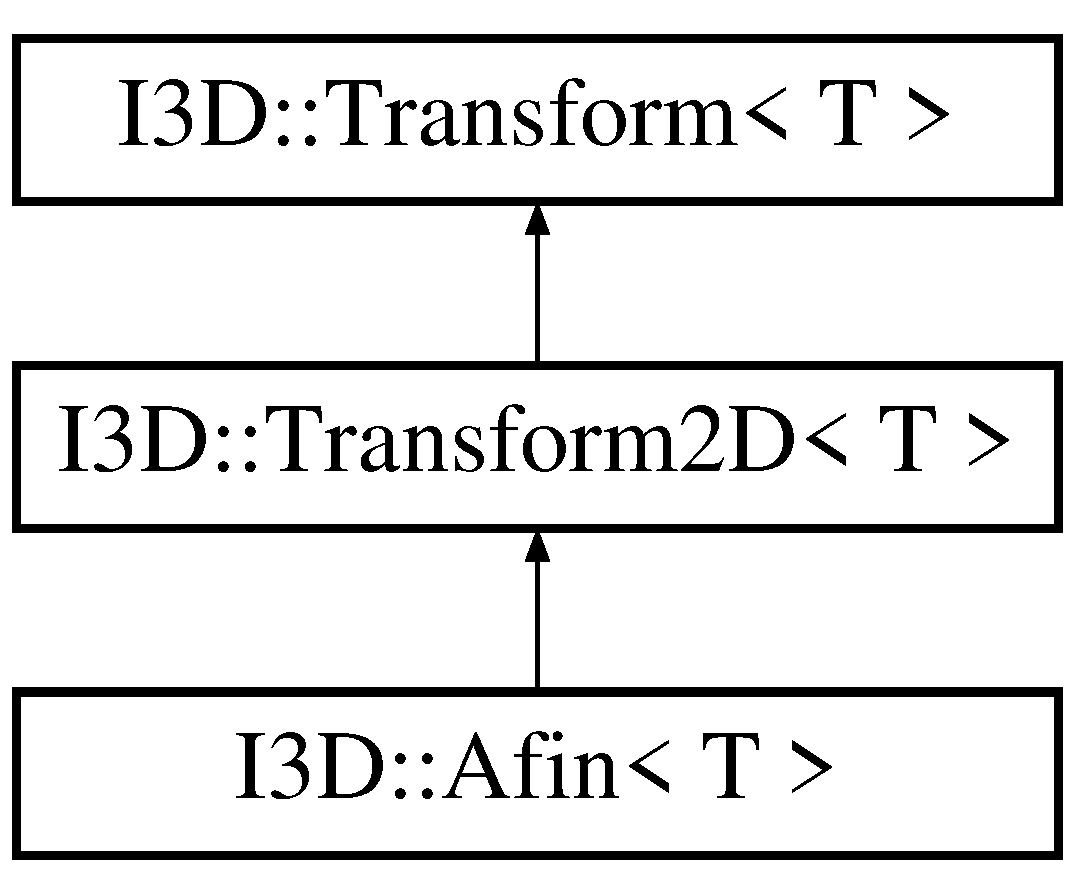
\includegraphics[height=3.000000cm]{class_i3_d_1_1_afin}
\end{center}
\end{figure}
\subsection*{Métodos públicos}
\begin{DoxyCompactItemize}
\item 
\hyperlink{class_i3_d_1_1_afin_ac54cf2d2c5335e8b05449ff56d2fd5fd}{Afin} ()
\begin{DoxyCompactList}\small\item\em Constructor por defecto. \end{DoxyCompactList}\item 
\hyperlink{class_i3_d_1_1_afin_a380364fda95636a4500637efd7cee797}{Afin} (T \hyperlink{class_i3_d_1_1_afin_aff62b2c4443c19c78940f4113e67183b}{x0}, T \hyperlink{class_i3_d_1_1_afin_ac687b5efb2b75262c7aeeb31a2792c34}{y0}, double scaleX, double scaleY, double rotation)
\begin{DoxyCompactList}\small\item\em Constructor. \end{DoxyCompactList}\item 
bool \hyperlink{group__trf2_d_group_gabe12d714c522dd1bf40f05f28c5aafe0}{compute} (const std\+::vector$<$ T $>$ \&pts1, const std\+::vector$<$ T $>$ \&pts2) override
\begin{DoxyCompactList}\small\item\em Calcula la transformación Helmert 2D entre dos sistemas diferentes a partir de dos conjuntos de puntos en cada sistema. \end{DoxyCompactList}\item 
void \hyperlink{group__trf2_d_group_gae1b65d232072a70d58ec72492a430521}{transform} (const std\+::vector$<$ T $>$ \&in, std\+::vector$<$ T $>$ $\ast$out, bool b\+Direct=true) const  override
\begin{DoxyCompactList}\small\item\em Transforma un conjunto de puntos en otro aplicando un helmert 2D. \end{DoxyCompactList}\item 
void \hyperlink{group__trf2_d_group_gaf2fb5278c5648034ef5f20c526866b77}{transform} (const T \&in, T $\ast$out, bool b\+Direct=true) const 
\begin{DoxyCompactList}\small\item\em Aplica un helmert 2D a un punto. \end{DoxyCompactList}\item 
T \hyperlink{group__trf2_d_group_ga8c7cfcf7b749b3adc69ebb6cfc0bb412}{transform} (const T \&in, bool b\+Direct=true) const 
\begin{DoxyCompactList}\small\item\em Aplica un helmert 2D a un punto. \end{DoxyCompactList}\item 
double \hyperlink{class_i3_d_1_1_afin_a72b19e66437e67f73b1f0a95eaa91c3f}{get\+Rotation} () const 
\begin{DoxyCompactList}\small\item\em Devuelve el giro. \end{DoxyCompactList}\item 
double \hyperlink{class_i3_d_1_1_afin_a1a4c447002e10793a6c187e028a50a13}{get\+ScaleX} () const 
\begin{DoxyCompactList}\small\item\em Devuelve la escala correspondiente al eje X. \end{DoxyCompactList}\item 
double \hyperlink{class_i3_d_1_1_afin_ad26bedc7f15fdd7e497b58cdb069cb7c}{get\+ScaleY} () const 
\begin{DoxyCompactList}\small\item\em Devuelve la escala correspondiente al eje Y. \end{DoxyCompactList}\item 
void \hyperlink{group__trf2_d_group_gaa6f479027bc96a8d58eaf52925822ecc}{set\+Parameters} (T \hyperlink{class_i3_d_1_1_afin_aff62b2c4443c19c78940f4113e67183b}{x0}, T \hyperlink{class_i3_d_1_1_afin_ac687b5efb2b75262c7aeeb31a2792c34}{y0}, double scaleX, double scaleY, double rotation)
\begin{DoxyCompactList}\small\item\em Establece los parámetros. \end{DoxyCompactList}\item 
void \hyperlink{group__trf2_d_group_ga07de5ad4be2f59ff5baa9b293211554d}{set\+Rotation} (double rotation)
\begin{DoxyCompactList}\small\item\em Establece la rotación de la transformación. \end{DoxyCompactList}\item 
void \hyperlink{group__trf2_d_group_ga33b6c90a0d7d957adb192d7768b574a1}{set\+ScaleX} (double scaleX)
\begin{DoxyCompactList}\small\item\em Establece la escala de la transformación en el eje X. \end{DoxyCompactList}\item 
void \hyperlink{group__trf2_d_group_ga2795a27b71c8e6364e71b828e042b6d7}{set\+ScaleY} (double scaleY)
\begin{DoxyCompactList}\small\item\em Establece la escala de la transformación en el eje Y. \end{DoxyCompactList}\end{DoxyCompactItemize}
\subsection*{Atributos públicos}
\begin{DoxyCompactItemize}
\item 
\hyperlink{class_i3_d_1_1_transform_ac087b4b8b9acb1b11a6caa2231d598c7}{sub\+\_\+type} \hyperlink{class_i3_d_1_1_afin_aff62b2c4443c19c78940f4113e67183b}{x0}
\begin{DoxyCompactList}\small\item\em Traslación en x. \end{DoxyCompactList}\item 
\hyperlink{class_i3_d_1_1_transform_ac087b4b8b9acb1b11a6caa2231d598c7}{sub\+\_\+type} \hyperlink{class_i3_d_1_1_afin_ac687b5efb2b75262c7aeeb31a2792c34}{y0}
\begin{DoxyCompactList}\small\item\em Traslación en y. \end{DoxyCompactList}\end{DoxyCompactItemize}
\subsection*{Otros miembros heredados}


\subsection{Descripción detallada}
\subsubsection*{template$<$typename T$>$\\*
class I3\+D\+::\+Afin$<$ T $>$}

Transformación \hyperlink{class_i3_d_1_1_afin}{Afin}. 

La Transformación Afín expresa la relación que existe (o la transformación que es preciso realizar) entre dos sistemas cartesianos que discrepan en la situación del origen, en la orientación de los ejes y en la unidad de medida a lo largo de los mismos de manera que dicha variación en unidad de medida es constante a lo largo de cada eje pero no entre los dos ejes.

\begin{quote}
a = scaleX $\ast$ cos(rotation); ~\newline
 b = scaleX $\ast$ sin(rotation); ~\newline
 c = -\/scaleY $\ast$ sin(rotation); ~\newline
 d = scaleY $\ast$ cos(rotation);

x\textquotesingle{} = a $\ast$ x + b $\ast$ y + X0 ~\newline
 y\textquotesingle{} = d $\ast$ y + c $\ast$ x + Y0 \end{quote}


\subsection{Documentación del constructor y destructor}
\index{I3\+D\+::\+Afin@{I3\+D\+::\+Afin}!Afin@{Afin}}
\index{Afin@{Afin}!I3\+D\+::\+Afin@{I3\+D\+::\+Afin}}
\subsubsection[{\texorpdfstring{Afin()}{Afin()}}]{\setlength{\rightskip}{0pt plus 5cm}template$<$typename T $>$ {\bf I3\+D\+::\+Afin}$<$ T $>$\+::{\bf Afin} (
\begin{DoxyParamCaption}
{}
\end{DoxyParamCaption}
)\hspace{0.3cm}{\ttfamily [inline]}}\hypertarget{class_i3_d_1_1_afin_ac54cf2d2c5335e8b05449ff56d2fd5fd}{}\label{class_i3_d_1_1_afin_ac54cf2d2c5335e8b05449ff56d2fd5fd}


Constructor por defecto. 

\index{I3\+D\+::\+Afin@{I3\+D\+::\+Afin}!Afin@{Afin}}
\index{Afin@{Afin}!I3\+D\+::\+Afin@{I3\+D\+::\+Afin}}
\subsubsection[{\texorpdfstring{Afin(\+T x0, T y0, double scale\+X, double scale\+Y, double rotation)}{Afin(T x0, T y0, double scaleX, double scaleY, double rotation)}}]{\setlength{\rightskip}{0pt plus 5cm}template$<$typename T $>$ {\bf I3\+D\+::\+Afin}$<$ T $>$\+::{\bf Afin} (
\begin{DoxyParamCaption}
\item[{T}]{x0, }
\item[{T}]{y0, }
\item[{double}]{scaleX, }
\item[{double}]{scaleY, }
\item[{double}]{rotation}
\end{DoxyParamCaption}
)\hspace{0.3cm}{\ttfamily [inline]}}\hypertarget{class_i3_d_1_1_afin_a380364fda95636a4500637efd7cee797}{}\label{class_i3_d_1_1_afin_a380364fda95636a4500637efd7cee797}


Constructor. 


\begin{DoxyParams}[1]{Parámetros}
\mbox{\tt in}  & {\em x0} & Traslación en el eje X \\
\hline
\mbox{\tt in}  & {\em y0} & Traslación en el eje Y \\
\hline
\mbox{\tt in}  & {\em scaleX} & Escala en el eje X \\
\hline
\mbox{\tt in}  & {\em scaleY} & Escala en el eje Y \\
\hline
\mbox{\tt in}  & {\em rotation} & Rotación \\
\hline
\end{DoxyParams}


\subsection{Documentación de las funciones miembro}
\index{I3\+D\+::\+Afin@{I3\+D\+::\+Afin}!get\+Rotation@{get\+Rotation}}
\index{get\+Rotation@{get\+Rotation}!I3\+D\+::\+Afin@{I3\+D\+::\+Afin}}
\subsubsection[{\texorpdfstring{get\+Rotation() const }{getRotation() const }}]{\setlength{\rightskip}{0pt plus 5cm}template$<$typename T $>$ double {\bf I3\+D\+::\+Afin}$<$ T $>$\+::get\+Rotation (
\begin{DoxyParamCaption}
{}
\end{DoxyParamCaption}
) const\hspace{0.3cm}{\ttfamily [inline]}}\hypertarget{class_i3_d_1_1_afin_a72b19e66437e67f73b1f0a95eaa91c3f}{}\label{class_i3_d_1_1_afin_a72b19e66437e67f73b1f0a95eaa91c3f}


Devuelve el giro. 

\begin{DoxyReturn}{Devuelve}
Ángulo de rotación en radianes 
\end{DoxyReturn}
\index{I3\+D\+::\+Afin@{I3\+D\+::\+Afin}!get\+ScaleX@{get\+ScaleX}}
\index{get\+ScaleX@{get\+ScaleX}!I3\+D\+::\+Afin@{I3\+D\+::\+Afin}}
\subsubsection[{\texorpdfstring{get\+Scale\+X() const }{getScaleX() const }}]{\setlength{\rightskip}{0pt plus 5cm}template$<$typename T $>$ double {\bf I3\+D\+::\+Afin}$<$ T $>$\+::get\+ScaleX (
\begin{DoxyParamCaption}
{}
\end{DoxyParamCaption}
) const\hspace{0.3cm}{\ttfamily [inline]}}\hypertarget{class_i3_d_1_1_afin_a1a4c447002e10793a6c187e028a50a13}{}\label{class_i3_d_1_1_afin_a1a4c447002e10793a6c187e028a50a13}


Devuelve la escala correspondiente al eje X. 

\begin{DoxyReturn}{Devuelve}
Escala eje X 
\end{DoxyReturn}
\index{I3\+D\+::\+Afin@{I3\+D\+::\+Afin}!get\+ScaleY@{get\+ScaleY}}
\index{get\+ScaleY@{get\+ScaleY}!I3\+D\+::\+Afin@{I3\+D\+::\+Afin}}
\subsubsection[{\texorpdfstring{get\+Scale\+Y() const }{getScaleY() const }}]{\setlength{\rightskip}{0pt plus 5cm}template$<$typename T $>$ double {\bf I3\+D\+::\+Afin}$<$ T $>$\+::get\+ScaleY (
\begin{DoxyParamCaption}
{}
\end{DoxyParamCaption}
) const\hspace{0.3cm}{\ttfamily [inline]}}\hypertarget{class_i3_d_1_1_afin_ad26bedc7f15fdd7e497b58cdb069cb7c}{}\label{class_i3_d_1_1_afin_ad26bedc7f15fdd7e497b58cdb069cb7c}


Devuelve la escala correspondiente al eje Y. 

\begin{DoxyReturn}{Devuelve}
Escala eje Y 
\end{DoxyReturn}


\subsection{Documentación de los datos miembro}
\index{I3\+D\+::\+Afin@{I3\+D\+::\+Afin}!x0@{x0}}
\index{x0@{x0}!I3\+D\+::\+Afin@{I3\+D\+::\+Afin}}
\subsubsection[{\texorpdfstring{x0}{x0}}]{\setlength{\rightskip}{0pt plus 5cm}template$<$typename T $>$ {\bf sub\+\_\+type} {\bf I3\+D\+::\+Afin}$<$ T $>$\+::x0}\hypertarget{class_i3_d_1_1_afin_aff62b2c4443c19c78940f4113e67183b}{}\label{class_i3_d_1_1_afin_aff62b2c4443c19c78940f4113e67183b}


Traslación en x. 

\index{I3\+D\+::\+Afin@{I3\+D\+::\+Afin}!y0@{y0}}
\index{y0@{y0}!I3\+D\+::\+Afin@{I3\+D\+::\+Afin}}
\subsubsection[{\texorpdfstring{y0}{y0}}]{\setlength{\rightskip}{0pt plus 5cm}template$<$typename T $>$ {\bf sub\+\_\+type} {\bf I3\+D\+::\+Afin}$<$ T $>$\+::y0}\hypertarget{class_i3_d_1_1_afin_ac687b5efb2b75262c7aeeb31a2792c34}{}\label{class_i3_d_1_1_afin_ac687b5efb2b75262c7aeeb31a2792c34}


Traslación en y. 



La documentación para esta clase fue generada a partir del siguiente fichero\+:\begin{DoxyCompactItemize}
\item 
D\+:/\+Desarrollo/tidop/src/\hyperlink{transform_8h}{transform.\+h}\end{DoxyCompactItemize}

\hypertarget{class_i3_d_1_1_bilateral_filter}{}\section{Referencia de la Clase I3D\+:\+:Bilateral\+Filter}
\label{class_i3_d_1_1_bilateral_filter}\index{I3\+D\+::\+Bilateral\+Filter@{I3\+D\+::\+Bilateral\+Filter}}


Filtro bilateral El filtro bilateral es un filtro no lineal que es muy eficaz en la eliminación de ruido manteniendo los bordes afilados. El valor de intensidad en cada pixel de la imagen es reemplazado por una media ponderada de los valores de intensidad de los píxeles cercanos.  




{\ttfamily \#include $<$Img\+Processing.\+h$>$}

Diagrama de herencias de I3D\+:\+:Bilateral\+Filter\begin{figure}[H]
\begin{center}
\leavevmode
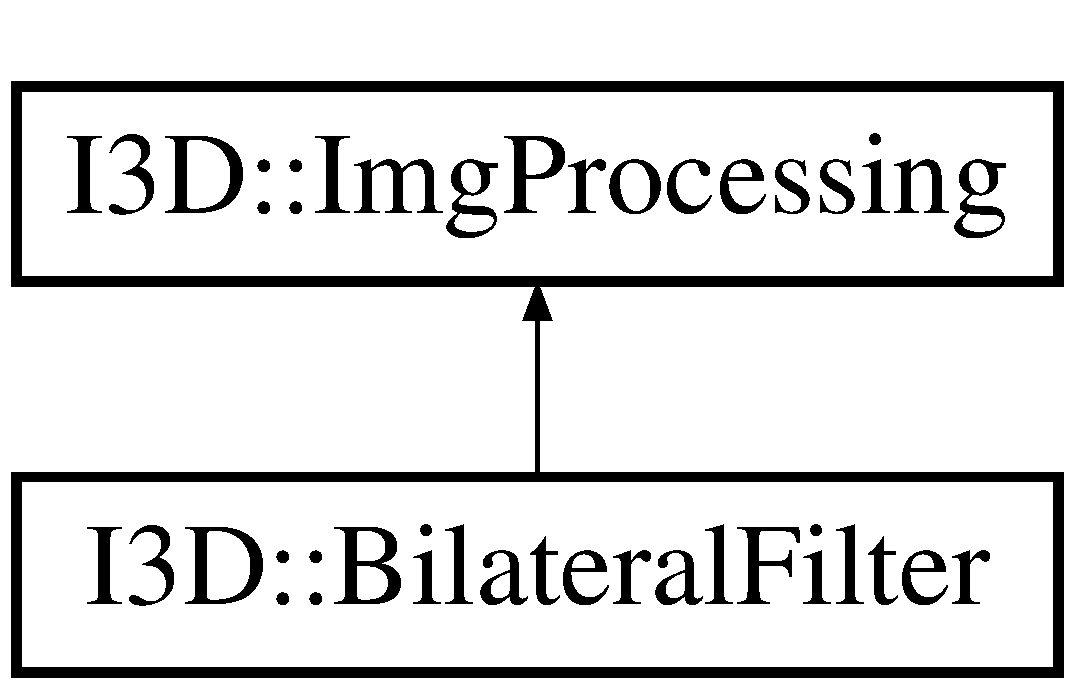
\includegraphics[height=2.000000cm]{class_i3_d_1_1_bilateral_filter}
\end{center}
\end{figure}
\subsection*{Métodos públicos}
\begin{DoxyCompactItemize}
\item 
\hyperlink{class_i3_d_1_1_bilateral_filter_af234e215c72e3a9a99e6e51679be0db8}{Bilateral\+Filter} (int diameter, double sigma\+Color, double sigma\+Space, int border\+Type=cv\+::\+B\+O\+R\+D\+E\+R\+\_\+\+D\+E\+F\+A\+U\+LT)
\begin{DoxyCompactList}\small\item\em Constructora de la clase \hyperlink{class_i3_d_1_1_bilateral_filter}{Bilateral\+Filter}. \end{DoxyCompactList}\item 
int \hyperlink{class_i3_d_1_1_bilateral_filter_a4b606ce8517fbd44dd1734e1a54bab10}{execute} (const cv\+::\+Mat \&mat\+In, cv\+::\+Mat $\ast$mat\+Out) const  override
\begin{DoxyCompactList}\small\item\em Aplica el filtro bilateral a una imagen. \end{DoxyCompactList}\item 
void \hyperlink{class_i3_d_1_1_bilateral_filter_acd2e8cf80d29f59a88e229dc7f966ed9}{set\+Parameters} (int diameter, double sigma\+Color, double sigma\+Space, int border\+Type=cv\+::\+B\+O\+R\+D\+E\+R\+\_\+\+D\+E\+F\+A\+U\+LT)
\begin{DoxyCompactList}\small\item\em Establece los parámetros del filtro bilateral. \end{DoxyCompactList}\end{DoxyCompactItemize}
\subsection*{Otros miembros heredados}


\subsection{Descripción detallada}
Filtro bilateral El filtro bilateral es un filtro no lineal que es muy eficaz en la eliminación de ruido manteniendo los bordes afilados. El valor de intensidad en cada pixel de la imagen es reemplazado por una media ponderada de los valores de intensidad de los píxeles cercanos. 

\subsection{Documentación del constructor y destructor}
\index{I3\+D\+::\+Bilateral\+Filter@{I3\+D\+::\+Bilateral\+Filter}!Bilateral\+Filter@{Bilateral\+Filter}}
\index{Bilateral\+Filter@{Bilateral\+Filter}!I3\+D\+::\+Bilateral\+Filter@{I3\+D\+::\+Bilateral\+Filter}}
\subsubsection[{\texorpdfstring{Bilateral\+Filter(int diameter, double sigma\+Color, double sigma\+Space, int border\+Type=cv\+::\+B\+O\+R\+D\+E\+R\+\_\+\+D\+E\+F\+A\+U\+L\+T)}{BilateralFilter(int diameter, double sigmaColor, double sigmaSpace, int borderType=cv::BORDER_DEFAULT)}}]{\setlength{\rightskip}{0pt plus 5cm}I3\+D\+::\+Bilateral\+Filter\+::\+Bilateral\+Filter (
\begin{DoxyParamCaption}
\item[{int}]{diameter, }
\item[{double}]{sigma\+Color, }
\item[{double}]{sigma\+Space, }
\item[{int}]{border\+Type = {\ttfamily cv\+:\+:BORDER\+\_\+DEFAULT}}
\end{DoxyParamCaption}
)\hspace{0.3cm}{\ttfamily [inline]}}\hypertarget{class_i3_d_1_1_bilateral_filter_af234e215c72e3a9a99e6e51679be0db8}{}\label{class_i3_d_1_1_bilateral_filter_af234e215c72e3a9a99e6e51679be0db8}


Constructora de la clase \hyperlink{class_i3_d_1_1_bilateral_filter}{Bilateral\+Filter}. 


\begin{DoxyParams}[1]{Parámetros}
\mbox{\tt in}  & {\em diameter} & \\
\hline
\mbox{\tt in}  & {\em sigma\+Color} & Núcleo gama para suavizar las diferencias en las intensidades \\
\hline
\mbox{\tt in}  & {\em sigma\+Space} & Núcleo espacial para suavizar las diferencias de coordenadas \\
\hline
\mbox{\tt in}  & {\em border\+Type} & \\
\hline
\end{DoxyParams}


\subsection{Documentación de las funciones miembro}
\index{I3\+D\+::\+Bilateral\+Filter@{I3\+D\+::\+Bilateral\+Filter}!execute@{execute}}
\index{execute@{execute}!I3\+D\+::\+Bilateral\+Filter@{I3\+D\+::\+Bilateral\+Filter}}
\subsubsection[{\texorpdfstring{execute(const cv\+::\+Mat \&mat\+In, cv\+::\+Mat $\ast$mat\+Out) const  override}{execute(const cv::Mat &matIn, cv::Mat *matOut) const  override}}]{\setlength{\rightskip}{0pt plus 5cm}int I3\+D\+::\+Bilateral\+Filter\+::execute (
\begin{DoxyParamCaption}
\item[{const cv\+::\+Mat \&}]{mat\+In, }
\item[{cv\+::\+Mat $\ast$}]{mat\+Out}
\end{DoxyParamCaption}
) const\hspace{0.3cm}{\ttfamily [override]}, {\ttfamily [virtual]}}\hypertarget{class_i3_d_1_1_bilateral_filter_a4b606ce8517fbd44dd1734e1a54bab10}{}\label{class_i3_d_1_1_bilateral_filter_a4b606ce8517fbd44dd1734e1a54bab10}


Aplica el filtro bilateral a una imagen. 


\begin{DoxyParams}[1]{Parámetros}
\mbox{\tt in}  & {\em mat\+In} & Imagen de entrada. \\
\hline
\mbox{\tt out}  & {\em mat\+Out} & Imagen de salida. \\
\hline
\end{DoxyParams}
\begin{DoxyReturn}{Devuelve}
Error. Si el proceso se ejecuta correctamente devuelve 0. 
\end{DoxyReturn}


Implementa \hyperlink{class_i3_d_1_1_img_processing_a74195f05bbf034566e9ff6e10f3af4c9}{I3\+D\+::\+Img\+Processing}.

\index{I3\+D\+::\+Bilateral\+Filter@{I3\+D\+::\+Bilateral\+Filter}!set\+Parameters@{set\+Parameters}}
\index{set\+Parameters@{set\+Parameters}!I3\+D\+::\+Bilateral\+Filter@{I3\+D\+::\+Bilateral\+Filter}}
\subsubsection[{\texorpdfstring{set\+Parameters(int diameter, double sigma\+Color, double sigma\+Space, int border\+Type=cv\+::\+B\+O\+R\+D\+E\+R\+\_\+\+D\+E\+F\+A\+U\+L\+T)}{setParameters(int diameter, double sigmaColor, double sigmaSpace, int borderType=cv::BORDER_DEFAULT)}}]{\setlength{\rightskip}{0pt plus 5cm}void I3\+D\+::\+Bilateral\+Filter\+::set\+Parameters (
\begin{DoxyParamCaption}
\item[{int}]{diameter, }
\item[{double}]{sigma\+Color, }
\item[{double}]{sigma\+Space, }
\item[{int}]{border\+Type = {\ttfamily cv\+:\+:BORDER\+\_\+DEFAULT}}
\end{DoxyParamCaption}
)}\hypertarget{class_i3_d_1_1_bilateral_filter_acd2e8cf80d29f59a88e229dc7f966ed9}{}\label{class_i3_d_1_1_bilateral_filter_acd2e8cf80d29f59a88e229dc7f966ed9}


Establece los parámetros del filtro bilateral. 


\begin{DoxyParams}[1]{Parámetros}
\mbox{\tt in}  & {\em diameter} & \\
\hline
\mbox{\tt in}  & {\em sigma\+Color} & Núcleo gama para suavizar las diferencias en las intensidades \\
\hline
\mbox{\tt in}  & {\em sigma\+Space} & Núcleo espacial para suavizar las diferencias de coordenadas \\
\hline
\mbox{\tt in}  & {\em border\+Type} & \\
\hline
\end{DoxyParams}


La documentación para esta clase fue generada a partir de los siguientes ficheros\+:\begin{DoxyCompactItemize}
\item 
C\+:/\+Desarrollo/tidop/src/\hyperlink{_img_processing_8h}{Img\+Processing.\+h}\item 
C\+:/\+Desarrollo/tidop/src/\hyperlink{_img_processing_8cpp}{Img\+Processing.\+cpp}\end{DoxyCompactItemize}

\hypertarget{class_i3_d_1_1_binarize}{}\section{Referencia de la Clase I3D\+:\+:Binarize}
\label{class_i3_d_1_1_binarize}\index{I3\+D\+::\+Binarize@{I3\+D\+::\+Binarize}}


Clase \hyperlink{class_i3_d_1_1_binarize}{Binarize} Convierte una imagen a binaria.  




{\ttfamily \#include $<$Img\+Processing.\+h$>$}

Diagrama de herencias de I3D\+:\+:Binarize\begin{figure}[H]
\begin{center}
\leavevmode
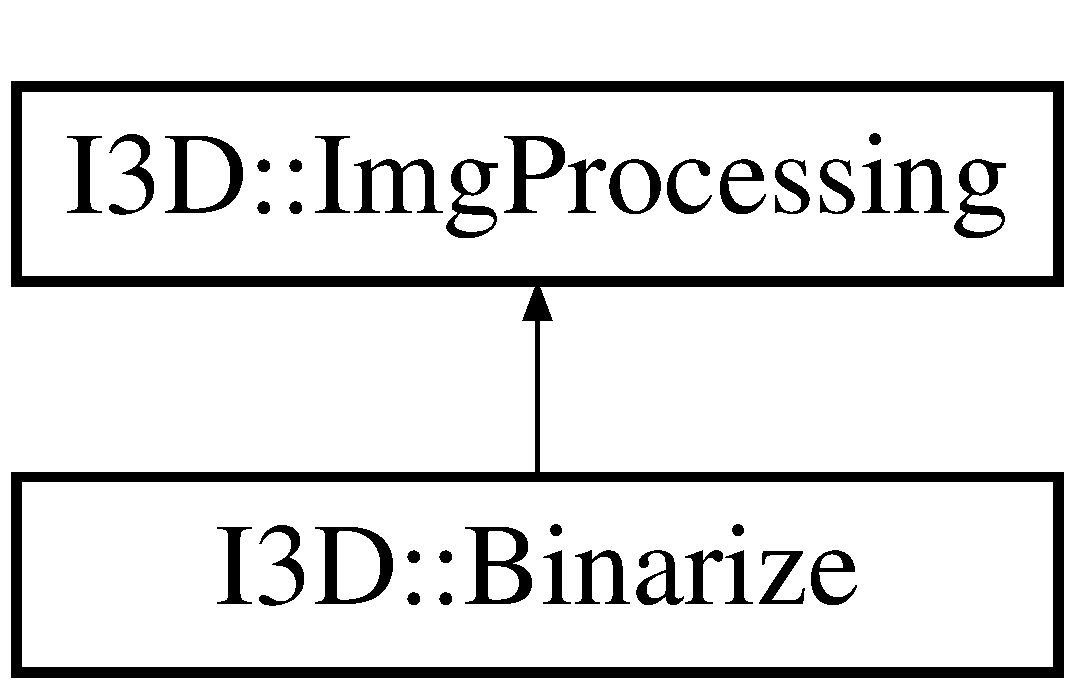
\includegraphics[height=2.000000cm]{class_i3_d_1_1_binarize}
\end{center}
\end{figure}
\subsection*{Métodos públicos}
\begin{DoxyCompactItemize}
\item 
\hyperlink{class_i3_d_1_1_binarize_a1c91d13b3c1ce63366da49291cbac5c7}{Binarize} (double thresh=0., double max\+Val=0., bool b\+Inverse=false)
\begin{DoxyCompactList}\small\item\em Constructora de la clase \hyperlink{class_i3_d_1_1_binarize}{Binarize} Si thresh y max\+Val son 0 se calculan internamente a partir de la media y desviación típica. \end{DoxyCompactList}\item 
int \hyperlink{class_i3_d_1_1_binarize_a2630da33f5cc1c9fe80c991ffd84f613}{execute} (const cv\+::\+Mat \&mat\+In, cv\+::\+Mat $\ast$mat\+Out) const  override
\begin{DoxyCompactList}\small\item\em Ejecuta el proceso. \end{DoxyCompactList}\item 
void \hyperlink{class_i3_d_1_1_binarize_aa598d2d5cdc271fdb2f395c0c76fd012}{set\+Parameters} (double thresh, double max\+Val, bool b\+Inverse=false)
\begin{DoxyCompactList}\small\item\em Establece los parámetros. \end{DoxyCompactList}\item 
void \hyperlink{class_i3_d_1_1_binarize_a0c8b496fa8e2f0558f5ab15937c0e69c}{set\+Inverse} (bool inverse=true)
\begin{DoxyCompactList}\small\item\em Binarización inversa. \end{DoxyCompactList}\item 
bool \hyperlink{class_i3_d_1_1_binarize_a7061a766fd5495aee6301965791f92c3}{get\+Inverse} () const 
\begin{DoxyCompactList}\small\item\em Get\+Inverse. \end{DoxyCompactList}\end{DoxyCompactItemize}
\subsection*{Otros miembros heredados}


\subsection{Descripción detallada}
Clase \hyperlink{class_i3_d_1_1_binarize}{Binarize} Convierte una imagen a binaria. 

\subsection{Documentación del constructor y destructor}
\index{I3\+D\+::\+Binarize@{I3\+D\+::\+Binarize}!Binarize@{Binarize}}
\index{Binarize@{Binarize}!I3\+D\+::\+Binarize@{I3\+D\+::\+Binarize}}
\subsubsection[{\texorpdfstring{Binarize(double thresh=0., double max\+Val=0., bool b\+Inverse=false)}{Binarize(double thresh=0., double maxVal=0., bool bInverse=false)}}]{\setlength{\rightskip}{0pt plus 5cm}I3\+D\+::\+Binarize\+::\+Binarize (
\begin{DoxyParamCaption}
\item[{double}]{thresh = {\ttfamily 0.}, }
\item[{double}]{max\+Val = {\ttfamily 0.}, }
\item[{bool}]{b\+Inverse = {\ttfamily false}}
\end{DoxyParamCaption}
)\hspace{0.3cm}{\ttfamily [inline]}}\hypertarget{class_i3_d_1_1_binarize_a1c91d13b3c1ce63366da49291cbac5c7}{}\label{class_i3_d_1_1_binarize_a1c91d13b3c1ce63366da49291cbac5c7}


Constructora de la clase \hyperlink{class_i3_d_1_1_binarize}{Binarize} Si thresh y max\+Val son 0 se calculan internamente a partir de la media y desviación típica. 


\begin{DoxyParams}{Parámetros}
{\em thresh} & Umbral \\
\hline
{\em max\+Val} & Valor máximo \\
\hline
{\em b\+Inverse} & Binarización inversa \\
\hline
\end{DoxyParams}


\subsection{Documentación de las funciones miembro}
\index{I3\+D\+::\+Binarize@{I3\+D\+::\+Binarize}!execute@{execute}}
\index{execute@{execute}!I3\+D\+::\+Binarize@{I3\+D\+::\+Binarize}}
\subsubsection[{\texorpdfstring{execute(const cv\+::\+Mat \&mat\+In, cv\+::\+Mat $\ast$mat\+Out) const  override}{execute(const cv::Mat &matIn, cv::Mat *matOut) const  override}}]{\setlength{\rightskip}{0pt plus 5cm}int I3\+D\+::\+Binarize\+::execute (
\begin{DoxyParamCaption}
\item[{const cv\+::\+Mat \&}]{mat\+In, }
\item[{cv\+::\+Mat $\ast$}]{mat\+Out}
\end{DoxyParamCaption}
) const\hspace{0.3cm}{\ttfamily [override]}, {\ttfamily [virtual]}}\hypertarget{class_i3_d_1_1_binarize_a2630da33f5cc1c9fe80c991ffd84f613}{}\label{class_i3_d_1_1_binarize_a2630da33f5cc1c9fe80c991ffd84f613}


Ejecuta el proceso. 


\begin{DoxyParams}[1]{Parámetros}
\mbox{\tt in}  & {\em mat\+In} & Imagen de entrada \\
\hline
\mbox{\tt out}  & {\em mat\+Out} & Imagen de salida \\
\hline
\end{DoxyParams}
\begin{DoxyReturn}{Devuelve}
Error. Si los procesos se ejecutan correctamente devuelve 0. 
\end{DoxyReturn}


Implementa \hyperlink{class_i3_d_1_1_img_processing_a74195f05bbf034566e9ff6e10f3af4c9}{I3\+D\+::\+Img\+Processing}.

\index{I3\+D\+::\+Binarize@{I3\+D\+::\+Binarize}!get\+Inverse@{get\+Inverse}}
\index{get\+Inverse@{get\+Inverse}!I3\+D\+::\+Binarize@{I3\+D\+::\+Binarize}}
\subsubsection[{\texorpdfstring{get\+Inverse() const }{getInverse() const }}]{\setlength{\rightskip}{0pt plus 5cm}bool I3\+D\+::\+Binarize\+::get\+Inverse (
\begin{DoxyParamCaption}
{}
\end{DoxyParamCaption}
) const\hspace{0.3cm}{\ttfamily [inline]}}\hypertarget{class_i3_d_1_1_binarize_a7061a766fd5495aee6301965791f92c3}{}\label{class_i3_d_1_1_binarize_a7061a766fd5495aee6301965791f92c3}


Get\+Inverse. 

\begin{DoxyReturn}{Devuelve}

\end{DoxyReturn}
\index{I3\+D\+::\+Binarize@{I3\+D\+::\+Binarize}!set\+Inverse@{set\+Inverse}}
\index{set\+Inverse@{set\+Inverse}!I3\+D\+::\+Binarize@{I3\+D\+::\+Binarize}}
\subsubsection[{\texorpdfstring{set\+Inverse(bool inverse=true)}{setInverse(bool inverse=true)}}]{\setlength{\rightskip}{0pt plus 5cm}void I3\+D\+::\+Binarize\+::set\+Inverse (
\begin{DoxyParamCaption}
\item[{bool}]{inverse = {\ttfamily true}}
\end{DoxyParamCaption}
)\hspace{0.3cm}{\ttfamily [inline]}}\hypertarget{class_i3_d_1_1_binarize_a0c8b496fa8e2f0558f5ab15937c0e69c}{}\label{class_i3_d_1_1_binarize_a0c8b496fa8e2f0558f5ab15937c0e69c}


Binarización inversa. 


\begin{DoxyParams}[1]{Parámetros}
\mbox{\tt in}  & {\em inverse} & \\
\hline
\end{DoxyParams}
\index{I3\+D\+::\+Binarize@{I3\+D\+::\+Binarize}!set\+Parameters@{set\+Parameters}}
\index{set\+Parameters@{set\+Parameters}!I3\+D\+::\+Binarize@{I3\+D\+::\+Binarize}}
\subsubsection[{\texorpdfstring{set\+Parameters(double thresh, double max\+Val, bool b\+Inverse=false)}{setParameters(double thresh, double maxVal, bool bInverse=false)}}]{\setlength{\rightskip}{0pt plus 5cm}void I3\+D\+::\+Binarize\+::set\+Parameters (
\begin{DoxyParamCaption}
\item[{double}]{thresh, }
\item[{double}]{max\+Val, }
\item[{bool}]{b\+Inverse = {\ttfamily false}}
\end{DoxyParamCaption}
)}\hypertarget{class_i3_d_1_1_binarize_aa598d2d5cdc271fdb2f395c0c76fd012}{}\label{class_i3_d_1_1_binarize_aa598d2d5cdc271fdb2f395c0c76fd012}


Establece los parámetros. 


\begin{DoxyParams}[1]{Parámetros}
\mbox{\tt in}  & {\em thresh} & Umbral \\
\hline
\mbox{\tt in}  & {\em max\+Val} & Valor máximo \\
\hline
\mbox{\tt in}  & {\em b\+Inverse} & Binarización inversa \\
\hline
\end{DoxyParams}


La documentación para esta clase fue generada a partir de los siguientes ficheros\+:\begin{DoxyCompactItemize}
\item 
D\+:/\+Desarrollo/tidop/src/\hyperlink{_img_processing_8h}{Img\+Processing.\+h}\item 
D\+:/\+Desarrollo/tidop/src/\hyperlink{_img_processing_8cpp}{Img\+Processing.\+cpp}\end{DoxyCompactItemize}

\hypertarget{class_i3_d_1_1_black_hat}{}\section{Referencia de la Clase I3D\+:\+:Black\+Hat}
\label{class_i3_d_1_1_black_hat}\index{I3\+D\+::\+Black\+Hat@{I3\+D\+::\+Black\+Hat}}


Operación morfológica Black Hat Esta operación consite en aplicar un cierre a una imagen y restar el resultado por la la imagen original.  




{\ttfamily \#include $<$Img\+Processing.\+h$>$}

Diagrama de herencias de I3D\+:\+:Black\+Hat\begin{figure}[H]
\begin{center}
\leavevmode
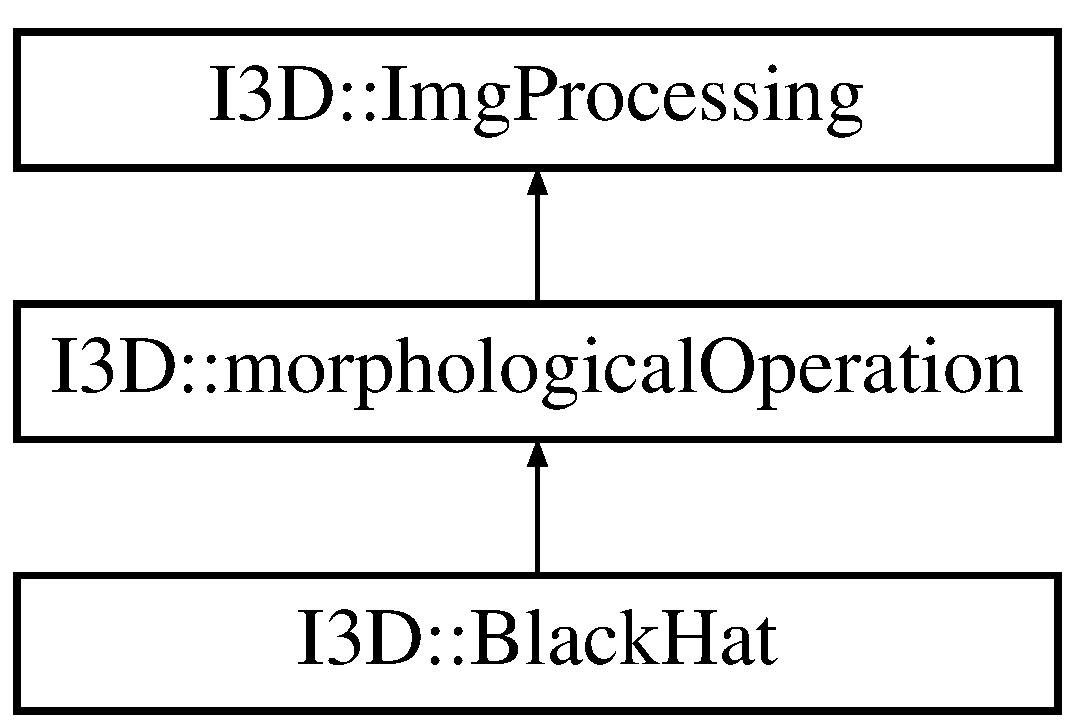
\includegraphics[height=3.000000cm]{class_i3_d_1_1_black_hat}
\end{center}
\end{figure}
\subsection*{Métodos públicos}
\begin{DoxyCompactItemize}
\item 
\hyperlink{class_i3_d_1_1_black_hat_ac3428524b0f9ed91a353874e5570e905}{Black\+Hat} (int size, cv\+::\+Morph\+Shapes shapes=cv\+::\+M\+O\+R\+P\+H\+\_\+\+R\+E\+CT, cv\+::\+Point anchor=cv\+::\+Point(-\/1,-\/1), int iterations=1, int border\+Type=cv\+::\+B\+O\+R\+D\+E\+R\+\_\+\+C\+O\+N\+S\+T\+A\+NT, const cv\+::\+Scalar \&border\+Value=cv\+::morphology\+Default\+Border\+Value())
\begin{DoxyCompactList}\small\item\em Constructora clase \hyperlink{class_i3_d_1_1_closing}{Closing}. \end{DoxyCompactList}\end{DoxyCompactItemize}
\subsection*{Otros miembros heredados}


\subsection{Descripción detallada}
Operación morfológica Black Hat Esta operación consite en aplicar un cierre a una imagen y restar el resultado por la la imagen original. 

\subsection{Documentación del constructor y destructor}
\index{I3\+D\+::\+Black\+Hat@{I3\+D\+::\+Black\+Hat}!Black\+Hat@{Black\+Hat}}
\index{Black\+Hat@{Black\+Hat}!I3\+D\+::\+Black\+Hat@{I3\+D\+::\+Black\+Hat}}
\subsubsection[{\texorpdfstring{Black\+Hat(int size, cv\+::\+Morph\+Shapes shapes=cv\+::\+M\+O\+R\+P\+H\+\_\+\+R\+E\+C\+T, cv\+::\+Point anchor=cv\+::\+Point(-\/1,-\/1), int iterations=1, int border\+Type=cv\+::\+B\+O\+R\+D\+E\+R\+\_\+\+C\+O\+N\+S\+T\+A\+N\+T, const cv\+::\+Scalar \&border\+Value=cv\+::morphology\+Default\+Border\+Value())}{BlackHat(int size, cv::MorphShapes shapes=cv::MORPH_RECT, cv::Point anchor=cv::Point(-1,-1), int iterations=1, int borderType=cv::BORDER_CONSTANT, const cv::Scalar &borderValue=cv::morphologyDefaultBorderValue())}}]{\setlength{\rightskip}{0pt plus 5cm}I3\+D\+::\+Black\+Hat\+::\+Black\+Hat (
\begin{DoxyParamCaption}
\item[{int}]{size, }
\item[{cv\+::\+Morph\+Shapes}]{shapes = {\ttfamily cv\+:\+:MORPH\+\_\+RECT}, }
\item[{cv\+::\+Point}]{anchor = {\ttfamily cv\+:\+:Point(-\/1,~-\/1)}, }
\item[{int}]{iterations = {\ttfamily 1}, }
\item[{int}]{border\+Type = {\ttfamily cv\+:\+:BORDER\+\_\+CONSTANT}, }
\item[{const cv\+::\+Scalar \&}]{border\+Value = {\ttfamily cv\+:\+:morphologyDefaultBorderValue()}}
\end{DoxyParamCaption}
)\hspace{0.3cm}{\ttfamily [inline]}}\hypertarget{class_i3_d_1_1_black_hat_ac3428524b0f9ed91a353874e5570e905}{}\label{class_i3_d_1_1_black_hat_ac3428524b0f9ed91a353874e5570e905}


Constructora clase \hyperlink{class_i3_d_1_1_closing}{Closing}. 


\begin{DoxyParams}[1]{Parámetros}
\mbox{\tt in}  & {\em size} & \\
\hline
\mbox{\tt in}  & {\em type} & \\
\hline
\mbox{\tt in}  & {\em anchor} & Punto de anclaje. Por defecto es el centro del kernel \\
\hline
\mbox{\tt in}  & {\em iterations} & \\
\hline
\mbox{\tt in}  & {\em border\+Type} & Método de extrapolación \\
\hline
\mbox{\tt in}  & {\em border\+Value} & \\
\hline
\end{DoxyParams}


La documentación para esta clase fue generada a partir del siguiente fichero\+:\begin{DoxyCompactItemize}
\item 
D\+:/\+Desarrollo/tidop/src/\hyperlink{_img_processing_8h}{Img\+Processing.\+h}\end{DoxyCompactItemize}

\hypertarget{class_i3_d_1_1_blur}{}\section{Referencia de la Clase I3D\+:\+:Blur}
\label{class_i3_d_1_1_blur}\index{I3\+D\+::\+Blur@{I3\+D\+::\+Blur}}


Filtro de desenfoque Provoca un suavizado en la imagen resultante.  




{\ttfamily \#include $<$Img\+Processing.\+h$>$}

Diagrama de herencias de I3D\+:\+:Blur\begin{figure}[H]
\begin{center}
\leavevmode
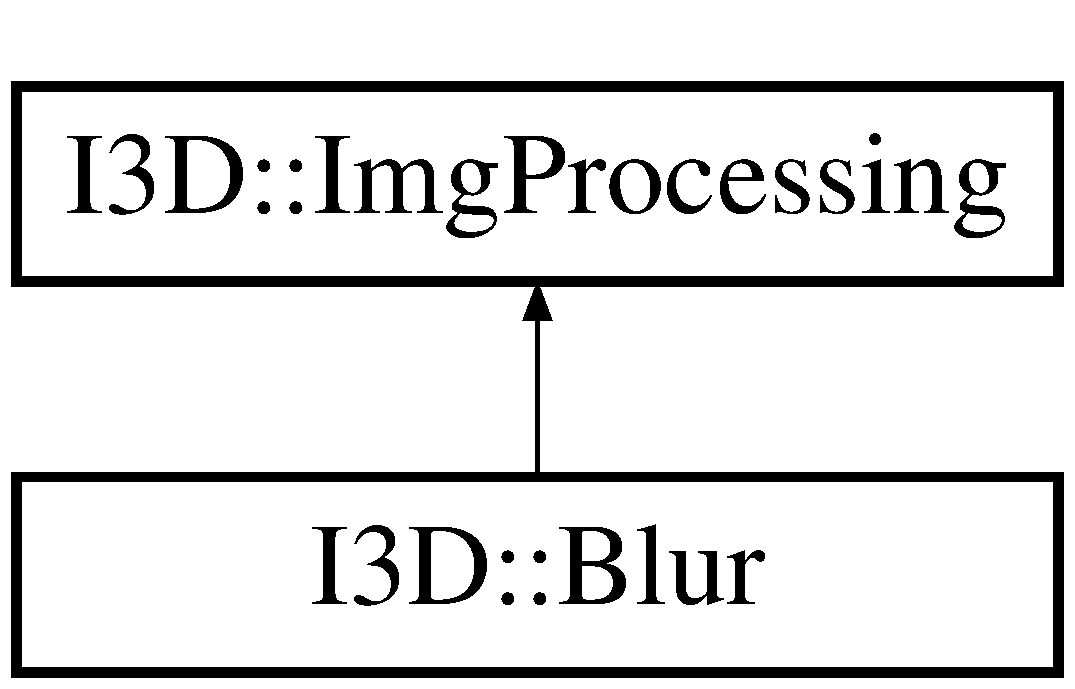
\includegraphics[height=2.000000cm]{class_i3_d_1_1_blur}
\end{center}
\end{figure}
\subsection*{Métodos públicos}
\begin{DoxyCompactItemize}
\item 
\hyperlink{class_i3_d_1_1_blur_a96bf63044e9fad0a439073ca8fb53e7a}{Blur} (cv\+::\+Size ksize, cv\+::\+Point anchor=cv\+::\+Point(-\/1,-\/1), int border\+Type=cv\+::\+B\+O\+R\+D\+E\+R\+\_\+\+D\+E\+F\+A\+U\+LT)
\begin{DoxyCompactList}\small\item\em Constructora de la clase. \end{DoxyCompactList}\item 
int \hyperlink{class_i3_d_1_1_blur_a9bc99ea12ce16294f415f67ce467a81b}{execute} (const cv\+::\+Mat \&mat\+In, cv\+::\+Mat $\ast$mat\+Out) const  override
\begin{DoxyCompactList}\small\item\em Aplica el filtro de desenfoque. \end{DoxyCompactList}\item 
void \hyperlink{class_i3_d_1_1_blur_a5a141450b0eae0a7a44eea935c0bc418}{set\+Parameters} (cv\+::\+Size ksize, cv\+::\+Point anchor=cv\+::\+Point(-\/1,-\/1), int border\+Type=cv\+::\+B\+O\+R\+D\+E\+R\+\_\+\+D\+E\+F\+A\+U\+LT)
\begin{DoxyCompactList}\small\item\em Establece los parámetros del filtro. \end{DoxyCompactList}\end{DoxyCompactItemize}
\subsection*{Otros miembros heredados}


\subsection{Descripción detallada}
Filtro de desenfoque Provoca un suavizado en la imagen resultante. 

\subsection{Documentación del constructor y destructor}
\index{I3\+D\+::\+Blur@{I3\+D\+::\+Blur}!Blur@{Blur}}
\index{Blur@{Blur}!I3\+D\+::\+Blur@{I3\+D\+::\+Blur}}
\subsubsection[{\texorpdfstring{Blur(cv\+::\+Size ksize, cv\+::\+Point anchor=cv\+::\+Point(-\/1,-\/1), int border\+Type=cv\+::\+B\+O\+R\+D\+E\+R\+\_\+\+D\+E\+F\+A\+U\+L\+T)}{Blur(cv::Size ksize, cv::Point anchor=cv::Point(-1,-1), int borderType=cv::BORDER_DEFAULT)}}]{\setlength{\rightskip}{0pt plus 5cm}I3\+D\+::\+Blur\+::\+Blur (
\begin{DoxyParamCaption}
\item[{cv\+::\+Size}]{ksize, }
\item[{cv\+::\+Point}]{anchor = {\ttfamily cv\+:\+:Point(-\/1,~-\/1)}, }
\item[{int}]{border\+Type = {\ttfamily cv\+:\+:BORDER\+\_\+DEFAULT}}
\end{DoxyParamCaption}
)\hspace{0.3cm}{\ttfamily [inline]}}\hypertarget{class_i3_d_1_1_blur_a96bf63044e9fad0a439073ca8fb53e7a}{}\label{class_i3_d_1_1_blur_a96bf63044e9fad0a439073ca8fb53e7a}


Constructora de la clase. 


\begin{DoxyParams}[1]{Parámetros}
\mbox{\tt in}  & {\em ksize} & Tamaño del kernel \\
\hline
\mbox{\tt in}  & {\em anchor} & Punto de anclaje \\
\hline
\mbox{\tt in}  & {\em border\+Type} & Tipo de borde \\
\hline
\end{DoxyParams}


\subsection{Documentación de las funciones miembro}
\index{I3\+D\+::\+Blur@{I3\+D\+::\+Blur}!execute@{execute}}
\index{execute@{execute}!I3\+D\+::\+Blur@{I3\+D\+::\+Blur}}
\subsubsection[{\texorpdfstring{execute(const cv\+::\+Mat \&mat\+In, cv\+::\+Mat $\ast$mat\+Out) const  override}{execute(const cv::Mat &matIn, cv::Mat *matOut) const  override}}]{\setlength{\rightskip}{0pt plus 5cm}int I3\+D\+::\+Blur\+::execute (
\begin{DoxyParamCaption}
\item[{const cv\+::\+Mat \&}]{mat\+In, }
\item[{cv\+::\+Mat $\ast$}]{mat\+Out}
\end{DoxyParamCaption}
) const\hspace{0.3cm}{\ttfamily [override]}, {\ttfamily [virtual]}}\hypertarget{class_i3_d_1_1_blur_a9bc99ea12ce16294f415f67ce467a81b}{}\label{class_i3_d_1_1_blur_a9bc99ea12ce16294f415f67ce467a81b}


Aplica el filtro de desenfoque. 


\begin{DoxyParams}[1]{Parámetros}
\mbox{\tt in}  & {\em mat\+In} & Imagen de entrada. \\
\hline
\mbox{\tt out}  & {\em mat\+Out} & Imagen de salida. \\
\hline
\end{DoxyParams}
\begin{DoxyReturn}{Devuelve}
Error. Si el proceso se ejecuta correctamente devuelve 0. 
\end{DoxyReturn}


Implementa \hyperlink{class_i3_d_1_1_img_processing_a74195f05bbf034566e9ff6e10f3af4c9}{I3\+D\+::\+Img\+Processing}.

\index{I3\+D\+::\+Blur@{I3\+D\+::\+Blur}!set\+Parameters@{set\+Parameters}}
\index{set\+Parameters@{set\+Parameters}!I3\+D\+::\+Blur@{I3\+D\+::\+Blur}}
\subsubsection[{\texorpdfstring{set\+Parameters(cv\+::\+Size ksize, cv\+::\+Point anchor=cv\+::\+Point(-\/1,-\/1), int border\+Type=cv\+::\+B\+O\+R\+D\+E\+R\+\_\+\+D\+E\+F\+A\+U\+L\+T)}{setParameters(cv::Size ksize, cv::Point anchor=cv::Point(-1,-1), int borderType=cv::BORDER_DEFAULT)}}]{\setlength{\rightskip}{0pt plus 5cm}void I3\+D\+::\+Blur\+::set\+Parameters (
\begin{DoxyParamCaption}
\item[{cv\+::\+Size}]{ksize, }
\item[{cv\+::\+Point}]{anchor = {\ttfamily cv\+:\+:Point(-\/1,~-\/1)}, }
\item[{int}]{border\+Type = {\ttfamily cv\+:\+:BORDER\+\_\+DEFAULT}}
\end{DoxyParamCaption}
)}\hypertarget{class_i3_d_1_1_blur_a5a141450b0eae0a7a44eea935c0bc418}{}\label{class_i3_d_1_1_blur_a5a141450b0eae0a7a44eea935c0bc418}


Establece los parámetros del filtro. 


\begin{DoxyParams}[1]{Parámetros}
\mbox{\tt in}  & {\em ksize} & Tamaño del kernel \\
\hline
\mbox{\tt in}  & {\em anchor} & Punto de anclaje \\
\hline
\mbox{\tt in}  & {\em border\+Type} & Tipo de borde \\
\hline
\end{DoxyParams}


La documentación para esta clase fue generada a partir de los siguientes ficheros\+:\begin{DoxyCompactItemize}
\item 
D\+:/\+Desarrollo/tidop/src/\hyperlink{_img_processing_8h}{Img\+Processing.\+h}\item 
D\+:/\+Desarrollo/tidop/src/\hyperlink{_img_processing_8cpp}{Img\+Processing.\+cpp}\end{DoxyCompactItemize}

\hypertarget{class_i3_d_1_1_box_filter}{}\section{Referencia de la Clase I3D\+:\+:Box\+Filter}
\label{class_i3_d_1_1_box_filter}\index{I3\+D\+::\+Box\+Filter@{I3\+D\+::\+Box\+Filter}}


Filtro de desenfoque Provoca un suavizado en la imagen resultante.  




{\ttfamily \#include $<$Img\+Processing.\+h$>$}

Diagrama de herencias de I3D\+:\+:Box\+Filter\begin{figure}[H]
\begin{center}
\leavevmode
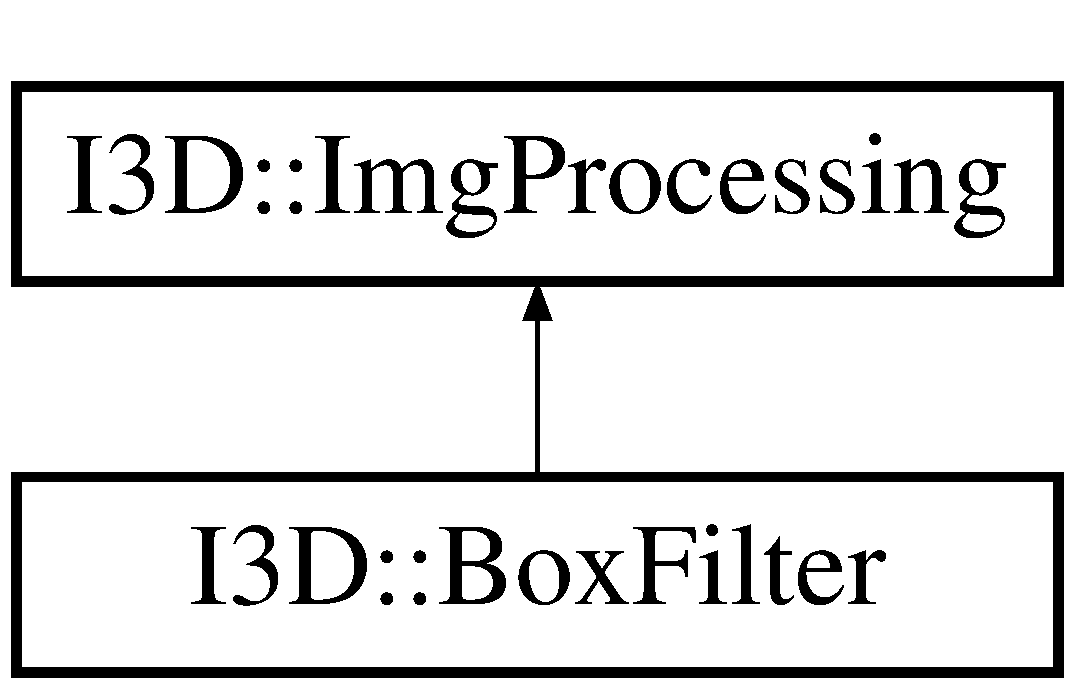
\includegraphics[height=2.000000cm]{class_i3_d_1_1_box_filter}
\end{center}
\end{figure}
\subsection*{Métodos públicos}
\begin{DoxyCompactItemize}
\item 
\hyperlink{class_i3_d_1_1_box_filter_a9b4a1eae6fd00f282c831becf3e5b923}{Box\+Filter} (int ddepth, cv\+::\+Size ksize, cv\+::\+Point anchor=cv\+::\+Point(-\/1,-\/1), bool normalize=true, int border\+Type=cv\+::\+B\+O\+R\+D\+E\+R\+\_\+\+D\+E\+F\+A\+U\+LT)
\begin{DoxyCompactList}\small\item\em Constructora de la clase. \end{DoxyCompactList}\item 
int \hyperlink{class_i3_d_1_1_box_filter_aaea2d395620162626a7b16b85ae44c42}{execute} (const cv\+::\+Mat \&mat\+In, cv\+::\+Mat $\ast$mat\+Out) const  override
\begin{DoxyCompactList}\small\item\em Aplica el filtro de desenfoque. \end{DoxyCompactList}\item 
void \hyperlink{class_i3_d_1_1_box_filter_a41f1b6c62f43fab9571432d0852a2a41}{set\+Parameters} (int ddepth, cv\+::\+Size ksize, cv\+::\+Point anchor=cv\+::\+Point(-\/1,-\/1), bool normalize=true, int border\+Type=cv\+::\+B\+O\+R\+D\+E\+R\+\_\+\+D\+E\+F\+A\+U\+LT)
\begin{DoxyCompactList}\small\item\em Establece los parámetros del filtro. \end{DoxyCompactList}\end{DoxyCompactItemize}
\subsection*{Otros miembros heredados}


\subsection{Descripción detallada}
Filtro de desenfoque Provoca un suavizado en la imagen resultante. 

\subsection{Documentación del constructor y destructor}
\index{I3\+D\+::\+Box\+Filter@{I3\+D\+::\+Box\+Filter}!Box\+Filter@{Box\+Filter}}
\index{Box\+Filter@{Box\+Filter}!I3\+D\+::\+Box\+Filter@{I3\+D\+::\+Box\+Filter}}
\subsubsection[{\texorpdfstring{Box\+Filter(int ddepth, cv\+::\+Size ksize, cv\+::\+Point anchor=cv\+::\+Point(-\/1,-\/1), bool normalize=true, int border\+Type=cv\+::\+B\+O\+R\+D\+E\+R\+\_\+\+D\+E\+F\+A\+U\+L\+T)}{BoxFilter(int ddepth, cv::Size ksize, cv::Point anchor=cv::Point(-1,-1), bool normalize=true, int borderType=cv::BORDER_DEFAULT)}}]{\setlength{\rightskip}{0pt plus 5cm}I3\+D\+::\+Box\+Filter\+::\+Box\+Filter (
\begin{DoxyParamCaption}
\item[{int}]{ddepth, }
\item[{cv\+::\+Size}]{ksize, }
\item[{cv\+::\+Point}]{anchor = {\ttfamily cv\+:\+:Point(-\/1,~-\/1)}, }
\item[{bool}]{normalize = {\ttfamily true}, }
\item[{int}]{border\+Type = {\ttfamily cv\+:\+:BORDER\+\_\+DEFAULT}}
\end{DoxyParamCaption}
)\hspace{0.3cm}{\ttfamily [inline]}}\hypertarget{class_i3_d_1_1_box_filter_a9b4a1eae6fd00f282c831becf3e5b923}{}\label{class_i3_d_1_1_box_filter_a9b4a1eae6fd00f282c831becf3e5b923}


Constructora de la clase. 


\begin{DoxyParams}[1]{Parámetros}
\mbox{\tt in}  & {\em ddepth} & the output image depth (-\/1 to use src.\+depth()). \\
\hline
\mbox{\tt in}  & {\em ksize} & Tamaño del kernel \\
\hline
\mbox{\tt in}  & {\em anchor} & Punto de anclaje \\
\hline
\mbox{\tt in}  & {\em normalize} & Normalizar \\
\hline
\mbox{\tt in}  & {\em border\+Type} & Tipo de borde \\
\hline
\end{DoxyParams}


\subsection{Documentación de las funciones miembro}
\index{I3\+D\+::\+Box\+Filter@{I3\+D\+::\+Box\+Filter}!execute@{execute}}
\index{execute@{execute}!I3\+D\+::\+Box\+Filter@{I3\+D\+::\+Box\+Filter}}
\subsubsection[{\texorpdfstring{execute(const cv\+::\+Mat \&mat\+In, cv\+::\+Mat $\ast$mat\+Out) const  override}{execute(const cv::Mat &matIn, cv::Mat *matOut) const  override}}]{\setlength{\rightskip}{0pt plus 5cm}int I3\+D\+::\+Box\+Filter\+::execute (
\begin{DoxyParamCaption}
\item[{const cv\+::\+Mat \&}]{mat\+In, }
\item[{cv\+::\+Mat $\ast$}]{mat\+Out}
\end{DoxyParamCaption}
) const\hspace{0.3cm}{\ttfamily [override]}, {\ttfamily [virtual]}}\hypertarget{class_i3_d_1_1_box_filter_aaea2d395620162626a7b16b85ae44c42}{}\label{class_i3_d_1_1_box_filter_aaea2d395620162626a7b16b85ae44c42}


Aplica el filtro de desenfoque. 


\begin{DoxyParams}[1]{Parámetros}
\mbox{\tt in}  & {\em mat\+In} & Imagen de entrada. \\
\hline
\mbox{\tt out}  & {\em mat\+Out} & Imagen de salida. \\
\hline
\end{DoxyParams}
\begin{DoxyReturn}{Devuelve}
Error. Si el proceso se ejecuta correctamente devuelve 0. 
\end{DoxyReturn}


Implementa \hyperlink{class_i3_d_1_1_img_processing_a74195f05bbf034566e9ff6e10f3af4c9}{I3\+D\+::\+Img\+Processing}.

\index{I3\+D\+::\+Box\+Filter@{I3\+D\+::\+Box\+Filter}!set\+Parameters@{set\+Parameters}}
\index{set\+Parameters@{set\+Parameters}!I3\+D\+::\+Box\+Filter@{I3\+D\+::\+Box\+Filter}}
\subsubsection[{\texorpdfstring{set\+Parameters(int ddepth, cv\+::\+Size ksize, cv\+::\+Point anchor=cv\+::\+Point(-\/1,-\/1), bool normalize=true, int border\+Type=cv\+::\+B\+O\+R\+D\+E\+R\+\_\+\+D\+E\+F\+A\+U\+L\+T)}{setParameters(int ddepth, cv::Size ksize, cv::Point anchor=cv::Point(-1,-1), bool normalize=true, int borderType=cv::BORDER_DEFAULT)}}]{\setlength{\rightskip}{0pt plus 5cm}void I3\+D\+::\+Box\+Filter\+::set\+Parameters (
\begin{DoxyParamCaption}
\item[{int}]{ddepth, }
\item[{cv\+::\+Size}]{ksize, }
\item[{cv\+::\+Point}]{anchor = {\ttfamily cv\+:\+:Point(-\/1,~-\/1)}, }
\item[{bool}]{normalize = {\ttfamily true}, }
\item[{int}]{border\+Type = {\ttfamily cv\+:\+:BORDER\+\_\+DEFAULT}}
\end{DoxyParamCaption}
)}\hypertarget{class_i3_d_1_1_box_filter_a41f1b6c62f43fab9571432d0852a2a41}{}\label{class_i3_d_1_1_box_filter_a41f1b6c62f43fab9571432d0852a2a41}


Establece los parámetros del filtro. 


\begin{DoxyParams}[1]{Parámetros}
\mbox{\tt in}  & {\em ddepth} & the output image depth (-\/1 to use src.\+depth()). \\
\hline
\mbox{\tt in}  & {\em ksize} & Tamaño del kernel \\
\hline
\mbox{\tt in}  & {\em anchor} & Punto de anclaje \\
\hline
\mbox{\tt in}  & {\em normalize} & \\
\hline
\mbox{\tt in}  & {\em border\+Type} & Tipo de borde \\
\hline
\end{DoxyParams}


La documentación para esta clase fue generada a partir de los siguientes ficheros\+:\begin{DoxyCompactItemize}
\item 
C\+:/\+Desarrollo/tidop/src/\hyperlink{_img_processing_8h}{Img\+Processing.\+h}\item 
C\+:/\+Desarrollo/tidop/src/\hyperlink{_img_processing_8cpp}{Img\+Processing.\+cpp}\end{DoxyCompactItemize}

\hypertarget{class_i3_d_1_1_canny}{}\section{Referencia de la Clase I3D\+:\+:Canny}
\label{class_i3_d_1_1_canny}\index{I3\+D\+::\+Canny@{I3\+D\+::\+Canny}}


Detector de bordes canny.  




{\ttfamily \#include $<$Img\+Processing.\+h$>$}

Diagrama de herencias de I3D\+:\+:Canny\begin{figure}[H]
\begin{center}
\leavevmode
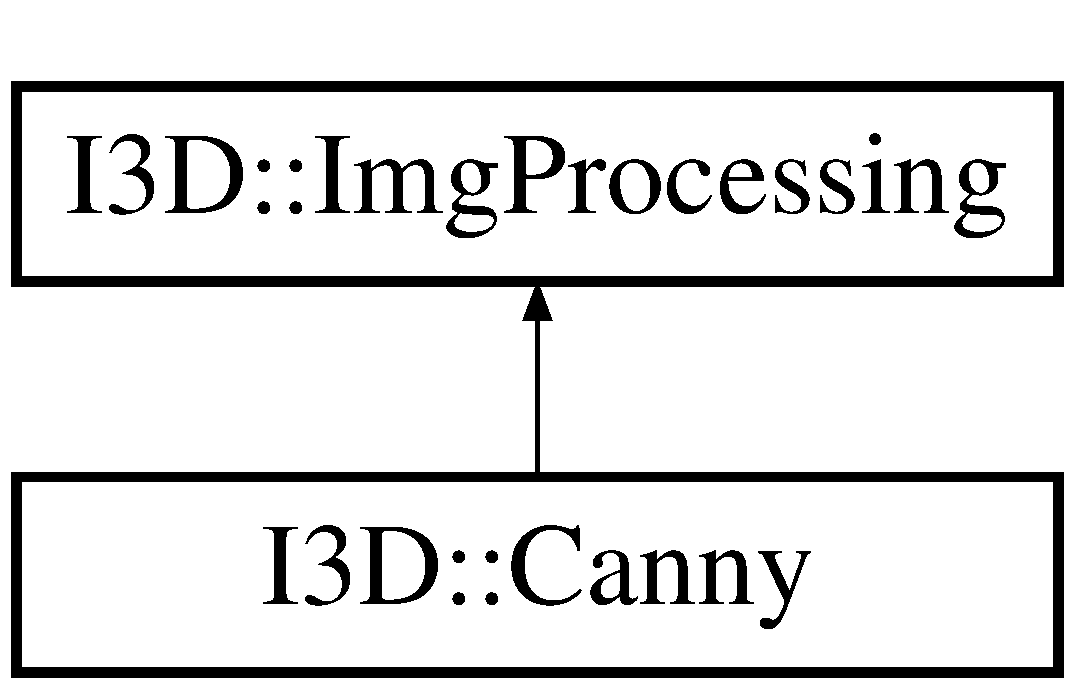
\includegraphics[height=2.000000cm]{class_i3_d_1_1_canny}
\end{center}
\end{figure}
\subsection*{Métodos públicos}
\begin{DoxyCompactItemize}
\item 
\hyperlink{class_i3_d_1_1_canny_a9dd626da444b5d71b001b458081f6af7}{Canny} (double threshold1=0.\+0, double threshold2=0.\+0)
\begin{DoxyCompactList}\small\item\em Constructora. \end{DoxyCompactList}\item 
int \hyperlink{class_i3_d_1_1_canny_a5337ec2dd0c95fe7c9d05444ed8f6425}{execute} (const cv\+::\+Mat \&mat\+In, cv\+::\+Mat $\ast$mat\+Out) const  override
\begin{DoxyCompactList}\small\item\em Ejecuta el proceso. \end{DoxyCompactList}\item 
void \hyperlink{class_i3_d_1_1_canny_afb3f99083d17f060fe791e8498a7d4a7}{set\+Parameters} (double threshold1, double threshold2)
\begin{DoxyCompactList}\small\item\em Establece los parámetros para el detector de bordes canny. \end{DoxyCompactList}\end{DoxyCompactItemize}
\subsection*{Otros miembros heredados}


\subsection{Descripción detallada}
Detector de bordes canny. 

\subsection{Documentación del constructor y destructor}
\index{I3\+D\+::\+Canny@{I3\+D\+::\+Canny}!Canny@{Canny}}
\index{Canny@{Canny}!I3\+D\+::\+Canny@{I3\+D\+::\+Canny}}
\subsubsection[{\texorpdfstring{Canny(double threshold1=0.\+0, double threshold2=0.\+0)}{Canny(double threshold1=0.0, double threshold2=0.0)}}]{\setlength{\rightskip}{0pt plus 5cm}I3\+D\+::\+Canny\+::\+Canny (
\begin{DoxyParamCaption}
\item[{double}]{threshold1 = {\ttfamily 0.0}, }
\item[{double}]{threshold2 = {\ttfamily 0.0}}
\end{DoxyParamCaption}
)\hspace{0.3cm}{\ttfamily [inline]}}\hypertarget{class_i3_d_1_1_canny_a9dd626da444b5d71b001b458081f6af7}{}\label{class_i3_d_1_1_canny_a9dd626da444b5d71b001b458081f6af7}


Constructora. 


\begin{DoxyParams}[1]{Parámetros}
\mbox{\tt in}  & {\em threshold1} & \\
\hline
\mbox{\tt in}  & {\em threshold2} & \\
\hline
\end{DoxyParams}


\subsection{Documentación de las funciones miembro}
\index{I3\+D\+::\+Canny@{I3\+D\+::\+Canny}!execute@{execute}}
\index{execute@{execute}!I3\+D\+::\+Canny@{I3\+D\+::\+Canny}}
\subsubsection[{\texorpdfstring{execute(const cv\+::\+Mat \&mat\+In, cv\+::\+Mat $\ast$mat\+Out) const  override}{execute(const cv::Mat &matIn, cv::Mat *matOut) const  override}}]{\setlength{\rightskip}{0pt plus 5cm}int I3\+D\+::\+Canny\+::execute (
\begin{DoxyParamCaption}
\item[{const cv\+::\+Mat \&}]{mat\+In, }
\item[{cv\+::\+Mat $\ast$}]{mat\+Out}
\end{DoxyParamCaption}
) const\hspace{0.3cm}{\ttfamily [override]}, {\ttfamily [virtual]}}\hypertarget{class_i3_d_1_1_canny_a5337ec2dd0c95fe7c9d05444ed8f6425}{}\label{class_i3_d_1_1_canny_a5337ec2dd0c95fe7c9d05444ed8f6425}


Ejecuta el proceso. 


\begin{DoxyParams}[1]{Parámetros}
\mbox{\tt in}  & {\em mat\+In} & Imagen de entrada \\
\hline
\mbox{\tt out}  & {\em mat\+Out} & Imagen de salida \\
\hline
\end{DoxyParams}
\begin{DoxyReturn}{Devuelve}
Error. Si los procesos se ejecutan correctamente devuelve 0. 
\end{DoxyReturn}


Implementa \hyperlink{class_i3_d_1_1_img_processing_a74195f05bbf034566e9ff6e10f3af4c9}{I3\+D\+::\+Img\+Processing}.

\index{I3\+D\+::\+Canny@{I3\+D\+::\+Canny}!set\+Parameters@{set\+Parameters}}
\index{set\+Parameters@{set\+Parameters}!I3\+D\+::\+Canny@{I3\+D\+::\+Canny}}
\subsubsection[{\texorpdfstring{set\+Parameters(double threshold1, double threshold2)}{setParameters(double threshold1, double threshold2)}}]{\setlength{\rightskip}{0pt plus 5cm}void I3\+D\+::\+Canny\+::set\+Parameters (
\begin{DoxyParamCaption}
\item[{double}]{threshold1, }
\item[{double}]{threshold2}
\end{DoxyParamCaption}
)}\hypertarget{class_i3_d_1_1_canny_afb3f99083d17f060fe791e8498a7d4a7}{}\label{class_i3_d_1_1_canny_afb3f99083d17f060fe791e8498a7d4a7}


Establece los parámetros para el detector de bordes canny. 


\begin{DoxyParams}[1]{Parámetros}
\mbox{\tt in}  & {\em threshold1} & Primer umbral para el procedimiento de histéresis \\
\hline
\mbox{\tt in}  & {\em threshold2} & Segundo umbral para el procedimiento de histéresis \\
\hline
\end{DoxyParams}


La documentación para esta clase fue generada a partir de los siguientes ficheros\+:\begin{DoxyCompactItemize}
\item 
C\+:/\+Desarrollo/tidop/src/\hyperlink{_img_processing_8h}{Img\+Processing.\+h}\item 
C\+:/\+Desarrollo/tidop/src/\hyperlink{_img_processing_8cpp}{Img\+Processing.\+cpp}\end{DoxyCompactItemize}

\hypertarget{class_i3_d_1_1_closing}{}\section{Referencia de la Clase I3D\+:\+:Closing}
\label{class_i3_d_1_1_closing}\index{I3\+D\+::\+Closing@{I3\+D\+::\+Closing}}


Operación morfológica de apertura Esta operación consite en aplicar una dilatación de la imagen seguida de una erosión.  




{\ttfamily \#include $<$Img\+Processing.\+h$>$}

Diagrama de herencias de I3D\+:\+:Closing\begin{figure}[H]
\begin{center}
\leavevmode
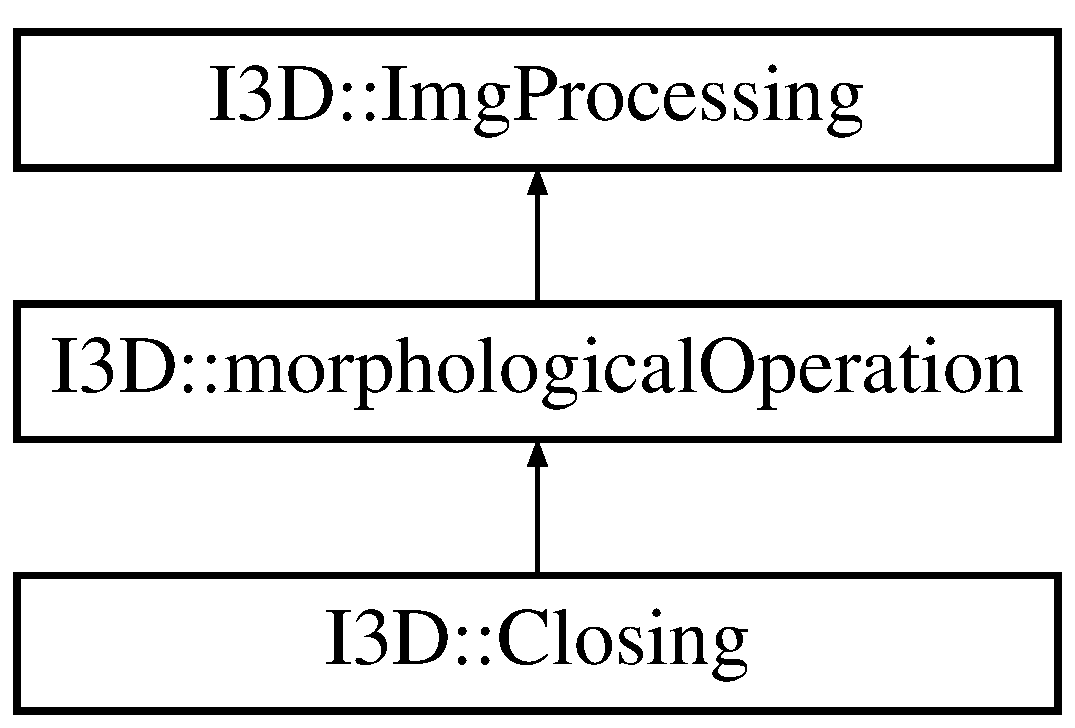
\includegraphics[height=3.000000cm]{class_i3_d_1_1_closing}
\end{center}
\end{figure}
\subsection*{Métodos públicos}
\begin{DoxyCompactItemize}
\item 
\hyperlink{class_i3_d_1_1_closing_a4e5f0f4666d8f1ff8a41abf7da1656f4}{Closing} (int size, cv\+::\+Morph\+Shapes shapes=cv\+::\+M\+O\+R\+P\+H\+\_\+\+R\+E\+CT, cv\+::\+Point anchor=cv\+::\+Point(-\/1,-\/1), int iterations=1, int border\+Type=cv\+::\+B\+O\+R\+D\+E\+R\+\_\+\+C\+O\+N\+S\+T\+A\+NT, const cv\+::\+Scalar \&border\+Value=cv\+::morphology\+Default\+Border\+Value())
\begin{DoxyCompactList}\small\item\em Constructora clase \hyperlink{class_i3_d_1_1_closing}{Closing}. \end{DoxyCompactList}\end{DoxyCompactItemize}
\subsection*{Otros miembros heredados}


\subsection{Descripción detallada}
Operación morfológica de apertura Esta operación consite en aplicar una dilatación de la imagen seguida de una erosión. 

\subsection{Documentación del constructor y destructor}
\index{I3\+D\+::\+Closing@{I3\+D\+::\+Closing}!Closing@{Closing}}
\index{Closing@{Closing}!I3\+D\+::\+Closing@{I3\+D\+::\+Closing}}
\subsubsection[{\texorpdfstring{Closing(int size, cv\+::\+Morph\+Shapes shapes=cv\+::\+M\+O\+R\+P\+H\+\_\+\+R\+E\+C\+T, cv\+::\+Point anchor=cv\+::\+Point(-\/1,-\/1), int iterations=1, int border\+Type=cv\+::\+B\+O\+R\+D\+E\+R\+\_\+\+C\+O\+N\+S\+T\+A\+N\+T, const cv\+::\+Scalar \&border\+Value=cv\+::morphology\+Default\+Border\+Value())}{Closing(int size, cv::MorphShapes shapes=cv::MORPH_RECT, cv::Point anchor=cv::Point(-1,-1), int iterations=1, int borderType=cv::BORDER_CONSTANT, const cv::Scalar &borderValue=cv::morphologyDefaultBorderValue())}}]{\setlength{\rightskip}{0pt plus 5cm}I3\+D\+::\+Closing\+::\+Closing (
\begin{DoxyParamCaption}
\item[{int}]{size, }
\item[{cv\+::\+Morph\+Shapes}]{shapes = {\ttfamily cv\+:\+:MORPH\+\_\+RECT}, }
\item[{cv\+::\+Point}]{anchor = {\ttfamily cv\+:\+:Point(-\/1,~-\/1)}, }
\item[{int}]{iterations = {\ttfamily 1}, }
\item[{int}]{border\+Type = {\ttfamily cv\+:\+:BORDER\+\_\+CONSTANT}, }
\item[{const cv\+::\+Scalar \&}]{border\+Value = {\ttfamily cv\+:\+:morphologyDefaultBorderValue()}}
\end{DoxyParamCaption}
)\hspace{0.3cm}{\ttfamily [inline]}}\hypertarget{class_i3_d_1_1_closing_a4e5f0f4666d8f1ff8a41abf7da1656f4}{}\label{class_i3_d_1_1_closing_a4e5f0f4666d8f1ff8a41abf7da1656f4}


Constructora clase \hyperlink{class_i3_d_1_1_closing}{Closing}. 


\begin{DoxyParams}[1]{Parámetros}
\mbox{\tt in}  & {\em size} & \\
\hline
\mbox{\tt in}  & {\em type} & \\
\hline
\mbox{\tt in}  & {\em anchor} & Punto de anclaje. Por defecto es el centro del kernel \\
\hline
\mbox{\tt in}  & {\em iterations} & \\
\hline
\mbox{\tt in}  & {\em border\+Type} & Método de extrapolación \\
\hline
\mbox{\tt in}  & {\em border\+Value} & \\
\hline
\end{DoxyParams}


La documentación para esta clase fue generada a partir del siguiente fichero\+:\begin{DoxyCompactItemize}
\item 
D\+:/\+Desarrollo/tidop/src/\hyperlink{_img_processing_8h}{Img\+Processing.\+h}\end{DoxyCompactItemize}

\hypertarget{class_i3_d_1_1_dilate}{}\section{Referencia de la Clase I3D\+:\+:Dilate}
\label{class_i3_d_1_1_dilate}\index{I3\+D\+::\+Dilate@{I3\+D\+::\+Dilate}}


Operacion morfologica de dilatación.  




{\ttfamily \#include $<$Img\+Processing.\+h$>$}

Diagrama de herencias de I3D\+:\+:Dilate\begin{figure}[H]
\begin{center}
\leavevmode
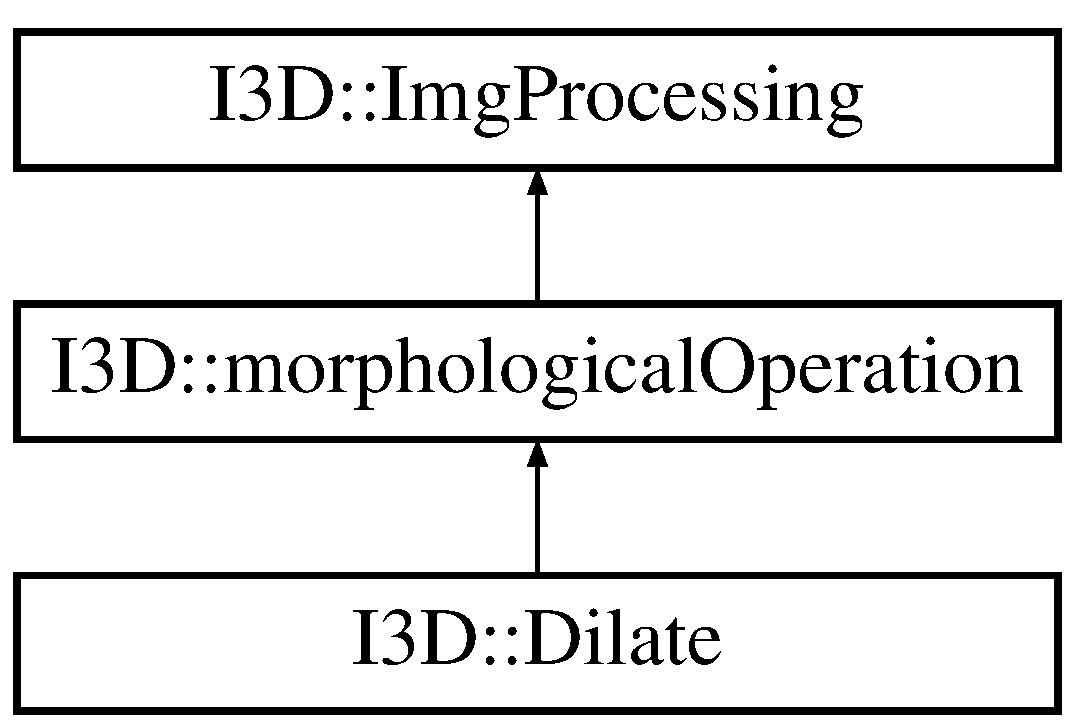
\includegraphics[height=3.000000cm]{class_i3_d_1_1_dilate}
\end{center}
\end{figure}
\subsection*{Métodos públicos}
\begin{DoxyCompactItemize}
\item 
\hyperlink{class_i3_d_1_1_dilate_a6b44ace9b52b4eab5da68d574e4ad7f1}{Dilate} (int size, cv\+::\+Morph\+Shapes shapes=cv\+::\+M\+O\+R\+P\+H\+\_\+\+R\+E\+CT, cv\+::\+Point anchor=cv\+::\+Point(-\/1,-\/1), int iterations=1, int border\+Type=cv\+::\+B\+O\+R\+D\+E\+R\+\_\+\+C\+O\+N\+S\+T\+A\+NT, const cv\+::\+Scalar \&border\+Value=cv\+::morphology\+Default\+Border\+Value())
\begin{DoxyCompactList}\small\item\em Constructora. \end{DoxyCompactList}\end{DoxyCompactItemize}
\subsection*{Otros miembros heredados}


\subsection{Descripción detallada}
Operacion morfologica de dilatación. 

\subsection{Documentación del constructor y destructor}
\index{I3\+D\+::\+Dilate@{I3\+D\+::\+Dilate}!Dilate@{Dilate}}
\index{Dilate@{Dilate}!I3\+D\+::\+Dilate@{I3\+D\+::\+Dilate}}
\subsubsection[{\texorpdfstring{Dilate(int size, cv\+::\+Morph\+Shapes shapes=cv\+::\+M\+O\+R\+P\+H\+\_\+\+R\+E\+C\+T, cv\+::\+Point anchor=cv\+::\+Point(-\/1,-\/1), int iterations=1, int border\+Type=cv\+::\+B\+O\+R\+D\+E\+R\+\_\+\+C\+O\+N\+S\+T\+A\+N\+T, const cv\+::\+Scalar \&border\+Value=cv\+::morphology\+Default\+Border\+Value())}{Dilate(int size, cv::MorphShapes shapes=cv::MORPH_RECT, cv::Point anchor=cv::Point(-1,-1), int iterations=1, int borderType=cv::BORDER_CONSTANT, const cv::Scalar &borderValue=cv::morphologyDefaultBorderValue())}}]{\setlength{\rightskip}{0pt plus 5cm}I3\+D\+::\+Dilate\+::\+Dilate (
\begin{DoxyParamCaption}
\item[{int}]{size, }
\item[{cv\+::\+Morph\+Shapes}]{shapes = {\ttfamily cv\+:\+:MORPH\+\_\+RECT}, }
\item[{cv\+::\+Point}]{anchor = {\ttfamily cv\+:\+:Point(-\/1,~-\/1)}, }
\item[{int}]{iterations = {\ttfamily 1}, }
\item[{int}]{border\+Type = {\ttfamily cv\+:\+:BORDER\+\_\+CONSTANT}, }
\item[{const cv\+::\+Scalar \&}]{border\+Value = {\ttfamily cv\+:\+:morphologyDefaultBorderValue()}}
\end{DoxyParamCaption}
)\hspace{0.3cm}{\ttfamily [inline]}}\hypertarget{class_i3_d_1_1_dilate_a6b44ace9b52b4eab5da68d574e4ad7f1}{}\label{class_i3_d_1_1_dilate_a6b44ace9b52b4eab5da68d574e4ad7f1}


Constructora. 


\begin{DoxyParams}[1]{Parámetros}
\mbox{\tt in}  & {\em size} & \\
\hline
\mbox{\tt in}  & {\em type} & \\
\hline
\mbox{\tt in}  & {\em anchor} & Punto de anclaje. Por defecto es el centro del kernel \\
\hline
\mbox{\tt in}  & {\em iterations} & \\
\hline
\mbox{\tt in}  & {\em border\+Type} & Método de extrapolación \\
\hline
\mbox{\tt in}  & {\em border\+Value} & \\
\hline
\end{DoxyParams}


La documentación para esta clase fue generada a partir del siguiente fichero\+:\begin{DoxyCompactItemize}
\item 
C\+:/\+Desarrollo/tidop/src/\hyperlink{_img_processing_8h}{Img\+Processing.\+h}\end{DoxyCompactItemize}

\hypertarget{class_i3_d_1_1_discrete_fourier_trf}{}\section{Referencia de la Clase I3D\+:\+:Discrete\+Fourier\+Trf}
\label{class_i3_d_1_1_discrete_fourier_trf}\index{I3\+D\+::\+Discrete\+Fourier\+Trf@{I3\+D\+::\+Discrete\+Fourier\+Trf}}


The Fourier class Discrete Fourier \hyperlink{class_i3_d_1_1_transform}{Transform}.  




{\ttfamily \#include $<$fourier.\+h$>$}

\subsection*{Métodos públicos}
\begin{DoxyCompactItemize}
\item 
\hyperlink{class_i3_d_1_1_discrete_fourier_trf_af2a71fc09dd90202fde0c7681d60843c}{Discrete\+Fourier\+Trf} ()
\begin{DoxyCompactList}\small\item\em Constuctora transformada discreta de Fourier. \end{DoxyCompactList}\item 
void \hyperlink{class_i3_d_1_1_discrete_fourier_trf_a75654523e5a83d416e5aa2caa575bb69}{forward} (const cv\+::\+Mat \&source, cv\+::\+Mat $\ast$out) const 
\begin{DoxyCompactList}\small\item\em Transformación directa. \end{DoxyCompactList}\item 
void \hyperlink{class_i3_d_1_1_discrete_fourier_trf_aa6f6a2e71d2dc2b5b3beca65913416a0}{inverse} (const cv\+::\+Mat \&source, cv\+::\+Mat $\ast$out) const 
\begin{DoxyCompactList}\small\item\em Transformación inversa. \end{DoxyCompactList}\item 
void \hyperlink{class_i3_d_1_1_discrete_fourier_trf_ae9a5042d59d049325adc7fcc046b7a0e}{shift} (cv\+::\+Mat \&image) const 
\begin{DoxyCompactList}\small\item\em Intercambia los cuadrantes. \end{DoxyCompactList}\end{DoxyCompactItemize}


\subsection{Descripción detallada}
The Fourier class Discrete Fourier \hyperlink{class_i3_d_1_1_transform}{Transform}. 

\subsection{Documentación del constructor y destructor}
\index{I3\+D\+::\+Discrete\+Fourier\+Trf@{I3\+D\+::\+Discrete\+Fourier\+Trf}!Discrete\+Fourier\+Trf@{Discrete\+Fourier\+Trf}}
\index{Discrete\+Fourier\+Trf@{Discrete\+Fourier\+Trf}!I3\+D\+::\+Discrete\+Fourier\+Trf@{I3\+D\+::\+Discrete\+Fourier\+Trf}}
\subsubsection[{\texorpdfstring{Discrete\+Fourier\+Trf()}{DiscreteFourierTrf()}}]{\setlength{\rightskip}{0pt plus 5cm}I3\+D\+::\+Discrete\+Fourier\+Trf\+::\+Discrete\+Fourier\+Trf (
\begin{DoxyParamCaption}
{}
\end{DoxyParamCaption}
)\hspace{0.3cm}{\ttfamily [inline]}}\hypertarget{class_i3_d_1_1_discrete_fourier_trf_af2a71fc09dd90202fde0c7681d60843c}{}\label{class_i3_d_1_1_discrete_fourier_trf_af2a71fc09dd90202fde0c7681d60843c}


Constuctora transformada discreta de Fourier. 



\subsection{Documentación de las funciones miembro}
\index{I3\+D\+::\+Discrete\+Fourier\+Trf@{I3\+D\+::\+Discrete\+Fourier\+Trf}!forward@{forward}}
\index{forward@{forward}!I3\+D\+::\+Discrete\+Fourier\+Trf@{I3\+D\+::\+Discrete\+Fourier\+Trf}}
\subsubsection[{\texorpdfstring{forward(const cv\+::\+Mat \&source, cv\+::\+Mat $\ast$out) const }{forward(const cv::Mat &source, cv::Mat *out) const }}]{\setlength{\rightskip}{0pt plus 5cm}void I3\+D\+::\+Discrete\+Fourier\+Trf\+::forward (
\begin{DoxyParamCaption}
\item[{const cv\+::\+Mat \&}]{source, }
\item[{cv\+::\+Mat $\ast$}]{out}
\end{DoxyParamCaption}
) const}\hypertarget{class_i3_d_1_1_discrete_fourier_trf_a75654523e5a83d416e5aa2caa575bb69}{}\label{class_i3_d_1_1_discrete_fourier_trf_a75654523e5a83d416e5aa2caa575bb69}


Transformación directa. 


\begin{DoxyParams}[1]{Parámetros}
\mbox{\tt in}  & {\em source} & Imagen de entrada \\
\hline
\mbox{\tt out}  & {\em out} & Imagen de salida \\
\hline
\end{DoxyParams}
\index{I3\+D\+::\+Discrete\+Fourier\+Trf@{I3\+D\+::\+Discrete\+Fourier\+Trf}!inverse@{inverse}}
\index{inverse@{inverse}!I3\+D\+::\+Discrete\+Fourier\+Trf@{I3\+D\+::\+Discrete\+Fourier\+Trf}}
\subsubsection[{\texorpdfstring{inverse(const cv\+::\+Mat \&source, cv\+::\+Mat $\ast$out) const }{inverse(const cv::Mat &source, cv::Mat *out) const }}]{\setlength{\rightskip}{0pt plus 5cm}void I3\+D\+::\+Discrete\+Fourier\+Trf\+::inverse (
\begin{DoxyParamCaption}
\item[{const cv\+::\+Mat \&}]{source, }
\item[{cv\+::\+Mat $\ast$}]{out}
\end{DoxyParamCaption}
) const}\hypertarget{class_i3_d_1_1_discrete_fourier_trf_aa6f6a2e71d2dc2b5b3beca65913416a0}{}\label{class_i3_d_1_1_discrete_fourier_trf_aa6f6a2e71d2dc2b5b3beca65913416a0}


Transformación inversa. 


\begin{DoxyParams}[1]{Parámetros}
\mbox{\tt in}  & {\em source} & Imagen de entrada \\
\hline
\mbox{\tt out}  & {\em out} & Imagen de salida \\
\hline
\end{DoxyParams}
\index{I3\+D\+::\+Discrete\+Fourier\+Trf@{I3\+D\+::\+Discrete\+Fourier\+Trf}!shift@{shift}}
\index{shift@{shift}!I3\+D\+::\+Discrete\+Fourier\+Trf@{I3\+D\+::\+Discrete\+Fourier\+Trf}}
\subsubsection[{\texorpdfstring{shift(cv\+::\+Mat \&image) const }{shift(cv::Mat &image) const }}]{\setlength{\rightskip}{0pt plus 5cm}void I3\+D\+::\+Discrete\+Fourier\+Trf\+::shift (
\begin{DoxyParamCaption}
\item[{cv\+::\+Mat \&}]{image}
\end{DoxyParamCaption}
) const}\hypertarget{class_i3_d_1_1_discrete_fourier_trf_ae9a5042d59d049325adc7fcc046b7a0e}{}\label{class_i3_d_1_1_discrete_fourier_trf_ae9a5042d59d049325adc7fcc046b7a0e}


Intercambia los cuadrantes. 


\begin{DoxyParams}[1]{Parámetros}
\mbox{\tt in}  & {\em image} & \\
\hline
\end{DoxyParams}


La documentación para esta clase fue generada a partir de los siguientes ficheros\+:\begin{DoxyCompactItemize}
\item 
C\+:/\+Desarrollo/tidop/src/\hyperlink{fourier_8h}{fourier.\+h}\item 
C\+:/\+Desarrollo/tidop/src/\hyperlink{fourier_8cpp}{fourier.\+cpp}\end{DoxyCompactItemize}

\hypertarget{class_i3_d_1_1_equalize_histogram}{}\section{Referencia de la Clase I3D\+:\+:Equalize\+Histogram}
\label{class_i3_d_1_1_equalize_histogram}\index{I3\+D\+::\+Equalize\+Histogram@{I3\+D\+::\+Equalize\+Histogram}}


Ecualización del histograma. Mejora del contraste de la imagen mediante la ecualización del histograma.  




{\ttfamily \#include $<$Img\+Processing.\+h$>$}

Diagrama de herencias de I3D\+:\+:Equalize\+Histogram\begin{figure}[H]
\begin{center}
\leavevmode
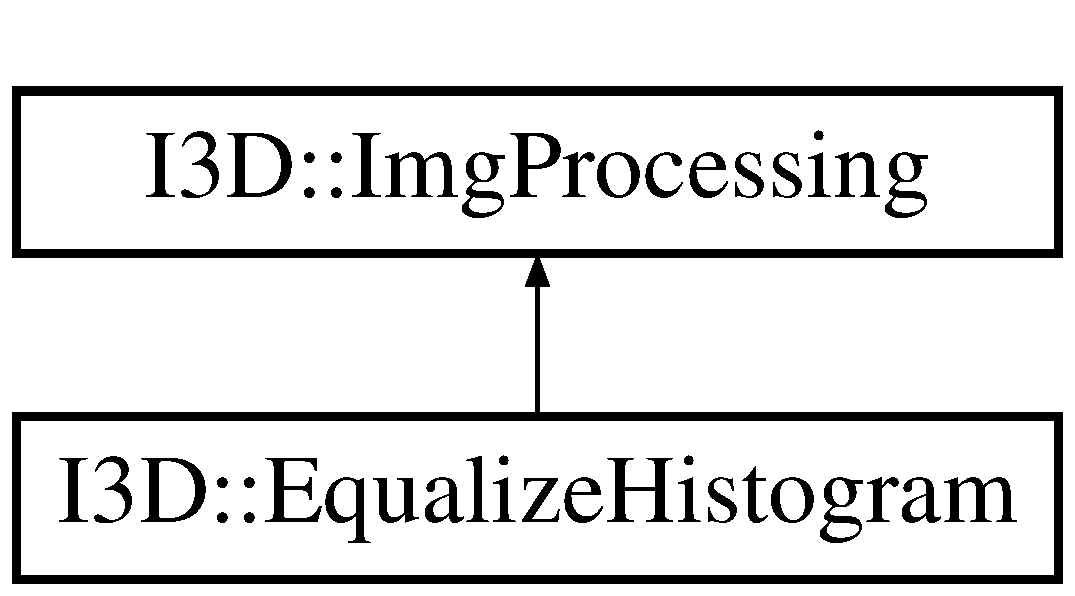
\includegraphics[height=2.000000cm]{class_i3_d_1_1_equalize_histogram}
\end{center}
\end{figure}
\subsection*{Métodos públicos}
\begin{DoxyCompactItemize}
\item 
\hyperlink{class_i3_d_1_1_equalize_histogram_afd85554f82ab1fe8b0ded39fd181012d}{Equalize\+Histogram} ()
\begin{DoxyCompactList}\small\item\em Constructora de la clase. \end{DoxyCompactList}\item 
int \hyperlink{class_i3_d_1_1_equalize_histogram_ac748887f28d189287a120b5c6b0977a2}{execute} (const cv\+::\+Mat \&mat\+In, cv\+::\+Mat $\ast$mat\+Out) const  override
\begin{DoxyCompactList}\small\item\em Ejecuta el proceso. \end{DoxyCompactList}\end{DoxyCompactItemize}
\subsection*{Otros miembros heredados}


\subsection{Descripción detallada}
Ecualización del histograma. Mejora del contraste de la imagen mediante la ecualización del histograma. 

\subsection{Documentación del constructor y destructor}
\index{I3\+D\+::\+Equalize\+Histogram@{I3\+D\+::\+Equalize\+Histogram}!Equalize\+Histogram@{Equalize\+Histogram}}
\index{Equalize\+Histogram@{Equalize\+Histogram}!I3\+D\+::\+Equalize\+Histogram@{I3\+D\+::\+Equalize\+Histogram}}
\subsubsection[{\texorpdfstring{Equalize\+Histogram()}{EqualizeHistogram()}}]{\setlength{\rightskip}{0pt plus 5cm}I3\+D\+::\+Equalize\+Histogram\+::\+Equalize\+Histogram (
\begin{DoxyParamCaption}
{}
\end{DoxyParamCaption}
)\hspace{0.3cm}{\ttfamily [inline]}}\hypertarget{class_i3_d_1_1_equalize_histogram_afd85554f82ab1fe8b0ded39fd181012d}{}\label{class_i3_d_1_1_equalize_histogram_afd85554f82ab1fe8b0ded39fd181012d}


Constructora de la clase. 



\subsection{Documentación de las funciones miembro}
\index{I3\+D\+::\+Equalize\+Histogram@{I3\+D\+::\+Equalize\+Histogram}!execute@{execute}}
\index{execute@{execute}!I3\+D\+::\+Equalize\+Histogram@{I3\+D\+::\+Equalize\+Histogram}}
\subsubsection[{\texorpdfstring{execute(const cv\+::\+Mat \&mat\+In, cv\+::\+Mat $\ast$mat\+Out) const  override}{execute(const cv::Mat &matIn, cv::Mat *matOut) const  override}}]{\setlength{\rightskip}{0pt plus 5cm}int I3\+D\+::\+Equalize\+Histogram\+::execute (
\begin{DoxyParamCaption}
\item[{const cv\+::\+Mat \&}]{mat\+In, }
\item[{cv\+::\+Mat $\ast$}]{mat\+Out}
\end{DoxyParamCaption}
) const\hspace{0.3cm}{\ttfamily [override]}, {\ttfamily [virtual]}}\hypertarget{class_i3_d_1_1_equalize_histogram_ac748887f28d189287a120b5c6b0977a2}{}\label{class_i3_d_1_1_equalize_histogram_ac748887f28d189287a120b5c6b0977a2}


Ejecuta el proceso. 


\begin{DoxyParams}[1]{Parámetros}
\mbox{\tt in}  & {\em mat\+In} & Imagen de entrada. \\
\hline
\mbox{\tt out}  & {\em mat\+Out} & Imagen de salida. \\
\hline
\end{DoxyParams}
\begin{DoxyReturn}{Devuelve}
Error. Si los procesos se ejecutan correctamente devuelve 0. 
\end{DoxyReturn}


Implementa \hyperlink{class_i3_d_1_1_img_processing_a74195f05bbf034566e9ff6e10f3af4c9}{I3\+D\+::\+Img\+Processing}.



La documentación para esta clase fue generada a partir de los siguientes ficheros\+:\begin{DoxyCompactItemize}
\item 
D\+:/\+Desarrollo/tidop/src/\hyperlink{_img_processing_8h}{Img\+Processing.\+h}\item 
D\+:/\+Desarrollo/tidop/src/\hyperlink{_img_processing_8cpp}{Img\+Processing.\+cpp}\end{DoxyCompactItemize}

\hypertarget{class_i3_d_1_1_erotion}{}\section{Referencia de la Clase I3D\+:\+:Erotion}
\label{class_i3_d_1_1_erotion}\index{I3\+D\+::\+Erotion@{I3\+D\+::\+Erotion}}


Operacion morfologica de erosión.  




{\ttfamily \#include $<$Img\+Processing.\+h$>$}

Diagrama de herencias de I3D\+:\+:Erotion\begin{figure}[H]
\begin{center}
\leavevmode
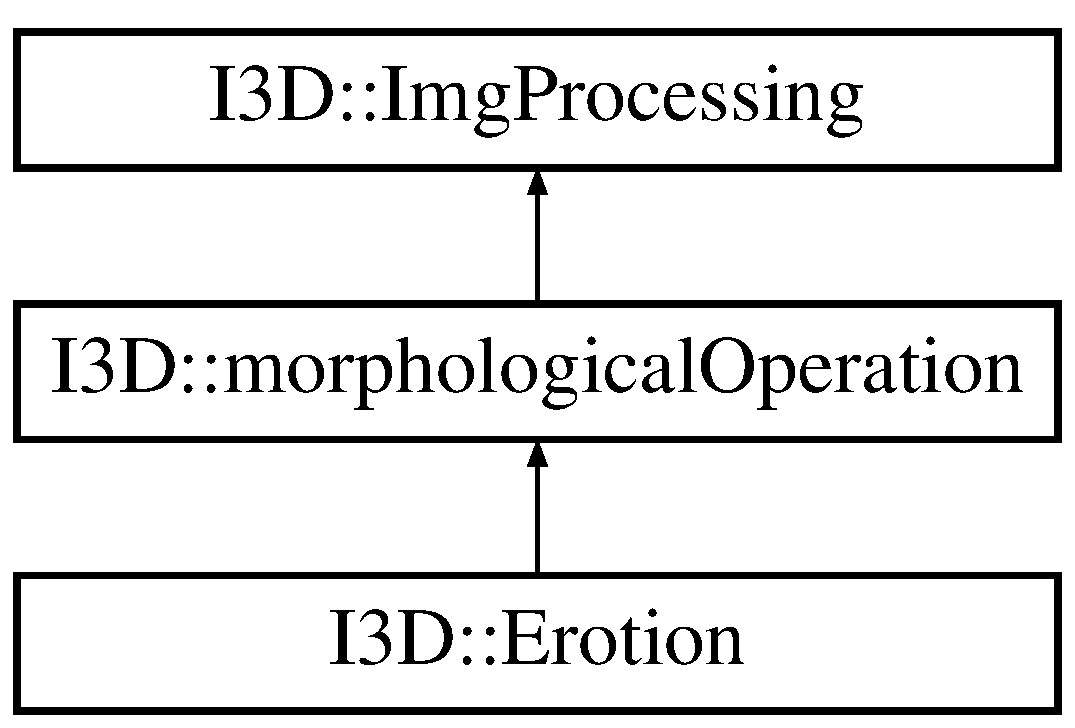
\includegraphics[height=3.000000cm]{class_i3_d_1_1_erotion}
\end{center}
\end{figure}
\subsection*{Métodos públicos}
\begin{DoxyCompactItemize}
\item 
\hyperlink{class_i3_d_1_1_erotion_a522346abdebbcf2d634aac7d9375ecce}{Erotion} (int size, cv\+::\+Morph\+Shapes shapes=cv\+::\+M\+O\+R\+P\+H\+\_\+\+R\+E\+CT, cv\+::\+Point anchor=cv\+::\+Point(-\/1,-\/1), int iterations=1, int border\+Type=cv\+::\+B\+O\+R\+D\+E\+R\+\_\+\+C\+O\+N\+S\+T\+A\+NT, const cv\+::\+Scalar \&border\+Value=cv\+::morphology\+Default\+Border\+Value())
\begin{DoxyCompactList}\small\item\em Constructora clase \hyperlink{class_i3_d_1_1_erotion}{Erotion}. \end{DoxyCompactList}\end{DoxyCompactItemize}
\subsection*{Otros miembros heredados}


\subsection{Descripción detallada}
Operacion morfologica de erosión. 

\subsection{Documentación del constructor y destructor}
\index{I3\+D\+::\+Erotion@{I3\+D\+::\+Erotion}!Erotion@{Erotion}}
\index{Erotion@{Erotion}!I3\+D\+::\+Erotion@{I3\+D\+::\+Erotion}}
\subsubsection[{\texorpdfstring{Erotion(int size, cv\+::\+Morph\+Shapes shapes=cv\+::\+M\+O\+R\+P\+H\+\_\+\+R\+E\+C\+T, cv\+::\+Point anchor=cv\+::\+Point(-\/1,-\/1), int iterations=1, int border\+Type=cv\+::\+B\+O\+R\+D\+E\+R\+\_\+\+C\+O\+N\+S\+T\+A\+N\+T, const cv\+::\+Scalar \&border\+Value=cv\+::morphology\+Default\+Border\+Value())}{Erotion(int size, cv::MorphShapes shapes=cv::MORPH_RECT, cv::Point anchor=cv::Point(-1,-1), int iterations=1, int borderType=cv::BORDER_CONSTANT, const cv::Scalar &borderValue=cv::morphologyDefaultBorderValue())}}]{\setlength{\rightskip}{0pt plus 5cm}I3\+D\+::\+Erotion\+::\+Erotion (
\begin{DoxyParamCaption}
\item[{int}]{size, }
\item[{cv\+::\+Morph\+Shapes}]{shapes = {\ttfamily cv\+:\+:MORPH\+\_\+RECT}, }
\item[{cv\+::\+Point}]{anchor = {\ttfamily cv\+:\+:Point(-\/1,~-\/1)}, }
\item[{int}]{iterations = {\ttfamily 1}, }
\item[{int}]{border\+Type = {\ttfamily cv\+:\+:BORDER\+\_\+CONSTANT}, }
\item[{const cv\+::\+Scalar \&}]{border\+Value = {\ttfamily cv\+:\+:morphologyDefaultBorderValue()}}
\end{DoxyParamCaption}
)\hspace{0.3cm}{\ttfamily [inline]}}\hypertarget{class_i3_d_1_1_erotion_a522346abdebbcf2d634aac7d9375ecce}{}\label{class_i3_d_1_1_erotion_a522346abdebbcf2d634aac7d9375ecce}


Constructora clase \hyperlink{class_i3_d_1_1_erotion}{Erotion}. 


\begin{DoxyParams}[1]{Parámetros}
\mbox{\tt in}  & {\em size} & \\
\hline
\mbox{\tt in}  & {\em type} & \\
\hline
\mbox{\tt in}  & {\em anchor} & Punto de anclaje. Por defecto es el centro del kernel \\
\hline
\mbox{\tt in}  & {\em iterations} & \\
\hline
\mbox{\tt in}  & {\em border\+Type} & Método de extrapolación \\
\hline
\mbox{\tt in}  & {\em border\+Value} & \\
\hline
\end{DoxyParams}


La documentación para esta clase fue generada a partir del siguiente fichero\+:\begin{DoxyCompactItemize}
\item 
C\+:/\+Desarrollo/tidop/src/\hyperlink{_img_processing_8h}{Img\+Processing.\+h}\end{DoxyCompactItemize}

\hypertarget{class_i3_d_1_1_features2_d}{}\section{Referencia de la Clase I3D\+:\+:Features2D}
\label{class_i3_d_1_1_features2_d}\index{I3\+D\+::\+Features2D@{I3\+D\+::\+Features2D}}


The \hyperlink{class_i3_d_1_1_features2_d}{Features2D} class.  




{\ttfamily \#include $<$matching.\+h$>$}

\subsection*{Métodos públicos}
\begin{DoxyCompactItemize}
\item 
\hyperlink{class_i3_d_1_1_features2_d_a14b2aca15beaeb0bf20874246022bdf3}{Features2D} ()
\begin{DoxyCompactList}\small\item\em Constructora por defecto \hyperlink{class_i3_d_1_1_features2_d}{Features2D}. \end{DoxyCompactList}\item 
\hyperlink{class_i3_d_1_1_features2_d_a0daae1513e7dfdeb6fbed6f188a0ffb6}{Features2D} (const cv\+::\+Ptr$<$ cv\+::\+Feature\+Detector $>$ \&fd, const cv\+::\+Ptr$<$ cv\+::\+Descriptor\+Extractor $>$ \&de)
\begin{DoxyCompactList}\small\item\em Constructora \hyperlink{class_i3_d_1_1_features2_d}{Features2D} Se le pasan como parametro un detector de caracteristicas y un extractor de descriptores. \end{DoxyCompactList}\item 
\hyperlink{class_i3_d_1_1_features2_d_a0596063dc4934fb9b8768e3dd83f830a}{$\sim$\+Features2D} ()
\begin{DoxyCompactList}\small\item\em Destructora \hyperlink{class_i3_d_1_1_features2_d}{Features2D}. \end{DoxyCompactList}\item 
void \hyperlink{class_i3_d_1_1_features2_d_a7fd78be8b44ca2dcfc8bb30cec1d3743}{set\+Feature\+Detector} (const cv\+::\+Ptr$<$ cv\+::\+Feature\+Detector $>$ \&fd)
\begin{DoxyCompactList}\small\item\em Establece el detector de caracteristicas. \end{DoxyCompactList}\item 
void \hyperlink{class_i3_d_1_1_features2_d_a8c34027b40e0be15923e3d18fe668cdd}{set\+Descriptor\+Extractor} (const cv\+::\+Ptr$<$ cv\+::\+Descriptor\+Extractor $>$ \&de)
\begin{DoxyCompactList}\small\item\em Establece el extractor de descriptores. \end{DoxyCompactList}\item 
int \hyperlink{class_i3_d_1_1_features2_d_a62ecf2a0260a7cc171606038e9dff77f}{detect\+Key\+Points} (const cv\+::\+Mat \&img, std\+::vector$<$ cv\+::\+Key\+Point $>$ $\ast$key\+Points=N\+U\+LL, const cv\+::\+Input\+Array \&mask=cv\+::no\+Array())
\begin{DoxyCompactList}\small\item\em Detect\+Key\+Points. \end{DoxyCompactList}\item 
void \hyperlink{class_i3_d_1_1_features2_d_a5da82180382ed94fc8c197ea7f03911b}{calc\+Descriptor} (const cv\+::\+Mat \&img, std\+::vector$<$ cv\+::\+Key\+Point $>$ $\ast$key\+Points=N\+U\+LL, cv\+::\+Mat $\ast$descriptor=N\+U\+LL)
\begin{DoxyCompactList}\small\item\em Calcula los Descriptores. \end{DoxyCompactList}\item 
void \hyperlink{class_i3_d_1_1_features2_d_a9a6855620abadd6571352d3fbfd29381}{save} (const char $\ast$fname) const 
\begin{DoxyCompactList}\small\item\em Guarda en un fichero los keypoints y los descriptores. \end{DoxyCompactList}\item 
void \hyperlink{class_i3_d_1_1_features2_d_ae999316e0882a9c2a29a29e3e5b5e746}{read} (const char $\ast$fname)
\begin{DoxyCompactList}\small\item\em Lectura de un fichero con los keypoints y descriptores. \end{DoxyCompactList}\item 
const std\+::vector$<$ cv\+::\+Key\+Point $>$ \& \hyperlink{class_i3_d_1_1_features2_d_a5543362d3c3d1f1e0072ac1b8090217a}{get\+Key\+Points} ()
\begin{DoxyCompactList}\small\item\em Devuelve los Key\+Points. \end{DoxyCompactList}\item 
const cv\+::\+Key\+Point \& \hyperlink{class_i3_d_1_1_features2_d_a725ae53258ccfd1b6a9d75646d75bba7}{get\+Key\+Point} (int id) const 
\begin{DoxyCompactList}\small\item\em Devuelve un Key\+Point. \end{DoxyCompactList}\item 
const cv\+::\+Mat \& \hyperlink{class_i3_d_1_1_features2_d_a360185a32ca3b28f9fdd51d4506574e8}{get\+Descriptors} () const 
\begin{DoxyCompactList}\small\item\em Devuelve los descriptores. \end{DoxyCompactList}\item 
{\footnotesize template$<$typename T $>$ }\\void \hyperlink{class_i3_d_1_1_features2_d_a82849d415643f6e8e1c39e3274cade99}{filter} (const cv\+::\+Mat \&in, const \hyperlink{class_i3_d_1_1_window}{Window}$<$ T $>$ \&w, cv\+::\+Mat $\ast$out, std\+::vector$<$ cv\+::\+Key\+Point $>$ $\ast$\+\_\+key\+Points, cv\+::\+Mat $\ast$\+\_\+descriptor)
\begin{DoxyCompactList}\small\item\em Filtrado de keypoints por ventana Los puntos que estén fuera de la ventana se eliminan. \end{DoxyCompactList}\end{DoxyCompactItemize}


\subsection{Descripción detallada}
The \hyperlink{class_i3_d_1_1_features2_d}{Features2D} class. 

\subsection{Documentación del constructor y destructor}
\index{I3\+D\+::\+Features2D@{I3\+D\+::\+Features2D}!Features2D@{Features2D}}
\index{Features2D@{Features2D}!I3\+D\+::\+Features2D@{I3\+D\+::\+Features2D}}
\subsubsection[{\texorpdfstring{Features2\+D()}{Features2D()}}]{\setlength{\rightskip}{0pt plus 5cm}I3\+D\+::\+Features2\+D\+::\+Features2D (
\begin{DoxyParamCaption}
{}
\end{DoxyParamCaption}
)\hspace{0.3cm}{\ttfamily [inline]}}\hypertarget{class_i3_d_1_1_features2_d_a14b2aca15beaeb0bf20874246022bdf3}{}\label{class_i3_d_1_1_features2_d_a14b2aca15beaeb0bf20874246022bdf3}


Constructora por defecto \hyperlink{class_i3_d_1_1_features2_d}{Features2D}. 

\index{I3\+D\+::\+Features2D@{I3\+D\+::\+Features2D}!Features2D@{Features2D}}
\index{Features2D@{Features2D}!I3\+D\+::\+Features2D@{I3\+D\+::\+Features2D}}
\subsubsection[{\texorpdfstring{Features2\+D(const cv\+::\+Ptr$<$ cv\+::\+Feature\+Detector $>$ \&fd, const cv\+::\+Ptr$<$ cv\+::\+Descriptor\+Extractor $>$ \&de)}{Features2D(const cv::Ptr< cv::FeatureDetector > &fd, const cv::Ptr< cv::DescriptorExtractor > &de)}}]{\setlength{\rightskip}{0pt plus 5cm}I3\+D\+::\+Features2\+D\+::\+Features2D (
\begin{DoxyParamCaption}
\item[{const cv\+::\+Ptr$<$ cv\+::\+Feature\+Detector $>$ \&}]{fd, }
\item[{const cv\+::\+Ptr$<$ cv\+::\+Descriptor\+Extractor $>$ \&}]{de}
\end{DoxyParamCaption}
)\hspace{0.3cm}{\ttfamily [inline]}}\hypertarget{class_i3_d_1_1_features2_d_a0daae1513e7dfdeb6fbed6f188a0ffb6}{}\label{class_i3_d_1_1_features2_d_a0daae1513e7dfdeb6fbed6f188a0ffb6}


Constructora \hyperlink{class_i3_d_1_1_features2_d}{Features2D} Se le pasan como parametro un detector de caracteristicas y un extractor de descriptores. 


\begin{DoxyParams}[1]{Parámetros}
\mbox{\tt in}  & {\em \+\_\+fd} & Detector de caracteristicas \\
\hline
\mbox{\tt in}  & {\em \+\_\+de} & Extractor de descriptores\\
\hline
\end{DoxyParams}
Detectores soportados\+:
\begin{DoxyItemize}
\item cv\+::\+Agast\+Feature\+Detector\+::create()
\item cv\+::\+A\+K\+A\+Z\+E\+::create();
\item cv\+::\+B\+R\+I\+S\+K\+::create();
\item cv\+::\+Fast\+Feature\+Detector\+::create();
\item cv\+::\+G\+F\+T\+T\+Detector\+::create();
\item cv\+::\+K\+A\+Z\+E\+::create();
\item cv\+::\+M\+S\+E\+R\+::create();
\item cv\+::\+O\+R\+B\+::create();
\item cv\+::\+Simple\+Blob\+Detector\+::create();
\item cv\+::xfeatures2d\+::\+Brief\+Descriptor\+Extractor\+::create();
\item cv\+::xfeatures2d\+::\+D\+A\+I\+S\+Y\+::create();
\item cv\+::xfeatures2d\+::\+F\+R\+E\+A\+K\+::create();
\item cv\+::xfeatures2d\+::\+L\+A\+T\+C\+H\+::create();
\item cv\+::xfeatures2d\+::\+L\+U\+C\+I\+D\+::create();
\item cv\+::xfeatures2d\+::\+M\+S\+D\+Detector\+::create();
\item cv\+::xfeatures2d\+::\+S\+I\+F\+T\+::create();
\item cv\+::xfeatures2d\+::\+Star\+Detector\+::create();
\item cv\+::xfeatures2d\+::\+S\+U\+R\+F\+::create();
\end{DoxyItemize}

Descriptores\+:
\begin{DoxyItemize}
\item cv\+::\+B\+R\+I\+S\+K\+::create();
\item cv\+::\+O\+R\+B\+::create();
\item cv\+::\+A\+K\+A\+Z\+E\+::create();
\item cv\+::xfeatures2d\+::\+S\+I\+F\+T\+::create();
\item cv\+::xfeatures2d\+::\+S\+U\+R\+F\+::create(); 
\end{DoxyItemize}\index{I3\+D\+::\+Features2D@{I3\+D\+::\+Features2D}!````~Features2D@{$\sim$\+Features2D}}
\index{````~Features2D@{$\sim$\+Features2D}!I3\+D\+::\+Features2D@{I3\+D\+::\+Features2D}}
\subsubsection[{\texorpdfstring{$\sim$\+Features2\+D()}{~Features2D()}}]{\setlength{\rightskip}{0pt plus 5cm}I3\+D\+::\+Features2\+D\+::$\sim$\+Features2D (
\begin{DoxyParamCaption}
{}
\end{DoxyParamCaption}
)}\hypertarget{class_i3_d_1_1_features2_d_a0596063dc4934fb9b8768e3dd83f830a}{}\label{class_i3_d_1_1_features2_d_a0596063dc4934fb9b8768e3dd83f830a}


Destructora \hyperlink{class_i3_d_1_1_features2_d}{Features2D}. 



\subsection{Documentación de las funciones miembro}
\index{I3\+D\+::\+Features2D@{I3\+D\+::\+Features2D}!calc\+Descriptor@{calc\+Descriptor}}
\index{calc\+Descriptor@{calc\+Descriptor}!I3\+D\+::\+Features2D@{I3\+D\+::\+Features2D}}
\subsubsection[{\texorpdfstring{calc\+Descriptor(const cv\+::\+Mat \&img, std\+::vector$<$ cv\+::\+Key\+Point $>$ $\ast$key\+Points=\+N\+U\+L\+L, cv\+::\+Mat $\ast$descriptor=\+N\+U\+L\+L)}{calcDescriptor(const cv::Mat &img, std::vector< cv::KeyPoint > *keyPoints=NULL, cv::Mat *descriptor=NULL)}}]{\setlength{\rightskip}{0pt plus 5cm}void I3\+D\+::\+Features2\+D\+::calc\+Descriptor (
\begin{DoxyParamCaption}
\item[{const cv\+::\+Mat \&}]{img, }
\item[{std\+::vector$<$ cv\+::\+Key\+Point $>$ $\ast$}]{key\+Points = {\ttfamily NULL}, }
\item[{cv\+::\+Mat $\ast$}]{descriptor = {\ttfamily NULL}}
\end{DoxyParamCaption}
)}\hypertarget{class_i3_d_1_1_features2_d_a5da82180382ed94fc8c197ea7f03911b}{}\label{class_i3_d_1_1_features2_d_a5da82180382ed94fc8c197ea7f03911b}


Calcula los Descriptores. 


\begin{DoxyParams}[1]{Parámetros}
\mbox{\tt in}  & {\em img} & Imagen en la que se quieren extraer los detectores \\
\hline
\mbox{\tt out}  & {\em key\+Points} & Si se pasa como N\+U\+LL utiliza los key\+Points internos \\
\hline
\mbox{\tt in}  & {\em descriptor} & Si existe este parámetro recibe una copia de los descriptores \\
\hline
\end{DoxyParams}
\index{I3\+D\+::\+Features2D@{I3\+D\+::\+Features2D}!detect\+Key\+Points@{detect\+Key\+Points}}
\index{detect\+Key\+Points@{detect\+Key\+Points}!I3\+D\+::\+Features2D@{I3\+D\+::\+Features2D}}
\subsubsection[{\texorpdfstring{detect\+Key\+Points(const cv\+::\+Mat \&img, std\+::vector$<$ cv\+::\+Key\+Point $>$ $\ast$key\+Points=\+N\+U\+L\+L, const cv\+::\+Input\+Array \&mask=cv\+::no\+Array())}{detectKeyPoints(const cv::Mat &img, std::vector< cv::KeyPoint > *keyPoints=NULL, const cv::InputArray &mask=cv::noArray())}}]{\setlength{\rightskip}{0pt plus 5cm}int I3\+D\+::\+Features2\+D\+::detect\+Key\+Points (
\begin{DoxyParamCaption}
\item[{const cv\+::\+Mat \&}]{img, }
\item[{std\+::vector$<$ cv\+::\+Key\+Point $>$ $\ast$}]{key\+Points = {\ttfamily NULL}, }
\item[{const cv\+::\+Input\+Array \&}]{mask = {\ttfamily cv\+:\+:noArray()}}
\end{DoxyParamCaption}
)}\hypertarget{class_i3_d_1_1_features2_d_a62ecf2a0260a7cc171606038e9dff77f}{}\label{class_i3_d_1_1_features2_d_a62ecf2a0260a7cc171606038e9dff77f}


Detect\+Key\+Points. 


\begin{DoxyParams}[1]{Parámetros}
\mbox{\tt in}  & {\em img} & Imagen en la que se quieren detectar los key points \\
\hline
\mbox{\tt out}  & {\em key\+Points} & Si existe este parámetro recibe una copia de los key\+Points \\
\hline
\mbox{\tt in}  & {\em mask} & Mascara opcional \\
\hline
\end{DoxyParams}
\begin{DoxyReturn}{Devuelve}
Número de Key points detectados 
\end{DoxyReturn}
\index{I3\+D\+::\+Features2D@{I3\+D\+::\+Features2D}!filter@{filter}}
\index{filter@{filter}!I3\+D\+::\+Features2D@{I3\+D\+::\+Features2D}}
\subsubsection[{\texorpdfstring{filter(const cv\+::\+Mat \&in, const Window$<$ T $>$ \&w, cv\+::\+Mat $\ast$out, std\+::vector$<$ cv\+::\+Key\+Point $>$ $\ast$\+\_\+key\+Points, cv\+::\+Mat $\ast$\+\_\+descriptor)}{filter(const cv::Mat &in, const Window< T > &w, cv::Mat *out, std::vector< cv::KeyPoint > *_keyPoints, cv::Mat *_descriptor)}}]{\setlength{\rightskip}{0pt plus 5cm}template$<$typename T $>$ void I3\+D\+::\+Features2\+D\+::filter (
\begin{DoxyParamCaption}
\item[{const cv\+::\+Mat \&}]{in, }
\item[{const {\bf Window}$<$ T $>$ \&}]{w, }
\item[{cv\+::\+Mat $\ast$}]{out, }
\item[{std\+::vector$<$ cv\+::\+Key\+Point $>$ $\ast$}]{\+\_\+key\+Points, }
\item[{cv\+::\+Mat $\ast$}]{\+\_\+descriptor}
\end{DoxyParamCaption}
)\hspace{0.3cm}{\ttfamily [inline]}}\hypertarget{class_i3_d_1_1_features2_d_a82849d415643f6e8e1c39e3274cade99}{}\label{class_i3_d_1_1_features2_d_a82849d415643f6e8e1c39e3274cade99}


Filtrado de keypoints por ventana Los puntos que estén fuera de la ventana se eliminan. 


\begin{DoxyParams}[1]{Parámetros}
\mbox{\tt in}  & {\em in} & Imagen de entrada \\
\hline
\mbox{\tt in}  & {\em w} & Ventana \\
\hline
\mbox{\tt out}  & {\em out} & Imagen de salida. Recortada según la ventana \\
\hline
\mbox{\tt out}  & {\em \+\_\+key\+Points} & Si existe este parametro se devuelve una copia de los key points \\
\hline
\mbox{\tt out}  & {\em \+\_\+descriptor} & Si existe este parametro se devuelve una copia de los descriptores \\
\hline
\end{DoxyParams}
\index{I3\+D\+::\+Features2D@{I3\+D\+::\+Features2D}!get\+Descriptors@{get\+Descriptors}}
\index{get\+Descriptors@{get\+Descriptors}!I3\+D\+::\+Features2D@{I3\+D\+::\+Features2D}}
\subsubsection[{\texorpdfstring{get\+Descriptors() const }{getDescriptors() const }}]{\setlength{\rightskip}{0pt plus 5cm}const cv\+::\+Mat\& I3\+D\+::\+Features2\+D\+::get\+Descriptors (
\begin{DoxyParamCaption}
{}
\end{DoxyParamCaption}
) const\hspace{0.3cm}{\ttfamily [inline]}}\hypertarget{class_i3_d_1_1_features2_d_a360185a32ca3b28f9fdd51d4506574e8}{}\label{class_i3_d_1_1_features2_d_a360185a32ca3b28f9fdd51d4506574e8}


Devuelve los descriptores. 

\begin{DoxyReturn}{Devuelve}
Descriptores 
\end{DoxyReturn}
\index{I3\+D\+::\+Features2D@{I3\+D\+::\+Features2D}!get\+Key\+Point@{get\+Key\+Point}}
\index{get\+Key\+Point@{get\+Key\+Point}!I3\+D\+::\+Features2D@{I3\+D\+::\+Features2D}}
\subsubsection[{\texorpdfstring{get\+Key\+Point(int id) const }{getKeyPoint(int id) const }}]{\setlength{\rightskip}{0pt plus 5cm}const cv\+::\+Key\+Point\& I3\+D\+::\+Features2\+D\+::get\+Key\+Point (
\begin{DoxyParamCaption}
\item[{int}]{id}
\end{DoxyParamCaption}
) const\hspace{0.3cm}{\ttfamily [inline]}}\hypertarget{class_i3_d_1_1_features2_d_a725ae53258ccfd1b6a9d75646d75bba7}{}\label{class_i3_d_1_1_features2_d_a725ae53258ccfd1b6a9d75646d75bba7}


Devuelve un Key\+Point. 

\begin{DoxyReturn}{Devuelve}
Key\+Point 
\end{DoxyReturn}
\index{I3\+D\+::\+Features2D@{I3\+D\+::\+Features2D}!get\+Key\+Points@{get\+Key\+Points}}
\index{get\+Key\+Points@{get\+Key\+Points}!I3\+D\+::\+Features2D@{I3\+D\+::\+Features2D}}
\subsubsection[{\texorpdfstring{get\+Key\+Points()}{getKeyPoints()}}]{\setlength{\rightskip}{0pt plus 5cm}const std\+::vector$<$cv\+::\+Key\+Point$>$\& I3\+D\+::\+Features2\+D\+::get\+Key\+Points (
\begin{DoxyParamCaption}
{}
\end{DoxyParamCaption}
)\hspace{0.3cm}{\ttfamily [inline]}}\hypertarget{class_i3_d_1_1_features2_d_a5543362d3c3d1f1e0072ac1b8090217a}{}\label{class_i3_d_1_1_features2_d_a5543362d3c3d1f1e0072ac1b8090217a}


Devuelve los Key\+Points. 

\begin{DoxyReturn}{Devuelve}
Key\+Points 
\end{DoxyReturn}
\index{I3\+D\+::\+Features2D@{I3\+D\+::\+Features2D}!read@{read}}
\index{read@{read}!I3\+D\+::\+Features2D@{I3\+D\+::\+Features2D}}
\subsubsection[{\texorpdfstring{read(const char $\ast$fname)}{read(const char *fname)}}]{\setlength{\rightskip}{0pt plus 5cm}void I3\+D\+::\+Features2\+D\+::read (
\begin{DoxyParamCaption}
\item[{const char $\ast$}]{fname}
\end{DoxyParamCaption}
)}\hypertarget{class_i3_d_1_1_features2_d_ae999316e0882a9c2a29a29e3e5b5e746}{}\label{class_i3_d_1_1_features2_d_ae999316e0882a9c2a29a29e3e5b5e746}


Lectura de un fichero con los keypoints y descriptores. 


\begin{DoxyParams}[1]{Parámetros}
\mbox{\tt in}  & {\em fname} & Nombre del archivo \\
\hline
\end{DoxyParams}
\index{I3\+D\+::\+Features2D@{I3\+D\+::\+Features2D}!save@{save}}
\index{save@{save}!I3\+D\+::\+Features2D@{I3\+D\+::\+Features2D}}
\subsubsection[{\texorpdfstring{save(const char $\ast$fname) const }{save(const char *fname) const }}]{\setlength{\rightskip}{0pt plus 5cm}void I3\+D\+::\+Features2\+D\+::save (
\begin{DoxyParamCaption}
\item[{const char $\ast$}]{fname}
\end{DoxyParamCaption}
) const}\hypertarget{class_i3_d_1_1_features2_d_a9a6855620abadd6571352d3fbfd29381}{}\label{class_i3_d_1_1_features2_d_a9a6855620abadd6571352d3fbfd29381}


Guarda en un fichero los keypoints y los descriptores. 


\begin{DoxyParams}[1]{Parámetros}
\mbox{\tt in}  & {\em fname} & Nombre del archivo \\
\hline
\end{DoxyParams}
\index{I3\+D\+::\+Features2D@{I3\+D\+::\+Features2D}!set\+Descriptor\+Extractor@{set\+Descriptor\+Extractor}}
\index{set\+Descriptor\+Extractor@{set\+Descriptor\+Extractor}!I3\+D\+::\+Features2D@{I3\+D\+::\+Features2D}}
\subsubsection[{\texorpdfstring{set\+Descriptor\+Extractor(const cv\+::\+Ptr$<$ cv\+::\+Descriptor\+Extractor $>$ \&de)}{setDescriptorExtractor(const cv::Ptr< cv::DescriptorExtractor > &de)}}]{\setlength{\rightskip}{0pt plus 5cm}void I3\+D\+::\+Features2\+D\+::set\+Descriptor\+Extractor (
\begin{DoxyParamCaption}
\item[{const cv\+::\+Ptr$<$ cv\+::\+Descriptor\+Extractor $>$ \&}]{de}
\end{DoxyParamCaption}
)\hspace{0.3cm}{\ttfamily [inline]}}\hypertarget{class_i3_d_1_1_features2_d_a8c34027b40e0be15923e3d18fe668cdd}{}\label{class_i3_d_1_1_features2_d_a8c34027b40e0be15923e3d18fe668cdd}


Establece el extractor de descriptores. 


\begin{DoxyParams}[1]{Parámetros}
\mbox{\tt in}  & {\em de} & cv\+::\+Descriptor\+Extractor \\
\hline
\end{DoxyParams}
\index{I3\+D\+::\+Features2D@{I3\+D\+::\+Features2D}!set\+Feature\+Detector@{set\+Feature\+Detector}}
\index{set\+Feature\+Detector@{set\+Feature\+Detector}!I3\+D\+::\+Features2D@{I3\+D\+::\+Features2D}}
\subsubsection[{\texorpdfstring{set\+Feature\+Detector(const cv\+::\+Ptr$<$ cv\+::\+Feature\+Detector $>$ \&fd)}{setFeatureDetector(const cv::Ptr< cv::FeatureDetector > &fd)}}]{\setlength{\rightskip}{0pt plus 5cm}void I3\+D\+::\+Features2\+D\+::set\+Feature\+Detector (
\begin{DoxyParamCaption}
\item[{const cv\+::\+Ptr$<$ cv\+::\+Feature\+Detector $>$ \&}]{fd}
\end{DoxyParamCaption}
)\hspace{0.3cm}{\ttfamily [inline]}}\hypertarget{class_i3_d_1_1_features2_d_a7fd78be8b44ca2dcfc8bb30cec1d3743}{}\label{class_i3_d_1_1_features2_d_a7fd78be8b44ca2dcfc8bb30cec1d3743}


Establece el detector de caracteristicas. 


\begin{DoxyParams}[1]{Parámetros}
\mbox{\tt in}  & {\em fd} & cv\+::\+Feature\+Detector \\
\hline
\end{DoxyParams}


La documentación para esta clase fue generada a partir de los siguientes ficheros\+:\begin{DoxyCompactItemize}
\item 
C\+:/\+Desarrollo/tidop/src/\hyperlink{matching_8h}{matching.\+h}\item 
C\+:/\+Desarrollo/tidop/src/\hyperlink{matching_8cpp}{matching.\+cpp}\end{DoxyCompactItemize}

\hypertarget{class_i3_d_1_1_filter2_d}{}\section{Referencia de la Clase I3D\+:\+:Filter2D}
\label{class_i3_d_1_1_filter2_d}\index{I3\+D\+::\+Filter2D@{I3\+D\+::\+Filter2D}}


Aplica un filtrado mediante una matriz de convolución.  




{\ttfamily \#include $<$Img\+Processing.\+h$>$}

Diagrama de herencias de I3D\+:\+:Filter2D\begin{figure}[H]
\begin{center}
\leavevmode
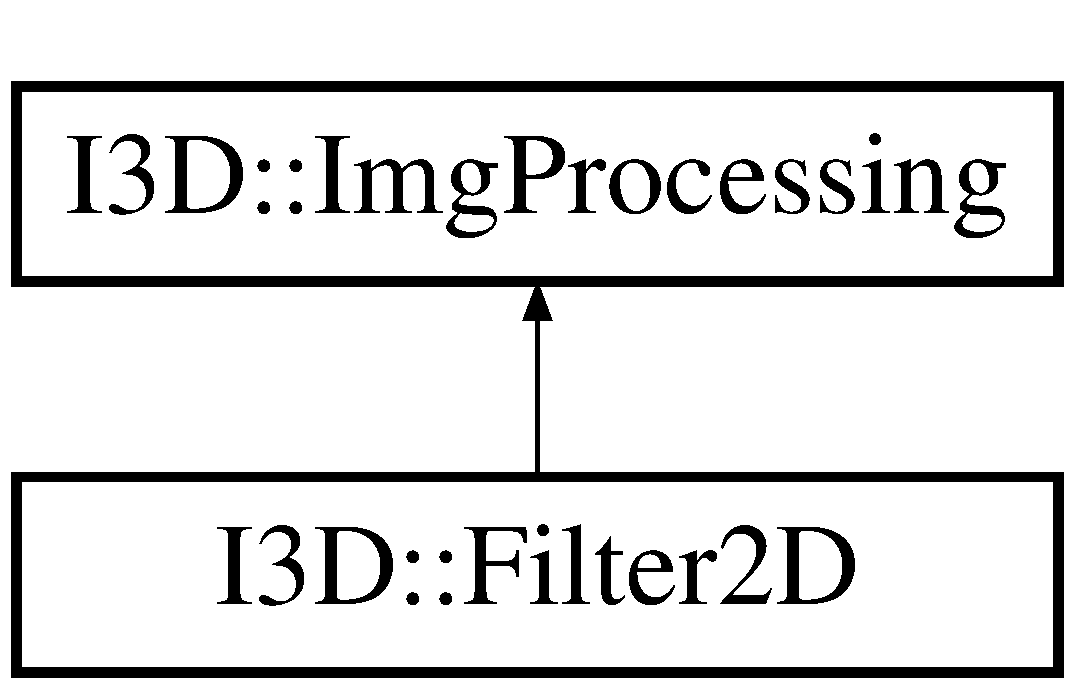
\includegraphics[height=2.000000cm]{class_i3_d_1_1_filter2_d}
\end{center}
\end{figure}
\subsection*{Métodos públicos}
\begin{DoxyCompactItemize}
\item 
\hyperlink{class_i3_d_1_1_filter2_d_aa34212c2a0de19d4eeba64ec222e8a69}{Filter2D} (int ddepth, cv\+::\+Mat kernel, cv\+::\+Point anchor=cv\+::\+Point(-\/1,-\/1), double delta=0, int border\+Type=cv\+::\+B\+O\+R\+D\+E\+R\+\_\+\+C\+O\+N\+S\+T\+A\+NT)
\begin{DoxyCompactList}\small\item\em Constructora clase \hyperlink{class_i3_d_1_1_filter2_d}{Filter2D}. \end{DoxyCompactList}\item 
int \hyperlink{class_i3_d_1_1_filter2_d_a46f44465658be004e62d7e72cc40cb84}{execute} (const cv\+::\+Mat \&mat\+In, cv\+::\+Mat $\ast$mat\+Out) const  override
\begin{DoxyCompactList}\small\item\em Ejecuta el proceso. \end{DoxyCompactList}\item 
void \hyperlink{class_i3_d_1_1_filter2_d_acf15b9a9958739c909768325fad1a3d7}{set\+Parameters} (int ddepth, cv\+::\+Mat kernel, cv\+::\+Point anchor=cv\+::\+Point(-\/1,-\/1), double delta=0, int border\+Type=cv\+::\+B\+O\+R\+D\+E\+R\+\_\+\+C\+O\+N\+S\+T\+A\+NT)
\begin{DoxyCompactList}\small\item\em Establece los parámetros del filtro de convolución. \end{DoxyCompactList}\end{DoxyCompactItemize}
\subsection*{Otros miembros heredados}


\subsection{Descripción detallada}
Aplica un filtrado mediante una matriz de convolución. 

\subsection{Documentación del constructor y destructor}
\index{I3\+D\+::\+Filter2D@{I3\+D\+::\+Filter2D}!Filter2D@{Filter2D}}
\index{Filter2D@{Filter2D}!I3\+D\+::\+Filter2D@{I3\+D\+::\+Filter2D}}
\subsubsection[{\texorpdfstring{Filter2\+D(int ddepth, cv\+::\+Mat kernel, cv\+::\+Point anchor=cv\+::\+Point(-\/1,-\/1), double delta=0, int border\+Type=cv\+::\+B\+O\+R\+D\+E\+R\+\_\+\+C\+O\+N\+S\+T\+A\+N\+T)}{Filter2D(int ddepth, cv::Mat kernel, cv::Point anchor=cv::Point(-1,-1), double delta=0, int borderType=cv::BORDER_CONSTANT)}}]{\setlength{\rightskip}{0pt plus 5cm}I3\+D\+::\+Filter2\+D\+::\+Filter2D (
\begin{DoxyParamCaption}
\item[{int}]{ddepth, }
\item[{cv\+::\+Mat}]{kernel, }
\item[{cv\+::\+Point}]{anchor = {\ttfamily cv\+:\+:Point(-\/1,~-\/1)}, }
\item[{double}]{delta = {\ttfamily 0}, }
\item[{int}]{border\+Type = {\ttfamily cv\+:\+:BORDER\+\_\+CONSTANT}}
\end{DoxyParamCaption}
)\hspace{0.3cm}{\ttfamily [inline]}}\hypertarget{class_i3_d_1_1_filter2_d_aa34212c2a0de19d4eeba64ec222e8a69}{}\label{class_i3_d_1_1_filter2_d_aa34212c2a0de19d4eeba64ec222e8a69}


Constructora clase \hyperlink{class_i3_d_1_1_filter2_d}{Filter2D}. 


\begin{DoxyParams}[1]{Parámetros}
\mbox{\tt in}  & {\em ddepth} & Profundidad de la imagen de destino. ddepth=-\/1\+: Misma profundidad que la imagen de origen \\
\hline
\mbox{\tt in}  & {\em kernel} & Matriz de convolución \\
\hline
\mbox{\tt in}  & {\em anchor} & Punto de anclaje. Por defecto es el centro del kernel \\
\hline
\mbox{\tt in}  & {\em delta} & Valor opcional añadido a los píxeles filtrados \\
\hline
\mbox{\tt in}  & {\em border\+Type} & Método de extrapolación \\
\hline
\end{DoxyParams}


\subsection{Documentación de las funciones miembro}
\index{I3\+D\+::\+Filter2D@{I3\+D\+::\+Filter2D}!execute@{execute}}
\index{execute@{execute}!I3\+D\+::\+Filter2D@{I3\+D\+::\+Filter2D}}
\subsubsection[{\texorpdfstring{execute(const cv\+::\+Mat \&mat\+In, cv\+::\+Mat $\ast$mat\+Out) const  override}{execute(const cv::Mat &matIn, cv::Mat *matOut) const  override}}]{\setlength{\rightskip}{0pt plus 5cm}int I3\+D\+::\+Filter2\+D\+::execute (
\begin{DoxyParamCaption}
\item[{const cv\+::\+Mat \&}]{mat\+In, }
\item[{cv\+::\+Mat $\ast$}]{mat\+Out}
\end{DoxyParamCaption}
) const\hspace{0.3cm}{\ttfamily [override]}, {\ttfamily [virtual]}}\hypertarget{class_i3_d_1_1_filter2_d_a46f44465658be004e62d7e72cc40cb84}{}\label{class_i3_d_1_1_filter2_d_a46f44465658be004e62d7e72cc40cb84}


Ejecuta el proceso. 


\begin{DoxyParams}[1]{Parámetros}
\mbox{\tt in}  & {\em mat\+In} & Imagen de entrada \\
\hline
\mbox{\tt out}  & {\em mat\+Out} & Imagen de salida \\
\hline
\end{DoxyParams}
\begin{DoxyReturn}{Devuelve}
Error. Si los procesos se ejecutan correctamente devuelve 0. 
\end{DoxyReturn}


Implementa \hyperlink{class_i3_d_1_1_img_processing_a74195f05bbf034566e9ff6e10f3af4c9}{I3\+D\+::\+Img\+Processing}.

\index{I3\+D\+::\+Filter2D@{I3\+D\+::\+Filter2D}!set\+Parameters@{set\+Parameters}}
\index{set\+Parameters@{set\+Parameters}!I3\+D\+::\+Filter2D@{I3\+D\+::\+Filter2D}}
\subsubsection[{\texorpdfstring{set\+Parameters(int ddepth, cv\+::\+Mat kernel, cv\+::\+Point anchor=cv\+::\+Point(-\/1,-\/1), double delta=0, int border\+Type=cv\+::\+B\+O\+R\+D\+E\+R\+\_\+\+C\+O\+N\+S\+T\+A\+N\+T)}{setParameters(int ddepth, cv::Mat kernel, cv::Point anchor=cv::Point(-1,-1), double delta=0, int borderType=cv::BORDER_CONSTANT)}}]{\setlength{\rightskip}{0pt plus 5cm}void I3\+D\+::\+Filter2\+D\+::set\+Parameters (
\begin{DoxyParamCaption}
\item[{int}]{ddepth, }
\item[{cv\+::\+Mat}]{kernel, }
\item[{cv\+::\+Point}]{anchor = {\ttfamily cv\+:\+:Point(-\/1,~-\/1)}, }
\item[{double}]{delta = {\ttfamily 0}, }
\item[{int}]{border\+Type = {\ttfamily cv\+:\+:BORDER\+\_\+CONSTANT}}
\end{DoxyParamCaption}
)}\hypertarget{class_i3_d_1_1_filter2_d_acf15b9a9958739c909768325fad1a3d7}{}\label{class_i3_d_1_1_filter2_d_acf15b9a9958739c909768325fad1a3d7}


Establece los parámetros del filtro de convolución. 


\begin{DoxyParams}[1]{Parámetros}
\mbox{\tt in}  & {\em ddepth} & Profundidad de la imagen de destino. ddepth=-\/1\+: Misma profundidad que la imagen de origen \\
\hline
\mbox{\tt in}  & {\em kernel} & Matriz de convolución \\
\hline
\mbox{\tt in}  & {\em anchor} & Punto de anclaje. Por defecto es el centro del kernel \\
\hline
\mbox{\tt in}  & {\em delta} & Valor opcional añadido a los píxeles filtrados \\
\hline
\mbox{\tt in}  & {\em border\+Type} & Método de extrapolación \\
\hline
\end{DoxyParams}


La documentación para esta clase fue generada a partir de los siguientes ficheros\+:\begin{DoxyCompactItemize}
\item 
C\+:/\+Desarrollo/tidop/src/\hyperlink{_img_processing_8h}{Img\+Processing.\+h}\item 
C\+:/\+Desarrollo/tidop/src/\hyperlink{_img_processing_8cpp}{Img\+Processing.\+cpp}\end{DoxyCompactItemize}

\hypertarget{class_i3_d_1_1_function_process}{}\section{Referencia de la Clase I3D\+:\+:Function\+Process}
\label{class_i3_d_1_1_function_process}\index{I3\+D\+::\+Function\+Process@{I3\+D\+::\+Function\+Process}}


Wrapper de una función para ejecutarla como un proceso.  




{\ttfamily \#include $<$Img\+Processing.\+h$>$}

Diagrama de herencias de I3D\+:\+:Function\+Process\begin{figure}[H]
\begin{center}
\leavevmode
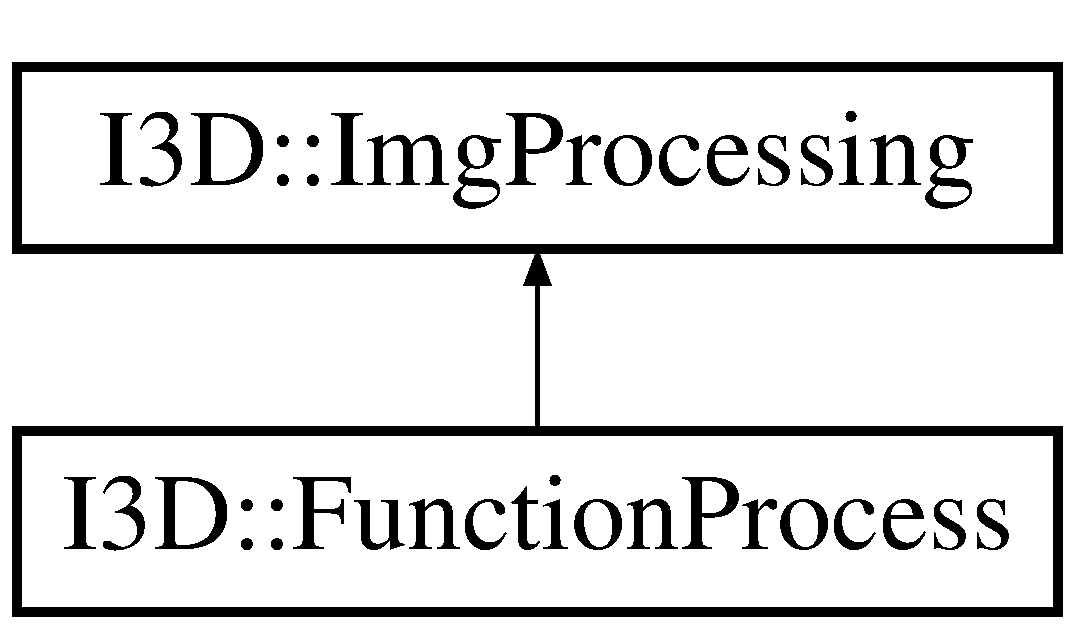
\includegraphics[height=2.000000cm]{class_i3_d_1_1_function_process}
\end{center}
\end{figure}
\subsection*{Métodos públicos}
\begin{DoxyCompactItemize}
\item 
\hyperlink{class_i3_d_1_1_function_process_ae88e4f43dbad5a24dddcbc76811f454f}{Function\+Process} (std\+::function$<$ void(const cv\+::\+Mat \&, cv\+::\+Mat $\ast$)$>$ f)
\begin{DoxyCompactList}\small\item\em Constructora. \end{DoxyCompactList}\item 
int \hyperlink{class_i3_d_1_1_function_process_aa321eb93219271fa3f841538b61133c3}{execute} (const cv\+::\+Mat \&mat\+In, cv\+::\+Mat $\ast$mat\+Out) const  override
\begin{DoxyCompactList}\small\item\em Ejecuta el proceso. \end{DoxyCompactList}\end{DoxyCompactItemize}
\subsection*{Otros miembros heredados}


\subsection{Descripción detallada}
Wrapper de una función para ejecutarla como un proceso. 

Para permitir una mayor libertad en el procesado de las imagenes mediante \hyperlink{class_i3_d_1_1_img_processing_list}{Img\+Processing\+List} se permite asociar una función o lambda a un proceso. La función tiene que ser de la forma\+: \begin{quote}
std\+::function$<$void(const cv\+::\+Mat \&,cv\+::\+Mat $\ast$)$>$ \end{quote}
o si es una lambda\+: \begin{quote}
\mbox{[}\mbox{]}(const cv\+::\+Mat \&in, cv\+::\+Mat $\ast$out) \{ ... \}\end{quote}
\paragraph*{Ejemplo\+:}


\begin{DoxyCode}
std::shared\_ptr<FunctionProcess> fProcess1 = std::make\_shared<FunctionProcess>(
  [](\textcolor{keyword}{const} cv::Mat &in, cv::Mat *out) \{
    in.convertTo(*out, CV\_32F);
\});
std::shared\_ptr<FunctionProcess> fProcess2 = std::make\_shared<FunctionProcess>(
[&](\textcolor{keyword}{const} cv::Mat &in, cv::Mat *out) \{
cv::normalize(in, *out, 0, 255, CV\_MINMAX);
out->convertTo(*out, CV\_8U);
\});

\hyperlink{class_i3_d_1_1_img_processing_list}{I3D::ImgProcessingList} imgprolist\{ fProcess1, fProcess2 \};
\end{DoxyCode}
 

\subsection{Documentación del constructor y destructor}
\index{I3\+D\+::\+Function\+Process@{I3\+D\+::\+Function\+Process}!Function\+Process@{Function\+Process}}
\index{Function\+Process@{Function\+Process}!I3\+D\+::\+Function\+Process@{I3\+D\+::\+Function\+Process}}
\subsubsection[{\texorpdfstring{Function\+Process(std\+::function$<$ void(const cv\+::\+Mat \&, cv\+::\+Mat $\ast$)$>$ f)}{FunctionProcess(std::function< void(const cv::Mat &, cv::Mat *)> f)}}]{\setlength{\rightskip}{0pt plus 5cm}I3\+D\+::\+Function\+Process\+::\+Function\+Process (
\begin{DoxyParamCaption}
\item[{std\+::function$<$ void(const cv\+::\+Mat \&, cv\+::\+Mat $\ast$)$>$}]{f}
\end{DoxyParamCaption}
)\hspace{0.3cm}{\ttfamily [inline]}}\hypertarget{class_i3_d_1_1_function_process_ae88e4f43dbad5a24dddcbc76811f454f}{}\label{class_i3_d_1_1_function_process_ae88e4f43dbad5a24dddcbc76811f454f}


Constructora. 


\begin{DoxyParams}[1]{Parámetros}
\mbox{\tt in}  & {\em f} & Función de la forma std\+::function$<$void(const cv\+::\+Mat \&,cv\+::\+Mat $\ast$)$>$ \\
\hline
\end{DoxyParams}


\subsection{Documentación de las funciones miembro}
\index{I3\+D\+::\+Function\+Process@{I3\+D\+::\+Function\+Process}!execute@{execute}}
\index{execute@{execute}!I3\+D\+::\+Function\+Process@{I3\+D\+::\+Function\+Process}}
\subsubsection[{\texorpdfstring{execute(const cv\+::\+Mat \&mat\+In, cv\+::\+Mat $\ast$mat\+Out) const  override}{execute(const cv::Mat &matIn, cv::Mat *matOut) const  override}}]{\setlength{\rightskip}{0pt plus 5cm}int I3\+D\+::\+Function\+Process\+::execute (
\begin{DoxyParamCaption}
\item[{const cv\+::\+Mat \&}]{mat\+In, }
\item[{cv\+::\+Mat $\ast$}]{mat\+Out}
\end{DoxyParamCaption}
) const\hspace{0.3cm}{\ttfamily [override]}, {\ttfamily [virtual]}}\hypertarget{class_i3_d_1_1_function_process_aa321eb93219271fa3f841538b61133c3}{}\label{class_i3_d_1_1_function_process_aa321eb93219271fa3f841538b61133c3}


Ejecuta el proceso. 


\begin{DoxyParams}[1]{Parámetros}
\mbox{\tt in}  & {\em mat\+In} & Imagen de entrada. \\
\hline
\mbox{\tt out}  & {\em mat\+Out} & Imagen de salida. \\
\hline
\end{DoxyParams}
\begin{DoxyReturn}{Devuelve}
Error. Si los procesos se ejecutan correctamente devuelve 0. 
\end{DoxyReturn}


Implementa \hyperlink{class_i3_d_1_1_img_processing_a74195f05bbf034566e9ff6e10f3af4c9}{I3\+D\+::\+Img\+Processing}.



La documentación para esta clase fue generada a partir de los siguientes ficheros\+:\begin{DoxyCompactItemize}
\item 
C\+:/\+Desarrollo/tidop/src/\hyperlink{_img_processing_8h}{Img\+Processing.\+h}\item 
C\+:/\+Desarrollo/tidop/src/\hyperlink{_img_processing_8cpp}{Img\+Processing.\+cpp}\end{DoxyCompactItemize}

\hypertarget{class_i3_d_1_1_gaussian_blur}{}\section{Referencia de la Clase I3D\+:\+:Gaussian\+Blur}
\label{class_i3_d_1_1_gaussian_blur}\index{I3\+D\+::\+Gaussian\+Blur@{I3\+D\+::\+Gaussian\+Blur}}


Desenfoque gaussiano.  




{\ttfamily \#include $<$Img\+Processing.\+h$>$}

Diagrama de herencias de I3D\+:\+:Gaussian\+Blur\begin{figure}[H]
\begin{center}
\leavevmode
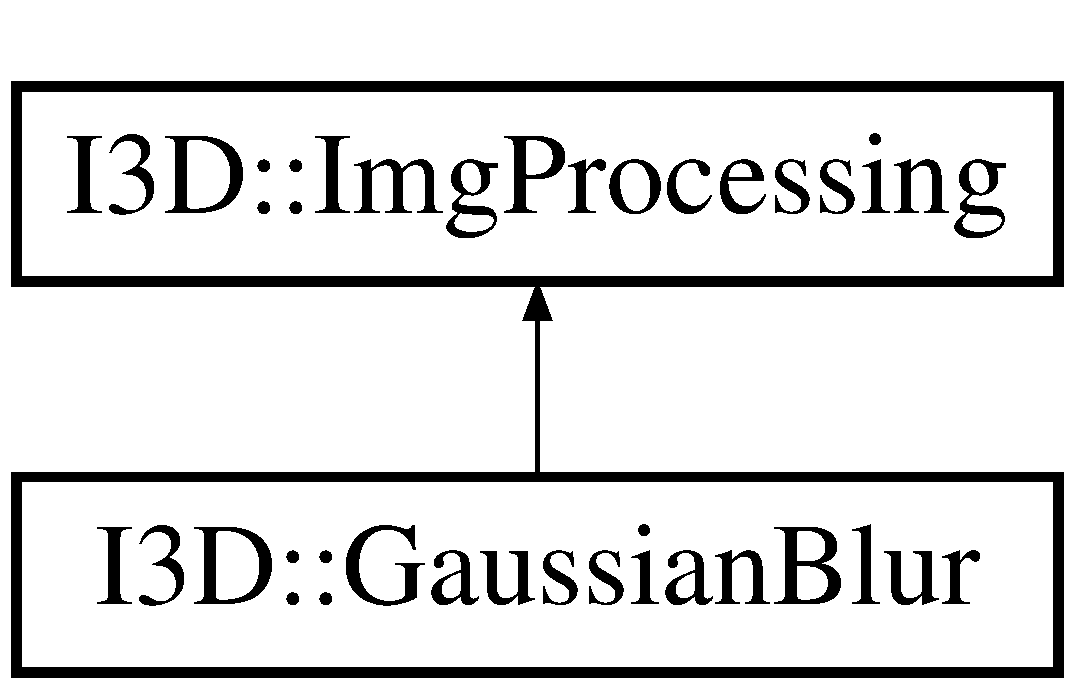
\includegraphics[height=2.000000cm]{class_i3_d_1_1_gaussian_blur}
\end{center}
\end{figure}
\subsection*{Métodos públicos}
\begin{DoxyCompactItemize}
\item 
\hyperlink{class_i3_d_1_1_gaussian_blur_ae83c05d57cb336bff56230338c33da38}{Gaussian\+Blur} (cv\+::\+Size size, double sigmaX, double sigmaY=0., int border\+Type=4)
\begin{DoxyCompactList}\small\item\em \hyperlink{class_i3_d_1_1_gaussian_blur}{Gaussian\+Blur}. \end{DoxyCompactList}\item 
int \hyperlink{class_i3_d_1_1_gaussian_blur_a19812cea51167dd35e8a85d3178061d5}{execute} (const cv\+::\+Mat \&mat\+In, cv\+::\+Mat $\ast$mat\+Out) const  override
\begin{DoxyCompactList}\small\item\em Ejecuta el proceso. \end{DoxyCompactList}\item 
void \hyperlink{class_i3_d_1_1_gaussian_blur_a8d22c6f666e7939aaeaecf3a752f464a}{set\+Parameters} (cv\+::\+Size k\+Size, double sigmaX, double sigmaY=0, int border\+Type=4)
\begin{DoxyCompactList}\small\item\em Establece los parámetros. \end{DoxyCompactList}\end{DoxyCompactItemize}
\subsection*{Otros miembros heredados}


\subsection{Descripción detallada}
Desenfoque gaussiano. 

\subsection{Documentación del constructor y destructor}
\index{I3\+D\+::\+Gaussian\+Blur@{I3\+D\+::\+Gaussian\+Blur}!Gaussian\+Blur@{Gaussian\+Blur}}
\index{Gaussian\+Blur@{Gaussian\+Blur}!I3\+D\+::\+Gaussian\+Blur@{I3\+D\+::\+Gaussian\+Blur}}
\subsubsection[{\texorpdfstring{Gaussian\+Blur(cv\+::\+Size size, double sigma\+X, double sigma\+Y=0., int border\+Type=4)}{GaussianBlur(cv::Size size, double sigmaX, double sigmaY=0., int borderType=4)}}]{\setlength{\rightskip}{0pt plus 5cm}I3\+D\+::\+Gaussian\+Blur\+::\+Gaussian\+Blur (
\begin{DoxyParamCaption}
\item[{cv\+::\+Size}]{size, }
\item[{double}]{sigmaX, }
\item[{double}]{sigmaY = {\ttfamily 0.}, }
\item[{int}]{border\+Type = {\ttfamily 4}}
\end{DoxyParamCaption}
)\hspace{0.3cm}{\ttfamily [inline]}}\hypertarget{class_i3_d_1_1_gaussian_blur_ae83c05d57cb336bff56230338c33da38}{}\label{class_i3_d_1_1_gaussian_blur_ae83c05d57cb336bff56230338c33da38}


\hyperlink{class_i3_d_1_1_gaussian_blur}{Gaussian\+Blur}. 


\begin{DoxyParams}[1]{Parámetros}
\mbox{\tt in}  & {\em size} & Tamaño del kernel \\
\hline
\mbox{\tt in}  & {\em sigmaX} & Desviación estándar del kernel en la dirección X. \\
\hline
\mbox{\tt in}  & {\em sigmaY} & Desviación estándar del kernel en la dirección Y. \\
\hline
\mbox{\tt in}  & {\em border\+Type} & Método de extrapolación (cv\+::\+Border\+Types) \\
\hline
\end{DoxyParams}


\subsection{Documentación de las funciones miembro}
\index{I3\+D\+::\+Gaussian\+Blur@{I3\+D\+::\+Gaussian\+Blur}!execute@{execute}}
\index{execute@{execute}!I3\+D\+::\+Gaussian\+Blur@{I3\+D\+::\+Gaussian\+Blur}}
\subsubsection[{\texorpdfstring{execute(const cv\+::\+Mat \&mat\+In, cv\+::\+Mat $\ast$mat\+Out) const  override}{execute(const cv::Mat &matIn, cv::Mat *matOut) const  override}}]{\setlength{\rightskip}{0pt plus 5cm}int I3\+D\+::\+Gaussian\+Blur\+::execute (
\begin{DoxyParamCaption}
\item[{const cv\+::\+Mat \&}]{mat\+In, }
\item[{cv\+::\+Mat $\ast$}]{mat\+Out}
\end{DoxyParamCaption}
) const\hspace{0.3cm}{\ttfamily [override]}, {\ttfamily [virtual]}}\hypertarget{class_i3_d_1_1_gaussian_blur_a19812cea51167dd35e8a85d3178061d5}{}\label{class_i3_d_1_1_gaussian_blur_a19812cea51167dd35e8a85d3178061d5}


Ejecuta el proceso. 


\begin{DoxyParams}[1]{Parámetros}
\mbox{\tt in}  & {\em mat\+In} & Imagen de entrada \\
\hline
\mbox{\tt out}  & {\em mat\+Out} & Imagen de salida \\
\hline
\end{DoxyParams}
\begin{DoxyReturn}{Devuelve}
Error. Si los procesos se ejecutan correctamente devuelve 0. 
\end{DoxyReturn}


Implementa \hyperlink{class_i3_d_1_1_img_processing_a74195f05bbf034566e9ff6e10f3af4c9}{I3\+D\+::\+Img\+Processing}.

\index{I3\+D\+::\+Gaussian\+Blur@{I3\+D\+::\+Gaussian\+Blur}!set\+Parameters@{set\+Parameters}}
\index{set\+Parameters@{set\+Parameters}!I3\+D\+::\+Gaussian\+Blur@{I3\+D\+::\+Gaussian\+Blur}}
\subsubsection[{\texorpdfstring{set\+Parameters(cv\+::\+Size k\+Size, double sigma\+X, double sigma\+Y=0, int border\+Type=4)}{setParameters(cv::Size kSize, double sigmaX, double sigmaY=0, int borderType=4)}}]{\setlength{\rightskip}{0pt plus 5cm}void I3\+D\+::\+Gaussian\+Blur\+::set\+Parameters (
\begin{DoxyParamCaption}
\item[{cv\+::\+Size}]{k\+Size, }
\item[{double}]{sigmaX, }
\item[{double}]{sigmaY = {\ttfamily 0}, }
\item[{int}]{border\+Type = {\ttfamily 4}}
\end{DoxyParamCaption}
)}\hypertarget{class_i3_d_1_1_gaussian_blur_a8d22c6f666e7939aaeaecf3a752f464a}{}\label{class_i3_d_1_1_gaussian_blur_a8d22c6f666e7939aaeaecf3a752f464a}


Establece los parámetros. 


\begin{DoxyParams}[1]{Parámetros}
\mbox{\tt in}  & {\em k\+Size} & Tamaño del kernel \\
\hline
\mbox{\tt in}  & {\em sigmaX} & Desviación estándar del kernel en la dirección X \\
\hline
\mbox{\tt in}  & {\em sigmaY} & Desviación estándar del kernel en la dirección Y \\
\hline
\mbox{\tt in}  & {\em border\+Type} & Método de extrapolación (cv\+::\+Border\+Types) \\
\hline
\end{DoxyParams}


La documentación para esta clase fue generada a partir de los siguientes ficheros\+:\begin{DoxyCompactItemize}
\item 
D\+:/\+Desarrollo/tidop/src/\hyperlink{_img_processing_8h}{Img\+Processing.\+h}\item 
D\+:/\+Desarrollo/tidop/src/\hyperlink{_img_processing_8cpp}{Img\+Processing.\+cpp}\end{DoxyCompactItemize}

\hypertarget{class_i3_d_1_1_gradient}{}\section{Referencia de la Clase I3D\+:\+:Gradient}
\label{class_i3_d_1_1_gradient}\index{I3\+D\+::\+Gradient@{I3\+D\+::\+Gradient}}


Operación morfológica gradiente \hyperlink{class_i3_d_1_1_gradient}{Gradient} = dilation -\/ erosion.  




{\ttfamily \#include $<$Img\+Processing.\+h$>$}

Diagrama de herencias de I3D\+:\+:Gradient\begin{figure}[H]
\begin{center}
\leavevmode
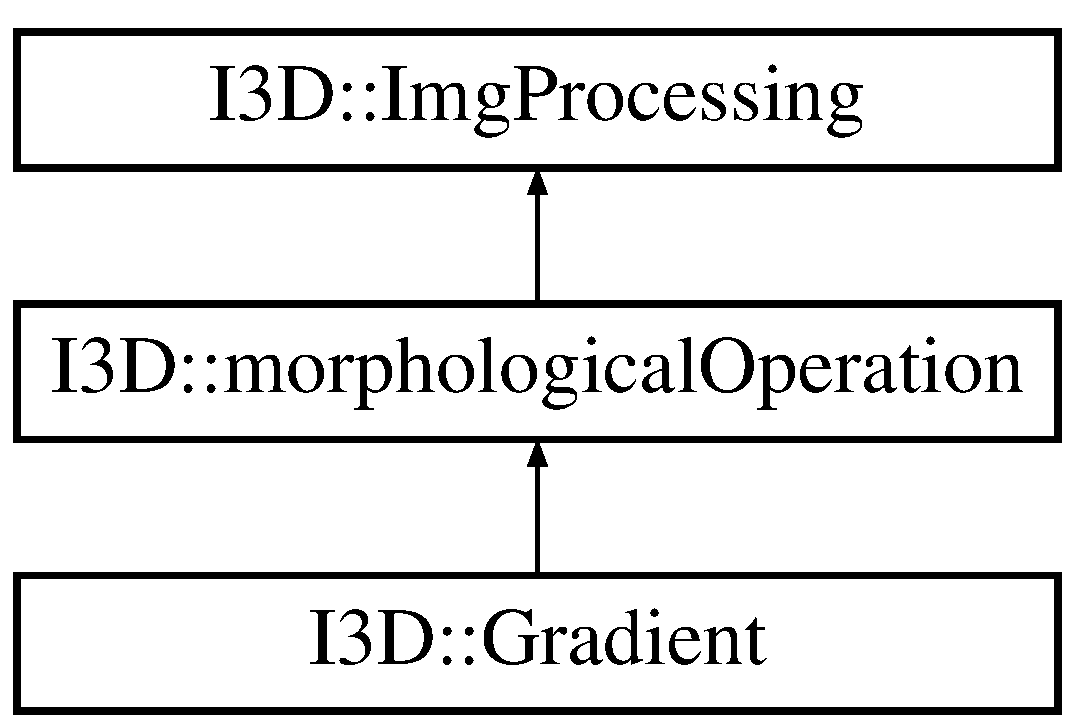
\includegraphics[height=3.000000cm]{class_i3_d_1_1_gradient}
\end{center}
\end{figure}
\subsection*{Métodos públicos}
\begin{DoxyCompactItemize}
\item 
\hyperlink{class_i3_d_1_1_gradient_a42a6683ae715e8c86dfd9bee662f01e5}{Gradient} (int size, cv\+::\+Morph\+Shapes shapes=cv\+::\+M\+O\+R\+P\+H\+\_\+\+R\+E\+CT, cv\+::\+Point anchor=cv\+::\+Point(-\/1,-\/1), int iterations=1, int border\+Type=cv\+::\+B\+O\+R\+D\+E\+R\+\_\+\+C\+O\+N\+S\+T\+A\+NT, const cv\+::\+Scalar \&border\+Value=cv\+::morphology\+Default\+Border\+Value())
\begin{DoxyCompactList}\small\item\em Constructora clase \hyperlink{class_i3_d_1_1_closing}{Closing}. \end{DoxyCompactList}\end{DoxyCompactItemize}
\subsection*{Otros miembros heredados}


\subsection{Descripción detallada}
Operación morfológica gradiente \hyperlink{class_i3_d_1_1_gradient}{Gradient} = dilation -\/ erosion. 

\subsection{Documentación del constructor y destructor}
\index{I3\+D\+::\+Gradient@{I3\+D\+::\+Gradient}!Gradient@{Gradient}}
\index{Gradient@{Gradient}!I3\+D\+::\+Gradient@{I3\+D\+::\+Gradient}}
\subsubsection[{\texorpdfstring{Gradient(int size, cv\+::\+Morph\+Shapes shapes=cv\+::\+M\+O\+R\+P\+H\+\_\+\+R\+E\+C\+T, cv\+::\+Point anchor=cv\+::\+Point(-\/1,-\/1), int iterations=1, int border\+Type=cv\+::\+B\+O\+R\+D\+E\+R\+\_\+\+C\+O\+N\+S\+T\+A\+N\+T, const cv\+::\+Scalar \&border\+Value=cv\+::morphology\+Default\+Border\+Value())}{Gradient(int size, cv::MorphShapes shapes=cv::MORPH_RECT, cv::Point anchor=cv::Point(-1,-1), int iterations=1, int borderType=cv::BORDER_CONSTANT, const cv::Scalar &borderValue=cv::morphologyDefaultBorderValue())}}]{\setlength{\rightskip}{0pt plus 5cm}I3\+D\+::\+Gradient\+::\+Gradient (
\begin{DoxyParamCaption}
\item[{int}]{size, }
\item[{cv\+::\+Morph\+Shapes}]{shapes = {\ttfamily cv\+:\+:MORPH\+\_\+RECT}, }
\item[{cv\+::\+Point}]{anchor = {\ttfamily cv\+:\+:Point(-\/1,~-\/1)}, }
\item[{int}]{iterations = {\ttfamily 1}, }
\item[{int}]{border\+Type = {\ttfamily cv\+:\+:BORDER\+\_\+CONSTANT}, }
\item[{const cv\+::\+Scalar \&}]{border\+Value = {\ttfamily cv\+:\+:morphologyDefaultBorderValue()}}
\end{DoxyParamCaption}
)\hspace{0.3cm}{\ttfamily [inline]}}\hypertarget{class_i3_d_1_1_gradient_a42a6683ae715e8c86dfd9bee662f01e5}{}\label{class_i3_d_1_1_gradient_a42a6683ae715e8c86dfd9bee662f01e5}


Constructora clase \hyperlink{class_i3_d_1_1_closing}{Closing}. 


\begin{DoxyParams}[1]{Parámetros}
\mbox{\tt in}  & {\em size} & \\
\hline
\mbox{\tt in}  & {\em type} & \\
\hline
\mbox{\tt in}  & {\em anchor} & Punto de anclaje. Por defecto es el centro del kernel \\
\hline
\mbox{\tt in}  & {\em iterations} & \\
\hline
\mbox{\tt in}  & {\em border\+Type} & Método de extrapolación \\
\hline
\mbox{\tt in}  & {\em border\+Value} & \\
\hline
\end{DoxyParams}


La documentación para esta clase fue generada a partir del siguiente fichero\+:\begin{DoxyCompactItemize}
\item 
C\+:/\+Desarrollo/tidop/src/\hyperlink{_img_processing_8h}{Img\+Processing.\+h}\end{DoxyCompactItemize}

\hypertarget{class_i3_d_1_1_helmert2_d}{}\section{Referencia de la plantilla de la Clase I3D\+:\+:Helmert2D$<$ T $>$}
\label{class_i3_d_1_1_helmert2_d}\index{I3\+D\+::\+Helmert2\+D$<$ T $>$@{I3\+D\+::\+Helmert2\+D$<$ T $>$}}


Helmert 2D.  




{\ttfamily \#include $<$transform.\+h$>$}

Diagrama de herencias de I3D\+:\+:Helmert2D$<$ T $>$\begin{figure}[H]
\begin{center}
\leavevmode
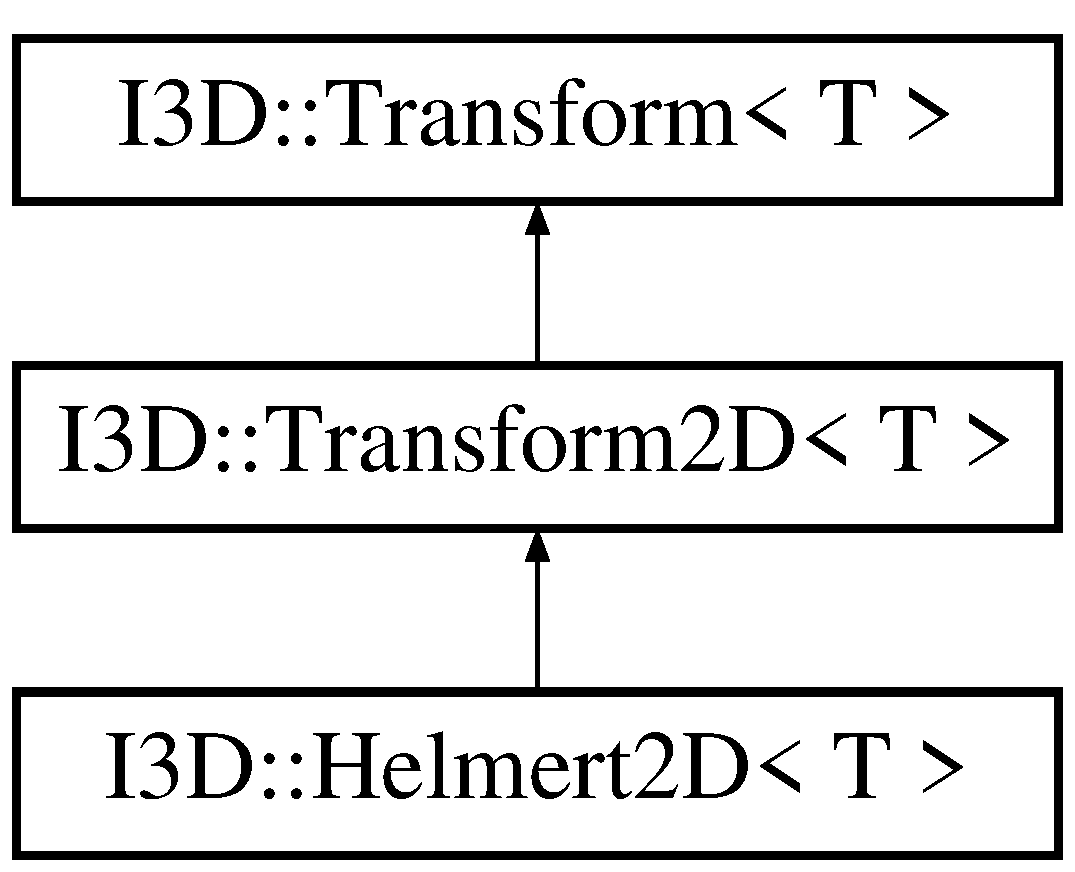
\includegraphics[height=3.000000cm]{class_i3_d_1_1_helmert2_d}
\end{center}
\end{figure}
\subsection*{Métodos públicos}
\begin{DoxyCompactItemize}
\item 
\hyperlink{class_i3_d_1_1_helmert2_d_a8eca7720410824fb11469d8d893fb2d6}{Helmert2D} ()
\begin{DoxyCompactList}\small\item\em Constructor por defecto. \end{DoxyCompactList}\item 
\hyperlink{class_i3_d_1_1_helmert2_d_a810553f036b0e7ecf77e31246dc8edea}{Helmert2D} (\hyperlink{class_i3_d_1_1_transform_ac087b4b8b9acb1b11a6caa2231d598c7}{sub\+\_\+type} \hyperlink{class_i3_d_1_1_helmert2_d_ad0bb6ad335ff383cf85f29a3da60c2e7}{x0}, \hyperlink{class_i3_d_1_1_transform_ac087b4b8b9acb1b11a6caa2231d598c7}{sub\+\_\+type} \hyperlink{class_i3_d_1_1_helmert2_d_a60ddf8a70434410bc53e610abf583dbe}{y0}, double scale, double rotation)
\begin{DoxyCompactList}\small\item\em Constructor. \end{DoxyCompactList}\item 
bool \hyperlink{group__trf2_d_group_ga300279dee0a002835c25322bd2ea9398}{compute} (const std\+::vector$<$ T $>$ \&pts1, const std\+::vector$<$ T $>$ \&pts2) override
\begin{DoxyCompactList}\small\item\em Calcula la transformación Helmert 2D entre dos sistemas diferentes a partir de dos conjuntos de puntos en cada sistema. \end{DoxyCompactList}\item 
void \hyperlink{group__trf2_d_group_gab7354b67b291bf01b3fd045578598fb1}{transform} (const std\+::vector$<$ T $>$ \&in, std\+::vector$<$ T $>$ $\ast$out, bool b\+Direct=true) const  override
\begin{DoxyCompactList}\small\item\em Transforma un conjunto de puntos en otro aplicando un helmert 2D. \end{DoxyCompactList}\item 
void \hyperlink{group__trf2_d_group_ga11e1634259f4e3085840a16c3bfb314e}{transform} (const T \&in, T $\ast$out, bool b\+Direct=true) const 
\begin{DoxyCompactList}\small\item\em Aplica un helmert 2D a un punto. \end{DoxyCompactList}\item 
T \hyperlink{group__trf2_d_group_gaa9495c4b5fe0dbfb703a2004b41e310b}{transform} (const T \&in, bool b\+Direct=true) const 
\begin{DoxyCompactList}\small\item\em Aplica un helmert 2D a un punto. \end{DoxyCompactList}\item 
double \hyperlink{class_i3_d_1_1_helmert2_d_a7f96184b77dfd19734906e8ea79ec74f}{get\+Rotation} () const 
\begin{DoxyCompactList}\small\item\em Devuelve el giro. \end{DoxyCompactList}\item 
double \hyperlink{class_i3_d_1_1_helmert2_d_ad748a42c6267e30b8dc009714cc07559}{get\+Scale} () const 
\begin{DoxyCompactList}\small\item\em Devuelve la escala de la transformación. \end{DoxyCompactList}\item 
void \hyperlink{group__trf2_d_group_ga792554ed5f33a824b0c619e156697022}{set\+Parameters} (T \hyperlink{class_i3_d_1_1_helmert2_d_ad0bb6ad335ff383cf85f29a3da60c2e7}{x0}, T \hyperlink{class_i3_d_1_1_helmert2_d_a60ddf8a70434410bc53e610abf583dbe}{y0}, double scale, double rotation)
\begin{DoxyCompactList}\small\item\em Establece los parámetros. \end{DoxyCompactList}\item 
void \hyperlink{group__trf2_d_group_gaf7d2a6c0aeeb81c66b8e07e55236a6d2}{set\+Rotation} (double rotation)
\begin{DoxyCompactList}\small\item\em Establece la rotación de la transformación. \end{DoxyCompactList}\item 
void \hyperlink{group__trf2_d_group_gaa732c2f1d68f41b1ab4ca63aa40b21df}{set\+Scale} (double scale)
\begin{DoxyCompactList}\small\item\em Establece la escala de la transformación. \end{DoxyCompactList}\end{DoxyCompactItemize}
\subsection*{Atributos públicos}
\begin{DoxyCompactItemize}
\item 
\hyperlink{class_i3_d_1_1_transform_ac087b4b8b9acb1b11a6caa2231d598c7}{sub\+\_\+type} \hyperlink{class_i3_d_1_1_helmert2_d_ad0bb6ad335ff383cf85f29a3da60c2e7}{x0}
\begin{DoxyCompactList}\small\item\em Traslación en x. \end{DoxyCompactList}\item 
\hyperlink{class_i3_d_1_1_transform_ac087b4b8b9acb1b11a6caa2231d598c7}{sub\+\_\+type} \hyperlink{class_i3_d_1_1_helmert2_d_a60ddf8a70434410bc53e610abf583dbe}{y0}
\begin{DoxyCompactList}\small\item\em Traslación en y. \end{DoxyCompactList}\end{DoxyCompactItemize}
\subsection*{Otros miembros heredados}


\subsection{Descripción detallada}
\subsubsection*{template$<$typename T$>$\\*
class I3\+D\+::\+Helmert2\+D$<$ T $>$}

Helmert 2D. 

El Helmert o Transformación de Semejanza expresa la relación que existe (o transformación que es preciso realizar) entre dos sistemas cartesianos que discrepan en la situación del origen, en la orientación de los ejes y en la unidad de medida a lo largo de los mismos pero de manera que dicha variación en unidad de medida es constante a lo largo de cada eje y entre los dos ejes

\begin{quote}
a = scale $\ast$ cos(rotation); ~\newline
 b = scale $\ast$ sin(rotation);

x\textquotesingle{} = a $\ast$ x + b $\ast$ y + X0 ~\newline
 y\textquotesingle{} = a $\ast$ x -\/ b $\ast$ x + Y0 \end{quote}


\subsection{Documentación del constructor y destructor}
\index{I3\+D\+::\+Helmert2D@{I3\+D\+::\+Helmert2D}!Helmert2D@{Helmert2D}}
\index{Helmert2D@{Helmert2D}!I3\+D\+::\+Helmert2D@{I3\+D\+::\+Helmert2D}}
\subsubsection[{\texorpdfstring{Helmert2\+D()}{Helmert2D()}}]{\setlength{\rightskip}{0pt plus 5cm}template$<$typename T $>$ {\bf I3\+D\+::\+Helmert2D}$<$ T $>$\+::{\bf Helmert2D} (
\begin{DoxyParamCaption}
{}
\end{DoxyParamCaption}
)\hspace{0.3cm}{\ttfamily [inline]}}\hypertarget{class_i3_d_1_1_helmert2_d_a8eca7720410824fb11469d8d893fb2d6}{}\label{class_i3_d_1_1_helmert2_d_a8eca7720410824fb11469d8d893fb2d6}


Constructor por defecto. 

\index{I3\+D\+::\+Helmert2D@{I3\+D\+::\+Helmert2D}!Helmert2D@{Helmert2D}}
\index{Helmert2D@{Helmert2D}!I3\+D\+::\+Helmert2D@{I3\+D\+::\+Helmert2D}}
\subsubsection[{\texorpdfstring{Helmert2\+D(sub\+\_\+type x0, sub\+\_\+type y0, double scale, double rotation)}{Helmert2D(sub_type x0, sub_type y0, double scale, double rotation)}}]{\setlength{\rightskip}{0pt plus 5cm}template$<$typename T $>$ {\bf I3\+D\+::\+Helmert2D}$<$ T $>$\+::{\bf Helmert2D} (
\begin{DoxyParamCaption}
\item[{{\bf sub\+\_\+type}}]{x0, }
\item[{{\bf sub\+\_\+type}}]{y0, }
\item[{double}]{scale, }
\item[{double}]{rotation}
\end{DoxyParamCaption}
)\hspace{0.3cm}{\ttfamily [inline]}}\hypertarget{class_i3_d_1_1_helmert2_d_a810553f036b0e7ecf77e31246dc8edea}{}\label{class_i3_d_1_1_helmert2_d_a810553f036b0e7ecf77e31246dc8edea}


Constructor. 


\begin{DoxyParams}[1]{Parámetros}
\mbox{\tt in}  & {\em x0} & Traslación en x \\
\hline
\mbox{\tt in}  & {\em y0} & Traslación en y \\
\hline
\mbox{\tt in}  & {\em scale} & Escala \\
\hline
\mbox{\tt in}  & {\em rotation} & Rotación \\
\hline
\end{DoxyParams}


\subsection{Documentación de las funciones miembro}
\index{I3\+D\+::\+Helmert2D@{I3\+D\+::\+Helmert2D}!get\+Rotation@{get\+Rotation}}
\index{get\+Rotation@{get\+Rotation}!I3\+D\+::\+Helmert2D@{I3\+D\+::\+Helmert2D}}
\subsubsection[{\texorpdfstring{get\+Rotation() const }{getRotation() const }}]{\setlength{\rightskip}{0pt plus 5cm}template$<$typename T $>$ double {\bf I3\+D\+::\+Helmert2D}$<$ T $>$\+::get\+Rotation (
\begin{DoxyParamCaption}
{}
\end{DoxyParamCaption}
) const\hspace{0.3cm}{\ttfamily [inline]}}\hypertarget{class_i3_d_1_1_helmert2_d_a7f96184b77dfd19734906e8ea79ec74f}{}\label{class_i3_d_1_1_helmert2_d_a7f96184b77dfd19734906e8ea79ec74f}


Devuelve el giro. 

\begin{DoxyReturn}{Devuelve}
\mbox{[}in\mbox{]} Ángulo de rotación en radianes 
\end{DoxyReturn}
\index{I3\+D\+::\+Helmert2D@{I3\+D\+::\+Helmert2D}!get\+Scale@{get\+Scale}}
\index{get\+Scale@{get\+Scale}!I3\+D\+::\+Helmert2D@{I3\+D\+::\+Helmert2D}}
\subsubsection[{\texorpdfstring{get\+Scale() const }{getScale() const }}]{\setlength{\rightskip}{0pt plus 5cm}template$<$typename T $>$ double {\bf I3\+D\+::\+Helmert2D}$<$ T $>$\+::get\+Scale (
\begin{DoxyParamCaption}
{}
\end{DoxyParamCaption}
) const\hspace{0.3cm}{\ttfamily [inline]}}\hypertarget{class_i3_d_1_1_helmert2_d_ad748a42c6267e30b8dc009714cc07559}{}\label{class_i3_d_1_1_helmert2_d_ad748a42c6267e30b8dc009714cc07559}


Devuelve la escala de la transformación. 

\begin{DoxyReturn}{Devuelve}
Escala de la transformación 
\end{DoxyReturn}


\subsection{Documentación de los datos miembro}
\index{I3\+D\+::\+Helmert2D@{I3\+D\+::\+Helmert2D}!x0@{x0}}
\index{x0@{x0}!I3\+D\+::\+Helmert2D@{I3\+D\+::\+Helmert2D}}
\subsubsection[{\texorpdfstring{x0}{x0}}]{\setlength{\rightskip}{0pt plus 5cm}template$<$typename T $>$ {\bf sub\+\_\+type} {\bf I3\+D\+::\+Helmert2D}$<$ T $>$\+::x0}\hypertarget{class_i3_d_1_1_helmert2_d_ad0bb6ad335ff383cf85f29a3da60c2e7}{}\label{class_i3_d_1_1_helmert2_d_ad0bb6ad335ff383cf85f29a3da60c2e7}


Traslación en x. 

\index{I3\+D\+::\+Helmert2D@{I3\+D\+::\+Helmert2D}!y0@{y0}}
\index{y0@{y0}!I3\+D\+::\+Helmert2D@{I3\+D\+::\+Helmert2D}}
\subsubsection[{\texorpdfstring{y0}{y0}}]{\setlength{\rightskip}{0pt plus 5cm}template$<$typename T $>$ {\bf sub\+\_\+type} {\bf I3\+D\+::\+Helmert2D}$<$ T $>$\+::y0}\hypertarget{class_i3_d_1_1_helmert2_d_a60ddf8a70434410bc53e610abf583dbe}{}\label{class_i3_d_1_1_helmert2_d_a60ddf8a70434410bc53e610abf583dbe}


Traslación en y. 



La documentación para esta clase fue generada a partir del siguiente fichero\+:\begin{DoxyCompactItemize}
\item 
D\+:/\+Desarrollo/tidop/src/\hyperlink{transform_8h}{transform.\+h}\end{DoxyCompactItemize}

\hypertarget{class_i3_d_1_1_helmert3_d}{}\section{Referencia de la plantilla de la Clase I3D\+:\+:Helmert3D$<$ T $>$}
\label{class_i3_d_1_1_helmert3_d}\index{I3\+D\+::\+Helmert3\+D$<$ T $>$@{I3\+D\+::\+Helmert3\+D$<$ T $>$}}


Helmert 3D.  




{\ttfamily \#include $<$transform.\+h$>$}

Diagrama de herencias de I3D\+:\+:Helmert3D$<$ T $>$\begin{figure}[H]
\begin{center}
\leavevmode
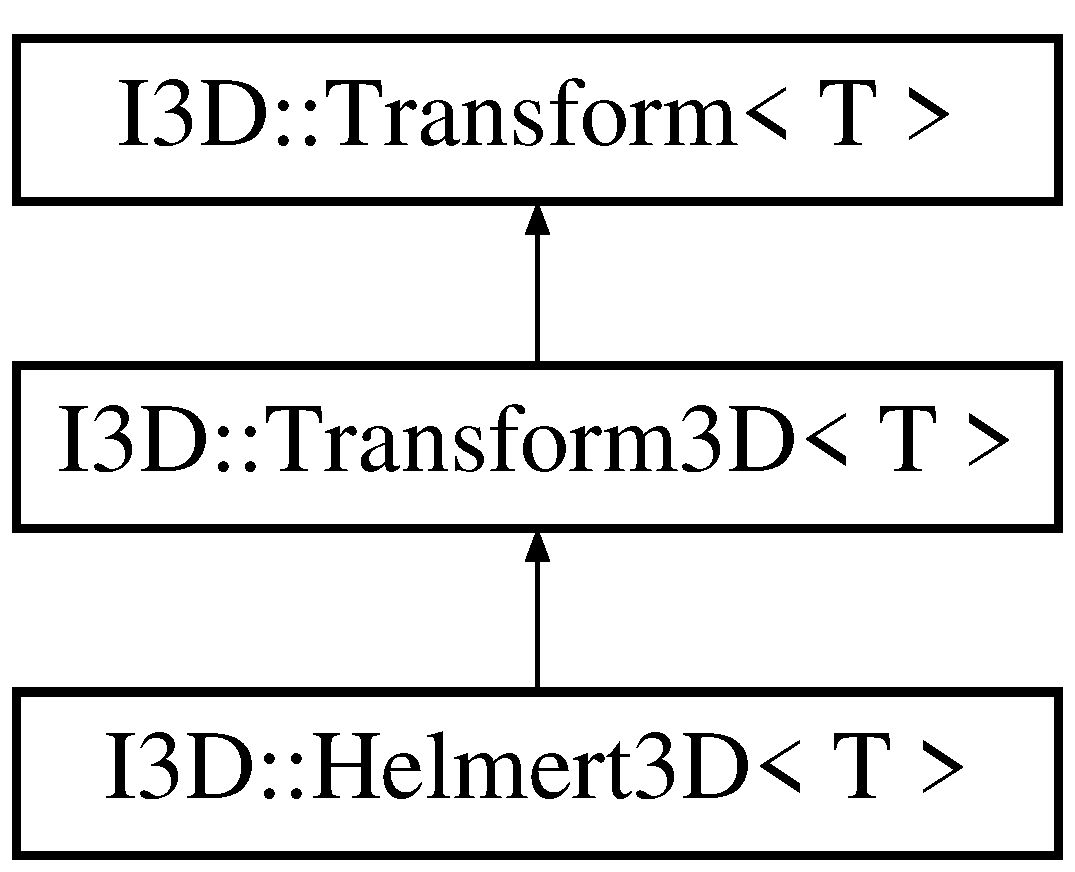
\includegraphics[height=3.000000cm]{class_i3_d_1_1_helmert3_d}
\end{center}
\end{figure}
\subsection*{Métodos públicos}
\begin{DoxyCompactItemize}
\item 
\hyperlink{class_i3_d_1_1_helmert3_d_a3f0ea1eee87fd53c2632ddc78a602f28}{Helmert3D} ()
\begin{DoxyCompactList}\small\item\em Constructor por defecto. \end{DoxyCompactList}\item 
\hyperlink{class_i3_d_1_1_helmert3_d_a4b44e4b5680a999a95f88b05eab127f4}{Helmert3D} (T \hyperlink{class_i3_d_1_1_helmert3_d_a57421e1c701909b5a319dfeaba50fe20}{x0}, T \hyperlink{class_i3_d_1_1_helmert3_d_a8367d52bdb3d60a015e9c30ce7ccacde}{y0}, T \hyperlink{class_i3_d_1_1_helmert3_d_aaa4da06457bac6b987d41a93b9d29d1e}{z0}, double scale, double omega, double phi, double kappa)
\begin{DoxyCompactList}\small\item\em Constructor. \end{DoxyCompactList}\item 
bool \hyperlink{group__trf3_d_group_gaf6c9d07daaca435365b84688326885e3}{compute} (const std\+::vector$<$ T $>$ \&pts1, const std\+::vector$<$ T $>$ \&pts2) override
\begin{DoxyCompactList}\small\item\em Calcula la transformación Helmert 2D entre dos sistemas diferentes a partir de dos conjuntos de puntos en cada sistema. \end{DoxyCompactList}\item 
void \hyperlink{group__trf3_d_group_ga986e7df721d9a5bb12a0eed3ab10f419}{transform} (const std\+::vector$<$ T $>$ \&in, std\+::vector$<$ T $>$ $\ast$out, bool b\+Direct=true) const  override
\begin{DoxyCompactList}\small\item\em Transforma un conjunto de puntos en otro aplicando un helmert 2D. \end{DoxyCompactList}\item 
void \hyperlink{group__trf3_d_group_gab1392ba7d1b7522384cbf73540b6682d}{transform} (const T \&in, T $\ast$out, bool b\+Direct=true) const 
\begin{DoxyCompactList}\small\item\em Aplica un helmert 2D a un punto. \end{DoxyCompactList}\item 
T \hyperlink{group__trf3_d_group_ga89bec3a231cf507d5cdc093c7e7993c8}{transform} (const T \&in, bool b\+Direct=true) const 
\begin{DoxyCompactList}\small\item\em Aplica un helmert 2D a un punto. \end{DoxyCompactList}\item 
double \hyperlink{class_i3_d_1_1_helmert3_d_ab5dd94b9b90cc0ed841e765b9f59e7e3}{get\+Scale} () const 
\begin{DoxyCompactList}\small\item\em Devuelve el giro. \end{DoxyCompactList}\item 
void \hyperlink{group__trf3_d_group_gaed99a04af4bbb2c8d4ceaf3ec8652a71}{set\+Parameters} (T \hyperlink{class_i3_d_1_1_helmert3_d_a57421e1c701909b5a319dfeaba50fe20}{x0}, T \hyperlink{class_i3_d_1_1_helmert3_d_a8367d52bdb3d60a015e9c30ce7ccacde}{y0}, T \hyperlink{class_i3_d_1_1_helmert3_d_aaa4da06457bac6b987d41a93b9d29d1e}{z0}, double scale, double omega, double phi, double kappa)
\begin{DoxyCompactList}\small\item\em Establece los parámetros. \end{DoxyCompactList}\item 
void \hyperlink{group__trf3_d_group_ga67cdef21b9fed12ef337833793028d15}{set\+Scale} (double scale)
\begin{DoxyCompactList}\small\item\em Establece la rotación de la transformación. \end{DoxyCompactList}\end{DoxyCompactItemize}
\subsection*{Atributos públicos}
\begin{DoxyCompactItemize}
\item 
\hyperlink{class_i3_d_1_1_transform_ac087b4b8b9acb1b11a6caa2231d598c7}{sub\+\_\+type} \hyperlink{class_i3_d_1_1_helmert3_d_a57421e1c701909b5a319dfeaba50fe20}{x0}
\begin{DoxyCompactList}\small\item\em Traslación en x. \end{DoxyCompactList}\item 
\hyperlink{class_i3_d_1_1_transform_ac087b4b8b9acb1b11a6caa2231d598c7}{sub\+\_\+type} \hyperlink{class_i3_d_1_1_helmert3_d_a8367d52bdb3d60a015e9c30ce7ccacde}{y0}
\begin{DoxyCompactList}\small\item\em Traslación en y. \end{DoxyCompactList}\item 
\hyperlink{class_i3_d_1_1_transform_ac087b4b8b9acb1b11a6caa2231d598c7}{sub\+\_\+type} \hyperlink{class_i3_d_1_1_helmert3_d_aaa4da06457bac6b987d41a93b9d29d1e}{z0}
\begin{DoxyCompactList}\small\item\em Traslación en z. \end{DoxyCompactList}\end{DoxyCompactItemize}
\subsection*{Otros miembros heredados}


\subsection{Descripción detallada}
\subsubsection*{template$<$typename T$>$\\*
class I3\+D\+::\+Helmert3\+D$<$ T $>$}

Helmert 3D. 

El Helmert 3D o Transformación de Semejanza en el espacio expresa la relación que existe (o la transformación que es preciso realizar) entre dos sistemas cartesianos que difieren en la situación del origen, en la orientación de los ejes y en la unidad de medida a lo largo de los mismos (eslala uniforme a lo largo de los tres ejes)

\begin{quote}


\end{quote}


\subsection{Documentación del constructor y destructor}
\index{I3\+D\+::\+Helmert3D@{I3\+D\+::\+Helmert3D}!Helmert3D@{Helmert3D}}
\index{Helmert3D@{Helmert3D}!I3\+D\+::\+Helmert3D@{I3\+D\+::\+Helmert3D}}
\subsubsection[{\texorpdfstring{Helmert3\+D()}{Helmert3D()}}]{\setlength{\rightskip}{0pt plus 5cm}template$<$typename T $>$ {\bf I3\+D\+::\+Helmert3D}$<$ T $>$\+::{\bf Helmert3D} (
\begin{DoxyParamCaption}
{}
\end{DoxyParamCaption}
)\hspace{0.3cm}{\ttfamily [inline]}}\hypertarget{class_i3_d_1_1_helmert3_d_a3f0ea1eee87fd53c2632ddc78a602f28}{}\label{class_i3_d_1_1_helmert3_d_a3f0ea1eee87fd53c2632ddc78a602f28}


Constructor por defecto. 

\index{I3\+D\+::\+Helmert3D@{I3\+D\+::\+Helmert3D}!Helmert3D@{Helmert3D}}
\index{Helmert3D@{Helmert3D}!I3\+D\+::\+Helmert3D@{I3\+D\+::\+Helmert3D}}
\subsubsection[{\texorpdfstring{Helmert3\+D(\+T x0, T y0, T z0, double scale, double omega, double phi, double kappa)}{Helmert3D(T x0, T y0, T z0, double scale, double omega, double phi, double kappa)}}]{\setlength{\rightskip}{0pt plus 5cm}template$<$typename T $>$ {\bf I3\+D\+::\+Helmert3D}$<$ T $>$\+::{\bf Helmert3D} (
\begin{DoxyParamCaption}
\item[{T}]{x0, }
\item[{T}]{y0, }
\item[{T}]{z0, }
\item[{double}]{scale, }
\item[{double}]{omega, }
\item[{double}]{phi, }
\item[{double}]{kappa}
\end{DoxyParamCaption}
)\hspace{0.3cm}{\ttfamily [inline]}}\hypertarget{class_i3_d_1_1_helmert3_d_a4b44e4b5680a999a95f88b05eab127f4}{}\label{class_i3_d_1_1_helmert3_d_a4b44e4b5680a999a95f88b05eab127f4}


Constructor. 


\begin{DoxyParams}[1]{Parámetros}
\mbox{\tt in}  & {\em x0} & Traslación en x \\
\hline
\mbox{\tt in}  & {\em y0} & Traslación en y \\
\hline
\mbox{\tt in}  & {\em scale} & Escala \\
\hline
\mbox{\tt in}  & {\em rotation} & Rotación \\
\hline
\end{DoxyParams}


\subsection{Documentación de las funciones miembro}
\index{I3\+D\+::\+Helmert3D@{I3\+D\+::\+Helmert3D}!get\+Scale@{get\+Scale}}
\index{get\+Scale@{get\+Scale}!I3\+D\+::\+Helmert3D@{I3\+D\+::\+Helmert3D}}
\subsubsection[{\texorpdfstring{get\+Scale() const }{getScale() const }}]{\setlength{\rightskip}{0pt plus 5cm}template$<$typename T $>$ double {\bf I3\+D\+::\+Helmert3D}$<$ T $>$\+::get\+Scale (
\begin{DoxyParamCaption}
{}
\end{DoxyParamCaption}
) const\hspace{0.3cm}{\ttfamily [inline]}}\hypertarget{class_i3_d_1_1_helmert3_d_ab5dd94b9b90cc0ed841e765b9f59e7e3}{}\label{class_i3_d_1_1_helmert3_d_ab5dd94b9b90cc0ed841e765b9f59e7e3}


Devuelve el giro. 

\begin{DoxyReturn}{Devuelve}
Ángulo de rotación en radianes
\end{DoxyReturn}
Devuelve la escala de la transformación \begin{DoxyReturn}{Devuelve}
Escala de la transformación 
\end{DoxyReturn}


\subsection{Documentación de los datos miembro}
\index{I3\+D\+::\+Helmert3D@{I3\+D\+::\+Helmert3D}!x0@{x0}}
\index{x0@{x0}!I3\+D\+::\+Helmert3D@{I3\+D\+::\+Helmert3D}}
\subsubsection[{\texorpdfstring{x0}{x0}}]{\setlength{\rightskip}{0pt plus 5cm}template$<$typename T $>$ {\bf sub\+\_\+type} {\bf I3\+D\+::\+Helmert3D}$<$ T $>$\+::x0}\hypertarget{class_i3_d_1_1_helmert3_d_a57421e1c701909b5a319dfeaba50fe20}{}\label{class_i3_d_1_1_helmert3_d_a57421e1c701909b5a319dfeaba50fe20}


Traslación en x. 

\index{I3\+D\+::\+Helmert3D@{I3\+D\+::\+Helmert3D}!y0@{y0}}
\index{y0@{y0}!I3\+D\+::\+Helmert3D@{I3\+D\+::\+Helmert3D}}
\subsubsection[{\texorpdfstring{y0}{y0}}]{\setlength{\rightskip}{0pt plus 5cm}template$<$typename T $>$ {\bf sub\+\_\+type} {\bf I3\+D\+::\+Helmert3D}$<$ T $>$\+::y0}\hypertarget{class_i3_d_1_1_helmert3_d_a8367d52bdb3d60a015e9c30ce7ccacde}{}\label{class_i3_d_1_1_helmert3_d_a8367d52bdb3d60a015e9c30ce7ccacde}


Traslación en y. 

\index{I3\+D\+::\+Helmert3D@{I3\+D\+::\+Helmert3D}!z0@{z0}}
\index{z0@{z0}!I3\+D\+::\+Helmert3D@{I3\+D\+::\+Helmert3D}}
\subsubsection[{\texorpdfstring{z0}{z0}}]{\setlength{\rightskip}{0pt plus 5cm}template$<$typename T $>$ {\bf sub\+\_\+type} {\bf I3\+D\+::\+Helmert3D}$<$ T $>$\+::z0}\hypertarget{class_i3_d_1_1_helmert3_d_aaa4da06457bac6b987d41a93b9d29d1e}{}\label{class_i3_d_1_1_helmert3_d_aaa4da06457bac6b987d41a93b9d29d1e}


Traslación en z. 



La documentación para esta clase fue generada a partir del siguiente fichero\+:\begin{DoxyCompactItemize}
\item 
C\+:/\+Desarrollo/tidop/src/\hyperlink{transform_8h}{transform.\+h}\end{DoxyCompactItemize}

\hypertarget{class_i3_d_1_1_img_processing}{}\section{Referencia de la Clase I3D\+:\+:Img\+Processing}
\label{class_i3_d_1_1_img_processing}\index{I3\+D\+::\+Img\+Processing@{I3\+D\+::\+Img\+Processing}}


Clase para gestionar los procesos de imagen Clase que permite tener una interfaz común para aplicar filtros u otros procesos a una imagen.  




{\ttfamily \#include $<$Img\+Processing.\+h$>$}

Diagrama de herencias de I3D\+:\+:Img\+Processing\begin{figure}[H]
\begin{center}
\leavevmode
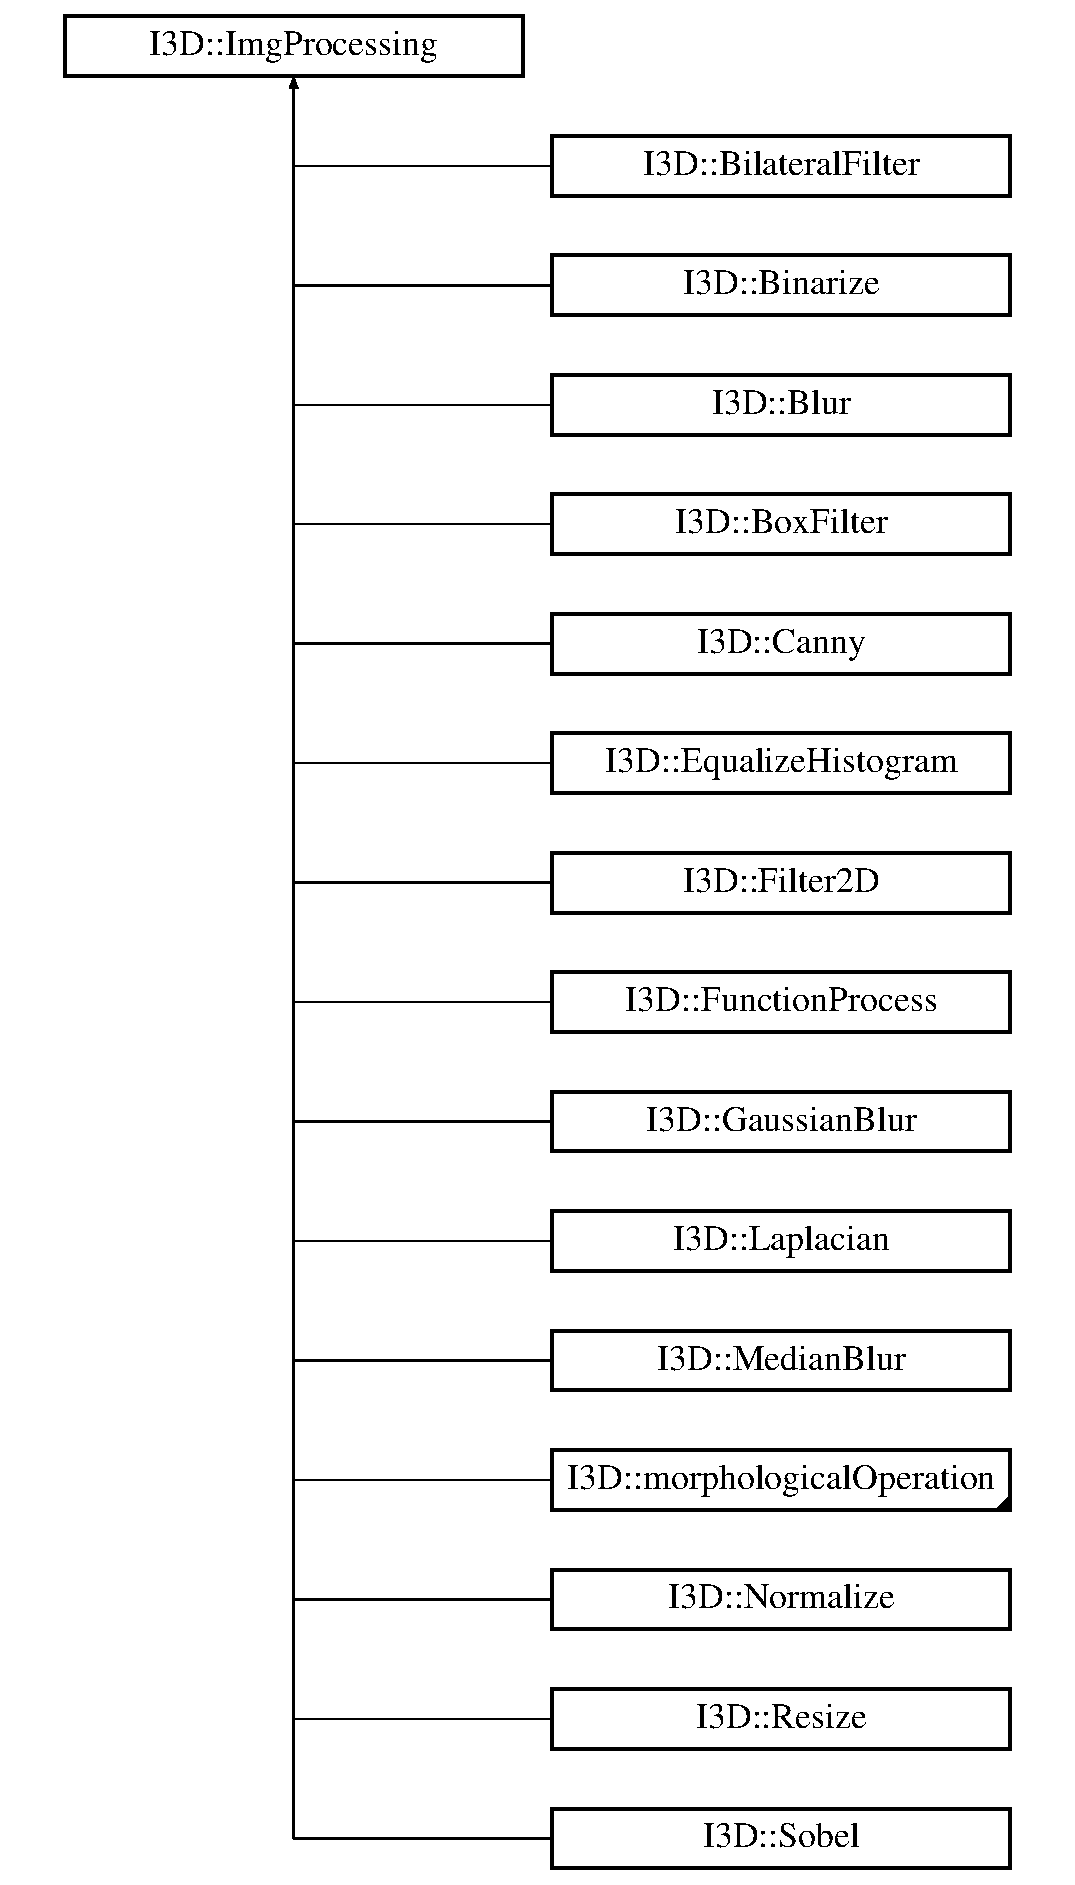
\includegraphics[height=12.000000cm]{class_i3_d_1_1_img_processing}
\end{center}
\end{figure}
\subsection*{Métodos públicos}
\begin{DoxyCompactItemize}
\item 
\hyperlink{class_i3_d_1_1_img_processing_a75646e118aa905b04ee812c477c022b6}{Img\+Processing} (\hyperlink{group___img_proc_gaa7be5aaaa0e9ec5885c5bd72f41dad47}{process\+\_\+type} \+\_\+type)
\begin{DoxyCompactList}\small\item\em Constructora de la clase. \end{DoxyCompactList}\item 
virtual \hyperlink{class_i3_d_1_1_img_processing_a5afdc256925dc91966d1d976fdf1a6bc}{$\sim$\+Img\+Processing} ()
\begin{DoxyCompactList}\small\item\em Destuctora. \end{DoxyCompactList}\item 
virtual int \hyperlink{class_i3_d_1_1_img_processing_a74195f05bbf034566e9ff6e10f3af4c9}{execute} (const cv\+::\+Mat \&mat\+In, cv\+::\+Mat $\ast$mat\+Out) const  =0
\begin{DoxyCompactList}\small\item\em Ejecuta el proceso Metodo virtual puro que deben implementar las clases hijas. \end{DoxyCompactList}\end{DoxyCompactItemize}
\subsection*{Atributos públicos}
\begin{DoxyCompactItemize}
\item 
\hyperlink{group___img_proc_gaa7be5aaaa0e9ec5885c5bd72f41dad47}{process\+\_\+type} \hyperlink{class_i3_d_1_1_img_processing_af87bd3404d91bca669b04af1f45cbff0}{type}
\begin{DoxyCompactList}\small\item\em Tipo de proceso de imagen. \end{DoxyCompactList}\end{DoxyCompactItemize}


\subsection{Descripción detallada}
Clase para gestionar los procesos de imagen Clase que permite tener una interfaz común para aplicar filtros u otros procesos a una imagen. 

\subsection{Documentación del constructor y destructor}
\index{I3\+D\+::\+Img\+Processing@{I3\+D\+::\+Img\+Processing}!Img\+Processing@{Img\+Processing}}
\index{Img\+Processing@{Img\+Processing}!I3\+D\+::\+Img\+Processing@{I3\+D\+::\+Img\+Processing}}
\subsubsection[{\texorpdfstring{Img\+Processing(process\+\_\+type \+\_\+type)}{ImgProcessing(process_type _type)}}]{\setlength{\rightskip}{0pt plus 5cm}I3\+D\+::\+Img\+Processing\+::\+Img\+Processing (
\begin{DoxyParamCaption}
\item[{{\bf process\+\_\+type}}]{\+\_\+type}
\end{DoxyParamCaption}
)\hspace{0.3cm}{\ttfamily [inline]}}\hypertarget{class_i3_d_1_1_img_processing_a75646e118aa905b04ee812c477c022b6}{}\label{class_i3_d_1_1_img_processing_a75646e118aa905b04ee812c477c022b6}


Constructora de la clase. 


\begin{DoxyParams}[1]{Parámetros}
\mbox{\tt in}  & {\em \+\_\+type} & Tipo de proceso. \\
\hline
\end{DoxyParams}
\begin{DoxySeeAlso}{Ver también}
\hyperlink{group___img_proc_gaa7be5aaaa0e9ec5885c5bd72f41dad47}{process\+\_\+type} 
\end{DoxySeeAlso}
\index{I3\+D\+::\+Img\+Processing@{I3\+D\+::\+Img\+Processing}!````~Img\+Processing@{$\sim$\+Img\+Processing}}
\index{````~Img\+Processing@{$\sim$\+Img\+Processing}!I3\+D\+::\+Img\+Processing@{I3\+D\+::\+Img\+Processing}}
\subsubsection[{\texorpdfstring{$\sim$\+Img\+Processing()}{~ImgProcessing()}}]{\setlength{\rightskip}{0pt plus 5cm}virtual I3\+D\+::\+Img\+Processing\+::$\sim$\+Img\+Processing (
\begin{DoxyParamCaption}
{}
\end{DoxyParamCaption}
)\hspace{0.3cm}{\ttfamily [inline]}, {\ttfamily [virtual]}}\hypertarget{class_i3_d_1_1_img_processing_a5afdc256925dc91966d1d976fdf1a6bc}{}\label{class_i3_d_1_1_img_processing_a5afdc256925dc91966d1d976fdf1a6bc}


Destuctora. 



\subsection{Documentación de las funciones miembro}
\index{I3\+D\+::\+Img\+Processing@{I3\+D\+::\+Img\+Processing}!execute@{execute}}
\index{execute@{execute}!I3\+D\+::\+Img\+Processing@{I3\+D\+::\+Img\+Processing}}
\subsubsection[{\texorpdfstring{execute(const cv\+::\+Mat \&mat\+In, cv\+::\+Mat $\ast$mat\+Out) const  =0}{execute(const cv::Mat &matIn, cv::Mat *matOut) const  =0}}]{\setlength{\rightskip}{0pt plus 5cm}virtual int I3\+D\+::\+Img\+Processing\+::execute (
\begin{DoxyParamCaption}
\item[{const cv\+::\+Mat \&}]{mat\+In, }
\item[{cv\+::\+Mat $\ast$}]{mat\+Out}
\end{DoxyParamCaption}
) const\hspace{0.3cm}{\ttfamily [pure virtual]}}\hypertarget{class_i3_d_1_1_img_processing_a74195f05bbf034566e9ff6e10f3af4c9}{}\label{class_i3_d_1_1_img_processing_a74195f05bbf034566e9ff6e10f3af4c9}


Ejecuta el proceso Metodo virtual puro que deben implementar las clases hijas. 


\begin{DoxyParams}[1]{Parámetros}
\mbox{\tt in}  & {\em mat\+In} & Imagen de entrada \\
\hline
\mbox{\tt out}  & {\em mat\+Out} & Imagen de salida \\
\hline
\end{DoxyParams}
\begin{DoxyReturn}{Devuelve}
Error. Si los procesos se ejecutan correctamente devuelve 0. 
\end{DoxyReturn}


Implementado en \hyperlink{class_i3_d_1_1morphological_operation_aafa533c5999bed3e9d4680a6434cb43e}{I3\+D\+::morphological\+Operation}, \hyperlink{class_i3_d_1_1_function_process_aa321eb93219271fa3f841538b61133c3}{I3\+D\+::\+Function\+Process}, \hyperlink{class_i3_d_1_1_equalize_histogram_ac748887f28d189287a120b5c6b0977a2}{I3\+D\+::\+Equalize\+Histogram}, \hyperlink{class_i3_d_1_1_resize_a683bd71d9e24c64416dc68231728a73e}{I3\+D\+::\+Resize}, \hyperlink{class_i3_d_1_1_binarize_a2630da33f5cc1c9fe80c991ffd84f613}{I3\+D\+::\+Binarize}, \hyperlink{class_i3_d_1_1_normalize_a14506e377bd5da73c37ce960c2fdf07e}{I3\+D\+::\+Normalize}, \hyperlink{class_i3_d_1_1_canny_a5337ec2dd0c95fe7c9d05444ed8f6425}{I3\+D\+::\+Canny}, \hyperlink{class_i3_d_1_1_sobel_a902c7392196e514597820fbe13a2a634}{I3\+D\+::\+Sobel}, \hyperlink{class_i3_d_1_1_median_blur_aae49eae3c8ceda4ba3a2c485d2a64b4d}{I3\+D\+::\+Median\+Blur}, \hyperlink{class_i3_d_1_1_laplacian_a7e14ea57d17b73a74058083a809fa5c3}{I3\+D\+::\+Laplacian}, \hyperlink{class_i3_d_1_1_gaussian_blur_a19812cea51167dd35e8a85d3178061d5}{I3\+D\+::\+Gaussian\+Blur}, \hyperlink{class_i3_d_1_1_filter2_d_a46f44465658be004e62d7e72cc40cb84}{I3\+D\+::\+Filter2D}, \hyperlink{class_i3_d_1_1_box_filter_aaea2d395620162626a7b16b85ae44c42}{I3\+D\+::\+Box\+Filter}, \hyperlink{class_i3_d_1_1_blur_a9bc99ea12ce16294f415f67ce467a81b}{I3\+D\+::\+Blur} y \hyperlink{class_i3_d_1_1_bilateral_filter_a4b606ce8517fbd44dd1734e1a54bab10}{I3\+D\+::\+Bilateral\+Filter}.



\subsection{Documentación de los datos miembro}
\index{I3\+D\+::\+Img\+Processing@{I3\+D\+::\+Img\+Processing}!type@{type}}
\index{type@{type}!I3\+D\+::\+Img\+Processing@{I3\+D\+::\+Img\+Processing}}
\subsubsection[{\texorpdfstring{type}{type}}]{\setlength{\rightskip}{0pt plus 5cm}{\bf process\+\_\+type} I3\+D\+::\+Img\+Processing\+::type}\hypertarget{class_i3_d_1_1_img_processing_af87bd3404d91bca669b04af1f45cbff0}{}\label{class_i3_d_1_1_img_processing_af87bd3404d91bca669b04af1f45cbff0}


Tipo de proceso de imagen. 

\begin{DoxySeeAlso}{Ver también}
\hyperlink{group___img_proc_gaa7be5aaaa0e9ec5885c5bd72f41dad47}{process\+\_\+type} 
\end{DoxySeeAlso}


La documentación para esta clase fue generada a partir del siguiente fichero\+:\begin{DoxyCompactItemize}
\item 
D\+:/\+Desarrollo/tidop/src/\hyperlink{_img_processing_8h}{Img\+Processing.\+h}\end{DoxyCompactItemize}

\hypertarget{class_i3_d_1_1_img_processing_list}{}\section{Referencia de la Clase I3D\+:\+:Img\+Processing\+List}
\label{class_i3_d_1_1_img_processing_list}\index{I3\+D\+::\+Img\+Processing\+List@{I3\+D\+::\+Img\+Processing\+List}}


Contenedor de procesos de imagen que permite su ejecución secuencial.  




{\ttfamily \#include $<$Img\+Processing.\+h$>$}

\subsection*{Métodos públicos}
\begin{DoxyCompactItemize}
\item 
\hyperlink{class_i3_d_1_1_img_processing_list_a458a291aa59116d01b89ace62e53d5e3}{Img\+Processing\+List} ()
\begin{DoxyCompactList}\small\item\em Constructora por defecto. \end{DoxyCompactList}\item 
\hyperlink{class_i3_d_1_1_img_processing_list_a72a579b6cac5bc173b882af45b7f052d}{Img\+Processing\+List} (const \hyperlink{class_i3_d_1_1_img_processing_list}{Img\+Processing\+List} \&img\+Proc\+List)
\begin{DoxyCompactList}\small\item\em Constructor de copia. \end{DoxyCompactList}\item 
\hyperlink{class_i3_d_1_1_img_processing_list_a129fcd23d97ed0c2773e97032123cb05}{Img\+Processing\+List} (std\+::initializer\+\_\+list$<$ std\+::shared\+\_\+ptr$<$ \hyperlink{class_i3_d_1_1_img_processing}{Img\+Processing} $>$$>$ img\+Proc\+List)
\begin{DoxyCompactList}\small\item\em Constructor de lista. \end{DoxyCompactList}\item 
\hyperlink{class_i3_d_1_1_img_processing_list_a7c0dc2793b201e13ee1408943bb2daa6}{$\sim$\+Img\+Processing\+List} ()
\begin{DoxyCompactList}\small\item\em Destructora. \end{DoxyCompactList}\item 
void \hyperlink{class_i3_d_1_1_img_processing_list_af0b371a633fa2c3ab77b2100e24c40ac}{add} (std\+::shared\+\_\+ptr$<$ \hyperlink{class_i3_d_1_1_img_processing}{Img\+Processing} $>$ ip)
\begin{DoxyCompactList}\small\item\em Añade un nuevo proceso a la lista. \end{DoxyCompactList}\item 
int \hyperlink{class_i3_d_1_1_img_processing_list_a4b48e25f5b7771fbdf2512c219cba4f9}{execute} (const cv\+::\+Mat \&mat\+In, cv\+::\+Mat $\ast$mat\+Out) const 
\begin{DoxyCompactList}\small\item\em Ejecuta la lista de procesos. \end{DoxyCompactList}\item 
void \hyperlink{class_i3_d_1_1_img_processing_list_a2e77f8af26c4e10ddd9d4fc2543d69e6}{clear} ()
\begin{DoxyCompactList}\small\item\em Limpia la lista de procesos. \end{DoxyCompactList}\end{DoxyCompactItemize}


\subsection{Descripción detallada}
Contenedor de procesos de imagen que permite su ejecución secuencial. 


\begin{DoxyCode}
\hyperlink{class_i3_d_1_1_img_processing_list}{I3D::ImgProcessingList} imgprolist;
imgprolist.\hyperlink{class_i3_d_1_1_img_processing_list_af0b371a633fa2c3ab77b2100e24c40ac}{add}(std::make\_shared<I3D::Normalize>(0., 255.));
imgprolist.\hyperlink{class_i3_d_1_1_img_processing_list_af0b371a633fa2c3ab77b2100e24c40ac}{add}(std::make\_shared<I3D::BilateralFilter>(5, 50., 50.));
imgprolist.\hyperlink{class_i3_d_1_1_img_processing_list_af0b371a633fa2c3ab77b2100e24c40ac}{add}(std::make\_shared<I3D::Erotion>(1));
imgprolist.\hyperlink{class_i3_d_1_1_img_processing_list_af0b371a633fa2c3ab77b2100e24c40ac}{add}(std::make\_shared<I3D::Dilate>(1));
cv::Mat out;
imgprolist.\hyperlink{class_i3_d_1_1_img_processing_list_a4b48e25f5b7771fbdf2512c219cba4f9}{execute}(in, &out);
\end{DoxyCode}
 

\subsection{Documentación del constructor y destructor}
\index{I3\+D\+::\+Img\+Processing\+List@{I3\+D\+::\+Img\+Processing\+List}!Img\+Processing\+List@{Img\+Processing\+List}}
\index{Img\+Processing\+List@{Img\+Processing\+List}!I3\+D\+::\+Img\+Processing\+List@{I3\+D\+::\+Img\+Processing\+List}}
\subsubsection[{\texorpdfstring{Img\+Processing\+List()}{ImgProcessingList()}}]{\setlength{\rightskip}{0pt plus 5cm}I3\+D\+::\+Img\+Processing\+List\+::\+Img\+Processing\+List (
\begin{DoxyParamCaption}
{}
\end{DoxyParamCaption}
)\hspace{0.3cm}{\ttfamily [inline]}}\hypertarget{class_i3_d_1_1_img_processing_list_a458a291aa59116d01b89ace62e53d5e3}{}\label{class_i3_d_1_1_img_processing_list_a458a291aa59116d01b89ace62e53d5e3}


Constructora por defecto. 

\index{I3\+D\+::\+Img\+Processing\+List@{I3\+D\+::\+Img\+Processing\+List}!Img\+Processing\+List@{Img\+Processing\+List}}
\index{Img\+Processing\+List@{Img\+Processing\+List}!I3\+D\+::\+Img\+Processing\+List@{I3\+D\+::\+Img\+Processing\+List}}
\subsubsection[{\texorpdfstring{Img\+Processing\+List(const Img\+Processing\+List \&img\+Proc\+List)}{ImgProcessingList(const ImgProcessingList &imgProcList)}}]{\setlength{\rightskip}{0pt plus 5cm}I3\+D\+::\+Img\+Processing\+List\+::\+Img\+Processing\+List (
\begin{DoxyParamCaption}
\item[{const {\bf Img\+Processing\+List} \&}]{img\+Proc\+List}
\end{DoxyParamCaption}
)\hspace{0.3cm}{\ttfamily [inline]}}\hypertarget{class_i3_d_1_1_img_processing_list_a72a579b6cac5bc173b882af45b7f052d}{}\label{class_i3_d_1_1_img_processing_list_a72a579b6cac5bc173b882af45b7f052d}


Constructor de copia. 


\begin{DoxyParams}[1]{Parámetros}
\mbox{\tt in}  & {\em img\+Proc\+List} & \hyperlink{class_i3_d_1_1_img_processing_list}{Img\+Processing\+List} que se copia \\
\hline
\end{DoxyParams}
\index{I3\+D\+::\+Img\+Processing\+List@{I3\+D\+::\+Img\+Processing\+List}!Img\+Processing\+List@{Img\+Processing\+List}}
\index{Img\+Processing\+List@{Img\+Processing\+List}!I3\+D\+::\+Img\+Processing\+List@{I3\+D\+::\+Img\+Processing\+List}}
\subsubsection[{\texorpdfstring{Img\+Processing\+List(std\+::initializer\+\_\+list$<$ std\+::shared\+\_\+ptr$<$ Img\+Processing $>$$>$ img\+Proc\+List)}{ImgProcessingList(std::initializer_list< std::shared_ptr< ImgProcessing >> imgProcList)}}]{\setlength{\rightskip}{0pt plus 5cm}I3\+D\+::\+Img\+Processing\+List\+::\+Img\+Processing\+List (
\begin{DoxyParamCaption}
\item[{std\+::initializer\+\_\+list$<$ std\+::shared\+\_\+ptr$<$ {\bf Img\+Processing} $>$$>$}]{img\+Proc\+List}
\end{DoxyParamCaption}
)\hspace{0.3cm}{\ttfamily [inline]}}\hypertarget{class_i3_d_1_1_img_processing_list_a129fcd23d97ed0c2773e97032123cb05}{}\label{class_i3_d_1_1_img_processing_list_a129fcd23d97ed0c2773e97032123cb05}


Constructor de lista. 


\begin{DoxyParams}[1]{Parámetros}
\mbox{\tt in}  & {\em Listado} & de procesos \\
\hline
\end{DoxyParams}
\index{I3\+D\+::\+Img\+Processing\+List@{I3\+D\+::\+Img\+Processing\+List}!````~Img\+Processing\+List@{$\sim$\+Img\+Processing\+List}}
\index{````~Img\+Processing\+List@{$\sim$\+Img\+Processing\+List}!I3\+D\+::\+Img\+Processing\+List@{I3\+D\+::\+Img\+Processing\+List}}
\subsubsection[{\texorpdfstring{$\sim$\+Img\+Processing\+List()}{~ImgProcessingList()}}]{\setlength{\rightskip}{0pt plus 5cm}I3\+D\+::\+Img\+Processing\+List\+::$\sim$\+Img\+Processing\+List (
\begin{DoxyParamCaption}
{}
\end{DoxyParamCaption}
)\hspace{0.3cm}{\ttfamily [inline]}}\hypertarget{class_i3_d_1_1_img_processing_list_a7c0dc2793b201e13ee1408943bb2daa6}{}\label{class_i3_d_1_1_img_processing_list_a7c0dc2793b201e13ee1408943bb2daa6}


Destructora. 



\subsection{Documentación de las funciones miembro}
\index{I3\+D\+::\+Img\+Processing\+List@{I3\+D\+::\+Img\+Processing\+List}!add@{add}}
\index{add@{add}!I3\+D\+::\+Img\+Processing\+List@{I3\+D\+::\+Img\+Processing\+List}}
\subsubsection[{\texorpdfstring{add(std\+::shared\+\_\+ptr$<$ Img\+Processing $>$ ip)}{add(std::shared_ptr< ImgProcessing > ip)}}]{\setlength{\rightskip}{0pt plus 5cm}void I3\+D\+::\+Img\+Processing\+List\+::add (
\begin{DoxyParamCaption}
\item[{std\+::shared\+\_\+ptr$<$ {\bf Img\+Processing} $>$}]{ip}
\end{DoxyParamCaption}
)}\hypertarget{class_i3_d_1_1_img_processing_list_af0b371a633fa2c3ab77b2100e24c40ac}{}\label{class_i3_d_1_1_img_processing_list_af0b371a633fa2c3ab77b2100e24c40ac}


Añade un nuevo proceso a la lista. 


\begin{DoxyParams}[1]{Parámetros}
\mbox{\tt in}  & {\em ip} & Proceso que se añade \\
\hline
\end{DoxyParams}
\index{I3\+D\+::\+Img\+Processing\+List@{I3\+D\+::\+Img\+Processing\+List}!clear@{clear}}
\index{clear@{clear}!I3\+D\+::\+Img\+Processing\+List@{I3\+D\+::\+Img\+Processing\+List}}
\subsubsection[{\texorpdfstring{clear()}{clear()}}]{\setlength{\rightskip}{0pt plus 5cm}void I3\+D\+::\+Img\+Processing\+List\+::clear (
\begin{DoxyParamCaption}
{}
\end{DoxyParamCaption}
)\hspace{0.3cm}{\ttfamily [inline]}}\hypertarget{class_i3_d_1_1_img_processing_list_a2e77f8af26c4e10ddd9d4fc2543d69e6}{}\label{class_i3_d_1_1_img_processing_list_a2e77f8af26c4e10ddd9d4fc2543d69e6}


Limpia la lista de procesos. 

\index{I3\+D\+::\+Img\+Processing\+List@{I3\+D\+::\+Img\+Processing\+List}!execute@{execute}}
\index{execute@{execute}!I3\+D\+::\+Img\+Processing\+List@{I3\+D\+::\+Img\+Processing\+List}}
\subsubsection[{\texorpdfstring{execute(const cv\+::\+Mat \&mat\+In, cv\+::\+Mat $\ast$mat\+Out) const }{execute(const cv::Mat &matIn, cv::Mat *matOut) const }}]{\setlength{\rightskip}{0pt plus 5cm}int I3\+D\+::\+Img\+Processing\+List\+::execute (
\begin{DoxyParamCaption}
\item[{const cv\+::\+Mat \&}]{mat\+In, }
\item[{cv\+::\+Mat $\ast$}]{mat\+Out}
\end{DoxyParamCaption}
) const}\hypertarget{class_i3_d_1_1_img_processing_list_a4b48e25f5b7771fbdf2512c219cba4f9}{}\label{class_i3_d_1_1_img_processing_list_a4b48e25f5b7771fbdf2512c219cba4f9}


Ejecuta la lista de procesos. 


\begin{DoxyParams}[1]{Parámetros}
\mbox{\tt in}  & {\em mat\+In} & Imagen de entrada \\
\hline
\mbox{\tt out}  & {\em mat\+Out} & Imagen de salida \\
\hline
\end{DoxyParams}
\begin{DoxyReturn}{Devuelve}
Error. Si los procesos se ejecutan correctamente devuelve 0. 
\end{DoxyReturn}


La documentación para esta clase fue generada a partir de los siguientes ficheros\+:\begin{DoxyCompactItemize}
\item 
C\+:/\+Desarrollo/tidop/src/\hyperlink{_img_processing_8h}{Img\+Processing.\+h}\item 
C\+:/\+Desarrollo/tidop/src/\hyperlink{_img_processing_8cpp}{Img\+Processing.\+cpp}\end{DoxyCompactItemize}

\hypertarget{class_i3_d_1_1_laplacian}{}\section{Referencia de la Clase I3D\+:\+:Laplacian}
\label{class_i3_d_1_1_laplacian}\index{I3\+D\+::\+Laplacian@{I3\+D\+::\+Laplacian}}


Laplaciano Calcula el laplaciano de un imagen.  




{\ttfamily \#include $<$Img\+Processing.\+h$>$}

Diagrama de herencias de I3D\+:\+:Laplacian\begin{figure}[H]
\begin{center}
\leavevmode
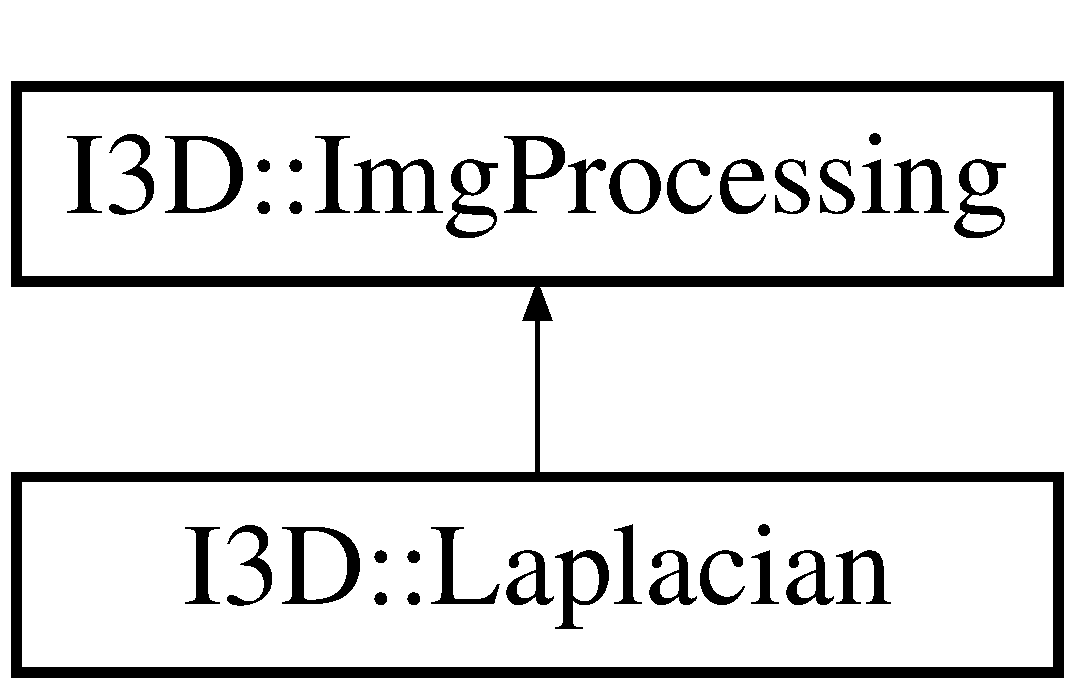
\includegraphics[height=2.000000cm]{class_i3_d_1_1_laplacian}
\end{center}
\end{figure}
\subsection*{Métodos públicos}
\begin{DoxyCompactItemize}
\item 
\hyperlink{class_i3_d_1_1_laplacian_a660abad9d6ad7cbe96544cca51d32e40}{Laplacian} (int ddepth, int ksize, double scale=1, double delta=0, int bordertype=cv\+::\+B\+O\+R\+D\+E\+R\+\_\+\+D\+E\+F\+A\+U\+LT)
\begin{DoxyCompactList}\small\item\em \hyperlink{class_i3_d_1_1_laplacian}{Laplacian}. \end{DoxyCompactList}\item 
int \hyperlink{class_i3_d_1_1_laplacian_a7e14ea57d17b73a74058083a809fa5c3}{execute} (const cv\+::\+Mat \&mat\+In, cv\+::\+Mat $\ast$mat\+Out) const  override
\begin{DoxyCompactList}\small\item\em Ejecuta el proceso. \end{DoxyCompactList}\item 
void \hyperlink{class_i3_d_1_1_laplacian_a5ac3f547a4832a13059e12941328bf58}{set\+Parameters} (int ddepth, int ksize, double scale=1, double delta=0, int bordertype=cv\+::\+B\+O\+R\+D\+E\+R\+\_\+\+D\+E\+F\+A\+U\+LT)
\begin{DoxyCompactList}\small\item\em Establece los parámetros. \end{DoxyCompactList}\end{DoxyCompactItemize}
\subsection*{Otros miembros heredados}


\subsection{Descripción detallada}
Laplaciano Calcula el laplaciano de un imagen. 

\subsection{Documentación del constructor y destructor}
\index{I3\+D\+::\+Laplacian@{I3\+D\+::\+Laplacian}!Laplacian@{Laplacian}}
\index{Laplacian@{Laplacian}!I3\+D\+::\+Laplacian@{I3\+D\+::\+Laplacian}}
\subsubsection[{\texorpdfstring{Laplacian(int ddepth, int ksize, double scale=1, double delta=0, int bordertype=cv\+::\+B\+O\+R\+D\+E\+R\+\_\+\+D\+E\+F\+A\+U\+L\+T)}{Laplacian(int ddepth, int ksize, double scale=1, double delta=0, int bordertype=cv::BORDER_DEFAULT)}}]{\setlength{\rightskip}{0pt plus 5cm}I3\+D\+::\+Laplacian\+::\+Laplacian (
\begin{DoxyParamCaption}
\item[{int}]{ddepth, }
\item[{int}]{ksize, }
\item[{double}]{scale = {\ttfamily 1}, }
\item[{double}]{delta = {\ttfamily 0}, }
\item[{int}]{bordertype = {\ttfamily cv\+:\+:BORDER\+\_\+DEFAULT}}
\end{DoxyParamCaption}
)\hspace{0.3cm}{\ttfamily [inline]}}\hypertarget{class_i3_d_1_1_laplacian_a660abad9d6ad7cbe96544cca51d32e40}{}\label{class_i3_d_1_1_laplacian_a660abad9d6ad7cbe96544cca51d32e40}


\hyperlink{class_i3_d_1_1_laplacian}{Laplacian}. 


\begin{DoxyParams}[1]{Parámetros}
\mbox{\tt in}  & {\em ddepth} & Profundidad deseada de la imagen de destino \\
\hline
\mbox{\tt in}  & {\em ksize} & Apertura del filtro \\
\hline
\mbox{\tt in}  & {\em scale} & Factor de escala opcional para los valores calculados por el laplaciano. Por defecto no se aplica escala. \\
\hline
\mbox{\tt in}  & {\em delta} & Valor opcional añadido a los píxeles filtrados \\
\hline
\mbox{\tt in}  & {\em bordertype} & Método de extrapolación (cv\+::\+Border\+Types) \\
\hline
\end{DoxyParams}


\subsection{Documentación de las funciones miembro}
\index{I3\+D\+::\+Laplacian@{I3\+D\+::\+Laplacian}!execute@{execute}}
\index{execute@{execute}!I3\+D\+::\+Laplacian@{I3\+D\+::\+Laplacian}}
\subsubsection[{\texorpdfstring{execute(const cv\+::\+Mat \&mat\+In, cv\+::\+Mat $\ast$mat\+Out) const  override}{execute(const cv::Mat &matIn, cv::Mat *matOut) const  override}}]{\setlength{\rightskip}{0pt plus 5cm}int I3\+D\+::\+Laplacian\+::execute (
\begin{DoxyParamCaption}
\item[{const cv\+::\+Mat \&}]{mat\+In, }
\item[{cv\+::\+Mat $\ast$}]{mat\+Out}
\end{DoxyParamCaption}
) const\hspace{0.3cm}{\ttfamily [override]}, {\ttfamily [virtual]}}\hypertarget{class_i3_d_1_1_laplacian_a7e14ea57d17b73a74058083a809fa5c3}{}\label{class_i3_d_1_1_laplacian_a7e14ea57d17b73a74058083a809fa5c3}


Ejecuta el proceso. 


\begin{DoxyParams}[1]{Parámetros}
\mbox{\tt in}  & {\em mat\+In} & Imagen de entrada \\
\hline
\mbox{\tt out}  & {\em mat\+Out} & Imagen de salida \\
\hline
\end{DoxyParams}
\begin{DoxyReturn}{Devuelve}
Error. Si los procesos se ejecutan correctamente devuelve 0. 
\end{DoxyReturn}


Implementa \hyperlink{class_i3_d_1_1_img_processing_a74195f05bbf034566e9ff6e10f3af4c9}{I3\+D\+::\+Img\+Processing}.

\index{I3\+D\+::\+Laplacian@{I3\+D\+::\+Laplacian}!set\+Parameters@{set\+Parameters}}
\index{set\+Parameters@{set\+Parameters}!I3\+D\+::\+Laplacian@{I3\+D\+::\+Laplacian}}
\subsubsection[{\texorpdfstring{set\+Parameters(int ddepth, int ksize, double scale=1, double delta=0, int bordertype=cv\+::\+B\+O\+R\+D\+E\+R\+\_\+\+D\+E\+F\+A\+U\+L\+T)}{setParameters(int ddepth, int ksize, double scale=1, double delta=0, int bordertype=cv::BORDER_DEFAULT)}}]{\setlength{\rightskip}{0pt plus 5cm}void I3\+D\+::\+Laplacian\+::set\+Parameters (
\begin{DoxyParamCaption}
\item[{int}]{ddepth, }
\item[{int}]{ksize, }
\item[{double}]{scale = {\ttfamily 1}, }
\item[{double}]{delta = {\ttfamily 0}, }
\item[{int}]{bordertype = {\ttfamily cv\+:\+:BORDER\+\_\+DEFAULT}}
\end{DoxyParamCaption}
)}\hypertarget{class_i3_d_1_1_laplacian_a5ac3f547a4832a13059e12941328bf58}{}\label{class_i3_d_1_1_laplacian_a5ac3f547a4832a13059e12941328bf58}


Establece los parámetros. 


\begin{DoxyParams}[1]{Parámetros}
\mbox{\tt in}  & {\em ddepth} & Profundidad deseada de la imagen de destino \\
\hline
\mbox{\tt in}  & {\em ksize} & Apertura del filtro \\
\hline
\mbox{\tt in}  & {\em scale} & Factor de escala opcional para los valores calculados por el laplaciano. Por defecto no se aplica escala. \\
\hline
\mbox{\tt in}  & {\em delta} & Valor opcional añadido a los píxeles filtrados \\
\hline
\mbox{\tt in}  & {\em bordertype} & Método de extrapolación (cv\+::\+Border\+Types) \\
\hline
\end{DoxyParams}


La documentación para esta clase fue generada a partir de los siguientes ficheros\+:\begin{DoxyCompactItemize}
\item 
C\+:/\+Desarrollo/tidop/src/\hyperlink{_img_processing_8h}{Img\+Processing.\+h}\item 
C\+:/\+Desarrollo/tidop/src/\hyperlink{_img_processing_8cpp}{Img\+Processing.\+cpp}\end{DoxyCompactItemize}

\hypertarget{class_i3_d_1_1ld_group_lines}{}\section{Referencia de la Clase I3D\+:\+:ld\+Group\+Lines}
\label{class_i3_d_1_1ld_group_lines}\index{I3\+D\+::ld\+Group\+Lines@{I3\+D\+::ld\+Group\+Lines}}


The \hyperlink{class_i3_d_1_1ld_group_lines}{ld\+Group\+Lines} class.  




{\ttfamily \#include $<$segment.\+h$>$}

\subsection*{Métodos públicos}
\begin{DoxyCompactItemize}
\item 
\hyperlink{class_i3_d_1_1ld_group_lines_a79a7dd784360a7b5fc298b3b3e234ff2}{ld\+Group\+Lines} ()
\begin{DoxyCompactList}\small\item\em Constructora Group\+Lines. \end{DoxyCompactList}\item 
\hyperlink{class_i3_d_1_1ld_group_lines_a23755b9c599ff37705e68847d7266b08}{ld\+Group\+Lines} (const std\+::vector$<$ \hyperlink{group___geometric_entities_ga483b43891a1b33d99406fdc397e9a445}{Line} $>$ \&lines)
\item 
void \hyperlink{class_i3_d_1_1ld_group_lines_aa64717716fa9a1cca52b984836ea0de8}{add} (const \hyperlink{group___geometric_entities_ga483b43891a1b33d99406fdc397e9a445}{Line} \&line)
\begin{DoxyCompactList}\small\item\em Destructora Group\+Lines. \end{DoxyCompactList}\item 
void \hyperlink{class_i3_d_1_1ld_group_lines_a3bd625014f024f8b1983921295c7e52f}{add} (const cv\+::\+Vec4i \&lvect)
\begin{DoxyCompactList}\small\item\em Añade una línea. \end{DoxyCompactList}\item 
double \hyperlink{class_i3_d_1_1ld_group_lines_aff601a6f106e048db7c8ed938c5451b4}{angle\+Mean} ()
\begin{DoxyCompactList}\small\item\em Ángulo máximo del grupo de líneas. \end{DoxyCompactList}\item 
void \hyperlink{class_i3_d_1_1ld_group_lines_ade2c47eb54c086d6db72521af395e55d}{Delete\+Line} (int id)
\item 
\hyperlink{group___geometric_entities_ga27980d94ceb3f3eb9e0c34e1fe93b073}{WindowI} \hyperlink{class_i3_d_1_1ld_group_lines_ab56438f47779a23d51a8678578debd2d}{get\+Bbox} ()
\begin{DoxyCompactList}\small\item\em Ventana envolvente del grupo de lineas. \end{DoxyCompactList}\item 
int \hyperlink{class_i3_d_1_1ld_group_lines_a10900f218dc71e1a0811b2a93ab98eba}{get\+Size} ()
\begin{DoxyCompactList}\small\item\em Número de líneas. \end{DoxyCompactList}\item 
\hyperlink{group___geometric_entities_ga483b43891a1b33d99406fdc397e9a445}{Line} \& \hyperlink{class_i3_d_1_1ld_group_lines_aa3539d62b5cbbb3ef6365b221fdff39c}{operator\mbox{[}$\,$\mbox{]}} (int id)
\begin{DoxyCompactList}\small\item\em Operador de indexación sobrecargado. \end{DoxyCompactList}\item 
const std\+::vector$<$ \hyperlink{group___geometric_entities_ga483b43891a1b33d99406fdc397e9a445}{Line} $>$ \& \hyperlink{class_i3_d_1_1ld_group_lines_abc2c5e0b7b4bd27d33c6ab5ad743088f}{get\+Lines} () const 
\end{DoxyCompactItemize}


\subsection{Descripción detallada}
The \hyperlink{class_i3_d_1_1ld_group_lines}{ld\+Group\+Lines} class. 

\subsection{Documentación del constructor y destructor}
\index{I3\+D\+::ld\+Group\+Lines@{I3\+D\+::ld\+Group\+Lines}!ld\+Group\+Lines@{ld\+Group\+Lines}}
\index{ld\+Group\+Lines@{ld\+Group\+Lines}!I3\+D\+::ld\+Group\+Lines@{I3\+D\+::ld\+Group\+Lines}}
\subsubsection[{\texorpdfstring{ld\+Group\+Lines()}{ldGroupLines()}}]{\setlength{\rightskip}{0pt plus 5cm}I3\+D\+::ld\+Group\+Lines\+::ld\+Group\+Lines (
\begin{DoxyParamCaption}
{}
\end{DoxyParamCaption}
)}\hypertarget{class_i3_d_1_1ld_group_lines_a79a7dd784360a7b5fc298b3b3e234ff2}{}\label{class_i3_d_1_1ld_group_lines_a79a7dd784360a7b5fc298b3b3e234ff2}


Constructora Group\+Lines. 

\index{I3\+D\+::ld\+Group\+Lines@{I3\+D\+::ld\+Group\+Lines}!ld\+Group\+Lines@{ld\+Group\+Lines}}
\index{ld\+Group\+Lines@{ld\+Group\+Lines}!I3\+D\+::ld\+Group\+Lines@{I3\+D\+::ld\+Group\+Lines}}
\subsubsection[{\texorpdfstring{ld\+Group\+Lines(const std\+::vector$<$ Line $>$ \&lines)}{ldGroupLines(const std::vector< Line > &lines)}}]{\setlength{\rightskip}{0pt plus 5cm}I3\+D\+::ld\+Group\+Lines\+::ld\+Group\+Lines (
\begin{DoxyParamCaption}
\item[{const std\+::vector$<$ {\bf Line} $>$ \&}]{lines}
\end{DoxyParamCaption}
)}\hypertarget{class_i3_d_1_1ld_group_lines_a23755b9c599ff37705e68847d7266b08}{}\label{class_i3_d_1_1ld_group_lines_a23755b9c599ff37705e68847d7266b08}


\subsection{Documentación de las funciones miembro}
\index{I3\+D\+::ld\+Group\+Lines@{I3\+D\+::ld\+Group\+Lines}!add@{add}}
\index{add@{add}!I3\+D\+::ld\+Group\+Lines@{I3\+D\+::ld\+Group\+Lines}}
\subsubsection[{\texorpdfstring{add(const Line \&line)}{add(const Line &line)}}]{\setlength{\rightskip}{0pt plus 5cm}void I3\+D\+::ld\+Group\+Lines\+::add (
\begin{DoxyParamCaption}
\item[{const {\bf Line} \&}]{line}
\end{DoxyParamCaption}
)}\hypertarget{class_i3_d_1_1ld_group_lines_aa64717716fa9a1cca52b984836ea0de8}{}\label{class_i3_d_1_1ld_group_lines_aa64717716fa9a1cca52b984836ea0de8}


Destructora Group\+Lines. 

Añade una línea 
\begin{DoxyParams}[1]{Parámetros}
\mbox{\tt in}  & {\em Line} & Linea \\
\hline
\end{DoxyParams}
\index{I3\+D\+::ld\+Group\+Lines@{I3\+D\+::ld\+Group\+Lines}!add@{add}}
\index{add@{add}!I3\+D\+::ld\+Group\+Lines@{I3\+D\+::ld\+Group\+Lines}}
\subsubsection[{\texorpdfstring{add(const cv\+::\+Vec4i \&lvect)}{add(const cv::Vec4i &lvect)}}]{\setlength{\rightskip}{0pt plus 5cm}void I3\+D\+::ld\+Group\+Lines\+::add (
\begin{DoxyParamCaption}
\item[{const cv\+::\+Vec4i \&}]{lvect}
\end{DoxyParamCaption}
)}\hypertarget{class_i3_d_1_1ld_group_lines_a3bd625014f024f8b1983921295c7e52f}{}\label{class_i3_d_1_1ld_group_lines_a3bd625014f024f8b1983921295c7e52f}


Añade una línea. 


\begin{DoxyParams}[1]{Parámetros}
\mbox{\tt in}  & {\em lvect} & \\
\hline
\end{DoxyParams}
\index{I3\+D\+::ld\+Group\+Lines@{I3\+D\+::ld\+Group\+Lines}!angle\+Mean@{angle\+Mean}}
\index{angle\+Mean@{angle\+Mean}!I3\+D\+::ld\+Group\+Lines@{I3\+D\+::ld\+Group\+Lines}}
\subsubsection[{\texorpdfstring{angle\+Mean()}{angleMean()}}]{\setlength{\rightskip}{0pt plus 5cm}double I3\+D\+::ld\+Group\+Lines\+::angle\+Mean (
\begin{DoxyParamCaption}
{}
\end{DoxyParamCaption}
)}\hypertarget{class_i3_d_1_1ld_group_lines_aff601a6f106e048db7c8ed938c5451b4}{}\label{class_i3_d_1_1ld_group_lines_aff601a6f106e048db7c8ed938c5451b4}


Ángulo máximo del grupo de líneas. 

\begin{DoxyReturn}{Devuelve}

\end{DoxyReturn}
Ángulo mínimo del grupo de líneas \begin{DoxyReturn}{Devuelve}

\end{DoxyReturn}
Ángulo medio \begin{DoxyReturn}{Devuelve}

\end{DoxyReturn}
\index{I3\+D\+::ld\+Group\+Lines@{I3\+D\+::ld\+Group\+Lines}!Delete\+Line@{Delete\+Line}}
\index{Delete\+Line@{Delete\+Line}!I3\+D\+::ld\+Group\+Lines@{I3\+D\+::ld\+Group\+Lines}}
\subsubsection[{\texorpdfstring{Delete\+Line(int id)}{DeleteLine(int id)}}]{\setlength{\rightskip}{0pt plus 5cm}void I3\+D\+::ld\+Group\+Lines\+::\+Delete\+Line (
\begin{DoxyParamCaption}
\item[{int}]{id}
\end{DoxyParamCaption}
)}\hypertarget{class_i3_d_1_1ld_group_lines_ade2c47eb54c086d6db72521af395e55d}{}\label{class_i3_d_1_1ld_group_lines_ade2c47eb54c086d6db72521af395e55d}
\index{I3\+D\+::ld\+Group\+Lines@{I3\+D\+::ld\+Group\+Lines}!get\+Bbox@{get\+Bbox}}
\index{get\+Bbox@{get\+Bbox}!I3\+D\+::ld\+Group\+Lines@{I3\+D\+::ld\+Group\+Lines}}
\subsubsection[{\texorpdfstring{get\+Bbox()}{getBbox()}}]{\setlength{\rightskip}{0pt plus 5cm}{\bf WindowI} I3\+D\+::ld\+Group\+Lines\+::get\+Bbox (
\begin{DoxyParamCaption}
{}
\end{DoxyParamCaption}
)\hspace{0.3cm}{\ttfamily [inline]}}\hypertarget{class_i3_d_1_1ld_group_lines_ab56438f47779a23d51a8678578debd2d}{}\label{class_i3_d_1_1ld_group_lines_ab56438f47779a23d51a8678578debd2d}


Ventana envolvente del grupo de lineas. 

\begin{DoxyReturn}{Devuelve}

\end{DoxyReturn}
\index{I3\+D\+::ld\+Group\+Lines@{I3\+D\+::ld\+Group\+Lines}!get\+Lines@{get\+Lines}}
\index{get\+Lines@{get\+Lines}!I3\+D\+::ld\+Group\+Lines@{I3\+D\+::ld\+Group\+Lines}}
\subsubsection[{\texorpdfstring{get\+Lines() const }{getLines() const }}]{\setlength{\rightskip}{0pt plus 5cm}const std\+::vector$<${\bf Line}$>$\& I3\+D\+::ld\+Group\+Lines\+::get\+Lines (
\begin{DoxyParamCaption}
{}
\end{DoxyParamCaption}
) const\hspace{0.3cm}{\ttfamily [inline]}}\hypertarget{class_i3_d_1_1ld_group_lines_abc2c5e0b7b4bd27d33c6ab5ad743088f}{}\label{class_i3_d_1_1ld_group_lines_abc2c5e0b7b4bd27d33c6ab5ad743088f}
\index{I3\+D\+::ld\+Group\+Lines@{I3\+D\+::ld\+Group\+Lines}!get\+Size@{get\+Size}}
\index{get\+Size@{get\+Size}!I3\+D\+::ld\+Group\+Lines@{I3\+D\+::ld\+Group\+Lines}}
\subsubsection[{\texorpdfstring{get\+Size()}{getSize()}}]{\setlength{\rightskip}{0pt plus 5cm}int I3\+D\+::ld\+Group\+Lines\+::get\+Size (
\begin{DoxyParamCaption}
{}
\end{DoxyParamCaption}
)\hspace{0.3cm}{\ttfamily [inline]}}\hypertarget{class_i3_d_1_1ld_group_lines_a10900f218dc71e1a0811b2a93ab98eba}{}\label{class_i3_d_1_1ld_group_lines_a10900f218dc71e1a0811b2a93ab98eba}


Número de líneas. 

\begin{DoxyReturn}{Devuelve}

\end{DoxyReturn}
\index{I3\+D\+::ld\+Group\+Lines@{I3\+D\+::ld\+Group\+Lines}!operator\mbox{[}$\,$\mbox{]}@{operator[]}}
\index{operator\mbox{[}$\,$\mbox{]}@{operator[]}!I3\+D\+::ld\+Group\+Lines@{I3\+D\+::ld\+Group\+Lines}}
\subsubsection[{\texorpdfstring{operator[](int id)}{operator[](int id)}}]{\setlength{\rightskip}{0pt plus 5cm}{\bf Line}\& I3\+D\+::ld\+Group\+Lines\+::operator\mbox{[}$\,$\mbox{]} (
\begin{DoxyParamCaption}
\item[{int}]{id}
\end{DoxyParamCaption}
)\hspace{0.3cm}{\ttfamily [inline]}}\hypertarget{class_i3_d_1_1ld_group_lines_aa3539d62b5cbbb3ef6365b221fdff39c}{}\label{class_i3_d_1_1ld_group_lines_aa3539d62b5cbbb3ef6365b221fdff39c}


Operador de indexación sobrecargado. 


\begin{DoxyParams}[1]{Parámetros}
\mbox{\tt in}  & {\em id} & Indice del elemento \\
\hline
\end{DoxyParams}
\begin{DoxyReturn}{Devuelve}
Linea 
\end{DoxyReturn}


La documentación para esta clase fue generada a partir de los siguientes ficheros\+:\begin{DoxyCompactItemize}
\item 
D\+:/\+Desarrollo/tidop/src/geometric\+\_\+entities/\hyperlink{segment_8h}{segment.\+h}\item 
D\+:/\+Desarrollo/tidop/src/geometric\+\_\+entities/\hyperlink{segment_8cpp}{segment.\+cpp}\end{DoxyCompactItemize}

\hypertarget{class_i3_d_1_1ld_houh}{}\section{Referencia de la Clase I3D\+:\+:ld\+Houh}
\label{class_i3_d_1_1ld_houh}\index{I3\+D\+::ld\+Houh@{I3\+D\+::ld\+Houh}}


Detector de lineas Hough.  




{\ttfamily \#include $<$Line\+Detector.\+h$>$}

Diagrama de herencias de I3D\+:\+:ld\+Houh\begin{figure}[H]
\begin{center}
\leavevmode
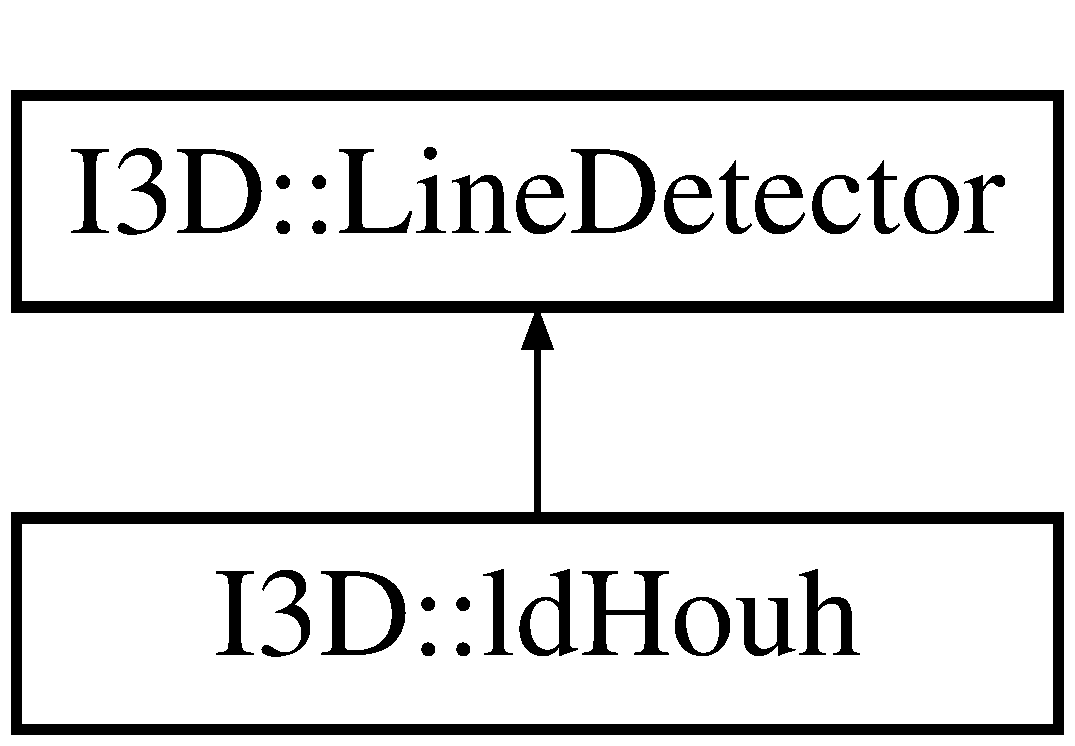
\includegraphics[height=2.000000cm]{class_i3_d_1_1ld_houh}
\end{center}
\end{figure}
\subsection*{Métodos públicos}
\begin{DoxyCompactItemize}
\item 
\hyperlink{class_i3_d_1_1ld_houh_ad9387cc250dc409bd8ab5e0768f0e8fb}{ld\+Houh} (int threshold=50, const cv\+::\+Scalar \&at=cv\+::\+Scalar(0, C\+V\+\_\+\+PI/2))
\begin{DoxyCompactList}\small\item\em Constructora de la clase \hyperlink{class_i3_d_1_1ld_houh}{ld\+Houh}. \end{DoxyCompactList}\item 
\hyperlink{class_i3_d_1_1ld_houh_a2f0c3dd6be7e15fc7fcafdbbf0520cf8}{$\sim$ld\+Houh} ()
\begin{DoxyCompactList}\small\item\em Destructora de la clase \hyperlink{class_i3_d_1_1ld_houh}{ld\+Houh}. \end{DoxyCompactList}\item 
int \hyperlink{class_i3_d_1_1ld_houh_a17c6836029eeb9448e6bd661c1aac16c}{run} (cv\+::\+Mat \&image) override
\begin{DoxyCompactList}\small\item\em Calcula la transformada de Hough para lineas. \end{DoxyCompactList}\item 
int \hyperlink{class_i3_d_1_1ld_houh_a548494c74a114c679ddc050dc9fd991a}{run} (cv\+::\+Mat \&image, const cv\+::\+Scalar \&angletol) override
\begin{DoxyCompactList}\small\item\em Calcula la transformada de Hough para lineas. \end{DoxyCompactList}\item 
void \hyperlink{class_i3_d_1_1ld_houh_ae7652d43e53ac59b4bdbca7fd2de3bdb}{set\+Threshold} (int threshold)
\begin{DoxyCompactList}\small\item\em Establece el valor de threshold. \end{DoxyCompactList}\end{DoxyCompactItemize}
\subsection*{Otros miembros heredados}


\subsection{Descripción detallada}
Detector de lineas Hough. 

Clase para la detección de lineas mediante la transformada de Hough para lineas. 

\subsection{Documentación del constructor y destructor}
\index{I3\+D\+::ld\+Houh@{I3\+D\+::ld\+Houh}!ld\+Houh@{ld\+Houh}}
\index{ld\+Houh@{ld\+Houh}!I3\+D\+::ld\+Houh@{I3\+D\+::ld\+Houh}}
\subsubsection[{\texorpdfstring{ld\+Houh(int threshold=50, const cv\+::\+Scalar \&at=cv\+::\+Scalar(0, C\+V\+\_\+\+P\+I/2))}{ldHouh(int threshold=50, const cv::Scalar &at=cv::Scalar(0, CV_PI/2))}}]{\setlength{\rightskip}{0pt plus 5cm}I3\+D\+::ld\+Houh\+::ld\+Houh (
\begin{DoxyParamCaption}
\item[{int}]{threshold = {\ttfamily 50}, }
\item[{const cv\+::\+Scalar \&}]{at = {\ttfamily cv\+:\+:Scalar(0,~CV\+\_\+PI~/~2)}}
\end{DoxyParamCaption}
)\hspace{0.3cm}{\ttfamily [inline]}}\hypertarget{class_i3_d_1_1ld_houh_ad9387cc250dc409bd8ab5e0768f0e8fb}{}\label{class_i3_d_1_1ld_houh_ad9387cc250dc409bd8ab5e0768f0e8fb}


Constructora de la clase \hyperlink{class_i3_d_1_1ld_houh}{ld\+Houh}. 


\begin{DoxyParams}[1]{Parámetros}
\mbox{\tt in}  & {\em threshold} & \\
\hline
\mbox{\tt in}  & {\em at} & Angulo y tolerancia \\
\hline
\end{DoxyParams}
\index{I3\+D\+::ld\+Houh@{I3\+D\+::ld\+Houh}!````~ld\+Houh@{$\sim$ld\+Houh}}
\index{````~ld\+Houh@{$\sim$ld\+Houh}!I3\+D\+::ld\+Houh@{I3\+D\+::ld\+Houh}}
\subsubsection[{\texorpdfstring{$\sim$ld\+Houh()}{~ldHouh()}}]{\setlength{\rightskip}{0pt plus 5cm}I3\+D\+::ld\+Houh\+::$\sim$ld\+Houh (
\begin{DoxyParamCaption}
{}
\end{DoxyParamCaption}
)\hspace{0.3cm}{\ttfamily [inline]}}\hypertarget{class_i3_d_1_1ld_houh_a2f0c3dd6be7e15fc7fcafdbbf0520cf8}{}\label{class_i3_d_1_1ld_houh_a2f0c3dd6be7e15fc7fcafdbbf0520cf8}


Destructora de la clase \hyperlink{class_i3_d_1_1ld_houh}{ld\+Houh}. 



\subsection{Documentación de las funciones miembro}
\index{I3\+D\+::ld\+Houh@{I3\+D\+::ld\+Houh}!run@{run}}
\index{run@{run}!I3\+D\+::ld\+Houh@{I3\+D\+::ld\+Houh}}
\subsubsection[{\texorpdfstring{run(cv\+::\+Mat \&image) override}{run(cv::Mat &image) override}}]{\setlength{\rightskip}{0pt plus 5cm}int I3\+D\+::ld\+Houh\+::run (
\begin{DoxyParamCaption}
\item[{cv\+::\+Mat \&}]{image}
\end{DoxyParamCaption}
)\hspace{0.3cm}{\ttfamily [override]}, {\ttfamily [virtual]}}\hypertarget{class_i3_d_1_1ld_houh_a17c6836029eeb9448e6bd661c1aac16c}{}\label{class_i3_d_1_1ld_houh_a17c6836029eeb9448e6bd661c1aac16c}


Calcula la transformada de Hough para lineas. 


\begin{DoxyParams}[1]{Parámetros}
\mbox{\tt in}  & {\em image} & Imagen en la cual se quieren detectar las lineas. \\
\hline
\end{DoxyParams}
\begin{DoxyReturn}{Devuelve}
Error 
\end{DoxyReturn}


Implementa \hyperlink{class_i3_d_1_1_line_detector_ad439cb59972938259f6b36bcdbb644b7}{I3\+D\+::\+Line\+Detector}.

\index{I3\+D\+::ld\+Houh@{I3\+D\+::ld\+Houh}!run@{run}}
\index{run@{run}!I3\+D\+::ld\+Houh@{I3\+D\+::ld\+Houh}}
\subsubsection[{\texorpdfstring{run(cv\+::\+Mat \&image, const cv\+::\+Scalar \&angletol) override}{run(cv::Mat &image, const cv::Scalar &angletol) override}}]{\setlength{\rightskip}{0pt plus 5cm}int I3\+D\+::ld\+Houh\+::run (
\begin{DoxyParamCaption}
\item[{cv\+::\+Mat \&}]{image, }
\item[{const cv\+::\+Scalar \&}]{angletol}
\end{DoxyParamCaption}
)\hspace{0.3cm}{\ttfamily [override]}, {\ttfamily [virtual]}}\hypertarget{class_i3_d_1_1ld_houh_a548494c74a114c679ddc050dc9fd991a}{}\label{class_i3_d_1_1ld_houh_a548494c74a114c679ddc050dc9fd991a}


Calcula la transformada de Hough para lineas. 


\begin{DoxyParams}[1]{Parámetros}
\mbox{\tt in}  & {\em image} & Imagen en la cual se quieren detectar las lineas \\
\hline
\mbox{\tt in}  & {\em angletol} & Angulo y tolerancia \\
\hline
\end{DoxyParams}
\begin{DoxyReturn}{Devuelve}
Error 
\end{DoxyReturn}


Implementa \hyperlink{class_i3_d_1_1_line_detector_abc00c6e15e2386a32720886d60a20ccd}{I3\+D\+::\+Line\+Detector}.

\index{I3\+D\+::ld\+Houh@{I3\+D\+::ld\+Houh}!set\+Threshold@{set\+Threshold}}
\index{set\+Threshold@{set\+Threshold}!I3\+D\+::ld\+Houh@{I3\+D\+::ld\+Houh}}
\subsubsection[{\texorpdfstring{set\+Threshold(int threshold)}{setThreshold(int threshold)}}]{\setlength{\rightskip}{0pt plus 5cm}void I3\+D\+::ld\+Houh\+::set\+Threshold (
\begin{DoxyParamCaption}
\item[{int}]{threshold}
\end{DoxyParamCaption}
)\hspace{0.3cm}{\ttfamily [inline]}}\hypertarget{class_i3_d_1_1ld_houh_ae7652d43e53ac59b4bdbca7fd2de3bdb}{}\label{class_i3_d_1_1ld_houh_ae7652d43e53ac59b4bdbca7fd2de3bdb}


Establece el valor de threshold. 


\begin{DoxyParams}[1]{Parámetros}
\mbox{\tt in}  & {\em threshold} & threshold \\
\hline
\end{DoxyParams}


La documentación para esta clase fue generada a partir de los siguientes ficheros\+:\begin{DoxyCompactItemize}
\item 
D\+:/\+Desarrollo/tidop/src/\hyperlink{_line_detector_8h}{Line\+Detector.\+h}\item 
D\+:/\+Desarrollo/tidop/src/\hyperlink{linedetector_8cpp}{linedetector.\+cpp}\end{DoxyCompactItemize}

\hypertarget{class_i3_d_1_1ld_houh_fast}{}\section{Referencia de la Clase I3D\+:\+:ld\+Houh\+Fast}
\label{class_i3_d_1_1ld_houh_fast}\index{I3\+D\+::ld\+Houh\+Fast@{I3\+D\+::ld\+Houh\+Fast}}


Detector de lineas rapido de Hough.  




{\ttfamily \#include $<$Line\+Detector.\+h$>$}

Diagrama de herencias de I3D\+:\+:ld\+Houh\+Fast\begin{figure}[H]
\begin{center}
\leavevmode
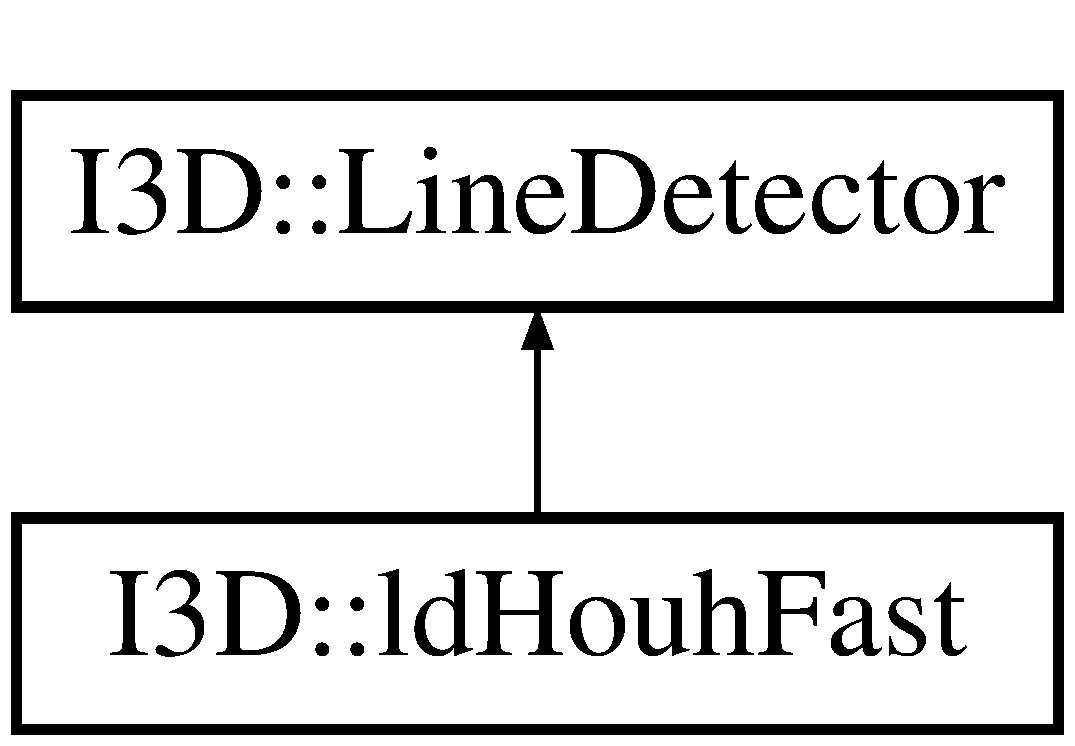
\includegraphics[height=2.000000cm]{class_i3_d_1_1ld_houh_fast}
\end{center}
\end{figure}
\subsection*{Métodos públicos}
\begin{DoxyCompactItemize}
\item 
\hyperlink{class_i3_d_1_1ld_houh_fast_a750f01c43402983b0839ba47271a2dad}{ld\+Houh\+Fast} (const cv\+::\+Scalar \&at=cv\+::\+Scalar(0, C\+V\+\_\+\+PI/2))
\begin{DoxyCompactList}\small\item\em Constructora de la clase \hyperlink{class_i3_d_1_1ld_houh_fast}{ld\+Houh\+Fast}. \end{DoxyCompactList}\item 
\hyperlink{class_i3_d_1_1ld_houh_fast_abe17675e0e7f4aec0c9400f39a8e6963}{$\sim$ld\+Houh\+Fast} ()
\begin{DoxyCompactList}\small\item\em Destructora de la clase \hyperlink{class_i3_d_1_1ld_houh_p}{ld\+HouhP}. \end{DoxyCompactList}\item 
int \hyperlink{class_i3_d_1_1ld_houh_fast_a9cbcde2e4327ba3fd7c65d404bea5ee7}{run} (cv\+::\+Mat \&image) override
\begin{DoxyCompactList}\small\item\em Calcula la transformada de Hough probabilistica para lineas. \end{DoxyCompactList}\item 
int \hyperlink{class_i3_d_1_1ld_houh_fast_a41fd58bdeeb31893f4a98a90ce9ec516}{run} (cv\+::\+Mat \&image, const cv\+::\+Scalar \&angletol) override
\begin{DoxyCompactList}\small\item\em Calcula la transformada de Hough probabilistica para lineas. \end{DoxyCompactList}\item 
void \hyperlink{class_i3_d_1_1ld_houh_fast_a514054f1d58cff2d65f3b63f3dc67e32}{set\+Parameters} ()
\begin{DoxyCompactList}\small\item\em Establece los parámetros. \end{DoxyCompactList}\end{DoxyCompactItemize}
\subsection*{Otros miembros heredados}


\subsection{Descripción detallada}
Detector de lineas rapido de Hough. 

Clase para la detección de lineas mediante la transformada rapida de Hough para lineas. Extraido de ximgproc\textbackslash{}samples\textbackslash{}fast\+\_\+hough\+\_\+transform.\+cpp 

\subsection{Documentación del constructor y destructor}
\index{I3\+D\+::ld\+Houh\+Fast@{I3\+D\+::ld\+Houh\+Fast}!ld\+Houh\+Fast@{ld\+Houh\+Fast}}
\index{ld\+Houh\+Fast@{ld\+Houh\+Fast}!I3\+D\+::ld\+Houh\+Fast@{I3\+D\+::ld\+Houh\+Fast}}
\subsubsection[{\texorpdfstring{ld\+Houh\+Fast(const cv\+::\+Scalar \&at=cv\+::\+Scalar(0, C\+V\+\_\+\+P\+I/2))}{ldHouhFast(const cv::Scalar &at=cv::Scalar(0, CV_PI/2))}}]{\setlength{\rightskip}{0pt plus 5cm}I3\+D\+::ld\+Houh\+Fast\+::ld\+Houh\+Fast (
\begin{DoxyParamCaption}
\item[{const cv\+::\+Scalar \&}]{at = {\ttfamily cv\+:\+:Scalar(0,~CV\+\_\+PI~/~2)}}
\end{DoxyParamCaption}
)\hspace{0.3cm}{\ttfamily [inline]}}\hypertarget{class_i3_d_1_1ld_houh_fast_a750f01c43402983b0839ba47271a2dad}{}\label{class_i3_d_1_1ld_houh_fast_a750f01c43402983b0839ba47271a2dad}


Constructora de la clase \hyperlink{class_i3_d_1_1ld_houh_fast}{ld\+Houh\+Fast}. 


\begin{DoxyParams}[1]{Parámetros}
\mbox{\tt in}  & {\em at} & Angulo y tolerancia \\
\hline
\end{DoxyParams}
\index{I3\+D\+::ld\+Houh\+Fast@{I3\+D\+::ld\+Houh\+Fast}!````~ld\+Houh\+Fast@{$\sim$ld\+Houh\+Fast}}
\index{````~ld\+Houh\+Fast@{$\sim$ld\+Houh\+Fast}!I3\+D\+::ld\+Houh\+Fast@{I3\+D\+::ld\+Houh\+Fast}}
\subsubsection[{\texorpdfstring{$\sim$ld\+Houh\+Fast()}{~ldHouhFast()}}]{\setlength{\rightskip}{0pt plus 5cm}I3\+D\+::ld\+Houh\+Fast\+::$\sim$ld\+Houh\+Fast (
\begin{DoxyParamCaption}
{}
\end{DoxyParamCaption}
)\hspace{0.3cm}{\ttfamily [inline]}}\hypertarget{class_i3_d_1_1ld_houh_fast_abe17675e0e7f4aec0c9400f39a8e6963}{}\label{class_i3_d_1_1ld_houh_fast_abe17675e0e7f4aec0c9400f39a8e6963}


Destructora de la clase \hyperlink{class_i3_d_1_1ld_houh_p}{ld\+HouhP}. 



\subsection{Documentación de las funciones miembro}
\index{I3\+D\+::ld\+Houh\+Fast@{I3\+D\+::ld\+Houh\+Fast}!run@{run}}
\index{run@{run}!I3\+D\+::ld\+Houh\+Fast@{I3\+D\+::ld\+Houh\+Fast}}
\subsubsection[{\texorpdfstring{run(cv\+::\+Mat \&image) override}{run(cv::Mat &image) override}}]{\setlength{\rightskip}{0pt plus 5cm}int I3\+D\+::ld\+Houh\+Fast\+::run (
\begin{DoxyParamCaption}
\item[{cv\+::\+Mat \&}]{image}
\end{DoxyParamCaption}
)\hspace{0.3cm}{\ttfamily [override]}, {\ttfamily [virtual]}}\hypertarget{class_i3_d_1_1ld_houh_fast_a9cbcde2e4327ba3fd7c65d404bea5ee7}{}\label{class_i3_d_1_1ld_houh_fast_a9cbcde2e4327ba3fd7c65d404bea5ee7}


Calcula la transformada de Hough probabilistica para lineas. 


\begin{DoxyParams}[1]{Parámetros}
\mbox{\tt in}  & {\em image} & Imagen en la cual se quieren detectar las lineas. \\
\hline
\end{DoxyParams}
\begin{DoxyReturn}{Devuelve}
Error 
\end{DoxyReturn}


Implementa \hyperlink{class_i3_d_1_1_line_detector_ad439cb59972938259f6b36bcdbb644b7}{I3\+D\+::\+Line\+Detector}.

\index{I3\+D\+::ld\+Houh\+Fast@{I3\+D\+::ld\+Houh\+Fast}!run@{run}}
\index{run@{run}!I3\+D\+::ld\+Houh\+Fast@{I3\+D\+::ld\+Houh\+Fast}}
\subsubsection[{\texorpdfstring{run(cv\+::\+Mat \&image, const cv\+::\+Scalar \&angletol) override}{run(cv::Mat &image, const cv::Scalar &angletol) override}}]{\setlength{\rightskip}{0pt plus 5cm}int I3\+D\+::ld\+Houh\+Fast\+::run (
\begin{DoxyParamCaption}
\item[{cv\+::\+Mat \&}]{image, }
\item[{const cv\+::\+Scalar \&}]{angletol}
\end{DoxyParamCaption}
)\hspace{0.3cm}{\ttfamily [override]}, {\ttfamily [virtual]}}\hypertarget{class_i3_d_1_1ld_houh_fast_a41fd58bdeeb31893f4a98a90ce9ec516}{}\label{class_i3_d_1_1ld_houh_fast_a41fd58bdeeb31893f4a98a90ce9ec516}


Calcula la transformada de Hough probabilistica para lineas. 


\begin{DoxyParams}[1]{Parámetros}
\mbox{\tt in}  & {\em image} & Imagen en la cual se quieren detectar las lineas. \\
\hline
\mbox{\tt in}  & {\em angletol} & Angulo y tolerancia \\
\hline
\end{DoxyParams}
\begin{DoxyReturn}{Devuelve}
Error 
\end{DoxyReturn}


Implementa \hyperlink{class_i3_d_1_1_line_detector_abc00c6e15e2386a32720886d60a20ccd}{I3\+D\+::\+Line\+Detector}.

\index{I3\+D\+::ld\+Houh\+Fast@{I3\+D\+::ld\+Houh\+Fast}!set\+Parameters@{set\+Parameters}}
\index{set\+Parameters@{set\+Parameters}!I3\+D\+::ld\+Houh\+Fast@{I3\+D\+::ld\+Houh\+Fast}}
\subsubsection[{\texorpdfstring{set\+Parameters()}{setParameters()}}]{\setlength{\rightskip}{0pt plus 5cm}void I3\+D\+::ld\+Houh\+Fast\+::set\+Parameters (
\begin{DoxyParamCaption}
{}
\end{DoxyParamCaption}
)}\hypertarget{class_i3_d_1_1ld_houh_fast_a514054f1d58cff2d65f3b63f3dc67e32}{}\label{class_i3_d_1_1ld_houh_fast_a514054f1d58cff2d65f3b63f3dc67e32}


Establece los parámetros. 



La documentación para esta clase fue generada a partir de los siguientes ficheros\+:\begin{DoxyCompactItemize}
\item 
C\+:/\+Desarrollo/tidop/src/\hyperlink{_line_detector_8h}{Line\+Detector.\+h}\item 
C\+:/\+Desarrollo/tidop/src/\hyperlink{linedetector_8cpp}{linedetector.\+cpp}\end{DoxyCompactItemize}

\hypertarget{class_i3_d_1_1ld_houh_p}{}\section{Referencia de la Clase I3D\+:\+:ld\+HouhP}
\label{class_i3_d_1_1ld_houh_p}\index{I3\+D\+::ld\+HouhP@{I3\+D\+::ld\+HouhP}}


Detector de lineas Hough probabilistico.  




{\ttfamily \#include $<$Line\+Detector.\+h$>$}

Diagrama de herencias de I3D\+:\+:ld\+HouhP\begin{figure}[H]
\begin{center}
\leavevmode
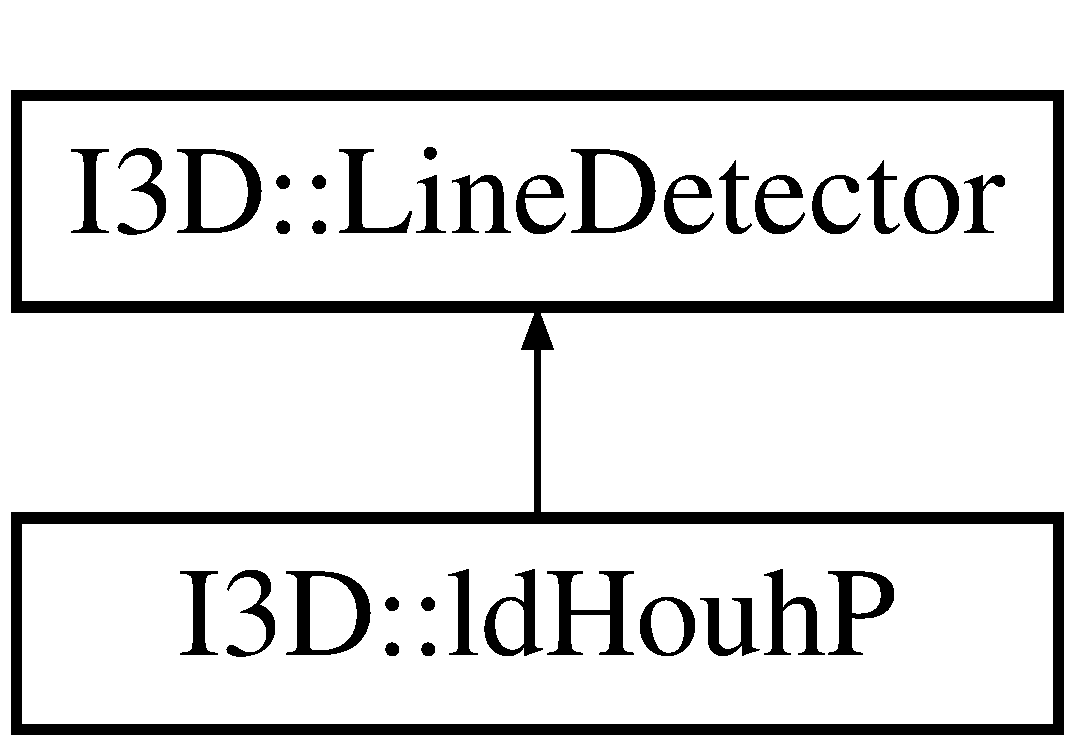
\includegraphics[height=2.000000cm]{class_i3_d_1_1ld_houh_p}
\end{center}
\end{figure}
\subsection*{Métodos públicos}
\begin{DoxyCompactItemize}
\item 
\hyperlink{class_i3_d_1_1ld_houh_p_af281fdf68e939e11d7b26238e5448535}{ld\+HouhP} (int threshold=50, const cv\+::\+Scalar \&at=cv\+::\+Scalar(0, C\+V\+\_\+\+PI/2), double min\+Line\+Length=0., double max\+Line\+Gap=0.)
\begin{DoxyCompactList}\small\item\em Constructora de la clase \hyperlink{class_i3_d_1_1ld_houh_p}{ld\+HouhP}. \end{DoxyCompactList}\item 
\hyperlink{class_i3_d_1_1ld_houh_p_a591bddef725072413c1eb3a490fb4bcf}{$\sim$ld\+HouhP} ()
\begin{DoxyCompactList}\small\item\em Destructora de la clase \hyperlink{class_i3_d_1_1ld_houh_p}{ld\+HouhP}. \end{DoxyCompactList}\item 
int \hyperlink{class_i3_d_1_1ld_houh_p_a91b42a50eb80dfcb9f5cf1bdf0d8c908}{run} (cv\+::\+Mat \&image) override
\begin{DoxyCompactList}\small\item\em Calcula la transformada de Hough probabilistica para lineas. \end{DoxyCompactList}\item 
int \hyperlink{class_i3_d_1_1ld_houh_p_ad00dcfc80128ea426b2fff2878c7e723}{run} (cv\+::\+Mat \&image, const cv\+::\+Scalar \&angletol) override
\begin{DoxyCompactList}\small\item\em Calcula la transformada de Hough probabilistica para lineas. \end{DoxyCompactList}\item 
void \hyperlink{class_i3_d_1_1ld_houh_p_a782e9ee0c5448b23e545893bf1ab564e}{set\+Threshold} (int threshold)
\begin{DoxyCompactList}\small\item\em Establece el valor de threshold. \end{DoxyCompactList}\item 
void \hyperlink{class_i3_d_1_1ld_houh_p_a0e5b764154bd17ec13d20194dedc3df4}{set\+Parameters} (double min\+Line\+Length=0., double max\+Line\+Gap=0.)
\begin{DoxyCompactList}\small\item\em Establece los parámetros. \end{DoxyCompactList}\end{DoxyCompactItemize}
\subsection*{Otros miembros heredados}


\subsection{Descripción detallada}
Detector de lineas Hough probabilistico. 

Clase para la detección de lineas mediante la transformada probabilística de Hough para lineas. 

\subsection{Documentación del constructor y destructor}
\index{I3\+D\+::ld\+HouhP@{I3\+D\+::ld\+HouhP}!ld\+HouhP@{ld\+HouhP}}
\index{ld\+HouhP@{ld\+HouhP}!I3\+D\+::ld\+HouhP@{I3\+D\+::ld\+HouhP}}
\subsubsection[{\texorpdfstring{ld\+Houh\+P(int threshold=50, const cv\+::\+Scalar \&at=cv\+::\+Scalar(0, C\+V\+\_\+\+P\+I/2), double min\+Line\+Length=0., double max\+Line\+Gap=0.)}{ldHouhP(int threshold=50, const cv::Scalar &at=cv::Scalar(0, CV_PI/2), double minLineLength=0., double maxLineGap=0.)}}]{\setlength{\rightskip}{0pt plus 5cm}I3\+D\+::ld\+Houh\+P\+::ld\+HouhP (
\begin{DoxyParamCaption}
\item[{int}]{threshold = {\ttfamily 50}, }
\item[{const cv\+::\+Scalar \&}]{at = {\ttfamily cv\+:\+:Scalar(0,~CV\+\_\+PI~/~2)}, }
\item[{double}]{min\+Line\+Length = {\ttfamily 0.}, }
\item[{double}]{max\+Line\+Gap = {\ttfamily 0.}}
\end{DoxyParamCaption}
)\hspace{0.3cm}{\ttfamily [inline]}}\hypertarget{class_i3_d_1_1ld_houh_p_af281fdf68e939e11d7b26238e5448535}{}\label{class_i3_d_1_1ld_houh_p_af281fdf68e939e11d7b26238e5448535}


Constructora de la clase \hyperlink{class_i3_d_1_1ld_houh_p}{ld\+HouhP}. 


\begin{DoxyParams}[1]{Parámetros}
\mbox{\tt in}  & {\em threshold} & \\
\hline
\mbox{\tt in}  & {\em at} & Angulo y tolerancia \\
\hline
\mbox{\tt in}  & {\em min\+Line\+Length} & Longitud mínima de las líneas \\
\hline
\mbox{\tt in}  & {\em max\+Line\+Gap} & Máximo salto para considerar que es la misma línea \\
\hline
\end{DoxyParams}
\index{I3\+D\+::ld\+HouhP@{I3\+D\+::ld\+HouhP}!````~ld\+HouhP@{$\sim$ld\+HouhP}}
\index{````~ld\+HouhP@{$\sim$ld\+HouhP}!I3\+D\+::ld\+HouhP@{I3\+D\+::ld\+HouhP}}
\subsubsection[{\texorpdfstring{$\sim$ld\+Houh\+P()}{~ldHouhP()}}]{\setlength{\rightskip}{0pt plus 5cm}I3\+D\+::ld\+Houh\+P\+::$\sim$ld\+HouhP (
\begin{DoxyParamCaption}
{}
\end{DoxyParamCaption}
)\hspace{0.3cm}{\ttfamily [inline]}}\hypertarget{class_i3_d_1_1ld_houh_p_a591bddef725072413c1eb3a490fb4bcf}{}\label{class_i3_d_1_1ld_houh_p_a591bddef725072413c1eb3a490fb4bcf}


Destructora de la clase \hyperlink{class_i3_d_1_1ld_houh_p}{ld\+HouhP}. 



\subsection{Documentación de las funciones miembro}
\index{I3\+D\+::ld\+HouhP@{I3\+D\+::ld\+HouhP}!run@{run}}
\index{run@{run}!I3\+D\+::ld\+HouhP@{I3\+D\+::ld\+HouhP}}
\subsubsection[{\texorpdfstring{run(cv\+::\+Mat \&image) override}{run(cv::Mat &image) override}}]{\setlength{\rightskip}{0pt plus 5cm}int I3\+D\+::ld\+Houh\+P\+::run (
\begin{DoxyParamCaption}
\item[{cv\+::\+Mat \&}]{image}
\end{DoxyParamCaption}
)\hspace{0.3cm}{\ttfamily [override]}, {\ttfamily [virtual]}}\hypertarget{class_i3_d_1_1ld_houh_p_a91b42a50eb80dfcb9f5cf1bdf0d8c908}{}\label{class_i3_d_1_1ld_houh_p_a91b42a50eb80dfcb9f5cf1bdf0d8c908}


Calcula la transformada de Hough probabilistica para lineas. 


\begin{DoxyParams}[1]{Parámetros}
\mbox{\tt in}  & {\em image} & Imagen en la cual se quieren detectar las lineas. \\
\hline
\end{DoxyParams}
\begin{DoxyReturn}{Devuelve}
Error 
\end{DoxyReturn}


Implementa \hyperlink{class_i3_d_1_1_line_detector_ad439cb59972938259f6b36bcdbb644b7}{I3\+D\+::\+Line\+Detector}.

\index{I3\+D\+::ld\+HouhP@{I3\+D\+::ld\+HouhP}!run@{run}}
\index{run@{run}!I3\+D\+::ld\+HouhP@{I3\+D\+::ld\+HouhP}}
\subsubsection[{\texorpdfstring{run(cv\+::\+Mat \&image, const cv\+::\+Scalar \&angletol) override}{run(cv::Mat &image, const cv::Scalar &angletol) override}}]{\setlength{\rightskip}{0pt plus 5cm}int I3\+D\+::ld\+Houh\+P\+::run (
\begin{DoxyParamCaption}
\item[{cv\+::\+Mat \&}]{image, }
\item[{const cv\+::\+Scalar \&}]{angletol}
\end{DoxyParamCaption}
)\hspace{0.3cm}{\ttfamily [override]}, {\ttfamily [virtual]}}\hypertarget{class_i3_d_1_1ld_houh_p_ad00dcfc80128ea426b2fff2878c7e723}{}\label{class_i3_d_1_1ld_houh_p_ad00dcfc80128ea426b2fff2878c7e723}


Calcula la transformada de Hough probabilistica para lineas. 


\begin{DoxyParams}[1]{Parámetros}
\mbox{\tt in}  & {\em image} & Imagen en la cual se quieren detectar las lineas. \\
\hline
\mbox{\tt in}  & {\em angletol} & Angulo y tolerancia \\
\hline
\end{DoxyParams}
\begin{DoxyReturn}{Devuelve}
Error 
\end{DoxyReturn}


Implementa \hyperlink{class_i3_d_1_1_line_detector_abc00c6e15e2386a32720886d60a20ccd}{I3\+D\+::\+Line\+Detector}.

\index{I3\+D\+::ld\+HouhP@{I3\+D\+::ld\+HouhP}!set\+Parameters@{set\+Parameters}}
\index{set\+Parameters@{set\+Parameters}!I3\+D\+::ld\+HouhP@{I3\+D\+::ld\+HouhP}}
\subsubsection[{\texorpdfstring{set\+Parameters(double min\+Line\+Length=0., double max\+Line\+Gap=0.)}{setParameters(double minLineLength=0., double maxLineGap=0.)}}]{\setlength{\rightskip}{0pt plus 5cm}void I3\+D\+::ld\+Houh\+P\+::set\+Parameters (
\begin{DoxyParamCaption}
\item[{double}]{min\+Line\+Length = {\ttfamily 0.}, }
\item[{double}]{max\+Line\+Gap = {\ttfamily 0.}}
\end{DoxyParamCaption}
)}\hypertarget{class_i3_d_1_1ld_houh_p_a0e5b764154bd17ec13d20194dedc3df4}{}\label{class_i3_d_1_1ld_houh_p_a0e5b764154bd17ec13d20194dedc3df4}


Establece los parámetros. 


\begin{DoxyParams}[1]{Parámetros}
\mbox{\tt in}  & {\em min\+Line\+Length} & Longitud mínima de línea. Se rechazan los segmentos de línea más cortos. \\
\hline
\mbox{\tt in}  & {\em max\+Line\+Gap} & Máxima distancia permitida entre puntos para considerar que pertenecen a la misma línea. \\
\hline
\end{DoxyParams}
\index{I3\+D\+::ld\+HouhP@{I3\+D\+::ld\+HouhP}!set\+Threshold@{set\+Threshold}}
\index{set\+Threshold@{set\+Threshold}!I3\+D\+::ld\+HouhP@{I3\+D\+::ld\+HouhP}}
\subsubsection[{\texorpdfstring{set\+Threshold(int threshold)}{setThreshold(int threshold)}}]{\setlength{\rightskip}{0pt plus 5cm}void I3\+D\+::ld\+Houh\+P\+::set\+Threshold (
\begin{DoxyParamCaption}
\item[{int}]{threshold}
\end{DoxyParamCaption}
)\hspace{0.3cm}{\ttfamily [inline]}}\hypertarget{class_i3_d_1_1ld_houh_p_a782e9ee0c5448b23e545893bf1ab564e}{}\label{class_i3_d_1_1ld_houh_p_a782e9ee0c5448b23e545893bf1ab564e}


Establece el valor de threshold. 


\begin{DoxyParams}[1]{Parámetros}
\mbox{\tt in}  & {\em threshold} & threshold \\
\hline
\end{DoxyParams}


La documentación para esta clase fue generada a partir de los siguientes ficheros\+:\begin{DoxyCompactItemize}
\item 
D\+:/\+Desarrollo/tidop/src/\hyperlink{_line_detector_8h}{Line\+Detector.\+h}\item 
D\+:/\+Desarrollo/tidop/src/\hyperlink{linedetector_8cpp}{linedetector.\+cpp}\end{DoxyCompactItemize}

\hypertarget{class_i3_d_1_1ld_l_s_d}{}\section{Referencia de la Clase I3D\+:\+:ld\+L\+SD}
\label{class_i3_d_1_1ld_l_s_d}\index{I3\+D\+::ld\+L\+SD@{I3\+D\+::ld\+L\+SD}}


Clase para la detección de lineas mediante Line \hyperlink{class_i3_d_1_1_segment}{Segment} Detector.  




{\ttfamily \#include $<$Line\+Detector.\+h$>$}

Diagrama de herencias de I3D\+:\+:ld\+L\+SD\begin{figure}[H]
\begin{center}
\leavevmode
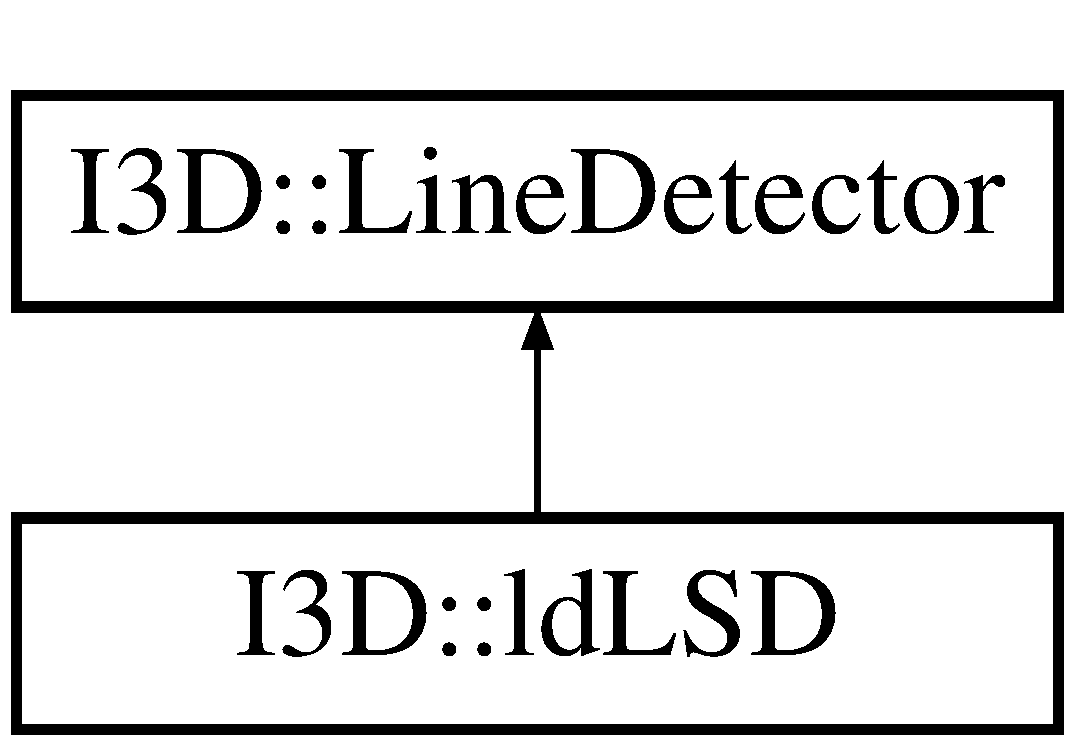
\includegraphics[height=2.000000cm]{class_i3_d_1_1ld_l_s_d}
\end{center}
\end{figure}
\subsection*{Métodos públicos}
\begin{DoxyCompactItemize}
\item 
\hyperlink{class_i3_d_1_1ld_l_s_d_a3f2eba9f10daaeab35a1adc7f628c11a}{ld\+L\+SD} (const cv\+::\+Scalar \&angletol=cv\+::\+Scalar(0, C\+V\+\_\+\+PI/2))
\begin{DoxyCompactList}\small\item\em Constructora de la clase \hyperlink{class_i3_d_1_1ld_l_s_d}{ld\+L\+SD}. \end{DoxyCompactList}\item 
\hyperlink{class_i3_d_1_1ld_l_s_d_aea5de322f9c8a8f6ab09ff477e9ab340}{$\sim$ld\+L\+SD} ()
\begin{DoxyCompactList}\small\item\em Destructora de la clase \hyperlink{class_i3_d_1_1ld_l_s_d}{ld\+L\+SD}. \end{DoxyCompactList}\item 
int \hyperlink{class_i3_d_1_1ld_l_s_d_a451a9385fb8abf87d6c462321518c439}{run} (cv\+::\+Mat \&image) override
\begin{DoxyCompactList}\small\item\em Ejecuta el detector de lineas L\+SD. \end{DoxyCompactList}\item 
int \hyperlink{class_i3_d_1_1ld_l_s_d_ab688b28c6cd6e0915404baf9329415d8}{run} (cv\+::\+Mat \&image, const cv\+::\+Scalar \&angletol) override
\begin{DoxyCompactList}\small\item\em Ejecuta el detector de lineas L\+SD. \end{DoxyCompactList}\end{DoxyCompactItemize}
\subsection*{Otros miembros heredados}


\subsection{Descripción detallada}
Clase para la detección de lineas mediante Line \hyperlink{class_i3_d_1_1_segment}{Segment} Detector. 

\subsection{Documentación del constructor y destructor}
\index{I3\+D\+::ld\+L\+SD@{I3\+D\+::ld\+L\+SD}!ld\+L\+SD@{ld\+L\+SD}}
\index{ld\+L\+SD@{ld\+L\+SD}!I3\+D\+::ld\+L\+SD@{I3\+D\+::ld\+L\+SD}}
\subsubsection[{\texorpdfstring{ld\+L\+S\+D(const cv\+::\+Scalar \&angletol=cv\+::\+Scalar(0, C\+V\+\_\+\+P\+I/2))}{ldLSD(const cv::Scalar &angletol=cv::Scalar(0, CV_PI/2))}}]{\setlength{\rightskip}{0pt plus 5cm}I3\+D\+::ld\+L\+S\+D\+::ld\+L\+SD (
\begin{DoxyParamCaption}
\item[{const cv\+::\+Scalar \&}]{angletol = {\ttfamily cv\+:\+:Scalar(0,~CV\+\_\+PI~/~2)}}
\end{DoxyParamCaption}
)\hspace{0.3cm}{\ttfamily [inline]}}\hypertarget{class_i3_d_1_1ld_l_s_d_a3f2eba9f10daaeab35a1adc7f628c11a}{}\label{class_i3_d_1_1ld_l_s_d_a3f2eba9f10daaeab35a1adc7f628c11a}


Constructora de la clase \hyperlink{class_i3_d_1_1ld_l_s_d}{ld\+L\+SD}. 


\begin{DoxyParams}[1]{Parámetros}
\mbox{\tt in}  & {\em angletol} & Angulo y tolerancia \\
\hline
\end{DoxyParams}
\index{I3\+D\+::ld\+L\+SD@{I3\+D\+::ld\+L\+SD}!````~ld\+L\+SD@{$\sim$ld\+L\+SD}}
\index{````~ld\+L\+SD@{$\sim$ld\+L\+SD}!I3\+D\+::ld\+L\+SD@{I3\+D\+::ld\+L\+SD}}
\subsubsection[{\texorpdfstring{$\sim$ld\+L\+S\+D()}{~ldLSD()}}]{\setlength{\rightskip}{0pt plus 5cm}I3\+D\+::ld\+L\+S\+D\+::$\sim$ld\+L\+SD (
\begin{DoxyParamCaption}
{}
\end{DoxyParamCaption}
)\hspace{0.3cm}{\ttfamily [inline]}}\hypertarget{class_i3_d_1_1ld_l_s_d_aea5de322f9c8a8f6ab09ff477e9ab340}{}\label{class_i3_d_1_1ld_l_s_d_aea5de322f9c8a8f6ab09ff477e9ab340}


Destructora de la clase \hyperlink{class_i3_d_1_1ld_l_s_d}{ld\+L\+SD}. 



\subsection{Documentación de las funciones miembro}
\index{I3\+D\+::ld\+L\+SD@{I3\+D\+::ld\+L\+SD}!run@{run}}
\index{run@{run}!I3\+D\+::ld\+L\+SD@{I3\+D\+::ld\+L\+SD}}
\subsubsection[{\texorpdfstring{run(cv\+::\+Mat \&image) override}{run(cv::Mat &image) override}}]{\setlength{\rightskip}{0pt plus 5cm}int I3\+D\+::ld\+L\+S\+D\+::run (
\begin{DoxyParamCaption}
\item[{cv\+::\+Mat \&}]{image}
\end{DoxyParamCaption}
)\hspace{0.3cm}{\ttfamily [override]}, {\ttfamily [virtual]}}\hypertarget{class_i3_d_1_1ld_l_s_d_a451a9385fb8abf87d6c462321518c439}{}\label{class_i3_d_1_1ld_l_s_d_a451a9385fb8abf87d6c462321518c439}


Ejecuta el detector de lineas L\+SD. 


\begin{DoxyParams}[1]{Parámetros}
\mbox{\tt in}  & {\em image} & Imagen en la cual se quieren detectar las lineas. \\
\hline
\end{DoxyParams}
\begin{DoxyReturn}{Devuelve}
Error 
\end{DoxyReturn}


Implementa \hyperlink{class_i3_d_1_1_line_detector_ad439cb59972938259f6b36bcdbb644b7}{I3\+D\+::\+Line\+Detector}.

\index{I3\+D\+::ld\+L\+SD@{I3\+D\+::ld\+L\+SD}!run@{run}}
\index{run@{run}!I3\+D\+::ld\+L\+SD@{I3\+D\+::ld\+L\+SD}}
\subsubsection[{\texorpdfstring{run(cv\+::\+Mat \&image, const cv\+::\+Scalar \&angletol) override}{run(cv::Mat &image, const cv::Scalar &angletol) override}}]{\setlength{\rightskip}{0pt plus 5cm}int I3\+D\+::ld\+L\+S\+D\+::run (
\begin{DoxyParamCaption}
\item[{cv\+::\+Mat \&}]{image, }
\item[{const cv\+::\+Scalar \&}]{angletol}
\end{DoxyParamCaption}
)\hspace{0.3cm}{\ttfamily [override]}, {\ttfamily [virtual]}}\hypertarget{class_i3_d_1_1ld_l_s_d_ab688b28c6cd6e0915404baf9329415d8}{}\label{class_i3_d_1_1ld_l_s_d_ab688b28c6cd6e0915404baf9329415d8}


Ejecuta el detector de lineas L\+SD. 


\begin{DoxyParams}[1]{Parámetros}
\mbox{\tt in}  & {\em image} & Imagen en la cual se quieren detectar las lineas. \\
\hline
\mbox{\tt in}  & {\em angletol} & Angulo y tolerancia \\
\hline
\end{DoxyParams}
\begin{DoxyReturn}{Devuelve}
Error 
\end{DoxyReturn}


Implementa \hyperlink{class_i3_d_1_1_line_detector_abc00c6e15e2386a32720886d60a20ccd}{I3\+D\+::\+Line\+Detector}.



La documentación para esta clase fue generada a partir de los siguientes ficheros\+:\begin{DoxyCompactItemize}
\item 
D\+:/\+Desarrollo/tidop/src/\hyperlink{_line_detector_8h}{Line\+Detector.\+h}\item 
D\+:/\+Desarrollo/tidop/src/\hyperlink{linedetector_8cpp}{linedetector.\+cpp}\end{DoxyCompactItemize}

\hypertarget{class_i3_d_1_1ld_l_s_w_m_s}{}\section{Referencia de la Clase I3D\+:\+:ld\+L\+S\+W\+MS}
\label{class_i3_d_1_1ld_l_s_w_m_s}\index{I3\+D\+::ld\+L\+S\+W\+MS@{I3\+D\+::ld\+L\+S\+W\+MS}}


Clase para la detección de lineas mediante L\+S\+W\+MS.  




{\ttfamily \#include $<$Line\+Detector.\+h$>$}

Diagrama de herencias de I3D\+:\+:ld\+L\+S\+W\+MS\begin{figure}[H]
\begin{center}
\leavevmode
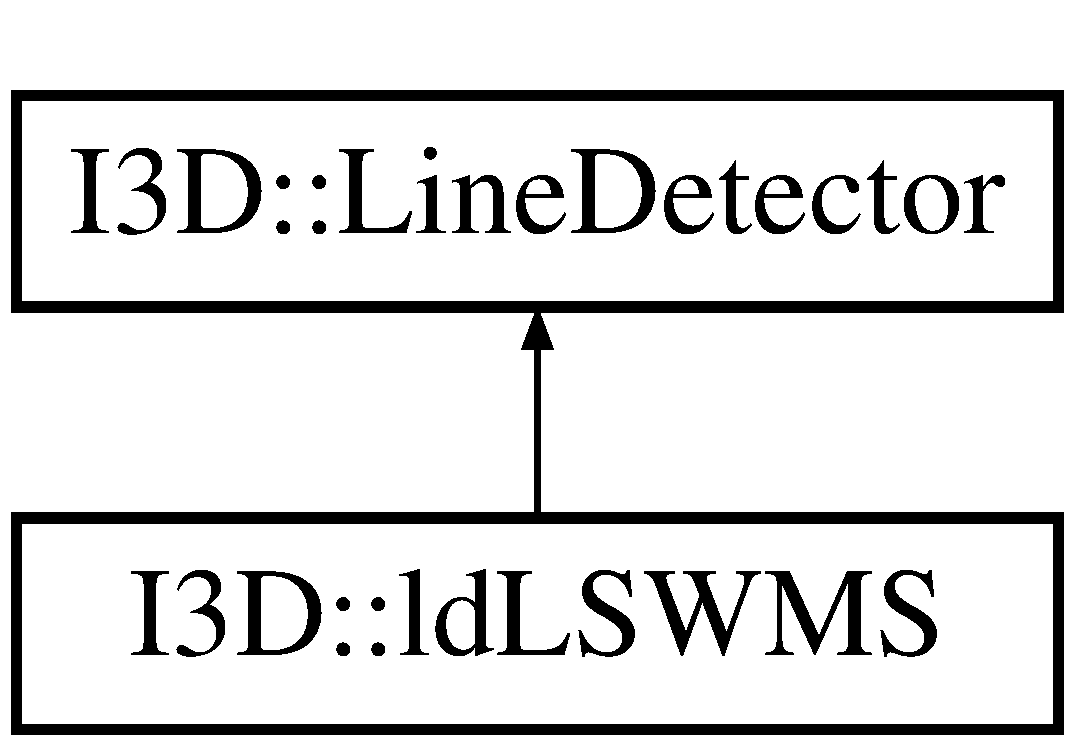
\includegraphics[height=2.000000cm]{class_i3_d_1_1ld_l_s_w_m_s}
\end{center}
\end{figure}
\subsection*{Métodos públicos}
\begin{DoxyCompactItemize}
\item 
\hyperlink{class_i3_d_1_1ld_l_s_w_m_s_a3de74908a087b8e6b0525a2f6c943568}{ld\+L\+S\+W\+MS} (cv\+::\+Size size, cv\+::\+Scalar \+\_\+angletol=cv\+::\+Scalar(0, C\+V\+\_\+\+PI/2))
\begin{DoxyCompactList}\small\item\em Constructora de la clase \hyperlink{class_i3_d_1_1ld_l_s_w_m_s}{ld\+L\+S\+W\+MS}. \end{DoxyCompactList}\item 
\hyperlink{class_i3_d_1_1ld_l_s_w_m_s_a0d98071e0e8b797670a79bfd77e8d6d5}{$\sim$ld\+L\+S\+W\+MS} ()
\begin{DoxyCompactList}\small\item\em Destructora de la clase \hyperlink{class_i3_d_1_1ld_l_s_w_m_s}{ld\+L\+S\+W\+MS}. \end{DoxyCompactList}\item 
void \hyperlink{class_i3_d_1_1ld_l_s_w_m_s_afe64627e711a33cf37bd4d8b2430c3a1}{draw\+Lines} (cv\+::\+Mat \&canvas, cv\+::\+Scalar color=cv\+::\+Scalar(0, 255, 0), int thickness=1, int line\+Type=cv\+::\+L\+I\+N\+E\+\_\+8)
\begin{DoxyCompactList}\small\item\em Dibujo de lineas. \end{DoxyCompactList}\item 
void \hyperlink{class_i3_d_1_1ld_l_s_w_m_s_ab32e51dd8ef06da0f707ec2a51919660}{run} (cv\+::\+Mat \&image) override
\begin{DoxyCompactList}\small\item\em Ejecuta el detector de lineas L\+S\+W\+MS. \end{DoxyCompactList}\end{DoxyCompactItemize}
\subsection*{Otros miembros heredados}


\subsection{Descripción detallada}
Clase para la detección de lineas mediante L\+S\+W\+MS. 

Line \hyperlink{class_i3_d_1_1_segment}{Segment} detection using Weighted Mean-\/\+Shift 

\subsection{Documentación del constructor y destructor}
\index{I3\+D\+::ld\+L\+S\+W\+MS@{I3\+D\+::ld\+L\+S\+W\+MS}!ld\+L\+S\+W\+MS@{ld\+L\+S\+W\+MS}}
\index{ld\+L\+S\+W\+MS@{ld\+L\+S\+W\+MS}!I3\+D\+::ld\+L\+S\+W\+MS@{I3\+D\+::ld\+L\+S\+W\+MS}}
\subsubsection[{\texorpdfstring{ld\+L\+S\+W\+M\+S(cv\+::\+Size size, cv\+::\+Scalar \+\_\+angletol=cv\+::\+Scalar(0, C\+V\+\_\+\+P\+I/2))}{ldLSWMS(cv::Size size, cv::Scalar _angletol=cv::Scalar(0, CV_PI/2))}}]{\setlength{\rightskip}{0pt plus 5cm}I3\+D\+::ld\+L\+S\+W\+M\+S\+::ld\+L\+S\+W\+MS (
\begin{DoxyParamCaption}
\item[{cv\+::\+Size}]{size, }
\item[{cv\+::\+Scalar}]{\+\_\+angletol = {\ttfamily cv\+:\+:Scalar(0,~CV\+\_\+PI~/~2)}}
\end{DoxyParamCaption}
)}\hypertarget{class_i3_d_1_1ld_l_s_w_m_s_a3de74908a087b8e6b0525a2f6c943568}{}\label{class_i3_d_1_1ld_l_s_w_m_s_a3de74908a087b8e6b0525a2f6c943568}


Constructora de la clase \hyperlink{class_i3_d_1_1ld_l_s_w_m_s}{ld\+L\+S\+W\+MS}. 


\begin{DoxyParams}{Parámetros}
{\em size} & \\
\hline
{\em \+\_\+angletol} & Angulo y tolerancia \\
\hline
\end{DoxyParams}
\index{I3\+D\+::ld\+L\+S\+W\+MS@{I3\+D\+::ld\+L\+S\+W\+MS}!````~ld\+L\+S\+W\+MS@{$\sim$ld\+L\+S\+W\+MS}}
\index{````~ld\+L\+S\+W\+MS@{$\sim$ld\+L\+S\+W\+MS}!I3\+D\+::ld\+L\+S\+W\+MS@{I3\+D\+::ld\+L\+S\+W\+MS}}
\subsubsection[{\texorpdfstring{$\sim$ld\+L\+S\+W\+M\+S()}{~ldLSWMS()}}]{\setlength{\rightskip}{0pt plus 5cm}I3\+D\+::ld\+L\+S\+W\+M\+S\+::$\sim$ld\+L\+S\+W\+MS (
\begin{DoxyParamCaption}
{}
\end{DoxyParamCaption}
)}\hypertarget{class_i3_d_1_1ld_l_s_w_m_s_a0d98071e0e8b797670a79bfd77e8d6d5}{}\label{class_i3_d_1_1ld_l_s_w_m_s_a0d98071e0e8b797670a79bfd77e8d6d5}


Destructora de la clase \hyperlink{class_i3_d_1_1ld_l_s_w_m_s}{ld\+L\+S\+W\+MS}. 



\subsection{Documentación de las funciones miembro}
\index{I3\+D\+::ld\+L\+S\+W\+MS@{I3\+D\+::ld\+L\+S\+W\+MS}!draw\+Lines@{draw\+Lines}}
\index{draw\+Lines@{draw\+Lines}!I3\+D\+::ld\+L\+S\+W\+MS@{I3\+D\+::ld\+L\+S\+W\+MS}}
\subsubsection[{\texorpdfstring{draw\+Lines(cv\+::\+Mat \&canvas, cv\+::\+Scalar color=cv\+::\+Scalar(0, 255, 0), int thickness=1, int line\+Type=cv\+::\+L\+I\+N\+E\+\_\+8)}{drawLines(cv::Mat &canvas, cv::Scalar color=cv::Scalar(0, 255, 0), int thickness=1, int lineType=cv::LINE_8)}}]{\setlength{\rightskip}{0pt plus 5cm}void I3\+D\+::ld\+L\+S\+W\+M\+S\+::draw\+Lines (
\begin{DoxyParamCaption}
\item[{cv\+::\+Mat \&}]{canvas, }
\item[{cv\+::\+Scalar}]{color = {\ttfamily cv\+:\+:Scalar(0,~255,~0)}, }
\item[{int}]{thickness = {\ttfamily 1}, }
\item[{int}]{line\+Type = {\ttfamily cv\+:\+:LINE\+\_\+8}}
\end{DoxyParamCaption}
)}\hypertarget{class_i3_d_1_1ld_l_s_w_m_s_afe64627e711a33cf37bd4d8b2430c3a1}{}\label{class_i3_d_1_1ld_l_s_w_m_s_afe64627e711a33cf37bd4d8b2430c3a1}


Dibujo de lineas. 

Dibuja las lineas obtenidas mediante L\+S\+W\+MS


\begin{DoxyParams}{Parámetros}
{\em canvas} & cv\+::\+Mat donde se van a pintar las lineas. \\
\hline
{\em color} & Color de las lineas \\
\hline
{\em thickness} & Grosor de las lineas \\
\hline
{\em line\+Type} & Tipo de linea \\
\hline
\end{DoxyParams}
\index{I3\+D\+::ld\+L\+S\+W\+MS@{I3\+D\+::ld\+L\+S\+W\+MS}!run@{run}}
\index{run@{run}!I3\+D\+::ld\+L\+S\+W\+MS@{I3\+D\+::ld\+L\+S\+W\+MS}}
\subsubsection[{\texorpdfstring{run(cv\+::\+Mat \&image) override}{run(cv::Mat &image) override}}]{\setlength{\rightskip}{0pt plus 5cm}void I3\+D\+::ld\+L\+S\+W\+M\+S\+::run (
\begin{DoxyParamCaption}
\item[{cv\+::\+Mat \&}]{image}
\end{DoxyParamCaption}
)\hspace{0.3cm}{\ttfamily [override]}, {\ttfamily [virtual]}}\hypertarget{class_i3_d_1_1ld_l_s_w_m_s_ab32e51dd8ef06da0f707ec2a51919660}{}\label{class_i3_d_1_1ld_l_s_w_m_s_ab32e51dd8ef06da0f707ec2a51919660}


Ejecuta el detector de lineas L\+S\+W\+MS. 


\begin{DoxyParams}{Parámetros}
{\em image} & Imagen en la cual se quieren detectar las lineas. \\
\hline
\end{DoxyParams}


Implementa \hyperlink{class_i3_d_1_1_line_detector_ad439cb59972938259f6b36bcdbb644b7}{I3\+D\+::\+Line\+Detector}.



La documentación para esta clase fue generada a partir de los siguientes ficheros\+:\begin{DoxyCompactItemize}
\item 
D\+:/\+Desarrollo/tidop/src/\hyperlink{_line_detector_8h}{Line\+Detector.\+h}\item 
D\+:/\+Desarrollo/tidop/src/\hyperlink{linedetector_8cpp}{linedetector.\+cpp}\end{DoxyCompactItemize}

\hypertarget{class_i3_d_1_1_line_detector}{}\section{Referencia de la Clase I3D\+:\+:Line\+Detector}
\label{class_i3_d_1_1_line_detector}\index{I3\+D\+::\+Line\+Detector@{I3\+D\+::\+Line\+Detector}}


Clase base abstracta para los detectores de lineas.  




{\ttfamily \#include $<$Line\+Detector.\+h$>$}

Diagrama de herencias de I3D\+:\+:Line\+Detector\begin{figure}[H]
\begin{center}
\leavevmode
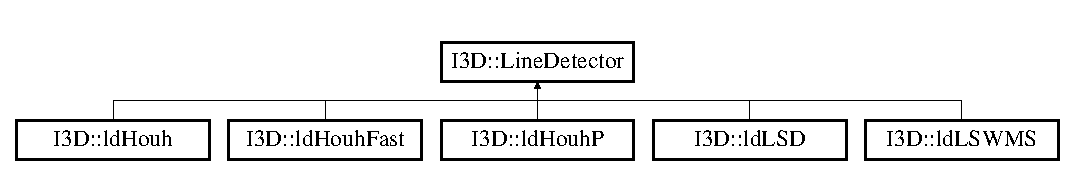
\includegraphics[height=2.000000cm]{class_i3_d_1_1_line_detector}
\end{center}
\end{figure}
\subsection*{Métodos públicos}
\begin{DoxyCompactItemize}
\item 
\hyperlink{class_i3_d_1_1_line_detector_a337305d13282d028b427787271e8d53d}{Line\+Detector} (\hyperlink{namespace_i3_d_ac3913218d62e4e56ed38931636256ae2}{L\+D\+\_\+\+T\+Y\+PE} type, const cv\+::\+Scalar \&angletol)
\begin{DoxyCompactList}\small\item\em Constructor. \end{DoxyCompactList}\item 
virtual \hyperlink{class_i3_d_1_1_line_detector_a1725fe70dfe60c340fb9c5f7609110e4}{$\sim$\+Line\+Detector} ()
\begin{DoxyCompactList}\small\item\em Destructora. \end{DoxyCompactList}\item 
void \hyperlink{class_i3_d_1_1_line_detector_a057a60f78b7bfa5b6f6f31d8ee8bfe87}{draw\+Lines} (cv\+::\+Mat \&canvas, const cv\+::\+Scalar \&color=cv\+::\+Scalar(0, 255, 0), int thickness=1, int line\+Type=cv\+::\+L\+I\+N\+E\+\_\+8) const 
\begin{DoxyCompactList}\small\item\em Dibujo de lineas. \end{DoxyCompactList}\item 
virtual int \hyperlink{class_i3_d_1_1_line_detector_ad439cb59972938259f6b36bcdbb644b7}{run} (cv\+::\+Mat \&image)=0
\begin{DoxyCompactList}\small\item\em Ejecuta el detector de lineas. \end{DoxyCompactList}\item 
virtual int \hyperlink{class_i3_d_1_1_line_detector_abc00c6e15e2386a32720886d60a20ccd}{run} (cv\+::\+Mat \&image, const cv\+::\+Scalar \&angletol)=0
\begin{DoxyCompactList}\small\item\em Ejecuta el detector de lineas. \end{DoxyCompactList}\item 
\hyperlink{namespace_i3_d_ac3913218d62e4e56ed38931636256ae2}{L\+D\+\_\+\+T\+Y\+PE} \hyperlink{class_i3_d_1_1_line_detector_a93add9094451f5b622c85821f29b70f9}{get\+Type} () const 
\begin{DoxyCompactList}\small\item\em Establece rango angular en el cual se buscarán las líneas. \end{DoxyCompactList}\item 
const std\+::vector$<$ \hyperlink{group___geometric_entities_ga483b43891a1b33d99406fdc397e9a445}{Line} $>$ \& \hyperlink{class_i3_d_1_1_line_detector_a289e75fcd682e07fc748ddc096e98349}{get\+Lines} () const 
\begin{DoxyCompactList}\small\item\em Devuelve una referencia a las líneas detectadas. \end{DoxyCompactList}\end{DoxyCompactItemize}
\subsection*{Métodos protegidos}
\begin{DoxyCompactItemize}
\item 
void \hyperlink{class_i3_d_1_1_line_detector_a3021a94cd1cb6d53f855844eab5188a9}{set\+Angle\+Range} (const cv\+::\+Scalar \&at)
\begin{DoxyCompactList}\small\item\em Establece rango angular en el cual se buscarán las líneas. \end{DoxyCompactList}\end{DoxyCompactItemize}
\subsection*{Atributos protegidos}
\begin{DoxyCompactItemize}
\item 
\hyperlink{namespace_i3_d_ac3913218d62e4e56ed38931636256ae2}{L\+D\+\_\+\+T\+Y\+PE} \hyperlink{class_i3_d_1_1_line_detector_ae988a8bc160374b7314ccff2495deced}{m\+Type}
\begin{DoxyCompactList}\small\item\em Tipo de detector de linea. \end{DoxyCompactList}\item 
double \hyperlink{class_i3_d_1_1_line_detector_a3d359c9077a01c74308c4c05975a17d5}{m\+Min\+Theta}
\begin{DoxyCompactList}\small\item\em Angulo mínimo. \end{DoxyCompactList}\item 
double \hyperlink{class_i3_d_1_1_line_detector_afbb629bc06fdc61296e03b93506e0c37}{m\+Max\+Theta}
\begin{DoxyCompactList}\small\item\em Angulo máximo. \end{DoxyCompactList}\item 
std\+::vector$<$ \hyperlink{group___geometric_entities_ga483b43891a1b33d99406fdc397e9a445}{Line} $>$ \hyperlink{class_i3_d_1_1_line_detector_aa5a297aa79f93e96dcb4574bc051f3d4}{m\+Lines}
\begin{DoxyCompactList}\small\item\em Lineas detectadas. \end{DoxyCompactList}\end{DoxyCompactItemize}


\subsection{Descripción detallada}
Clase base abstracta para los detectores de lineas. 

Contiene la declaración de los métodos que deben definir las clases que hereden de ella. 

\subsection{Documentación del constructor y destructor}
\index{I3\+D\+::\+Line\+Detector@{I3\+D\+::\+Line\+Detector}!Line\+Detector@{Line\+Detector}}
\index{Line\+Detector@{Line\+Detector}!I3\+D\+::\+Line\+Detector@{I3\+D\+::\+Line\+Detector}}
\subsubsection[{\texorpdfstring{Line\+Detector(\+L\+D\+\_\+\+T\+Y\+P\+E type, const cv\+::\+Scalar \&angletol)}{LineDetector(LD_TYPE type, const cv::Scalar &angletol)}}]{\setlength{\rightskip}{0pt plus 5cm}I3\+D\+::\+Line\+Detector\+::\+Line\+Detector (
\begin{DoxyParamCaption}
\item[{{\bf L\+D\+\_\+\+T\+Y\+PE}}]{type, }
\item[{const cv\+::\+Scalar \&}]{angletol}
\end{DoxyParamCaption}
)\hspace{0.3cm}{\ttfamily [inline]}}\hypertarget{class_i3_d_1_1_line_detector_a337305d13282d028b427787271e8d53d}{}\label{class_i3_d_1_1_line_detector_a337305d13282d028b427787271e8d53d}


Constructor. 

Constructora 
\begin{DoxyParams}[1]{Parámetros}
\mbox{\tt in}  & {\em type} & Tipo de detector de linea. \\
\hline
\mbox{\tt in}  & {\em angletol} & Angulo y tolerancia \\
\hline
\end{DoxyParams}
\index{I3\+D\+::\+Line\+Detector@{I3\+D\+::\+Line\+Detector}!````~Line\+Detector@{$\sim$\+Line\+Detector}}
\index{````~Line\+Detector@{$\sim$\+Line\+Detector}!I3\+D\+::\+Line\+Detector@{I3\+D\+::\+Line\+Detector}}
\subsubsection[{\texorpdfstring{$\sim$\+Line\+Detector()}{~LineDetector()}}]{\setlength{\rightskip}{0pt plus 5cm}virtual I3\+D\+::\+Line\+Detector\+::$\sim$\+Line\+Detector (
\begin{DoxyParamCaption}
{}
\end{DoxyParamCaption}
)\hspace{0.3cm}{\ttfamily [inline]}, {\ttfamily [virtual]}}\hypertarget{class_i3_d_1_1_line_detector_a1725fe70dfe60c340fb9c5f7609110e4}{}\label{class_i3_d_1_1_line_detector_a1725fe70dfe60c340fb9c5f7609110e4}


Destructora. 



\subsection{Documentación de las funciones miembro}
\index{I3\+D\+::\+Line\+Detector@{I3\+D\+::\+Line\+Detector}!draw\+Lines@{draw\+Lines}}
\index{draw\+Lines@{draw\+Lines}!I3\+D\+::\+Line\+Detector@{I3\+D\+::\+Line\+Detector}}
\subsubsection[{\texorpdfstring{draw\+Lines(cv\+::\+Mat \&canvas, const cv\+::\+Scalar \&color=cv\+::\+Scalar(0, 255, 0), int thickness=1, int line\+Type=cv\+::\+L\+I\+N\+E\+\_\+8) const }{drawLines(cv::Mat &canvas, const cv::Scalar &color=cv::Scalar(0, 255, 0), int thickness=1, int lineType=cv::LINE_8) const }}]{\setlength{\rightskip}{0pt plus 5cm}void I3\+D\+::\+Line\+Detector\+::draw\+Lines (
\begin{DoxyParamCaption}
\item[{cv\+::\+Mat \&}]{canvas, }
\item[{const cv\+::\+Scalar \&}]{color = {\ttfamily cv\+:\+:Scalar(0,~255,~0)}, }
\item[{int}]{thickness = {\ttfamily 1}, }
\item[{int}]{line\+Type = {\ttfamily cv\+:\+:LINE\+\_\+8}}
\end{DoxyParamCaption}
) const}\hypertarget{class_i3_d_1_1_line_detector_a057a60f78b7bfa5b6f6f31d8ee8bfe87}{}\label{class_i3_d_1_1_line_detector_a057a60f78b7bfa5b6f6f31d8ee8bfe87}


Dibujo de lineas. 

Dibuja las lineas obtenidas con el metodo de detección de lineas empleado


\begin{DoxyParams}[1]{Parámetros}
\mbox{\tt in}  & {\em canvas} & cv\+::\+Mat donde se van a pintar las lineas. \\
\hline
\mbox{\tt in}  & {\em color} & Color de las lineas \\
\hline
\mbox{\tt in}  & {\em thickness} & Grosor de las lineas \\
\hline
\mbox{\tt in}  & {\em line\+Type} & Tipo de linea \\
\hline
\end{DoxyParams}
\index{I3\+D\+::\+Line\+Detector@{I3\+D\+::\+Line\+Detector}!get\+Lines@{get\+Lines}}
\index{get\+Lines@{get\+Lines}!I3\+D\+::\+Line\+Detector@{I3\+D\+::\+Line\+Detector}}
\subsubsection[{\texorpdfstring{get\+Lines() const }{getLines() const }}]{\setlength{\rightskip}{0pt plus 5cm}const std\+::vector$<${\bf Line}$>$\& I3\+D\+::\+Line\+Detector\+::get\+Lines (
\begin{DoxyParamCaption}
{}
\end{DoxyParamCaption}
) const\hspace{0.3cm}{\ttfamily [inline]}}\hypertarget{class_i3_d_1_1_line_detector_a289e75fcd682e07fc748ddc096e98349}{}\label{class_i3_d_1_1_line_detector_a289e75fcd682e07fc748ddc096e98349}


Devuelve una referencia a las líneas detectadas. 

\begin{DoxyReturn}{Devuelve}
Lineas 
\end{DoxyReturn}
\index{I3\+D\+::\+Line\+Detector@{I3\+D\+::\+Line\+Detector}!get\+Type@{get\+Type}}
\index{get\+Type@{get\+Type}!I3\+D\+::\+Line\+Detector@{I3\+D\+::\+Line\+Detector}}
\subsubsection[{\texorpdfstring{get\+Type() const }{getType() const }}]{\setlength{\rightskip}{0pt plus 5cm}{\bf L\+D\+\_\+\+T\+Y\+PE} I3\+D\+::\+Line\+Detector\+::get\+Type (
\begin{DoxyParamCaption}
{}
\end{DoxyParamCaption}
) const\hspace{0.3cm}{\ttfamily [inline]}}\hypertarget{class_i3_d_1_1_line_detector_a93add9094451f5b622c85821f29b70f9}{}\label{class_i3_d_1_1_line_detector_a93add9094451f5b622c85821f29b70f9}


Establece rango angular en el cual se buscarán las líneas. 

\begin{DoxyReturn}{Devuelve}

\end{DoxyReturn}
\index{I3\+D\+::\+Line\+Detector@{I3\+D\+::\+Line\+Detector}!run@{run}}
\index{run@{run}!I3\+D\+::\+Line\+Detector@{I3\+D\+::\+Line\+Detector}}
\subsubsection[{\texorpdfstring{run(cv\+::\+Mat \&image)=0}{run(cv::Mat &image)=0}}]{\setlength{\rightskip}{0pt plus 5cm}virtual int I3\+D\+::\+Line\+Detector\+::run (
\begin{DoxyParamCaption}
\item[{cv\+::\+Mat \&}]{image}
\end{DoxyParamCaption}
)\hspace{0.3cm}{\ttfamily [pure virtual]}}\hypertarget{class_i3_d_1_1_line_detector_ad439cb59972938259f6b36bcdbb644b7}{}\label{class_i3_d_1_1_line_detector_ad439cb59972938259f6b36bcdbb644b7}


Ejecuta el detector de lineas. 


\begin{DoxyParams}[1]{Parámetros}
\mbox{\tt in}  & {\em image} & Imagen en la cual se quieren detectar las lineas. \\
\hline
\end{DoxyParams}
\begin{DoxyReturn}{Devuelve}
Error 
\end{DoxyReturn}


Implementado en \hyperlink{class_i3_d_1_1ld_l_s_d_a451a9385fb8abf87d6c462321518c439}{I3\+D\+::ld\+L\+SD}, \hyperlink{class_i3_d_1_1ld_houh_fast_a9cbcde2e4327ba3fd7c65d404bea5ee7}{I3\+D\+::ld\+Houh\+Fast}, \hyperlink{class_i3_d_1_1ld_houh_p_a91b42a50eb80dfcb9f5cf1bdf0d8c908}{I3\+D\+::ld\+HouhP} y \hyperlink{class_i3_d_1_1ld_houh_a17c6836029eeb9448e6bd661c1aac16c}{I3\+D\+::ld\+Houh}.

\index{I3\+D\+::\+Line\+Detector@{I3\+D\+::\+Line\+Detector}!run@{run}}
\index{run@{run}!I3\+D\+::\+Line\+Detector@{I3\+D\+::\+Line\+Detector}}
\subsubsection[{\texorpdfstring{run(cv\+::\+Mat \&image, const cv\+::\+Scalar \&angletol)=0}{run(cv::Mat &image, const cv::Scalar &angletol)=0}}]{\setlength{\rightskip}{0pt plus 5cm}virtual int I3\+D\+::\+Line\+Detector\+::run (
\begin{DoxyParamCaption}
\item[{cv\+::\+Mat \&}]{image, }
\item[{const cv\+::\+Scalar \&}]{angletol}
\end{DoxyParamCaption}
)\hspace{0.3cm}{\ttfamily [pure virtual]}}\hypertarget{class_i3_d_1_1_line_detector_abc00c6e15e2386a32720886d60a20ccd}{}\label{class_i3_d_1_1_line_detector_abc00c6e15e2386a32720886d60a20ccd}


Ejecuta el detector de lineas. 


\begin{DoxyParams}[1]{Parámetros}
\mbox{\tt in}  & {\em image} & Imagen en la cual se quieren detectar las lineas. \\
\hline
\mbox{\tt in}  & {\em angletol} & Angulo y tolerancia \\
\hline
\end{DoxyParams}
\begin{DoxyReturn}{Devuelve}
Error 
\end{DoxyReturn}


Implementado en \hyperlink{class_i3_d_1_1ld_l_s_d_ab688b28c6cd6e0915404baf9329415d8}{I3\+D\+::ld\+L\+SD}, \hyperlink{class_i3_d_1_1ld_houh_fast_a41fd58bdeeb31893f4a98a90ce9ec516}{I3\+D\+::ld\+Houh\+Fast}, \hyperlink{class_i3_d_1_1ld_houh_p_ad00dcfc80128ea426b2fff2878c7e723}{I3\+D\+::ld\+HouhP} y \hyperlink{class_i3_d_1_1ld_houh_a548494c74a114c679ddc050dc9fd991a}{I3\+D\+::ld\+Houh}.

\index{I3\+D\+::\+Line\+Detector@{I3\+D\+::\+Line\+Detector}!set\+Angle\+Range@{set\+Angle\+Range}}
\index{set\+Angle\+Range@{set\+Angle\+Range}!I3\+D\+::\+Line\+Detector@{I3\+D\+::\+Line\+Detector}}
\subsubsection[{\texorpdfstring{set\+Angle\+Range(const cv\+::\+Scalar \&at)}{setAngleRange(const cv::Scalar &at)}}]{\setlength{\rightskip}{0pt plus 5cm}void I3\+D\+::\+Line\+Detector\+::set\+Angle\+Range (
\begin{DoxyParamCaption}
\item[{const cv\+::\+Scalar \&}]{at}
\end{DoxyParamCaption}
)\hspace{0.3cm}{\ttfamily [protected]}}\hypertarget{class_i3_d_1_1_line_detector_a3021a94cd1cb6d53f855844eab5188a9}{}\label{class_i3_d_1_1_line_detector_a3021a94cd1cb6d53f855844eab5188a9}


Establece rango angular en el cual se buscarán las líneas. 


\begin{DoxyParams}[1]{Parámetros}
\mbox{\tt in}  & {\em at} & Angulo y tolerancia \\
\hline
\end{DoxyParams}


\subsection{Documentación de los datos miembro}
\index{I3\+D\+::\+Line\+Detector@{I3\+D\+::\+Line\+Detector}!m\+Lines@{m\+Lines}}
\index{m\+Lines@{m\+Lines}!I3\+D\+::\+Line\+Detector@{I3\+D\+::\+Line\+Detector}}
\subsubsection[{\texorpdfstring{m\+Lines}{mLines}}]{\setlength{\rightskip}{0pt plus 5cm}std\+::vector$<${\bf Line}$>$ I3\+D\+::\+Line\+Detector\+::m\+Lines\hspace{0.3cm}{\ttfamily [protected]}}\hypertarget{class_i3_d_1_1_line_detector_aa5a297aa79f93e96dcb4574bc051f3d4}{}\label{class_i3_d_1_1_line_detector_aa5a297aa79f93e96dcb4574bc051f3d4}


Lineas detectadas. 

\index{I3\+D\+::\+Line\+Detector@{I3\+D\+::\+Line\+Detector}!m\+Max\+Theta@{m\+Max\+Theta}}
\index{m\+Max\+Theta@{m\+Max\+Theta}!I3\+D\+::\+Line\+Detector@{I3\+D\+::\+Line\+Detector}}
\subsubsection[{\texorpdfstring{m\+Max\+Theta}{mMaxTheta}}]{\setlength{\rightskip}{0pt plus 5cm}double I3\+D\+::\+Line\+Detector\+::m\+Max\+Theta\hspace{0.3cm}{\ttfamily [protected]}}\hypertarget{class_i3_d_1_1_line_detector_afbb629bc06fdc61296e03b93506e0c37}{}\label{class_i3_d_1_1_line_detector_afbb629bc06fdc61296e03b93506e0c37}


Angulo máximo. 

Angulo máximo para buscar lineas. \index{I3\+D\+::\+Line\+Detector@{I3\+D\+::\+Line\+Detector}!m\+Min\+Theta@{m\+Min\+Theta}}
\index{m\+Min\+Theta@{m\+Min\+Theta}!I3\+D\+::\+Line\+Detector@{I3\+D\+::\+Line\+Detector}}
\subsubsection[{\texorpdfstring{m\+Min\+Theta}{mMinTheta}}]{\setlength{\rightskip}{0pt plus 5cm}double I3\+D\+::\+Line\+Detector\+::m\+Min\+Theta\hspace{0.3cm}{\ttfamily [protected]}}\hypertarget{class_i3_d_1_1_line_detector_a3d359c9077a01c74308c4c05975a17d5}{}\label{class_i3_d_1_1_line_detector_a3d359c9077a01c74308c4c05975a17d5}


Angulo mínimo. 

Angulo mínimo para buscar lineas. \index{I3\+D\+::\+Line\+Detector@{I3\+D\+::\+Line\+Detector}!m\+Type@{m\+Type}}
\index{m\+Type@{m\+Type}!I3\+D\+::\+Line\+Detector@{I3\+D\+::\+Line\+Detector}}
\subsubsection[{\texorpdfstring{m\+Type}{mType}}]{\setlength{\rightskip}{0pt plus 5cm}{\bf L\+D\+\_\+\+T\+Y\+PE} I3\+D\+::\+Line\+Detector\+::m\+Type\hspace{0.3cm}{\ttfamily [protected]}}\hypertarget{class_i3_d_1_1_line_detector_ae988a8bc160374b7314ccff2495deced}{}\label{class_i3_d_1_1_line_detector_ae988a8bc160374b7314ccff2495deced}


Tipo de detector de linea. 



La documentación para esta clase fue generada a partir de los siguientes ficheros\+:\begin{DoxyCompactItemize}
\item 
C\+:/\+Desarrollo/tidop/src/\hyperlink{_line_detector_8h}{Line\+Detector.\+h}\item 
C\+:/\+Desarrollo/tidop/src/\hyperlink{linedetector_8cpp}{linedetector.\+cpp}\end{DoxyCompactItemize}

\hypertarget{class_i3_d_1_1_log_msg}{}\section{Referencia de la Clase I3D\+:\+:Log\+Msg}
\label{class_i3_d_1_1_log_msg}\index{I3\+D\+::\+Log\+Msg@{I3\+D\+::\+Log\+Msg}}


Clase para gestión de ficheros log.  




{\ttfamily \#include $<$Logger.\+h$>$}

\subsection*{Métodos públicos}
\begin{DoxyCompactItemize}
\item 
\hyperlink{class_i3_d_1_1_log_msg_a5cb7a7b1765778874c2b87d2245463c6}{Log\+Msg} ()
\begin{DoxyCompactList}\small\item\em Constructora \hyperlink{class_i3_d_1_1_log_msg}{Log\+Msg}. \end{DoxyCompactList}\item 
\hyperlink{class_i3_d_1_1_log_msg_ac6d1edcbbc1806f42114374f23cacb8d}{Log\+Msg} (const char $\ast$filename, \hyperlink{namespace_i3_d_ae1af0f2e3b629610c45222809ff521f6}{Log\+Level} ll=\hyperlink{namespace_i3_d_ae1af0f2e3b629610c45222809ff521f6a4490aa3d29644e716440fada68f54032}{Log\+Level\+::\+L\+O\+G\+\_\+\+E\+R\+R\+OR})
\begin{DoxyCompactList}\small\item\em Constructora \hyperlink{class_i3_d_1_1_log_msg}{Log\+Msg}. \end{DoxyCompactList}\item 
\hyperlink{class_i3_d_1_1_log_msg_aa0811c5bd5866194a285bd8d066a4f4c}{$\sim$\+Log\+Msg} ()
\item 
\hyperlink{class_i3_d_1_1_log_msg_ab0af596a2b1485e5d84d6bb948e7e34b}{I3\+D\+\_\+\+D\+E\+P\+R\+E\+C\+A\+T\+ED} (\char`\"{}log\+Print\+Debug( \hyperlink{class_i3_d_1_1_log_msg_a5a1ceb27d9529de8eb9b3fc9377e178a}{msg}, ...) or \hyperlink{class_i3_d_1_1_message_a525f877a41a1e7493188b2b720d1d254}{Message\+::message}(\hyperlink{class_i3_d_1_1_log_msg_a5a1ceb27d9529de8eb9b3fc9377e178a}{msg}, \+\_\+\+\_\+\+V\+A\+\_\+\+A\+R\+G\+S\+\_\+\+\_\+).print( \hyperlink{namespace_i3_d_a1c1740d2076e09b1a37b82e45a0327b5a918e87a1f80863c7ee35bfa2c58cc41e}{Message\+Level\+::\+M\+S\+G\+\_\+\+D\+E\+B\+UG}, \hyperlink{namespace_i3_d_a2ccb65ac6e08844c1175a235107fa103ace1cd665ada8b4f22dfa5f764fed6c6c}{Message\+Output\+::\+M\+S\+G\+\_\+\+C\+O\+N\+S\+O\+LE})\char`\"{}) static void debug\+Msg(const char $\ast$\hyperlink{class_i3_d_1_1_log_msg_a5a1ceb27d9529de8eb9b3fc9377e178a}{msg}
\begin{DoxyCompactList}\small\item\em Mensaje de depuración. \end{DoxyCompactList}\item 
\hyperlink{class_i3_d_1_1_log_msg_a17cce8fb482ad6bcfc0f3accd5d1a33b}{I3\+D\+\_\+\+D\+E\+P\+R\+E\+C\+A\+T\+ED} (\char`\"{}log\+Print\+Debug( \hyperlink{class_i3_d_1_1_log_msg_a5a1ceb27d9529de8eb9b3fc9377e178a}{msg}, ...) or \hyperlink{class_i3_d_1_1_message_a525f877a41a1e7493188b2b720d1d254}{Message\+::message}(\hyperlink{class_i3_d_1_1_log_msg_a5a1ceb27d9529de8eb9b3fc9377e178a}{msg}, \+\_\+\+\_\+\+V\+A\+\_\+\+A\+R\+G\+S\+\_\+\+\_\+).print( \hyperlink{namespace_i3_d_a1c1740d2076e09b1a37b82e45a0327b5a918e87a1f80863c7ee35bfa2c58cc41e}{Message\+Level\+::\+M\+S\+G\+\_\+\+D\+E\+B\+UG}, \hyperlink{namespace_i3_d_a2ccb65ac6e08844c1175a235107fa103a8c1a4761ebfadb227927517230ff7b02}{Message\+Output\+::\+M\+S\+G\+\_\+\+L\+OG}, \+\_\+\+\_\+\+F\+I\+L\+E\+\_\+\+\_\+, \+\_\+\+\_\+\+L\+I\+N\+E\+\_\+\+\_\+, I3\+D\+\_\+\+F\+U\+N\+C\+T\+I\+ON)\char`\"{}) static void debug\+Msg(const char $\ast$\hyperlink{class_i3_d_1_1_log_msg_ab59f20d39ef112d2196371ae0636d77c}{file}
\begin{DoxyCompactList}\small\item\em Debug\+Msg. \end{DoxyCompactList}\item 
int const char char \hyperlink{class_i3_d_1_1_log_msg_a4bb9bcc06243caa8745dd7e4dda702e0}{I3\+D\+\_\+\+D\+E\+P\+R\+E\+C\+A\+T\+ED} (\char`\"{}log\+Print\+Debug( \hyperlink{class_i3_d_1_1_log_msg_a5a1ceb27d9529de8eb9b3fc9377e178a}{msg}, ...) or \hyperlink{class_i3_d_1_1_message_a525f877a41a1e7493188b2b720d1d254}{Message\+::message}(\hyperlink{class_i3_d_1_1_log_msg_a5a1ceb27d9529de8eb9b3fc9377e178a}{msg}, \+\_\+\+\_\+\+V\+A\+\_\+\+A\+R\+G\+S\+\_\+\+\_\+).print( \hyperlink{namespace_i3_d_a1c1740d2076e09b1a37b82e45a0327b5a918e87a1f80863c7ee35bfa2c58cc41e}{Message\+Level\+::\+M\+S\+G\+\_\+\+D\+E\+B\+UG}, \hyperlink{namespace_i3_d_a2ccb65ac6e08844c1175a235107fa103a8c1a4761ebfadb227927517230ff7b02}{Message\+Output\+::\+M\+S\+G\+\_\+\+L\+OG}, \+\_\+\+\_\+\+F\+I\+L\+E\+\_\+\+\_\+, \+\_\+\+\_\+\+L\+I\+N\+E\+\_\+\+\_\+, I3\+D\+\_\+\+F\+U\+N\+C\+T\+I\+ON)\char`\"{}) static void debug\+Msg(const char $\ast$\hyperlink{class_i3_d_1_1_log_msg_a5a1ceb27d9529de8eb9b3fc9377e178a}{msg}
\item 
\hyperlink{class_i3_d_1_1_log_msg_aeda06127fe9f852a443b55d493132fb1}{I3\+D\+\_\+\+D\+E\+P\+R\+E\+C\+A\+T\+ED} (\char`\"{}log\+Print\+Info( \hyperlink{class_i3_d_1_1_log_msg_a5a1ceb27d9529de8eb9b3fc9377e178a}{msg}, ...) or \hyperlink{class_i3_d_1_1_message_a525f877a41a1e7493188b2b720d1d254}{Message\+::message}(\hyperlink{class_i3_d_1_1_log_msg_a5a1ceb27d9529de8eb9b3fc9377e178a}{msg}, \+\_\+\+\_\+\+V\+A\+\_\+\+A\+R\+G\+S\+\_\+\+\_\+).print( \hyperlink{namespace_i3_d_a1c1740d2076e09b1a37b82e45a0327b5ad5150815f57a5219a42da2f42f90861e}{Message\+Level\+::\+M\+S\+G\+\_\+\+I\+N\+FO}, \hyperlink{namespace_i3_d_a2ccb65ac6e08844c1175a235107fa103a8c1a4761ebfadb227927517230ff7b02}{Message\+Output\+::\+M\+S\+G\+\_\+\+L\+OG})\char`\"{}) static void info\+Msg(const char $\ast$\hyperlink{class_i3_d_1_1_log_msg_a5a1ceb27d9529de8eb9b3fc9377e178a}{msg}
\begin{DoxyCompactList}\small\item\em Mensaje de información. \end{DoxyCompactList}\item 
\hyperlink{class_i3_d_1_1_log_msg_a3210f5f7a24f6a954eafd82bcad65464}{I3\+D\+\_\+\+D\+E\+P\+R\+E\+C\+A\+T\+ED} (\char`\"{}log\+Print\+Info( \hyperlink{class_i3_d_1_1_log_msg_a5a1ceb27d9529de8eb9b3fc9377e178a}{msg}, ...) or \hyperlink{class_i3_d_1_1_message_a525f877a41a1e7493188b2b720d1d254}{Message\+::message}(\hyperlink{class_i3_d_1_1_log_msg_a5a1ceb27d9529de8eb9b3fc9377e178a}{msg}, \+\_\+\+\_\+\+V\+A\+\_\+\+A\+R\+G\+S\+\_\+\+\_\+).print( \hyperlink{namespace_i3_d_a1c1740d2076e09b1a37b82e45a0327b5ad5150815f57a5219a42da2f42f90861e}{Message\+Level\+::\+M\+S\+G\+\_\+\+I\+N\+FO}, \hyperlink{namespace_i3_d_a2ccb65ac6e08844c1175a235107fa103a8c1a4761ebfadb227927517230ff7b02}{Message\+Output\+::\+M\+S\+G\+\_\+\+L\+OG}, \+\_\+\+\_\+\+F\+I\+L\+E\+\_\+\+\_\+, \+\_\+\+\_\+\+L\+I\+N\+E\+\_\+\+\_\+, I3\+D\+\_\+\+F\+U\+N\+C\+T\+I\+ON)\char`\"{}) static void info\+Msg(const char $\ast$\hyperlink{class_i3_d_1_1_log_msg_ab59f20d39ef112d2196371ae0636d77c}{file}
\begin{DoxyCompactList}\small\item\em Info\+Msg. \end{DoxyCompactList}\item 
int const char char \hyperlink{class_i3_d_1_1_log_msg_af056d8e2ad9e297f51051e04ca789023}{I3\+D\+\_\+\+D\+E\+P\+R\+E\+C\+A\+T\+ED} (\char`\"{}log\+Print\+Info( \hyperlink{class_i3_d_1_1_log_msg_a5a1ceb27d9529de8eb9b3fc9377e178a}{msg}, ...) or \hyperlink{class_i3_d_1_1_message_a525f877a41a1e7493188b2b720d1d254}{Message\+::message}(\hyperlink{class_i3_d_1_1_log_msg_a5a1ceb27d9529de8eb9b3fc9377e178a}{msg}, \+\_\+\+\_\+\+V\+A\+\_\+\+A\+R\+G\+S\+\_\+\+\_\+).print( \hyperlink{namespace_i3_d_a1c1740d2076e09b1a37b82e45a0327b5ad5150815f57a5219a42da2f42f90861e}{Message\+Level\+::\+M\+S\+G\+\_\+\+I\+N\+FO}, \hyperlink{namespace_i3_d_a2ccb65ac6e08844c1175a235107fa103a8c1a4761ebfadb227927517230ff7b02}{Message\+Output\+::\+M\+S\+G\+\_\+\+L\+OG}, \+\_\+\+\_\+\+F\+I\+L\+E\+\_\+\+\_\+, \+\_\+\+\_\+\+L\+I\+N\+E\+\_\+\+\_\+, I3\+D\+\_\+\+F\+U\+N\+C\+T\+I\+ON)\char`\"{}) static void info\+Msg(const char $\ast$\hyperlink{class_i3_d_1_1_log_msg_a5a1ceb27d9529de8eb9b3fc9377e178a}{msg}
\item 
\hyperlink{class_i3_d_1_1_log_msg_ae6ccebe5cd21bc2bcb57790a060c4561}{I3\+D\+\_\+\+D\+E\+P\+R\+E\+C\+A\+T\+ED} (\char`\"{}log\+Print\+Warning( \hyperlink{class_i3_d_1_1_log_msg_a5a1ceb27d9529de8eb9b3fc9377e178a}{msg}, ...) or \hyperlink{class_i3_d_1_1_message_a525f877a41a1e7493188b2b720d1d254}{Message\+::message}(\hyperlink{class_i3_d_1_1_log_msg_a5a1ceb27d9529de8eb9b3fc9377e178a}{msg}, \+\_\+\+\_\+\+V\+A\+\_\+\+A\+R\+G\+S\+\_\+\+\_\+).print( \hyperlink{namespace_i3_d_a1c1740d2076e09b1a37b82e45a0327b5a124799373c019c5c7480f21a24104688}{Message\+Level\+::\+M\+S\+G\+\_\+\+W\+A\+R\+N\+I\+NG}, \hyperlink{namespace_i3_d_a2ccb65ac6e08844c1175a235107fa103a8c1a4761ebfadb227927517230ff7b02}{Message\+Output\+::\+M\+S\+G\+\_\+\+L\+OG})\char`\"{}) static void warning\+Msg(const char $\ast$\hyperlink{class_i3_d_1_1_log_msg_a5a1ceb27d9529de8eb9b3fc9377e178a}{msg}
\begin{DoxyCompactList}\small\item\em Mensaje de advertencia. \end{DoxyCompactList}\item 
\hyperlink{class_i3_d_1_1_log_msg_ab1a5c89d91dadcb74e6af6928957ca59}{I3\+D\+\_\+\+D\+E\+P\+R\+E\+C\+A\+T\+ED} (\char`\"{}log\+Print\+Warning( \hyperlink{class_i3_d_1_1_log_msg_a5a1ceb27d9529de8eb9b3fc9377e178a}{msg}, ...) or \hyperlink{class_i3_d_1_1_message_a525f877a41a1e7493188b2b720d1d254}{Message\+::message}(\hyperlink{class_i3_d_1_1_log_msg_a5a1ceb27d9529de8eb9b3fc9377e178a}{msg}, \+\_\+\+\_\+\+V\+A\+\_\+\+A\+R\+G\+S\+\_\+\+\_\+).print( \hyperlink{namespace_i3_d_a1c1740d2076e09b1a37b82e45a0327b5a124799373c019c5c7480f21a24104688}{Message\+Level\+::\+M\+S\+G\+\_\+\+W\+A\+R\+N\+I\+NG}, \hyperlink{namespace_i3_d_a2ccb65ac6e08844c1175a235107fa103a8c1a4761ebfadb227927517230ff7b02}{Message\+Output\+::\+M\+S\+G\+\_\+\+L\+OG}, \+\_\+\+\_\+\+F\+I\+L\+E\+\_\+\+\_\+, \+\_\+\+\_\+\+L\+I\+N\+E\+\_\+\+\_\+, I3\+D\+\_\+\+F\+U\+N\+C\+T\+I\+ON)\char`\"{}) static void warning\+Msg(const char $\ast$\hyperlink{class_i3_d_1_1_log_msg_ab59f20d39ef112d2196371ae0636d77c}{file}
\begin{DoxyCompactList}\small\item\em Warning\+Msg. \end{DoxyCompactList}\item 
int const char char \hyperlink{class_i3_d_1_1_log_msg_ab787c621ae0393e9fd5bdec3b2ebc02c}{I3\+D\+\_\+\+D\+E\+P\+R\+E\+C\+A\+T\+ED} (\char`\"{}log\+Print\+Warning( \hyperlink{class_i3_d_1_1_log_msg_a5a1ceb27d9529de8eb9b3fc9377e178a}{msg}, ...) or \hyperlink{class_i3_d_1_1_message_a525f877a41a1e7493188b2b720d1d254}{Message\+::message}(\hyperlink{class_i3_d_1_1_log_msg_a5a1ceb27d9529de8eb9b3fc9377e178a}{msg}, \+\_\+\+\_\+\+V\+A\+\_\+\+A\+R\+G\+S\+\_\+\+\_\+).print( \hyperlink{namespace_i3_d_a1c1740d2076e09b1a37b82e45a0327b5a124799373c019c5c7480f21a24104688}{Message\+Level\+::\+M\+S\+G\+\_\+\+W\+A\+R\+N\+I\+NG}, \hyperlink{namespace_i3_d_a2ccb65ac6e08844c1175a235107fa103a8c1a4761ebfadb227927517230ff7b02}{Message\+Output\+::\+M\+S\+G\+\_\+\+L\+OG}, \+\_\+\+\_\+\+F\+I\+L\+E\+\_\+\+\_\+, \+\_\+\+\_\+\+L\+I\+N\+E\+\_\+\+\_\+, I3\+D\+\_\+\+F\+U\+N\+C\+T\+I\+ON)\char`\"{}) static void warning\+Msg(const char $\ast$\hyperlink{class_i3_d_1_1_log_msg_a5a1ceb27d9529de8eb9b3fc9377e178a}{msg}
\item 
\hyperlink{class_i3_d_1_1_log_msg_a45ed30b4fc9701e6cc27d6eb9b197d35}{I3\+D\+\_\+\+D\+E\+P\+R\+E\+C\+A\+T\+ED} (\char`\"{}log\+Print\+Error( \hyperlink{class_i3_d_1_1_log_msg_a5a1ceb27d9529de8eb9b3fc9377e178a}{msg}, ...) \hyperlink{class_i3_d_1_1_message_a525f877a41a1e7493188b2b720d1d254}{Message\+::message}(\hyperlink{class_i3_d_1_1_log_msg_a5a1ceb27d9529de8eb9b3fc9377e178a}{msg}, \+\_\+\+\_\+\+V\+A\+\_\+\+A\+R\+G\+S\+\_\+\+\_\+).print( \hyperlink{namespace_i3_d_a1c1740d2076e09b1a37b82e45a0327b5a5c89a276ac7877e1de49cdc1b4750ce4}{Message\+Level\+::\+M\+S\+G\+\_\+\+E\+R\+R\+OR}, \hyperlink{namespace_i3_d_a2ccb65ac6e08844c1175a235107fa103ace1cd665ada8b4f22dfa5f764fed6c6c}{Message\+Output\+::\+M\+S\+G\+\_\+\+C\+O\+N\+S\+O\+LE})\char`\"{}) static void error\+Msg(const char $\ast$\hyperlink{class_i3_d_1_1_log_msg_a5a1ceb27d9529de8eb9b3fc9377e178a}{msg}
\begin{DoxyCompactList}\small\item\em Mensaje de error. \end{DoxyCompactList}\item 
\hyperlink{class_i3_d_1_1_log_msg_a3c42ac3ea1b9ceda209394a4181394cf}{I3\+D\+\_\+\+D\+E\+P\+R\+E\+C\+A\+T\+ED} (\char`\"{}log\+Print\+Error( \hyperlink{class_i3_d_1_1_log_msg_a5a1ceb27d9529de8eb9b3fc9377e178a}{msg}, ...) or \hyperlink{class_i3_d_1_1_message_a525f877a41a1e7493188b2b720d1d254}{Message\+::message}(\hyperlink{class_i3_d_1_1_log_msg_a5a1ceb27d9529de8eb9b3fc9377e178a}{msg}, \+\_\+\+\_\+\+V\+A\+\_\+\+A\+R\+G\+S\+\_\+\+\_\+).print( \hyperlink{namespace_i3_d_a1c1740d2076e09b1a37b82e45a0327b5a5c89a276ac7877e1de49cdc1b4750ce4}{Message\+Level\+::\+M\+S\+G\+\_\+\+E\+R\+R\+OR}, \hyperlink{namespace_i3_d_a2ccb65ac6e08844c1175a235107fa103a8c1a4761ebfadb227927517230ff7b02}{Message\+Output\+::\+M\+S\+G\+\_\+\+L\+OG}, \+\_\+\+\_\+\+F\+I\+L\+E\+\_\+\+\_\+, \+\_\+\+\_\+\+L\+I\+N\+E\+\_\+\+\_\+, I3\+D\+\_\+\+F\+U\+N\+C\+T\+I\+ON)\char`\"{}) static void error\+Msg(const char $\ast$\hyperlink{class_i3_d_1_1_log_msg_ab59f20d39ef112d2196371ae0636d77c}{file}
\begin{DoxyCompactList}\small\item\em Error\+Msg. \end{DoxyCompactList}\item 
int const char char \hyperlink{class_i3_d_1_1_log_msg_a61423345a1ce5d116c573bf7e6d7e1c5}{I3\+D\+\_\+\+D\+E\+P\+R\+E\+C\+A\+T\+ED} (\char`\"{}log\+Print\+Error( \hyperlink{class_i3_d_1_1_log_msg_a5a1ceb27d9529de8eb9b3fc9377e178a}{msg}, ...) or \hyperlink{class_i3_d_1_1_message_a525f877a41a1e7493188b2b720d1d254}{Message\+::message}(\hyperlink{class_i3_d_1_1_log_msg_a5a1ceb27d9529de8eb9b3fc9377e178a}{msg}, \+\_\+\+\_\+\+V\+A\+\_\+\+A\+R\+G\+S\+\_\+\+\_\+).print( \hyperlink{namespace_i3_d_a1c1740d2076e09b1a37b82e45a0327b5a5c89a276ac7877e1de49cdc1b4750ce4}{Message\+Level\+::\+M\+S\+G\+\_\+\+E\+R\+R\+OR}, \hyperlink{namespace_i3_d_a2ccb65ac6e08844c1175a235107fa103a8c1a4761ebfadb227927517230ff7b02}{Message\+Output\+::\+M\+S\+G\+\_\+\+L\+OG}, \+\_\+\+\_\+\+F\+I\+L\+E\+\_\+\+\_\+, \+\_\+\+\_\+\+L\+I\+N\+E\+\_\+\+\_\+, I3\+D\+\_\+\+F\+U\+N\+C\+T\+I\+ON)\char`\"{}) static void error\+Msg(const char $\ast$\hyperlink{class_i3_d_1_1_log_msg_a5a1ceb27d9529de8eb9b3fc9377e178a}{msg}
\end{DoxyCompactItemize}
\subsection*{Métodos públicos estáticos}
\begin{DoxyCompactItemize}
\item 
static void \hyperlink{class_i3_d_1_1_log_msg_a71c24601dd2d2ff79422e1dc718ae722}{write} (const char $\ast$logline, \hyperlink{namespace_i3_d_ae1af0f2e3b629610c45222809ff521f6}{Log\+Level} type=\hyperlink{namespace_i3_d_ae1af0f2e3b629610c45222809ff521f6a4490aa3d29644e716440fada68f54032}{Log\+Level\+::\+L\+O\+G\+\_\+\+E\+R\+R\+OR})
\begin{DoxyCompactList}\small\item\em Escribe una linea en el log. \end{DoxyCompactList}\item 
static void \hyperlink{class_i3_d_1_1_log_msg_a147319e07090ca301b9ade50125aa13b}{init} ()
\begin{DoxyCompactList}\small\item\em Inicializa el log. \end{DoxyCompactList}\end{DoxyCompactItemize}
\subsection*{Atributos públicos}
\begin{DoxyCompactItemize}
\item 
int \hyperlink{class_i3_d_1_1_log_msg_a56ecd5ab4bfe94a82004dbeca84915b5}{line}
\item 
int const char $\ast$ \hyperlink{class_i3_d_1_1_log_msg_aadb5ccd21e1dbbd3d40b631146dbddd3}{function}
\item 
int const char char $\ast$ \hyperlink{class_i3_d_1_1_log_msg_a5a1ceb27d9529de8eb9b3fc9377e178a}{msg}
\item 
int const char char const char $\ast$ \hyperlink{class_i3_d_1_1_log_msg_ab59f20d39ef112d2196371ae0636d77c}{file}
\item 
int const char char const char int \hyperlink{class_i3_d_1_1_log_msg_a56ecd5ab4bfe94a82004dbeca84915b5}{line}
\item 
int const char char const char int const char $\ast$ \hyperlink{class_i3_d_1_1_log_msg_a474c5077b30bea5b07a1a6ef7f2d82ea}{function}
\end{DoxyCompactItemize}
\subsection*{Atributos públicos estáticos}
\begin{DoxyCompactItemize}
\item 
static \hyperlink{namespace_i3_d_ae1af0f2e3b629610c45222809ff521f6}{Log\+Level} \hyperlink{class_i3_d_1_1_log_msg_a1a45bf0f5753da52a4a8ddf930c11ff8}{log\+Level} = \hyperlink{namespace_i3_d_ae1af0f2e3b629610c45222809ff521f6a41abf3cca8cee8cdae01749df7a991c6}{Log\+Level\+::\+L\+O\+G\+\_\+\+I\+N\+FO}
\begin{DoxyCompactList}\small\item\em Nivel de log. \end{DoxyCompactList}\end{DoxyCompactItemize}


\subsection{Descripción detallada}
Clase para gestión de ficheros log. 

\begin{DoxyRefDesc}{Obsoleto}
\item[\hyperlink{deprecated__deprecated000001}{Obsoleto}]\{ Reemplazada por \hyperlink{class_i3_d_1_1_message}{Message} \} \end{DoxyRefDesc}


\subsection{Documentación del constructor y destructor}
\index{I3\+D\+::\+Log\+Msg@{I3\+D\+::\+Log\+Msg}!Log\+Msg@{Log\+Msg}}
\index{Log\+Msg@{Log\+Msg}!I3\+D\+::\+Log\+Msg@{I3\+D\+::\+Log\+Msg}}
\subsubsection[{\texorpdfstring{Log\+Msg()}{LogMsg()}}]{\setlength{\rightskip}{0pt plus 5cm}I3\+D\+::\+Log\+Msg\+::\+Log\+Msg (
\begin{DoxyParamCaption}
{}
\end{DoxyParamCaption}
)}\hypertarget{class_i3_d_1_1_log_msg_a5cb7a7b1765778874c2b87d2245463c6}{}\label{class_i3_d_1_1_log_msg_a5cb7a7b1765778874c2b87d2245463c6}


Constructora \hyperlink{class_i3_d_1_1_log_msg}{Log\+Msg}. 

\begin{DoxyRefDesc}{Obsoleto}
\item[\hyperlink{deprecated__deprecated000002}{Obsoleto}]\{ Reemplazada por clase \hyperlink{class_i3_d_1_1_message}{Message} \} \end{DoxyRefDesc}
\index{I3\+D\+::\+Log\+Msg@{I3\+D\+::\+Log\+Msg}!Log\+Msg@{Log\+Msg}}
\index{Log\+Msg@{Log\+Msg}!I3\+D\+::\+Log\+Msg@{I3\+D\+::\+Log\+Msg}}
\subsubsection[{\texorpdfstring{Log\+Msg(const char $\ast$filename, Log\+Level ll=\+Log\+Level\+::\+L\+O\+G\+\_\+\+E\+R\+R\+O\+R)}{LogMsg(const char *filename, LogLevel ll=LogLevel::LOG_ERROR)}}]{\setlength{\rightskip}{0pt plus 5cm}I3\+D\+::\+Log\+Msg\+::\+Log\+Msg (
\begin{DoxyParamCaption}
\item[{const char $\ast$}]{filename, }
\item[{{\bf Log\+Level}}]{ll = {\ttfamily {\bf Log\+Level\+::\+L\+O\+G\+\_\+\+E\+R\+R\+OR}}}
\end{DoxyParamCaption}
)}\hypertarget{class_i3_d_1_1_log_msg_ac6d1edcbbc1806f42114374f23cacb8d}{}\label{class_i3_d_1_1_log_msg_ac6d1edcbbc1806f42114374f23cacb8d}


Constructora \hyperlink{class_i3_d_1_1_log_msg}{Log\+Msg}. 


\begin{DoxyParams}[1]{Parámetros}
\mbox{\tt in}  & {\em filename} & Nombre del fichero log. \\
\hline
\mbox{\tt in}  & {\em ll} & Nivel de log \\
\hline
\end{DoxyParams}
\begin{DoxySeeAlso}{Ver también}
\hyperlink{namespace_i3_d_ae1af0f2e3b629610c45222809ff521f6}{Log\+Level} 
\end{DoxySeeAlso}
\begin{DoxyRefDesc}{Obsoleto}
\item[\hyperlink{deprecated__deprecated000003}{Obsoleto}]\{ Reemplazada por clase \hyperlink{class_i3_d_1_1_message}{Message} \} \end{DoxyRefDesc}
\index{I3\+D\+::\+Log\+Msg@{I3\+D\+::\+Log\+Msg}!````~Log\+Msg@{$\sim$\+Log\+Msg}}
\index{````~Log\+Msg@{$\sim$\+Log\+Msg}!I3\+D\+::\+Log\+Msg@{I3\+D\+::\+Log\+Msg}}
\subsubsection[{\texorpdfstring{$\sim$\+Log\+Msg()}{~LogMsg()}}]{\setlength{\rightskip}{0pt plus 5cm}I3\+D\+::\+Log\+Msg\+::$\sim$\+Log\+Msg (
\begin{DoxyParamCaption}
{}
\end{DoxyParamCaption}
)}\hypertarget{class_i3_d_1_1_log_msg_aa0811c5bd5866194a285bd8d066a4f4c}{}\label{class_i3_d_1_1_log_msg_aa0811c5bd5866194a285bd8d066a4f4c}
Destructora 

\subsection{Documentación de las funciones miembro}
\index{I3\+D\+::\+Log\+Msg@{I3\+D\+::\+Log\+Msg}!I3\+D\+\_\+\+D\+E\+P\+R\+E\+C\+A\+T\+ED@{I3\+D\+\_\+\+D\+E\+P\+R\+E\+C\+A\+T\+ED}}
\index{I3\+D\+\_\+\+D\+E\+P\+R\+E\+C\+A\+T\+ED@{I3\+D\+\_\+\+D\+E\+P\+R\+E\+C\+A\+T\+ED}!I3\+D\+::\+Log\+Msg@{I3\+D\+::\+Log\+Msg}}
\subsubsection[{\texorpdfstring{I3\+D\+\_\+\+D\+E\+P\+R\+E\+C\+A\+T\+E\+D(""log\+Print\+Debug( msg, ...) or Message\+::message(msg, \+\_\+\+\_\+\+V\+A\+\_\+\+A\+R\+G\+S\+\_\+\+\_\+).\+print( Message\+Level\+::\+M\+S\+G\+\_\+\+D\+E\+B\+U\+G, Message\+Output\+::\+M\+S\+G\+\_\+\+C\+O\+N\+S\+O\+L\+E)"") static void debug\+Msg(const char $\ast$msg}{I3D_DEPRECATED("logPrintDebug( msg, ...) or Message::message(msg, __VA_ARGS__).print( MessageLevel::MSG_DEBUG, MessageOutput::MSG_CONSOLE)") static void debugMsg(const char *msg}}]{\setlength{\rightskip}{0pt plus 5cm}I3\+D\+::\+Log\+Msg\+::\+I3\+D\+\_\+\+D\+E\+P\+R\+E\+C\+A\+T\+ED (
\begin{DoxyParamCaption}
\item[{\char`\"{}log\+Print\+Debug( {\bf msg}, ...) or {\bf Message\+::message}({\bf msg}, \+\_\+\+\_\+\+V\+A\+\_\+\+A\+R\+G\+S\+\_\+\+\_\+).print( {\bf Message\+Level\+::\+M\+S\+G\+\_\+\+D\+E\+B\+UG}, {\bf Message\+Output\+::\+M\+S\+G\+\_\+\+C\+O\+N\+S\+O\+LE})\char`\"{}}]{}
\end{DoxyParamCaption}
) const}\hypertarget{class_i3_d_1_1_log_msg_ab0af596a2b1485e5d84d6bb948e7e34b}{}\label{class_i3_d_1_1_log_msg_ab0af596a2b1485e5d84d6bb948e7e34b}


Mensaje de depuración. 


\begin{DoxyParams}[1]{Parámetros}
\mbox{\tt in}  & {\em msg} & Mensaje \\
\hline
\end{DoxyParams}
\index{I3\+D\+::\+Log\+Msg@{I3\+D\+::\+Log\+Msg}!I3\+D\+\_\+\+D\+E\+P\+R\+E\+C\+A\+T\+ED@{I3\+D\+\_\+\+D\+E\+P\+R\+E\+C\+A\+T\+ED}}
\index{I3\+D\+\_\+\+D\+E\+P\+R\+E\+C\+A\+T\+ED@{I3\+D\+\_\+\+D\+E\+P\+R\+E\+C\+A\+T\+ED}!I3\+D\+::\+Log\+Msg@{I3\+D\+::\+Log\+Msg}}
\subsubsection[{\texorpdfstring{I3\+D\+\_\+\+D\+E\+P\+R\+E\+C\+A\+T\+E\+D(""log\+Print\+Debug( msg, ...) or Message\+::message(msg, \+\_\+\+\_\+\+V\+A\+\_\+\+A\+R\+G\+S\+\_\+\+\_\+).\+print( Message\+Level\+::\+M\+S\+G\+\_\+\+D\+E\+B\+U\+G, Message\+Output\+::\+M\+S\+G\+\_\+\+L\+O\+G, \+\_\+\+\_\+\+F\+I\+L\+E\+\_\+\+\_\+, \+\_\+\+\_\+\+L\+I\+N\+E\+\_\+\+\_\+, I3\+D\+\_\+\+F\+U\+N\+C\+T\+I\+O\+N)"") static void debug\+Msg(const char $\ast$file}{I3D_DEPRECATED("logPrintDebug( msg, ...) or Message::message(msg, __VA_ARGS__).print( MessageLevel::MSG_DEBUG, MessageOutput::MSG_LOG, __FILE__, __LINE__, I3D_FUNCTION)") static void debugMsg(const char *file}}]{\setlength{\rightskip}{0pt plus 5cm}I3\+D\+::\+Log\+Msg\+::\+I3\+D\+\_\+\+D\+E\+P\+R\+E\+C\+A\+T\+ED (
\begin{DoxyParamCaption}
\item[{\char`\"{}log\+Print\+Debug( {\bf msg}, ...) or {\bf Message\+::message}({\bf msg}, \+\_\+\+\_\+\+V\+A\+\_\+\+A\+R\+G\+S\+\_\+\+\_\+).print( {\bf Message\+Level\+::\+M\+S\+G\+\_\+\+D\+E\+B\+UG}, {\bf Message\+Output\+::\+M\+S\+G\+\_\+\+L\+OG}, \+\_\+\+\_\+\+F\+I\+L\+E\+\_\+\+\_\+, \+\_\+\+\_\+\+L\+I\+N\+E\+\_\+\+\_\+, I3\+D\+\_\+\+F\+U\+N\+C\+T\+I\+ON)\char`\"{}}]{}
\end{DoxyParamCaption}
) const}\hypertarget{class_i3_d_1_1_log_msg_a17cce8fb482ad6bcfc0f3accd5d1a33b}{}\label{class_i3_d_1_1_log_msg_a17cce8fb482ad6bcfc0f3accd5d1a33b}


Debug\+Msg. 


\begin{DoxyParams}[1]{Parámetros}
\mbox{\tt in}  & {\em file} & \\
\hline
\mbox{\tt in}  & {\em line} & \\
\hline
\mbox{\tt in}  & {\em function} & \\
\hline
\mbox{\tt in}  & {\em msg} & \\
\hline
\end{DoxyParams}
\index{I3\+D\+::\+Log\+Msg@{I3\+D\+::\+Log\+Msg}!I3\+D\+\_\+\+D\+E\+P\+R\+E\+C\+A\+T\+ED@{I3\+D\+\_\+\+D\+E\+P\+R\+E\+C\+A\+T\+ED}}
\index{I3\+D\+\_\+\+D\+E\+P\+R\+E\+C\+A\+T\+ED@{I3\+D\+\_\+\+D\+E\+P\+R\+E\+C\+A\+T\+ED}!I3\+D\+::\+Log\+Msg@{I3\+D\+::\+Log\+Msg}}
\subsubsection[{\texorpdfstring{I3\+D\+\_\+\+D\+E\+P\+R\+E\+C\+A\+T\+E\+D(""log\+Print\+Debug( msg, ...) or Message\+::message(msg, \+\_\+\+\_\+\+V\+A\+\_\+\+A\+R\+G\+S\+\_\+\+\_\+).\+print( Message\+Level\+::\+M\+S\+G\+\_\+\+D\+E\+B\+U\+G, Message\+Output\+::\+M\+S\+G\+\_\+\+L\+O\+G, \+\_\+\+\_\+\+F\+I\+L\+E\+\_\+\+\_\+, \+\_\+\+\_\+\+L\+I\+N\+E\+\_\+\+\_\+, I3\+D\+\_\+\+F\+U\+N\+C\+T\+I\+O\+N)"") static void debug\+Msg(const char $\ast$msg}{I3D_DEPRECATED("logPrintDebug( msg, ...) or Message::message(msg, __VA_ARGS__).print( MessageLevel::MSG_DEBUG, MessageOutput::MSG_LOG, __FILE__, __LINE__, I3D_FUNCTION)") static void debugMsg(const char *msg}}]{\setlength{\rightskip}{0pt plus 5cm}int const char char I3\+D\+::\+Log\+Msg\+::\+I3\+D\+\_\+\+D\+E\+P\+R\+E\+C\+A\+T\+ED (
\begin{DoxyParamCaption}
\item[{\char`\"{}log\+Print\+Debug( {\bf msg}, ...) or {\bf Message\+::message}({\bf msg}, \+\_\+\+\_\+\+V\+A\+\_\+\+A\+R\+G\+S\+\_\+\+\_\+).print( {\bf Message\+Level\+::\+M\+S\+G\+\_\+\+D\+E\+B\+UG}, {\bf Message\+Output\+::\+M\+S\+G\+\_\+\+L\+OG}, \+\_\+\+\_\+\+F\+I\+L\+E\+\_\+\+\_\+, \+\_\+\+\_\+\+L\+I\+N\+E\+\_\+\+\_\+, I3\+D\+\_\+\+F\+U\+N\+C\+T\+I\+ON)\char`\"{}}]{}
\end{DoxyParamCaption}
) const}\hypertarget{class_i3_d_1_1_log_msg_a4bb9bcc06243caa8745dd7e4dda702e0}{}\label{class_i3_d_1_1_log_msg_a4bb9bcc06243caa8745dd7e4dda702e0}
\index{I3\+D\+::\+Log\+Msg@{I3\+D\+::\+Log\+Msg}!I3\+D\+\_\+\+D\+E\+P\+R\+E\+C\+A\+T\+ED@{I3\+D\+\_\+\+D\+E\+P\+R\+E\+C\+A\+T\+ED}}
\index{I3\+D\+\_\+\+D\+E\+P\+R\+E\+C\+A\+T\+ED@{I3\+D\+\_\+\+D\+E\+P\+R\+E\+C\+A\+T\+ED}!I3\+D\+::\+Log\+Msg@{I3\+D\+::\+Log\+Msg}}
\subsubsection[{\texorpdfstring{I3\+D\+\_\+\+D\+E\+P\+R\+E\+C\+A\+T\+E\+D(""log\+Print\+Info( msg, ...) or Message\+::message(msg, \+\_\+\+\_\+\+V\+A\+\_\+\+A\+R\+G\+S\+\_\+\+\_\+).\+print( Message\+Level\+::\+M\+S\+G\+\_\+\+I\+N\+F\+O, Message\+Output\+::\+M\+S\+G\+\_\+\+L\+O\+G)"") static void info\+Msg(const char $\ast$msg}{I3D_DEPRECATED("logPrintInfo( msg, ...) or Message::message(msg, __VA_ARGS__).print( MessageLevel::MSG_INFO, MessageOutput::MSG_LOG)") static void infoMsg(const char *msg}}]{\setlength{\rightskip}{0pt plus 5cm}I3\+D\+::\+Log\+Msg\+::\+I3\+D\+\_\+\+D\+E\+P\+R\+E\+C\+A\+T\+ED (
\begin{DoxyParamCaption}
\item[{\char`\"{}log\+Print\+Info( {\bf msg}, ...) or {\bf Message\+::message}({\bf msg}, \+\_\+\+\_\+\+V\+A\+\_\+\+A\+R\+G\+S\+\_\+\+\_\+).print( {\bf Message\+Level\+::\+M\+S\+G\+\_\+\+I\+N\+FO}, {\bf Message\+Output\+::\+M\+S\+G\+\_\+\+L\+OG})\char`\"{}}]{}
\end{DoxyParamCaption}
) const}\hypertarget{class_i3_d_1_1_log_msg_aeda06127fe9f852a443b55d493132fb1}{}\label{class_i3_d_1_1_log_msg_aeda06127fe9f852a443b55d493132fb1}


Mensaje de información. 


\begin{DoxyParams}[1]{Parámetros}
\mbox{\tt in}  & {\em msg} & \\
\hline
\end{DoxyParams}
\index{I3\+D\+::\+Log\+Msg@{I3\+D\+::\+Log\+Msg}!I3\+D\+\_\+\+D\+E\+P\+R\+E\+C\+A\+T\+ED@{I3\+D\+\_\+\+D\+E\+P\+R\+E\+C\+A\+T\+ED}}
\index{I3\+D\+\_\+\+D\+E\+P\+R\+E\+C\+A\+T\+ED@{I3\+D\+\_\+\+D\+E\+P\+R\+E\+C\+A\+T\+ED}!I3\+D\+::\+Log\+Msg@{I3\+D\+::\+Log\+Msg}}
\subsubsection[{\texorpdfstring{I3\+D\+\_\+\+D\+E\+P\+R\+E\+C\+A\+T\+E\+D(""log\+Print\+Info( msg, ...) or Message\+::message(msg, \+\_\+\+\_\+\+V\+A\+\_\+\+A\+R\+G\+S\+\_\+\+\_\+).\+print( Message\+Level\+::\+M\+S\+G\+\_\+\+I\+N\+F\+O, Message\+Output\+::\+M\+S\+G\+\_\+\+L\+O\+G, \+\_\+\+\_\+\+F\+I\+L\+E\+\_\+\+\_\+, \+\_\+\+\_\+\+L\+I\+N\+E\+\_\+\+\_\+, I3\+D\+\_\+\+F\+U\+N\+C\+T\+I\+O\+N)"") static void info\+Msg(const char $\ast$file}{I3D_DEPRECATED("logPrintInfo( msg, ...) or Message::message(msg, __VA_ARGS__).print( MessageLevel::MSG_INFO, MessageOutput::MSG_LOG, __FILE__, __LINE__, I3D_FUNCTION)") static void infoMsg(const char *file}}]{\setlength{\rightskip}{0pt plus 5cm}I3\+D\+::\+Log\+Msg\+::\+I3\+D\+\_\+\+D\+E\+P\+R\+E\+C\+A\+T\+ED (
\begin{DoxyParamCaption}
\item[{\char`\"{}log\+Print\+Info( {\bf msg}, ...) or {\bf Message\+::message}({\bf msg}, \+\_\+\+\_\+\+V\+A\+\_\+\+A\+R\+G\+S\+\_\+\+\_\+).print( {\bf Message\+Level\+::\+M\+S\+G\+\_\+\+I\+N\+FO}, {\bf Message\+Output\+::\+M\+S\+G\+\_\+\+L\+OG}, \+\_\+\+\_\+\+F\+I\+L\+E\+\_\+\+\_\+, \+\_\+\+\_\+\+L\+I\+N\+E\+\_\+\+\_\+, I3\+D\+\_\+\+F\+U\+N\+C\+T\+I\+ON)\char`\"{}}]{}
\end{DoxyParamCaption}
) const}\hypertarget{class_i3_d_1_1_log_msg_a3210f5f7a24f6a954eafd82bcad65464}{}\label{class_i3_d_1_1_log_msg_a3210f5f7a24f6a954eafd82bcad65464}


Info\+Msg. 


\begin{DoxyParams}[1]{Parámetros}
\mbox{\tt in}  & {\em file} & \\
\hline
\mbox{\tt in}  & {\em line} & \\
\hline
\mbox{\tt in}  & {\em function} & \\
\hline
\mbox{\tt in}  & {\em msg} & \\
\hline
\end{DoxyParams}
\index{I3\+D\+::\+Log\+Msg@{I3\+D\+::\+Log\+Msg}!I3\+D\+\_\+\+D\+E\+P\+R\+E\+C\+A\+T\+ED@{I3\+D\+\_\+\+D\+E\+P\+R\+E\+C\+A\+T\+ED}}
\index{I3\+D\+\_\+\+D\+E\+P\+R\+E\+C\+A\+T\+ED@{I3\+D\+\_\+\+D\+E\+P\+R\+E\+C\+A\+T\+ED}!I3\+D\+::\+Log\+Msg@{I3\+D\+::\+Log\+Msg}}
\subsubsection[{\texorpdfstring{I3\+D\+\_\+\+D\+E\+P\+R\+E\+C\+A\+T\+E\+D(""log\+Print\+Info( msg, ...) or Message\+::message(msg, \+\_\+\+\_\+\+V\+A\+\_\+\+A\+R\+G\+S\+\_\+\+\_\+).\+print( Message\+Level\+::\+M\+S\+G\+\_\+\+I\+N\+F\+O, Message\+Output\+::\+M\+S\+G\+\_\+\+L\+O\+G, \+\_\+\+\_\+\+F\+I\+L\+E\+\_\+\+\_\+, \+\_\+\+\_\+\+L\+I\+N\+E\+\_\+\+\_\+, I3\+D\+\_\+\+F\+U\+N\+C\+T\+I\+O\+N)"") static void info\+Msg(const char $\ast$msg}{I3D_DEPRECATED("logPrintInfo( msg, ...) or Message::message(msg, __VA_ARGS__).print( MessageLevel::MSG_INFO, MessageOutput::MSG_LOG, __FILE__, __LINE__, I3D_FUNCTION)") static void infoMsg(const char *msg}}]{\setlength{\rightskip}{0pt plus 5cm}int const char char I3\+D\+::\+Log\+Msg\+::\+I3\+D\+\_\+\+D\+E\+P\+R\+E\+C\+A\+T\+ED (
\begin{DoxyParamCaption}
\item[{\char`\"{}log\+Print\+Info( {\bf msg}, ...) or {\bf Message\+::message}({\bf msg}, \+\_\+\+\_\+\+V\+A\+\_\+\+A\+R\+G\+S\+\_\+\+\_\+).print( {\bf Message\+Level\+::\+M\+S\+G\+\_\+\+I\+N\+FO}, {\bf Message\+Output\+::\+M\+S\+G\+\_\+\+L\+OG}, \+\_\+\+\_\+\+F\+I\+L\+E\+\_\+\+\_\+, \+\_\+\+\_\+\+L\+I\+N\+E\+\_\+\+\_\+, I3\+D\+\_\+\+F\+U\+N\+C\+T\+I\+ON)\char`\"{}}]{}
\end{DoxyParamCaption}
) const}\hypertarget{class_i3_d_1_1_log_msg_af056d8e2ad9e297f51051e04ca789023}{}\label{class_i3_d_1_1_log_msg_af056d8e2ad9e297f51051e04ca789023}
\index{I3\+D\+::\+Log\+Msg@{I3\+D\+::\+Log\+Msg}!I3\+D\+\_\+\+D\+E\+P\+R\+E\+C\+A\+T\+ED@{I3\+D\+\_\+\+D\+E\+P\+R\+E\+C\+A\+T\+ED}}
\index{I3\+D\+\_\+\+D\+E\+P\+R\+E\+C\+A\+T\+ED@{I3\+D\+\_\+\+D\+E\+P\+R\+E\+C\+A\+T\+ED}!I3\+D\+::\+Log\+Msg@{I3\+D\+::\+Log\+Msg}}
\subsubsection[{\texorpdfstring{I3\+D\+\_\+\+D\+E\+P\+R\+E\+C\+A\+T\+E\+D(""log\+Print\+Warning( msg, ...) or Message\+::message(msg, \+\_\+\+\_\+\+V\+A\+\_\+\+A\+R\+G\+S\+\_\+\+\_\+).\+print( Message\+Level\+::\+M\+S\+G\+\_\+\+W\+A\+R\+N\+I\+N\+G, Message\+Output\+::\+M\+S\+G\+\_\+\+L\+O\+G)"") static void warning\+Msg(const char $\ast$msg}{I3D_DEPRECATED("logPrintWarning( msg, ...) or Message::message(msg, __VA_ARGS__).print( MessageLevel::MSG_WARNING, MessageOutput::MSG_LOG)") static void warningMsg(const char *msg}}]{\setlength{\rightskip}{0pt plus 5cm}I3\+D\+::\+Log\+Msg\+::\+I3\+D\+\_\+\+D\+E\+P\+R\+E\+C\+A\+T\+ED (
\begin{DoxyParamCaption}
\item[{\char`\"{}log\+Print\+Warning( {\bf msg}, ...) or {\bf Message\+::message}({\bf msg}, \+\_\+\+\_\+\+V\+A\+\_\+\+A\+R\+G\+S\+\_\+\+\_\+).print( {\bf Message\+Level\+::\+M\+S\+G\+\_\+\+W\+A\+R\+N\+I\+NG}, {\bf Message\+Output\+::\+M\+S\+G\+\_\+\+L\+OG})\char`\"{}}]{}
\end{DoxyParamCaption}
) const}\hypertarget{class_i3_d_1_1_log_msg_ae6ccebe5cd21bc2bcb57790a060c4561}{}\label{class_i3_d_1_1_log_msg_ae6ccebe5cd21bc2bcb57790a060c4561}


Mensaje de advertencia. 


\begin{DoxyParams}[1]{Parámetros}
\mbox{\tt in}  & {\em msg} & \\
\hline
\end{DoxyParams}
\index{I3\+D\+::\+Log\+Msg@{I3\+D\+::\+Log\+Msg}!I3\+D\+\_\+\+D\+E\+P\+R\+E\+C\+A\+T\+ED@{I3\+D\+\_\+\+D\+E\+P\+R\+E\+C\+A\+T\+ED}}
\index{I3\+D\+\_\+\+D\+E\+P\+R\+E\+C\+A\+T\+ED@{I3\+D\+\_\+\+D\+E\+P\+R\+E\+C\+A\+T\+ED}!I3\+D\+::\+Log\+Msg@{I3\+D\+::\+Log\+Msg}}
\subsubsection[{\texorpdfstring{I3\+D\+\_\+\+D\+E\+P\+R\+E\+C\+A\+T\+E\+D(""log\+Print\+Warning( msg, ...) or Message\+::message(msg, \+\_\+\+\_\+\+V\+A\+\_\+\+A\+R\+G\+S\+\_\+\+\_\+).\+print( Message\+Level\+::\+M\+S\+G\+\_\+\+W\+A\+R\+N\+I\+N\+G, Message\+Output\+::\+M\+S\+G\+\_\+\+L\+O\+G, \+\_\+\+\_\+\+F\+I\+L\+E\+\_\+\+\_\+, \+\_\+\+\_\+\+L\+I\+N\+E\+\_\+\+\_\+, I3\+D\+\_\+\+F\+U\+N\+C\+T\+I\+O\+N)"") static void warning\+Msg(const char $\ast$file}{I3D_DEPRECATED("logPrintWarning( msg, ...) or Message::message(msg, __VA_ARGS__).print( MessageLevel::MSG_WARNING, MessageOutput::MSG_LOG, __FILE__, __LINE__, I3D_FUNCTION)") static void warningMsg(const char *file}}]{\setlength{\rightskip}{0pt plus 5cm}I3\+D\+::\+Log\+Msg\+::\+I3\+D\+\_\+\+D\+E\+P\+R\+E\+C\+A\+T\+ED (
\begin{DoxyParamCaption}
\item[{\char`\"{}log\+Print\+Warning( {\bf msg}, ...) or {\bf Message\+::message}({\bf msg}, \+\_\+\+\_\+\+V\+A\+\_\+\+A\+R\+G\+S\+\_\+\+\_\+).print( {\bf Message\+Level\+::\+M\+S\+G\+\_\+\+W\+A\+R\+N\+I\+NG}, {\bf Message\+Output\+::\+M\+S\+G\+\_\+\+L\+OG}, \+\_\+\+\_\+\+F\+I\+L\+E\+\_\+\+\_\+, \+\_\+\+\_\+\+L\+I\+N\+E\+\_\+\+\_\+, I3\+D\+\_\+\+F\+U\+N\+C\+T\+I\+ON)\char`\"{}}]{}
\end{DoxyParamCaption}
) const}\hypertarget{class_i3_d_1_1_log_msg_ab1a5c89d91dadcb74e6af6928957ca59}{}\label{class_i3_d_1_1_log_msg_ab1a5c89d91dadcb74e6af6928957ca59}


Warning\+Msg. 


\begin{DoxyParams}[1]{Parámetros}
\mbox{\tt in}  & {\em file} & \\
\hline
\mbox{\tt in}  & {\em line} & \\
\hline
\mbox{\tt in}  & {\em function} & \\
\hline
\mbox{\tt in}  & {\em msg} & \\
\hline
\end{DoxyParams}
\index{I3\+D\+::\+Log\+Msg@{I3\+D\+::\+Log\+Msg}!I3\+D\+\_\+\+D\+E\+P\+R\+E\+C\+A\+T\+ED@{I3\+D\+\_\+\+D\+E\+P\+R\+E\+C\+A\+T\+ED}}
\index{I3\+D\+\_\+\+D\+E\+P\+R\+E\+C\+A\+T\+ED@{I3\+D\+\_\+\+D\+E\+P\+R\+E\+C\+A\+T\+ED}!I3\+D\+::\+Log\+Msg@{I3\+D\+::\+Log\+Msg}}
\subsubsection[{\texorpdfstring{I3\+D\+\_\+\+D\+E\+P\+R\+E\+C\+A\+T\+E\+D(""log\+Print\+Warning( msg, ...) or Message\+::message(msg, \+\_\+\+\_\+\+V\+A\+\_\+\+A\+R\+G\+S\+\_\+\+\_\+).\+print( Message\+Level\+::\+M\+S\+G\+\_\+\+W\+A\+R\+N\+I\+N\+G, Message\+Output\+::\+M\+S\+G\+\_\+\+L\+O\+G, \+\_\+\+\_\+\+F\+I\+L\+E\+\_\+\+\_\+, \+\_\+\+\_\+\+L\+I\+N\+E\+\_\+\+\_\+, I3\+D\+\_\+\+F\+U\+N\+C\+T\+I\+O\+N)"") static void warning\+Msg(const char $\ast$msg}{I3D_DEPRECATED("logPrintWarning( msg, ...) or Message::message(msg, __VA_ARGS__).print( MessageLevel::MSG_WARNING, MessageOutput::MSG_LOG, __FILE__, __LINE__, I3D_FUNCTION)") static void warningMsg(const char *msg}}]{\setlength{\rightskip}{0pt plus 5cm}int const char char I3\+D\+::\+Log\+Msg\+::\+I3\+D\+\_\+\+D\+E\+P\+R\+E\+C\+A\+T\+ED (
\begin{DoxyParamCaption}
\item[{\char`\"{}log\+Print\+Warning( {\bf msg}, ...) or {\bf Message\+::message}({\bf msg}, \+\_\+\+\_\+\+V\+A\+\_\+\+A\+R\+G\+S\+\_\+\+\_\+).print( {\bf Message\+Level\+::\+M\+S\+G\+\_\+\+W\+A\+R\+N\+I\+NG}, {\bf Message\+Output\+::\+M\+S\+G\+\_\+\+L\+OG}, \+\_\+\+\_\+\+F\+I\+L\+E\+\_\+\+\_\+, \+\_\+\+\_\+\+L\+I\+N\+E\+\_\+\+\_\+, I3\+D\+\_\+\+F\+U\+N\+C\+T\+I\+ON)\char`\"{}}]{}
\end{DoxyParamCaption}
) const}\hypertarget{class_i3_d_1_1_log_msg_ab787c621ae0393e9fd5bdec3b2ebc02c}{}\label{class_i3_d_1_1_log_msg_ab787c621ae0393e9fd5bdec3b2ebc02c}
\index{I3\+D\+::\+Log\+Msg@{I3\+D\+::\+Log\+Msg}!I3\+D\+\_\+\+D\+E\+P\+R\+E\+C\+A\+T\+ED@{I3\+D\+\_\+\+D\+E\+P\+R\+E\+C\+A\+T\+ED}}
\index{I3\+D\+\_\+\+D\+E\+P\+R\+E\+C\+A\+T\+ED@{I3\+D\+\_\+\+D\+E\+P\+R\+E\+C\+A\+T\+ED}!I3\+D\+::\+Log\+Msg@{I3\+D\+::\+Log\+Msg}}
\subsubsection[{\texorpdfstring{I3\+D\+\_\+\+D\+E\+P\+R\+E\+C\+A\+T\+E\+D(""log\+Print\+Error( msg, ...) Message\+::message(msg, \+\_\+\+\_\+\+V\+A\+\_\+\+A\+R\+G\+S\+\_\+\+\_\+).\+print( Message\+Level\+::\+M\+S\+G\+\_\+\+E\+R\+R\+O\+R, Message\+Output\+::\+M\+S\+G\+\_\+\+C\+O\+N\+S\+O\+L\+E)"") static void error\+Msg(const char $\ast$msg}{I3D_DEPRECATED("logPrintError( msg, ...) Message::message(msg, __VA_ARGS__).print( MessageLevel::MSG_ERROR, MessageOutput::MSG_CONSOLE)") static void errorMsg(const char *msg}}]{\setlength{\rightskip}{0pt plus 5cm}I3\+D\+::\+Log\+Msg\+::\+I3\+D\+\_\+\+D\+E\+P\+R\+E\+C\+A\+T\+ED (
\begin{DoxyParamCaption}
\item[{\char`\"{}log\+Print\+Error( {\bf msg}, ...) {\bf Message\+::message}({\bf msg}, \+\_\+\+\_\+\+V\+A\+\_\+\+A\+R\+G\+S\+\_\+\+\_\+).print( {\bf Message\+Level\+::\+M\+S\+G\+\_\+\+E\+R\+R\+OR}, {\bf Message\+Output\+::\+M\+S\+G\+\_\+\+C\+O\+N\+S\+O\+LE})\char`\"{}}]{}
\end{DoxyParamCaption}
) const}\hypertarget{class_i3_d_1_1_log_msg_a45ed30b4fc9701e6cc27d6eb9b197d35}{}\label{class_i3_d_1_1_log_msg_a45ed30b4fc9701e6cc27d6eb9b197d35}


Mensaje de error. 


\begin{DoxyParams}[1]{Parámetros}
\mbox{\tt in}  & {\em msg} & \\
\hline
\end{DoxyParams}
\index{I3\+D\+::\+Log\+Msg@{I3\+D\+::\+Log\+Msg}!I3\+D\+\_\+\+D\+E\+P\+R\+E\+C\+A\+T\+ED@{I3\+D\+\_\+\+D\+E\+P\+R\+E\+C\+A\+T\+ED}}
\index{I3\+D\+\_\+\+D\+E\+P\+R\+E\+C\+A\+T\+ED@{I3\+D\+\_\+\+D\+E\+P\+R\+E\+C\+A\+T\+ED}!I3\+D\+::\+Log\+Msg@{I3\+D\+::\+Log\+Msg}}
\subsubsection[{\texorpdfstring{I3\+D\+\_\+\+D\+E\+P\+R\+E\+C\+A\+T\+E\+D(""log\+Print\+Error( msg, ...) or Message\+::message(msg, \+\_\+\+\_\+\+V\+A\+\_\+\+A\+R\+G\+S\+\_\+\+\_\+).\+print( Message\+Level\+::\+M\+S\+G\+\_\+\+E\+R\+R\+O\+R, Message\+Output\+::\+M\+S\+G\+\_\+\+L\+O\+G, \+\_\+\+\_\+\+F\+I\+L\+E\+\_\+\+\_\+, \+\_\+\+\_\+\+L\+I\+N\+E\+\_\+\+\_\+, I3\+D\+\_\+\+F\+U\+N\+C\+T\+I\+O\+N)"") static void error\+Msg(const char $\ast$file}{I3D_DEPRECATED("logPrintError( msg, ...) or Message::message(msg, __VA_ARGS__).print( MessageLevel::MSG_ERROR, MessageOutput::MSG_LOG, __FILE__, __LINE__, I3D_FUNCTION)") static void errorMsg(const char *file}}]{\setlength{\rightskip}{0pt plus 5cm}I3\+D\+::\+Log\+Msg\+::\+I3\+D\+\_\+\+D\+E\+P\+R\+E\+C\+A\+T\+ED (
\begin{DoxyParamCaption}
\item[{\char`\"{}log\+Print\+Error( {\bf msg}, ...) or {\bf Message\+::message}({\bf msg}, \+\_\+\+\_\+\+V\+A\+\_\+\+A\+R\+G\+S\+\_\+\+\_\+).print( {\bf Message\+Level\+::\+M\+S\+G\+\_\+\+E\+R\+R\+OR}, {\bf Message\+Output\+::\+M\+S\+G\+\_\+\+L\+OG}, \+\_\+\+\_\+\+F\+I\+L\+E\+\_\+\+\_\+, \+\_\+\+\_\+\+L\+I\+N\+E\+\_\+\+\_\+, I3\+D\+\_\+\+F\+U\+N\+C\+T\+I\+ON)\char`\"{}}]{}
\end{DoxyParamCaption}
) const}\hypertarget{class_i3_d_1_1_log_msg_a3c42ac3ea1b9ceda209394a4181394cf}{}\label{class_i3_d_1_1_log_msg_a3c42ac3ea1b9ceda209394a4181394cf}


Error\+Msg. 


\begin{DoxyParams}[1]{Parámetros}
\mbox{\tt in}  & {\em file} & \\
\hline
\mbox{\tt in}  & {\em line} & \\
\hline
\mbox{\tt in}  & {\em function} & \\
\hline
\mbox{\tt in}  & {\em msg} & \\
\hline
\end{DoxyParams}
\index{I3\+D\+::\+Log\+Msg@{I3\+D\+::\+Log\+Msg}!I3\+D\+\_\+\+D\+E\+P\+R\+E\+C\+A\+T\+ED@{I3\+D\+\_\+\+D\+E\+P\+R\+E\+C\+A\+T\+ED}}
\index{I3\+D\+\_\+\+D\+E\+P\+R\+E\+C\+A\+T\+ED@{I3\+D\+\_\+\+D\+E\+P\+R\+E\+C\+A\+T\+ED}!I3\+D\+::\+Log\+Msg@{I3\+D\+::\+Log\+Msg}}
\subsubsection[{\texorpdfstring{I3\+D\+\_\+\+D\+E\+P\+R\+E\+C\+A\+T\+E\+D(""log\+Print\+Error( msg, ...) or Message\+::message(msg, \+\_\+\+\_\+\+V\+A\+\_\+\+A\+R\+G\+S\+\_\+\+\_\+).\+print( Message\+Level\+::\+M\+S\+G\+\_\+\+E\+R\+R\+O\+R, Message\+Output\+::\+M\+S\+G\+\_\+\+L\+O\+G, \+\_\+\+\_\+\+F\+I\+L\+E\+\_\+\+\_\+, \+\_\+\+\_\+\+L\+I\+N\+E\+\_\+\+\_\+, I3\+D\+\_\+\+F\+U\+N\+C\+T\+I\+O\+N)"") static void error\+Msg(const char $\ast$msg}{I3D_DEPRECATED("logPrintError( msg, ...) or Message::message(msg, __VA_ARGS__).print( MessageLevel::MSG_ERROR, MessageOutput::MSG_LOG, __FILE__, __LINE__, I3D_FUNCTION)") static void errorMsg(const char *msg}}]{\setlength{\rightskip}{0pt plus 5cm}int const char char I3\+D\+::\+Log\+Msg\+::\+I3\+D\+\_\+\+D\+E\+P\+R\+E\+C\+A\+T\+ED (
\begin{DoxyParamCaption}
\item[{\char`\"{}log\+Print\+Error( {\bf msg}, ...) or {\bf Message\+::message}({\bf msg}, \+\_\+\+\_\+\+V\+A\+\_\+\+A\+R\+G\+S\+\_\+\+\_\+).print( {\bf Message\+Level\+::\+M\+S\+G\+\_\+\+E\+R\+R\+OR}, {\bf Message\+Output\+::\+M\+S\+G\+\_\+\+L\+OG}, \+\_\+\+\_\+\+F\+I\+L\+E\+\_\+\+\_\+, \+\_\+\+\_\+\+L\+I\+N\+E\+\_\+\+\_\+, I3\+D\+\_\+\+F\+U\+N\+C\+T\+I\+ON)\char`\"{}}]{}
\end{DoxyParamCaption}
) const}\hypertarget{class_i3_d_1_1_log_msg_a61423345a1ce5d116c573bf7e6d7e1c5}{}\label{class_i3_d_1_1_log_msg_a61423345a1ce5d116c573bf7e6d7e1c5}
\index{I3\+D\+::\+Log\+Msg@{I3\+D\+::\+Log\+Msg}!init@{init}}
\index{init@{init}!I3\+D\+::\+Log\+Msg@{I3\+D\+::\+Log\+Msg}}
\subsubsection[{\texorpdfstring{init()}{init()}}]{\setlength{\rightskip}{0pt plus 5cm}void I3\+D\+::\+Log\+Msg\+::init (
\begin{DoxyParamCaption}
{}
\end{DoxyParamCaption}
)\hspace{0.3cm}{\ttfamily [static]}}\hypertarget{class_i3_d_1_1_log_msg_a147319e07090ca301b9ade50125aa13b}{}\label{class_i3_d_1_1_log_msg_a147319e07090ca301b9ade50125aa13b}


Inicializa el log. 

\index{I3\+D\+::\+Log\+Msg@{I3\+D\+::\+Log\+Msg}!write@{write}}
\index{write@{write}!I3\+D\+::\+Log\+Msg@{I3\+D\+::\+Log\+Msg}}
\subsubsection[{\texorpdfstring{write(const char $\ast$logline, Log\+Level type=\+Log\+Level\+::\+L\+O\+G\+\_\+\+E\+R\+R\+O\+R)}{write(const char *logline, LogLevel type=LogLevel::LOG_ERROR)}}]{\setlength{\rightskip}{0pt plus 5cm}void I3\+D\+::\+Log\+Msg\+::write (
\begin{DoxyParamCaption}
\item[{const char $\ast$}]{logline, }
\item[{{\bf Log\+Level}}]{type = {\ttfamily {\bf Log\+Level\+::\+L\+O\+G\+\_\+\+E\+R\+R\+OR}}}
\end{DoxyParamCaption}
)\hspace{0.3cm}{\ttfamily [static]}}\hypertarget{class_i3_d_1_1_log_msg_a71c24601dd2d2ff79422e1dc718ae722}{}\label{class_i3_d_1_1_log_msg_a71c24601dd2d2ff79422e1dc718ae722}


Escribe una linea en el log. 


\begin{DoxyParams}[1]{Parámetros}
\mbox{\tt in}  & {\em logline} & Texto que se va a escribir en el log. \\
\hline
\mbox{\tt in}  & {\em type} & Nivel de log \\
\hline
\end{DoxyParams}
\begin{DoxySeeAlso}{Ver también}
\hyperlink{namespace_i3_d_ae1af0f2e3b629610c45222809ff521f6}{Log\+Level} 
\end{DoxySeeAlso}


\subsection{Documentación de los datos miembro}
\index{I3\+D\+::\+Log\+Msg@{I3\+D\+::\+Log\+Msg}!file@{file}}
\index{file@{file}!I3\+D\+::\+Log\+Msg@{I3\+D\+::\+Log\+Msg}}
\subsubsection[{\texorpdfstring{file}{file}}]{\setlength{\rightskip}{0pt plus 5cm}int const char char const char $\ast$ I3\+D\+::\+Log\+Msg\+::file}\hypertarget{class_i3_d_1_1_log_msg_ab59f20d39ef112d2196371ae0636d77c}{}\label{class_i3_d_1_1_log_msg_ab59f20d39ef112d2196371ae0636d77c}
\index{I3\+D\+::\+Log\+Msg@{I3\+D\+::\+Log\+Msg}!function@{function}}
\index{function@{function}!I3\+D\+::\+Log\+Msg@{I3\+D\+::\+Log\+Msg}}
\subsubsection[{\texorpdfstring{function}{function}}]{\setlength{\rightskip}{0pt plus 5cm}int const char char const char int const char $\ast$ I3\+D\+::\+Log\+Msg\+::function}\hypertarget{class_i3_d_1_1_log_msg_aadb5ccd21e1dbbd3d40b631146dbddd3}{}\label{class_i3_d_1_1_log_msg_aadb5ccd21e1dbbd3d40b631146dbddd3}
\index{I3\+D\+::\+Log\+Msg@{I3\+D\+::\+Log\+Msg}!function@{function}}
\index{function@{function}!I3\+D\+::\+Log\+Msg@{I3\+D\+::\+Log\+Msg}}
\subsubsection[{\texorpdfstring{function}{function}}]{\setlength{\rightskip}{0pt plus 5cm}int const char char const char int const char$\ast$ I3\+D\+::\+Log\+Msg\+::function}\hypertarget{class_i3_d_1_1_log_msg_a474c5077b30bea5b07a1a6ef7f2d82ea}{}\label{class_i3_d_1_1_log_msg_a474c5077b30bea5b07a1a6ef7f2d82ea}
\index{I3\+D\+::\+Log\+Msg@{I3\+D\+::\+Log\+Msg}!line@{line}}
\index{line@{line}!I3\+D\+::\+Log\+Msg@{I3\+D\+::\+Log\+Msg}}
\subsubsection[{\texorpdfstring{line}{line}}]{\setlength{\rightskip}{0pt plus 5cm}int const char char const char int I3\+D\+::\+Log\+Msg\+::line}\hypertarget{class_i3_d_1_1_log_msg_a56ecd5ab4bfe94a82004dbeca84915b5}{}\label{class_i3_d_1_1_log_msg_a56ecd5ab4bfe94a82004dbeca84915b5}
\index{I3\+D\+::\+Log\+Msg@{I3\+D\+::\+Log\+Msg}!line@{line}}
\index{line@{line}!I3\+D\+::\+Log\+Msg@{I3\+D\+::\+Log\+Msg}}
\subsubsection[{\texorpdfstring{line}{line}}]{\setlength{\rightskip}{0pt plus 5cm}int const char char const char int I3\+D\+::\+Log\+Msg\+::line}\hypertarget{class_i3_d_1_1_log_msg_a56ecd5ab4bfe94a82004dbeca84915b5}{}\label{class_i3_d_1_1_log_msg_a56ecd5ab4bfe94a82004dbeca84915b5}
\index{I3\+D\+::\+Log\+Msg@{I3\+D\+::\+Log\+Msg}!log\+Level@{log\+Level}}
\index{log\+Level@{log\+Level}!I3\+D\+::\+Log\+Msg@{I3\+D\+::\+Log\+Msg}}
\subsubsection[{\texorpdfstring{log\+Level}{logLevel}}]{\setlength{\rightskip}{0pt plus 5cm}{\bf Log\+Level} I3\+D\+::\+Log\+Msg\+::log\+Level = {\bf Log\+Level\+::\+L\+O\+G\+\_\+\+I\+N\+FO}\hspace{0.3cm}{\ttfamily [static]}}\hypertarget{class_i3_d_1_1_log_msg_a1a45bf0f5753da52a4a8ddf930c11ff8}{}\label{class_i3_d_1_1_log_msg_a1a45bf0f5753da52a4a8ddf930c11ff8}


Nivel de log. 

Por defecto L\+O\+G\+\_\+\+E\+R\+R\+OR \begin{DoxySeeAlso}{Ver también}
\hyperlink{namespace_i3_d_ae1af0f2e3b629610c45222809ff521f6}{Log\+Level} 
\end{DoxySeeAlso}
\index{I3\+D\+::\+Log\+Msg@{I3\+D\+::\+Log\+Msg}!msg@{msg}}
\index{msg@{msg}!I3\+D\+::\+Log\+Msg@{I3\+D\+::\+Log\+Msg}}
\subsubsection[{\texorpdfstring{msg}{msg}}]{\setlength{\rightskip}{0pt plus 5cm}int const char char $\ast$ I3\+D\+::\+Log\+Msg\+::msg}\hypertarget{class_i3_d_1_1_log_msg_a5a1ceb27d9529de8eb9b3fc9377e178a}{}\label{class_i3_d_1_1_log_msg_a5a1ceb27d9529de8eb9b3fc9377e178a}


La documentación para esta clase fue generada a partir de los siguientes ficheros\+:\begin{DoxyCompactItemize}
\item 
D\+:/\+Desarrollo/tidop/src/\hyperlink{_logger_8h}{Logger.\+h}\item 
D\+:/\+Desarrollo/tidop/src/\hyperlink{_logger_8cpp}{Logger.\+cpp}\end{DoxyCompactItemize}

\hypertarget{class_i3_d_1_1_matching}{}\section{Referencia de la Clase I3D\+:\+:Matching}
\label{class_i3_d_1_1_matching}\index{I3\+D\+::\+Matching@{I3\+D\+::\+Matching}}


Clase \hyperlink{class_i3_d_1_1_matching}{Matching}.  




{\ttfamily \#include $<$matching.\+h$>$}

\subsection*{Métodos públicos}
\begin{DoxyCompactItemize}
\item 
\hyperlink{class_i3_d_1_1_matching_abf5e9d6c507e0aa43e1474027bccd5a7}{Matching} ()
\begin{DoxyCompactList}\small\item\em Constructora por defecto de la clase \hyperlink{class_i3_d_1_1_matching}{Matching}. \end{DoxyCompactList}\item 
\hyperlink{class_i3_d_1_1_matching_a91c7a3c693e2e56ade0c0a3ff953c07e}{Matching} (const cv\+::\+Ptr$<$ cv\+::\+Descriptor\+Matcher $>$ \&dm)
\begin{DoxyCompactList}\small\item\em Constructora de la clase \hyperlink{class_i3_d_1_1_matching}{Matching}. \end{DoxyCompactList}\item 
int \hyperlink{class_i3_d_1_1_matching_a176ab7c3f1992b180bc3e21679f73c8e}{match} (const cv\+::\+Mat \&descriptor1, const cv\+::\+Mat \&descriptor2, std\+::vector$<$ cv\+::\+D\+Match $>$ $\ast$matches=N\+U\+LL)
\begin{DoxyCompactList}\small\item\em Destructora de la clase \hyperlink{class_i3_d_1_1_matching}{Matching}. \end{DoxyCompactList}\item 
int \hyperlink{class_i3_d_1_1_matching_ac224c143ddb327a0b31dddfd066f262d}{match} (const \hyperlink{class_i3_d_1_1_features2_d}{Features2D} \&feat1, const \hyperlink{class_i3_d_1_1_features2_d}{Features2D} \&feat2, std\+::vector$<$ cv\+::\+D\+Match $>$ $\ast$matches=N\+U\+LL)
\begin{DoxyCompactList}\small\item\em Match. \end{DoxyCompactList}\item 
std\+::vector$<$ cv\+::\+D\+Match $>$ $\ast$ \hyperlink{class_i3_d_1_1_matching_a655d98ef1dbbbda584301523aae62e16}{get\+Matches} ()
\begin{DoxyCompactList}\small\item\em Get\+Matches. \end{DoxyCompactList}\item 
void \hyperlink{class_i3_d_1_1_matching_a5dd74ec0cef9c02dec0ae71bdabe46a7}{get\+Good\+Matches} (std\+::vector$<$ cv\+::\+D\+Match $>$ $\ast$gm, double ratio=0.\+05) const 
\begin{DoxyCompactList}\small\item\em Get\+Good\+Matches. \end{DoxyCompactList}\item 
void \hyperlink{class_i3_d_1_1_matching_a85b8f1269cf08ab3fe66a21573b1c687}{set\+Descriptor\+Matcher} (const cv\+::\+Ptr$<$ cv\+::\+Descriptor\+Matcher $>$ \&dm)
\begin{DoxyCompactList}\small\item\em Set\+Descriptor\+Matcher. \end{DoxyCompactList}\end{DoxyCompactItemize}


\subsection{Descripción detallada}
Clase \hyperlink{class_i3_d_1_1_matching}{Matching}. 

\subsection{Documentación del constructor y destructor}
\index{I3\+D\+::\+Matching@{I3\+D\+::\+Matching}!Matching@{Matching}}
\index{Matching@{Matching}!I3\+D\+::\+Matching@{I3\+D\+::\+Matching}}
\subsubsection[{\texorpdfstring{Matching()}{Matching()}}]{\setlength{\rightskip}{0pt plus 5cm}I3\+D\+::\+Matching\+::\+Matching (
\begin{DoxyParamCaption}
{}
\end{DoxyParamCaption}
)\hspace{0.3cm}{\ttfamily [inline]}}\hypertarget{class_i3_d_1_1_matching_abf5e9d6c507e0aa43e1474027bccd5a7}{}\label{class_i3_d_1_1_matching_abf5e9d6c507e0aa43e1474027bccd5a7}


Constructora por defecto de la clase \hyperlink{class_i3_d_1_1_matching}{Matching}. 

\index{I3\+D\+::\+Matching@{I3\+D\+::\+Matching}!Matching@{Matching}}
\index{Matching@{Matching}!I3\+D\+::\+Matching@{I3\+D\+::\+Matching}}
\subsubsection[{\texorpdfstring{Matching(const cv\+::\+Ptr$<$ cv\+::\+Descriptor\+Matcher $>$ \&dm)}{Matching(const cv::Ptr< cv::DescriptorMatcher > &dm)}}]{\setlength{\rightskip}{0pt plus 5cm}I3\+D\+::\+Matching\+::\+Matching (
\begin{DoxyParamCaption}
\item[{const cv\+::\+Ptr$<$ cv\+::\+Descriptor\+Matcher $>$ \&}]{dm}
\end{DoxyParamCaption}
)\hspace{0.3cm}{\ttfamily [inline]}}\hypertarget{class_i3_d_1_1_matching_a91c7a3c693e2e56ade0c0a3ff953c07e}{}\label{class_i3_d_1_1_matching_a91c7a3c693e2e56ade0c0a3ff953c07e}


Constructora de la clase \hyperlink{class_i3_d_1_1_matching}{Matching}. 


\begin{DoxyParams}[1]{Parámetros}
\mbox{\tt in}  & {\em dm} & \\
\hline
\end{DoxyParams}


\subsection{Documentación de las funciones miembro}
\index{I3\+D\+::\+Matching@{I3\+D\+::\+Matching}!get\+Good\+Matches@{get\+Good\+Matches}}
\index{get\+Good\+Matches@{get\+Good\+Matches}!I3\+D\+::\+Matching@{I3\+D\+::\+Matching}}
\subsubsection[{\texorpdfstring{get\+Good\+Matches(std\+::vector$<$ cv\+::\+D\+Match $>$ $\ast$gm, double ratio=0.\+05) const }{getGoodMatches(std::vector< cv::DMatch > *gm, double ratio=0.05) const }}]{\setlength{\rightskip}{0pt plus 5cm}void I3\+D\+::\+Matching\+::get\+Good\+Matches (
\begin{DoxyParamCaption}
\item[{std\+::vector$<$ cv\+::\+D\+Match $>$ $\ast$}]{gm, }
\item[{double}]{ratio = {\ttfamily 0.05}}
\end{DoxyParamCaption}
) const}\hypertarget{class_i3_d_1_1_matching_a5dd74ec0cef9c02dec0ae71bdabe46a7}{}\label{class_i3_d_1_1_matching_a5dd74ec0cef9c02dec0ae71bdabe46a7}


Get\+Good\+Matches. 


\begin{DoxyParams}[1]{Parámetros}
\mbox{\tt out}  & {\em gm} & \\
\hline
\mbox{\tt in}  & {\em ratio} & \\
\hline
\end{DoxyParams}
\index{I3\+D\+::\+Matching@{I3\+D\+::\+Matching}!get\+Matches@{get\+Matches}}
\index{get\+Matches@{get\+Matches}!I3\+D\+::\+Matching@{I3\+D\+::\+Matching}}
\subsubsection[{\texorpdfstring{get\+Matches()}{getMatches()}}]{\setlength{\rightskip}{0pt plus 5cm}std\+::vector$<$cv\+::\+D\+Match$>$$\ast$ I3\+D\+::\+Matching\+::get\+Matches (
\begin{DoxyParamCaption}
{}
\end{DoxyParamCaption}
)\hspace{0.3cm}{\ttfamily [inline]}}\hypertarget{class_i3_d_1_1_matching_a655d98ef1dbbbda584301523aae62e16}{}\label{class_i3_d_1_1_matching_a655d98ef1dbbbda584301523aae62e16}


Get\+Matches. 

\begin{DoxyReturn}{Devuelve}

\end{DoxyReturn}
\index{I3\+D\+::\+Matching@{I3\+D\+::\+Matching}!match@{match}}
\index{match@{match}!I3\+D\+::\+Matching@{I3\+D\+::\+Matching}}
\subsubsection[{\texorpdfstring{match(const cv\+::\+Mat \&descriptor1, const cv\+::\+Mat \&descriptor2, std\+::vector$<$ cv\+::\+D\+Match $>$ $\ast$matches=\+N\+U\+L\+L)}{match(const cv::Mat &descriptor1, const cv::Mat &descriptor2, std::vector< cv::DMatch > *matches=NULL)}}]{\setlength{\rightskip}{0pt plus 5cm}int I3\+D\+::\+Matching\+::match (
\begin{DoxyParamCaption}
\item[{const cv\+::\+Mat \&}]{descriptor1, }
\item[{const cv\+::\+Mat \&}]{descriptor2, }
\item[{std\+::vector$<$ cv\+::\+D\+Match $>$ $\ast$}]{matches = {\ttfamily NULL}}
\end{DoxyParamCaption}
)}\hypertarget{class_i3_d_1_1_matching_a176ab7c3f1992b180bc3e21679f73c8e}{}\label{class_i3_d_1_1_matching_a176ab7c3f1992b180bc3e21679f73c8e}


Destructora de la clase \hyperlink{class_i3_d_1_1_matching}{Matching}. 

Match 
\begin{DoxyParams}[1]{Parámetros}
\mbox{\tt in}  & {\em descriptor1} & \\
\hline
\mbox{\tt in}  & {\em descriptor2} & \\
\hline
\mbox{\tt out}  & {\em matches} & \\
\hline
\end{DoxyParams}
\begin{DoxyReturn}{Devuelve}
Número de matches detectados 
\end{DoxyReturn}
\index{I3\+D\+::\+Matching@{I3\+D\+::\+Matching}!match@{match}}
\index{match@{match}!I3\+D\+::\+Matching@{I3\+D\+::\+Matching}}
\subsubsection[{\texorpdfstring{match(const Features2\+D \&feat1, const Features2\+D \&feat2, std\+::vector$<$ cv\+::\+D\+Match $>$ $\ast$matches=\+N\+U\+L\+L)}{match(const Features2D &feat1, const Features2D &feat2, std::vector< cv::DMatch > *matches=NULL)}}]{\setlength{\rightskip}{0pt plus 5cm}int I3\+D\+::\+Matching\+::match (
\begin{DoxyParamCaption}
\item[{const {\bf Features2D} \&}]{feat1, }
\item[{const {\bf Features2D} \&}]{feat2, }
\item[{std\+::vector$<$ cv\+::\+D\+Match $>$ $\ast$}]{matches = {\ttfamily NULL}}
\end{DoxyParamCaption}
)}\hypertarget{class_i3_d_1_1_matching_ac224c143ddb327a0b31dddfd066f262d}{}\label{class_i3_d_1_1_matching_ac224c143ddb327a0b31dddfd066f262d}


Match. 


\begin{DoxyParams}[1]{Parámetros}
\mbox{\tt in}  & {\em feat1} & \\
\hline
\mbox{\tt in}  & {\em feat2} & \\
\hline
\mbox{\tt out}  & {\em matches} & \\
\hline
\end{DoxyParams}
\begin{DoxyReturn}{Devuelve}

\end{DoxyReturn}
\index{I3\+D\+::\+Matching@{I3\+D\+::\+Matching}!set\+Descriptor\+Matcher@{set\+Descriptor\+Matcher}}
\index{set\+Descriptor\+Matcher@{set\+Descriptor\+Matcher}!I3\+D\+::\+Matching@{I3\+D\+::\+Matching}}
\subsubsection[{\texorpdfstring{set\+Descriptor\+Matcher(const cv\+::\+Ptr$<$ cv\+::\+Descriptor\+Matcher $>$ \&dm)}{setDescriptorMatcher(const cv::Ptr< cv::DescriptorMatcher > &dm)}}]{\setlength{\rightskip}{0pt plus 5cm}void I3\+D\+::\+Matching\+::set\+Descriptor\+Matcher (
\begin{DoxyParamCaption}
\item[{const cv\+::\+Ptr$<$ cv\+::\+Descriptor\+Matcher $>$ \&}]{dm}
\end{DoxyParamCaption}
)\hspace{0.3cm}{\ttfamily [inline]}}\hypertarget{class_i3_d_1_1_matching_a85b8f1269cf08ab3fe66a21573b1c687}{}\label{class_i3_d_1_1_matching_a85b8f1269cf08ab3fe66a21573b1c687}


Set\+Descriptor\+Matcher. 


\begin{DoxyParams}[1]{Parámetros}
\mbox{\tt in}  & {\em dm} & \\
\hline
\end{DoxyParams}


La documentación para esta clase fue generada a partir de los siguientes ficheros\+:\begin{DoxyCompactItemize}
\item 
D\+:/\+Desarrollo/tidop/src/\hyperlink{matching_8h}{matching.\+h}\item 
D\+:/\+Desarrollo/tidop/src/\hyperlink{matching_8cpp}{matching.\+cpp}\end{DoxyCompactItemize}

\hypertarget{class_i3_d_1_1_median_blur}{}\section{Referencia de la Clase I3D\+:\+:Median\+Blur}
\label{class_i3_d_1_1_median_blur}\index{I3\+D\+::\+Median\+Blur@{I3\+D\+::\+Median\+Blur}}


Filtro de media Suaviza una imagen con un filtro de media.  




{\ttfamily \#include $<$Img\+Processing.\+h$>$}

Diagrama de herencias de I3D\+:\+:Median\+Blur\begin{figure}[H]
\begin{center}
\leavevmode
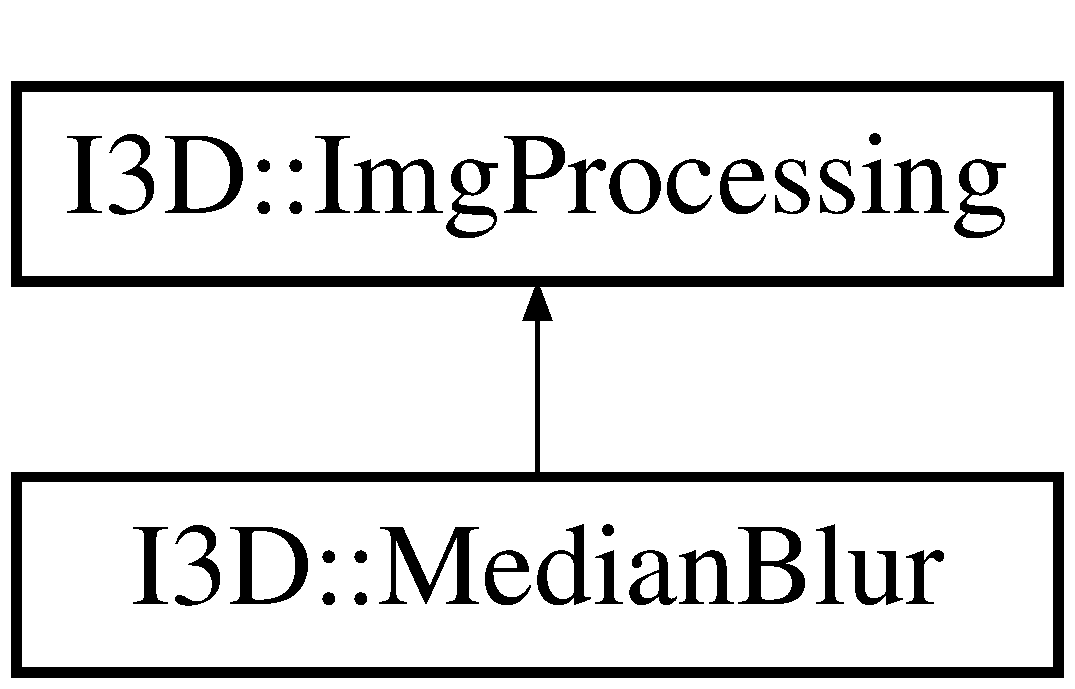
\includegraphics[height=2.000000cm]{class_i3_d_1_1_median_blur}
\end{center}
\end{figure}
\subsection*{Métodos públicos}
\begin{DoxyCompactItemize}
\item 
\hyperlink{class_i3_d_1_1_median_blur_ad3e65c0ebb97114038d1048340b06f51}{Median\+Blur} (int ksize)
\begin{DoxyCompactList}\small\item\em Constructora. \end{DoxyCompactList}\item 
int \hyperlink{class_i3_d_1_1_median_blur_aae49eae3c8ceda4ba3a2c485d2a64b4d}{execute} (const cv\+::\+Mat \&mat\+In, cv\+::\+Mat $\ast$mat\+Out) const  override
\begin{DoxyCompactList}\small\item\em Ejecuta el proceso. \end{DoxyCompactList}\item 
void \hyperlink{class_i3_d_1_1_median_blur_ac49b2d8067b0486d63723b739a7ee99b}{set\+Parameters} (int ksize)
\begin{DoxyCompactList}\small\item\em Establece los parámetros. \end{DoxyCompactList}\end{DoxyCompactItemize}
\subsection*{Otros miembros heredados}


\subsection{Descripción detallada}
Filtro de media Suaviza una imagen con un filtro de media. 

\subsection{Documentación del constructor y destructor}
\index{I3\+D\+::\+Median\+Blur@{I3\+D\+::\+Median\+Blur}!Median\+Blur@{Median\+Blur}}
\index{Median\+Blur@{Median\+Blur}!I3\+D\+::\+Median\+Blur@{I3\+D\+::\+Median\+Blur}}
\subsubsection[{\texorpdfstring{Median\+Blur(int ksize)}{MedianBlur(int ksize)}}]{\setlength{\rightskip}{0pt plus 5cm}I3\+D\+::\+Median\+Blur\+::\+Median\+Blur (
\begin{DoxyParamCaption}
\item[{int}]{ksize}
\end{DoxyParamCaption}
)\hspace{0.3cm}{\ttfamily [inline]}}\hypertarget{class_i3_d_1_1_median_blur_ad3e65c0ebb97114038d1048340b06f51}{}\label{class_i3_d_1_1_median_blur_ad3e65c0ebb97114038d1048340b06f51}


Constructora. 


\begin{DoxyParams}{Parámetros}
{\em ksize} & Tamaño del filtro \\
\hline
\end{DoxyParams}


\subsection{Documentación de las funciones miembro}
\index{I3\+D\+::\+Median\+Blur@{I3\+D\+::\+Median\+Blur}!execute@{execute}}
\index{execute@{execute}!I3\+D\+::\+Median\+Blur@{I3\+D\+::\+Median\+Blur}}
\subsubsection[{\texorpdfstring{execute(const cv\+::\+Mat \&mat\+In, cv\+::\+Mat $\ast$mat\+Out) const  override}{execute(const cv::Mat &matIn, cv::Mat *matOut) const  override}}]{\setlength{\rightskip}{0pt plus 5cm}int I3\+D\+::\+Median\+Blur\+::execute (
\begin{DoxyParamCaption}
\item[{const cv\+::\+Mat \&}]{mat\+In, }
\item[{cv\+::\+Mat $\ast$}]{mat\+Out}
\end{DoxyParamCaption}
) const\hspace{0.3cm}{\ttfamily [override]}, {\ttfamily [virtual]}}\hypertarget{class_i3_d_1_1_median_blur_aae49eae3c8ceda4ba3a2c485d2a64b4d}{}\label{class_i3_d_1_1_median_blur_aae49eae3c8ceda4ba3a2c485d2a64b4d}


Ejecuta el proceso. 


\begin{DoxyParams}[1]{Parámetros}
\mbox{\tt in}  & {\em mat\+In} & Imagen de entrada \\
\hline
\mbox{\tt out}  & {\em mat\+Out} & Imagen de salida \\
\hline
\end{DoxyParams}
\begin{DoxyReturn}{Devuelve}
Error. Si los procesos se ejecutan correctamente devuelve 0. 
\end{DoxyReturn}


Implementa \hyperlink{class_i3_d_1_1_img_processing_a74195f05bbf034566e9ff6e10f3af4c9}{I3\+D\+::\+Img\+Processing}.

\index{I3\+D\+::\+Median\+Blur@{I3\+D\+::\+Median\+Blur}!set\+Parameters@{set\+Parameters}}
\index{set\+Parameters@{set\+Parameters}!I3\+D\+::\+Median\+Blur@{I3\+D\+::\+Median\+Blur}}
\subsubsection[{\texorpdfstring{set\+Parameters(int ksize)}{setParameters(int ksize)}}]{\setlength{\rightskip}{0pt plus 5cm}void I3\+D\+::\+Median\+Blur\+::set\+Parameters (
\begin{DoxyParamCaption}
\item[{int}]{ksize}
\end{DoxyParamCaption}
)}\hypertarget{class_i3_d_1_1_median_blur_ac49b2d8067b0486d63723b739a7ee99b}{}\label{class_i3_d_1_1_median_blur_ac49b2d8067b0486d63723b739a7ee99b}


Establece los parámetros. 


\begin{DoxyParams}[1]{Parámetros}
\mbox{\tt in}  & {\em ksize} & Tamaño del filtro \\
\hline
\end{DoxyParams}


La documentación para esta clase fue generada a partir de los siguientes ficheros\+:\begin{DoxyCompactItemize}
\item 
C\+:/\+Desarrollo/tidop/src/\hyperlink{_img_processing_8h}{Img\+Processing.\+h}\item 
C\+:/\+Desarrollo/tidop/src/\hyperlink{_img_processing_8cpp}{Img\+Processing.\+cpp}\end{DoxyCompactItemize}

\hypertarget{class_i3_d_1_1_message}{}\section{Referencia de la Clase I3D\+:\+:Message}
\label{class_i3_d_1_1_message}\index{I3\+D\+::\+Message@{I3\+D\+::\+Message}}


\hyperlink{class_i3_d_1_1_message}{Message}.  




{\ttfamily \#include $<$messages.\+h$>$}

\subsection*{Métodos públicos}
\begin{DoxyCompactItemize}
\item 
\hyperlink{class_i3_d_1_1_message_a96370615d50060b3c7326da6374887ef}{$\sim$\+Message} ()
\item 
\hyperlink{class_i3_d_1_1_message_af1da7ef3a7ce40e79c298b1ebc9c2796}{Message} (\hyperlink{class_i3_d_1_1_message}{Message} const \&)=delete
\item 
void \hyperlink{class_i3_d_1_1_message_a7a757579a6966a8a80aeac7529a34b4b}{operator=} (\hyperlink{class_i3_d_1_1_message}{Message} const \&)=delete
\item 
\hyperlink{namespace_i3_d_a1c1740d2076e09b1a37b82e45a0327b5}{Message\+Level} \hyperlink{class_i3_d_1_1_message_aa5360e772b5fd6921bd4e8b3ec6925d8}{get\+Message\+Level} () const 
\begin{DoxyCompactList}\small\item\em Nivel de información de los mensajes. \end{DoxyCompactList}\item 
\hyperlink{class_i3_d_1_1_enum_flags}{Enum\+Flags}$<$ \hyperlink{namespace_i3_d_a2ccb65ac6e08844c1175a235107fa103}{Message\+Output} $>$ \hyperlink{class_i3_d_1_1_message_a9b6daa0dce23d8af3f774e9bcc1edc68}{get\+Message\+Output} () const 
\begin{DoxyCompactList}\small\item\em Nivel de información de los mensajes. \end{DoxyCompactList}\end{DoxyCompactItemize}
\subsection*{Métodos públicos estáticos}
\begin{DoxyCompactItemize}
\item 
static \hyperlink{class_i3_d_1_1_message}{Message} \& \hyperlink{class_i3_d_1_1_message_a4e67294cda784d09467939c4a580cf18}{get} ()
\begin{DoxyCompactList}\small\item\em Singleton para obtener una referencia única. \end{DoxyCompactList}\item 
static \hyperlink{class_i3_d_1_1_message}{Message} \& \hyperlink{class_i3_d_1_1_message_a525f877a41a1e7493188b2b720d1d254}{message} (const char $\ast$msg,...)
\begin{DoxyCompactList}\small\item\em message \end{DoxyCompactList}\item 
static void \hyperlink{class_i3_d_1_1_message_a414c9296d819d4ea29cbcb8719d1af2a}{print} ()
\begin{DoxyCompactList}\small\item\em Imprime un mensaje con las opciones establecidas. \end{DoxyCompactList}\item 
static void \hyperlink{class_i3_d_1_1_message_abcbe6bb4eaedadfc2a293bc30199b154}{print} (const \hyperlink{namespace_i3_d_a1c1740d2076e09b1a37b82e45a0327b5}{Message\+Level} \&level, const \hyperlink{namespace_i3_d_a2ccb65ac6e08844c1175a235107fa103}{Message\+Output} \&output)
\begin{DoxyCompactList}\small\item\em Imprime un mensaje. \end{DoxyCompactList}\item 
static void \hyperlink{class_i3_d_1_1_message_a35685ab8b54377a7846917cf065288cf}{print} (const \hyperlink{namespace_i3_d_a1c1740d2076e09b1a37b82e45a0327b5}{Message\+Level} \&level, const \hyperlink{namespace_i3_d_a2ccb65ac6e08844c1175a235107fa103}{Message\+Output} \&output, const char $\ast$file, int line, const char $\ast$function)
\begin{DoxyCompactList}\small\item\em Imprime un mensaje. \end{DoxyCompactList}\item 
static void \hyperlink{class_i3_d_1_1_message_a05802b639ffc072d4921757a7f494fad}{set\+Message\+Level} (const \hyperlink{namespace_i3_d_a1c1740d2076e09b1a37b82e45a0327b5}{Message\+Level} \&level)
\begin{DoxyCompactList}\small\item\em Establece el nivel de información de los mensajes. \end{DoxyCompactList}\item 
static void \hyperlink{class_i3_d_1_1_message_a423efa96869839dbb3ae772b58e055a0}{set\+Message\+Output} (const \hyperlink{namespace_i3_d_a2ccb65ac6e08844c1175a235107fa103}{Message\+Output} \&output)
\begin{DoxyCompactList}\small\item\em Establece la salida del mensaje. \end{DoxyCompactList}\item 
static void \hyperlink{class_i3_d_1_1_message_ab31745e88a79e1101b047232decd41c6}{set\+Time\+Log\+Format} (const std\+::string time\+Template)
\begin{DoxyCompactList}\small\item\em set\+Time\+Log\+Format \end{DoxyCompactList}\end{DoxyCompactItemize}


\subsection{Descripción detallada}
\hyperlink{class_i3_d_1_1_message}{Message}. 

\subsection{Documentación del constructor y destructor}
\index{I3\+D\+::\+Message@{I3\+D\+::\+Message}!````~Message@{$\sim$\+Message}}
\index{````~Message@{$\sim$\+Message}!I3\+D\+::\+Message@{I3\+D\+::\+Message}}
\subsubsection[{\texorpdfstring{$\sim$\+Message()}{~Message()}}]{\setlength{\rightskip}{0pt plus 5cm}I3\+D\+::\+Message\+::$\sim$\+Message (
\begin{DoxyParamCaption}
{}
\end{DoxyParamCaption}
)\hspace{0.3cm}{\ttfamily [inline]}}\hypertarget{class_i3_d_1_1_message_a96370615d50060b3c7326da6374887ef}{}\label{class_i3_d_1_1_message_a96370615d50060b3c7326da6374887ef}
Destructora \index{I3\+D\+::\+Message@{I3\+D\+::\+Message}!Message@{Message}}
\index{Message@{Message}!I3\+D\+::\+Message@{I3\+D\+::\+Message}}
\subsubsection[{\texorpdfstring{Message(\+Message const \&)=delete}{Message(Message const &)=delete}}]{\setlength{\rightskip}{0pt plus 5cm}I3\+D\+::\+Message\+::\+Message (
\begin{DoxyParamCaption}
\item[{{\bf Message} const \&}]{}
\end{DoxyParamCaption}
)\hspace{0.3cm}{\ttfamily [delete]}}\hypertarget{class_i3_d_1_1_message_af1da7ef3a7ce40e79c298b1ebc9c2796}{}\label{class_i3_d_1_1_message_af1da7ef3a7ce40e79c298b1ebc9c2796}


\subsection{Documentación de las funciones miembro}
\index{I3\+D\+::\+Message@{I3\+D\+::\+Message}!get@{get}}
\index{get@{get}!I3\+D\+::\+Message@{I3\+D\+::\+Message}}
\subsubsection[{\texorpdfstring{get()}{get()}}]{\setlength{\rightskip}{0pt plus 5cm}{\bf Message} \& I3\+D\+::\+Message\+::get (
\begin{DoxyParamCaption}
{}
\end{DoxyParamCaption}
)\hspace{0.3cm}{\ttfamily [static]}}\hypertarget{class_i3_d_1_1_message_a4e67294cda784d09467939c4a580cf18}{}\label{class_i3_d_1_1_message_a4e67294cda784d09467939c4a580cf18}


Singleton para obtener una referencia única. 

\index{I3\+D\+::\+Message@{I3\+D\+::\+Message}!get\+Message\+Level@{get\+Message\+Level}}
\index{get\+Message\+Level@{get\+Message\+Level}!I3\+D\+::\+Message@{I3\+D\+::\+Message}}
\subsubsection[{\texorpdfstring{get\+Message\+Level() const }{getMessageLevel() const }}]{\setlength{\rightskip}{0pt plus 5cm}{\bf Message\+Level} I3\+D\+::\+Message\+::get\+Message\+Level (
\begin{DoxyParamCaption}
{}
\end{DoxyParamCaption}
) const}\hypertarget{class_i3_d_1_1_message_aa5360e772b5fd6921bd4e8b3ec6925d8}{}\label{class_i3_d_1_1_message_aa5360e772b5fd6921bd4e8b3ec6925d8}


Nivel de información de los mensajes. 

\begin{DoxyReturn}{Devuelve}
Nivel de información de los mensajes 
\end{DoxyReturn}
\begin{DoxySeeAlso}{Ver también}
\hyperlink{namespace_i3_d_a1c1740d2076e09b1a37b82e45a0327b5}{Message\+Level} 
\end{DoxySeeAlso}
\index{I3\+D\+::\+Message@{I3\+D\+::\+Message}!get\+Message\+Output@{get\+Message\+Output}}
\index{get\+Message\+Output@{get\+Message\+Output}!I3\+D\+::\+Message@{I3\+D\+::\+Message}}
\subsubsection[{\texorpdfstring{get\+Message\+Output() const }{getMessageOutput() const }}]{\setlength{\rightskip}{0pt plus 5cm}{\bf Enum\+Flags}$<$ {\bf Message\+Output} $>$ I3\+D\+::\+Message\+::get\+Message\+Output (
\begin{DoxyParamCaption}
{}
\end{DoxyParamCaption}
) const}\hypertarget{class_i3_d_1_1_message_a9b6daa0dce23d8af3f774e9bcc1edc68}{}\label{class_i3_d_1_1_message_a9b6daa0dce23d8af3f774e9bcc1edc68}


Nivel de información de los mensajes. 

\begin{DoxyReturn}{Devuelve}
Nivel de información de los mensajes 
\end{DoxyReturn}
\begin{DoxySeeAlso}{Ver también}
\hyperlink{namespace_i3_d_a2ccb65ac6e08844c1175a235107fa103}{Message\+Output} 
\end{DoxySeeAlso}
\index{I3\+D\+::\+Message@{I3\+D\+::\+Message}!message@{message}}
\index{message@{message}!I3\+D\+::\+Message@{I3\+D\+::\+Message}}
\subsubsection[{\texorpdfstring{message(const char $\ast$msg,...)}{message(const char *msg,...)}}]{\setlength{\rightskip}{0pt plus 5cm}{\bf Message} \& I3\+D\+::\+Message\+::message (
\begin{DoxyParamCaption}
\item[{const char $\ast$}]{msg, }
\item[{}]{...}
\end{DoxyParamCaption}
)\hspace{0.3cm}{\ttfamily [static]}}\hypertarget{class_i3_d_1_1_message_a525f877a41a1e7493188b2b720d1d254}{}\label{class_i3_d_1_1_message_a525f877a41a1e7493188b2b720d1d254}


message 


\begin{DoxyParams}[1]{Parámetros}
\mbox{\tt in}  & {\em msg} & \\
\hline
\end{DoxyParams}
\begin{DoxyReturn}{Devuelve}

\end{DoxyReturn}
\index{I3\+D\+::\+Message@{I3\+D\+::\+Message}!operator=@{operator=}}
\index{operator=@{operator=}!I3\+D\+::\+Message@{I3\+D\+::\+Message}}
\subsubsection[{\texorpdfstring{operator=(\+Message const \&)=delete}{operator=(Message const &)=delete}}]{\setlength{\rightskip}{0pt plus 5cm}void I3\+D\+::\+Message\+::operator= (
\begin{DoxyParamCaption}
\item[{{\bf Message} const \&}]{}
\end{DoxyParamCaption}
)\hspace{0.3cm}{\ttfamily [delete]}}\hypertarget{class_i3_d_1_1_message_a7a757579a6966a8a80aeac7529a34b4b}{}\label{class_i3_d_1_1_message_a7a757579a6966a8a80aeac7529a34b4b}
\index{I3\+D\+::\+Message@{I3\+D\+::\+Message}!print@{print}}
\index{print@{print}!I3\+D\+::\+Message@{I3\+D\+::\+Message}}
\subsubsection[{\texorpdfstring{print()}{print()}}]{\setlength{\rightskip}{0pt plus 5cm}void I3\+D\+::\+Message\+::print (
\begin{DoxyParamCaption}
{}
\end{DoxyParamCaption}
)\hspace{0.3cm}{\ttfamily [static]}}\hypertarget{class_i3_d_1_1_message_a414c9296d819d4ea29cbcb8719d1af2a}{}\label{class_i3_d_1_1_message_a414c9296d819d4ea29cbcb8719d1af2a}


Imprime un mensaje con las opciones establecidas. 

\index{I3\+D\+::\+Message@{I3\+D\+::\+Message}!print@{print}}
\index{print@{print}!I3\+D\+::\+Message@{I3\+D\+::\+Message}}
\subsubsection[{\texorpdfstring{print(const Message\+Level \&level, const Message\+Output \&output)}{print(const MessageLevel &level, const MessageOutput &output)}}]{\setlength{\rightskip}{0pt plus 5cm}void I3\+D\+::\+Message\+::print (
\begin{DoxyParamCaption}
\item[{const {\bf Message\+Level} \&}]{level, }
\item[{const {\bf Message\+Output} \&}]{output}
\end{DoxyParamCaption}
)\hspace{0.3cm}{\ttfamily [static]}}\hypertarget{class_i3_d_1_1_message_abcbe6bb4eaedadfc2a293bc30199b154}{}\label{class_i3_d_1_1_message_abcbe6bb4eaedadfc2a293bc30199b154}


Imprime un mensaje. 


\begin{DoxyParams}[1]{Parámetros}
\mbox{\tt in}  & {\em level} & Nivel del mensaje \\
\hline
\mbox{\tt in}  & {\em output} & Tipo de salida \\
\hline
\end{DoxyParams}
\begin{DoxySeeAlso}{Ver también}
\hyperlink{namespace_i3_d_a1c1740d2076e09b1a37b82e45a0327b5}{Message\+Level}, \hyperlink{namespace_i3_d_a2ccb65ac6e08844c1175a235107fa103}{Message\+Output} 
\end{DoxySeeAlso}
\index{I3\+D\+::\+Message@{I3\+D\+::\+Message}!print@{print}}
\index{print@{print}!I3\+D\+::\+Message@{I3\+D\+::\+Message}}
\subsubsection[{\texorpdfstring{print(const Message\+Level \&level, const Message\+Output \&output, const char $\ast$file, int line, const char $\ast$function)}{print(const MessageLevel &level, const MessageOutput &output, const char *file, int line, const char *function)}}]{\setlength{\rightskip}{0pt plus 5cm}void I3\+D\+::\+Message\+::print (
\begin{DoxyParamCaption}
\item[{const {\bf Message\+Level} \&}]{level, }
\item[{const {\bf Message\+Output} \&}]{output, }
\item[{const char $\ast$}]{file, }
\item[{int}]{line, }
\item[{const char $\ast$}]{function}
\end{DoxyParamCaption}
)\hspace{0.3cm}{\ttfamily [static]}}\hypertarget{class_i3_d_1_1_message_a35685ab8b54377a7846917cf065288cf}{}\label{class_i3_d_1_1_message_a35685ab8b54377a7846917cf065288cf}


Imprime un mensaje. 


\begin{DoxyParams}[1]{Parámetros}
\mbox{\tt in}  & {\em level} & Nivel del mensaje \\
\hline
\mbox{\tt in}  & {\em output} & Tipo de salida \\
\hline
\mbox{\tt in}  & {\em file} & Nombre del fichero \\
\hline
\mbox{\tt in}  & {\em line} & Número de línea \\
\hline
\mbox{\tt in}  & {\em function} & Nombre de función \\
\hline
\end{DoxyParams}
\index{I3\+D\+::\+Message@{I3\+D\+::\+Message}!set\+Message\+Level@{set\+Message\+Level}}
\index{set\+Message\+Level@{set\+Message\+Level}!I3\+D\+::\+Message@{I3\+D\+::\+Message}}
\subsubsection[{\texorpdfstring{set\+Message\+Level(const Message\+Level \&level)}{setMessageLevel(const MessageLevel &level)}}]{\setlength{\rightskip}{0pt plus 5cm}void I3\+D\+::\+Message\+::set\+Message\+Level (
\begin{DoxyParamCaption}
\item[{const {\bf Message\+Level} \&}]{level}
\end{DoxyParamCaption}
)\hspace{0.3cm}{\ttfamily [static]}}\hypertarget{class_i3_d_1_1_message_a05802b639ffc072d4921757a7f494fad}{}\label{class_i3_d_1_1_message_a05802b639ffc072d4921757a7f494fad}


Establece el nivel de información de los mensajes. 


\begin{DoxyParams}[1]{Parámetros}
\mbox{\tt in}  & {\em level} & Nombre del fichero log. \\
\hline
\end{DoxyParams}
\begin{DoxySeeAlso}{Ver también}
\hyperlink{namespace_i3_d_a1c1740d2076e09b1a37b82e45a0327b5}{Message\+Level} 
\end{DoxySeeAlso}
\index{I3\+D\+::\+Message@{I3\+D\+::\+Message}!set\+Message\+Output@{set\+Message\+Output}}
\index{set\+Message\+Output@{set\+Message\+Output}!I3\+D\+::\+Message@{I3\+D\+::\+Message}}
\subsubsection[{\texorpdfstring{set\+Message\+Output(const Message\+Output \&output)}{setMessageOutput(const MessageOutput &output)}}]{\setlength{\rightskip}{0pt plus 5cm}void I3\+D\+::\+Message\+::set\+Message\+Output (
\begin{DoxyParamCaption}
\item[{const {\bf Message\+Output} \&}]{output}
\end{DoxyParamCaption}
)\hspace{0.3cm}{\ttfamily [static]}}\hypertarget{class_i3_d_1_1_message_a423efa96869839dbb3ae772b58e055a0}{}\label{class_i3_d_1_1_message_a423efa96869839dbb3ae772b58e055a0}


Establece la salida del mensaje. 


\begin{DoxyParams}[1]{Parámetros}
\mbox{\tt in}  & {\em output} & Salida del mensaje \\
\hline
\end{DoxyParams}
\begin{DoxySeeAlso}{Ver también}
\hyperlink{namespace_i3_d_a2ccb65ac6e08844c1175a235107fa103}{Message\+Output} 
\end{DoxySeeAlso}
\index{I3\+D\+::\+Message@{I3\+D\+::\+Message}!set\+Time\+Log\+Format@{set\+Time\+Log\+Format}}
\index{set\+Time\+Log\+Format@{set\+Time\+Log\+Format}!I3\+D\+::\+Message@{I3\+D\+::\+Message}}
\subsubsection[{\texorpdfstring{set\+Time\+Log\+Format(const std\+::string time\+Template)}{setTimeLogFormat(const std::string timeTemplate)}}]{\setlength{\rightskip}{0pt plus 5cm}void I3\+D\+::\+Message\+::set\+Time\+Log\+Format (
\begin{DoxyParamCaption}
\item[{const std\+::string}]{time\+Template}
\end{DoxyParamCaption}
)\hspace{0.3cm}{\ttfamily [static]}}\hypertarget{class_i3_d_1_1_message_ab31745e88a79e1101b047232decd41c6}{}\label{class_i3_d_1_1_message_ab31745e88a79e1101b047232decd41c6}


set\+Time\+Log\+Format 


\begin{DoxyCode}
\hyperlink{class_i3_d_1_1_message_ab31745e88a79e1101b047232decd41c6}{Message::setTimeLogFormat}( \textcolor{stringliteral}{"%d - %b - %Y (%H:%M:%S)"} );
\end{DoxyCode}
 
\begin{DoxyParams}[1]{Parámetros}
\mbox{\tt in}  & {\em time\+Template} & \\
\hline
\end{DoxyParams}


La documentación para esta clase fue generada a partir de los siguientes ficheros\+:\begin{DoxyCompactItemize}
\item 
C\+:/\+Desarrollo/tidop/src/core/\hyperlink{messages_8h}{messages.\+h}\item 
C\+:/\+Desarrollo/tidop/src/core/\hyperlink{messages_8cpp}{messages.\+cpp}\end{DoxyCompactItemize}

\hypertarget{class_i3_d_1_1morphological_operation}{}\section{Referencia de la Clase I3D\+:\+:morphological\+Operation}
\label{class_i3_d_1_1morphological_operation}\index{I3\+D\+::morphological\+Operation@{I3\+D\+::morphological\+Operation}}


Clase base para las operaciones morfológicas.  




{\ttfamily \#include $<$Img\+Processing.\+h$>$}

Diagrama de herencias de I3D\+:\+:morphological\+Operation\begin{figure}[H]
\begin{center}
\leavevmode
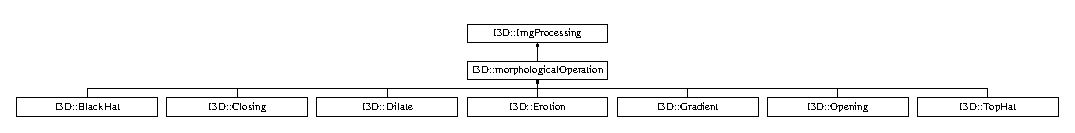
\includegraphics[height=1.333333cm]{class_i3_d_1_1morphological_operation}
\end{center}
\end{figure}
\subsection*{Métodos públicos}
\begin{DoxyCompactItemize}
\item 
\hyperlink{class_i3_d_1_1morphological_operation_adccfcde6d2223d29dd6c7190cb4b4c23}{morphological\+Operation} (\hyperlink{group___img_proc_gaa7be5aaaa0e9ec5885c5bd72f41dad47}{process\+\_\+type} \hyperlink{class_i3_d_1_1_img_processing_af87bd3404d91bca669b04af1f45cbff0}{type})
\begin{DoxyCompactList}\small\item\em Constructora de la clase. \end{DoxyCompactList}\item 
virtual \hyperlink{class_i3_d_1_1morphological_operation_a21bb0f558a0c0d2c670393ec84be231f}{$\sim$morphological\+Operation} ()
\begin{DoxyCompactList}\small\item\em Destuctora. \end{DoxyCompactList}\item 
int \hyperlink{class_i3_d_1_1morphological_operation_aafa533c5999bed3e9d4680a6434cb43e}{execute} (const cv\+::\+Mat \&mat\+In, cv\+::\+Mat $\ast$mat\+Out) const  override
\begin{DoxyCompactList}\small\item\em Ejecuta el proceso Metodo virtual puro que deben implementar las clases hijas. \end{DoxyCompactList}\item 
void \hyperlink{class_i3_d_1_1morphological_operation_adb431685feba88a87c71d13e1e3b2ce2}{set\+Parameters} (int size, cv\+::\+Morph\+Shapes shapes=cv\+::\+M\+O\+R\+P\+H\+\_\+\+R\+E\+CT, cv\+::\+Point anchor=cv\+::\+Point(-\/1,-\/1), int iterations=1, int border\+Type=cv\+::\+B\+O\+R\+D\+E\+R\+\_\+\+C\+O\+N\+S\+T\+A\+NT, const cv\+::\+Scalar \&border\+Value=cv\+::morphology\+Default\+Border\+Value())
\begin{DoxyCompactList}\small\item\em Establece los parámetros. \end{DoxyCompactList}\end{DoxyCompactItemize}
\subsection*{Atributos protegidos}
\begin{DoxyCompactItemize}
\item 
cv\+::\+Morph\+Shapes \hyperlink{class_i3_d_1_1morphological_operation_a15b21c649cbb7f4f86625005c2390be3}{m\+Shapes}
\begin{DoxyCompactList}\small\item\em Forma del elemento estructurante. \end{DoxyCompactList}\item 
int \hyperlink{class_i3_d_1_1morphological_operation_a704f5eda2852dfdb30ef54f92d936e5a}{m\+Size}
\begin{DoxyCompactList}\small\item\em dilation\+Size \end{DoxyCompactList}\item 
cv\+::\+Point \hyperlink{class_i3_d_1_1morphological_operation_aea6a98ce1ee4c1a0f9767c227bd01988}{m\+Anchor}
\begin{DoxyCompactList}\small\item\em Punto de anclaje. Por defecto es el centro del kernel. \end{DoxyCompactList}\item 
int \hyperlink{class_i3_d_1_1morphological_operation_a559f56b17ef0ebbbba5e5a88c3bb113a}{m\+Iterations}
\begin{DoxyCompactList}\small\item\em Número de veces que se aplica la dilatación. \end{DoxyCompactList}\item 
int \hyperlink{class_i3_d_1_1morphological_operation_ae160ad01e68f62492633324306b87cb5}{m\+Border\+Type}
\begin{DoxyCompactList}\small\item\em Método de extrapolación de pixeles. \end{DoxyCompactList}\item 
cv\+::\+Scalar \hyperlink{class_i3_d_1_1morphological_operation_a9af41bcd3b3e9c5d44bbfdc31a707a9c}{m\+Border\+Value}
\begin{DoxyCompactList}\small\item\em Valor de borde en el caso de un borde constante. \end{DoxyCompactList}\end{DoxyCompactItemize}
\subsection*{Otros miembros heredados}


\subsection{Descripción detallada}
Clase base para las operaciones morfológicas. 

Operaciones morfologicas básicas\+:~\newline
 \begin{DoxyItemize}
\item Erosion (\hyperlink{class_i3_d_1_1_erotion}{Erotion}) \item Dilatacion (\hyperlink{class_i3_d_1_1_dilate}{Dilate})\end{DoxyItemize}
Operaciones morfologicas avanzadas (cv\+::morphology\+Ex)\+: \begin{DoxyItemize}
\item Apertura (\hyperlink{class_i3_d_1_1_opening}{Opening}) = erosion + dilation \item Cierre (\hyperlink{class_i3_d_1_1_closing}{Closing}) = dilatación + erosión \item Morphological \hyperlink{class_i3_d_1_1_gradient}{Gradient} = dilatación -\/ erosión \item \hyperlink{class_i3_d_1_1_top_hat}{Top\+Hat} = src -\/ apertura(src) \item \hyperlink{class_i3_d_1_1_black_hat}{Black\+Hat} = cierre(src) -\/ src \end{DoxyItemize}


\subsection{Documentación del constructor y destructor}
\index{I3\+D\+::morphological\+Operation@{I3\+D\+::morphological\+Operation}!morphological\+Operation@{morphological\+Operation}}
\index{morphological\+Operation@{morphological\+Operation}!I3\+D\+::morphological\+Operation@{I3\+D\+::morphological\+Operation}}
\subsubsection[{\texorpdfstring{morphological\+Operation(process\+\_\+type type)}{morphologicalOperation(process_type type)}}]{\setlength{\rightskip}{0pt plus 5cm}I3\+D\+::morphological\+Operation\+::morphological\+Operation (
\begin{DoxyParamCaption}
\item[{{\bf process\+\_\+type}}]{type}
\end{DoxyParamCaption}
)\hspace{0.3cm}{\ttfamily [inline]}}\hypertarget{class_i3_d_1_1morphological_operation_adccfcde6d2223d29dd6c7190cb4b4c23}{}\label{class_i3_d_1_1morphological_operation_adccfcde6d2223d29dd6c7190cb4b4c23}


Constructora de la clase. 


\begin{DoxyParams}[1]{Parámetros}
\mbox{\tt in}  & {\em type} & Tipo de proceso. \\
\hline
\end{DoxyParams}
\begin{DoxySeeAlso}{Ver también}
\hyperlink{group___img_proc_gaa7be5aaaa0e9ec5885c5bd72f41dad47}{process\+\_\+type} 
\end{DoxySeeAlso}
\index{I3\+D\+::morphological\+Operation@{I3\+D\+::morphological\+Operation}!````~morphological\+Operation@{$\sim$morphological\+Operation}}
\index{````~morphological\+Operation@{$\sim$morphological\+Operation}!I3\+D\+::morphological\+Operation@{I3\+D\+::morphological\+Operation}}
\subsubsection[{\texorpdfstring{$\sim$morphological\+Operation()}{~morphologicalOperation()}}]{\setlength{\rightskip}{0pt plus 5cm}virtual I3\+D\+::morphological\+Operation\+::$\sim$morphological\+Operation (
\begin{DoxyParamCaption}
{}
\end{DoxyParamCaption}
)\hspace{0.3cm}{\ttfamily [inline]}, {\ttfamily [virtual]}}\hypertarget{class_i3_d_1_1morphological_operation_a21bb0f558a0c0d2c670393ec84be231f}{}\label{class_i3_d_1_1morphological_operation_a21bb0f558a0c0d2c670393ec84be231f}


Destuctora. 



\subsection{Documentación de las funciones miembro}
\index{I3\+D\+::morphological\+Operation@{I3\+D\+::morphological\+Operation}!execute@{execute}}
\index{execute@{execute}!I3\+D\+::morphological\+Operation@{I3\+D\+::morphological\+Operation}}
\subsubsection[{\texorpdfstring{execute(const cv\+::\+Mat \&mat\+In, cv\+::\+Mat $\ast$mat\+Out) const  override}{execute(const cv::Mat &matIn, cv::Mat *matOut) const  override}}]{\setlength{\rightskip}{0pt plus 5cm}int I3\+D\+::morphological\+Operation\+::execute (
\begin{DoxyParamCaption}
\item[{const cv\+::\+Mat \&}]{mat\+In, }
\item[{cv\+::\+Mat $\ast$}]{mat\+Out}
\end{DoxyParamCaption}
) const\hspace{0.3cm}{\ttfamily [override]}, {\ttfamily [virtual]}}\hypertarget{class_i3_d_1_1morphological_operation_aafa533c5999bed3e9d4680a6434cb43e}{}\label{class_i3_d_1_1morphological_operation_aafa533c5999bed3e9d4680a6434cb43e}


Ejecuta el proceso Metodo virtual puro que deben implementar las clases hijas. 


\begin{DoxyParams}[1]{Parámetros}
\mbox{\tt in}  & {\em mat\+In} & Imagen de entrada \\
\hline
\mbox{\tt out}  & {\em mat\+Out} & Imagen de salida \\
\hline
\end{DoxyParams}
\begin{DoxyReturn}{Devuelve}
Error. Si los procesos se ejecutan correctamente devuelve 0. 
\end{DoxyReturn}


Implementa \hyperlink{class_i3_d_1_1_img_processing_a74195f05bbf034566e9ff6e10f3af4c9}{I3\+D\+::\+Img\+Processing}.

\index{I3\+D\+::morphological\+Operation@{I3\+D\+::morphological\+Operation}!set\+Parameters@{set\+Parameters}}
\index{set\+Parameters@{set\+Parameters}!I3\+D\+::morphological\+Operation@{I3\+D\+::morphological\+Operation}}
\subsubsection[{\texorpdfstring{set\+Parameters(int size, cv\+::\+Morph\+Shapes shapes=cv\+::\+M\+O\+R\+P\+H\+\_\+\+R\+E\+C\+T, cv\+::\+Point anchor=cv\+::\+Point(-\/1,-\/1), int iterations=1, int border\+Type=cv\+::\+B\+O\+R\+D\+E\+R\+\_\+\+C\+O\+N\+S\+T\+A\+N\+T, const cv\+::\+Scalar \&border\+Value=cv\+::morphology\+Default\+Border\+Value())}{setParameters(int size, cv::MorphShapes shapes=cv::MORPH_RECT, cv::Point anchor=cv::Point(-1,-1), int iterations=1, int borderType=cv::BORDER_CONSTANT, const cv::Scalar &borderValue=cv::morphologyDefaultBorderValue())}}]{\setlength{\rightskip}{0pt plus 5cm}void I3\+D\+::morphological\+Operation\+::set\+Parameters (
\begin{DoxyParamCaption}
\item[{int}]{size, }
\item[{cv\+::\+Morph\+Shapes}]{shapes = {\ttfamily cv\+:\+:MORPH\+\_\+RECT}, }
\item[{cv\+::\+Point}]{anchor = {\ttfamily cv\+:\+:Point(-\/1,~-\/1)}, }
\item[{int}]{iterations = {\ttfamily 1}, }
\item[{int}]{border\+Type = {\ttfamily cv\+:\+:BORDER\+\_\+CONSTANT}, }
\item[{const cv\+::\+Scalar \&}]{border\+Value = {\ttfamily cv\+:\+:morphologyDefaultBorderValue()}}
\end{DoxyParamCaption}
)}\hypertarget{class_i3_d_1_1morphological_operation_adb431685feba88a87c71d13e1e3b2ce2}{}\label{class_i3_d_1_1morphological_operation_adb431685feba88a87c71d13e1e3b2ce2}


Establece los parámetros. 


\begin{DoxyParams}[1]{Parámetros}
\mbox{\tt in}  & {\em size} & \\
\hline
\mbox{\tt in}  & {\em type} & \\
\hline
\mbox{\tt in}  & {\em anchor} & Punto de anclaje. Por defecto es el centro del kernel \\
\hline
\mbox{\tt in}  & {\em iterations} & \\
\hline
\mbox{\tt in}  & {\em border\+Type} & Método de extrapolación \\
\hline
\end{DoxyParams}


\subsection{Documentación de los datos miembro}
\index{I3\+D\+::morphological\+Operation@{I3\+D\+::morphological\+Operation}!m\+Anchor@{m\+Anchor}}
\index{m\+Anchor@{m\+Anchor}!I3\+D\+::morphological\+Operation@{I3\+D\+::morphological\+Operation}}
\subsubsection[{\texorpdfstring{m\+Anchor}{mAnchor}}]{\setlength{\rightskip}{0pt plus 5cm}cv\+::\+Point I3\+D\+::morphological\+Operation\+::m\+Anchor\hspace{0.3cm}{\ttfamily [protected]}}\hypertarget{class_i3_d_1_1morphological_operation_aea6a98ce1ee4c1a0f9767c227bd01988}{}\label{class_i3_d_1_1morphological_operation_aea6a98ce1ee4c1a0f9767c227bd01988}


Punto de anclaje. Por defecto es el centro del kernel. 

\index{I3\+D\+::morphological\+Operation@{I3\+D\+::morphological\+Operation}!m\+Border\+Type@{m\+Border\+Type}}
\index{m\+Border\+Type@{m\+Border\+Type}!I3\+D\+::morphological\+Operation@{I3\+D\+::morphological\+Operation}}
\subsubsection[{\texorpdfstring{m\+Border\+Type}{mBorderType}}]{\setlength{\rightskip}{0pt plus 5cm}int I3\+D\+::morphological\+Operation\+::m\+Border\+Type\hspace{0.3cm}{\ttfamily [protected]}}\hypertarget{class_i3_d_1_1morphological_operation_ae160ad01e68f62492633324306b87cb5}{}\label{class_i3_d_1_1morphological_operation_ae160ad01e68f62492633324306b87cb5}


Método de extrapolación de pixeles. 

\index{I3\+D\+::morphological\+Operation@{I3\+D\+::morphological\+Operation}!m\+Border\+Value@{m\+Border\+Value}}
\index{m\+Border\+Value@{m\+Border\+Value}!I3\+D\+::morphological\+Operation@{I3\+D\+::morphological\+Operation}}
\subsubsection[{\texorpdfstring{m\+Border\+Value}{mBorderValue}}]{\setlength{\rightskip}{0pt plus 5cm}cv\+::\+Scalar I3\+D\+::morphological\+Operation\+::m\+Border\+Value\hspace{0.3cm}{\ttfamily [protected]}}\hypertarget{class_i3_d_1_1morphological_operation_a9af41bcd3b3e9c5d44bbfdc31a707a9c}{}\label{class_i3_d_1_1morphological_operation_a9af41bcd3b3e9c5d44bbfdc31a707a9c}


Valor de borde en el caso de un borde constante. 

\index{I3\+D\+::morphological\+Operation@{I3\+D\+::morphological\+Operation}!m\+Iterations@{m\+Iterations}}
\index{m\+Iterations@{m\+Iterations}!I3\+D\+::morphological\+Operation@{I3\+D\+::morphological\+Operation}}
\subsubsection[{\texorpdfstring{m\+Iterations}{mIterations}}]{\setlength{\rightskip}{0pt plus 5cm}int I3\+D\+::morphological\+Operation\+::m\+Iterations\hspace{0.3cm}{\ttfamily [protected]}}\hypertarget{class_i3_d_1_1morphological_operation_a559f56b17ef0ebbbba5e5a88c3bb113a}{}\label{class_i3_d_1_1morphological_operation_a559f56b17ef0ebbbba5e5a88c3bb113a}


Número de veces que se aplica la dilatación. 

\index{I3\+D\+::morphological\+Operation@{I3\+D\+::morphological\+Operation}!m\+Shapes@{m\+Shapes}}
\index{m\+Shapes@{m\+Shapes}!I3\+D\+::morphological\+Operation@{I3\+D\+::morphological\+Operation}}
\subsubsection[{\texorpdfstring{m\+Shapes}{mShapes}}]{\setlength{\rightskip}{0pt plus 5cm}cv\+::\+Morph\+Shapes I3\+D\+::morphological\+Operation\+::m\+Shapes\hspace{0.3cm}{\ttfamily [protected]}}\hypertarget{class_i3_d_1_1morphological_operation_a15b21c649cbb7f4f86625005c2390be3}{}\label{class_i3_d_1_1morphological_operation_a15b21c649cbb7f4f86625005c2390be3}


Forma del elemento estructurante. 

\index{I3\+D\+::morphological\+Operation@{I3\+D\+::morphological\+Operation}!m\+Size@{m\+Size}}
\index{m\+Size@{m\+Size}!I3\+D\+::morphological\+Operation@{I3\+D\+::morphological\+Operation}}
\subsubsection[{\texorpdfstring{m\+Size}{mSize}}]{\setlength{\rightskip}{0pt plus 5cm}int I3\+D\+::morphological\+Operation\+::m\+Size\hspace{0.3cm}{\ttfamily [protected]}}\hypertarget{class_i3_d_1_1morphological_operation_a704f5eda2852dfdb30ef54f92d936e5a}{}\label{class_i3_d_1_1morphological_operation_a704f5eda2852dfdb30ef54f92d936e5a}


dilation\+Size 



La documentación para esta clase fue generada a partir de los siguientes ficheros\+:\begin{DoxyCompactItemize}
\item 
C\+:/\+Desarrollo/tidop/src/\hyperlink{_img_processing_8h}{Img\+Processing.\+h}\item 
C\+:/\+Desarrollo/tidop/src/\hyperlink{_img_processing_8cpp}{Img\+Processing.\+cpp}\end{DoxyCompactItemize}

\hypertarget{structmsg_properties}{}\section{Referencia de la Estructura msg\+Properties}
\label{structmsg_properties}\index{msg\+Properties@{msg\+Properties}}
\subsection*{Atributos públicos}
\begin{DoxyCompactItemize}
\item 
const char $\ast$ \hyperlink{structmsg_properties_a49cb74021371b7e2d47b04a8010e76a8}{normal}
\item 
const char $\ast$ \hyperlink{structmsg_properties_a9eb055af2fdf96afc626c6e8eb62442c}{extend}
\item 
unsigned short \hyperlink{structmsg_properties_a1ae1f972fd65ebe736a209a0f3c807fe}{fore\+Color}
\end{DoxyCompactItemize}


\subsection{Documentación de los datos miembro}
\index{msg\+Properties@{msg\+Properties}!extend@{extend}}
\index{extend@{extend}!msg\+Properties@{msg\+Properties}}
\subsubsection[{\texorpdfstring{extend}{extend}}]{\setlength{\rightskip}{0pt plus 5cm}const char$\ast$ msg\+Properties\+::extend}\hypertarget{structmsg_properties_a9eb055af2fdf96afc626c6e8eb62442c}{}\label{structmsg_properties_a9eb055af2fdf96afc626c6e8eb62442c}
\index{msg\+Properties@{msg\+Properties}!fore\+Color@{fore\+Color}}
\index{fore\+Color@{fore\+Color}!msg\+Properties@{msg\+Properties}}
\subsubsection[{\texorpdfstring{fore\+Color}{foreColor}}]{\setlength{\rightskip}{0pt plus 5cm}unsigned short msg\+Properties\+::fore\+Color}\hypertarget{structmsg_properties_a1ae1f972fd65ebe736a209a0f3c807fe}{}\label{structmsg_properties_a1ae1f972fd65ebe736a209a0f3c807fe}
\index{msg\+Properties@{msg\+Properties}!normal@{normal}}
\index{normal@{normal}!msg\+Properties@{msg\+Properties}}
\subsubsection[{\texorpdfstring{normal}{normal}}]{\setlength{\rightskip}{0pt plus 5cm}const char$\ast$ msg\+Properties\+::normal}\hypertarget{structmsg_properties_a49cb74021371b7e2d47b04a8010e76a8}{}\label{structmsg_properties_a49cb74021371b7e2d47b04a8010e76a8}


La documentación para esta estructura fue generada a partir del siguiente fichero\+:\begin{DoxyCompactItemize}
\item 
D\+:/\+Desarrollo/tidop/src/core/\hyperlink{messages_8cpp}{messages.\+cpp}\end{DoxyCompactItemize}

\hypertarget{class_i3_d_1_1_multi_point}{}\section{Referencia de la plantilla de la Clase I3D\+:\+:Multi\+Point$<$ T $>$}
\label{class_i3_d_1_1_multi_point}\index{I3\+D\+::\+Multi\+Point$<$ T $>$@{I3\+D\+::\+Multi\+Point$<$ T $>$}}


Clase multi-\/punto.  




{\ttfamily \#include $<$point.\+h$>$}

\subsection*{Tipos públicos}
\begin{DoxyCompactItemize}
\item 
typedef T \hyperlink{class_i3_d_1_1_multi_point_ae8bafa5f4c3f71c19b294e5495683582}{type}
\begin{DoxyCompactList}\small\item\em type \end{DoxyCompactList}\end{DoxyCompactItemize}
\subsection*{Métodos públicos}
\begin{DoxyCompactItemize}
\item 
\hyperlink{group___geometric_entities_ga15cd19a3ddf5a39c3154efe440dde6c7}{Multi\+Point} ()
\begin{DoxyCompactList}\small\item\em Constructora por defecto. \end{DoxyCompactList}\item 
\hyperlink{group___geometric_entities_ga5581044092b6db2870f35347c8af5b73}{Multi\+Point} (int size)
\begin{DoxyCompactList}\small\item\em Constructor que reserva tamaño para n puntos. \end{DoxyCompactList}\item 
\hyperlink{group___geometric_entities_gaadc33d9d15e6fe63040915f1f39d9b40}{Multi\+Point} (const \hyperlink{class_i3_d_1_1_multi_point}{Multi\+Point} \&multi\+Point)
\begin{DoxyCompactList}\small\item\em Constructor de copia. \end{DoxyCompactList}\item 
\hyperlink{group___geometric_entities_ga4f8daff9e4ffbfcb5f1cc670f4e3681c}{Multi\+Point} (const std\+::vector$<$ cv\+::\+Point\+\_\+$<$ T $>$$>$ \&v\+Point)
\begin{DoxyCompactList}\small\item\em Constructor. \end{DoxyCompactList}\item 
\hyperlink{group___geometric_entities_ga5e9b29cc4e72496e3c0df560bcaf39d4}{Multi\+Point} (std\+::initializer\+\_\+list$<$ cv\+::\+Point\+\_\+$<$ T $>$$>$ list\+Points)
\begin{DoxyCompactList}\small\item\em Constructor lista de inicialización. \end{DoxyCompactList}\item 
\hyperlink{class_i3_d_1_1_multi_point}{Multi\+Point} \& \hyperlink{group___geometric_entities_ga006fc08c663fc30e8f7f5dce0655bf96}{operator=} (const \hyperlink{class_i3_d_1_1_multi_point}{Multi\+Point} \&multi\+Point)
\begin{DoxyCompactList}\small\item\em Sobrecarga del operador de asignación. \end{DoxyCompactList}\item 
void \hyperlink{group___geometric_entities_ga9199a5fd8948e1f456cb0a47f72f99b7}{add} (const cv\+::\+Point\+\_\+$<$ T $>$ \&point)
\begin{DoxyCompactList}\small\item\em Añade un punto a la colección. \end{DoxyCompactList}\item 
const std\+::vector$<$ cv\+::\+Point\+\_\+$<$ T $>$ $>$ \& \hyperlink{class_i3_d_1_1_multi_point_a9b3d49d95f7ca38a48910eb9e419d6d7}{get\+Points} () const 
\begin{DoxyCompactList}\small\item\em Devuelve los puntos de la colección. \end{DoxyCompactList}\item 
std\+::vector$<$ cv\+::\+Point\+\_\+$<$ T $>$ $>$ \hyperlink{group___geometric_entities_ga2985cb5eede5d9631f87d50aaec4ca5c}{get\+Points\+In\+Window} (const \hyperlink{class_i3_d_1_1_window}{Window}$<$ T $>$ \&w) const 
\begin{DoxyCompactList}\small\item\em Devuelve los puntos que esta dentro de una ventana. \end{DoxyCompactList}\item 
int \hyperlink{class_i3_d_1_1_multi_point_a1ca5ac1c6908662f4df1b34cf70b2b17}{get\+Size} () const 
\begin{DoxyCompactList}\small\item\em Número de puntos de la colección. \end{DoxyCompactList}\item 
\hyperlink{class_i3_d_1_1_window}{Window}$<$ T $>$ \hyperlink{group___geometric_entities_ga25a83a5c3a0477ef6ee6c339cda6c4e7}{get\+Window} () const 
\begin{DoxyCompactList}\small\item\em Ventana envolvente. \end{DoxyCompactList}\item 
void \hyperlink{class_i3_d_1_1_multi_point_abb806a4c8c4e578f5ee440e1f30748a1}{resize} (int size)
\begin{DoxyCompactList}\small\item\em resize \end{DoxyCompactList}\item 
cv\+::\+Point\+\_\+$<$ T $>$ \& \hyperlink{class_i3_d_1_1_multi_point_a24be0acec8e96b6479675b4bfbd0f365}{operator\mbox{[}$\,$\mbox{]}} (size\+\_\+t id)
\begin{DoxyCompactList}\small\item\em Operador de indexación sobrecargado. \end{DoxyCompactList}\end{DoxyCompactItemize}


\subsection{Descripción detallada}
\subsubsection*{template$<$typename T$>$\\*
class I3\+D\+::\+Multi\+Point$<$ T $>$}

Clase multi-\/punto. 

Esta template representa un conjunto de puntos relaccionados que se agrupan en una misma entidad multipunto.

Se han definido los siguientes alias para facilitar el acceso\+: 
\begin{DoxyCode}
\textcolor{keyword}{typedef} MultiPoint<int> \hyperlink{group___geometric_entities_gacd97741d89ded5ad4fbe71d32309e62b}{MultiPointI};
\textcolor{keyword}{typedef} MultiPoint<double> \hyperlink{group___geometric_entities_ga17d41c547edd7b9a916383723c0aeaec}{MultiPointD};
\textcolor{keyword}{typedef} MultiPoint<float> \hyperlink{group___geometric_entities_ga7e19d99de4e64c17e396f090e87d438b}{MultiPointF};
\end{DoxyCode}
 

\subsection{Documentación de los \textquotesingle{}Typedef\textquotesingle{} miembros de la clase}
\index{I3\+D\+::\+Multi\+Point@{I3\+D\+::\+Multi\+Point}!type@{type}}
\index{type@{type}!I3\+D\+::\+Multi\+Point@{I3\+D\+::\+Multi\+Point}}
\subsubsection[{\texorpdfstring{type}{type}}]{\setlength{\rightskip}{0pt plus 5cm}template$<$typename T $>$ typedef T {\bf I3\+D\+::\+Multi\+Point}$<$ T $>$\+::{\bf type}}\hypertarget{class_i3_d_1_1_multi_point_ae8bafa5f4c3f71c19b294e5495683582}{}\label{class_i3_d_1_1_multi_point_ae8bafa5f4c3f71c19b294e5495683582}


type 



\subsection{Documentación de las funciones miembro}
\index{I3\+D\+::\+Multi\+Point@{I3\+D\+::\+Multi\+Point}!get\+Points@{get\+Points}}
\index{get\+Points@{get\+Points}!I3\+D\+::\+Multi\+Point@{I3\+D\+::\+Multi\+Point}}
\subsubsection[{\texorpdfstring{get\+Points() const }{getPoints() const }}]{\setlength{\rightskip}{0pt plus 5cm}template$<$typename T $>$ const std\+::vector$<$cv\+::\+Point\+\_\+$<$T$>$ $>$\& {\bf I3\+D\+::\+Multi\+Point}$<$ T $>$\+::get\+Points (
\begin{DoxyParamCaption}
{}
\end{DoxyParamCaption}
) const\hspace{0.3cm}{\ttfamily [inline]}}\hypertarget{class_i3_d_1_1_multi_point_a9b3d49d95f7ca38a48910eb9e419d6d7}{}\label{class_i3_d_1_1_multi_point_a9b3d49d95f7ca38a48910eb9e419d6d7}


Devuelve los puntos de la colección. 

\begin{DoxyReturn}{Devuelve}
vector de puntos 
\end{DoxyReturn}
\index{I3\+D\+::\+Multi\+Point@{I3\+D\+::\+Multi\+Point}!get\+Size@{get\+Size}}
\index{get\+Size@{get\+Size}!I3\+D\+::\+Multi\+Point@{I3\+D\+::\+Multi\+Point}}
\subsubsection[{\texorpdfstring{get\+Size() const }{getSize() const }}]{\setlength{\rightskip}{0pt plus 5cm}template$<$typename T $>$ int {\bf I3\+D\+::\+Multi\+Point}$<$ T $>$\+::get\+Size (
\begin{DoxyParamCaption}
{}
\end{DoxyParamCaption}
) const\hspace{0.3cm}{\ttfamily [inline]}}\hypertarget{class_i3_d_1_1_multi_point_a1ca5ac1c6908662f4df1b34cf70b2b17}{}\label{class_i3_d_1_1_multi_point_a1ca5ac1c6908662f4df1b34cf70b2b17}


Número de puntos de la colección. 

\begin{DoxyReturn}{Devuelve}
Número de puntos 
\end{DoxyReturn}
\index{I3\+D\+::\+Multi\+Point@{I3\+D\+::\+Multi\+Point}!operator\mbox{[}$\,$\mbox{]}@{operator[]}}
\index{operator\mbox{[}$\,$\mbox{]}@{operator[]}!I3\+D\+::\+Multi\+Point@{I3\+D\+::\+Multi\+Point}}
\subsubsection[{\texorpdfstring{operator[](size\+\_\+t id)}{operator[](size_t id)}}]{\setlength{\rightskip}{0pt plus 5cm}template$<$typename T $>$ cv\+::\+Point\+\_\+$<$T$>$\& {\bf I3\+D\+::\+Multi\+Point}$<$ T $>$\+::operator\mbox{[}$\,$\mbox{]} (
\begin{DoxyParamCaption}
\item[{size\+\_\+t}]{id}
\end{DoxyParamCaption}
)\hspace{0.3cm}{\ttfamily [inline]}}\hypertarget{class_i3_d_1_1_multi_point_a24be0acec8e96b6479675b4bfbd0f365}{}\label{class_i3_d_1_1_multi_point_a24be0acec8e96b6479675b4bfbd0f365}


Operador de indexación sobrecargado. 


\begin{DoxyParams}[1]{Parámetros}
\mbox{\tt in}  & {\em id} & indice del elemento \\
\hline
\end{DoxyParams}
\begin{DoxyReturn}{Devuelve}
cv\+::\+Point\+\_\+$<$\+T$>$ 
\end{DoxyReturn}
\index{I3\+D\+::\+Multi\+Point@{I3\+D\+::\+Multi\+Point}!resize@{resize}}
\index{resize@{resize}!I3\+D\+::\+Multi\+Point@{I3\+D\+::\+Multi\+Point}}
\subsubsection[{\texorpdfstring{resize(int size)}{resize(int size)}}]{\setlength{\rightskip}{0pt plus 5cm}template$<$typename T $>$ void {\bf I3\+D\+::\+Multi\+Point}$<$ T $>$\+::resize (
\begin{DoxyParamCaption}
\item[{int}]{size}
\end{DoxyParamCaption}
)\hspace{0.3cm}{\ttfamily [inline]}}\hypertarget{class_i3_d_1_1_multi_point_abb806a4c8c4e578f5ee440e1f30748a1}{}\label{class_i3_d_1_1_multi_point_abb806a4c8c4e578f5ee440e1f30748a1}


resize 


\begin{DoxyParams}[1]{Parámetros}
\mbox{\tt in}  & {\em size} & nuevo tamaño \\
\hline
\end{DoxyParams}


La documentación para esta clase fue generada a partir del siguiente fichero\+:\begin{DoxyCompactItemize}
\item 
C\+:/\+Desarrollo/tidop/src/geometric\+\_\+entities/\hyperlink{point_8h}{point.\+h}\end{DoxyCompactItemize}

\hypertarget{class_i3_d_1_1_normalize}{}\section{Referencia de la Clase I3D\+:\+:Normalize}
\label{class_i3_d_1_1_normalize}\index{I3\+D\+::\+Normalize@{I3\+D\+::\+Normalize}}


Clase \hyperlink{class_i3_d_1_1_normalize}{Normalize}.  




{\ttfamily \#include $<$Img\+Processing.\+h$>$}

Diagrama de herencias de I3D\+:\+:Normalize\begin{figure}[H]
\begin{center}
\leavevmode
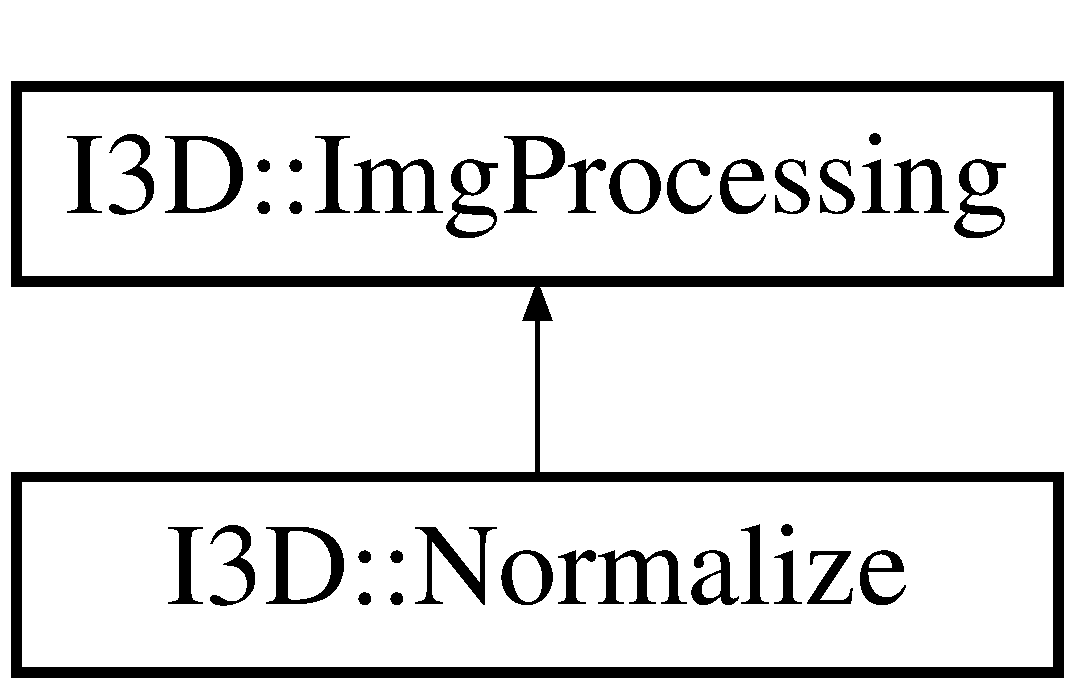
\includegraphics[height=2.000000cm]{class_i3_d_1_1_normalize}
\end{center}
\end{figure}
\subsection*{Métodos públicos}
\begin{DoxyCompactItemize}
\item 
\hyperlink{class_i3_d_1_1_normalize_abeae8c0f45fc949785ebf3e23f0de549}{Normalize} (double low\+Range, double up\+Range)
\begin{DoxyCompactList}\small\item\em Constructora de la clase \hyperlink{class_i3_d_1_1_normalize}{Normalize}. \end{DoxyCompactList}\item 
int \hyperlink{class_i3_d_1_1_normalize_a14506e377bd5da73c37ce960c2fdf07e}{execute} (const cv\+::\+Mat \&mat\+In, cv\+::\+Mat $\ast$mat\+Out) const  override
\begin{DoxyCompactList}\small\item\em Ejecuta el proceso. \end{DoxyCompactList}\item 
void \hyperlink{class_i3_d_1_1_normalize_a58456ec9333d041e0a86c9f03dec92da}{set\+Parameters} (double low\+Range, double up\+Range)
\begin{DoxyCompactList}\small\item\em Establece los parámetros. \end{DoxyCompactList}\end{DoxyCompactItemize}
\subsection*{Otros miembros heredados}


\subsection{Descripción detallada}
Clase \hyperlink{class_i3_d_1_1_normalize}{Normalize}. 

\subsection{Documentación del constructor y destructor}
\index{I3\+D\+::\+Normalize@{I3\+D\+::\+Normalize}!Normalize@{Normalize}}
\index{Normalize@{Normalize}!I3\+D\+::\+Normalize@{I3\+D\+::\+Normalize}}
\subsubsection[{\texorpdfstring{Normalize(double low\+Range, double up\+Range)}{Normalize(double lowRange, double upRange)}}]{\setlength{\rightskip}{0pt plus 5cm}I3\+D\+::\+Normalize\+::\+Normalize (
\begin{DoxyParamCaption}
\item[{double}]{low\+Range, }
\item[{double}]{up\+Range}
\end{DoxyParamCaption}
)\hspace{0.3cm}{\ttfamily [inline]}}\hypertarget{class_i3_d_1_1_normalize_abeae8c0f45fc949785ebf3e23f0de549}{}\label{class_i3_d_1_1_normalize_abeae8c0f45fc949785ebf3e23f0de549}


Constructora de la clase \hyperlink{class_i3_d_1_1_normalize}{Normalize}. 


\begin{DoxyParams}{Parámetros}
{\em low\+Range} & \\
\hline
{\em up\+Range} & \\
\hline
\end{DoxyParams}


\subsection{Documentación de las funciones miembro}
\index{I3\+D\+::\+Normalize@{I3\+D\+::\+Normalize}!execute@{execute}}
\index{execute@{execute}!I3\+D\+::\+Normalize@{I3\+D\+::\+Normalize}}
\subsubsection[{\texorpdfstring{execute(const cv\+::\+Mat \&mat\+In, cv\+::\+Mat $\ast$mat\+Out) const  override}{execute(const cv::Mat &matIn, cv::Mat *matOut) const  override}}]{\setlength{\rightskip}{0pt plus 5cm}int I3\+D\+::\+Normalize\+::execute (
\begin{DoxyParamCaption}
\item[{const cv\+::\+Mat \&}]{mat\+In, }
\item[{cv\+::\+Mat $\ast$}]{mat\+Out}
\end{DoxyParamCaption}
) const\hspace{0.3cm}{\ttfamily [override]}, {\ttfamily [virtual]}}\hypertarget{class_i3_d_1_1_normalize_a14506e377bd5da73c37ce960c2fdf07e}{}\label{class_i3_d_1_1_normalize_a14506e377bd5da73c37ce960c2fdf07e}


Ejecuta el proceso. 


\begin{DoxyParams}[1]{Parámetros}
\mbox{\tt in}  & {\em mat\+In} & Imagen de entrada \\
\hline
\mbox{\tt out}  & {\em mat\+Out} & Imagen de salida \\
\hline
\end{DoxyParams}
\begin{DoxyReturn}{Devuelve}
Error. Si los procesos se ejecutan correctamente devuelve 0. 
\end{DoxyReturn}


Implementa \hyperlink{class_i3_d_1_1_img_processing_a74195f05bbf034566e9ff6e10f3af4c9}{I3\+D\+::\+Img\+Processing}.

\index{I3\+D\+::\+Normalize@{I3\+D\+::\+Normalize}!set\+Parameters@{set\+Parameters}}
\index{set\+Parameters@{set\+Parameters}!I3\+D\+::\+Normalize@{I3\+D\+::\+Normalize}}
\subsubsection[{\texorpdfstring{set\+Parameters(double low\+Range, double up\+Range)}{setParameters(double lowRange, double upRange)}}]{\setlength{\rightskip}{0pt plus 5cm}void I3\+D\+::\+Normalize\+::set\+Parameters (
\begin{DoxyParamCaption}
\item[{double}]{low\+Range, }
\item[{double}]{up\+Range}
\end{DoxyParamCaption}
)}\hypertarget{class_i3_d_1_1_normalize_a58456ec9333d041e0a86c9f03dec92da}{}\label{class_i3_d_1_1_normalize_a58456ec9333d041e0a86c9f03dec92da}


Establece los parámetros. 


\begin{DoxyParams}[1]{Parámetros}
\mbox{\tt in}  & {\em low\+Range} & Rango inferior \\
\hline
\mbox{\tt in}  & {\em up\+Range} & Rango superior \\
\hline
\end{DoxyParams}


La documentación para esta clase fue generada a partir de los siguientes ficheros\+:\begin{DoxyCompactItemize}
\item 
D\+:/\+Desarrollo/tidop/src/\hyperlink{_img_processing_8h}{Img\+Processing.\+h}\item 
D\+:/\+Desarrollo/tidop/src/\hyperlink{_img_processing_8cpp}{Img\+Processing.\+cpp}\end{DoxyCompactItemize}

\hypertarget{class_i3_d_1_1_opening}{}\section{Referencia de la Clase I3D\+:\+:Opening}
\label{class_i3_d_1_1_opening}\index{I3\+D\+::\+Opening@{I3\+D\+::\+Opening}}


Operación morfológica de apertura Esta operación consite en aplicar una erosion de la imagen seguida de una dilatación.  




{\ttfamily \#include $<$Img\+Processing.\+h$>$}

Diagrama de herencias de I3D\+:\+:Opening\begin{figure}[H]
\begin{center}
\leavevmode
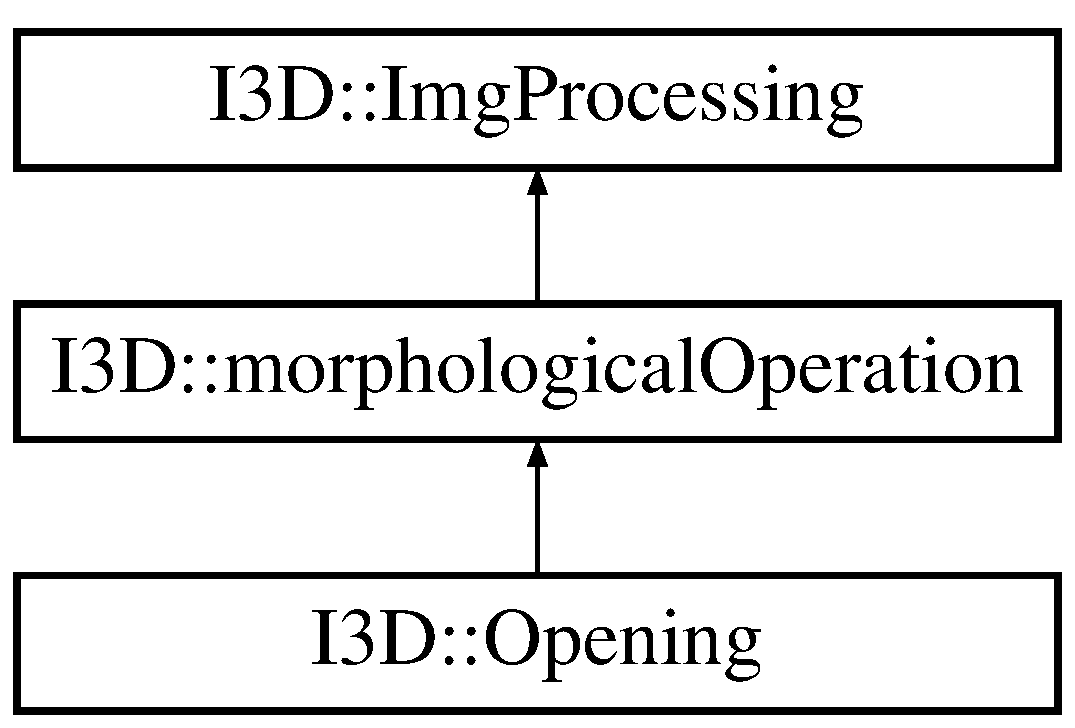
\includegraphics[height=3.000000cm]{class_i3_d_1_1_opening}
\end{center}
\end{figure}
\subsection*{Métodos públicos}
\begin{DoxyCompactItemize}
\item 
\hyperlink{class_i3_d_1_1_opening_aadbc4c4574ab7332a109d16deaee21bc}{Opening} (int size, cv\+::\+Morph\+Shapes shapes=cv\+::\+M\+O\+R\+P\+H\+\_\+\+R\+E\+CT, cv\+::\+Point anchor=cv\+::\+Point(-\/1,-\/1), int iterations=1, int border\+Type=cv\+::\+B\+O\+R\+D\+E\+R\+\_\+\+C\+O\+N\+S\+T\+A\+NT, const cv\+::\+Scalar \&border\+Value=cv\+::morphology\+Default\+Border\+Value())
\begin{DoxyCompactList}\small\item\em Constructora clase \hyperlink{class_i3_d_1_1_opening}{Opening}. \end{DoxyCompactList}\end{DoxyCompactItemize}
\subsection*{Otros miembros heredados}


\subsection{Descripción detallada}
Operación morfológica de apertura Esta operación consite en aplicar una erosion de la imagen seguida de una dilatación. 

\subsection{Documentación del constructor y destructor}
\index{I3\+D\+::\+Opening@{I3\+D\+::\+Opening}!Opening@{Opening}}
\index{Opening@{Opening}!I3\+D\+::\+Opening@{I3\+D\+::\+Opening}}
\subsubsection[{\texorpdfstring{Opening(int size, cv\+::\+Morph\+Shapes shapes=cv\+::\+M\+O\+R\+P\+H\+\_\+\+R\+E\+C\+T, cv\+::\+Point anchor=cv\+::\+Point(-\/1,-\/1), int iterations=1, int border\+Type=cv\+::\+B\+O\+R\+D\+E\+R\+\_\+\+C\+O\+N\+S\+T\+A\+N\+T, const cv\+::\+Scalar \&border\+Value=cv\+::morphology\+Default\+Border\+Value())}{Opening(int size, cv::MorphShapes shapes=cv::MORPH_RECT, cv::Point anchor=cv::Point(-1,-1), int iterations=1, int borderType=cv::BORDER_CONSTANT, const cv::Scalar &borderValue=cv::morphologyDefaultBorderValue())}}]{\setlength{\rightskip}{0pt plus 5cm}I3\+D\+::\+Opening\+::\+Opening (
\begin{DoxyParamCaption}
\item[{int}]{size, }
\item[{cv\+::\+Morph\+Shapes}]{shapes = {\ttfamily cv\+:\+:MORPH\+\_\+RECT}, }
\item[{cv\+::\+Point}]{anchor = {\ttfamily cv\+:\+:Point(-\/1,~-\/1)}, }
\item[{int}]{iterations = {\ttfamily 1}, }
\item[{int}]{border\+Type = {\ttfamily cv\+:\+:BORDER\+\_\+CONSTANT}, }
\item[{const cv\+::\+Scalar \&}]{border\+Value = {\ttfamily cv\+:\+:morphologyDefaultBorderValue()}}
\end{DoxyParamCaption}
)\hspace{0.3cm}{\ttfamily [inline]}}\hypertarget{class_i3_d_1_1_opening_aadbc4c4574ab7332a109d16deaee21bc}{}\label{class_i3_d_1_1_opening_aadbc4c4574ab7332a109d16deaee21bc}


Constructora clase \hyperlink{class_i3_d_1_1_opening}{Opening}. 


\begin{DoxyParams}[1]{Parámetros}
\mbox{\tt in}  & {\em size} & \\
\hline
\mbox{\tt in}  & {\em type} & \\
\hline
\mbox{\tt in}  & {\em anchor} & Punto de anclaje. Por defecto es el centro del kernel \\
\hline
\mbox{\tt in}  & {\em iterations} & \\
\hline
\mbox{\tt in}  & {\em border\+Type} & Método de extrapolación \\
\hline
\mbox{\tt in}  & {\em border\+Value} & \\
\hline
\end{DoxyParams}


La documentación para esta clase fue generada a partir del siguiente fichero\+:\begin{DoxyCompactItemize}
\item 
D\+:/\+Desarrollo/tidop/src/\hyperlink{_img_processing_8h}{Img\+Processing.\+h}\end{DoxyCompactItemize}

\hypertarget{class_i3_d_1_1_projective}{}\section{Referencia de la plantilla de la Clase I3D\+:\+:Projective$<$ T $>$}
\label{class_i3_d_1_1_projective}\index{I3\+D\+::\+Projective$<$ T $>$@{I3\+D\+::\+Projective$<$ T $>$}}


Transformación Projectiva.  




{\ttfamily \#include $<$transform.\+h$>$}

Diagrama de herencias de I3D\+:\+:Projective$<$ T $>$\begin{figure}[H]
\begin{center}
\leavevmode
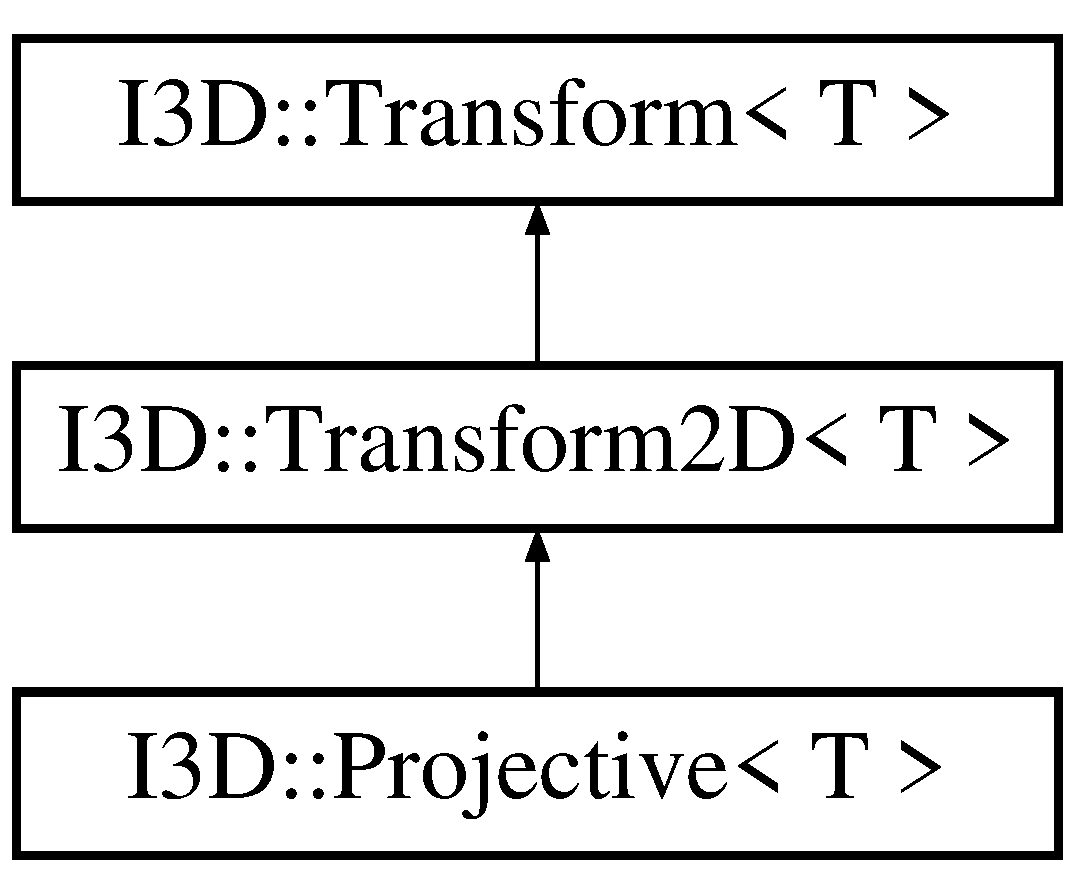
\includegraphics[height=3.000000cm]{class_i3_d_1_1_projective}
\end{center}
\end{figure}
\subsection*{Métodos públicos}
\begin{DoxyCompactItemize}
\item 
\hyperlink{class_i3_d_1_1_projective_a0557393a26c7c3324be20d7c481ca323}{Projective} ()
\begin{DoxyCompactList}\small\item\em Constructor por defecto. \end{DoxyCompactList}\item 
\hyperlink{class_i3_d_1_1_projective_ae355c6c6aa3825bc3e808a25166724c3}{Projective} (double a, double b, double c, double d, double e, double f, double g, double h)
\begin{DoxyCompactList}\small\item\em Constructor. \end{DoxyCompactList}\item 
bool \hyperlink{group__trf2_d_group_gaae888e9e90db1050898b63386252fc88}{compute} (const std\+::vector$<$ T $>$ \&pts1, const std\+::vector$<$ T $>$ \&pts2) override
\begin{DoxyCompactList}\small\item\em Calcula la transformación Helmert 2D entre dos sistemas diferentes a partir de dos conjuntos de puntos en cada sistema. \end{DoxyCompactList}\item 
void \hyperlink{group__trf2_d_group_ga9339dfc7f978fa6bbb9e2233930e8a3c}{transform} (const std\+::vector$<$ T $>$ \&in, std\+::vector$<$ T $>$ $\ast$out, bool b\+Direct=true) const  override
\begin{DoxyCompactList}\small\item\em Transforma un conjunto de puntos en otro aplicando un helmert 2D. \end{DoxyCompactList}\item 
void \hyperlink{group__trf2_d_group_ga1ecc0ebf8cc05c94bd9d9033416ac358}{transform} (const T \&in, T $\ast$out, bool b\+Direct=true) const 
\begin{DoxyCompactList}\small\item\em Aplica un helmert 2D a un punto. \end{DoxyCompactList}\item 
T \hyperlink{group__trf2_d_group_gaf5ad47e08dc23464413870c2b7da4fc0}{transform} (const T \&in, bool b\+Direct=true) const 
\begin{DoxyCompactList}\small\item\em Aplica un helmert 2D a un punto. \end{DoxyCompactList}\item 
void \hyperlink{group__trf2_d_group_gaf03861962a0be948aaa7e032b9e1729b}{set\+Parameters} (double a, double b, double c, double d, double e, double f, double g, double h)
\begin{DoxyCompactList}\small\item\em Establece los parámetros. \end{DoxyCompactList}\end{DoxyCompactItemize}
\subsection*{Otros miembros heredados}


\subsection{Descripción detallada}
\subsubsection*{template$<$typename T$>$\\*
class I3\+D\+::\+Projective$<$ T $>$}

Transformación Projectiva. 

La Transformación Projectiva expresa la relación que existe entre dos planos.

\begin{quote}
x\textquotesingle{} = ( a $\ast$ x + b $\ast$ y + c ) / ( g $\ast$ x + h $\ast$ y + 1 ) ~\newline
 y\textquotesingle{} = ( d $\ast$ x + e $\ast$ y + f ) / ( g $\ast$ x + h $\ast$ y + 1 ) \end{quote}


\subsection{Documentación del constructor y destructor}
\index{I3\+D\+::\+Projective@{I3\+D\+::\+Projective}!Projective@{Projective}}
\index{Projective@{Projective}!I3\+D\+::\+Projective@{I3\+D\+::\+Projective}}
\subsubsection[{\texorpdfstring{Projective()}{Projective()}}]{\setlength{\rightskip}{0pt plus 5cm}template$<$typename T $>$ {\bf I3\+D\+::\+Projective}$<$ T $>$\+::{\bf Projective} (
\begin{DoxyParamCaption}
{}
\end{DoxyParamCaption}
)\hspace{0.3cm}{\ttfamily [inline]}}\hypertarget{class_i3_d_1_1_projective_a0557393a26c7c3324be20d7c481ca323}{}\label{class_i3_d_1_1_projective_a0557393a26c7c3324be20d7c481ca323}


Constructor por defecto. 

\index{I3\+D\+::\+Projective@{I3\+D\+::\+Projective}!Projective@{Projective}}
\index{Projective@{Projective}!I3\+D\+::\+Projective@{I3\+D\+::\+Projective}}
\subsubsection[{\texorpdfstring{Projective(double a, double b, double c, double d, double e, double f, double g, double h)}{Projective(double a, double b, double c, double d, double e, double f, double g, double h)}}]{\setlength{\rightskip}{0pt plus 5cm}template$<$typename T $>$ {\bf I3\+D\+::\+Projective}$<$ T $>$\+::{\bf Projective} (
\begin{DoxyParamCaption}
\item[{double}]{a, }
\item[{double}]{b, }
\item[{double}]{c, }
\item[{double}]{d, }
\item[{double}]{e, }
\item[{double}]{f, }
\item[{double}]{g, }
\item[{double}]{h}
\end{DoxyParamCaption}
)\hspace{0.3cm}{\ttfamily [inline]}}\hypertarget{class_i3_d_1_1_projective_ae355c6c6aa3825bc3e808a25166724c3}{}\label{class_i3_d_1_1_projective_ae355c6c6aa3825bc3e808a25166724c3}


Constructor. 


\begin{DoxyParams}[1]{Parámetros}
\mbox{\tt in}  & {\em a} & \\
\hline
\mbox{\tt in}  & {\em b} & \\
\hline
\mbox{\tt in}  & {\em c} & \\
\hline
\mbox{\tt in}  & {\em d} & \\
\hline
\mbox{\tt in}  & {\em e} & \\
\hline
\mbox{\tt in}  & {\em f} & \\
\hline
\mbox{\tt in}  & {\em g} & \\
\hline
\mbox{\tt in}  & {\em h} & \\
\hline
\end{DoxyParams}


La documentación para esta clase fue generada a partir del siguiente fichero\+:\begin{DoxyCompactItemize}
\item 
C\+:/\+Desarrollo/tidop/src/\hyperlink{transform_8h}{transform.\+h}\end{DoxyCompactItemize}

\hypertarget{class_i3_d_1_1_resize}{}\section{Referencia de la Clase I3D\+:\+:Resize}
\label{class_i3_d_1_1_resize}\index{I3\+D\+::\+Resize@{I3\+D\+::\+Resize}}


The \hyperlink{class_i3_d_1_1_resize}{Resize} class.  




{\ttfamily \#include $<$Img\+Processing.\+h$>$}

Diagrama de herencias de I3D\+:\+:Resize\begin{figure}[H]
\begin{center}
\leavevmode
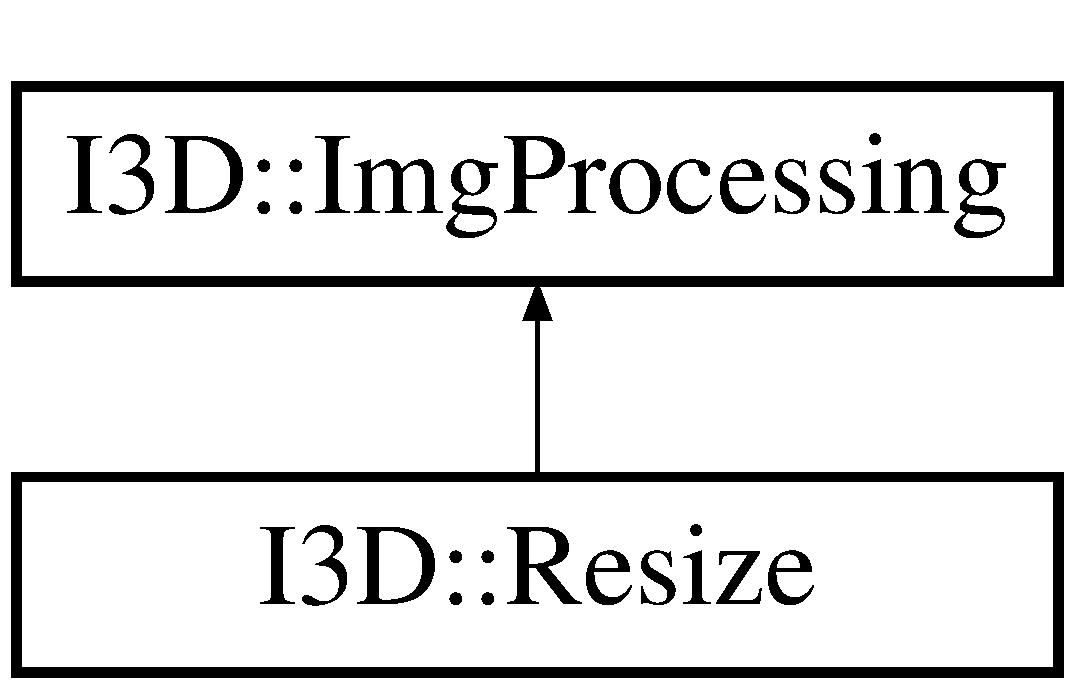
\includegraphics[height=2.000000cm]{class_i3_d_1_1_resize}
\end{center}
\end{figure}
\subsection*{Métodos públicos}
\begin{DoxyCompactItemize}
\item 
\hyperlink{class_i3_d_1_1_resize_a4f0bbaa5ea82c7390880dae533a34a92}{Resize} (int width, int height)
\begin{DoxyCompactList}\small\item\em Constructora. \end{DoxyCompactList}\item 
int \hyperlink{class_i3_d_1_1_resize_a683bd71d9e24c64416dc68231728a73e}{execute} (const cv\+::\+Mat \&mat\+In, cv\+::\+Mat $\ast$mat\+Out) const  override
\begin{DoxyCompactList}\small\item\em Ejecuta el proceso. \end{DoxyCompactList}\item 
void \hyperlink{class_i3_d_1_1_resize_adbe9397a26987a2744c509ad1e08d6f5}{set\+Parameters} (int width, int height)
\begin{DoxyCompactList}\small\item\em Establece los parámetros. \end{DoxyCompactList}\end{DoxyCompactItemize}
\subsection*{Otros miembros heredados}


\subsection{Descripción detallada}
The \hyperlink{class_i3_d_1_1_resize}{Resize} class. 

\subsection{Documentación del constructor y destructor}
\index{I3\+D\+::\+Resize@{I3\+D\+::\+Resize}!Resize@{Resize}}
\index{Resize@{Resize}!I3\+D\+::\+Resize@{I3\+D\+::\+Resize}}
\subsubsection[{\texorpdfstring{Resize(int width, int height)}{Resize(int width, int height)}}]{\setlength{\rightskip}{0pt plus 5cm}I3\+D\+::\+Resize\+::\+Resize (
\begin{DoxyParamCaption}
\item[{int}]{width, }
\item[{int}]{height}
\end{DoxyParamCaption}
)\hspace{0.3cm}{\ttfamily [inline]}}\hypertarget{class_i3_d_1_1_resize_a4f0bbaa5ea82c7390880dae533a34a92}{}\label{class_i3_d_1_1_resize_a4f0bbaa5ea82c7390880dae533a34a92}


Constructora. 


\begin{DoxyParams}[1]{Parámetros}
\mbox{\tt in}  & {\em width} & \\
\hline
\mbox{\tt in}  & {\em height} & \\
\hline
\end{DoxyParams}


\subsection{Documentación de las funciones miembro}
\index{I3\+D\+::\+Resize@{I3\+D\+::\+Resize}!execute@{execute}}
\index{execute@{execute}!I3\+D\+::\+Resize@{I3\+D\+::\+Resize}}
\subsubsection[{\texorpdfstring{execute(const cv\+::\+Mat \&mat\+In, cv\+::\+Mat $\ast$mat\+Out) const  override}{execute(const cv::Mat &matIn, cv::Mat *matOut) const  override}}]{\setlength{\rightskip}{0pt plus 5cm}int I3\+D\+::\+Resize\+::execute (
\begin{DoxyParamCaption}
\item[{const cv\+::\+Mat \&}]{mat\+In, }
\item[{cv\+::\+Mat $\ast$}]{mat\+Out}
\end{DoxyParamCaption}
) const\hspace{0.3cm}{\ttfamily [override]}, {\ttfamily [virtual]}}\hypertarget{class_i3_d_1_1_resize_a683bd71d9e24c64416dc68231728a73e}{}\label{class_i3_d_1_1_resize_a683bd71d9e24c64416dc68231728a73e}


Ejecuta el proceso. 


\begin{DoxyParams}[1]{Parámetros}
\mbox{\tt in}  & {\em mat\+In} & Imagen de entrada. \\
\hline
\mbox{\tt out}  & {\em mat\+Out} & Imagen de salida. \\
\hline
\end{DoxyParams}
\begin{DoxyReturn}{Devuelve}
Error. Si los procesos se ejecutan correctamente devuelve 0. 
\end{DoxyReturn}


Implementa \hyperlink{class_i3_d_1_1_img_processing_a74195f05bbf034566e9ff6e10f3af4c9}{I3\+D\+::\+Img\+Processing}.

\index{I3\+D\+::\+Resize@{I3\+D\+::\+Resize}!set\+Parameters@{set\+Parameters}}
\index{set\+Parameters@{set\+Parameters}!I3\+D\+::\+Resize@{I3\+D\+::\+Resize}}
\subsubsection[{\texorpdfstring{set\+Parameters(int width, int height)}{setParameters(int width, int height)}}]{\setlength{\rightskip}{0pt plus 5cm}void I3\+D\+::\+Resize\+::set\+Parameters (
\begin{DoxyParamCaption}
\item[{int}]{width, }
\item[{int}]{height}
\end{DoxyParamCaption}
)}\hypertarget{class_i3_d_1_1_resize_adbe9397a26987a2744c509ad1e08d6f5}{}\label{class_i3_d_1_1_resize_adbe9397a26987a2744c509ad1e08d6f5}


Establece los parámetros. 


\begin{DoxyParams}[1]{Parámetros}
\mbox{\tt in}  & {\em width} & Ancho. \\
\hline
\mbox{\tt in}  & {\em height} & Alto. \\
\hline
\end{DoxyParams}


La documentación para esta clase fue generada a partir de los siguientes ficheros\+:\begin{DoxyCompactItemize}
\item 
C\+:/\+Desarrollo/tidop/src/\hyperlink{_img_processing_8h}{Img\+Processing.\+h}\item 
C\+:/\+Desarrollo/tidop/src/\hyperlink{_img_processing_8cpp}{Img\+Processing.\+cpp}\end{DoxyCompactItemize}

\hypertarget{class_i3_d_1_1_rotation}{}\section{Referencia de la plantilla de la Clase I3D\+:\+:Rotation$<$ T $>$}
\label{class_i3_d_1_1_rotation}\index{I3\+D\+::\+Rotation$<$ T $>$@{I3\+D\+::\+Rotation$<$ T $>$}}


Rotación.  




{\ttfamily \#include $<$transform.\+h$>$}

Diagrama de herencias de I3D\+:\+:Rotation$<$ T $>$\begin{figure}[H]
\begin{center}
\leavevmode
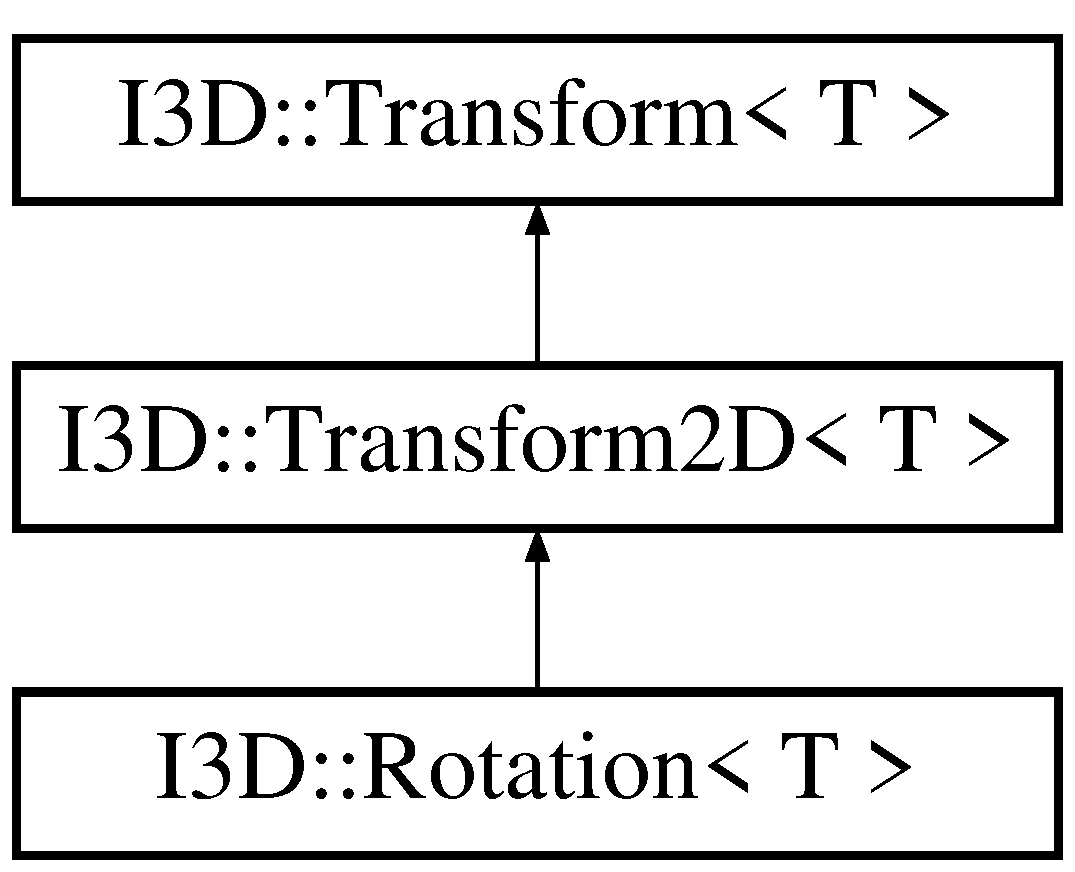
\includegraphics[height=3.000000cm]{class_i3_d_1_1_rotation}
\end{center}
\end{figure}
\subsection*{Métodos públicos}
\begin{DoxyCompactItemize}
\item 
\hyperlink{class_i3_d_1_1_rotation_aa256156103083742ff0b09e274302a02}{Rotation} ()
\begin{DoxyCompactList}\small\item\em Constructora por defecto. \end{DoxyCompactList}\item 
\hyperlink{class_i3_d_1_1_rotation_a76e534145c6f6c81b3d519d97b3d9353}{Rotation} (double angle)
\begin{DoxyCompactList}\small\item\em Constructora. \end{DoxyCompactList}\item 
bool \hyperlink{group__trf2_d_group_gae7637f88523deb1879cf8a712820d12e}{compute} (const std\+::vector$<$ T $>$ \&pts1, const std\+::vector$<$ T $>$ \&pts2) override
\begin{DoxyCompactList}\small\item\em Calculo del águlo de rotación. \end{DoxyCompactList}\item 
\hyperlink{class_i3_d_1_1_transform_ac087b4b8b9acb1b11a6caa2231d598c7}{sub\+\_\+type} \hyperlink{class_i3_d_1_1_rotation_ae7c5193c2f47f782b8707fd8cc02078f}{get\+Angle} () const 
\begin{DoxyCompactList}\small\item\em Devuelve el ángulo de la rotación. \end{DoxyCompactList}\item 
void \hyperlink{group__trf2_d_group_gacc531b7f0f00dd34f197a5c9ba07b8e2}{set\+Angle} (\hyperlink{class_i3_d_1_1_transform_ac087b4b8b9acb1b11a6caa2231d598c7}{sub\+\_\+type} ang)
\begin{DoxyCompactList}\small\item\em Establece en ángulo de la rotación. \end{DoxyCompactList}\item 
void \hyperlink{group__trf2_d_group_ga0032788395928aa7419d506981ef03d3}{transform} (const std\+::vector$<$ T $>$ \&in, std\+::vector$<$ T $>$ $\ast$out, bool b\+Direct=true) const  override
\begin{DoxyCompactList}\small\item\em Aplica una rotación a un conjunto de puntos. \end{DoxyCompactList}\item 
void \hyperlink{group__trf2_d_group_ga40ad8baf1f908752fe8afe20b71e8d67}{transform} (const T \&in, T $\ast$out, bool b\+Direct=true) const 
\begin{DoxyCompactList}\small\item\em Aplica una rotación a un punto. \end{DoxyCompactList}\item 
T \hyperlink{group__trf2_d_group_ga7db02aea0ee3a8c5167e16de0c89b079}{transform} (const T \&in, bool b\+Direct=true) const 
\begin{DoxyCompactList}\small\item\em Aplica una rotación a un punto. \end{DoxyCompactList}\end{DoxyCompactItemize}
\subsection*{Otros miembros heredados}


\subsection{Descripción detallada}
\subsubsection*{template$<$typename T$>$\\*
class I3\+D\+::\+Rotation$<$ T $>$}

Rotación. 

Transformación que aplica una rotación en el plano a un conjunto de puntos 

\subsection{Documentación del constructor y destructor}
\index{I3\+D\+::\+Rotation@{I3\+D\+::\+Rotation}!Rotation@{Rotation}}
\index{Rotation@{Rotation}!I3\+D\+::\+Rotation@{I3\+D\+::\+Rotation}}
\subsubsection[{\texorpdfstring{Rotation()}{Rotation()}}]{\setlength{\rightskip}{0pt plus 5cm}template$<$typename T $>$ {\bf I3\+D\+::\+Rotation}$<$ T $>$\+::{\bf Rotation} (
\begin{DoxyParamCaption}
{}
\end{DoxyParamCaption}
)\hspace{0.3cm}{\ttfamily [inline]}}\hypertarget{class_i3_d_1_1_rotation_aa256156103083742ff0b09e274302a02}{}\label{class_i3_d_1_1_rotation_aa256156103083742ff0b09e274302a02}


Constructora por defecto. 

\index{I3\+D\+::\+Rotation@{I3\+D\+::\+Rotation}!Rotation@{Rotation}}
\index{Rotation@{Rotation}!I3\+D\+::\+Rotation@{I3\+D\+::\+Rotation}}
\subsubsection[{\texorpdfstring{Rotation(double angle)}{Rotation(double angle)}}]{\setlength{\rightskip}{0pt plus 5cm}template$<$typename T $>$ {\bf I3\+D\+::\+Rotation}$<$ T $>$\+::{\bf Rotation} (
\begin{DoxyParamCaption}
\item[{double}]{angle}
\end{DoxyParamCaption}
)\hspace{0.3cm}{\ttfamily [inline]}}\hypertarget{class_i3_d_1_1_rotation_a76e534145c6f6c81b3d519d97b3d9353}{}\label{class_i3_d_1_1_rotation_a76e534145c6f6c81b3d519d97b3d9353}


Constructora. 


\begin{DoxyParams}[1]{Parámetros}
\mbox{\tt in}  & {\em angle} & Ángulo en radianes \\
\hline
\end{DoxyParams}


\subsection{Documentación de las funciones miembro}
\index{I3\+D\+::\+Rotation@{I3\+D\+::\+Rotation}!get\+Angle@{get\+Angle}}
\index{get\+Angle@{get\+Angle}!I3\+D\+::\+Rotation@{I3\+D\+::\+Rotation}}
\subsubsection[{\texorpdfstring{get\+Angle() const }{getAngle() const }}]{\setlength{\rightskip}{0pt plus 5cm}template$<$typename T $>$ {\bf sub\+\_\+type} {\bf I3\+D\+::\+Rotation}$<$ T $>$\+::get\+Angle (
\begin{DoxyParamCaption}
{}
\end{DoxyParamCaption}
) const\hspace{0.3cm}{\ttfamily [inline]}}\hypertarget{class_i3_d_1_1_rotation_ae7c5193c2f47f782b8707fd8cc02078f}{}\label{class_i3_d_1_1_rotation_ae7c5193c2f47f782b8707fd8cc02078f}


Devuelve el ángulo de la rotación. 

\begin{DoxyReturn}{Devuelve}
Ángulo en radianes 
\end{DoxyReturn}


La documentación para esta clase fue generada a partir del siguiente fichero\+:\begin{DoxyCompactItemize}
\item 
D\+:/\+Desarrollo/tidop/src/\hyperlink{transform_8h}{transform.\+h}\end{DoxyCompactItemize}

\hypertarget{class_i3_d_1_1_segment}{}\section{Referencia de la plantilla de la Clase I3D\+:\+:Segment$<$ T $>$}
\label{class_i3_d_1_1_segment}\index{I3\+D\+::\+Segment$<$ T $>$@{I3\+D\+::\+Segment$<$ T $>$}}


Clase segmento 2D.  




{\ttfamily \#include $<$segment.\+h$>$}

\subsection*{Tipos públicos}
\begin{DoxyCompactItemize}
\item 
typedef T \hyperlink{class_i3_d_1_1_segment_abc51866dd6396476534bda5afd87faf9}{type}
\begin{DoxyCompactList}\small\item\em type \end{DoxyCompactList}\end{DoxyCompactItemize}
\subsection*{Métodos públicos}
\begin{DoxyCompactItemize}
\item 
\hyperlink{group___geometric_entities_gac1c7a78862638e88bd9d9f512d6acc49}{Segment} ()
\begin{DoxyCompactList}\small\item\em Constructora por defecto. \end{DoxyCompactList}\item 
\hyperlink{group___geometric_entities_ga39a1c7ab363a4531d780dd35b6fc79f6}{Segment} (const \hyperlink{class_i3_d_1_1_segment}{Segment} \&segment)
\begin{DoxyCompactList}\small\item\em Constructor de copia. \end{DoxyCompactList}\item 
\hyperlink{group___geometric_entities_ga76e944eff092cf055965199957820f5b}{Segment} (const cv\+::\+Point\+\_\+$<$ T $>$ \&\+\_\+pt1, const cv\+::\+Point\+\_\+$<$ T $>$ \&\+\_\+pt2)
\begin{DoxyCompactList}\small\item\em Constructor segment. \end{DoxyCompactList}\item 
\hyperlink{group___geometric_entities_ga01623dcfd1be4e9472390b59e0ca3a58}{Segment} (const cv\+::\+Vec$<$ T, 4 $>$ \&lvect)
\begin{DoxyCompactList}\small\item\em Constructor segment. \end{DoxyCompactList}\item 
\hyperlink{class_i3_d_1_1_segment}{Segment} \& \hyperlink{group___geometric_entities_gad1b2c0a4c4e1ea3c43ee24630eb26f1b}{operator=} (const \hyperlink{class_i3_d_1_1_segment}{Segment} \&segment)
\begin{DoxyCompactList}\small\item\em Sobrecarga del operador de asignación. \end{DoxyCompactList}\item 
{\footnotesize template$<$typename T2 $>$ }\\\hyperlink{group___geometric_entities_ga363ef30b40d13ee361b9f0e32f135655}{operator Segment$<$ T2 $>$} () const 
\begin{DoxyCompactList}\small\item\em Conversión a un segmento de un tipo diferente. \end{DoxyCompactList}\item 
double \hyperlink{group___geometric_entities_ga911ebe69ce3cc5e6a486ef573d515866}{angle\+OX} () const 
\begin{DoxyCompactList}\small\item\em Angulo medido respecto al eje x. \end{DoxyCompactList}\item 
double \hyperlink{group___geometric_entities_ga324da1babfedb681fd7068fdc58d763b}{angle\+OY} () const 
\begin{DoxyCompactList}\small\item\em Angulo medido respecto al eje y. \end{DoxyCompactList}\item 
\hyperlink{class_i3_d_1_1_window}{Window}$<$ T $>$ \hyperlink{group___geometric_entities_ga3e11e0ecacba2003a023a21943693263}{get\+Window} () const 
\begin{DoxyCompactList}\small\item\em Ventana envolvente. \end{DoxyCompactList}\item 
bool \hyperlink{group___geometric_entities_ga59115064a0b57956175099eb3ff213ff}{is\+Near} (const \hyperlink{class_i3_d_1_1_segment}{Segment}$<$ T $>$ \&l2, double dist=10.) const 
\begin{DoxyCompactList}\small\item\em Comprueba si dos segmentos están próximos. \end{DoxyCompactList}\item 
bool \hyperlink{group___geometric_entities_ga7a4bcb31c98bdb2e239bdb64073e8874}{is\+Parallel} (const \hyperlink{class_i3_d_1_1_segment}{Segment}$<$ T $>$ \&l2, double tol=0.) const 
\begin{DoxyCompactList}\small\item\em Comprueba si es paralelo a otro segmento. \end{DoxyCompactList}\item 
double \hyperlink{class_i3_d_1_1_segment_a48dc929de83c7e1827e70e8fbf1c25c3}{length} () const 
\begin{DoxyCompactList}\small\item\em Longitud del segmento. \end{DoxyCompactList}\item 
cv\+::\+Point\+\_\+$<$ T $>$ \hyperlink{class_i3_d_1_1_segment_ae3d7380eae0db809d99d4ba81cba14ba}{vector} () const 
\begin{DoxyCompactList}\small\item\em Vector. \end{DoxyCompactList}\end{DoxyCompactItemize}
\subsection*{Atributos públicos}
\begin{DoxyCompactItemize}
\item 
cv\+::\+Point\+\_\+$<$ T $>$ \hyperlink{class_i3_d_1_1_segment_a5d431900fec31fe43607218ba4c382be}{pt1}
\begin{DoxyCompactList}\small\item\em Punto 1. \end{DoxyCompactList}\item 
cv\+::\+Point\+\_\+$<$ T $>$ \hyperlink{class_i3_d_1_1_segment_a15813aa4738a8e5ea4a06ad56fdb0e6d}{pt2}
\begin{DoxyCompactList}\small\item\em Punto 2. \end{DoxyCompactList}\end{DoxyCompactItemize}


\subsection{Descripción detallada}
\subsubsection*{template$<$typename T$>$\\*
class I3\+D\+::\+Segment$<$ T $>$}

Clase segmento 2D. 

Esta template representa un segmento recto entre dos puntos independientemente de que sean int, double o float. Se utiliza la clase point\+\_\+ de Open\+CV.

Se han definido los siguientes alias para facilitar el acceso\+: 
\begin{DoxyCode}
\textcolor{keyword}{typedef} Segment<int> \hyperlink{group___geometric_entities_ga929ca9aa27110ed7f1cf79c92664a6f0}{SegmentI};
\textcolor{keyword}{typedef} Segment<double> \hyperlink{group___geometric_entities_ga34bc194945585b7126a92e06c0571d5a}{SegmentD};
\textcolor{keyword}{typedef} Segment<float> \hyperlink{group___geometric_entities_gade7ab34fb1636ee6e5f7661bd0ae1937}{SegmentF};
\textcolor{keyword}{typedef} SegmentI \hyperlink{group___geometric_entities_ga483b43891a1b33d99406fdc397e9a445}{Line};
\end{DoxyCode}
 

\subsection{Documentación de los \textquotesingle{}Typedef\textquotesingle{} miembros de la clase}
\index{I3\+D\+::\+Segment@{I3\+D\+::\+Segment}!type@{type}}
\index{type@{type}!I3\+D\+::\+Segment@{I3\+D\+::\+Segment}}
\subsubsection[{\texorpdfstring{type}{type}}]{\setlength{\rightskip}{0pt plus 5cm}template$<$typename T$>$ typedef T {\bf I3\+D\+::\+Segment}$<$ T $>$\+::{\bf type}}\hypertarget{class_i3_d_1_1_segment_abc51866dd6396476534bda5afd87faf9}{}\label{class_i3_d_1_1_segment_abc51866dd6396476534bda5afd87faf9}


type 



\subsection{Documentación de las funciones miembro}
\index{I3\+D\+::\+Segment@{I3\+D\+::\+Segment}!length@{length}}
\index{length@{length}!I3\+D\+::\+Segment@{I3\+D\+::\+Segment}}
\subsubsection[{\texorpdfstring{length() const }{length() const }}]{\setlength{\rightskip}{0pt plus 5cm}template$<$typename T$>$ double {\bf I3\+D\+::\+Segment}$<$ T $>$\+::length (
\begin{DoxyParamCaption}
{}
\end{DoxyParamCaption}
) const\hspace{0.3cm}{\ttfamily [inline]}}\hypertarget{class_i3_d_1_1_segment_a48dc929de83c7e1827e70e8fbf1c25c3}{}\label{class_i3_d_1_1_segment_a48dc929de83c7e1827e70e8fbf1c25c3}


Longitud del segmento. 

\begin{DoxyReturn}{Devuelve}
Longitud del segmento 
\end{DoxyReturn}
\index{I3\+D\+::\+Segment@{I3\+D\+::\+Segment}!vector@{vector}}
\index{vector@{vector}!I3\+D\+::\+Segment@{I3\+D\+::\+Segment}}
\subsubsection[{\texorpdfstring{vector() const }{vector() const }}]{\setlength{\rightskip}{0pt plus 5cm}template$<$typename T$>$ cv\+::\+Point\+\_\+$<$T$>$ {\bf I3\+D\+::\+Segment}$<$ T $>$\+::vector (
\begin{DoxyParamCaption}
{}
\end{DoxyParamCaption}
) const\hspace{0.3cm}{\ttfamily [inline]}}\hypertarget{class_i3_d_1_1_segment_ae3d7380eae0db809d99d4ba81cba14ba}{}\label{class_i3_d_1_1_segment_ae3d7380eae0db809d99d4ba81cba14ba}


Vector. 

\begin{DoxyReturn}{Devuelve}
Vector del segmento 
\end{DoxyReturn}


\subsection{Documentación de los datos miembro}
\index{I3\+D\+::\+Segment@{I3\+D\+::\+Segment}!pt1@{pt1}}
\index{pt1@{pt1}!I3\+D\+::\+Segment@{I3\+D\+::\+Segment}}
\subsubsection[{\texorpdfstring{pt1}{pt1}}]{\setlength{\rightskip}{0pt plus 5cm}template$<$typename T$>$ cv\+::\+Point\+\_\+$<$T$>$ {\bf I3\+D\+::\+Segment}$<$ T $>$\+::pt1}\hypertarget{class_i3_d_1_1_segment_a5d431900fec31fe43607218ba4c382be}{}\label{class_i3_d_1_1_segment_a5d431900fec31fe43607218ba4c382be}


Punto 1. 

\index{I3\+D\+::\+Segment@{I3\+D\+::\+Segment}!pt2@{pt2}}
\index{pt2@{pt2}!I3\+D\+::\+Segment@{I3\+D\+::\+Segment}}
\subsubsection[{\texorpdfstring{pt2}{pt2}}]{\setlength{\rightskip}{0pt plus 5cm}template$<$typename T$>$ cv\+::\+Point\+\_\+$<$T$>$ {\bf I3\+D\+::\+Segment}$<$ T $>$\+::pt2}\hypertarget{class_i3_d_1_1_segment_a15813aa4738a8e5ea4a06ad56fdb0e6d}{}\label{class_i3_d_1_1_segment_a15813aa4738a8e5ea4a06ad56fdb0e6d}


Punto 2. 



La documentación para esta clase fue generada a partir del siguiente fichero\+:\begin{DoxyCompactItemize}
\item 
C\+:/\+Desarrollo/tidop/src/geometric\+\_\+entities/\hyperlink{segment_8h}{segment.\+h}\end{DoxyCompactItemize}

\hypertarget{class_i3_d_1_1_segment3_d}{}\section{Referencia de la plantilla de la Clase I3D\+:\+:Segment3D$<$ T $>$}
\label{class_i3_d_1_1_segment3_d}\index{I3\+D\+::\+Segment3\+D$<$ T $>$@{I3\+D\+::\+Segment3\+D$<$ T $>$}}


Clase segmento 3D.  




{\ttfamily \#include $<$segment.\+h$>$}

\subsection*{Tipos públicos}
\begin{DoxyCompactItemize}
\item 
typedef T \hyperlink{class_i3_d_1_1_segment3_d_a367ef41bf0a1e329a4363fe5e3731612}{type}
\end{DoxyCompactItemize}
\subsection*{Métodos públicos}
\begin{DoxyCompactItemize}
\item 
\hyperlink{group___geometric_entities_ga726c1cdb80b816445604fc035f0b709b}{Segment3D} ()
\begin{DoxyCompactList}\small\item\em Constructor por defecto. \end{DoxyCompactList}\item 
\hyperlink{group___geometric_entities_gad0a6b6c727b4f675429acb7a28518cbd}{Segment3D} (const \hyperlink{class_i3_d_1_1_segment3_d}{Segment3D} \&segment)
\begin{DoxyCompactList}\small\item\em Constructor de copia. \end{DoxyCompactList}\item 
\hyperlink{group___geometric_entities_ga7a2024be1820ddc19158004932d79882}{Segment3D} (const cv\+::\+Point3\+\_\+$<$ T $>$ \&\+\_\+pt1, const cv\+::\+Point3\+\_\+$<$ T $>$ \&\+\_\+pt2)
\begin{DoxyCompactList}\small\item\em Constructor segment. \end{DoxyCompactList}\item 
\hyperlink{class_i3_d_1_1_segment3_d}{Segment3D} \& \hyperlink{group___geometric_entities_gaa95bd137286b52bc178a569720bea3d6}{operator=} (const \hyperlink{class_i3_d_1_1_segment3_d}{Segment3D} \&segment)
\begin{DoxyCompactList}\small\item\em Sobrecarga del operador de asignación. \end{DoxyCompactList}\item 
{\footnotesize template$<$typename T2 $>$ }\\\hyperlink{group___geometric_entities_ga0a05ef1543e77df2c3dc9e40d2126b28}{operator Segment3\+D$<$ T2 $>$} () const 
\begin{DoxyCompactList}\small\item\em Conversión a un segmento de un tipo diferente. \end{DoxyCompactList}\item 
double \hyperlink{class_i3_d_1_1_segment3_d_a3194ca3e7b47dd389a460a7609ee4c1c}{length} () const 
\begin{DoxyCompactList}\small\item\em Longitud del segmento. \end{DoxyCompactList}\item 
cv\+::\+Point3\+\_\+$<$ T $>$ \hyperlink{class_i3_d_1_1_segment3_d_a4ac8bf44e4879682ee1626c5b74dbb3d}{vector} () const 
\begin{DoxyCompactList}\small\item\em Vector. \end{DoxyCompactList}\end{DoxyCompactItemize}
\subsection*{Atributos públicos}
\begin{DoxyCompactItemize}
\item 
cv\+::\+Point3\+\_\+$<$ T $>$ \hyperlink{class_i3_d_1_1_segment3_d_af9ee76f2e2b78d61ef8ea044bb47fe21}{pt1}
\begin{DoxyCompactList}\small\item\em Punto 1. \end{DoxyCompactList}\item 
cv\+::\+Point3\+\_\+$<$ T $>$ \hyperlink{class_i3_d_1_1_segment3_d_a91b9feb55271c1b1cbe6be0254904e21}{pt2}
\begin{DoxyCompactList}\small\item\em Punto 2. \end{DoxyCompactList}\end{DoxyCompactItemize}


\subsection{Descripción detallada}
\subsubsection*{template$<$typename T$>$\\*
class I3\+D\+::\+Segment3\+D$<$ T $>$}

Clase segmento 3D. 

Esta template representa un segmento recto entre dos puntos independientemente de que sean int, double o float. Se utiliza la clase Point3\+\_\+ de Open\+CV.

Se han definido los siguientes alias para facilitar el acceso\+:

typedef Segment3\+D$<$int$>$ Segment3dI; typedef Segment3\+D$<$double$>$ Segment3dD; typedef Segment3\+D$<$float$>$ Segment3dF; 

\subsection{Documentación de los \textquotesingle{}Typedef\textquotesingle{} miembros de la clase}
\index{I3\+D\+::\+Segment3D@{I3\+D\+::\+Segment3D}!type@{type}}
\index{type@{type}!I3\+D\+::\+Segment3D@{I3\+D\+::\+Segment3D}}
\subsubsection[{\texorpdfstring{type}{type}}]{\setlength{\rightskip}{0pt plus 5cm}template$<$typename T$>$ typedef T {\bf I3\+D\+::\+Segment3D}$<$ T $>$\+::{\bf type}}\hypertarget{class_i3_d_1_1_segment3_d_a367ef41bf0a1e329a4363fe5e3731612}{}\label{class_i3_d_1_1_segment3_d_a367ef41bf0a1e329a4363fe5e3731612}


\subsection{Documentación de las funciones miembro}
\index{I3\+D\+::\+Segment3D@{I3\+D\+::\+Segment3D}!length@{length}}
\index{length@{length}!I3\+D\+::\+Segment3D@{I3\+D\+::\+Segment3D}}
\subsubsection[{\texorpdfstring{length() const }{length() const }}]{\setlength{\rightskip}{0pt plus 5cm}template$<$typename T$>$ double {\bf I3\+D\+::\+Segment3D}$<$ T $>$\+::length (
\begin{DoxyParamCaption}
{}
\end{DoxyParamCaption}
) const\hspace{0.3cm}{\ttfamily [inline]}}\hypertarget{class_i3_d_1_1_segment3_d_a3194ca3e7b47dd389a460a7609ee4c1c}{}\label{class_i3_d_1_1_segment3_d_a3194ca3e7b47dd389a460a7609ee4c1c}


Longitud del segmento. 

\begin{DoxyReturn}{Devuelve}
Longitud del segmento 
\end{DoxyReturn}
\index{I3\+D\+::\+Segment3D@{I3\+D\+::\+Segment3D}!vector@{vector}}
\index{vector@{vector}!I3\+D\+::\+Segment3D@{I3\+D\+::\+Segment3D}}
\subsubsection[{\texorpdfstring{vector() const }{vector() const }}]{\setlength{\rightskip}{0pt plus 5cm}template$<$typename T$>$ cv\+::\+Point3\+\_\+$<$T$>$ {\bf I3\+D\+::\+Segment3D}$<$ T $>$\+::vector (
\begin{DoxyParamCaption}
{}
\end{DoxyParamCaption}
) const\hspace{0.3cm}{\ttfamily [inline]}}\hypertarget{class_i3_d_1_1_segment3_d_a4ac8bf44e4879682ee1626c5b74dbb3d}{}\label{class_i3_d_1_1_segment3_d_a4ac8bf44e4879682ee1626c5b74dbb3d}


Vector. 

\begin{DoxyReturn}{Devuelve}
Vector del segmento 
\end{DoxyReturn}


\subsection{Documentación de los datos miembro}
\index{I3\+D\+::\+Segment3D@{I3\+D\+::\+Segment3D}!pt1@{pt1}}
\index{pt1@{pt1}!I3\+D\+::\+Segment3D@{I3\+D\+::\+Segment3D}}
\subsubsection[{\texorpdfstring{pt1}{pt1}}]{\setlength{\rightskip}{0pt plus 5cm}template$<$typename T$>$ cv\+::\+Point3\+\_\+$<$T$>$ {\bf I3\+D\+::\+Segment3D}$<$ T $>$\+::pt1}\hypertarget{class_i3_d_1_1_segment3_d_af9ee76f2e2b78d61ef8ea044bb47fe21}{}\label{class_i3_d_1_1_segment3_d_af9ee76f2e2b78d61ef8ea044bb47fe21}


Punto 1. 

\index{I3\+D\+::\+Segment3D@{I3\+D\+::\+Segment3D}!pt2@{pt2}}
\index{pt2@{pt2}!I3\+D\+::\+Segment3D@{I3\+D\+::\+Segment3D}}
\subsubsection[{\texorpdfstring{pt2}{pt2}}]{\setlength{\rightskip}{0pt plus 5cm}template$<$typename T$>$ cv\+::\+Point3\+\_\+$<$T$>$ {\bf I3\+D\+::\+Segment3D}$<$ T $>$\+::pt2}\hypertarget{class_i3_d_1_1_segment3_d_a91b9feb55271c1b1cbe6be0254904e21}{}\label{class_i3_d_1_1_segment3_d_a91b9feb55271c1b1cbe6be0254904e21}


Punto 2. 



La documentación para esta clase fue generada a partir del siguiente fichero\+:\begin{DoxyCompactItemize}
\item 
C\+:/\+Desarrollo/tidop/src/geometric\+\_\+entities/\hyperlink{segment_8h}{segment.\+h}\end{DoxyCompactItemize}

\hypertarget{class_i3_d_1_1_sobel}{}\section{Referencia de la Clase I3D\+:\+:Sobel}
\label{class_i3_d_1_1_sobel}\index{I3\+D\+::\+Sobel@{I3\+D\+::\+Sobel}}


\hyperlink{class_i3_d_1_1_sobel}{Sobel}.  




{\ttfamily \#include $<$Img\+Processing.\+h$>$}

Diagrama de herencias de I3D\+:\+:Sobel\begin{figure}[H]
\begin{center}
\leavevmode
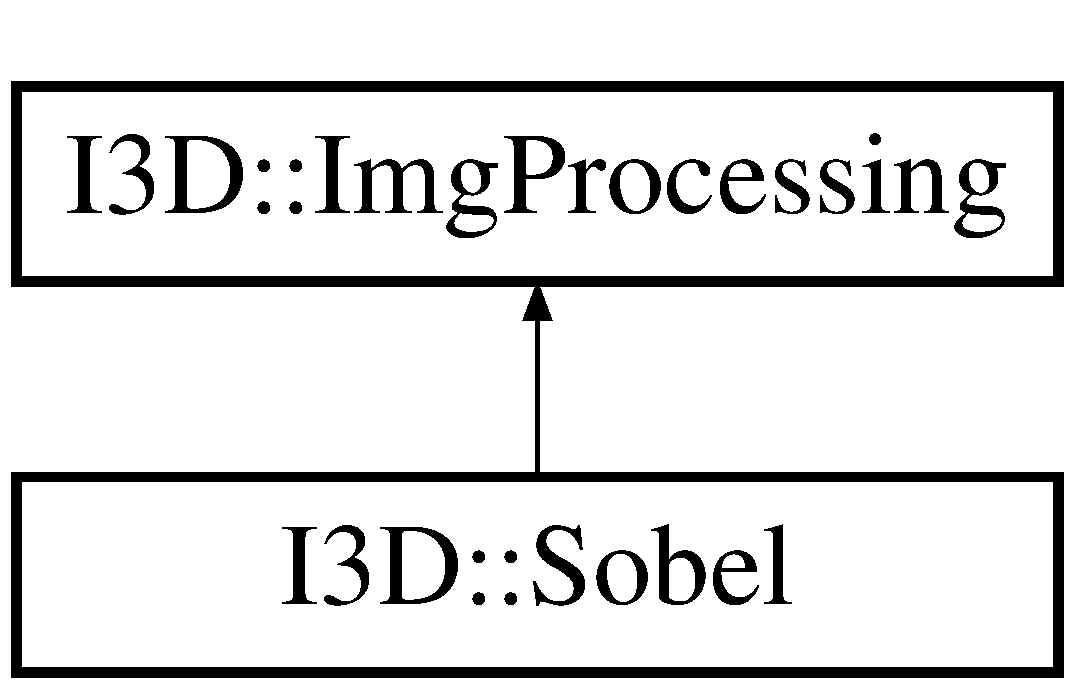
\includegraphics[height=2.000000cm]{class_i3_d_1_1_sobel}
\end{center}
\end{figure}
\subsection*{Métodos públicos}
\begin{DoxyCompactItemize}
\item 
\hyperlink{class_i3_d_1_1_sobel_a44bcc6981eb6875500cdee832174af71}{Sobel} (int dx, int dy, int ksize=3, double scale=1., double delta=0., int ddepth=C\+V\+\_\+16S, double thresh=50., double maxval=200., int bordertype=cv\+::\+B\+O\+R\+D\+E\+R\+\_\+\+D\+E\+F\+A\+U\+LT)
\begin{DoxyCompactList}\small\item\em Constructora. \end{DoxyCompactList}\item 
int \hyperlink{class_i3_d_1_1_sobel_a902c7392196e514597820fbe13a2a634}{execute} (const cv\+::\+Mat \&mat\+In, cv\+::\+Mat $\ast$mat\+Out) const  override
\begin{DoxyCompactList}\small\item\em Ejecuta el proceso. \end{DoxyCompactList}\item 
void \hyperlink{class_i3_d_1_1_sobel_a747c30a1d9b50aca3c7a6d737dc6c5c6}{set\+Parameters} (int dx, int dy, int ksize=3, double scale=1., double delta=0., int ddepth=C\+V\+\_\+16S, double thresh=50., double maxval=200., int bordertype=cv\+::\+B\+O\+R\+D\+E\+R\+\_\+\+D\+E\+F\+A\+U\+LT)
\begin{DoxyCompactList}\small\item\em Establece los parámetros. \end{DoxyCompactList}\end{DoxyCompactItemize}
\subsection*{Otros miembros heredados}


\subsection{Descripción detallada}
\hyperlink{class_i3_d_1_1_sobel}{Sobel}. 

\subsection{Documentación del constructor y destructor}
\index{I3\+D\+::\+Sobel@{I3\+D\+::\+Sobel}!Sobel@{Sobel}}
\index{Sobel@{Sobel}!I3\+D\+::\+Sobel@{I3\+D\+::\+Sobel}}
\subsubsection[{\texorpdfstring{Sobel(int dx, int dy, int ksize=3, double scale=1., double delta=0., int ddepth=\+C\+V\+\_\+16\+S, double thresh=50., double maxval=200., int bordertype=cv\+::\+B\+O\+R\+D\+E\+R\+\_\+\+D\+E\+F\+A\+U\+L\+T)}{Sobel(int dx, int dy, int ksize=3, double scale=1., double delta=0., int ddepth=CV_16S, double thresh=50., double maxval=200., int bordertype=cv::BORDER_DEFAULT)}}]{\setlength{\rightskip}{0pt plus 5cm}I3\+D\+::\+Sobel\+::\+Sobel (
\begin{DoxyParamCaption}
\item[{int}]{dx, }
\item[{int}]{dy, }
\item[{int}]{ksize = {\ttfamily 3}, }
\item[{double}]{scale = {\ttfamily 1.}, }
\item[{double}]{delta = {\ttfamily 0.}, }
\item[{int}]{ddepth = {\ttfamily CV\+\_\+16S}, }
\item[{double}]{thresh = {\ttfamily 50.}, }
\item[{double}]{maxval = {\ttfamily 200.}, }
\item[{int}]{bordertype = {\ttfamily cv\+:\+:BORDER\+\_\+DEFAULT}}
\end{DoxyParamCaption}
)\hspace{0.3cm}{\ttfamily [inline]}}\hypertarget{class_i3_d_1_1_sobel_a44bcc6981eb6875500cdee832174af71}{}\label{class_i3_d_1_1_sobel_a44bcc6981eb6875500cdee832174af71}


Constructora. 


\begin{DoxyParams}[1]{Parámetros}
\mbox{\tt in}  & {\em dx} & \\
\hline
\mbox{\tt in}  & {\em dy} & \\
\hline
\mbox{\tt in}  & {\em ksize} & \\
\hline
\mbox{\tt in}  & {\em scale} & \\
\hline
\mbox{\tt in}  & {\em delta} & \\
\hline
\mbox{\tt in}  & {\em ddepth} & \\
\hline
\mbox{\tt in}  & {\em thresh} & \\
\hline
\mbox{\tt in}  & {\em maxval} & \\
\hline
\mbox{\tt in}  & {\em bordertype} & \\
\hline
\end{DoxyParams}


\subsection{Documentación de las funciones miembro}
\index{I3\+D\+::\+Sobel@{I3\+D\+::\+Sobel}!execute@{execute}}
\index{execute@{execute}!I3\+D\+::\+Sobel@{I3\+D\+::\+Sobel}}
\subsubsection[{\texorpdfstring{execute(const cv\+::\+Mat \&mat\+In, cv\+::\+Mat $\ast$mat\+Out) const  override}{execute(const cv::Mat &matIn, cv::Mat *matOut) const  override}}]{\setlength{\rightskip}{0pt plus 5cm}int I3\+D\+::\+Sobel\+::execute (
\begin{DoxyParamCaption}
\item[{const cv\+::\+Mat \&}]{mat\+In, }
\item[{cv\+::\+Mat $\ast$}]{mat\+Out}
\end{DoxyParamCaption}
) const\hspace{0.3cm}{\ttfamily [override]}, {\ttfamily [virtual]}}\hypertarget{class_i3_d_1_1_sobel_a902c7392196e514597820fbe13a2a634}{}\label{class_i3_d_1_1_sobel_a902c7392196e514597820fbe13a2a634}


Ejecuta el proceso. 


\begin{DoxyParams}[1]{Parámetros}
\mbox{\tt in}  & {\em mat\+In} & Imagen de entrada \\
\hline
\mbox{\tt out}  & {\em mat\+Out} & Imagen de salida \\
\hline
\end{DoxyParams}
\begin{DoxyReturn}{Devuelve}
Error. Si los procesos se ejecutan correctamente devuelve 0. 
\end{DoxyReturn}


Implementa \hyperlink{class_i3_d_1_1_img_processing_a74195f05bbf034566e9ff6e10f3af4c9}{I3\+D\+::\+Img\+Processing}.

\index{I3\+D\+::\+Sobel@{I3\+D\+::\+Sobel}!set\+Parameters@{set\+Parameters}}
\index{set\+Parameters@{set\+Parameters}!I3\+D\+::\+Sobel@{I3\+D\+::\+Sobel}}
\subsubsection[{\texorpdfstring{set\+Parameters(int dx, int dy, int ksize=3, double scale=1., double delta=0., int ddepth=\+C\+V\+\_\+16\+S, double thresh=50., double maxval=200., int bordertype=cv\+::\+B\+O\+R\+D\+E\+R\+\_\+\+D\+E\+F\+A\+U\+L\+T)}{setParameters(int dx, int dy, int ksize=3, double scale=1., double delta=0., int ddepth=CV_16S, double thresh=50., double maxval=200., int bordertype=cv::BORDER_DEFAULT)}}]{\setlength{\rightskip}{0pt plus 5cm}void I3\+D\+::\+Sobel\+::set\+Parameters (
\begin{DoxyParamCaption}
\item[{int}]{dx, }
\item[{int}]{dy, }
\item[{int}]{ksize = {\ttfamily 3}, }
\item[{double}]{scale = {\ttfamily 1.}, }
\item[{double}]{delta = {\ttfamily 0.}, }
\item[{int}]{ddepth = {\ttfamily CV\+\_\+16S}, }
\item[{double}]{thresh = {\ttfamily 50.}, }
\item[{double}]{maxval = {\ttfamily 200.}, }
\item[{int}]{bordertype = {\ttfamily cv\+:\+:BORDER\+\_\+DEFAULT}}
\end{DoxyParamCaption}
)}\hypertarget{class_i3_d_1_1_sobel_a747c30a1d9b50aca3c7a6d737dc6c5c6}{}\label{class_i3_d_1_1_sobel_a747c30a1d9b50aca3c7a6d737dc6c5c6}


Establece los parámetros. 


\begin{DoxyParams}[1]{Parámetros}
\mbox{\tt in}  & {\em dx} & Orden de la derivada x \\
\hline
\mbox{\tt in}  & {\em dy} & Orden de la derivada y \\
\hline
\mbox{\tt in}  & {\em ksize} & Tamaño kernel \\
\hline
\mbox{\tt in}  & {\em scale} & Factor de escala opcional para los valores de las derivadas calculadas \\
\hline
\mbox{\tt in}  & {\em delta} & \\
\hline
\mbox{\tt in}  & {\em ddepth} & \\
\hline
\mbox{\tt in}  & {\em thresh} & \\
\hline
\mbox{\tt in}  & {\em maxval} & \\
\hline
\mbox{\tt in}  & {\em bordertype} & \\
\hline
\end{DoxyParams}


La documentación para esta clase fue generada a partir de los siguientes ficheros\+:\begin{DoxyCompactItemize}
\item 
C\+:/\+Desarrollo/tidop/src/\hyperlink{_img_processing_8h}{Img\+Processing.\+h}\item 
C\+:/\+Desarrollo/tidop/src/\hyperlink{_img_processing_8cpp}{Img\+Processing.\+cpp}\end{DoxyCompactItemize}

\hypertarget{class_i3_d_1_1_top_hat}{}\section{Referencia de la Clase I3D\+:\+:Top\+Hat}
\label{class_i3_d_1_1_top_hat}\index{I3\+D\+::\+Top\+Hat@{I3\+D\+::\+Top\+Hat}}


Operación morfológica Top Hat Es la diferencia entre una imagen y el resultado de aplicar una operación de apertura sobre la misma imagen.  




{\ttfamily \#include $<$Img\+Processing.\+h$>$}

Diagrama de herencias de I3D\+:\+:Top\+Hat\begin{figure}[H]
\begin{center}
\leavevmode
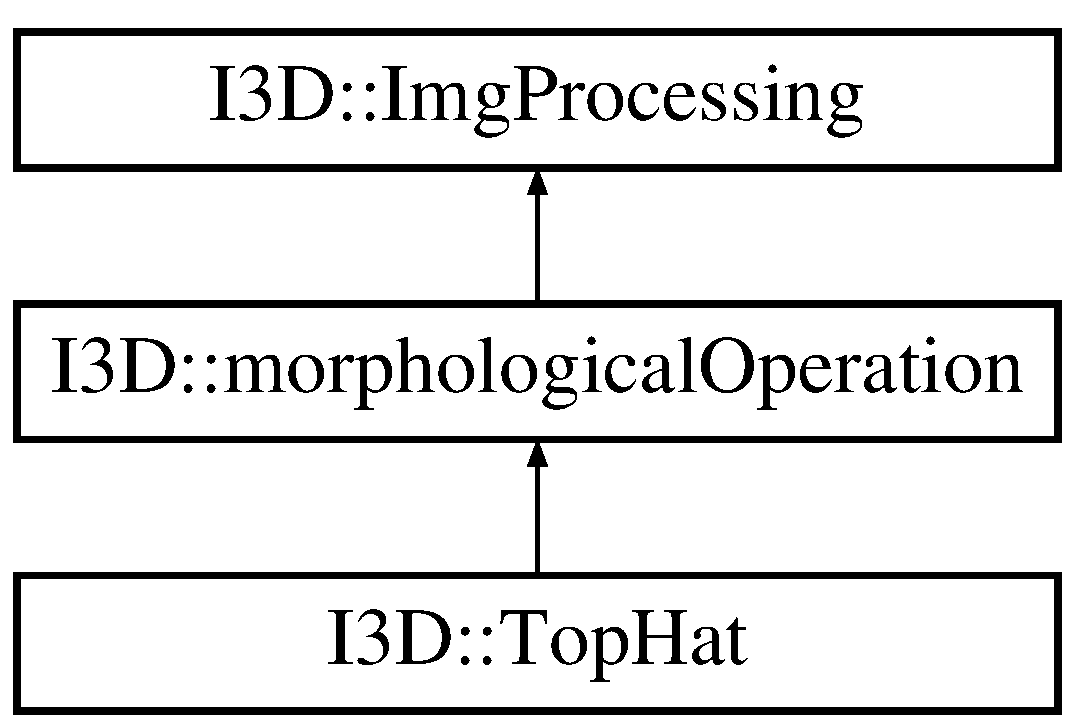
\includegraphics[height=3.000000cm]{class_i3_d_1_1_top_hat}
\end{center}
\end{figure}
\subsection*{Métodos públicos}
\begin{DoxyCompactItemize}
\item 
\hyperlink{class_i3_d_1_1_top_hat_a36e924a9ed4ea5ea850145c651b87671}{Top\+Hat} (int size, cv\+::\+Morph\+Shapes shapes=cv\+::\+M\+O\+R\+P\+H\+\_\+\+R\+E\+CT, cv\+::\+Point anchor=cv\+::\+Point(-\/1,-\/1), int iterations=1, int border\+Type=cv\+::\+B\+O\+R\+D\+E\+R\+\_\+\+C\+O\+N\+S\+T\+A\+NT, const cv\+::\+Scalar \&border\+Value=cv\+::morphology\+Default\+Border\+Value())
\begin{DoxyCompactList}\small\item\em Constructora clase \hyperlink{class_i3_d_1_1_closing}{Closing}. \end{DoxyCompactList}\end{DoxyCompactItemize}
\subsection*{Otros miembros heredados}


\subsection{Descripción detallada}
Operación morfológica Top Hat Es la diferencia entre una imagen y el resultado de aplicar una operación de apertura sobre la misma imagen. 

\subsection{Documentación del constructor y destructor}
\index{I3\+D\+::\+Top\+Hat@{I3\+D\+::\+Top\+Hat}!Top\+Hat@{Top\+Hat}}
\index{Top\+Hat@{Top\+Hat}!I3\+D\+::\+Top\+Hat@{I3\+D\+::\+Top\+Hat}}
\subsubsection[{\texorpdfstring{Top\+Hat(int size, cv\+::\+Morph\+Shapes shapes=cv\+::\+M\+O\+R\+P\+H\+\_\+\+R\+E\+C\+T, cv\+::\+Point anchor=cv\+::\+Point(-\/1,-\/1), int iterations=1, int border\+Type=cv\+::\+B\+O\+R\+D\+E\+R\+\_\+\+C\+O\+N\+S\+T\+A\+N\+T, const cv\+::\+Scalar \&border\+Value=cv\+::morphology\+Default\+Border\+Value())}{TopHat(int size, cv::MorphShapes shapes=cv::MORPH_RECT, cv::Point anchor=cv::Point(-1,-1), int iterations=1, int borderType=cv::BORDER_CONSTANT, const cv::Scalar &borderValue=cv::morphologyDefaultBorderValue())}}]{\setlength{\rightskip}{0pt plus 5cm}I3\+D\+::\+Top\+Hat\+::\+Top\+Hat (
\begin{DoxyParamCaption}
\item[{int}]{size, }
\item[{cv\+::\+Morph\+Shapes}]{shapes = {\ttfamily cv\+:\+:MORPH\+\_\+RECT}, }
\item[{cv\+::\+Point}]{anchor = {\ttfamily cv\+:\+:Point(-\/1,~-\/1)}, }
\item[{int}]{iterations = {\ttfamily 1}, }
\item[{int}]{border\+Type = {\ttfamily cv\+:\+:BORDER\+\_\+CONSTANT}, }
\item[{const cv\+::\+Scalar \&}]{border\+Value = {\ttfamily cv\+:\+:morphologyDefaultBorderValue()}}
\end{DoxyParamCaption}
)\hspace{0.3cm}{\ttfamily [inline]}}\hypertarget{class_i3_d_1_1_top_hat_a36e924a9ed4ea5ea850145c651b87671}{}\label{class_i3_d_1_1_top_hat_a36e924a9ed4ea5ea850145c651b87671}


Constructora clase \hyperlink{class_i3_d_1_1_closing}{Closing}. 


\begin{DoxyParams}[1]{Parámetros}
\mbox{\tt in}  & {\em size} & \\
\hline
\mbox{\tt in}  & {\em type} & \\
\hline
\mbox{\tt in}  & {\em anchor} & Punto de anclaje. Por defecto es el centro del kernel \\
\hline
\mbox{\tt in}  & {\em iterations} & \\
\hline
\mbox{\tt in}  & {\em border\+Type} & Método de extrapolación \\
\hline
\mbox{\tt in}  & {\em border\+Value} & \\
\hline
\end{DoxyParams}


La documentación para esta clase fue generada a partir del siguiente fichero\+:\begin{DoxyCompactItemize}
\item 
C\+:/\+Desarrollo/tidop/src/\hyperlink{_img_processing_8h}{Img\+Processing.\+h}\end{DoxyCompactItemize}

\hypertarget{class_i3_d_1_1_transform}{}\section{Referencia de la plantilla de la Clase I3D\+:\+:Transform$<$ T $>$}
\label{class_i3_d_1_1_transform}\index{I3\+D\+::\+Transform$<$ T $>$@{I3\+D\+::\+Transform$<$ T $>$}}


Clase base para transformaciones.  




{\ttfamily \#include $<$transform.\+h$>$}

Diagrama de herencias de I3D\+:\+:Transform$<$ T $>$\begin{figure}[H]
\begin{center}
\leavevmode
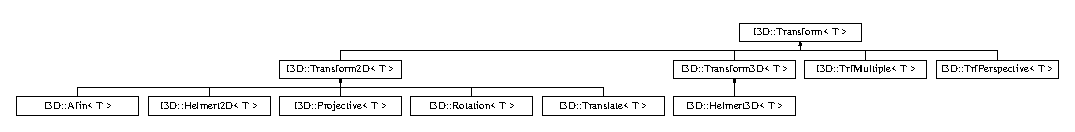
\includegraphics[height=1.320755cm]{class_i3_d_1_1_transform}
\end{center}
\end{figure}
\subsection*{Métodos públicos}
\begin{DoxyCompactItemize}
\item 
\hyperlink{class_i3_d_1_1_transform_a65f115efcbc52cec0dad27664e2e48c3}{Transform} (int n\+\_\+min=0, \hyperlink{group__trf_group_ga175e1580b1ecbc0710ad48060d56c2a3}{transform\+\_\+type} trf\+Type=\hyperlink{group__trf_group_gga175e1580b1ecbc0710ad48060d56c2a3a5b39c8b553c821e7cddc6da64b5bd2ee}{transform\+\_\+type\+::\+D\+E\+F\+A\+U\+LT})
\begin{DoxyCompactList}\small\item\em Constructor. \end{DoxyCompactList}\item 
virtual \hyperlink{class_i3_d_1_1_transform_a7b3aa01e8b48ee45604ebb9cc1e0ed56}{$\sim$\+Transform} ()
\begin{DoxyCompactList}\small\item\em Destructora. \end{DoxyCompactList}\item 
virtual bool \hyperlink{class_i3_d_1_1_transform_a909a4033f9fab3f091b433b9e2261208}{compute} (const std\+::vector$<$ T $>$ \&v1, const std\+::vector$<$ T $>$ \&v2)=0
\begin{DoxyCompactList}\small\item\em Calcula los parámetros de transformación. \end{DoxyCompactList}\item 
bool \hyperlink{class_i3_d_1_1_transform_ab02fc57452ec9edeb339242b682dc829}{is\+Number\+Of\+Points\+Valid} (int npoints) const 
\begin{DoxyCompactList}\small\item\em Determina si el numero de puntos son suficientes para calcular la transformación. \end{DoxyCompactList}\item 
virtual void \hyperlink{class_i3_d_1_1_transform_adbec7381bfc66b4a766a00fdf16de0fe}{transform} (const std\+::vector$<$ T $>$ \&in, std\+::vector$<$ T $>$ $\ast$out, bool b\+Direct=true) const  =0
\begin{DoxyCompactList}\small\item\em Aplica la transformación. \end{DoxyCompactList}\item 
int \hyperlink{class_i3_d_1_1_transform_ad0a61ba37895c3b70e47b9e66a69bbbd}{min\+Number\+Of\+Points} ()
\begin{DoxyCompactList}\small\item\em Número mínimo de puntos necesario para la transformación. \end{DoxyCompactList}\item 
\hyperlink{group__trf_group_ga175e1580b1ecbc0710ad48060d56c2a3}{transform\+\_\+type} \hyperlink{class_i3_d_1_1_transform_aaed30aa2e0b864a338c0bac5ccf3d963}{get\+Transform\+Type} ()
\begin{DoxyCompactList}\small\item\em Tipo de transformación. \end{DoxyCompactList}\end{DoxyCompactItemize}
\subsection*{Tipos protegidos}
\begin{DoxyCompactItemize}
\item 
typedef T\+::value\+\_\+type \hyperlink{class_i3_d_1_1_transform_ac087b4b8b9acb1b11a6caa2231d598c7}{sub\+\_\+type}
\end{DoxyCompactItemize}
\subsection*{Métodos protegidos}
\begin{DoxyCompactItemize}
\item 
{\footnotesize template$<$typename T2 $>$ }\\void \hyperlink{class_i3_d_1_1_transform_aa4d27a52571d16156699589050ffd7fc}{format\+Vector\+Out} (const std\+::vector$<$ T2 $>$ \&in, std\+::vector$<$ T2 $>$ $\ast$out) const 
\begin{DoxyCompactList}\small\item\em Formatea de forma adecuada el vector de salida. \end{DoxyCompactList}\end{DoxyCompactItemize}
\subsection*{Atributos protegidos}
\begin{DoxyCompactItemize}
\item 
\hyperlink{group__trf_group_ga175e1580b1ecbc0710ad48060d56c2a3}{transform\+\_\+type} \hyperlink{class_i3_d_1_1_transform_a1d5c0d6ea45417608b00316a08f164d7}{m\+Trf\+Type}
\begin{DoxyCompactList}\small\item\em Tipo de transformación. \end{DoxyCompactList}\item 
int \hyperlink{class_i3_d_1_1_transform_a087716ea2e7fa31127003e50479ed01e}{m\+Min\+Point}
\begin{DoxyCompactList}\small\item\em Número mínimo de puntos necesario para la transformación. \end{DoxyCompactList}\item 
int \hyperlink{class_i3_d_1_1_transform_a53fc627243795344379b92d0a48a31a9}{m\+Dimensions}
\end{DoxyCompactItemize}


\subsection{Descripción detallada}
\subsubsection*{template$<$typename T$>$\\*
class I3\+D\+::\+Transform$<$ T $>$}

Clase base para transformaciones. 

\subsection{Documentación de los \textquotesingle{}Typedef\textquotesingle{} miembros de la clase}
\index{I3\+D\+::\+Transform@{I3\+D\+::\+Transform}!sub\+\_\+type@{sub\+\_\+type}}
\index{sub\+\_\+type@{sub\+\_\+type}!I3\+D\+::\+Transform@{I3\+D\+::\+Transform}}
\subsubsection[{\texorpdfstring{sub\+\_\+type}{sub_type}}]{\setlength{\rightskip}{0pt plus 5cm}template$<$typename T $>$ typedef T\+::value\+\_\+type {\bf I3\+D\+::\+Transform}$<$ T $>$\+::{\bf sub\+\_\+type}\hspace{0.3cm}{\ttfamily [protected]}}\hypertarget{class_i3_d_1_1_transform_ac087b4b8b9acb1b11a6caa2231d598c7}{}\label{class_i3_d_1_1_transform_ac087b4b8b9acb1b11a6caa2231d598c7}


\subsection{Documentación del constructor y destructor}
\index{I3\+D\+::\+Transform@{I3\+D\+::\+Transform}!Transform@{Transform}}
\index{Transform@{Transform}!I3\+D\+::\+Transform@{I3\+D\+::\+Transform}}
\subsubsection[{\texorpdfstring{Transform(int n\+\_\+min=0, transform\+\_\+type trf\+Type=transform\+\_\+type\+::\+D\+E\+F\+A\+U\+L\+T)}{Transform(int n_min=0, transform_type trfType=transform_type::DEFAULT)}}]{\setlength{\rightskip}{0pt plus 5cm}template$<$typename T $>$ {\bf I3\+D\+::\+Transform}$<$ T $>$\+::{\bf Transform} (
\begin{DoxyParamCaption}
\item[{int}]{n\+\_\+min = {\ttfamily 0}, }
\item[{{\bf transform\+\_\+type}}]{trf\+Type = {\ttfamily {\bf transform\+\_\+type\+::\+D\+E\+F\+A\+U\+LT}}}
\end{DoxyParamCaption}
)\hspace{0.3cm}{\ttfamily [inline]}}\hypertarget{class_i3_d_1_1_transform_a65f115efcbc52cec0dad27664e2e48c3}{}\label{class_i3_d_1_1_transform_a65f115efcbc52cec0dad27664e2e48c3}


Constructor. 


\begin{DoxyParams}[1]{Parámetros}
\mbox{\tt in}  & {\em n\+\_\+min} & Número mínimo de puntos necesario para la transformación \\
\hline
\end{DoxyParams}
\index{I3\+D\+::\+Transform@{I3\+D\+::\+Transform}!````~Transform@{$\sim$\+Transform}}
\index{````~Transform@{$\sim$\+Transform}!I3\+D\+::\+Transform@{I3\+D\+::\+Transform}}
\subsubsection[{\texorpdfstring{$\sim$\+Transform()}{~Transform()}}]{\setlength{\rightskip}{0pt plus 5cm}template$<$typename T $>$ virtual {\bf I3\+D\+::\+Transform}$<$ T $>$\+::$\sim${\bf Transform} (
\begin{DoxyParamCaption}
{}
\end{DoxyParamCaption}
)\hspace{0.3cm}{\ttfamily [inline]}, {\ttfamily [virtual]}}\hypertarget{class_i3_d_1_1_transform_a7b3aa01e8b48ee45604ebb9cc1e0ed56}{}\label{class_i3_d_1_1_transform_a7b3aa01e8b48ee45604ebb9cc1e0ed56}


Destructora. 



\subsection{Documentación de las funciones miembro}
\index{I3\+D\+::\+Transform@{I3\+D\+::\+Transform}!compute@{compute}}
\index{compute@{compute}!I3\+D\+::\+Transform@{I3\+D\+::\+Transform}}
\subsubsection[{\texorpdfstring{compute(const std\+::vector$<$ T $>$ \&v1, const std\+::vector$<$ T $>$ \&v2)=0}{compute(const std::vector< T > &v1, const std::vector< T > &v2)=0}}]{\setlength{\rightskip}{0pt plus 5cm}template$<$typename T $>$ virtual bool {\bf I3\+D\+::\+Transform}$<$ T $>$\+::compute (
\begin{DoxyParamCaption}
\item[{const std\+::vector$<$ T $>$ \&}]{v1, }
\item[{const std\+::vector$<$ T $>$ \&}]{v2}
\end{DoxyParamCaption}
)\hspace{0.3cm}{\ttfamily [pure virtual]}}\hypertarget{class_i3_d_1_1_transform_a909a4033f9fab3f091b433b9e2261208}{}\label{class_i3_d_1_1_transform_a909a4033f9fab3f091b433b9e2261208}


Calcula los parámetros de transformación. 


\begin{DoxyParams}[1]{Parámetros}
\mbox{\tt in}  & {\em pts1} & Conjunto de puntos en el primero de los sistemas \\
\hline
\mbox{\tt in}  & {\em pts2} & Conjunto de puntos en el segundo de los sistemas \\
\hline
\end{DoxyParams}
\begin{DoxyReturn}{Devuelve}
Verdadero si el calculo se ha efectuado de forma correcta 
\end{DoxyReturn}


Implementado en \hyperlink{group__trf3_d_group_gaf6c9d07daaca435365b84688326885e3}{I3\+D\+::\+Helmert3\+D$<$ T $>$}, \hyperlink{class_i3_d_1_1_transform3_d_a3caf93312fc1b3b2ce9f6e88edd9316b}{I3\+D\+::\+Transform3\+D$<$ T $>$}, \hyperlink{group__trf2_d_group_gaae888e9e90db1050898b63386252fc88}{I3\+D\+::\+Projective$<$ T $>$}, \hyperlink{group__trf2_d_group_gabe12d714c522dd1bf40f05f28c5aafe0}{I3\+D\+::\+Afin$<$ T $>$}, \hyperlink{group__trf2_d_group_ga300279dee0a002835c25322bd2ea9398}{I3\+D\+::\+Helmert2\+D$<$ T $>$}, \hyperlink{group__trf2_d_group_gae7637f88523deb1879cf8a712820d12e}{I3\+D\+::\+Rotation$<$ T $>$}, \hyperlink{group__trf2_d_group_ga8cab577e50c525caed001caec42a70a6}{I3\+D\+::\+Translate$<$ T $>$}, \hyperlink{group__trf2_d_group_gaf4d7f0809edd08cc847f3df1db43055e}{I3\+D\+::\+Trf\+Perspective$<$ T $>$}, \hyperlink{class_i3_d_1_1_transform2_d_a61b1bb9c9a057ceec35c9320447070b9}{I3\+D\+::\+Transform2\+D$<$ T $>$} y \hyperlink{group__trf_group_ga30e6b58e89d4ad3657e1b6a74edc22cc}{I3\+D\+::\+Trf\+Multiple$<$ T $>$}.

\index{I3\+D\+::\+Transform@{I3\+D\+::\+Transform}!format\+Vector\+Out@{format\+Vector\+Out}}
\index{format\+Vector\+Out@{format\+Vector\+Out}!I3\+D\+::\+Transform@{I3\+D\+::\+Transform}}
\subsubsection[{\texorpdfstring{format\+Vector\+Out(const std\+::vector$<$ T2 $>$ \&in, std\+::vector$<$ T2 $>$ $\ast$out) const }{formatVectorOut(const std::vector< T2 > &in, std::vector< T2 > *out) const }}]{\setlength{\rightskip}{0pt plus 5cm}template$<$typename T $>$ template$<$typename T2 $>$ void {\bf I3\+D\+::\+Transform}$<$ T $>$\+::format\+Vector\+Out (
\begin{DoxyParamCaption}
\item[{const std\+::vector$<$ T2 $>$ \&}]{in, }
\item[{std\+::vector$<$ T2 $>$ $\ast$}]{out}
\end{DoxyParamCaption}
) const\hspace{0.3cm}{\ttfamily [inline]}, {\ttfamily [protected]}}\hypertarget{class_i3_d_1_1_transform_aa4d27a52571d16156699589050ffd7fc}{}\label{class_i3_d_1_1_transform_aa4d27a52571d16156699589050ffd7fc}


Formatea de forma adecuada el vector de salida. 

Prepara el vector de puntos de salida redimensionandolo al tamaño adecuado y limpiando su contenido si ya tenia datos. En caso de que se utilice el mismo vector de entrada y de salida no hace nada. 
\begin{DoxyParams}[1]{Parámetros}
\mbox{\tt in}  & {\em in} & Puntos de entrada \\
\hline
\mbox{\tt out}  & {\em out} & Puntos de salida \\
\hline
\end{DoxyParams}
\index{I3\+D\+::\+Transform@{I3\+D\+::\+Transform}!get\+Transform\+Type@{get\+Transform\+Type}}
\index{get\+Transform\+Type@{get\+Transform\+Type}!I3\+D\+::\+Transform@{I3\+D\+::\+Transform}}
\subsubsection[{\texorpdfstring{get\+Transform\+Type()}{getTransformType()}}]{\setlength{\rightskip}{0pt plus 5cm}template$<$typename T $>$ {\bf transform\+\_\+type} {\bf I3\+D\+::\+Transform}$<$ T $>$\+::get\+Transform\+Type (
\begin{DoxyParamCaption}
{}
\end{DoxyParamCaption}
)\hspace{0.3cm}{\ttfamily [inline]}}\hypertarget{class_i3_d_1_1_transform_aaed30aa2e0b864a338c0bac5ccf3d963}{}\label{class_i3_d_1_1_transform_aaed30aa2e0b864a338c0bac5ccf3d963}


Tipo de transformación. 

\begin{DoxyReturn}{Devuelve}
Tipo de transformación 
\end{DoxyReturn}
\begin{DoxySeeAlso}{Ver también}
\hyperlink{group__trf_group_ga175e1580b1ecbc0710ad48060d56c2a3}{transform\+\_\+type} 
\end{DoxySeeAlso}
\index{I3\+D\+::\+Transform@{I3\+D\+::\+Transform}!is\+Number\+Of\+Points\+Valid@{is\+Number\+Of\+Points\+Valid}}
\index{is\+Number\+Of\+Points\+Valid@{is\+Number\+Of\+Points\+Valid}!I3\+D\+::\+Transform@{I3\+D\+::\+Transform}}
\subsubsection[{\texorpdfstring{is\+Number\+Of\+Points\+Valid(int npoints) const }{isNumberOfPointsValid(int npoints) const }}]{\setlength{\rightskip}{0pt plus 5cm}template$<$typename T $>$ bool {\bf I3\+D\+::\+Transform}$<$ T $>$\+::is\+Number\+Of\+Points\+Valid (
\begin{DoxyParamCaption}
\item[{int}]{npoints}
\end{DoxyParamCaption}
) const\hspace{0.3cm}{\ttfamily [inline]}}\hypertarget{class_i3_d_1_1_transform_ab02fc57452ec9edeb339242b682dc829}{}\label{class_i3_d_1_1_transform_ab02fc57452ec9edeb339242b682dc829}


Determina si el numero de puntos son suficientes para calcular la transformación. 


\begin{DoxyParams}[1]{Parámetros}
\mbox{\tt in}  & {\em npoints} & Número de puntos para calcular la transformación \\
\hline
\end{DoxyParams}
\begin{DoxyReturn}{Devuelve}
Verdadero si son puntos suficientes 
\end{DoxyReturn}
\index{I3\+D\+::\+Transform@{I3\+D\+::\+Transform}!min\+Number\+Of\+Points@{min\+Number\+Of\+Points}}
\index{min\+Number\+Of\+Points@{min\+Number\+Of\+Points}!I3\+D\+::\+Transform@{I3\+D\+::\+Transform}}
\subsubsection[{\texorpdfstring{min\+Number\+Of\+Points()}{minNumberOfPoints()}}]{\setlength{\rightskip}{0pt plus 5cm}template$<$typename T $>$ int {\bf I3\+D\+::\+Transform}$<$ T $>$\+::min\+Number\+Of\+Points (
\begin{DoxyParamCaption}
{}
\end{DoxyParamCaption}
)\hspace{0.3cm}{\ttfamily [inline]}}\hypertarget{class_i3_d_1_1_transform_ad0a61ba37895c3b70e47b9e66a69bbbd}{}\label{class_i3_d_1_1_transform_ad0a61ba37895c3b70e47b9e66a69bbbd}


Número mínimo de puntos necesario para la transformación. 

\begin{DoxyReturn}{Devuelve}
Número mínimo de puntos 
\end{DoxyReturn}
\index{I3\+D\+::\+Transform@{I3\+D\+::\+Transform}!transform@{transform}}
\index{transform@{transform}!I3\+D\+::\+Transform@{I3\+D\+::\+Transform}}
\subsubsection[{\texorpdfstring{transform(const std\+::vector$<$ T $>$ \&in, std\+::vector$<$ T $>$ $\ast$out, bool b\+Direct=true) const  =0}{transform(const std::vector< T > &in, std::vector< T > *out, bool bDirect=true) const  =0}}]{\setlength{\rightskip}{0pt plus 5cm}template$<$typename T $>$ virtual void {\bf I3\+D\+::\+Transform}$<$ T $>$\+::transform (
\begin{DoxyParamCaption}
\item[{const std\+::vector$<$ T $>$ \&}]{in, }
\item[{std\+::vector$<$ T $>$ $\ast$}]{out, }
\item[{bool}]{b\+Direct = {\ttfamily true}}
\end{DoxyParamCaption}
) const\hspace{0.3cm}{\ttfamily [pure virtual]}}\hypertarget{class_i3_d_1_1_transform_adbec7381bfc66b4a766a00fdf16de0fe}{}\label{class_i3_d_1_1_transform_adbec7381bfc66b4a766a00fdf16de0fe}


Aplica la transformación. 


\begin{DoxyParams}[1]{Parámetros}
\mbox{\tt in}  & {\em in} & Puntos de entrada \\
\hline
\mbox{\tt out}  & {\em out} & Puntos de salida \\
\hline
\mbox{\tt in}  & {\em b\+Direct} & Transformación directa (por defecto) \\
\hline
\end{DoxyParams}


Implementado en \hyperlink{group__trf3_d_group_ga986e7df721d9a5bb12a0eed3ab10f419}{I3\+D\+::\+Helmert3\+D$<$ T $>$}, \hyperlink{class_i3_d_1_1_transform3_d_a229db14f7cd732f5d9ecf01be5ea8bf5}{I3\+D\+::\+Transform3\+D$<$ T $>$}, \hyperlink{group__trf2_d_group_ga9339dfc7f978fa6bbb9e2233930e8a3c}{I3\+D\+::\+Projective$<$ T $>$}, \hyperlink{group__trf2_d_group_gae1b65d232072a70d58ec72492a430521}{I3\+D\+::\+Afin$<$ T $>$}, \hyperlink{group__trf2_d_group_gab7354b67b291bf01b3fd045578598fb1}{I3\+D\+::\+Helmert2\+D$<$ T $>$}, \hyperlink{group__trf2_d_group_ga0032788395928aa7419d506981ef03d3}{I3\+D\+::\+Rotation$<$ T $>$}, \hyperlink{group__trf2_d_group_ga1e3ba2120da67c8c4606681c4b82f709}{I3\+D\+::\+Translate$<$ T $>$}, \hyperlink{group__trf2_d_group_ga0742db3f66df991a7e4a2d1d91d1a783}{I3\+D\+::\+Trf\+Perspective$<$ T $>$}, \hyperlink{class_i3_d_1_1_transform2_d_a636c5afb2a198d46f7d9c3dc8c1800f1}{I3\+D\+::\+Transform2\+D$<$ T $>$} y \hyperlink{group__trf_group_gad8eb1ca9e9b9c6e6d30f1f1b15dee818}{I3\+D\+::\+Trf\+Multiple$<$ T $>$}.



\subsection{Documentación de los datos miembro}
\index{I3\+D\+::\+Transform@{I3\+D\+::\+Transform}!m\+Dimensions@{m\+Dimensions}}
\index{m\+Dimensions@{m\+Dimensions}!I3\+D\+::\+Transform@{I3\+D\+::\+Transform}}
\subsubsection[{\texorpdfstring{m\+Dimensions}{mDimensions}}]{\setlength{\rightskip}{0pt plus 5cm}template$<$typename T $>$ int {\bf I3\+D\+::\+Transform}$<$ T $>$\+::m\+Dimensions\hspace{0.3cm}{\ttfamily [protected]}}\hypertarget{class_i3_d_1_1_transform_a53fc627243795344379b92d0a48a31a9}{}\label{class_i3_d_1_1_transform_a53fc627243795344379b92d0a48a31a9}
\index{I3\+D\+::\+Transform@{I3\+D\+::\+Transform}!m\+Min\+Point@{m\+Min\+Point}}
\index{m\+Min\+Point@{m\+Min\+Point}!I3\+D\+::\+Transform@{I3\+D\+::\+Transform}}
\subsubsection[{\texorpdfstring{m\+Min\+Point}{mMinPoint}}]{\setlength{\rightskip}{0pt plus 5cm}template$<$typename T $>$ int {\bf I3\+D\+::\+Transform}$<$ T $>$\+::m\+Min\+Point\hspace{0.3cm}{\ttfamily [protected]}}\hypertarget{class_i3_d_1_1_transform_a087716ea2e7fa31127003e50479ed01e}{}\label{class_i3_d_1_1_transform_a087716ea2e7fa31127003e50479ed01e}


Número mínimo de puntos necesario para la transformación. 

\index{I3\+D\+::\+Transform@{I3\+D\+::\+Transform}!m\+Trf\+Type@{m\+Trf\+Type}}
\index{m\+Trf\+Type@{m\+Trf\+Type}!I3\+D\+::\+Transform@{I3\+D\+::\+Transform}}
\subsubsection[{\texorpdfstring{m\+Trf\+Type}{mTrfType}}]{\setlength{\rightskip}{0pt plus 5cm}template$<$typename T $>$ {\bf transform\+\_\+type} {\bf I3\+D\+::\+Transform}$<$ T $>$\+::m\+Trf\+Type\hspace{0.3cm}{\ttfamily [protected]}}\hypertarget{class_i3_d_1_1_transform_a1d5c0d6ea45417608b00316a08f164d7}{}\label{class_i3_d_1_1_transform_a1d5c0d6ea45417608b00316a08f164d7}


Tipo de transformación. 

\begin{DoxySeeAlso}{Ver también}
\hyperlink{group__trf_group_ga175e1580b1ecbc0710ad48060d56c2a3}{transform\+\_\+type} 
\end{DoxySeeAlso}


La documentación para esta clase fue generada a partir del siguiente fichero\+:\begin{DoxyCompactItemize}
\item 
C\+:/\+Desarrollo/tidop/src/\hyperlink{transform_8h}{transform.\+h}\end{DoxyCompactItemize}

\hypertarget{class_i3_d_1_1_transform2_d}{}\section{Referencia de la plantilla de la Clase I3D\+:\+:Transform2D$<$ T $>$}
\label{class_i3_d_1_1_transform2_d}\index{I3\+D\+::\+Transform2\+D$<$ T $>$@{I3\+D\+::\+Transform2\+D$<$ T $>$}}


{\ttfamily \#include $<$transform.\+h$>$}

Diagrama de herencias de I3D\+:\+:Transform2D$<$ T $>$\begin{figure}[H]
\begin{center}
\leavevmode
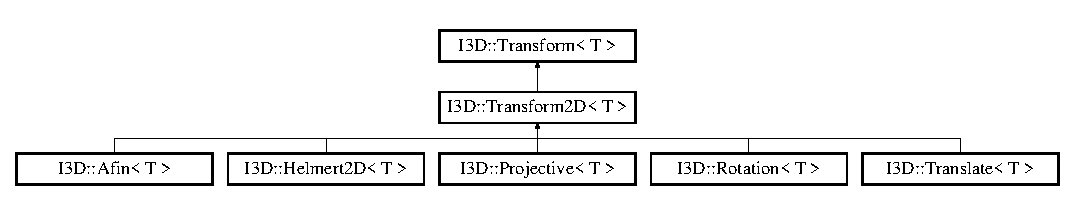
\includegraphics[height=2.255033cm]{class_i3_d_1_1_transform2_d}
\end{center}
\end{figure}
\subsection*{Métodos públicos}
\begin{DoxyCompactItemize}
\item 
\hyperlink{class_i3_d_1_1_transform2_d_a4ff815763fd74155e90ae79564661bb4}{Transform2D} (int n\+\_\+min=0, \hyperlink{group__trf_group_ga175e1580b1ecbc0710ad48060d56c2a3}{transform\+\_\+type} trf\+Type=\hyperlink{group__trf_group_gga175e1580b1ecbc0710ad48060d56c2a3a5b39c8b553c821e7cddc6da64b5bd2ee}{transform\+\_\+type\+::\+D\+E\+F\+A\+U\+LT})
\begin{DoxyCompactList}\small\item\em \hyperlink{class_i3_d_1_1_transform2_d}{Transform2D}. \end{DoxyCompactList}\item 
virtual \hyperlink{class_i3_d_1_1_transform2_d_afe769c95f4b238f62fd9b19ce10e6273}{$\sim$\+Transform2D} ()
\begin{DoxyCompactList}\small\item\em Destructora. \end{DoxyCompactList}\item 
virtual bool \hyperlink{class_i3_d_1_1_transform2_d_a61b1bb9c9a057ceec35c9320447070b9}{compute} (const std\+::vector$<$ T $>$ \&pts1, const std\+::vector$<$ T $>$ \&pts2) override=0
\begin{DoxyCompactList}\small\item\em Calcula los parámetros de transformación. \end{DoxyCompactList}\item 
virtual void \hyperlink{class_i3_d_1_1_transform2_d_a636c5afb2a198d46f7d9c3dc8c1800f1}{transform} (const std\+::vector$<$ T $>$ \&in, std\+::vector$<$ T $>$ $\ast$out, bool b\+Direct=true) const  override=0
\begin{DoxyCompactList}\small\item\em Aplica la transformación. \end{DoxyCompactList}\end{DoxyCompactItemize}
\subsection*{Otros miembros heredados}


\subsection{Documentación del constructor y destructor}
\index{I3\+D\+::\+Transform2D@{I3\+D\+::\+Transform2D}!Transform2D@{Transform2D}}
\index{Transform2D@{Transform2D}!I3\+D\+::\+Transform2D@{I3\+D\+::\+Transform2D}}
\subsubsection[{\texorpdfstring{Transform2\+D(int n\+\_\+min=0, transform\+\_\+type trf\+Type=transform\+\_\+type\+::\+D\+E\+F\+A\+U\+L\+T)}{Transform2D(int n_min=0, transform_type trfType=transform_type::DEFAULT)}}]{\setlength{\rightskip}{0pt plus 5cm}template$<$typename T $>$ {\bf I3\+D\+::\+Transform2D}$<$ T $>$\+::{\bf Transform2D} (
\begin{DoxyParamCaption}
\item[{int}]{n\+\_\+min = {\ttfamily 0}, }
\item[{{\bf transform\+\_\+type}}]{trf\+Type = {\ttfamily {\bf transform\+\_\+type\+::\+D\+E\+F\+A\+U\+LT}}}
\end{DoxyParamCaption}
)\hspace{0.3cm}{\ttfamily [inline]}}\hypertarget{class_i3_d_1_1_transform2_d_a4ff815763fd74155e90ae79564661bb4}{}\label{class_i3_d_1_1_transform2_d_a4ff815763fd74155e90ae79564661bb4}


\hyperlink{class_i3_d_1_1_transform2_d}{Transform2D}. 


\begin{DoxyParams}{Parámetros}
{\em n\+\_\+min} & Número mínimo de puntos necesario para la transformación \\
\hline
\end{DoxyParams}
\index{I3\+D\+::\+Transform2D@{I3\+D\+::\+Transform2D}!````~Transform2D@{$\sim$\+Transform2D}}
\index{````~Transform2D@{$\sim$\+Transform2D}!I3\+D\+::\+Transform2D@{I3\+D\+::\+Transform2D}}
\subsubsection[{\texorpdfstring{$\sim$\+Transform2\+D()}{~Transform2D()}}]{\setlength{\rightskip}{0pt plus 5cm}template$<$typename T $>$ virtual {\bf I3\+D\+::\+Transform2D}$<$ T $>$\+::$\sim${\bf Transform2D} (
\begin{DoxyParamCaption}
{}
\end{DoxyParamCaption}
)\hspace{0.3cm}{\ttfamily [inline]}, {\ttfamily [virtual]}}\hypertarget{class_i3_d_1_1_transform2_d_afe769c95f4b238f62fd9b19ce10e6273}{}\label{class_i3_d_1_1_transform2_d_afe769c95f4b238f62fd9b19ce10e6273}


Destructora. 



\subsection{Documentación de las funciones miembro}
\index{I3\+D\+::\+Transform2D@{I3\+D\+::\+Transform2D}!compute@{compute}}
\index{compute@{compute}!I3\+D\+::\+Transform2D@{I3\+D\+::\+Transform2D}}
\subsubsection[{\texorpdfstring{compute(const std\+::vector$<$ T $>$ \&pts1, const std\+::vector$<$ T $>$ \&pts2) override=0}{compute(const std::vector< T > &pts1, const std::vector< T > &pts2) override=0}}]{\setlength{\rightskip}{0pt plus 5cm}template$<$typename T $>$ virtual bool {\bf I3\+D\+::\+Transform2D}$<$ T $>$\+::compute (
\begin{DoxyParamCaption}
\item[{const std\+::vector$<$ T $>$ \&}]{pts1, }
\item[{const std\+::vector$<$ T $>$ \&}]{pts2}
\end{DoxyParamCaption}
)\hspace{0.3cm}{\ttfamily [override]}, {\ttfamily [pure virtual]}}\hypertarget{class_i3_d_1_1_transform2_d_a61b1bb9c9a057ceec35c9320447070b9}{}\label{class_i3_d_1_1_transform2_d_a61b1bb9c9a057ceec35c9320447070b9}


Calcula los parámetros de transformación. 


\begin{DoxyParams}[1]{Parámetros}
\mbox{\tt in}  & {\em pts1} & Conjunto de puntos en el primero de los sistemas \\
\hline
\mbox{\tt in}  & {\em pts2} & Conjunto de puntos en el segundo de los sistemas \\
\hline
\end{DoxyParams}
\begin{DoxyReturn}{Devuelve}
Verdadero si el calculo se ha efectuado de forma correcta 
\end{DoxyReturn}


Implementa \hyperlink{class_i3_d_1_1_transform_a909a4033f9fab3f091b433b9e2261208}{I3\+D\+::\+Transform$<$ T $>$}.



Implementado en \hyperlink{group__trf2_d_group_gaae888e9e90db1050898b63386252fc88}{I3\+D\+::\+Projective$<$ T $>$}, \hyperlink{group__trf2_d_group_gabe12d714c522dd1bf40f05f28c5aafe0}{I3\+D\+::\+Afin$<$ T $>$}, \hyperlink{group__trf2_d_group_ga300279dee0a002835c25322bd2ea9398}{I3\+D\+::\+Helmert2\+D$<$ T $>$}, \hyperlink{group__trf2_d_group_gae7637f88523deb1879cf8a712820d12e}{I3\+D\+::\+Rotation$<$ T $>$} y \hyperlink{group__trf2_d_group_ga8cab577e50c525caed001caec42a70a6}{I3\+D\+::\+Translate$<$ T $>$}.

\index{I3\+D\+::\+Transform2D@{I3\+D\+::\+Transform2D}!transform@{transform}}
\index{transform@{transform}!I3\+D\+::\+Transform2D@{I3\+D\+::\+Transform2D}}
\subsubsection[{\texorpdfstring{transform(const std\+::vector$<$ T $>$ \&in, std\+::vector$<$ T $>$ $\ast$out, bool b\+Direct=true) const  override=0}{transform(const std::vector< T > &in, std::vector< T > *out, bool bDirect=true) const  override=0}}]{\setlength{\rightskip}{0pt plus 5cm}template$<$typename T $>$ virtual void {\bf I3\+D\+::\+Transform2D}$<$ T $>$\+::transform (
\begin{DoxyParamCaption}
\item[{const std\+::vector$<$ T $>$ \&}]{in, }
\item[{std\+::vector$<$ T $>$ $\ast$}]{out, }
\item[{bool}]{b\+Direct = {\ttfamily true}}
\end{DoxyParamCaption}
) const\hspace{0.3cm}{\ttfamily [override]}, {\ttfamily [pure virtual]}}\hypertarget{class_i3_d_1_1_transform2_d_a636c5afb2a198d46f7d9c3dc8c1800f1}{}\label{class_i3_d_1_1_transform2_d_a636c5afb2a198d46f7d9c3dc8c1800f1}


Aplica la transformación. 


\begin{DoxyParams}[1]{Parámetros}
\mbox{\tt in}  & {\em in} & Puntos de entrada \\
\hline
\mbox{\tt out}  & {\em out} & Puntos de salida \\
\hline
\mbox{\tt in}  & {\em b\+Direct} & Transformación directa (por defecto) \\
\hline
\end{DoxyParams}


Implementa \hyperlink{class_i3_d_1_1_transform_adbec7381bfc66b4a766a00fdf16de0fe}{I3\+D\+::\+Transform$<$ T $>$}.



Implementado en \hyperlink{group__trf2_d_group_ga9339dfc7f978fa6bbb9e2233930e8a3c}{I3\+D\+::\+Projective$<$ T $>$}, \hyperlink{group__trf2_d_group_gae1b65d232072a70d58ec72492a430521}{I3\+D\+::\+Afin$<$ T $>$}, \hyperlink{group__trf2_d_group_gab7354b67b291bf01b3fd045578598fb1}{I3\+D\+::\+Helmert2\+D$<$ T $>$}, \hyperlink{group__trf2_d_group_ga0032788395928aa7419d506981ef03d3}{I3\+D\+::\+Rotation$<$ T $>$} y \hyperlink{group__trf2_d_group_ga1e3ba2120da67c8c4606681c4b82f709}{I3\+D\+::\+Translate$<$ T $>$}.



La documentación para esta clase fue generada a partir del siguiente fichero\+:\begin{DoxyCompactItemize}
\item 
D\+:/\+Desarrollo/tidop/src/\hyperlink{transform_8h}{transform.\+h}\end{DoxyCompactItemize}

\hypertarget{class_i3_d_1_1_transform3_d}{}\section{Referencia de la plantilla de la Clase I3D\+:\+:Transform3D$<$ T $>$}
\label{class_i3_d_1_1_transform3_d}\index{I3\+D\+::\+Transform3\+D$<$ T $>$@{I3\+D\+::\+Transform3\+D$<$ T $>$}}


{\ttfamily \#include $<$transform.\+h$>$}

Diagrama de herencias de I3D\+:\+:Transform3D$<$ T $>$\begin{figure}[H]
\begin{center}
\leavevmode
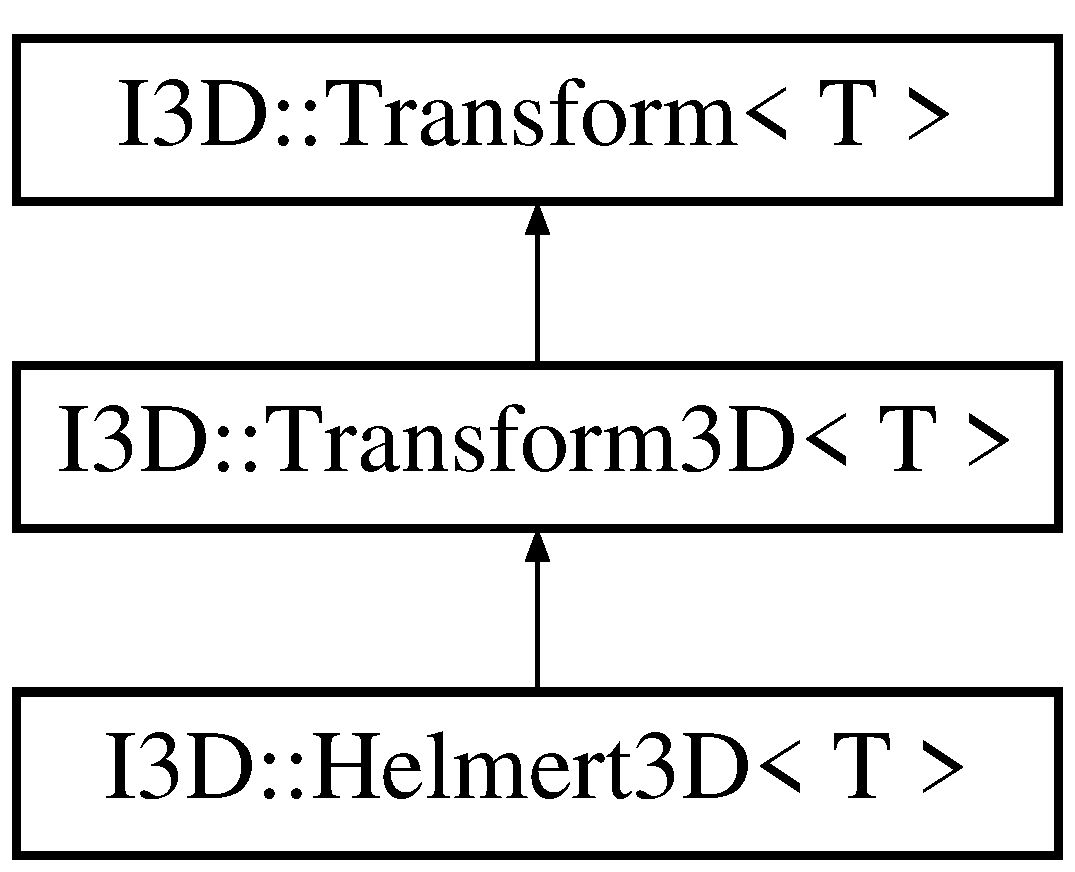
\includegraphics[height=3.000000cm]{class_i3_d_1_1_transform3_d}
\end{center}
\end{figure}
\subsection*{Métodos públicos}
\begin{DoxyCompactItemize}
\item 
\hyperlink{class_i3_d_1_1_transform3_d_a12d7d96b5fe1aa5d151ac1750d2a382d}{Transform3D} (int n\+\_\+min=0, \hyperlink{group__trf_group_ga175e1580b1ecbc0710ad48060d56c2a3}{transform\+\_\+type} trf\+Type=\hyperlink{group__trf_group_gga175e1580b1ecbc0710ad48060d56c2a3a5b39c8b553c821e7cddc6da64b5bd2ee}{transform\+\_\+type\+::\+D\+E\+F\+A\+U\+LT})
\begin{DoxyCompactList}\small\item\em \hyperlink{class_i3_d_1_1_transform}{Transform}. \end{DoxyCompactList}\item 
virtual \hyperlink{class_i3_d_1_1_transform3_d_abc254b877a5a6c382a9571b14ffffa86}{$\sim$\+Transform3D} ()
\begin{DoxyCompactList}\small\item\em Destructora. \end{DoxyCompactList}\item 
virtual bool \hyperlink{class_i3_d_1_1_transform3_d_a3caf93312fc1b3b2ce9f6e88edd9316b}{compute} (const std\+::vector$<$ T $>$ \&pts1, const std\+::vector$<$ T $>$ \&pts2) override=0
\begin{DoxyCompactList}\small\item\em Calcula los parámetros de transformación. \end{DoxyCompactList}\item 
virtual void \hyperlink{class_i3_d_1_1_transform3_d_a229db14f7cd732f5d9ecf01be5ea8bf5}{transform} (const std\+::vector$<$ T $>$ \&in, std\+::vector$<$ T $>$ $\ast$out, bool b\+Direct=true) const  override=0
\begin{DoxyCompactList}\small\item\em Aplica la transformación. \end{DoxyCompactList}\end{DoxyCompactItemize}
\subsection*{Otros miembros heredados}


\subsection{Documentación del constructor y destructor}
\index{I3\+D\+::\+Transform3D@{I3\+D\+::\+Transform3D}!Transform3D@{Transform3D}}
\index{Transform3D@{Transform3D}!I3\+D\+::\+Transform3D@{I3\+D\+::\+Transform3D}}
\subsubsection[{\texorpdfstring{Transform3\+D(int n\+\_\+min=0, transform\+\_\+type trf\+Type=transform\+\_\+type\+::\+D\+E\+F\+A\+U\+L\+T)}{Transform3D(int n_min=0, transform_type trfType=transform_type::DEFAULT)}}]{\setlength{\rightskip}{0pt plus 5cm}template$<$typename T $>$ {\bf I3\+D\+::\+Transform3D}$<$ T $>$\+::{\bf Transform3D} (
\begin{DoxyParamCaption}
\item[{int}]{n\+\_\+min = {\ttfamily 0}, }
\item[{{\bf transform\+\_\+type}}]{trf\+Type = {\ttfamily {\bf transform\+\_\+type\+::\+D\+E\+F\+A\+U\+LT}}}
\end{DoxyParamCaption}
)\hspace{0.3cm}{\ttfamily [inline]}}\hypertarget{class_i3_d_1_1_transform3_d_a12d7d96b5fe1aa5d151ac1750d2a382d}{}\label{class_i3_d_1_1_transform3_d_a12d7d96b5fe1aa5d151ac1750d2a382d}


\hyperlink{class_i3_d_1_1_transform}{Transform}. 

\index{I3\+D\+::\+Transform3D@{I3\+D\+::\+Transform3D}!````~Transform3D@{$\sim$\+Transform3D}}
\index{````~Transform3D@{$\sim$\+Transform3D}!I3\+D\+::\+Transform3D@{I3\+D\+::\+Transform3D}}
\subsubsection[{\texorpdfstring{$\sim$\+Transform3\+D()}{~Transform3D()}}]{\setlength{\rightskip}{0pt plus 5cm}template$<$typename T $>$ virtual {\bf I3\+D\+::\+Transform3D}$<$ T $>$\+::$\sim${\bf Transform3D} (
\begin{DoxyParamCaption}
{}
\end{DoxyParamCaption}
)\hspace{0.3cm}{\ttfamily [inline]}, {\ttfamily [virtual]}}\hypertarget{class_i3_d_1_1_transform3_d_abc254b877a5a6c382a9571b14ffffa86}{}\label{class_i3_d_1_1_transform3_d_abc254b877a5a6c382a9571b14ffffa86}


Destructora. 



\subsection{Documentación de las funciones miembro}
\index{I3\+D\+::\+Transform3D@{I3\+D\+::\+Transform3D}!compute@{compute}}
\index{compute@{compute}!I3\+D\+::\+Transform3D@{I3\+D\+::\+Transform3D}}
\subsubsection[{\texorpdfstring{compute(const std\+::vector$<$ T $>$ \&pts1, const std\+::vector$<$ T $>$ \&pts2) override=0}{compute(const std::vector< T > &pts1, const std::vector< T > &pts2) override=0}}]{\setlength{\rightskip}{0pt plus 5cm}template$<$typename T $>$ virtual bool {\bf I3\+D\+::\+Transform3D}$<$ T $>$\+::compute (
\begin{DoxyParamCaption}
\item[{const std\+::vector$<$ T $>$ \&}]{pts1, }
\item[{const std\+::vector$<$ T $>$ \&}]{pts2}
\end{DoxyParamCaption}
)\hspace{0.3cm}{\ttfamily [override]}, {\ttfamily [pure virtual]}}\hypertarget{class_i3_d_1_1_transform3_d_a3caf93312fc1b3b2ce9f6e88edd9316b}{}\label{class_i3_d_1_1_transform3_d_a3caf93312fc1b3b2ce9f6e88edd9316b}


Calcula los parámetros de transformación. 


\begin{DoxyParams}[1]{Parámetros}
\mbox{\tt in}  & {\em pts1} & Conjunto de puntos en el primero de los sistemas \\
\hline
\mbox{\tt in}  & {\em pts2} & Conjunto de puntos en el segundo de los sistemas \\
\hline
\end{DoxyParams}
\begin{DoxyReturn}{Devuelve}
Verdadero si el calculo se ha efectuado de forma correcta 
\end{DoxyReturn}


Implementa \hyperlink{class_i3_d_1_1_transform_a909a4033f9fab3f091b433b9e2261208}{I3\+D\+::\+Transform$<$ T $>$}.



Implementado en \hyperlink{group__trf3_d_group_gaf6c9d07daaca435365b84688326885e3}{I3\+D\+::\+Helmert3\+D$<$ T $>$}.

\index{I3\+D\+::\+Transform3D@{I3\+D\+::\+Transform3D}!transform@{transform}}
\index{transform@{transform}!I3\+D\+::\+Transform3D@{I3\+D\+::\+Transform3D}}
\subsubsection[{\texorpdfstring{transform(const std\+::vector$<$ T $>$ \&in, std\+::vector$<$ T $>$ $\ast$out, bool b\+Direct=true) const  override=0}{transform(const std::vector< T > &in, std::vector< T > *out, bool bDirect=true) const  override=0}}]{\setlength{\rightskip}{0pt plus 5cm}template$<$typename T $>$ virtual void {\bf I3\+D\+::\+Transform3D}$<$ T $>$\+::transform (
\begin{DoxyParamCaption}
\item[{const std\+::vector$<$ T $>$ \&}]{in, }
\item[{std\+::vector$<$ T $>$ $\ast$}]{out, }
\item[{bool}]{b\+Direct = {\ttfamily true}}
\end{DoxyParamCaption}
) const\hspace{0.3cm}{\ttfamily [override]}, {\ttfamily [pure virtual]}}\hypertarget{class_i3_d_1_1_transform3_d_a229db14f7cd732f5d9ecf01be5ea8bf5}{}\label{class_i3_d_1_1_transform3_d_a229db14f7cd732f5d9ecf01be5ea8bf5}


Aplica la transformación. 


\begin{DoxyParams}[1]{Parámetros}
\mbox{\tt in}  & {\em in} & Puntos de entrada \\
\hline
\mbox{\tt out}  & {\em out} & Puntos de salida \\
\hline
\mbox{\tt in}  & {\em b\+Direct} & Transformación directa (por defecto) \\
\hline
\end{DoxyParams}


Implementa \hyperlink{class_i3_d_1_1_transform_adbec7381bfc66b4a766a00fdf16de0fe}{I3\+D\+::\+Transform$<$ T $>$}.



Implementado en \hyperlink{group__trf3_d_group_ga986e7df721d9a5bb12a0eed3ab10f419}{I3\+D\+::\+Helmert3\+D$<$ T $>$}.



La documentación para esta clase fue generada a partir del siguiente fichero\+:\begin{DoxyCompactItemize}
\item 
C\+:/\+Desarrollo/tidop/src/\hyperlink{transform_8h}{transform.\+h}\end{DoxyCompactItemize}

\hypertarget{class_i3_d_1_1_translate}{}\section{Referencia de la plantilla de la Clase I3D\+:\+:Translate$<$ T $>$}
\label{class_i3_d_1_1_translate}\index{I3\+D\+::\+Translate$<$ T $>$@{I3\+D\+::\+Translate$<$ T $>$}}


Traslación.  




{\ttfamily \#include $<$transform.\+h$>$}

Diagrama de herencias de I3D\+:\+:Translate$<$ T $>$\begin{figure}[H]
\begin{center}
\leavevmode
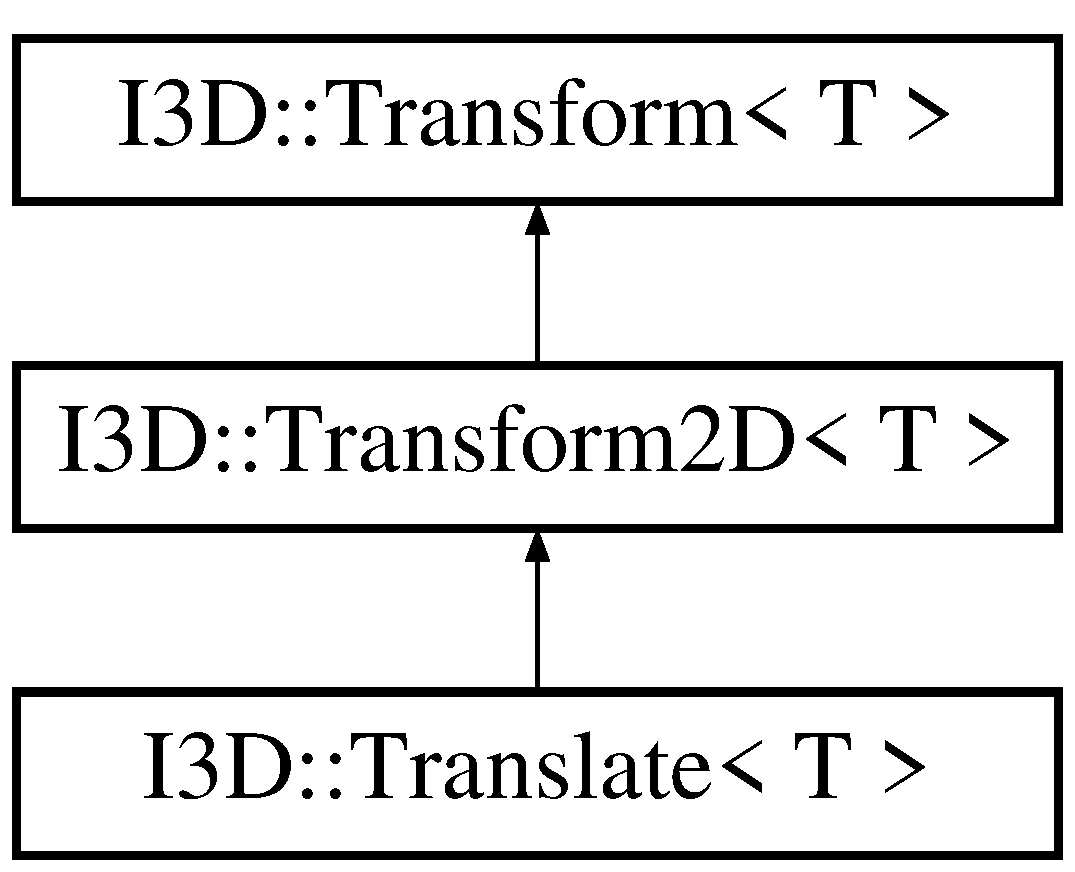
\includegraphics[height=3.000000cm]{class_i3_d_1_1_translate}
\end{center}
\end{figure}
\subsection*{Métodos públicos}
\begin{DoxyCompactItemize}
\item 
\hyperlink{class_i3_d_1_1_translate_aa65ece5d3be0809aedb1dd05073aa51c}{Translate} ()
\begin{DoxyCompactList}\small\item\em Constructora por defecto. \end{DoxyCompactList}\item 
\hyperlink{class_i3_d_1_1_translate_af75eefcf1cc5dfae68bf6a59dc712884}{Translate} (\hyperlink{class_i3_d_1_1_transform_ac087b4b8b9acb1b11a6caa2231d598c7}{sub\+\_\+type} x0, \hyperlink{class_i3_d_1_1_transform_ac087b4b8b9acb1b11a6caa2231d598c7}{sub\+\_\+type} y0)
\begin{DoxyCompactList}\small\item\em Constructora. \end{DoxyCompactList}\item 
bool \hyperlink{group__trf2_d_group_ga8cab577e50c525caed001caec42a70a6}{compute} (const std\+::vector$<$ T $>$ \&pts1, const std\+::vector$<$ T $>$ \&pts2) override
\begin{DoxyCompactList}\small\item\em Calculo de la traslación. \end{DoxyCompactList}\item 
\hyperlink{class_i3_d_1_1_transform_ac087b4b8b9acb1b11a6caa2231d598c7}{sub\+\_\+type} \hyperlink{class_i3_d_1_1_translate_ae18184337b23daeaf131ce945153b2ef}{get\+TranslationX} ()
\begin{DoxyCompactList}\small\item\em Devuelve el desplazamiento en x de la transformación. \end{DoxyCompactList}\item 
\hyperlink{class_i3_d_1_1_transform_ac087b4b8b9acb1b11a6caa2231d598c7}{sub\+\_\+type} \hyperlink{class_i3_d_1_1_translate_a29f7cc2a3a2060c78c8070175e648b11}{get\+TranslationY} ()
\begin{DoxyCompactList}\small\item\em Devuelve el desplazamiento en y de la transformación. \end{DoxyCompactList}\item 
void \hyperlink{group__trf2_d_group_ga93831181f6cf779c0a7097b348c9c879}{set\+Translation} (\hyperlink{class_i3_d_1_1_transform_ac087b4b8b9acb1b11a6caa2231d598c7}{sub\+\_\+type} x0, \hyperlink{class_i3_d_1_1_transform_ac087b4b8b9acb1b11a6caa2231d598c7}{sub\+\_\+type} y0)
\begin{DoxyCompactList}\small\item\em Establece los valores de desplazamiento. \end{DoxyCompactList}\item 
void \hyperlink{group__trf2_d_group_gaa4a82205fd57f86aed9338054104a22f}{set\+TranslationX} (\hyperlink{class_i3_d_1_1_transform_ac087b4b8b9acb1b11a6caa2231d598c7}{sub\+\_\+type} x0)
\begin{DoxyCompactList}\small\item\em Establece el desplazamiento en el eje x. \end{DoxyCompactList}\item 
void \hyperlink{group__trf2_d_group_gaed6d19903cf0da2cd1ced22381ec223b}{set\+TranslationY} (\hyperlink{class_i3_d_1_1_transform_ac087b4b8b9acb1b11a6caa2231d598c7}{sub\+\_\+type} y0)
\begin{DoxyCompactList}\small\item\em Establece el desplazamiento en el eje y. \end{DoxyCompactList}\item 
void \hyperlink{group__trf2_d_group_ga1e3ba2120da67c8c4606681c4b82f709}{transform} (const std\+::vector$<$ T $>$ \&in, std\+::vector$<$ T $>$ $\ast$out, bool b\+Direct=true) const  override
\begin{DoxyCompactList}\small\item\em Transforma un conjunto de puntos en otro aplicando una traslación. \end{DoxyCompactList}\item 
void \hyperlink{group__trf2_d_group_ga8be3570501a8efb7a67210bb24d5218c}{transform} (const std\+::vector$<$ \hyperlink{class_i3_d_1_1_segment}{Segment}$<$ \hyperlink{class_i3_d_1_1_transform_ac087b4b8b9acb1b11a6caa2231d598c7}{sub\+\_\+type} $>$$>$ \&in, std\+::vector$<$ \hyperlink{class_i3_d_1_1_segment}{Segment}$<$ \hyperlink{class_i3_d_1_1_transform_ac087b4b8b9acb1b11a6caa2231d598c7}{sub\+\_\+type} $>$$>$ $\ast$out, bool b\+Direct=true) const 
\begin{DoxyCompactList}\small\item\em Transforma un conjunto de segmentos en otro aplicando una traslación. \end{DoxyCompactList}\item 
void \hyperlink{group__trf2_d_group_ga2f30e8ab65a36498c27994e2887deb80}{transform} (const T \&in, T $\ast$out, bool b\+Direct=true) const 
\begin{DoxyCompactList}\small\item\em Aplica una traslación a un punto. \end{DoxyCompactList}\item 
T \hyperlink{group__trf2_d_group_gafdec629c6bb3f71d71934c43d4a54b74}{transform} (const T \&pt, bool b\+Direct=true) const 
\begin{DoxyCompactList}\small\item\em Aplica una traslación a un punto. \end{DoxyCompactList}\end{DoxyCompactItemize}
\subsection*{Otros miembros heredados}


\subsection{Descripción detallada}
\subsubsection*{template$<$typename T$>$\\*
class I3\+D\+::\+Translate$<$ T $>$}

Traslación. 

Transformación que aplica una traslación en el plano a un conjunto de puntos 

\subsection{Documentación del constructor y destructor}
\index{I3\+D\+::\+Translate@{I3\+D\+::\+Translate}!Translate@{Translate}}
\index{Translate@{Translate}!I3\+D\+::\+Translate@{I3\+D\+::\+Translate}}
\subsubsection[{\texorpdfstring{Translate()}{Translate()}}]{\setlength{\rightskip}{0pt plus 5cm}template$<$typename T $>$ {\bf I3\+D\+::\+Translate}$<$ T $>$\+::{\bf Translate} (
\begin{DoxyParamCaption}
{}
\end{DoxyParamCaption}
)\hspace{0.3cm}{\ttfamily [inline]}}\hypertarget{class_i3_d_1_1_translate_aa65ece5d3be0809aedb1dd05073aa51c}{}\label{class_i3_d_1_1_translate_aa65ece5d3be0809aedb1dd05073aa51c}


Constructora por defecto. 

\index{I3\+D\+::\+Translate@{I3\+D\+::\+Translate}!Translate@{Translate}}
\index{Translate@{Translate}!I3\+D\+::\+Translate@{I3\+D\+::\+Translate}}
\subsubsection[{\texorpdfstring{Translate(sub\+\_\+type x0, sub\+\_\+type y0)}{Translate(sub_type x0, sub_type y0)}}]{\setlength{\rightskip}{0pt plus 5cm}template$<$typename T $>$ {\bf I3\+D\+::\+Translate}$<$ T $>$\+::{\bf Translate} (
\begin{DoxyParamCaption}
\item[{{\bf sub\+\_\+type}}]{x0, }
\item[{{\bf sub\+\_\+type}}]{y0}
\end{DoxyParamCaption}
)\hspace{0.3cm}{\ttfamily [inline]}}\hypertarget{class_i3_d_1_1_translate_af75eefcf1cc5dfae68bf6a59dc712884}{}\label{class_i3_d_1_1_translate_af75eefcf1cc5dfae68bf6a59dc712884}


Constructora. 


\begin{DoxyParams}[1]{Parámetros}
\mbox{\tt in}  & {\em x0} & Traslación en el eje X \\
\hline
\mbox{\tt in}  & {\em y0} & Traslación en el eje Y \\
\hline
\end{DoxyParams}


\subsection{Documentación de las funciones miembro}
\index{I3\+D\+::\+Translate@{I3\+D\+::\+Translate}!get\+TranslationX@{get\+TranslationX}}
\index{get\+TranslationX@{get\+TranslationX}!I3\+D\+::\+Translate@{I3\+D\+::\+Translate}}
\subsubsection[{\texorpdfstring{get\+Translation\+X()}{getTranslationX()}}]{\setlength{\rightskip}{0pt plus 5cm}template$<$typename T $>$ {\bf sub\+\_\+type} {\bf I3\+D\+::\+Translate}$<$ T $>$\+::get\+TranslationX (
\begin{DoxyParamCaption}
{}
\end{DoxyParamCaption}
)\hspace{0.3cm}{\ttfamily [inline]}}\hypertarget{class_i3_d_1_1_translate_ae18184337b23daeaf131ce945153b2ef}{}\label{class_i3_d_1_1_translate_ae18184337b23daeaf131ce945153b2ef}


Devuelve el desplazamiento en x de la transformación. 

\begin{DoxyReturn}{Devuelve}
Desplazamiento en el eje x 
\end{DoxyReturn}
\index{I3\+D\+::\+Translate@{I3\+D\+::\+Translate}!get\+TranslationY@{get\+TranslationY}}
\index{get\+TranslationY@{get\+TranslationY}!I3\+D\+::\+Translate@{I3\+D\+::\+Translate}}
\subsubsection[{\texorpdfstring{get\+Translation\+Y()}{getTranslationY()}}]{\setlength{\rightskip}{0pt plus 5cm}template$<$typename T $>$ {\bf sub\+\_\+type} {\bf I3\+D\+::\+Translate}$<$ T $>$\+::get\+TranslationY (
\begin{DoxyParamCaption}
{}
\end{DoxyParamCaption}
)\hspace{0.3cm}{\ttfamily [inline]}}\hypertarget{class_i3_d_1_1_translate_a29f7cc2a3a2060c78c8070175e648b11}{}\label{class_i3_d_1_1_translate_a29f7cc2a3a2060c78c8070175e648b11}


Devuelve el desplazamiento en y de la transformación. 

\begin{DoxyReturn}{Devuelve}
Desplazamiento en el eje y 
\end{DoxyReturn}


La documentación para esta clase fue generada a partir del siguiente fichero\+:\begin{DoxyCompactItemize}
\item 
D\+:/\+Desarrollo/tidop/src/\hyperlink{transform_8h}{transform.\+h}\end{DoxyCompactItemize}

\hypertarget{class_i3_d_1_1_trf_multiple}{}\section{Referencia de la plantilla de la Clase I3D\+:\+:Trf\+Multiple$<$ T $>$}
\label{class_i3_d_1_1_trf_multiple}\index{I3\+D\+::\+Trf\+Multiple$<$ T $>$@{I3\+D\+::\+Trf\+Multiple$<$ T $>$}}


Transformación multiple.  




{\ttfamily \#include $<$transform.\+h$>$}

Diagrama de herencias de I3D\+:\+:Trf\+Multiple$<$ T $>$\begin{figure}[H]
\begin{center}
\leavevmode
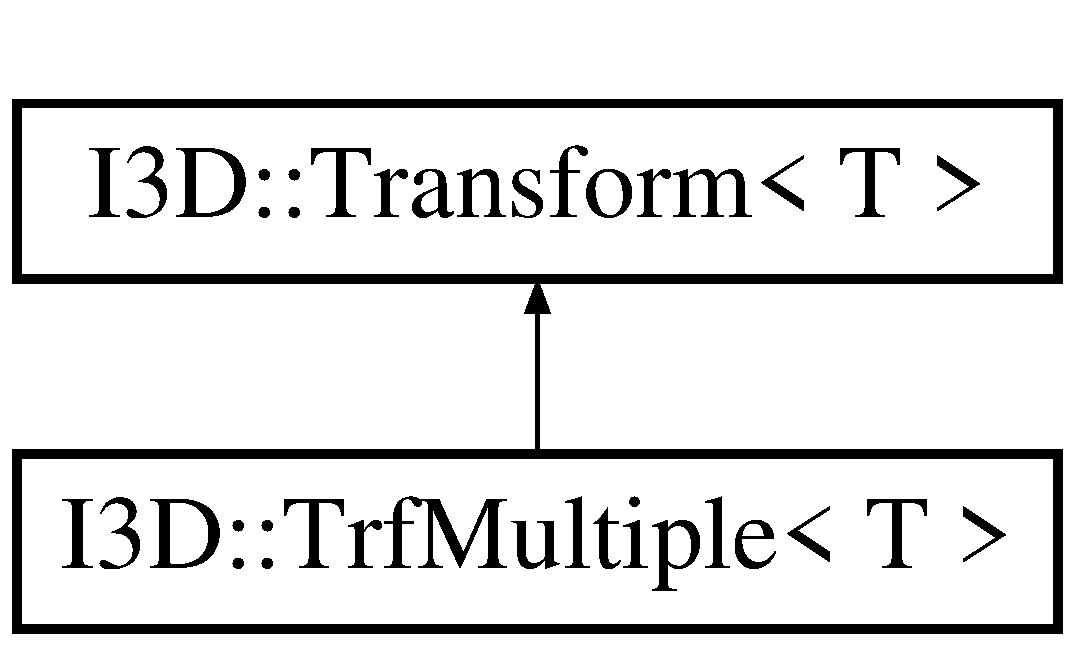
\includegraphics[height=2.000000cm]{class_i3_d_1_1_trf_multiple}
\end{center}
\end{figure}
\subsection*{Métodos públicos}
\begin{DoxyCompactItemize}
\item 
\hyperlink{class_i3_d_1_1_trf_multiple_a30d9f42f909ca7cf936845acef6d6fdf}{Trf\+Multiple} ()
\begin{DoxyCompactList}\small\item\em Constructora. \end{DoxyCompactList}\item 
\hyperlink{class_i3_d_1_1_trf_multiple_a587edd2f69bff8f145c79c8934dc2895}{Trf\+Multiple} (std\+::initializer\+\_\+list$<$ std\+::shared\+\_\+ptr$<$ \hyperlink{class_i3_d_1_1_transform}{Transform}$<$ T $>$$>$$>$ transf\+List)
\begin{DoxyCompactList}\small\item\em Constructor de lista. \end{DoxyCompactList}\item 
\hyperlink{class_i3_d_1_1_trf_multiple_a474109b2a2b9040288139f28b3a0af6b}{$\sim$\+Trf\+Multiple} ()
\begin{DoxyCompactList}\small\item\em Destructora. \end{DoxyCompactList}\item 
void \hyperlink{class_i3_d_1_1_trf_multiple_a214c54fe571166735d0fda5f2a827642}{add} (std\+::shared\+\_\+ptr$<$ \hyperlink{class_i3_d_1_1_transform}{Transform}$<$ T $>$$>$ trf)
\begin{DoxyCompactList}\small\item\em Añade una nueva transformación a la lista. \end{DoxyCompactList}\item 
void \hyperlink{class_i3_d_1_1_trf_multiple_ab7cd324176621b83076f1a3db881c6ca}{clear} ()
\begin{DoxyCompactList}\small\item\em Borra las transformaciones. \end{DoxyCompactList}\item 
bool \hyperlink{group__trf_group_ga30e6b58e89d4ad3657e1b6a74edc22cc}{compute} (const std\+::vector$<$ T $>$ \&pts1, const std\+::vector$<$ T $>$ \&pts2) override
\begin{DoxyCompactList}\small\item\em Calcula los parámetros de transformación. \end{DoxyCompactList}\item 
void \hyperlink{group__trf_group_gad8eb1ca9e9b9c6e6d30f1f1b15dee818}{transform} (const std\+::vector$<$ T $>$ \&in, std\+::vector$<$ T $>$ $\ast$out, bool b\+Direct=true) const  override
\begin{DoxyCompactList}\small\item\em Aplica la transformación. \end{DoxyCompactList}\end{DoxyCompactItemize}
\subsection*{Otros miembros heredados}


\subsection{Descripción detallada}
\subsubsection*{template$<$typename T$>$\\*
class I3\+D\+::\+Trf\+Multiple$<$ T $>$}

Transformación multiple. 

Una transformación multiple permite agrupar varias transformaciones de forma que se ejecutan a la vez (consecutivamente). 

\subsection{Documentación del constructor y destructor}
\index{I3\+D\+::\+Trf\+Multiple@{I3\+D\+::\+Trf\+Multiple}!Trf\+Multiple@{Trf\+Multiple}}
\index{Trf\+Multiple@{Trf\+Multiple}!I3\+D\+::\+Trf\+Multiple@{I3\+D\+::\+Trf\+Multiple}}
\subsubsection[{\texorpdfstring{Trf\+Multiple()}{TrfMultiple()}}]{\setlength{\rightskip}{0pt plus 5cm}template$<$typename T $>$ {\bf I3\+D\+::\+Trf\+Multiple}$<$ T $>$\+::{\bf Trf\+Multiple} (
\begin{DoxyParamCaption}
{}
\end{DoxyParamCaption}
)\hspace{0.3cm}{\ttfamily [inline]}}\hypertarget{class_i3_d_1_1_trf_multiple_a30d9f42f909ca7cf936845acef6d6fdf}{}\label{class_i3_d_1_1_trf_multiple_a30d9f42f909ca7cf936845acef6d6fdf}


Constructora. 

\index{I3\+D\+::\+Trf\+Multiple@{I3\+D\+::\+Trf\+Multiple}!Trf\+Multiple@{Trf\+Multiple}}
\index{Trf\+Multiple@{Trf\+Multiple}!I3\+D\+::\+Trf\+Multiple@{I3\+D\+::\+Trf\+Multiple}}
\subsubsection[{\texorpdfstring{Trf\+Multiple(std\+::initializer\+\_\+list$<$ std\+::shared\+\_\+ptr$<$ Transform$<$ T $>$$>$$>$ transf\+List)}{TrfMultiple(std::initializer_list< std::shared_ptr< Transform< T >>> transfList)}}]{\setlength{\rightskip}{0pt plus 5cm}template$<$typename T $>$ {\bf I3\+D\+::\+Trf\+Multiple}$<$ T $>$\+::{\bf Trf\+Multiple} (
\begin{DoxyParamCaption}
\item[{std\+::initializer\+\_\+list$<$ std\+::shared\+\_\+ptr$<$ {\bf Transform}$<$ T $>$$>$$>$}]{transf\+List}
\end{DoxyParamCaption}
)\hspace{0.3cm}{\ttfamily [inline]}}\hypertarget{class_i3_d_1_1_trf_multiple_a587edd2f69bff8f145c79c8934dc2895}{}\label{class_i3_d_1_1_trf_multiple_a587edd2f69bff8f145c79c8934dc2895}


Constructor de lista. 


\begin{DoxyParams}[1]{Parámetros}
\mbox{\tt in}  & {\em transf\+List} & listado de transformaciones \\
\hline
\end{DoxyParams}
\index{I3\+D\+::\+Trf\+Multiple@{I3\+D\+::\+Trf\+Multiple}!````~Trf\+Multiple@{$\sim$\+Trf\+Multiple}}
\index{````~Trf\+Multiple@{$\sim$\+Trf\+Multiple}!I3\+D\+::\+Trf\+Multiple@{I3\+D\+::\+Trf\+Multiple}}
\subsubsection[{\texorpdfstring{$\sim$\+Trf\+Multiple()}{~TrfMultiple()}}]{\setlength{\rightskip}{0pt plus 5cm}template$<$typename T $>$ {\bf I3\+D\+::\+Trf\+Multiple}$<$ T $>$\+::$\sim${\bf Trf\+Multiple} (
\begin{DoxyParamCaption}
{}
\end{DoxyParamCaption}
)\hspace{0.3cm}{\ttfamily [inline]}}\hypertarget{class_i3_d_1_1_trf_multiple_a474109b2a2b9040288139f28b3a0af6b}{}\label{class_i3_d_1_1_trf_multiple_a474109b2a2b9040288139f28b3a0af6b}


Destructora. 



\subsection{Documentación de las funciones miembro}
\index{I3\+D\+::\+Trf\+Multiple@{I3\+D\+::\+Trf\+Multiple}!add@{add}}
\index{add@{add}!I3\+D\+::\+Trf\+Multiple@{I3\+D\+::\+Trf\+Multiple}}
\subsubsection[{\texorpdfstring{add(std\+::shared\+\_\+ptr$<$ Transform$<$ T $>$$>$ trf)}{add(std::shared_ptr< Transform< T >> trf)}}]{\setlength{\rightskip}{0pt plus 5cm}template$<$typename T $>$ void {\bf I3\+D\+::\+Trf\+Multiple}$<$ T $>$\+::add (
\begin{DoxyParamCaption}
\item[{std\+::shared\+\_\+ptr$<$ {\bf Transform}$<$ T $>$$>$}]{trf}
\end{DoxyParamCaption}
)\hspace{0.3cm}{\ttfamily [inline]}}\hypertarget{class_i3_d_1_1_trf_multiple_a214c54fe571166735d0fda5f2a827642}{}\label{class_i3_d_1_1_trf_multiple_a214c54fe571166735d0fda5f2a827642}


Añade una nueva transformación a la lista. 


\begin{DoxyParams}[1]{Parámetros}
\mbox{\tt in}  & {\em trf} & Transformación que se añade \\
\hline
\end{DoxyParams}
\index{I3\+D\+::\+Trf\+Multiple@{I3\+D\+::\+Trf\+Multiple}!clear@{clear}}
\index{clear@{clear}!I3\+D\+::\+Trf\+Multiple@{I3\+D\+::\+Trf\+Multiple}}
\subsubsection[{\texorpdfstring{clear()}{clear()}}]{\setlength{\rightskip}{0pt plus 5cm}template$<$typename T $>$ void {\bf I3\+D\+::\+Trf\+Multiple}$<$ T $>$\+::clear (
\begin{DoxyParamCaption}
{}
\end{DoxyParamCaption}
)\hspace{0.3cm}{\ttfamily [inline]}}\hypertarget{class_i3_d_1_1_trf_multiple_ab7cd324176621b83076f1a3db881c6ca}{}\label{class_i3_d_1_1_trf_multiple_ab7cd324176621b83076f1a3db881c6ca}


Borra las transformaciones. 



La documentación para esta clase fue generada a partir del siguiente fichero\+:\begin{DoxyCompactItemize}
\item 
D\+:/\+Desarrollo/tidop/src/\hyperlink{transform_8h}{transform.\+h}\end{DoxyCompactItemize}

\hypertarget{class_i3_d_1_1_trf_perspective}{}\section{Referencia de la plantilla de la Clase I3D\+:\+:Trf\+Perspective$<$ T $>$}
\label{class_i3_d_1_1_trf_perspective}\index{I3\+D\+::\+Trf\+Perspective$<$ T $>$@{I3\+D\+::\+Trf\+Perspective$<$ T $>$}}


perspective  




{\ttfamily \#include $<$transform.\+h$>$}

Diagrama de herencias de I3D\+:\+:Trf\+Perspective$<$ T $>$\begin{figure}[H]
\begin{center}
\leavevmode
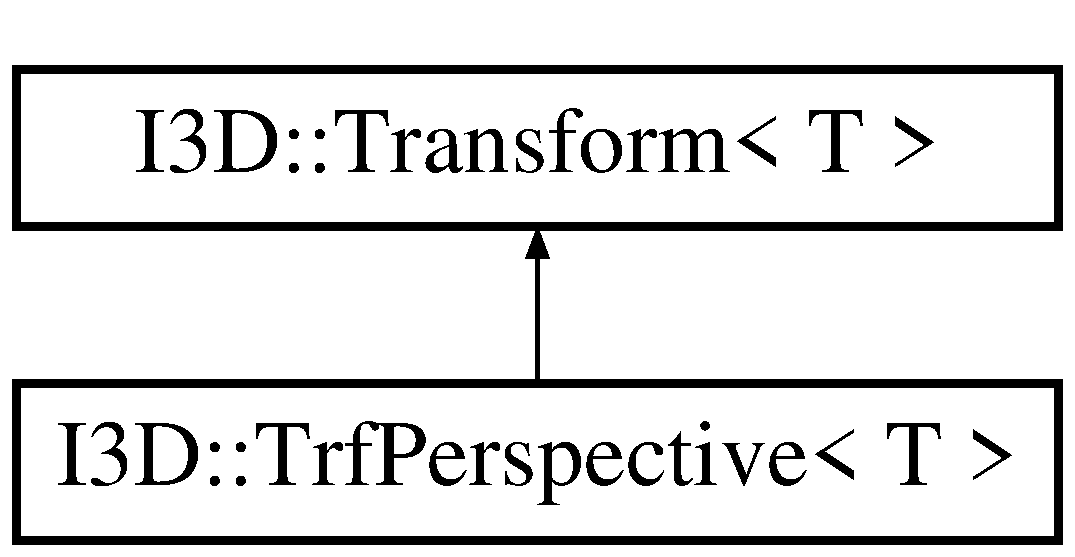
\includegraphics[height=2.000000cm]{class_i3_d_1_1_trf_perspective}
\end{center}
\end{figure}
\subsection*{Métodos públicos}
\begin{DoxyCompactItemize}
\item 
\hyperlink{class_i3_d_1_1_trf_perspective_a6f0b52bf124ae94eb6cab55fbcfb85b7}{Trf\+Perspective} ()
\item 
\hyperlink{class_i3_d_1_1_trf_perspective_a6cab003ac2b49d52ae8b29a2ceea99f1}{$\sim$\+Trf\+Perspective} ()
\item 
bool \hyperlink{group__trf2_d_group_gaf4d7f0809edd08cc847f3df1db43055e}{compute} (const std\+::vector$<$ T $>$ \&pts1, const std\+::vector$<$ T $>$ \&pts2) override
\begin{DoxyCompactList}\small\item\em Calcula los parámetros de transformación. \end{DoxyCompactList}\item 
void \hyperlink{group__trf2_d_group_ga0742db3f66df991a7e4a2d1d91d1a783}{transform} (const std\+::vector$<$ T $>$ \&in, std\+::vector$<$ T $>$ $\ast$out, bool b\+Direct=true) const  override
\begin{DoxyCompactList}\small\item\em Aplica la transformación. \end{DoxyCompactList}\end{DoxyCompactItemize}
\subsection*{Otros miembros heredados}


\subsection{Descripción detallada}
\subsubsection*{template$<$typename T$>$\\*
class I3\+D\+::\+Trf\+Perspective$<$ T $>$}

perspective 

\subsection{Documentación del constructor y destructor}
\index{I3\+D\+::\+Trf\+Perspective@{I3\+D\+::\+Trf\+Perspective}!Trf\+Perspective@{Trf\+Perspective}}
\index{Trf\+Perspective@{Trf\+Perspective}!I3\+D\+::\+Trf\+Perspective@{I3\+D\+::\+Trf\+Perspective}}
\subsubsection[{\texorpdfstring{Trf\+Perspective()}{TrfPerspective()}}]{\setlength{\rightskip}{0pt plus 5cm}template$<$typename T $>$ {\bf I3\+D\+::\+Trf\+Perspective}$<$ T $>$\+::{\bf Trf\+Perspective} (
\begin{DoxyParamCaption}
{}
\end{DoxyParamCaption}
)\hspace{0.3cm}{\ttfamily [inline]}}\hypertarget{class_i3_d_1_1_trf_perspective_a6f0b52bf124ae94eb6cab55fbcfb85b7}{}\label{class_i3_d_1_1_trf_perspective_a6f0b52bf124ae94eb6cab55fbcfb85b7}
\index{I3\+D\+::\+Trf\+Perspective@{I3\+D\+::\+Trf\+Perspective}!````~Trf\+Perspective@{$\sim$\+Trf\+Perspective}}
\index{````~Trf\+Perspective@{$\sim$\+Trf\+Perspective}!I3\+D\+::\+Trf\+Perspective@{I3\+D\+::\+Trf\+Perspective}}
\subsubsection[{\texorpdfstring{$\sim$\+Trf\+Perspective()}{~TrfPerspective()}}]{\setlength{\rightskip}{0pt plus 5cm}template$<$typename T $>$ {\bf I3\+D\+::\+Trf\+Perspective}$<$ T $>$\+::$\sim${\bf Trf\+Perspective} (
\begin{DoxyParamCaption}
{}
\end{DoxyParamCaption}
)\hspace{0.3cm}{\ttfamily [inline]}}\hypertarget{class_i3_d_1_1_trf_perspective_a6cab003ac2b49d52ae8b29a2ceea99f1}{}\label{class_i3_d_1_1_trf_perspective_a6cab003ac2b49d52ae8b29a2ceea99f1}


La documentación para esta clase fue generada a partir del siguiente fichero\+:\begin{DoxyCompactItemize}
\item 
C\+:/\+Desarrollo/tidop/src/\hyperlink{transform_8h}{transform.\+h}\end{DoxyCompactItemize}

\hypertarget{class_i3_d_1_1_video_stream}{}\section{Referencia de la Clase I3D\+:\+:Video\+Stream}
\label{class_i3_d_1_1_video_stream}\index{I3\+D\+::\+Video\+Stream@{I3\+D\+::\+Video\+Stream}}


Clase para el manejo de video.  




{\ttfamily \#include $<$Video\+Stream.\+h$>$}

Diagrama de herencias de I3D\+:\+:Video\+Stream\begin{figure}[H]
\begin{center}
\leavevmode
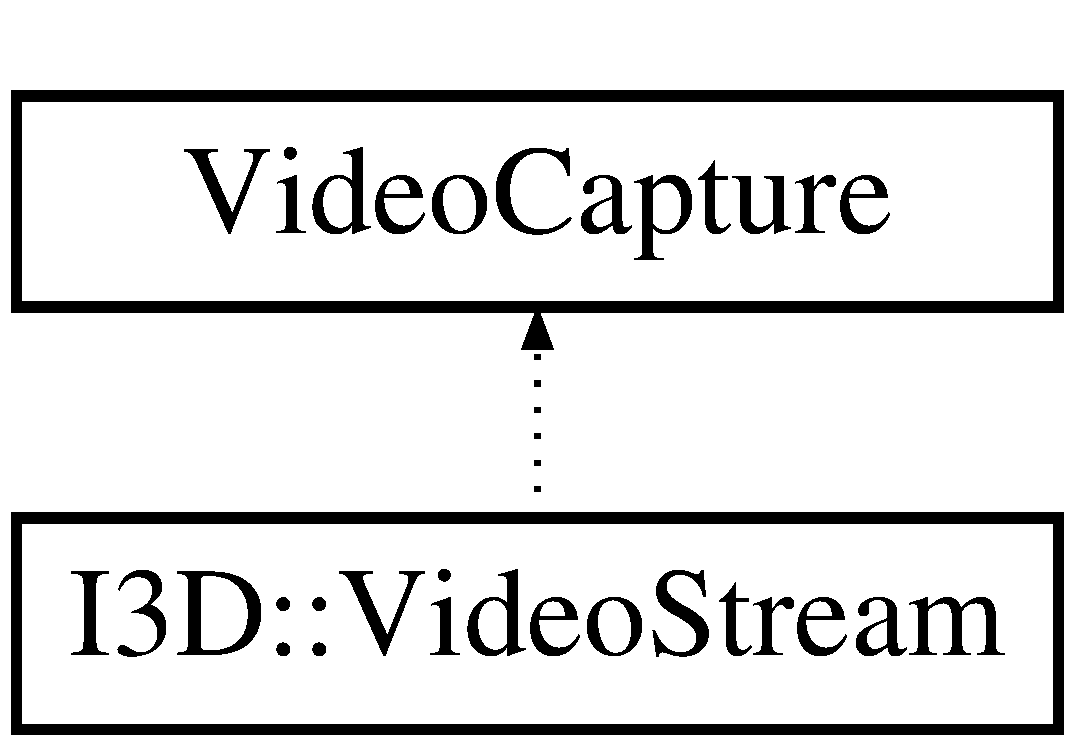
\includegraphics[height=2.000000cm]{class_i3_d_1_1_video_stream}
\end{center}
\end{figure}
\subsection*{Métodos públicos}
\begin{DoxyCompactItemize}
\item 
\hyperlink{class_i3_d_1_1_video_stream_a93cc6df0a8514eefcb1bf85a95168f34}{Video\+Stream} ()
\begin{DoxyCompactList}\small\item\em Constructora I3\+D\+Video\+Stream. \end{DoxyCompactList}\item 
\hyperlink{class_i3_d_1_1_video_stream_aaa046c13d80ba4dae903346ac2f512fe}{Video\+Stream} (const char $\ast$file)
\begin{DoxyCompactList}\small\item\em Constructora I3\+D\+Video\+Stream. \end{DoxyCompactList}\item 
\hyperlink{class_i3_d_1_1_video_stream_a3034afe657b7337a8e697b26727b3edd}{$\sim$\+Video\+Stream} ()
\begin{DoxyCompactList}\small\item\em Destructora I3\+D\+Video\+Stream. \end{DoxyCompactList}\item 
double \hyperlink{class_i3_d_1_1_video_stream_ae9911a61f3c3196ad7efcb49cd3a9595}{fps} ()
\begin{DoxyCompactList}\small\item\em Frames por segundo del video. \end{DoxyCompactList}\item 
double \hyperlink{class_i3_d_1_1_video_stream_a8deb6c7defcf5bbc01be2ae48c68167e}{get\+Current\+Frame} ()
\begin{DoxyCompactList}\small\item\em Frame de video actual. \end{DoxyCompactList}\item 
double \hyperlink{class_i3_d_1_1_video_stream_a2416c9205c1ce815d6692153d162635d}{get\+Frame\+Count} ()
\begin{DoxyCompactList}\small\item\em Número de frames del video. \end{DoxyCompactList}\item 
cv\+::\+Size \hyperlink{class_i3_d_1_1_video_stream_adcd195f78a21b8009b1069643fed5a14}{get\+Frame\+Size} ()
\begin{DoxyCompactList}\small\item\em Devuelve el ancho y alto de los frames de salida. \end{DoxyCompactList}\item 
cv\+::\+Size \hyperlink{class_i3_d_1_1_video_stream_ac17f6f75aec2c161070d794715033023}{get\+Size} ()
\begin{DoxyCompactList}\small\item\em Ancho y alto del video. \end{DoxyCompactList}\item 
bool \hyperlink{class_i3_d_1_1_video_stream_a11947a15a95cf62d68b987d16887bd23}{is\+Opened} ()
\begin{DoxyCompactList}\small\item\em Comprueba si el video está abierto. \end{DoxyCompactList}\item 
bool \hyperlink{class_i3_d_1_1_video_stream_ad19ab11928372741ddb1ab0328d9aa8f}{next\+Frame} (cv\+::\+Mat \&vf)
\begin{DoxyCompactList}\small\item\em Next\+Frame. \end{DoxyCompactList}\item 
bool \hyperlink{class_i3_d_1_1_video_stream_a72e10a1973eecdf0b8b87fbefbb56473}{next\+Frame} (cv\+::\+Mat \&vf, \hyperlink{namespace_i3_d_abddd5dc8b13d45924d75d4dc1d6a0c9e}{skip\+\_\+video} skip, int nskip)
\begin{DoxyCompactList}\small\item\em Siguiente frame del video. \end{DoxyCompactList}\item 
bool \hyperlink{class_i3_d_1_1_video_stream_a9643964af546aca51505b3aed39a4d95}{open} (const char $\ast$name)
\begin{DoxyCompactList}\small\item\em Abre el video. \end{DoxyCompactList}\item 
bool \hyperlink{class_i3_d_1_1_video_stream_a6866f7dd07b694123645608da91c998c}{read} (cv\+::\+Mat \&vf)
\begin{DoxyCompactList}\small\item\em Lee un frame de video. \end{DoxyCompactList}\item 
void \hyperlink{class_i3_d_1_1_video_stream_ad3a32965a9dc2a7fd1b26996064ede92}{set\+Crop\+Rect} (cv\+::\+Rect rf, bool keep\+Ratio=true)
\begin{DoxyCompactList}\small\item\em Establece la región de recorte del video. \end{DoxyCompactList}\item 
void \hyperlink{class_i3_d_1_1_video_stream_a636dc0156e0171f8a106a3dd620ffe7d}{set\+Frame\+Size} (cv\+::\+Size sz, \hyperlink{namespace_i3_d_a2952d5af44b39c5dfe7e0344e012c479}{res\+\_\+frame} rf=\hyperlink{namespace_i3_d_a2952d5af44b39c5dfe7e0344e012c479ac7d706ac3ce91240180fad0ce2935596}{res\+\_\+frame\+::\+R\+E\+S\+I\+Z\+E\+\_\+\+F\+R\+A\+ME}, bool keep\+Ratio=true)
\begin{DoxyCompactList}\small\item\em Permite redimensionar la salida del video. \end{DoxyCompactList}\item 
bool \hyperlink{class_i3_d_1_1_video_stream_a1ab06a57959461b3f7e55f31728eb0b7}{set\+Pos\+Frame} (double nframe)
\begin{DoxyCompactList}\small\item\em Establece la posición en el video según el número de frame. \end{DoxyCompactList}\item 
bool \hyperlink{class_i3_d_1_1_video_stream_adffaad173983a8b1e6785d391f7a24f8}{is\+Skip\+Blurry\+Frames} ()
\begin{DoxyCompactList}\small\item\em Comprueba si esta activado el salto de frames borrosos. \end{DoxyCompactList}\item 
void \hyperlink{class_i3_d_1_1_video_stream_a1cdf99b229663f4a108bc1f12878b7ca}{set\+Skip\+Blurry\+Frames} (bool sbf)
\begin{DoxyCompactList}\small\item\em Activa el salto de frames borrosos. \end{DoxyCompactList}\item 
void \hyperlink{class_i3_d_1_1_video_stream_a601c01974a67db7a005a49fd89bcaf38}{set\+Skip\+Frames} (int frames)
\begin{DoxyCompactList}\small\item\em Establece el salto de frames en la lectura del video. \end{DoxyCompactList}\item 
void \hyperlink{class_i3_d_1_1_video_stream_a1366a8325fd874eb5f38e9fe438f0933}{set\+Skip\+Millisecond} (int ms)
\begin{DoxyCompactList}\small\item\em Establece el número de milisegundos que salta el video. \end{DoxyCompactList}\item 
void \hyperlink{class_i3_d_1_1_video_stream_a7907f00bb0f577a2768ed50eae0cf868}{pause} ()
\begin{DoxyCompactList}\small\item\em Adelanta el video. \end{DoxyCompactList}\item 
void \hyperlink{class_i3_d_1_1_video_stream_a34e67007241339df2955b649b1a1f1fd}{resume} ()
\begin{DoxyCompactList}\small\item\em Continua la ejecución del video. \end{DoxyCompactList}\item 
void \hyperlink{class_i3_d_1_1_video_stream_a9a32d73484d34da3a6e6337d64271da2}{run} ()
\begin{DoxyCompactList}\small\item\em Arranca el video. \end{DoxyCompactList}\item 
void \hyperlink{class_i3_d_1_1_video_stream_a78751b3d5a094e1b2ae164c9ac0b613b}{skip\+Down} ()
\begin{DoxyCompactList}\small\item\em Disminuye el salto de frames. \end{DoxyCompactList}\item 
void \hyperlink{class_i3_d_1_1_video_stream_a7fb4bcbf3b3dfb6a6fa9701aa6c86a4a}{skip\+Up} ()
\begin{DoxyCompactList}\small\item\em Aumenta el salto de frames. \end{DoxyCompactList}\item 
void \hyperlink{class_i3_d_1_1_video_stream_a1d9f6dd120e21ea4fed67e48dc11d26e}{stop} ()
\begin{DoxyCompactList}\small\item\em Detiene la ejecución del video. \end{DoxyCompactList}\item 
void \hyperlink{class_i3_d_1_1_video_stream_a3ef1a64b23da98808d86cde7d5c59f7f}{set\+Read\+Listener} (\hyperlink{namespace_i3_d_a7005f50d43ac0b10e2f50ab09994f45b}{Read\+Callback} ev\+\_\+r=0, void $\ast$userdata=0)
\begin{DoxyCompactList}\small\item\em Retrasa el video. \end{DoxyCompactList}\item 
void \hyperlink{class_i3_d_1_1_video_stream_a19f732b071dc8870c4db83c8b8abf6d5}{set\+Position\+Change\+Listener} (\hyperlink{namespace_i3_d_a923a852719565a9e40df22d8cd71281e}{Position\+Change\+Callback} ev\+\_\+pc=0, void $\ast$userdata=0)
\begin{DoxyCompactList}\small\item\em Establece un escuchador para el evento On\+Position\+Change. \end{DoxyCompactList}\item 
void \hyperlink{class_i3_d_1_1_video_stream_a5cfc8d44a8aafc05a6623c24aaeb31fc}{set\+Show\+Listener} (\hyperlink{namespace_i3_d_a65da91c3d8b7751e061aa6d8462ea890}{Show\+Callback} ev\+\_\+s=0, void $\ast$userdata=0)
\begin{DoxyCompactList}\small\item\em Establece un escuchador para el evento On\+Show. \end{DoxyCompactList}\item 
bool \hyperlink{class_i3_d_1_1_video_stream_a3fefb40523072958b4bb8300734f94a3}{show} (cv\+::\+Mat \&vf)
\begin{DoxyCompactList}\small\item\em Lanza el evento Show. \end{DoxyCompactList}\end{DoxyCompactItemize}


\subsection{Descripción detallada}
Clase para el manejo de video. 

\subsection{Documentación del constructor y destructor}
\index{I3\+D\+::\+Video\+Stream@{I3\+D\+::\+Video\+Stream}!Video\+Stream@{Video\+Stream}}
\index{Video\+Stream@{Video\+Stream}!I3\+D\+::\+Video\+Stream@{I3\+D\+::\+Video\+Stream}}
\subsubsection[{\texorpdfstring{Video\+Stream()}{VideoStream()}}]{\setlength{\rightskip}{0pt plus 5cm}I3\+D\+::\+Video\+Stream\+::\+Video\+Stream (
\begin{DoxyParamCaption}
{}
\end{DoxyParamCaption}
)}\hypertarget{class_i3_d_1_1_video_stream_a93cc6df0a8514eefcb1bf85a95168f34}{}\label{class_i3_d_1_1_video_stream_a93cc6df0a8514eefcb1bf85a95168f34}


Constructora I3\+D\+Video\+Stream. 

\index{I3\+D\+::\+Video\+Stream@{I3\+D\+::\+Video\+Stream}!Video\+Stream@{Video\+Stream}}
\index{Video\+Stream@{Video\+Stream}!I3\+D\+::\+Video\+Stream@{I3\+D\+::\+Video\+Stream}}
\subsubsection[{\texorpdfstring{Video\+Stream(const char $\ast$file)}{VideoStream(const char *file)}}]{\setlength{\rightskip}{0pt plus 5cm}I3\+D\+::\+Video\+Stream\+::\+Video\+Stream (
\begin{DoxyParamCaption}
\item[{const char $\ast$}]{file}
\end{DoxyParamCaption}
)}\hypertarget{class_i3_d_1_1_video_stream_aaa046c13d80ba4dae903346ac2f512fe}{}\label{class_i3_d_1_1_video_stream_aaa046c13d80ba4dae903346ac2f512fe}


Constructora I3\+D\+Video\+Stream. 


\begin{DoxyParams}[1]{Parámetros}
\mbox{\tt in}  & {\em file} & Video \\
\hline
\end{DoxyParams}
\index{I3\+D\+::\+Video\+Stream@{I3\+D\+::\+Video\+Stream}!````~Video\+Stream@{$\sim$\+Video\+Stream}}
\index{````~Video\+Stream@{$\sim$\+Video\+Stream}!I3\+D\+::\+Video\+Stream@{I3\+D\+::\+Video\+Stream}}
\subsubsection[{\texorpdfstring{$\sim$\+Video\+Stream()}{~VideoStream()}}]{\setlength{\rightskip}{0pt plus 5cm}I3\+D\+::\+Video\+Stream\+::$\sim$\+Video\+Stream (
\begin{DoxyParamCaption}
{}
\end{DoxyParamCaption}
)\hspace{0.3cm}{\ttfamily [inline]}}\hypertarget{class_i3_d_1_1_video_stream_a3034afe657b7337a8e697b26727b3edd}{}\label{class_i3_d_1_1_video_stream_a3034afe657b7337a8e697b26727b3edd}


Destructora I3\+D\+Video\+Stream. 



\subsection{Documentación de las funciones miembro}
\index{I3\+D\+::\+Video\+Stream@{I3\+D\+::\+Video\+Stream}!fps@{fps}}
\index{fps@{fps}!I3\+D\+::\+Video\+Stream@{I3\+D\+::\+Video\+Stream}}
\subsubsection[{\texorpdfstring{fps()}{fps()}}]{\setlength{\rightskip}{0pt plus 5cm}double I3\+D\+::\+Video\+Stream\+::fps (
\begin{DoxyParamCaption}
{}
\end{DoxyParamCaption}
)\hspace{0.3cm}{\ttfamily [inline]}}\hypertarget{class_i3_d_1_1_video_stream_ae9911a61f3c3196ad7efcb49cd3a9595}{}\label{class_i3_d_1_1_video_stream_ae9911a61f3c3196ad7efcb49cd3a9595}


Frames por segundo del video. 

\begin{DoxyReturn}{Devuelve}
Frames por segundo 
\end{DoxyReturn}
\index{I3\+D\+::\+Video\+Stream@{I3\+D\+::\+Video\+Stream}!get\+Current\+Frame@{get\+Current\+Frame}}
\index{get\+Current\+Frame@{get\+Current\+Frame}!I3\+D\+::\+Video\+Stream@{I3\+D\+::\+Video\+Stream}}
\subsubsection[{\texorpdfstring{get\+Current\+Frame()}{getCurrentFrame()}}]{\setlength{\rightskip}{0pt plus 5cm}double I3\+D\+::\+Video\+Stream\+::get\+Current\+Frame (
\begin{DoxyParamCaption}
{}
\end{DoxyParamCaption}
)\hspace{0.3cm}{\ttfamily [inline]}}\hypertarget{class_i3_d_1_1_video_stream_a8deb6c7defcf5bbc01be2ae48c68167e}{}\label{class_i3_d_1_1_video_stream_a8deb6c7defcf5bbc01be2ae48c68167e}


Frame de video actual. 

\begin{DoxyReturn}{Devuelve}

\end{DoxyReturn}
\index{I3\+D\+::\+Video\+Stream@{I3\+D\+::\+Video\+Stream}!get\+Frame\+Count@{get\+Frame\+Count}}
\index{get\+Frame\+Count@{get\+Frame\+Count}!I3\+D\+::\+Video\+Stream@{I3\+D\+::\+Video\+Stream}}
\subsubsection[{\texorpdfstring{get\+Frame\+Count()}{getFrameCount()}}]{\setlength{\rightskip}{0pt plus 5cm}double I3\+D\+::\+Video\+Stream\+::get\+Frame\+Count (
\begin{DoxyParamCaption}
{}
\end{DoxyParamCaption}
)\hspace{0.3cm}{\ttfamily [inline]}}\hypertarget{class_i3_d_1_1_video_stream_a2416c9205c1ce815d6692153d162635d}{}\label{class_i3_d_1_1_video_stream_a2416c9205c1ce815d6692153d162635d}


Número de frames del video. 

\begin{DoxyReturn}{Devuelve}

\end{DoxyReturn}
\index{I3\+D\+::\+Video\+Stream@{I3\+D\+::\+Video\+Stream}!get\+Frame\+Size@{get\+Frame\+Size}}
\index{get\+Frame\+Size@{get\+Frame\+Size}!I3\+D\+::\+Video\+Stream@{I3\+D\+::\+Video\+Stream}}
\subsubsection[{\texorpdfstring{get\+Frame\+Size()}{getFrameSize()}}]{\setlength{\rightskip}{0pt plus 5cm}cv\+::\+Size I3\+D\+::\+Video\+Stream\+::get\+Frame\+Size (
\begin{DoxyParamCaption}
{}
\end{DoxyParamCaption}
)}\hypertarget{class_i3_d_1_1_video_stream_adcd195f78a21b8009b1069643fed5a14}{}\label{class_i3_d_1_1_video_stream_adcd195f78a21b8009b1069643fed5a14}


Devuelve el ancho y alto de los frames de salida. 

\begin{DoxyReturn}{Devuelve}
Tamaño de los frames de salida 
\end{DoxyReturn}
\index{I3\+D\+::\+Video\+Stream@{I3\+D\+::\+Video\+Stream}!get\+Size@{get\+Size}}
\index{get\+Size@{get\+Size}!I3\+D\+::\+Video\+Stream@{I3\+D\+::\+Video\+Stream}}
\subsubsection[{\texorpdfstring{get\+Size()}{getSize()}}]{\setlength{\rightskip}{0pt plus 5cm}cv\+::\+Size I3\+D\+::\+Video\+Stream\+::get\+Size (
\begin{DoxyParamCaption}
{}
\end{DoxyParamCaption}
)}\hypertarget{class_i3_d_1_1_video_stream_ac17f6f75aec2c161070d794715033023}{}\label{class_i3_d_1_1_video_stream_ac17f6f75aec2c161070d794715033023}


Ancho y alto del video. 

\begin{DoxyReturn}{Devuelve}
Tamaño del video 
\end{DoxyReturn}
\index{I3\+D\+::\+Video\+Stream@{I3\+D\+::\+Video\+Stream}!is\+Opened@{is\+Opened}}
\index{is\+Opened@{is\+Opened}!I3\+D\+::\+Video\+Stream@{I3\+D\+::\+Video\+Stream}}
\subsubsection[{\texorpdfstring{is\+Opened()}{isOpened()}}]{\setlength{\rightskip}{0pt plus 5cm}bool I3\+D\+::\+Video\+Stream\+::is\+Opened (
\begin{DoxyParamCaption}
{}
\end{DoxyParamCaption}
)\hspace{0.3cm}{\ttfamily [inline]}}\hypertarget{class_i3_d_1_1_video_stream_a11947a15a95cf62d68b987d16887bd23}{}\label{class_i3_d_1_1_video_stream_a11947a15a95cf62d68b987d16887bd23}


Comprueba si el video está abierto. 

\begin{DoxyReturn}{Devuelve}
Verdadero si el video está abierto 
\end{DoxyReturn}
\index{I3\+D\+::\+Video\+Stream@{I3\+D\+::\+Video\+Stream}!is\+Skip\+Blurry\+Frames@{is\+Skip\+Blurry\+Frames}}
\index{is\+Skip\+Blurry\+Frames@{is\+Skip\+Blurry\+Frames}!I3\+D\+::\+Video\+Stream@{I3\+D\+::\+Video\+Stream}}
\subsubsection[{\texorpdfstring{is\+Skip\+Blurry\+Frames()}{isSkipBlurryFrames()}}]{\setlength{\rightskip}{0pt plus 5cm}bool I3\+D\+::\+Video\+Stream\+::is\+Skip\+Blurry\+Frames (
\begin{DoxyParamCaption}
{}
\end{DoxyParamCaption}
)\hspace{0.3cm}{\ttfamily [inline]}}\hypertarget{class_i3_d_1_1_video_stream_adffaad173983a8b1e6785d391f7a24f8}{}\label{class_i3_d_1_1_video_stream_adffaad173983a8b1e6785d391f7a24f8}


Comprueba si esta activado el salto de frames borrosos. 

\begin{DoxyReturn}{Devuelve}
Verdadero si esta activado 
\end{DoxyReturn}
\index{I3\+D\+::\+Video\+Stream@{I3\+D\+::\+Video\+Stream}!next\+Frame@{next\+Frame}}
\index{next\+Frame@{next\+Frame}!I3\+D\+::\+Video\+Stream@{I3\+D\+::\+Video\+Stream}}
\subsubsection[{\texorpdfstring{next\+Frame(cv\+::\+Mat \&vf)}{nextFrame(cv::Mat &vf)}}]{\setlength{\rightskip}{0pt plus 5cm}bool I3\+D\+::\+Video\+Stream\+::next\+Frame (
\begin{DoxyParamCaption}
\item[{cv\+::\+Mat \&}]{vf}
\end{DoxyParamCaption}
)}\hypertarget{class_i3_d_1_1_video_stream_ad19ab11928372741ddb1ab0328d9aa8f}{}\label{class_i3_d_1_1_video_stream_ad19ab11928372741ddb1ab0328d9aa8f}


Next\+Frame. 


\begin{DoxyParams}[1]{Parámetros}
\mbox{\tt in}  & {\em vf} & Frame de video \\
\hline
\end{DoxyParams}
\begin{DoxyReturn}{Devuelve}
Verdadero si encuentra frame 
\end{DoxyReturn}
\index{I3\+D\+::\+Video\+Stream@{I3\+D\+::\+Video\+Stream}!next\+Frame@{next\+Frame}}
\index{next\+Frame@{next\+Frame}!I3\+D\+::\+Video\+Stream@{I3\+D\+::\+Video\+Stream}}
\subsubsection[{\texorpdfstring{next\+Frame(cv\+::\+Mat \&vf, skip\+\_\+video skip, int nskip)}{nextFrame(cv::Mat &vf, skip_video skip, int nskip)}}]{\setlength{\rightskip}{0pt plus 5cm}bool I3\+D\+::\+Video\+Stream\+::next\+Frame (
\begin{DoxyParamCaption}
\item[{cv\+::\+Mat \&}]{vf, }
\item[{{\bf skip\+\_\+video}}]{skip, }
\item[{int}]{nskip}
\end{DoxyParamCaption}
)}\hypertarget{class_i3_d_1_1_video_stream_a72e10a1973eecdf0b8b87fbefbb56473}{}\label{class_i3_d_1_1_video_stream_a72e10a1973eecdf0b8b87fbefbb56473}


Siguiente frame del video. 


\begin{DoxyParams}[1]{Parámetros}
\mbox{\tt in}  & {\em vf} & Frame de video \\
\hline
\mbox{\tt in}  & {\em skip} & Tipo de salto de video aplicado \\
\hline
\mbox{\tt in}  & {\em nskip} & Número de salto \\
\hline
\end{DoxyParams}
\begin{DoxyReturn}{Devuelve}
Verdadero si encuentra frame 
\end{DoxyReturn}
\index{I3\+D\+::\+Video\+Stream@{I3\+D\+::\+Video\+Stream}!open@{open}}
\index{open@{open}!I3\+D\+::\+Video\+Stream@{I3\+D\+::\+Video\+Stream}}
\subsubsection[{\texorpdfstring{open(const char $\ast$name)}{open(const char *name)}}]{\setlength{\rightskip}{0pt plus 5cm}bool I3\+D\+::\+Video\+Stream\+::open (
\begin{DoxyParamCaption}
\item[{const char $\ast$}]{name}
\end{DoxyParamCaption}
)}\hypertarget{class_i3_d_1_1_video_stream_a9643964af546aca51505b3aed39a4d95}{}\label{class_i3_d_1_1_video_stream_a9643964af546aca51505b3aed39a4d95}


Abre el video. 


\begin{DoxyParams}[1]{Parámetros}
\mbox{\tt in}  & {\em name} & Nombre del video \\
\hline
\end{DoxyParams}
\begin{DoxyReturn}{Devuelve}
verdadero si el video se ha abierto 
\end{DoxyReturn}
\index{I3\+D\+::\+Video\+Stream@{I3\+D\+::\+Video\+Stream}!pause@{pause}}
\index{pause@{pause}!I3\+D\+::\+Video\+Stream@{I3\+D\+::\+Video\+Stream}}
\subsubsection[{\texorpdfstring{pause()}{pause()}}]{\setlength{\rightskip}{0pt plus 5cm}void I3\+D\+::\+Video\+Stream\+::pause (
\begin{DoxyParamCaption}
{}
\end{DoxyParamCaption}
)\hspace{0.3cm}{\ttfamily [inline]}}\hypertarget{class_i3_d_1_1_video_stream_a7907f00bb0f577a2768ed50eae0cf868}{}\label{class_i3_d_1_1_video_stream_a7907f00bb0f577a2768ed50eae0cf868}


Adelanta el video. 

Rausa el video \index{I3\+D\+::\+Video\+Stream@{I3\+D\+::\+Video\+Stream}!read@{read}}
\index{read@{read}!I3\+D\+::\+Video\+Stream@{I3\+D\+::\+Video\+Stream}}
\subsubsection[{\texorpdfstring{read(cv\+::\+Mat \&vf)}{read(cv::Mat &vf)}}]{\setlength{\rightskip}{0pt plus 5cm}bool I3\+D\+::\+Video\+Stream\+::read (
\begin{DoxyParamCaption}
\item[{cv\+::\+Mat \&}]{vf}
\end{DoxyParamCaption}
)}\hypertarget{class_i3_d_1_1_video_stream_a6866f7dd07b694123645608da91c998c}{}\label{class_i3_d_1_1_video_stream_a6866f7dd07b694123645608da91c998c}


Lee un frame de video. 


\begin{DoxyParams}[1]{Parámetros}
\mbox{\tt in}  & {\em vf} & Frame de video \\
\hline
\end{DoxyParams}
\begin{DoxyReturn}{Devuelve}
Falso si no encuentra ningún frame 
\end{DoxyReturn}
\index{I3\+D\+::\+Video\+Stream@{I3\+D\+::\+Video\+Stream}!resume@{resume}}
\index{resume@{resume}!I3\+D\+::\+Video\+Stream@{I3\+D\+::\+Video\+Stream}}
\subsubsection[{\texorpdfstring{resume()}{resume()}}]{\setlength{\rightskip}{0pt plus 5cm}void I3\+D\+::\+Video\+Stream\+::resume (
\begin{DoxyParamCaption}
{}
\end{DoxyParamCaption}
)\hspace{0.3cm}{\ttfamily [inline]}}\hypertarget{class_i3_d_1_1_video_stream_a34e67007241339df2955b649b1a1f1fd}{}\label{class_i3_d_1_1_video_stream_a34e67007241339df2955b649b1a1f1fd}


Continua la ejecución del video. 

\index{I3\+D\+::\+Video\+Stream@{I3\+D\+::\+Video\+Stream}!run@{run}}
\index{run@{run}!I3\+D\+::\+Video\+Stream@{I3\+D\+::\+Video\+Stream}}
\subsubsection[{\texorpdfstring{run()}{run()}}]{\setlength{\rightskip}{0pt plus 5cm}void I3\+D\+::\+Video\+Stream\+::run (
\begin{DoxyParamCaption}
{}
\end{DoxyParamCaption}
)}\hypertarget{class_i3_d_1_1_video_stream_a9a32d73484d34da3a6e6337d64271da2}{}\label{class_i3_d_1_1_video_stream_a9a32d73484d34da3a6e6337d64271da2}


Arranca el video. 

Ejecuta el video desde el principio. Se puede interactuar con el video mediante las teclas\+:
\begin{DoxyItemize}
\item Tecla esc\+: Terminar la ejecución del video.
\item Tecla +\+: Aumenta el salto entre frames.
\item Tecla -\/\+: Disminuye el salto entre frames.
\item Barra espaciadora\+: Pausa/reanuda la ejecución del video. 
\end{DoxyItemize}\index{I3\+D\+::\+Video\+Stream@{I3\+D\+::\+Video\+Stream}!set\+Crop\+Rect@{set\+Crop\+Rect}}
\index{set\+Crop\+Rect@{set\+Crop\+Rect}!I3\+D\+::\+Video\+Stream@{I3\+D\+::\+Video\+Stream}}
\subsubsection[{\texorpdfstring{set\+Crop\+Rect(cv\+::\+Rect rf, bool keep\+Ratio=true)}{setCropRect(cv::Rect rf, bool keepRatio=true)}}]{\setlength{\rightskip}{0pt plus 5cm}void I3\+D\+::\+Video\+Stream\+::set\+Crop\+Rect (
\begin{DoxyParamCaption}
\item[{cv\+::\+Rect}]{rf, }
\item[{bool}]{keep\+Ratio = {\ttfamily true}}
\end{DoxyParamCaption}
)}\hypertarget{class_i3_d_1_1_video_stream_ad3a32965a9dc2a7fd1b26996064ede92}{}\label{class_i3_d_1_1_video_stream_ad3a32965a9dc2a7fd1b26996064ede92}


Establece la región de recorte del video. 


\begin{DoxyParams}[1]{Parámetros}
\mbox{\tt in}  & {\em rf} & Región de recorte del frame \\
\hline
\mbox{\tt in}  & {\em keep\+Ratio} & Mantiene las dimensiones \\
\hline
\end{DoxyParams}
\index{I3\+D\+::\+Video\+Stream@{I3\+D\+::\+Video\+Stream}!set\+Frame\+Size@{set\+Frame\+Size}}
\index{set\+Frame\+Size@{set\+Frame\+Size}!I3\+D\+::\+Video\+Stream@{I3\+D\+::\+Video\+Stream}}
\subsubsection[{\texorpdfstring{set\+Frame\+Size(cv\+::\+Size sz, res\+\_\+frame rf=res\+\_\+frame\+::\+R\+E\+S\+I\+Z\+E\+\_\+\+F\+R\+A\+M\+E, bool keep\+Ratio=true)}{setFrameSize(cv::Size sz, res_frame rf=res_frame::RESIZE_FRAME, bool keepRatio=true)}}]{\setlength{\rightskip}{0pt plus 5cm}void I3\+D\+::\+Video\+Stream\+::set\+Frame\+Size (
\begin{DoxyParamCaption}
\item[{cv\+::\+Size}]{sz, }
\item[{{\bf res\+\_\+frame}}]{rf = {\ttfamily {\bf res\+\_\+frame\+::\+R\+E\+S\+I\+Z\+E\+\_\+\+F\+R\+A\+ME}}, }
\item[{bool}]{keep\+Ratio = {\ttfamily true}}
\end{DoxyParamCaption}
)}\hypertarget{class_i3_d_1_1_video_stream_a636dc0156e0171f8a106a3dd620ffe7d}{}\label{class_i3_d_1_1_video_stream_a636dc0156e0171f8a106a3dd620ffe7d}


Permite redimensionar la salida del video. 


\begin{DoxyParams}[1]{Parámetros}
\mbox{\tt in}  & {\em sz} & Tamaño de salida de video \\
\hline
\mbox{\tt in}  & {\em rf} & Redimensión, recorte o tamaño original del video \\
\hline
\mbox{\tt in}  & {\em keep\+Ratio} & Mantiene las dimensiones \\
\hline
\end{DoxyParams}
\index{I3\+D\+::\+Video\+Stream@{I3\+D\+::\+Video\+Stream}!set\+Pos\+Frame@{set\+Pos\+Frame}}
\index{set\+Pos\+Frame@{set\+Pos\+Frame}!I3\+D\+::\+Video\+Stream@{I3\+D\+::\+Video\+Stream}}
\subsubsection[{\texorpdfstring{set\+Pos\+Frame(double nframe)}{setPosFrame(double nframe)}}]{\setlength{\rightskip}{0pt plus 5cm}bool I3\+D\+::\+Video\+Stream\+::set\+Pos\+Frame (
\begin{DoxyParamCaption}
\item[{double}]{nframe}
\end{DoxyParamCaption}
)}\hypertarget{class_i3_d_1_1_video_stream_a1ab06a57959461b3f7e55f31728eb0b7}{}\label{class_i3_d_1_1_video_stream_a1ab06a57959461b3f7e55f31728eb0b7}


Establece la posición en el video según el número de frame. 


\begin{DoxyParams}[1]{Parámetros}
\mbox{\tt in}  & {\em nframe} & \\
\hline
\end{DoxyParams}
\begin{DoxyReturn}{Devuelve}

\end{DoxyReturn}
\index{I3\+D\+::\+Video\+Stream@{I3\+D\+::\+Video\+Stream}!set\+Position\+Change\+Listener@{set\+Position\+Change\+Listener}}
\index{set\+Position\+Change\+Listener@{set\+Position\+Change\+Listener}!I3\+D\+::\+Video\+Stream@{I3\+D\+::\+Video\+Stream}}
\subsubsection[{\texorpdfstring{set\+Position\+Change\+Listener(\+Position\+Change\+Callback ev\+\_\+pc=0, void $\ast$userdata=0)}{setPositionChangeListener(PositionChangeCallback ev_pc=0, void *userdata=0)}}]{\setlength{\rightskip}{0pt plus 5cm}void I3\+D\+::\+Video\+Stream\+::set\+Position\+Change\+Listener (
\begin{DoxyParamCaption}
\item[{{\bf Position\+Change\+Callback}}]{ev\+\_\+pc = {\ttfamily 0}, }
\item[{void $\ast$}]{userdata = {\ttfamily 0}}
\end{DoxyParamCaption}
)}\hypertarget{class_i3_d_1_1_video_stream_a19f732b071dc8870c4db83c8b8abf6d5}{}\label{class_i3_d_1_1_video_stream_a19f732b071dc8870c4db83c8b8abf6d5}


Establece un escuchador para el evento On\+Position\+Change. 


\begin{DoxyParams}[1]{Parámetros}
\mbox{\tt in}  & {\em ev\+\_\+pc} & Función que escucha el evento \\
\hline
\mbox{\tt in}  & {\em userdata} & Puntero a datos de usuario \\
\hline
\end{DoxyParams}
\index{I3\+D\+::\+Video\+Stream@{I3\+D\+::\+Video\+Stream}!set\+Read\+Listener@{set\+Read\+Listener}}
\index{set\+Read\+Listener@{set\+Read\+Listener}!I3\+D\+::\+Video\+Stream@{I3\+D\+::\+Video\+Stream}}
\subsubsection[{\texorpdfstring{set\+Read\+Listener(\+Read\+Callback ev\+\_\+r=0, void $\ast$userdata=0)}{setReadListener(ReadCallback ev_r=0, void *userdata=0)}}]{\setlength{\rightskip}{0pt plus 5cm}void I3\+D\+::\+Video\+Stream\+::set\+Read\+Listener (
\begin{DoxyParamCaption}
\item[{{\bf Read\+Callback}}]{ev\+\_\+r = {\ttfamily 0}, }
\item[{void $\ast$}]{userdata = {\ttfamily 0}}
\end{DoxyParamCaption}
)}\hypertarget{class_i3_d_1_1_video_stream_a3ef1a64b23da98808d86cde7d5c59f7f}{}\label{class_i3_d_1_1_video_stream_a3ef1a64b23da98808d86cde7d5c59f7f}


Retrasa el video. 

Establece un escuchador para el evento On\+Read 
\begin{DoxyParams}[1]{Parámetros}
\mbox{\tt in}  & {\em ev\+\_\+r} & Función que escucha el evento \\
\hline
\mbox{\tt in}  & {\em userdata} & Puntero a datos de usuario \\
\hline
\end{DoxyParams}
\index{I3\+D\+::\+Video\+Stream@{I3\+D\+::\+Video\+Stream}!set\+Show\+Listener@{set\+Show\+Listener}}
\index{set\+Show\+Listener@{set\+Show\+Listener}!I3\+D\+::\+Video\+Stream@{I3\+D\+::\+Video\+Stream}}
\subsubsection[{\texorpdfstring{set\+Show\+Listener(\+Show\+Callback ev\+\_\+s=0, void $\ast$userdata=0)}{setShowListener(ShowCallback ev_s=0, void *userdata=0)}}]{\setlength{\rightskip}{0pt plus 5cm}void I3\+D\+::\+Video\+Stream\+::set\+Show\+Listener (
\begin{DoxyParamCaption}
\item[{{\bf Show\+Callback}}]{ev\+\_\+s = {\ttfamily 0}, }
\item[{void $\ast$}]{userdata = {\ttfamily 0}}
\end{DoxyParamCaption}
)}\hypertarget{class_i3_d_1_1_video_stream_a5cfc8d44a8aafc05a6623c24aaeb31fc}{}\label{class_i3_d_1_1_video_stream_a5cfc8d44a8aafc05a6623c24aaeb31fc}


Establece un escuchador para el evento On\+Show. 


\begin{DoxyParams}[1]{Parámetros}
\mbox{\tt in}  & {\em ev\+\_\+s} & Función que escucha el evento \\
\hline
\mbox{\tt in}  & {\em userdata} & Puntero a datos de usuario \\
\hline
\end{DoxyParams}
\index{I3\+D\+::\+Video\+Stream@{I3\+D\+::\+Video\+Stream}!set\+Skip\+Blurry\+Frames@{set\+Skip\+Blurry\+Frames}}
\index{set\+Skip\+Blurry\+Frames@{set\+Skip\+Blurry\+Frames}!I3\+D\+::\+Video\+Stream@{I3\+D\+::\+Video\+Stream}}
\subsubsection[{\texorpdfstring{set\+Skip\+Blurry\+Frames(bool sbf)}{setSkipBlurryFrames(bool sbf)}}]{\setlength{\rightskip}{0pt plus 5cm}void I3\+D\+::\+Video\+Stream\+::set\+Skip\+Blurry\+Frames (
\begin{DoxyParamCaption}
\item[{bool}]{sbf}
\end{DoxyParamCaption}
)\hspace{0.3cm}{\ttfamily [inline]}}\hypertarget{class_i3_d_1_1_video_stream_a1cdf99b229663f4a108bc1f12878b7ca}{}\label{class_i3_d_1_1_video_stream_a1cdf99b229663f4a108bc1f12878b7ca}


Activa el salto de frames borrosos. 


\begin{DoxyParams}[1]{Parámetros}
\mbox{\tt in}  & {\em Verdadero} & para activar el salto de frames borrosos \\
\hline
\end{DoxyParams}
\index{I3\+D\+::\+Video\+Stream@{I3\+D\+::\+Video\+Stream}!set\+Skip\+Frames@{set\+Skip\+Frames}}
\index{set\+Skip\+Frames@{set\+Skip\+Frames}!I3\+D\+::\+Video\+Stream@{I3\+D\+::\+Video\+Stream}}
\subsubsection[{\texorpdfstring{set\+Skip\+Frames(int frames)}{setSkipFrames(int frames)}}]{\setlength{\rightskip}{0pt plus 5cm}void I3\+D\+::\+Video\+Stream\+::set\+Skip\+Frames (
\begin{DoxyParamCaption}
\item[{int}]{frames}
\end{DoxyParamCaption}
)}\hypertarget{class_i3_d_1_1_video_stream_a601c01974a67db7a005a49fd89bcaf38}{}\label{class_i3_d_1_1_video_stream_a601c01974a67db7a005a49fd89bcaf38}


Establece el salto de frames en la lectura del video. 


\begin{DoxyParams}{Parámetros}
{\em frames} & Número de frames que salta \\
\hline
\end{DoxyParams}
\index{I3\+D\+::\+Video\+Stream@{I3\+D\+::\+Video\+Stream}!set\+Skip\+Millisecond@{set\+Skip\+Millisecond}}
\index{set\+Skip\+Millisecond@{set\+Skip\+Millisecond}!I3\+D\+::\+Video\+Stream@{I3\+D\+::\+Video\+Stream}}
\subsubsection[{\texorpdfstring{set\+Skip\+Millisecond(int ms)}{setSkipMillisecond(int ms)}}]{\setlength{\rightskip}{0pt plus 5cm}void I3\+D\+::\+Video\+Stream\+::set\+Skip\+Millisecond (
\begin{DoxyParamCaption}
\item[{int}]{ms}
\end{DoxyParamCaption}
)}\hypertarget{class_i3_d_1_1_video_stream_a1366a8325fd874eb5f38e9fe438f0933}{}\label{class_i3_d_1_1_video_stream_a1366a8325fd874eb5f38e9fe438f0933}


Establece el número de milisegundos que salta el video. 


\begin{DoxyParams}[1]{Parámetros}
\mbox{\tt in}  & {\em ms} & Número de milisegundos que salta \\
\hline
\end{DoxyParams}
\index{I3\+D\+::\+Video\+Stream@{I3\+D\+::\+Video\+Stream}!show@{show}}
\index{show@{show}!I3\+D\+::\+Video\+Stream@{I3\+D\+::\+Video\+Stream}}
\subsubsection[{\texorpdfstring{show(cv\+::\+Mat \&vf)}{show(cv::Mat &vf)}}]{\setlength{\rightskip}{0pt plus 5cm}bool I3\+D\+::\+Video\+Stream\+::show (
\begin{DoxyParamCaption}
\item[{cv\+::\+Mat \&}]{vf}
\end{DoxyParamCaption}
)}\hypertarget{class_i3_d_1_1_video_stream_a3fefb40523072958b4bb8300734f94a3}{}\label{class_i3_d_1_1_video_stream_a3fefb40523072958b4bb8300734f94a3}


Lanza el evento Show. 


\begin{DoxyParams}[1]{Parámetros}
\mbox{\tt in}  & {\em vf} & Frame de video \\
\hline
\end{DoxyParams}
\begin{DoxyReturn}{Devuelve}
Si hay algún listener para recogerlo devuelve verdadero 
\end{DoxyReturn}
\index{I3\+D\+::\+Video\+Stream@{I3\+D\+::\+Video\+Stream}!skip\+Down@{skip\+Down}}
\index{skip\+Down@{skip\+Down}!I3\+D\+::\+Video\+Stream@{I3\+D\+::\+Video\+Stream}}
\subsubsection[{\texorpdfstring{skip\+Down()}{skipDown()}}]{\setlength{\rightskip}{0pt plus 5cm}void I3\+D\+::\+Video\+Stream\+::skip\+Down (
\begin{DoxyParamCaption}
{}
\end{DoxyParamCaption}
)}\hypertarget{class_i3_d_1_1_video_stream_a78751b3d5a094e1b2ae164c9ac0b613b}{}\label{class_i3_d_1_1_video_stream_a78751b3d5a094e1b2ae164c9ac0b613b}


Disminuye el salto de frames. 

\index{I3\+D\+::\+Video\+Stream@{I3\+D\+::\+Video\+Stream}!skip\+Up@{skip\+Up}}
\index{skip\+Up@{skip\+Up}!I3\+D\+::\+Video\+Stream@{I3\+D\+::\+Video\+Stream}}
\subsubsection[{\texorpdfstring{skip\+Up()}{skipUp()}}]{\setlength{\rightskip}{0pt plus 5cm}void I3\+D\+::\+Video\+Stream\+::skip\+Up (
\begin{DoxyParamCaption}
{}
\end{DoxyParamCaption}
)}\hypertarget{class_i3_d_1_1_video_stream_a7fb4bcbf3b3dfb6a6fa9701aa6c86a4a}{}\label{class_i3_d_1_1_video_stream_a7fb4bcbf3b3dfb6a6fa9701aa6c86a4a}


Aumenta el salto de frames. 

\index{I3\+D\+::\+Video\+Stream@{I3\+D\+::\+Video\+Stream}!stop@{stop}}
\index{stop@{stop}!I3\+D\+::\+Video\+Stream@{I3\+D\+::\+Video\+Stream}}
\subsubsection[{\texorpdfstring{stop()}{stop()}}]{\setlength{\rightskip}{0pt plus 5cm}void I3\+D\+::\+Video\+Stream\+::stop (
\begin{DoxyParamCaption}
{}
\end{DoxyParamCaption}
)\hspace{0.3cm}{\ttfamily [inline]}}\hypertarget{class_i3_d_1_1_video_stream_a1d9f6dd120e21ea4fed67e48dc11d26e}{}\label{class_i3_d_1_1_video_stream_a1d9f6dd120e21ea4fed67e48dc11d26e}


Detiene la ejecución del video. 



La documentación para esta clase fue generada a partir de los siguientes ficheros\+:\begin{DoxyCompactItemize}
\item 
C\+:/\+Desarrollo/tidop/src/\hyperlink{_video_stream_8h}{Video\+Stream.\+h}\item 
C\+:/\+Desarrollo/tidop/src/\hyperlink{_video_stream_8cpp}{Video\+Stream.\+cpp}\end{DoxyCompactItemize}

\hypertarget{class_i3_d_1_1_video_window}{}\section{Referencia de la Clase I3D\+:\+:Video\+Window}
\label{class_i3_d_1_1_video_window}\index{I3\+D\+::\+Video\+Window@{I3\+D\+::\+Video\+Window}}


Clase para la visualización de video.  




{\ttfamily \#include $<$Video\+Stream.\+h$>$}

\subsection*{Métodos públicos}
\begin{DoxyCompactItemize}
\item 
\hyperlink{class_i3_d_1_1_video_window_a51fb6d6843af62d263fb9a5298848174}{Video\+Window} ()
\begin{DoxyCompactList}\small\item\em Constructora por defecto de la clase \hyperlink{class_i3_d_1_1_video_window}{Video\+Window}. \end{DoxyCompactList}\item 
\hyperlink{class_i3_d_1_1_video_window_a7afe024dc5a6307365337654ea77dc00}{Video\+Window} (const char $\ast$wname, int flags=C\+V\+\_\+\+W\+I\+N\+D\+O\+W\+\_\+\+A\+U\+T\+O\+S\+I\+ZE, bool b\+Pos=true)
\begin{DoxyCompactList}\small\item\em Constructora de la clase \hyperlink{class_i3_d_1_1_video_window}{Video\+Window}. \end{DoxyCompactList}\item 
\hyperlink{class_i3_d_1_1_video_window_aefc6ce650f9c97139e7ed503eaffcfe3}{$\sim$\+Video\+Window} ()
\begin{DoxyCompactList}\small\item\em Destructora de la clase I3\+D\+Video\+Ctrls. \end{DoxyCompactList}\item 
void \hyperlink{class_i3_d_1_1_video_window_a680108ddb2b671101e2486b9720434a5}{add\+Trackbar} (const char $\ast$trackbarname, int $\ast$value, int count, cv\+::\+Trackbar\+Callback on\+Change=0, void $\ast$userdata=0)
\begin{DoxyCompactList}\small\item\em Añade un trackbar a la ventana de video. \end{DoxyCompactList}\item 
const std\+::string \& \hyperlink{class_i3_d_1_1_video_window_ae3fd5efca7b3dd7189ba470edb3a771a}{get\+Name} () const 
\begin{DoxyCompactList}\small\item\em Devuelve una referencia al nombre de la ventana. \end{DoxyCompactList}\item 
void \hyperlink{class_i3_d_1_1_video_window_af39261df46dac36e5c1eae7c15f3978e}{Set\+Trackbar\+Pos} (double pos)
\begin{DoxyCompactList}\small\item\em Cambia la posición en el trackbar. \end{DoxyCompactList}\item 
void \hyperlink{class_i3_d_1_1_video_window_a1462567ddb06aba96fed1852abfcc49d}{Set\+Video} (\hyperlink{class_i3_d_1_1_video_stream}{Video\+Stream} $\ast$vs)
\begin{DoxyCompactList}\small\item\em Añade una referencia a un objeto \hyperlink{class_i3_d_1_1_video_stream}{Video\+Stream}. \end{DoxyCompactList}\end{DoxyCompactItemize}


\subsection{Descripción detallada}
Clase para la visualización de video. 

\subsection{Documentación del constructor y destructor}
\index{I3\+D\+::\+Video\+Window@{I3\+D\+::\+Video\+Window}!Video\+Window@{Video\+Window}}
\index{Video\+Window@{Video\+Window}!I3\+D\+::\+Video\+Window@{I3\+D\+::\+Video\+Window}}
\subsubsection[{\texorpdfstring{Video\+Window()}{VideoWindow()}}]{\setlength{\rightskip}{0pt plus 5cm}I3\+D\+::\+Video\+Window\+::\+Video\+Window (
\begin{DoxyParamCaption}
{}
\end{DoxyParamCaption}
)\hspace{0.3cm}{\ttfamily [inline]}}\hypertarget{class_i3_d_1_1_video_window_a51fb6d6843af62d263fb9a5298848174}{}\label{class_i3_d_1_1_video_window_a51fb6d6843af62d263fb9a5298848174}


Constructora por defecto de la clase \hyperlink{class_i3_d_1_1_video_window}{Video\+Window}. 

\index{I3\+D\+::\+Video\+Window@{I3\+D\+::\+Video\+Window}!Video\+Window@{Video\+Window}}
\index{Video\+Window@{Video\+Window}!I3\+D\+::\+Video\+Window@{I3\+D\+::\+Video\+Window}}
\subsubsection[{\texorpdfstring{Video\+Window(const char $\ast$wname, int flags=\+C\+V\+\_\+\+W\+I\+N\+D\+O\+W\+\_\+\+A\+U\+T\+O\+S\+I\+Z\+E, bool b\+Pos=true)}{VideoWindow(const char *wname, int flags=CV_WINDOW_AUTOSIZE, bool bPos=true)}}]{\setlength{\rightskip}{0pt plus 5cm}I3\+D\+::\+Video\+Window\+::\+Video\+Window (
\begin{DoxyParamCaption}
\item[{const char $\ast$}]{wname, }
\item[{int}]{flags = {\ttfamily CV\+\_\+WINDOW\+\_\+AUTOSIZE}, }
\item[{bool}]{b\+Pos = {\ttfamily true}}
\end{DoxyParamCaption}
)\hspace{0.3cm}{\ttfamily [inline]}}\hypertarget{class_i3_d_1_1_video_window_a7afe024dc5a6307365337654ea77dc00}{}\label{class_i3_d_1_1_video_window_a7afe024dc5a6307365337654ea77dc00}


Constructora de la clase \hyperlink{class_i3_d_1_1_video_window}{Video\+Window}. 


\begin{DoxyParams}[1]{Parámetros}
\mbox{\tt in}  & {\em wname} & Nombre de la ventana de video \\
\hline
\mbox{\tt in}  & {\em flags} & \\
\hline
\mbox{\tt in}  & {\em b\+Pos} & Muestra slider con posición del video \\
\hline
\end{DoxyParams}
\index{I3\+D\+::\+Video\+Window@{I3\+D\+::\+Video\+Window}!````~Video\+Window@{$\sim$\+Video\+Window}}
\index{````~Video\+Window@{$\sim$\+Video\+Window}!I3\+D\+::\+Video\+Window@{I3\+D\+::\+Video\+Window}}
\subsubsection[{\texorpdfstring{$\sim$\+Video\+Window()}{~VideoWindow()}}]{\setlength{\rightskip}{0pt plus 5cm}I3\+D\+::\+Video\+Window\+::$\sim$\+Video\+Window (
\begin{DoxyParamCaption}
{}
\end{DoxyParamCaption}
)}\hypertarget{class_i3_d_1_1_video_window_aefc6ce650f9c97139e7ed503eaffcfe3}{}\label{class_i3_d_1_1_video_window_aefc6ce650f9c97139e7ed503eaffcfe3}


Destructora de la clase I3\+D\+Video\+Ctrls. 



\subsection{Documentación de las funciones miembro}
\index{I3\+D\+::\+Video\+Window@{I3\+D\+::\+Video\+Window}!add\+Trackbar@{add\+Trackbar}}
\index{add\+Trackbar@{add\+Trackbar}!I3\+D\+::\+Video\+Window@{I3\+D\+::\+Video\+Window}}
\subsubsection[{\texorpdfstring{add\+Trackbar(const char $\ast$trackbarname, int $\ast$value, int count, cv\+::\+Trackbar\+Callback on\+Change=0, void $\ast$userdata=0)}{addTrackbar(const char *trackbarname, int *value, int count, cv::TrackbarCallback onChange=0, void *userdata=0)}}]{\setlength{\rightskip}{0pt plus 5cm}void I3\+D\+::\+Video\+Window\+::add\+Trackbar (
\begin{DoxyParamCaption}
\item[{const char $\ast$}]{trackbarname, }
\item[{int $\ast$}]{value, }
\item[{int}]{count, }
\item[{cv\+::\+Trackbar\+Callback}]{on\+Change = {\ttfamily 0}, }
\item[{void $\ast$}]{userdata = {\ttfamily 0}}
\end{DoxyParamCaption}
)}\hypertarget{class_i3_d_1_1_video_window_a680108ddb2b671101e2486b9720434a5}{}\label{class_i3_d_1_1_video_window_a680108ddb2b671101e2486b9720434a5}


Añade un trackbar a la ventana de video. 


\begin{DoxyParams}[1]{Parámetros}
\mbox{\tt in}  & {\em trackbarname} & Nombre del trackbar \\
\hline
\mbox{\tt in}  & {\em value} & Puntero opcional a una variable entera cuyo valor representa la posición del slider. \\
\hline
\mbox{\tt in}  & {\em count} & Posición máxima del slider \\
\hline
\mbox{\tt in}  & {\em on\+Change} & Manejador del evento on\+Change. \\
\hline
\mbox{\tt in}  & {\em userdata} & Puntero para pasar parametros al manejador del evento on\+Change. \\
\hline
\end{DoxyParams}
\index{I3\+D\+::\+Video\+Window@{I3\+D\+::\+Video\+Window}!get\+Name@{get\+Name}}
\index{get\+Name@{get\+Name}!I3\+D\+::\+Video\+Window@{I3\+D\+::\+Video\+Window}}
\subsubsection[{\texorpdfstring{get\+Name() const }{getName() const }}]{\setlength{\rightskip}{0pt plus 5cm}const std\+::string\& I3\+D\+::\+Video\+Window\+::get\+Name (
\begin{DoxyParamCaption}
{}
\end{DoxyParamCaption}
) const\hspace{0.3cm}{\ttfamily [inline]}}\hypertarget{class_i3_d_1_1_video_window_ae3fd5efca7b3dd7189ba470edb3a771a}{}\label{class_i3_d_1_1_video_window_ae3fd5efca7b3dd7189ba470edb3a771a}


Devuelve una referencia al nombre de la ventana. 

\index{I3\+D\+::\+Video\+Window@{I3\+D\+::\+Video\+Window}!Set\+Trackbar\+Pos@{Set\+Trackbar\+Pos}}
\index{Set\+Trackbar\+Pos@{Set\+Trackbar\+Pos}!I3\+D\+::\+Video\+Window@{I3\+D\+::\+Video\+Window}}
\subsubsection[{\texorpdfstring{Set\+Trackbar\+Pos(double pos)}{SetTrackbarPos(double pos)}}]{\setlength{\rightskip}{0pt plus 5cm}void I3\+D\+::\+Video\+Window\+::\+Set\+Trackbar\+Pos (
\begin{DoxyParamCaption}
\item[{double}]{pos}
\end{DoxyParamCaption}
)}\hypertarget{class_i3_d_1_1_video_window_af39261df46dac36e5c1eae7c15f3978e}{}\label{class_i3_d_1_1_video_window_af39261df46dac36e5c1eae7c15f3978e}


Cambia la posición en el trackbar. 


\begin{DoxyParams}[1]{Parámetros}
\mbox{\tt in}  & {\em pos} & Nueva posición \\
\hline
\end{DoxyParams}
\index{I3\+D\+::\+Video\+Window@{I3\+D\+::\+Video\+Window}!Set\+Video@{Set\+Video}}
\index{Set\+Video@{Set\+Video}!I3\+D\+::\+Video\+Window@{I3\+D\+::\+Video\+Window}}
\subsubsection[{\texorpdfstring{Set\+Video(\+Video\+Stream $\ast$vs)}{SetVideo(VideoStream *vs)}}]{\setlength{\rightskip}{0pt plus 5cm}void I3\+D\+::\+Video\+Window\+::\+Set\+Video (
\begin{DoxyParamCaption}
\item[{{\bf Video\+Stream} $\ast$}]{vs}
\end{DoxyParamCaption}
)}\hypertarget{class_i3_d_1_1_video_window_a1462567ddb06aba96fed1852abfcc49d}{}\label{class_i3_d_1_1_video_window_a1462567ddb06aba96fed1852abfcc49d}


Añade una referencia a un objeto \hyperlink{class_i3_d_1_1_video_stream}{Video\+Stream}. 



La documentación para esta clase fue generada a partir de los siguientes ficheros\+:\begin{DoxyCompactItemize}
\item 
C\+:/\+Desarrollo/tidop/src/\hyperlink{_video_stream_8h}{Video\+Stream.\+h}\item 
C\+:/\+Desarrollo/tidop/src/\hyperlink{_video_stream_8cpp}{Video\+Stream.\+cpp}\end{DoxyCompactItemize}

\hypertarget{class_i3_d_1_1_window}{}\section{Referencia de la plantilla de la Clase I3D\+:\+:Window$<$ T $>$}
\label{class_i3_d_1_1_window}\index{I3\+D\+::\+Window$<$ T $>$@{I3\+D\+::\+Window$<$ T $>$}}


The \hyperlink{class_i3_d_1_1_window}{Window} class.  




{\ttfamily \#include $<$window.\+h$>$}

\subsection*{Tipos públicos}
\begin{DoxyCompactItemize}
\item 
typedef T \hyperlink{class_i3_d_1_1_window_adf6b77f358cdb242b37574a88b9e59f3}{type}
\begin{DoxyCompactList}\small\item\em type \end{DoxyCompactList}\end{DoxyCompactItemize}
\subsection*{Métodos públicos}
\begin{DoxyCompactItemize}
\item 
\hyperlink{group___geometric_entities_ga2d226aaf94cc5ed88652f78ef8403820}{Window} ()
\begin{DoxyCompactList}\small\item\em Constructor por defecto. \end{DoxyCompactList}\item 
\hyperlink{group___geometric_entities_ga029382701e212fdcae3b72350bb7d9cb}{Window} (const \hyperlink{class_i3_d_1_1_window}{Window} \&w)
\begin{DoxyCompactList}\small\item\em Constructor de copia. \end{DoxyCompactList}\item 
\hyperlink{group___geometric_entities_gaad67f178a66be3d3555c75c9999f2403}{Window} (const cv\+::\+Point\+\_\+$<$ T $>$ \&\hyperlink{class_i3_d_1_1_window_a067d3a7971d68c3920cfca5a4b5358c1}{pt1}, const cv\+::\+Point\+\_\+$<$ T $>$ \&\hyperlink{class_i3_d_1_1_window_ad4d4d2689f3ccd2e695506dcb55e1d44}{pt2})
\begin{DoxyCompactList}\small\item\em Constructor de movimiento \hyperlink{class_i3_d_1_1_window}{Window}. \end{DoxyCompactList}\item 
\hyperlink{group___geometric_entities_ga15c278087e96c6d37db30cd667a17591}{Window} (cv\+::\+Point\+\_\+$<$ T $>$ \&pt, T sxx, T szy)
\begin{DoxyCompactList}\small\item\em Constructor \hyperlink{class_i3_d_1_1_window}{Window}. \end{DoxyCompactList}\item 
\hyperlink{group___geometric_entities_gaa4c7acb8b82826e6fef1d9aeb00e6d2e}{Window} (cv\+::\+Point\+\_\+$<$ T $>$ \&pt, T sz)
\begin{DoxyCompactList}\small\item\em Constructor \hyperlink{class_i3_d_1_1_window}{Window}. \end{DoxyCompactList}\item 
\hyperlink{group___geometric_entities_gad423e12e78a18a2c6bcd65172d2808b7}{Window} (std\+::vector$<$ cv\+::\+Point\+\_\+$<$ T $>$$>$ v)
\begin{DoxyCompactList}\small\item\em Constructor \hyperlink{class_i3_d_1_1_window}{Window} Crea una ventana que envuelve a un conjunto de puntos. \end{DoxyCompactList}\item 
{\footnotesize template$<$typename T2 $>$ }\\\hyperlink{group___geometric_entities_gac888172a38a99ccd02e28b48aa89007d}{Window} (std\+::vector$<$ cv\+::\+Point\+\_\+$<$ T2 $>$$>$ v)
\begin{DoxyCompactList}\small\item\em Constructor de copia con una ventana de otro tipo. \end{DoxyCompactList}\item 
\hyperlink{class_i3_d_1_1_window}{Window} \& \hyperlink{group___geometric_entities_gaaaa9e4a378be69b62a9a8717c220d706}{operator=} (const \hyperlink{class_i3_d_1_1_window}{Window} \&w)
\begin{DoxyCompactList}\small\item\em Sobrecarga del operador de asignación. \end{DoxyCompactList}\item 
bool \hyperlink{group___geometric_entities_gaa67dcb4334c42c92c1bbb98bca40baac}{operator==} (const \hyperlink{class_i3_d_1_1_window}{Window} \&w) const 
\begin{DoxyCompactList}\small\item\em Sobrecarga del operador \textquotesingle{}igual que\textquotesingle{}. \end{DoxyCompactList}\item 
{\footnotesize template$<$typename T2 $>$ }\\\hyperlink{group___geometric_entities_ga0735f1f595e1d9feece5975ef4c886ce}{operator Window$<$ T2 $>$} () const 
\begin{DoxyCompactList}\small\item\em Conversión a una ventana de un tipo diferente. \end{DoxyCompactList}\item 
T \hyperlink{class_i3_d_1_1_window_a26131fd33f48bd3626921a107553dcc8}{get\+Width} () const 
\begin{DoxyCompactList}\small\item\em Devuelve el ancho de la ventana. \end{DoxyCompactList}\item 
T \hyperlink{class_i3_d_1_1_window_afe6492d2d94d9cdcfd0f135c2279aff9}{get\+Height} () const 
\begin{DoxyCompactList}\small\item\em Devuelve el alto de la ventana. \end{DoxyCompactList}\item 
cv\+::\+Point\+\_\+$<$ T $>$ \hyperlink{group___geometric_entities_gacddf95309d8471ebffc0c51ce4fa9055}{get\+Center} () const 
\begin{DoxyCompactList}\small\item\em Devuelve centro de la ventana. \end{DoxyCompactList}\item 
bool \hyperlink{group___geometric_entities_ga538a75457375309a2a519a8b40185bf3}{is\+Empty} () const 
\begin{DoxyCompactList}\small\item\em Comprueba si la ventana esta vacia. \end{DoxyCompactList}\item 
{\footnotesize template$<$typename T2 $>$ }\\bool \hyperlink{group___geometric_entities_gadedaaec93c260131acb5bf30b2e14dda}{contains\+Point} (const cv\+::\+Point\+\_\+$<$ T2 $>$ \&pt) const 
\begin{DoxyCompactList}\small\item\em Comprueba si un punto está contenido dentro de la ventana. \end{DoxyCompactList}\item 
{\footnotesize template$<$typename T2 $>$ }\\bool \hyperlink{group___geometric_entities_ga39b646714c642da0cce15bfe311d1d5c}{contains\+Window} (const \hyperlink{class_i3_d_1_1_window}{Window}$<$ T2 $>$ \&w) const 
\begin{DoxyCompactList}\small\item\em La ventana contiene la ventana. \end{DoxyCompactList}\end{DoxyCompactItemize}
\subsection*{Atributos públicos}
\begin{DoxyCompactItemize}
\item 
cv\+::\+Point\+\_\+$<$ T $>$ \hyperlink{class_i3_d_1_1_window_a067d3a7971d68c3920cfca5a4b5358c1}{pt1}
\begin{DoxyCompactList}\small\item\em Punto 1. \end{DoxyCompactList}\item 
cv\+::\+Point\+\_\+$<$ T $>$ \hyperlink{class_i3_d_1_1_window_ad4d4d2689f3ccd2e695506dcb55e1d44}{pt2}
\begin{DoxyCompactList}\small\item\em Punto 2. \end{DoxyCompactList}\end{DoxyCompactItemize}


\subsection{Descripción detallada}
\subsubsection*{template$<$typename T$>$\\*
class I3\+D\+::\+Window$<$ T $>$}

The \hyperlink{class_i3_d_1_1_window}{Window} class. 

\subsection{Documentación de los \textquotesingle{}Typedef\textquotesingle{} miembros de la clase}
\index{I3\+D\+::\+Window@{I3\+D\+::\+Window}!type@{type}}
\index{type@{type}!I3\+D\+::\+Window@{I3\+D\+::\+Window}}
\subsubsection[{\texorpdfstring{type}{type}}]{\setlength{\rightskip}{0pt plus 5cm}template$<$typename T$>$ typedef T {\bf I3\+D\+::\+Window}$<$ T $>$\+::{\bf type}}\hypertarget{class_i3_d_1_1_window_adf6b77f358cdb242b37574a88b9e59f3}{}\label{class_i3_d_1_1_window_adf6b77f358cdb242b37574a88b9e59f3}


type 



\subsection{Documentación de las funciones miembro}
\index{I3\+D\+::\+Window@{I3\+D\+::\+Window}!get\+Height@{get\+Height}}
\index{get\+Height@{get\+Height}!I3\+D\+::\+Window@{I3\+D\+::\+Window}}
\subsubsection[{\texorpdfstring{get\+Height() const }{getHeight() const }}]{\setlength{\rightskip}{0pt plus 5cm}template$<$typename T$>$ T {\bf I3\+D\+::\+Window}$<$ T $>$\+::get\+Height (
\begin{DoxyParamCaption}
{}
\end{DoxyParamCaption}
) const\hspace{0.3cm}{\ttfamily [inline]}}\hypertarget{class_i3_d_1_1_window_afe6492d2d94d9cdcfd0f135c2279aff9}{}\label{class_i3_d_1_1_window_afe6492d2d94d9cdcfd0f135c2279aff9}


Devuelve el alto de la ventana. 

\begin{DoxyReturn}{Devuelve}
Alto 
\end{DoxyReturn}
\index{I3\+D\+::\+Window@{I3\+D\+::\+Window}!get\+Width@{get\+Width}}
\index{get\+Width@{get\+Width}!I3\+D\+::\+Window@{I3\+D\+::\+Window}}
\subsubsection[{\texorpdfstring{get\+Width() const }{getWidth() const }}]{\setlength{\rightskip}{0pt plus 5cm}template$<$typename T$>$ T {\bf I3\+D\+::\+Window}$<$ T $>$\+::get\+Width (
\begin{DoxyParamCaption}
{}
\end{DoxyParamCaption}
) const\hspace{0.3cm}{\ttfamily [inline]}}\hypertarget{class_i3_d_1_1_window_a26131fd33f48bd3626921a107553dcc8}{}\label{class_i3_d_1_1_window_a26131fd33f48bd3626921a107553dcc8}


Devuelve el ancho de la ventana. 

\begin{DoxyReturn}{Devuelve}
Ancho 
\end{DoxyReturn}


\subsection{Documentación de los datos miembro}
\index{I3\+D\+::\+Window@{I3\+D\+::\+Window}!pt1@{pt1}}
\index{pt1@{pt1}!I3\+D\+::\+Window@{I3\+D\+::\+Window}}
\subsubsection[{\texorpdfstring{pt1}{pt1}}]{\setlength{\rightskip}{0pt plus 5cm}template$<$typename T$>$ cv\+::\+Point\+\_\+$<$T$>$ {\bf I3\+D\+::\+Window}$<$ T $>$\+::pt1}\hypertarget{class_i3_d_1_1_window_a067d3a7971d68c3920cfca5a4b5358c1}{}\label{class_i3_d_1_1_window_a067d3a7971d68c3920cfca5a4b5358c1}


Punto 1. 

\index{I3\+D\+::\+Window@{I3\+D\+::\+Window}!pt2@{pt2}}
\index{pt2@{pt2}!I3\+D\+::\+Window@{I3\+D\+::\+Window}}
\subsubsection[{\texorpdfstring{pt2}{pt2}}]{\setlength{\rightskip}{0pt plus 5cm}template$<$typename T$>$ cv\+::\+Point\+\_\+$<$T$>$ {\bf I3\+D\+::\+Window}$<$ T $>$\+::pt2}\hypertarget{class_i3_d_1_1_window_ad4d4d2689f3ccd2e695506dcb55e1d44}{}\label{class_i3_d_1_1_window_ad4d4d2689f3ccd2e695506dcb55e1d44}


Punto 2. 



La documentación para esta clase fue generada a partir del siguiente fichero\+:\begin{DoxyCompactItemize}
\item 
C\+:/\+Desarrollo/tidop/src/geometric\+\_\+entities/\hyperlink{window_8h}{window.\+h}\end{DoxyCompactItemize}

\chapter{Documentación de archivos}
\hypertarget{config_8h}{}\section{Referencia del Archivo C\+:/\+Desarrollo/tidop/src/core/config.h}
\label{config_8h}\index{C\+:/\+Desarrollo/tidop/src/core/config.\+h@{C\+:/\+Desarrollo/tidop/src/core/config.\+h}}
\subsection*{\textquotesingle{}defines\textquotesingle{}}
\begin{DoxyCompactItemize}
\item 
\#define \hyperlink{config_8h_af62bce3fde5ae7b5d7542500505242d9}{I3\+D\+\_\+\+M\+E\+S\+S\+A\+G\+E\+\_\+\+H\+A\+N\+D\+L\+ER}
\end{DoxyCompactItemize}


\subsection{Documentación de los \textquotesingle{}defines\textquotesingle{}}
\index{config.\+h@{config.\+h}!I3\+D\+\_\+\+M\+E\+S\+S\+A\+G\+E\+\_\+\+H\+A\+N\+D\+L\+ER@{I3\+D\+\_\+\+M\+E\+S\+S\+A\+G\+E\+\_\+\+H\+A\+N\+D\+L\+ER}}
\index{I3\+D\+\_\+\+M\+E\+S\+S\+A\+G\+E\+\_\+\+H\+A\+N\+D\+L\+ER@{I3\+D\+\_\+\+M\+E\+S\+S\+A\+G\+E\+\_\+\+H\+A\+N\+D\+L\+ER}!config.\+h@{config.\+h}}
\subsubsection[{\texorpdfstring{I3\+D\+\_\+\+M\+E\+S\+S\+A\+G\+E\+\_\+\+H\+A\+N\+D\+L\+ER}{I3D_MESSAGE_HANDLER}}]{\setlength{\rightskip}{0pt plus 5cm}\#define I3\+D\+\_\+\+M\+E\+S\+S\+A\+G\+E\+\_\+\+H\+A\+N\+D\+L\+ER}\hypertarget{config_8h_af62bce3fde5ae7b5d7542500505242d9}{}\label{config_8h_af62bce3fde5ae7b5d7542500505242d9}

\hypertarget{defs_8h}{}\section{Referencia del Archivo D\+:/\+Desarrollo/tidop/src/core/defs.h}
\label{defs_8h}\index{D\+:/\+Desarrollo/tidop/src/core/defs.\+h@{D\+:/\+Desarrollo/tidop/src/core/defs.\+h}}
{\ttfamily \#include $<$stdint.\+h$>$}\\*
\subsection*{\textquotesingle{}defines\textquotesingle{}}
\begin{DoxyCompactItemize}
\item 
\#define \hyperlink{defs_8h_ab79f3973b072b98662978656ae7c418f}{I3\+D\+\_\+\+PI}~3.\+1415926535897932384626433832795
\item 
\#define \hyperlink{defs_8h_a747ccbff4ea3c6cc4a899062172b457c}{I3\+D\+\_\+2\+PI}~6.\+283185307179586476925286766559
\item 
\#define \hyperlink{defs_8h_aee4140a6210d4e864d6377af97884d90}{\+\_\+\+I\+N\+T\+\_\+\+M\+AX}~std\+::numeric\+\_\+limits$<$int$>$().max()
\item 
\#define \hyperlink{defs_8h_aa85f7aaf2bce116f11bcda7b05fc9650}{\+\_\+\+I\+N\+T\+\_\+\+M\+IN}~-\/std\+::numeric\+\_\+limits$<$int$>$().max()
\item 
\#define \hyperlink{defs_8h_a14980b537f6b1a98bd83a112e20d1928}{\+\_\+\+D\+O\+U\+B\+L\+E\+\_\+\+M\+AX}~std\+::numeric\+\_\+limits$<$double$>$().max()
\item 
\#define \hyperlink{defs_8h_a5dd0423dbaa901d31ab6b07f83d9fcf0}{\+\_\+\+D\+O\+U\+B\+L\+E\+\_\+\+M\+IN}~-\/std\+::numeric\+\_\+limits$<$double$>$().max()
\item 
\#define \hyperlink{defs_8h_afade88c3b9f4c6b042c8fe40813ed366}{\+\_\+\+F\+L\+O\+A\+T\+\_\+\+M\+AX}~std\+::numeric\+\_\+limits$<$float$>$().max()
\item 
\#define \hyperlink{defs_8h_ada6119edbccfc6fef16fc2437573732f}{\+\_\+\+F\+L\+O\+A\+T\+\_\+\+M\+IN}~-\/std\+::numeric\+\_\+limits$<$float$>$().max()
\item 
\#define \hyperlink{defs_8h_a83f373279ee1ca96b4003c673142ec1d}{I3\+D\+\_\+\+E\+X\+P\+O\+RT}
\item 
\#define \hyperlink{defs_8h_af8ca6e6a0522557f845c9eac55ab1697}{I3\+D\+\_\+\+E\+X\+T\+E\+R\+N\+\_\+C}
\item 
\#define \hyperlink{defs_8h_a197e7af163d79ffa094a63a5efc42531}{I3\+D\+\_\+\+D\+E\+P\+R\+E\+C\+A\+T\+ED}(msg)
\item 
\#define \hyperlink{defs_8h_acd64dca6972802e8d77a78d3efcca04a}{I3\+D\+\_\+\+F\+U\+N\+C\+T\+I\+ON}~\char`\"{}\char`\"{}
\end{DoxyCompactItemize}


\subsection{Documentación de los \textquotesingle{}defines\textquotesingle{}}
\index{defs.\+h@{defs.\+h}!\+\_\+\+D\+O\+U\+B\+L\+E\+\_\+\+M\+AX@{\+\_\+\+D\+O\+U\+B\+L\+E\+\_\+\+M\+AX}}
\index{\+\_\+\+D\+O\+U\+B\+L\+E\+\_\+\+M\+AX@{\+\_\+\+D\+O\+U\+B\+L\+E\+\_\+\+M\+AX}!defs.\+h@{defs.\+h}}
\subsubsection[{\texorpdfstring{\+\_\+\+D\+O\+U\+B\+L\+E\+\_\+\+M\+AX}{_DOUBLE_MAX}}]{\setlength{\rightskip}{0pt plus 5cm}\#define \+\_\+\+D\+O\+U\+B\+L\+E\+\_\+\+M\+AX~std\+::numeric\+\_\+limits$<$double$>$().max()}\hypertarget{defs_8h_a14980b537f6b1a98bd83a112e20d1928}{}\label{defs_8h_a14980b537f6b1a98bd83a112e20d1928}
\index{defs.\+h@{defs.\+h}!\+\_\+\+D\+O\+U\+B\+L\+E\+\_\+\+M\+IN@{\+\_\+\+D\+O\+U\+B\+L\+E\+\_\+\+M\+IN}}
\index{\+\_\+\+D\+O\+U\+B\+L\+E\+\_\+\+M\+IN@{\+\_\+\+D\+O\+U\+B\+L\+E\+\_\+\+M\+IN}!defs.\+h@{defs.\+h}}
\subsubsection[{\texorpdfstring{\+\_\+\+D\+O\+U\+B\+L\+E\+\_\+\+M\+IN}{_DOUBLE_MIN}}]{\setlength{\rightskip}{0pt plus 5cm}\#define \+\_\+\+D\+O\+U\+B\+L\+E\+\_\+\+M\+IN~-\/std\+::numeric\+\_\+limits$<$double$>$().max()}\hypertarget{defs_8h_a5dd0423dbaa901d31ab6b07f83d9fcf0}{}\label{defs_8h_a5dd0423dbaa901d31ab6b07f83d9fcf0}
\index{defs.\+h@{defs.\+h}!\+\_\+\+F\+L\+O\+A\+T\+\_\+\+M\+AX@{\+\_\+\+F\+L\+O\+A\+T\+\_\+\+M\+AX}}
\index{\+\_\+\+F\+L\+O\+A\+T\+\_\+\+M\+AX@{\+\_\+\+F\+L\+O\+A\+T\+\_\+\+M\+AX}!defs.\+h@{defs.\+h}}
\subsubsection[{\texorpdfstring{\+\_\+\+F\+L\+O\+A\+T\+\_\+\+M\+AX}{_FLOAT_MAX}}]{\setlength{\rightskip}{0pt plus 5cm}\#define \+\_\+\+F\+L\+O\+A\+T\+\_\+\+M\+AX~std\+::numeric\+\_\+limits$<$float$>$().max()}\hypertarget{defs_8h_afade88c3b9f4c6b042c8fe40813ed366}{}\label{defs_8h_afade88c3b9f4c6b042c8fe40813ed366}
\index{defs.\+h@{defs.\+h}!\+\_\+\+F\+L\+O\+A\+T\+\_\+\+M\+IN@{\+\_\+\+F\+L\+O\+A\+T\+\_\+\+M\+IN}}
\index{\+\_\+\+F\+L\+O\+A\+T\+\_\+\+M\+IN@{\+\_\+\+F\+L\+O\+A\+T\+\_\+\+M\+IN}!defs.\+h@{defs.\+h}}
\subsubsection[{\texorpdfstring{\+\_\+\+F\+L\+O\+A\+T\+\_\+\+M\+IN}{_FLOAT_MIN}}]{\setlength{\rightskip}{0pt plus 5cm}\#define \+\_\+\+F\+L\+O\+A\+T\+\_\+\+M\+IN~-\/std\+::numeric\+\_\+limits$<$float$>$().max()}\hypertarget{defs_8h_ada6119edbccfc6fef16fc2437573732f}{}\label{defs_8h_ada6119edbccfc6fef16fc2437573732f}
\index{defs.\+h@{defs.\+h}!\+\_\+\+I\+N\+T\+\_\+\+M\+AX@{\+\_\+\+I\+N\+T\+\_\+\+M\+AX}}
\index{\+\_\+\+I\+N\+T\+\_\+\+M\+AX@{\+\_\+\+I\+N\+T\+\_\+\+M\+AX}!defs.\+h@{defs.\+h}}
\subsubsection[{\texorpdfstring{\+\_\+\+I\+N\+T\+\_\+\+M\+AX}{_INT_MAX}}]{\setlength{\rightskip}{0pt plus 5cm}\#define \+\_\+\+I\+N\+T\+\_\+\+M\+AX~std\+::numeric\+\_\+limits$<$int$>$().max()}\hypertarget{defs_8h_aee4140a6210d4e864d6377af97884d90}{}\label{defs_8h_aee4140a6210d4e864d6377af97884d90}
\index{defs.\+h@{defs.\+h}!\+\_\+\+I\+N\+T\+\_\+\+M\+IN@{\+\_\+\+I\+N\+T\+\_\+\+M\+IN}}
\index{\+\_\+\+I\+N\+T\+\_\+\+M\+IN@{\+\_\+\+I\+N\+T\+\_\+\+M\+IN}!defs.\+h@{defs.\+h}}
\subsubsection[{\texorpdfstring{\+\_\+\+I\+N\+T\+\_\+\+M\+IN}{_INT_MIN}}]{\setlength{\rightskip}{0pt plus 5cm}\#define \+\_\+\+I\+N\+T\+\_\+\+M\+IN~-\/std\+::numeric\+\_\+limits$<$int$>$().max()}\hypertarget{defs_8h_aa85f7aaf2bce116f11bcda7b05fc9650}{}\label{defs_8h_aa85f7aaf2bce116f11bcda7b05fc9650}
\index{defs.\+h@{defs.\+h}!I3\+D\+\_\+2\+PI@{I3\+D\+\_\+2\+PI}}
\index{I3\+D\+\_\+2\+PI@{I3\+D\+\_\+2\+PI}!defs.\+h@{defs.\+h}}
\subsubsection[{\texorpdfstring{I3\+D\+\_\+2\+PI}{I3D_2PI}}]{\setlength{\rightskip}{0pt plus 5cm}\#define I3\+D\+\_\+2\+PI~6.\+283185307179586476925286766559}\hypertarget{defs_8h_a747ccbff4ea3c6cc4a899062172b457c}{}\label{defs_8h_a747ccbff4ea3c6cc4a899062172b457c}
\index{defs.\+h@{defs.\+h}!I3\+D\+\_\+\+D\+E\+P\+R\+E\+C\+A\+T\+ED@{I3\+D\+\_\+\+D\+E\+P\+R\+E\+C\+A\+T\+ED}}
\index{I3\+D\+\_\+\+D\+E\+P\+R\+E\+C\+A\+T\+ED@{I3\+D\+\_\+\+D\+E\+P\+R\+E\+C\+A\+T\+ED}!defs.\+h@{defs.\+h}}
\subsubsection[{\texorpdfstring{I3\+D\+\_\+\+D\+E\+P\+R\+E\+C\+A\+T\+ED}{I3D_DEPRECATED}}]{\setlength{\rightskip}{0pt plus 5cm}\#define I3\+D\+\_\+\+D\+E\+P\+R\+E\+C\+A\+T\+ED(
\begin{DoxyParamCaption}
\item[{}]{msg}
\end{DoxyParamCaption}
)}\hypertarget{defs_8h_a197e7af163d79ffa094a63a5efc42531}{}\label{defs_8h_a197e7af163d79ffa094a63a5efc42531}
\index{defs.\+h@{defs.\+h}!I3\+D\+\_\+\+E\+X\+P\+O\+RT@{I3\+D\+\_\+\+E\+X\+P\+O\+RT}}
\index{I3\+D\+\_\+\+E\+X\+P\+O\+RT@{I3\+D\+\_\+\+E\+X\+P\+O\+RT}!defs.\+h@{defs.\+h}}
\subsubsection[{\texorpdfstring{I3\+D\+\_\+\+E\+X\+P\+O\+RT}{I3D_EXPORT}}]{\setlength{\rightskip}{0pt plus 5cm}\#define I3\+D\+\_\+\+E\+X\+P\+O\+RT}\hypertarget{defs_8h_a83f373279ee1ca96b4003c673142ec1d}{}\label{defs_8h_a83f373279ee1ca96b4003c673142ec1d}
\index{defs.\+h@{defs.\+h}!I3\+D\+\_\+\+E\+X\+T\+E\+R\+N\+\_\+C@{I3\+D\+\_\+\+E\+X\+T\+E\+R\+N\+\_\+C}}
\index{I3\+D\+\_\+\+E\+X\+T\+E\+R\+N\+\_\+C@{I3\+D\+\_\+\+E\+X\+T\+E\+R\+N\+\_\+C}!defs.\+h@{defs.\+h}}
\subsubsection[{\texorpdfstring{I3\+D\+\_\+\+E\+X\+T\+E\+R\+N\+\_\+C}{I3D_EXTERN_C}}]{\setlength{\rightskip}{0pt plus 5cm}\#define I3\+D\+\_\+\+E\+X\+T\+E\+R\+N\+\_\+C}\hypertarget{defs_8h_af8ca6e6a0522557f845c9eac55ab1697}{}\label{defs_8h_af8ca6e6a0522557f845c9eac55ab1697}
\index{defs.\+h@{defs.\+h}!I3\+D\+\_\+\+F\+U\+N\+C\+T\+I\+ON@{I3\+D\+\_\+\+F\+U\+N\+C\+T\+I\+ON}}
\index{I3\+D\+\_\+\+F\+U\+N\+C\+T\+I\+ON@{I3\+D\+\_\+\+F\+U\+N\+C\+T\+I\+ON}!defs.\+h@{defs.\+h}}
\subsubsection[{\texorpdfstring{I3\+D\+\_\+\+F\+U\+N\+C\+T\+I\+ON}{I3D_FUNCTION}}]{\setlength{\rightskip}{0pt plus 5cm}\#define I3\+D\+\_\+\+F\+U\+N\+C\+T\+I\+ON~\char`\"{}\char`\"{}}\hypertarget{defs_8h_acd64dca6972802e8d77a78d3efcca04a}{}\label{defs_8h_acd64dca6972802e8d77a78d3efcca04a}
\index{defs.\+h@{defs.\+h}!I3\+D\+\_\+\+PI@{I3\+D\+\_\+\+PI}}
\index{I3\+D\+\_\+\+PI@{I3\+D\+\_\+\+PI}!defs.\+h@{defs.\+h}}
\subsubsection[{\texorpdfstring{I3\+D\+\_\+\+PI}{I3D_PI}}]{\setlength{\rightskip}{0pt plus 5cm}\#define I3\+D\+\_\+\+PI~3.\+1415926535897932384626433832795}\hypertarget{defs_8h_ab79f3973b072b98662978656ae7c418f}{}\label{defs_8h_ab79f3973b072b98662978656ae7c418f}

\hypertarget{messages_8cpp}{}\section{Referencia del Archivo D\+:/\+Desarrollo/tidop/src/core/messages.cpp}
\label{messages_8cpp}\index{D\+:/\+Desarrollo/tidop/src/core/messages.\+cpp@{D\+:/\+Desarrollo/tidop/src/core/messages.\+cpp}}
\subsection*{Clases}
\begin{DoxyCompactItemize}
\item 
struct \hyperlink{structmsg_properties}{msg\+Properties}
\end{DoxyCompactItemize}
\subsection*{Namespaces}
\begin{DoxyCompactItemize}
\item 
 \hyperlink{namespace_i3_d}{I3D}
\end{DoxyCompactItemize}
\subsection*{Funciones}
\begin{DoxyCompactItemize}
\item 
\hyperlink{structmsg_properties}{msg\+Properties} \hyperlink{messages_8cpp_a888b15f0e75a99f214e65aba279fcf4c}{Get\+Message\+Properties} (\hyperlink{namespace_i3_d_a1c1740d2076e09b1a37b82e45a0327b5}{Message\+Level} msg\+Level)
\item 
char $\ast$ \hyperlink{messages_8cpp_aede7c0a0b65938a66c60ed0455181f79}{\+\_\+msg} (const char $\ast$msg,...)
\end{DoxyCompactItemize}
\subsection*{Variables}
\begin{DoxyCompactItemize}
\item 
std\+::mutex \hyperlink{messages_8cpp_ad5e0dbd36f0d71fce9b00b7f991b2f38}{mtx}
\item 
struct \hyperlink{structmsg_properties}{msg\+Properties} \hyperlink{messages_8cpp_a01d690150fe6552a637e045c198eb2cd}{msg\+Template} \mbox{[}$\,$\mbox{]}
\end{DoxyCompactItemize}


\subsection{Documentación de las funciones}
\index{messages.\+cpp@{messages.\+cpp}!\+\_\+msg@{\+\_\+msg}}
\index{\+\_\+msg@{\+\_\+msg}!messages.\+cpp@{messages.\+cpp}}
\subsubsection[{\texorpdfstring{\+\_\+msg(const char $\ast$msg,...)}{_msg(const char *msg,...)}}]{\setlength{\rightskip}{0pt plus 5cm}char$\ast$ \+\_\+msg (
\begin{DoxyParamCaption}
\item[{const char $\ast$}]{msg, }
\item[{}]{...}
\end{DoxyParamCaption}
)}\hypertarget{messages_8cpp_aede7c0a0b65938a66c60ed0455181f79}{}\label{messages_8cpp_aede7c0a0b65938a66c60ed0455181f79}
\index{messages.\+cpp@{messages.\+cpp}!Get\+Message\+Properties@{Get\+Message\+Properties}}
\index{Get\+Message\+Properties@{Get\+Message\+Properties}!messages.\+cpp@{messages.\+cpp}}
\subsubsection[{\texorpdfstring{Get\+Message\+Properties(\+Message\+Level msg\+Level)}{GetMessageProperties(MessageLevel msgLevel)}}]{\setlength{\rightskip}{0pt plus 5cm}{\bf msg\+Properties} Get\+Message\+Properties (
\begin{DoxyParamCaption}
\item[{{\bf Message\+Level}}]{msg\+Level}
\end{DoxyParamCaption}
)}\hypertarget{messages_8cpp_a888b15f0e75a99f214e65aba279fcf4c}{}\label{messages_8cpp_a888b15f0e75a99f214e65aba279fcf4c}


\subsection{Documentación de las variables}
\index{messages.\+cpp@{messages.\+cpp}!msg\+Template@{msg\+Template}}
\index{msg\+Template@{msg\+Template}!messages.\+cpp@{messages.\+cpp}}
\subsubsection[{\texorpdfstring{msg\+Template}{msgTemplate}}]{\setlength{\rightskip}{0pt plus 5cm}struct {\bf msg\+Properties} msg\+Template\mbox{[}$\,$\mbox{]}}\hypertarget{messages_8cpp_a01d690150fe6552a637e045c198eb2cd}{}\label{messages_8cpp_a01d690150fe6552a637e045c198eb2cd}
{\bfseries Valor inicial\+:}
\begin{DoxyCode}
= \{   
  \{ \textcolor{stringliteral}{"Debug: %s"},   \textcolor{stringliteral}{"Debug: %s (%s:%u, %s)"}, FOREGROUND\_GREEN | FOREGROUND\_BLUE | FOREGROUND\_RED\},
  \{ \textcolor{stringliteral}{"Verbose: %s"}, \textcolor{stringliteral}{"Verbose: %s (%s:%u, %s)"}, FOREGROUND\_GREEN | FOREGROUND\_BLUE | FOREGROUND\_RED\},
  \{ \textcolor{stringliteral}{"Info: %s"},    \textcolor{stringliteral}{"Info: %s (%s:%u, %s)"}, FOREGROUND\_GREEN | FOREGROUND\_BLUE | FOREGROUND\_RED\},
  \{ \textcolor{stringliteral}{"Warning: %s"}, \textcolor{stringliteral}{"Warning: %s (%s:%u, %s)"}, FOREGROUND\_GREEN | FOREGROUND\_RED \},
  \{ \textcolor{stringliteral}{"Error: %s"},   \textcolor{stringliteral}{"Error: %s (%s:%u, %s)"}, FOREGROUND\_RED \},
\}
\end{DoxyCode}
\index{messages.\+cpp@{messages.\+cpp}!mtx@{mtx}}
\index{mtx@{mtx}!messages.\+cpp@{messages.\+cpp}}
\subsubsection[{\texorpdfstring{mtx}{mtx}}]{\setlength{\rightskip}{0pt plus 5cm}std\+::mutex mtx}\hypertarget{messages_8cpp_ad5e0dbd36f0d71fce9b00b7f991b2f38}{}\label{messages_8cpp_ad5e0dbd36f0d71fce9b00b7f991b2f38}

\hypertarget{messages_8h}{}\section{Referencia del Archivo C\+:/\+Desarrollo/tidop/src/core/messages.h}
\label{messages_8h}\index{C\+:/\+Desarrollo/tidop/src/core/messages.\+h@{C\+:/\+Desarrollo/tidop/src/core/messages.\+h}}
{\ttfamily \#include $<$iostream$>$}\\*
{\ttfamily \#include $<$memory$>$}\\*
{\ttfamily \#include $<$mutex$>$}\\*
{\ttfamily \#include \char`\"{}utils.\+h\char`\"{}}\\*
{\ttfamily \#include \char`\"{}core\textbackslash{}defs.\+h\char`\"{}}\\*
{\ttfamily \#include \char`\"{}core\textbackslash{}config.\+h\char`\"{}}\\*
{\ttfamily \#include \char`\"{}core\textbackslash{}flags.\+h\char`\"{}}\\*
\subsection*{Clases}
\begin{DoxyCompactItemize}
\item 
class \hyperlink{class_i3_d_1_1_message}{I3\+D\+::\+Message}
\begin{DoxyCompactList}\small\item\em \hyperlink{class_i3_d_1_1_message}{Message}. \end{DoxyCompactList}\end{DoxyCompactItemize}
\subsection*{Namespaces}
\begin{DoxyCompactItemize}
\item 
 \hyperlink{namespace_i3_d}{I3D}
\end{DoxyCompactItemize}
\subsection*{\textquotesingle{}defines\textquotesingle{}}
\begin{DoxyCompactItemize}
\item 
\#define \hyperlink{messages_8h_ad40673d3f6bf0d926c2e37c4e76833f3}{console\+Print\+Debug}(msg, ...)
\item 
\#define \hyperlink{messages_8h_a01defe936ec20ab423a6560406f934ed}{console\+Print\+Verbose}(msg, ...)~Message\+::message(msg, \+\_\+\+\_\+\+V\+A\+\_\+\+A\+R\+G\+S\+\_\+\+\_\+).print( Message\+Level\+::\+M\+S\+G\+\_\+\+V\+E\+R\+B\+O\+SE, Message\+Output\+::\+M\+S\+G\+\_\+\+C\+O\+N\+S\+O\+LE);
\item 
\#define \hyperlink{messages_8h_a294aea8ca6863679cfc43bbb53ce278b}{console\+Print\+Info}(msg, ...)      ~Message\+::message(msg, \+\_\+\+\_\+\+V\+A\+\_\+\+A\+R\+G\+S\+\_\+\+\_\+).print( Message\+Level\+::\+M\+S\+G\+\_\+\+I\+N\+FO, Message\+Output\+::\+M\+S\+G\+\_\+\+C\+O\+N\+S\+O\+LE);
\item 
\#define \hyperlink{messages_8h_a35f5faca8f4c3ba0cf28b5960c52ea1b}{console\+Print\+Warning}(msg, ...)~Message\+::message(msg, \+\_\+\+\_\+\+V\+A\+\_\+\+A\+R\+G\+S\+\_\+\+\_\+).print( Message\+Level\+::\+M\+S\+G\+\_\+\+W\+A\+R\+N\+I\+NG, Message\+Output\+::\+M\+S\+G\+\_\+\+C\+O\+N\+S\+O\+LE);
\item 
\#define \hyperlink{messages_8h_ad2806e5503d73f347babd4c36fdc34fe}{console\+Print\+Error}(msg, ...)    ~Message\+::message(msg, \+\_\+\+\_\+\+V\+A\+\_\+\+A\+R\+G\+S\+\_\+\+\_\+).print( Message\+Level\+::\+M\+S\+G\+\_\+\+E\+R\+R\+OR, Message\+Output\+::\+M\+S\+G\+\_\+\+C\+O\+N\+S\+O\+LE);
\item 
\#define \hyperlink{messages_8h_aa8f6dfe5c149ba6a4a9d4c8ef0a7a926}{log\+Print\+Debug}(msg, ...)
\item 
\#define \hyperlink{messages_8h_a5b509d11d1006aa09e47c16e2a499743}{log\+Print\+Verbose}(msg, ...)~Message\+::message(msg, \+\_\+\+\_\+\+V\+A\+\_\+\+A\+R\+G\+S\+\_\+\+\_\+).print( Message\+Level\+::\+M\+S\+G\+\_\+\+V\+E\+R\+B\+O\+SE, Message\+Output\+::\+M\+S\+G\+\_\+\+L\+OG);
\item 
\#define \hyperlink{messages_8h_ad09632304e688772e3a381cfbdf1f1a5}{log\+Print\+Info}(msg, ...)      ~Message\+::message(msg, \+\_\+\+\_\+\+V\+A\+\_\+\+A\+R\+G\+S\+\_\+\+\_\+).print( Message\+Level\+::\+M\+S\+G\+\_\+\+I\+N\+FO, Message\+Output\+::\+M\+S\+G\+\_\+\+L\+OG);
\item 
\#define \hyperlink{messages_8h_a8f7757a0f4ea5e273e7b1874118ca6ec}{log\+Print\+Warning}(msg, ...)~Message\+::message(msg, \+\_\+\+\_\+\+V\+A\+\_\+\+A\+R\+G\+S\+\_\+\+\_\+).print( Message\+Level\+::\+M\+S\+G\+\_\+\+W\+A\+R\+N\+I\+NG, Message\+Output\+::\+M\+S\+G\+\_\+\+L\+OG);
\item 
\#define \hyperlink{messages_8h_a6e535adf3d30c3ca086d6b711193c208}{log\+Print\+Error}(msg, ...)    ~Message\+::message(msg, \+\_\+\+\_\+\+V\+A\+\_\+\+A\+R\+G\+S\+\_\+\+\_\+).print( Message\+Level\+::\+M\+S\+G\+\_\+\+E\+R\+R\+OR, Message\+Output\+::\+M\+S\+G\+\_\+\+L\+OG);
\item 
\#define \hyperlink{messages_8h_a3b064e63c20ab23261c14601df647e14}{print\+Debug}(msg, ...)    ~Message\+::message(msg, \+\_\+\+\_\+\+V\+A\+\_\+\+A\+R\+G\+S\+\_\+\+\_\+).print( Message\+Level\+::\+M\+S\+G\+\_\+\+D\+E\+B\+UG, Message\+Output\+::\+M\+S\+G\+\_\+\+L\+OG $\vert$ Message\+Output\+::\+M\+S\+G\+\_\+\+C\+O\+N\+S\+O\+LE);
\item 
\#define \hyperlink{messages_8h_a3d1245841da6ef58c6f9ada046a09f9a}{print\+Verbose}(msg, ...)~Message\+::message(msg, \+\_\+\+\_\+\+V\+A\+\_\+\+A\+R\+G\+S\+\_\+\+\_\+).print( Message\+Level\+::\+M\+S\+G\+\_\+\+V\+E\+R\+B\+O\+SE, Message\+Output\+::\+M\+S\+G\+\_\+\+L\+OG $\vert$ Message\+Output\+::\+M\+S\+G\+\_\+\+C\+O\+N\+S\+O\+LE);
\item 
\#define \hyperlink{messages_8h_a945860858215c642411f6f9980fb95ac}{print\+Info}(msg, ...)      ~Message\+::message(msg, \+\_\+\+\_\+\+V\+A\+\_\+\+A\+R\+G\+S\+\_\+\+\_\+).print( Message\+Level\+::\+M\+S\+G\+\_\+\+I\+N\+FO, Message\+Output\+::\+M\+S\+G\+\_\+\+L\+OG $\vert$ Message\+Output\+::\+M\+S\+G\+\_\+\+C\+O\+N\+S\+O\+LE);
\item 
\#define \hyperlink{messages_8h_a5f7dffe92648787d77894dad8e3c5c1b}{print\+Warning}(msg, ...)~Message\+::message(msg, \+\_\+\+\_\+\+V\+A\+\_\+\+A\+R\+G\+S\+\_\+\+\_\+).print( Message\+Level\+::\+M\+S\+G\+\_\+\+W\+A\+R\+N\+I\+NG, Message\+Output\+::\+M\+S\+G\+\_\+\+L\+OG $\vert$ Message\+Output\+::\+M\+S\+G\+\_\+\+C\+O\+N\+S\+O\+LE);
\item 
\#define \hyperlink{messages_8h_a62c0c427f6aad640084f4ae93f6e3688}{print\+Error}(msg, ...)    ~Message\+::message(msg, \+\_\+\+\_\+\+V\+A\+\_\+\+A\+R\+G\+S\+\_\+\+\_\+).print( Message\+Level\+::\+M\+S\+G\+\_\+\+E\+R\+R\+OR, Message\+Output\+::\+M\+S\+G\+\_\+\+L\+OG $\vert$ Message\+Output\+::\+M\+S\+G\+\_\+\+C\+O\+N\+S\+O\+LE);
\end{DoxyCompactItemize}
\subsection*{Enumeraciones}
\subsection*{Funciones}
\begin{DoxyCompactItemize}
\item 
char $\ast$ \hyperlink{messages_8h_aede7c0a0b65938a66c60ed0455181f79}{\+\_\+msg} (const char $\ast$msg,...)
\item 
\hyperlink{namespace_i3_d_a67374982e3085e082db07f2941c693a0}{I3\+D\+::\+A\+L\+L\+O\+W\+\_\+\+B\+I\+T\+W\+I\+S\+E\+\_\+\+F\+L\+A\+G\+\_\+\+O\+P\+E\+R\+A\+T\+I\+O\+NS} (Message\+Output)
\end{DoxyCompactItemize}


\subsection{Documentación de los \textquotesingle{}defines\textquotesingle{}}
\index{messages.\+h@{messages.\+h}!console\+Print\+Debug@{console\+Print\+Debug}}
\index{console\+Print\+Debug@{console\+Print\+Debug}!messages.\+h@{messages.\+h}}
\subsubsection[{\texorpdfstring{console\+Print\+Debug}{consolePrintDebug}}]{\setlength{\rightskip}{0pt plus 5cm}\#define console\+Print\+Debug(
\begin{DoxyParamCaption}
\item[{}]{msg, }
\item[{}]{...}
\end{DoxyParamCaption}
)}\hypertarget{messages_8h_ad40673d3f6bf0d926c2e37c4e76833f3}{}\label{messages_8h_ad40673d3f6bf0d926c2e37c4e76833f3}
\index{messages.\+h@{messages.\+h}!console\+Print\+Error@{console\+Print\+Error}}
\index{console\+Print\+Error@{console\+Print\+Error}!messages.\+h@{messages.\+h}}
\subsubsection[{\texorpdfstring{console\+Print\+Error}{consolePrintError}}]{\setlength{\rightskip}{0pt plus 5cm}\#define console\+Print\+Error(
\begin{DoxyParamCaption}
\item[{}]{msg, }
\item[{}]{...}
\end{DoxyParamCaption}
)~Message\+::message(msg, \+\_\+\+\_\+\+V\+A\+\_\+\+A\+R\+G\+S\+\_\+\+\_\+).print( Message\+Level\+::\+M\+S\+G\+\_\+\+E\+R\+R\+OR, Message\+Output\+::\+M\+S\+G\+\_\+\+C\+O\+N\+S\+O\+LE);}\hypertarget{messages_8h_ad2806e5503d73f347babd4c36fdc34fe}{}\label{messages_8h_ad2806e5503d73f347babd4c36fdc34fe}
\index{messages.\+h@{messages.\+h}!console\+Print\+Info@{console\+Print\+Info}}
\index{console\+Print\+Info@{console\+Print\+Info}!messages.\+h@{messages.\+h}}
\subsubsection[{\texorpdfstring{console\+Print\+Info}{consolePrintInfo}}]{\setlength{\rightskip}{0pt plus 5cm}\#define console\+Print\+Info(
\begin{DoxyParamCaption}
\item[{}]{msg, }
\item[{}]{...}
\end{DoxyParamCaption}
)~Message\+::message(msg, \+\_\+\+\_\+\+V\+A\+\_\+\+A\+R\+G\+S\+\_\+\+\_\+).print( Message\+Level\+::\+M\+S\+G\+\_\+\+I\+N\+FO, Message\+Output\+::\+M\+S\+G\+\_\+\+C\+O\+N\+S\+O\+LE);}\hypertarget{messages_8h_a294aea8ca6863679cfc43bbb53ce278b}{}\label{messages_8h_a294aea8ca6863679cfc43bbb53ce278b}
\index{messages.\+h@{messages.\+h}!console\+Print\+Verbose@{console\+Print\+Verbose}}
\index{console\+Print\+Verbose@{console\+Print\+Verbose}!messages.\+h@{messages.\+h}}
\subsubsection[{\texorpdfstring{console\+Print\+Verbose}{consolePrintVerbose}}]{\setlength{\rightskip}{0pt plus 5cm}\#define console\+Print\+Verbose(
\begin{DoxyParamCaption}
\item[{}]{msg, }
\item[{}]{...}
\end{DoxyParamCaption}
)~Message\+::message(msg, \+\_\+\+\_\+\+V\+A\+\_\+\+A\+R\+G\+S\+\_\+\+\_\+).print( Message\+Level\+::\+M\+S\+G\+\_\+\+V\+E\+R\+B\+O\+SE, Message\+Output\+::\+M\+S\+G\+\_\+\+C\+O\+N\+S\+O\+LE);}\hypertarget{messages_8h_a01defe936ec20ab423a6560406f934ed}{}\label{messages_8h_a01defe936ec20ab423a6560406f934ed}
\index{messages.\+h@{messages.\+h}!console\+Print\+Warning@{console\+Print\+Warning}}
\index{console\+Print\+Warning@{console\+Print\+Warning}!messages.\+h@{messages.\+h}}
\subsubsection[{\texorpdfstring{console\+Print\+Warning}{consolePrintWarning}}]{\setlength{\rightskip}{0pt plus 5cm}\#define console\+Print\+Warning(
\begin{DoxyParamCaption}
\item[{}]{msg, }
\item[{}]{...}
\end{DoxyParamCaption}
)~Message\+::message(msg, \+\_\+\+\_\+\+V\+A\+\_\+\+A\+R\+G\+S\+\_\+\+\_\+).print( Message\+Level\+::\+M\+S\+G\+\_\+\+W\+A\+R\+N\+I\+NG, Message\+Output\+::\+M\+S\+G\+\_\+\+C\+O\+N\+S\+O\+LE);}\hypertarget{messages_8h_a35f5faca8f4c3ba0cf28b5960c52ea1b}{}\label{messages_8h_a35f5faca8f4c3ba0cf28b5960c52ea1b}
\index{messages.\+h@{messages.\+h}!log\+Print\+Debug@{log\+Print\+Debug}}
\index{log\+Print\+Debug@{log\+Print\+Debug}!messages.\+h@{messages.\+h}}
\subsubsection[{\texorpdfstring{log\+Print\+Debug}{logPrintDebug}}]{\setlength{\rightskip}{0pt plus 5cm}\#define log\+Print\+Debug(
\begin{DoxyParamCaption}
\item[{}]{msg, }
\item[{}]{...}
\end{DoxyParamCaption}
)}\hypertarget{messages_8h_aa8f6dfe5c149ba6a4a9d4c8ef0a7a926}{}\label{messages_8h_aa8f6dfe5c149ba6a4a9d4c8ef0a7a926}
\index{messages.\+h@{messages.\+h}!log\+Print\+Error@{log\+Print\+Error}}
\index{log\+Print\+Error@{log\+Print\+Error}!messages.\+h@{messages.\+h}}
\subsubsection[{\texorpdfstring{log\+Print\+Error}{logPrintError}}]{\setlength{\rightskip}{0pt plus 5cm}\#define log\+Print\+Error(
\begin{DoxyParamCaption}
\item[{}]{msg, }
\item[{}]{...}
\end{DoxyParamCaption}
)~Message\+::message(msg, \+\_\+\+\_\+\+V\+A\+\_\+\+A\+R\+G\+S\+\_\+\+\_\+).print( Message\+Level\+::\+M\+S\+G\+\_\+\+E\+R\+R\+OR, Message\+Output\+::\+M\+S\+G\+\_\+\+L\+OG);}\hypertarget{messages_8h_a6e535adf3d30c3ca086d6b711193c208}{}\label{messages_8h_a6e535adf3d30c3ca086d6b711193c208}
\index{messages.\+h@{messages.\+h}!log\+Print\+Info@{log\+Print\+Info}}
\index{log\+Print\+Info@{log\+Print\+Info}!messages.\+h@{messages.\+h}}
\subsubsection[{\texorpdfstring{log\+Print\+Info}{logPrintInfo}}]{\setlength{\rightskip}{0pt plus 5cm}\#define log\+Print\+Info(
\begin{DoxyParamCaption}
\item[{}]{msg, }
\item[{}]{...}
\end{DoxyParamCaption}
)~Message\+::message(msg, \+\_\+\+\_\+\+V\+A\+\_\+\+A\+R\+G\+S\+\_\+\+\_\+).print( Message\+Level\+::\+M\+S\+G\+\_\+\+I\+N\+FO, Message\+Output\+::\+M\+S\+G\+\_\+\+L\+OG);}\hypertarget{messages_8h_ad09632304e688772e3a381cfbdf1f1a5}{}\label{messages_8h_ad09632304e688772e3a381cfbdf1f1a5}
\index{messages.\+h@{messages.\+h}!log\+Print\+Verbose@{log\+Print\+Verbose}}
\index{log\+Print\+Verbose@{log\+Print\+Verbose}!messages.\+h@{messages.\+h}}
\subsubsection[{\texorpdfstring{log\+Print\+Verbose}{logPrintVerbose}}]{\setlength{\rightskip}{0pt plus 5cm}\#define log\+Print\+Verbose(
\begin{DoxyParamCaption}
\item[{}]{msg, }
\item[{}]{...}
\end{DoxyParamCaption}
)~Message\+::message(msg, \+\_\+\+\_\+\+V\+A\+\_\+\+A\+R\+G\+S\+\_\+\+\_\+).print( Message\+Level\+::\+M\+S\+G\+\_\+\+V\+E\+R\+B\+O\+SE, Message\+Output\+::\+M\+S\+G\+\_\+\+L\+OG);}\hypertarget{messages_8h_a5b509d11d1006aa09e47c16e2a499743}{}\label{messages_8h_a5b509d11d1006aa09e47c16e2a499743}
\index{messages.\+h@{messages.\+h}!log\+Print\+Warning@{log\+Print\+Warning}}
\index{log\+Print\+Warning@{log\+Print\+Warning}!messages.\+h@{messages.\+h}}
\subsubsection[{\texorpdfstring{log\+Print\+Warning}{logPrintWarning}}]{\setlength{\rightskip}{0pt plus 5cm}\#define log\+Print\+Warning(
\begin{DoxyParamCaption}
\item[{}]{msg, }
\item[{}]{...}
\end{DoxyParamCaption}
)~Message\+::message(msg, \+\_\+\+\_\+\+V\+A\+\_\+\+A\+R\+G\+S\+\_\+\+\_\+).print( Message\+Level\+::\+M\+S\+G\+\_\+\+W\+A\+R\+N\+I\+NG, Message\+Output\+::\+M\+S\+G\+\_\+\+L\+OG);}\hypertarget{messages_8h_a8f7757a0f4ea5e273e7b1874118ca6ec}{}\label{messages_8h_a8f7757a0f4ea5e273e7b1874118ca6ec}
\index{messages.\+h@{messages.\+h}!print\+Debug@{print\+Debug}}
\index{print\+Debug@{print\+Debug}!messages.\+h@{messages.\+h}}
\subsubsection[{\texorpdfstring{print\+Debug}{printDebug}}]{\setlength{\rightskip}{0pt plus 5cm}\#define print\+Debug(
\begin{DoxyParamCaption}
\item[{}]{msg, }
\item[{}]{...}
\end{DoxyParamCaption}
)~Message\+::message(msg, \+\_\+\+\_\+\+V\+A\+\_\+\+A\+R\+G\+S\+\_\+\+\_\+).print( Message\+Level\+::\+M\+S\+G\+\_\+\+D\+E\+B\+UG, Message\+Output\+::\+M\+S\+G\+\_\+\+L\+OG $\vert$ Message\+Output\+::\+M\+S\+G\+\_\+\+C\+O\+N\+S\+O\+LE);}\hypertarget{messages_8h_a3b064e63c20ab23261c14601df647e14}{}\label{messages_8h_a3b064e63c20ab23261c14601df647e14}
\index{messages.\+h@{messages.\+h}!print\+Error@{print\+Error}}
\index{print\+Error@{print\+Error}!messages.\+h@{messages.\+h}}
\subsubsection[{\texorpdfstring{print\+Error}{printError}}]{\setlength{\rightskip}{0pt plus 5cm}\#define print\+Error(
\begin{DoxyParamCaption}
\item[{}]{msg, }
\item[{}]{...}
\end{DoxyParamCaption}
)~Message\+::message(msg, \+\_\+\+\_\+\+V\+A\+\_\+\+A\+R\+G\+S\+\_\+\+\_\+).print( Message\+Level\+::\+M\+S\+G\+\_\+\+E\+R\+R\+OR, Message\+Output\+::\+M\+S\+G\+\_\+\+L\+OG $\vert$ Message\+Output\+::\+M\+S\+G\+\_\+\+C\+O\+N\+S\+O\+LE);}\hypertarget{messages_8h_a62c0c427f6aad640084f4ae93f6e3688}{}\label{messages_8h_a62c0c427f6aad640084f4ae93f6e3688}
\index{messages.\+h@{messages.\+h}!print\+Info@{print\+Info}}
\index{print\+Info@{print\+Info}!messages.\+h@{messages.\+h}}
\subsubsection[{\texorpdfstring{print\+Info}{printInfo}}]{\setlength{\rightskip}{0pt plus 5cm}\#define print\+Info(
\begin{DoxyParamCaption}
\item[{}]{msg, }
\item[{}]{...}
\end{DoxyParamCaption}
)~Message\+::message(msg, \+\_\+\+\_\+\+V\+A\+\_\+\+A\+R\+G\+S\+\_\+\+\_\+).print( Message\+Level\+::\+M\+S\+G\+\_\+\+I\+N\+FO, Message\+Output\+::\+M\+S\+G\+\_\+\+L\+OG $\vert$ Message\+Output\+::\+M\+S\+G\+\_\+\+C\+O\+N\+S\+O\+LE);}\hypertarget{messages_8h_a945860858215c642411f6f9980fb95ac}{}\label{messages_8h_a945860858215c642411f6f9980fb95ac}
\index{messages.\+h@{messages.\+h}!print\+Verbose@{print\+Verbose}}
\index{print\+Verbose@{print\+Verbose}!messages.\+h@{messages.\+h}}
\subsubsection[{\texorpdfstring{print\+Verbose}{printVerbose}}]{\setlength{\rightskip}{0pt plus 5cm}\#define print\+Verbose(
\begin{DoxyParamCaption}
\item[{}]{msg, }
\item[{}]{...}
\end{DoxyParamCaption}
)~Message\+::message(msg, \+\_\+\+\_\+\+V\+A\+\_\+\+A\+R\+G\+S\+\_\+\+\_\+).print( Message\+Level\+::\+M\+S\+G\+\_\+\+V\+E\+R\+B\+O\+SE, Message\+Output\+::\+M\+S\+G\+\_\+\+L\+OG $\vert$ Message\+Output\+::\+M\+S\+G\+\_\+\+C\+O\+N\+S\+O\+LE);}\hypertarget{messages_8h_a3d1245841da6ef58c6f9ada046a09f9a}{}\label{messages_8h_a3d1245841da6ef58c6f9ada046a09f9a}
\index{messages.\+h@{messages.\+h}!print\+Warning@{print\+Warning}}
\index{print\+Warning@{print\+Warning}!messages.\+h@{messages.\+h}}
\subsubsection[{\texorpdfstring{print\+Warning}{printWarning}}]{\setlength{\rightskip}{0pt plus 5cm}\#define print\+Warning(
\begin{DoxyParamCaption}
\item[{}]{msg, }
\item[{}]{...}
\end{DoxyParamCaption}
)~Message\+::message(msg, \+\_\+\+\_\+\+V\+A\+\_\+\+A\+R\+G\+S\+\_\+\+\_\+).print( Message\+Level\+::\+M\+S\+G\+\_\+\+W\+A\+R\+N\+I\+NG, Message\+Output\+::\+M\+S\+G\+\_\+\+L\+OG $\vert$ Message\+Output\+::\+M\+S\+G\+\_\+\+C\+O\+N\+S\+O\+LE);}\hypertarget{messages_8h_a5f7dffe92648787d77894dad8e3c5c1b}{}\label{messages_8h_a5f7dffe92648787d77894dad8e3c5c1b}


\subsection{Documentación de las funciones}
\index{messages.\+h@{messages.\+h}!\+\_\+msg@{\+\_\+msg}}
\index{\+\_\+msg@{\+\_\+msg}!messages.\+h@{messages.\+h}}
\subsubsection[{\texorpdfstring{\+\_\+msg(const char $\ast$msg,...)}{_msg(const char *msg,...)}}]{\setlength{\rightskip}{0pt plus 5cm}char$\ast$ \+\_\+msg (
\begin{DoxyParamCaption}
\item[{const char $\ast$}]{msg, }
\item[{}]{...}
\end{DoxyParamCaption}
)}\hypertarget{messages_8h_aede7c0a0b65938a66c60ed0455181f79}{}\label{messages_8h_aede7c0a0b65938a66c60ed0455181f79}

\hypertarget{fourier_8cpp}{}\section{Referencia del Archivo D\+:/\+Desarrollo/tidop/src/fourier.cpp}
\label{fourier_8cpp}\index{D\+:/\+Desarrollo/tidop/src/fourier.\+cpp@{D\+:/\+Desarrollo/tidop/src/fourier.\+cpp}}
\subsection*{Namespaces}
\begin{DoxyCompactItemize}
\item 
 \hyperlink{namespace_i3_d}{I3D}
\end{DoxyCompactItemize}
\subsection*{Funciones}
\begin{DoxyCompactItemize}
\item 
void \hyperlink{namespace_i3_d_a61642b345ce36927fc6694a81d6540f7}{I3\+D\+::log\+Scale} (const cv\+::\+Mat \&in, cv\+::\+Mat $\ast$out)
\item 
double \hyperlink{namespace_i3_d_a83df44c7261ddd174a2bcdaaa6935552}{I3\+D\+::fourier\+Lines\+Detection} (cv\+::\+Mat \&source, std\+::vector$<$ int $>$ \&cols, std\+::vector$<$ std\+::vector$<$ cv\+::\+Point $>$$>$ $\ast$pts, double $\ast$angle=N\+U\+LL)
\begin{DoxyCompactList}\small\item\em Fourier\+Lines\+Detection Algoritmo de detección de conductores aplicando la transformada discreta de Fourier. \end{DoxyCompactList}\end{DoxyCompactItemize}

\hypertarget{fourier_8h}{}\section{Referencia del Archivo C\+:/\+Desarrollo/tidop/src/fourier.h}
\label{fourier_8h}\index{C\+:/\+Desarrollo/tidop/src/fourier.\+h@{C\+:/\+Desarrollo/tidop/src/fourier.\+h}}
{\ttfamily \#include \char`\"{}opencv2/core/core.\+hpp\char`\"{}}\\*
{\ttfamily \#include \char`\"{}opencv2/imgproc/imgproc.\+hpp\char`\"{}}\\*
{\ttfamily \#include \char`\"{}core\textbackslash{}defs.\+h\char`\"{}}\\*
\subsection*{Clases}
\begin{DoxyCompactItemize}
\item 
class \hyperlink{class_i3_d_1_1_discrete_fourier_trf}{I3\+D\+::\+Discrete\+Fourier\+Trf}
\begin{DoxyCompactList}\small\item\em The Fourier class Discrete Fourier \hyperlink{class_i3_d_1_1_transform}{Transform}. \end{DoxyCompactList}\end{DoxyCompactItemize}
\subsection*{Namespaces}
\begin{DoxyCompactItemize}
\item 
 \hyperlink{namespace_i3_d}{I3D}
\end{DoxyCompactItemize}
\subsection*{Funciones}
\begin{DoxyCompactItemize}
\item 
double \hyperlink{namespace_i3_d_a83df44c7261ddd174a2bcdaaa6935552}{I3\+D\+::fourier\+Lines\+Detection} (cv\+::\+Mat \&source, std\+::vector$<$ int $>$ \&cols, std\+::vector$<$ std\+::vector$<$ cv\+::\+Point $>$$>$ $\ast$pts, double $\ast$angle=N\+U\+LL)
\begin{DoxyCompactList}\small\item\em Fourier\+Lines\+Detection Algoritmo de detección de conductores aplicando la transformada discreta de Fourier. \end{DoxyCompactList}\end{DoxyCompactItemize}

\hypertarget{operations_8cpp}{}\section{Referencia del Archivo D\+:/\+Desarrollo/tidop/src/geometric\+\_\+entities/operations.cpp}
\label{operations_8cpp}\index{D\+:/\+Desarrollo/tidop/src/geometric\+\_\+entities/operations.\+cpp@{D\+:/\+Desarrollo/tidop/src/geometric\+\_\+entities/operations.\+cpp}}
{\ttfamily \#include \char`\"{}operations.\+h\char`\"{}}\\*
\subsection*{Namespaces}
\begin{DoxyCompactItemize}
\item 
 \hyperlink{namespace_i3_d}{I3D}
\end{DoxyCompactItemize}
\subsection*{Funciones}
\begin{DoxyCompactItemize}
\item 
int \hyperlink{group___geometric_entities_ga50289ee8c51aeff4b2f4706acbabd932}{I3\+D\+::point\+Nearest} (const std\+::vector$<$ cv\+::\+Point $>$ \&pts\+\_\+fourier, const cv\+::\+Point \&pt\+\_\+intersect)
\item 
bool \hyperlink{group___geometric_entities_gaa7aa32d175a13ad9ac23bfe016754b1f}{I3\+D\+::is\+Collinear\+Points} (const cv\+::\+Point \&pt\+\_\+c, const Line \&line\+\_\+i\+\_\+r, double tolerance)
\end{DoxyCompactItemize}

\hypertarget{operations_8h}{}\section{Referencia del Archivo D\+:/\+Desarrollo/tidop/src/geometric\+\_\+entities/operations.h}
\label{operations_8h}\index{D\+:/\+Desarrollo/tidop/src/geometric\+\_\+entities/operations.\+h@{D\+:/\+Desarrollo/tidop/src/geometric\+\_\+entities/operations.\+h}}
{\ttfamily \#include $<$limits$>$}\\*
{\ttfamily \#include \char`\"{}opencv2/core/core.\+hpp\char`\"{}}\\*
{\ttfamily \#include \char`\"{}core\textbackslash{}defs.\+h\char`\"{}}\\*
{\ttfamily \#include \char`\"{}geometric\+\_\+entities\textbackslash{}segment.\+h\char`\"{}}\\*
\subsection*{Namespaces}
\begin{DoxyCompactItemize}
\item 
 \hyperlink{namespace_i3_d}{I3D}
\end{DoxyCompactItemize}
\subsection*{Funciones}
\begin{DoxyCompactItemize}
\item 
{\footnotesize template$<$typename T $>$ }\\double \hyperlink{defs_8h_a83f373279ee1ca96b4003c673142ec1d}{I3\+D\+\_\+\+E\+X\+P\+O\+RT} \hyperlink{group___geometric_entities_ga6cfd96fd34bd41f5b201d69d70daa705}{I3\+D\+::length} (const cv\+::\+Point\+\_\+$<$ T $>$ \&v)
\begin{DoxyCompactList}\small\item\em Longitud o modulo de un vector 2D. \end{DoxyCompactList}\item 
{\footnotesize template$<$typename T $>$ }\\double \hyperlink{defs_8h_a83f373279ee1ca96b4003c673142ec1d}{I3\+D\+\_\+\+E\+X\+P\+O\+RT} \hyperlink{group___geometric_entities_gadc4e42bc957a28f97e0d45d09d5e1db7}{I3\+D\+::length} (const cv\+::\+Point3\+\_\+$<$ T $>$ \&v)
\begin{DoxyCompactList}\small\item\em Longitud o modulo de un vector 3D. \end{DoxyCompactList}\item 
{\footnotesize template$<$typename T $>$ }\\double \hyperlink{defs_8h_a83f373279ee1ca96b4003c673142ec1d}{I3\+D\+\_\+\+E\+X\+P\+O\+RT} \hyperlink{group___geometric_entities_gaf3a6913bb5125e5d2e69a2e48c7336fd}{I3\+D\+::distance} (const T \&pt1, const T \&pt2)
\begin{DoxyCompactList}\small\item\em Distancia entre dos puntos. \end{DoxyCompactList}\item 
int \hyperlink{group___geometric_entities_ga50289ee8c51aeff4b2f4706acbabd932}{I3\+D\+::point\+Nearest} (const std\+::vector$<$ cv\+::\+Point $>$ \&pts\+\_\+fourier, const cv\+::\+Point \&pt\+\_\+intersect)
\item 
bool \hyperlink{group___geometric_entities_gaa7aa32d175a13ad9ac23bfe016754b1f}{I3\+D\+::is\+Collinear\+Points} (const cv\+::\+Point \&pt\+\_\+c, const Line \&line\+\_\+i\+\_\+r, double tolerance)
\end{DoxyCompactItemize}

\hypertarget{point_8cpp}{}\section{Referencia del Archivo D\+:/\+Desarrollo/tidop/src/geometric\+\_\+entities/point.cpp}
\label{point_8cpp}\index{D\+:/\+Desarrollo/tidop/src/geometric\+\_\+entities/point.\+cpp@{D\+:/\+Desarrollo/tidop/src/geometric\+\_\+entities/point.\+cpp}}
{\ttfamily \#include \char`\"{}point.\+h\char`\"{}}\\*
\subsection*{Namespaces}
\begin{DoxyCompactItemize}
\item 
 \hyperlink{namespace_i3_d}{I3D}
\end{DoxyCompactItemize}

\hypertarget{point_8h}{}\section{Referencia del Archivo D\+:/\+Desarrollo/tidop/src/geometric\+\_\+entities/point.h}
\label{point_8h}\index{D\+:/\+Desarrollo/tidop/src/geometric\+\_\+entities/point.\+h@{D\+:/\+Desarrollo/tidop/src/geometric\+\_\+entities/point.\+h}}
\subsection*{Clases}
\begin{DoxyCompactItemize}
\item 
class \hyperlink{class_i3_d_1_1_multi_point}{I3\+D\+::\+Multi\+Point$<$ T $>$}
\begin{DoxyCompactList}\small\item\em Clase multi-\/punto. \end{DoxyCompactList}\end{DoxyCompactItemize}
\subsection*{Namespaces}
\begin{DoxyCompactItemize}
\item 
 \hyperlink{namespace_i3_d}{I3D}
\end{DoxyCompactItemize}
\subsection*{\textquotesingle{}typedefs\textquotesingle{}}
\begin{DoxyCompactItemize}
\item 
typedef Multi\+Point$<$ int $>$ \hyperlink{group___geometric_entities_gacd97741d89ded5ad4fbe71d32309e62b}{I3\+D\+::\+Multi\+PointI}
\item 
typedef Multi\+Point$<$ double $>$ \hyperlink{group___geometric_entities_ga17d41c547edd7b9a916383723c0aeaec}{I3\+D\+::\+Multi\+PointD}
\item 
typedef Multi\+Point$<$ float $>$ \hyperlink{group___geometric_entities_ga7e19d99de4e64c17e396f090e87d438b}{I3\+D\+::\+Multi\+PointF}
\end{DoxyCompactItemize}

\hypertarget{segment_8cpp}{}\section{Referencia del Archivo C\+:/\+Desarrollo/tidop/src/geometric\+\_\+entities/segment.cpp}
\label{segment_8cpp}\index{C\+:/\+Desarrollo/tidop/src/geometric\+\_\+entities/segment.\+cpp@{C\+:/\+Desarrollo/tidop/src/geometric\+\_\+entities/segment.\+cpp}}
{\ttfamily \#include \char`\"{}geometric\+\_\+entities\textbackslash{}segment.\+h\char`\"{}}\\*
{\ttfamily \#include \char`\"{}geometric\+\_\+entities\textbackslash{}operations.\+h\char`\"{}}\\*
\subsection*{Namespaces}
\begin{DoxyCompactItemize}
\item 
 \hyperlink{namespace_i3_d}{I3D}
\end{DoxyCompactItemize}
\subsection*{Funciones}
\begin{DoxyCompactItemize}
\item 
void \hyperlink{group___geometric_entities_gaa2e0864c0027dbf1cf826970a30d47a0}{I3\+D\+::line\+Buffer} (const Line \&ln, int size, std\+::vector$<$ cv\+::\+Point $>$ $\ast$buff)
\begin{DoxyCompactList}\small\item\em Crea un buffer entorno a una linea. \end{DoxyCompactList}\item 
int \hyperlink{group___geometric_entities_ga373cb249ff9ec768706e6299e466fcc3}{I3\+D\+::project\+Point\+In\+Segment} (const Line \&ln, const cv\+::\+Point \&pt, cv\+::\+Point $\ast$ptp)
\begin{DoxyCompactList}\small\item\em Projecta un punto en un segmento de recta. Si no hay punto de proyección en el segmento se devuelve nulo. \end{DoxyCompactList}\item 
double \hyperlink{group___geometric_entities_ga2c47087468458c7841306da1f626a42d}{I3\+D\+::dist\+Point\+To\+Segment} (const cv\+::\+Point \&pt, const Line \&ln)
\begin{DoxyCompactList}\small\item\em Calcula la distancia de un punto a un segmento de linea. \end{DoxyCompactList}\item 
double \hyperlink{group___geometric_entities_gaa655879a00ab3687d5a60674c3f2d730}{I3\+D\+::dist\+Point\+To\+Line} (const cv\+::\+Point \&pt, const Line \&ln)
\begin{DoxyCompactList}\small\item\em dist\+Point\+To\+Line \end{DoxyCompactList}\item 
double \hyperlink{group___geometric_entities_ga0f0852cb538b811ce51c1a3b448d9939}{I3\+D\+::min\+Distance\+Segments} (const Line \&ln1, const Line \&ln2)
\begin{DoxyCompactList}\small\item\em Calcula la distancia mínima entre dos segmentos de linea. \end{DoxyCompactList}\item 
int \hyperlink{group___geometric_entities_ga9ff1bbb70ad818d18cfb38a05af1a1d6}{I3\+D\+::intersect\+Segments} (const Line \&ln1, const Line \&ln2, cv\+::\+Point $\ast$pt)
\begin{DoxyCompactList}\small\item\em Intersect de dos segmentos de línea. \end{DoxyCompactList}\item 
int \hyperlink{group___geometric_entities_ga65f2cb15aae52d5a13f166481af56116}{I3\+D\+::intersect\+Lines} (const Line \&ln1, const Line \&ln2, cv\+::\+Point $\ast$pt)
\begin{DoxyCompactList}\small\item\em Determina la intersección de los lineas. \end{DoxyCompactList}\item 
void \hyperlink{group___geometric_entities_gac6db25c8f17cca3b2fd2f737efda6a5a}{I3\+D\+::join\+Lines\+By\+Dist} (const std\+::vector$<$ Line $>$ \&lines\+In, std\+::vector$<$ Line $>$ $\ast$lines\+Out, int dist)
\begin{DoxyCompactList}\small\item\em join\+Lines\+By\+Dist \end{DoxyCompactList}\item 
void \hyperlink{group___geometric_entities_gaa8733cce0398776f35f9dcdbb1a3c933}{I3\+D\+::group\+Parallel\+Lines} (std\+::vector$<$ Line $>$ linesaux, std\+::vector$<$ ld\+Group\+Lines $>$ $\ast$cur\+Lines\+Grops, double ang\+Tol)
\item 
void \hyperlink{group___geometric_entities_gadffdd08b45284c20785b162ee959f11f}{I3\+D\+::group\+Lines\+By\+Dist} (const std\+::vector$<$ Line $>$ \&lines\+In, std\+::vector$<$ ld\+Group\+Lines $>$ $\ast$cur\+Lines\+Grops, int dist)
\end{DoxyCompactItemize}

\hypertarget{segment_8h}{}\section{Referencia del Archivo C\+:/\+Desarrollo/tidop/src/geometric\+\_\+entities/segment.h}
\label{segment_8h}\index{C\+:/\+Desarrollo/tidop/src/geometric\+\_\+entities/segment.\+h@{C\+:/\+Desarrollo/tidop/src/geometric\+\_\+entities/segment.\+h}}
{\ttfamily \#include \char`\"{}opencv2/core/core.\+hpp\char`\"{}}\\*
{\ttfamily \#include \char`\"{}utils.\+h\char`\"{}}\\*
{\ttfamily \#include \char`\"{}geometric\+\_\+entities\textbackslash{}window.\+h\char`\"{}}\\*
\subsection*{Clases}
\begin{DoxyCompactItemize}
\item 
class \hyperlink{class_i3_d_1_1_segment}{I3\+D\+::\+Segment$<$ T $>$}
\begin{DoxyCompactList}\small\item\em Clase segmento 2D. \end{DoxyCompactList}\item 
class \hyperlink{class_i3_d_1_1_segment3_d}{I3\+D\+::\+Segment3\+D$<$ T $>$}
\begin{DoxyCompactList}\small\item\em Clase segmento 3D. \end{DoxyCompactList}\item 
class \hyperlink{class_i3_d_1_1ld_group_lines}{I3\+D\+::ld\+Group\+Lines}
\begin{DoxyCompactList}\small\item\em The \hyperlink{class_i3_d_1_1ld_group_lines}{ld\+Group\+Lines} class. \end{DoxyCompactList}\end{DoxyCompactItemize}
\subsection*{Namespaces}
\begin{DoxyCompactItemize}
\item 
 \hyperlink{namespace_i3_d}{I3D}
\end{DoxyCompactItemize}
\subsection*{\textquotesingle{}typedefs\textquotesingle{}}
\begin{DoxyCompactItemize}
\item 
typedef Segment$<$ int $>$ \hyperlink{group___geometric_entities_ga929ca9aa27110ed7f1cf79c92664a6f0}{I3\+D\+::\+SegmentI}
\item 
typedef Segment$<$ double $>$ \hyperlink{group___geometric_entities_ga34bc194945585b7126a92e06c0571d5a}{I3\+D\+::\+SegmentD}
\item 
typedef Segment$<$ float $>$ \hyperlink{group___geometric_entities_gade7ab34fb1636ee6e5f7661bd0ae1937}{I3\+D\+::\+SegmentF}
\item 
typedef SegmentI \hyperlink{group___geometric_entities_ga483b43891a1b33d99406fdc397e9a445}{I3\+D\+::\+Line}
\item 
typedef Segment3D$<$ int $>$ \hyperlink{group___geometric_entities_ga72a4680dd55c05cb4bb23a5154cde78c}{I3\+D\+::\+Segment3dI}
\item 
typedef Segment3D$<$ double $>$ \hyperlink{group___geometric_entities_gaffa1ff3b7d6fb99b524c6666e5d8e71c}{I3\+D\+::\+Segment3dD}
\item 
typedef Segment3D$<$ float $>$ \hyperlink{group___geometric_entities_ga286317644075744b4d6cc62daad74747}{I3\+D\+::\+Segment3dF}
\end{DoxyCompactItemize}
\subsection*{Funciones}
\begin{DoxyCompactItemize}
\item 
void \hyperlink{group___geometric_entities_gaa2e0864c0027dbf1cf826970a30d47a0}{I3\+D\+::line\+Buffer} (const Line \&ln, int size, std\+::vector$<$ cv\+::\+Point $>$ $\ast$buff)
\begin{DoxyCompactList}\small\item\em Crea un buffer entorno a una linea. \end{DoxyCompactList}\item 
int \hyperlink{group___geometric_entities_ga373cb249ff9ec768706e6299e466fcc3}{I3\+D\+::project\+Point\+In\+Segment} (const Line \&ln, const cv\+::\+Point \&pt, cv\+::\+Point $\ast$ptp)
\begin{DoxyCompactList}\small\item\em Projecta un punto en un segmento de recta. Si no hay punto de proyección en el segmento se devuelve nulo. \end{DoxyCompactList}\item 
double \hyperlink{group___geometric_entities_ga2c47087468458c7841306da1f626a42d}{I3\+D\+::dist\+Point\+To\+Segment} (const cv\+::\+Point \&pt, const Line \&ln)
\begin{DoxyCompactList}\small\item\em Calcula la distancia de un punto a un segmento de linea. \end{DoxyCompactList}\item 
double \hyperlink{group___geometric_entities_gaa655879a00ab3687d5a60674c3f2d730}{I3\+D\+::dist\+Point\+To\+Line} (const cv\+::\+Point \&pt, const Line \&ln)
\begin{DoxyCompactList}\small\item\em dist\+Point\+To\+Line \end{DoxyCompactList}\item 
double \hyperlink{group___geometric_entities_ga0f0852cb538b811ce51c1a3b448d9939}{I3\+D\+::min\+Distance\+Segments} (const Line \&ln1, const Line \&ln2)
\begin{DoxyCompactList}\small\item\em Calcula la distancia mínima entre dos segmentos de linea. \end{DoxyCompactList}\item 
int \hyperlink{group___geometric_entities_ga9ff1bbb70ad818d18cfb38a05af1a1d6}{I3\+D\+::intersect\+Segments} (const Line \&ln1, const Line \&ln2, cv\+::\+Point $\ast$pt)
\begin{DoxyCompactList}\small\item\em Intersect de dos segmentos de línea. \end{DoxyCompactList}\item 
int \hyperlink{group___geometric_entities_ga65f2cb15aae52d5a13f166481af56116}{I3\+D\+::intersect\+Lines} (const Line \&ln1, const Line \&ln2, cv\+::\+Point $\ast$pt)
\begin{DoxyCompactList}\small\item\em Determina la intersección de los lineas. \end{DoxyCompactList}\item 
void \hyperlink{group___geometric_entities_gac6db25c8f17cca3b2fd2f737efda6a5a}{I3\+D\+::join\+Lines\+By\+Dist} (const std\+::vector$<$ Line $>$ \&lines\+In, std\+::vector$<$ Line $>$ $\ast$lines\+Out, int dist)
\begin{DoxyCompactList}\small\item\em join\+Lines\+By\+Dist \end{DoxyCompactList}\item 
void \hyperlink{group___geometric_entities_gaa8733cce0398776f35f9dcdbb1a3c933}{I3\+D\+::group\+Parallel\+Lines} (std\+::vector$<$ Line $>$ linesaux, std\+::vector$<$ ld\+Group\+Lines $>$ $\ast$cur\+Lines\+Grops, double ang\+Tol)
\item 
void \hyperlink{group___geometric_entities_gadffdd08b45284c20785b162ee959f11f}{I3\+D\+::group\+Lines\+By\+Dist} (const std\+::vector$<$ Line $>$ \&lines\+In, std\+::vector$<$ ld\+Group\+Lines $>$ $\ast$cur\+Lines\+Grops, int dist)
\end{DoxyCompactItemize}

\hypertarget{window_8cpp}{}\section{Referencia del Archivo D\+:/\+Desarrollo/tidop/src/geometric\+\_\+entities/window.cpp}
\label{window_8cpp}\index{D\+:/\+Desarrollo/tidop/src/geometric\+\_\+entities/window.\+cpp@{D\+:/\+Desarrollo/tidop/src/geometric\+\_\+entities/window.\+cpp}}
\subsection*{Namespaces}
\begin{DoxyCompactItemize}
\item 
 \hyperlink{namespace_i3_d}{I3D}
\end{DoxyCompactItemize}
\subsection*{Funciones}
\begin{DoxyCompactItemize}
\item 
cv\+::\+Rect \hyperlink{group___geometric_entities_gaafdd7fa6be1209a107b86fa04a9f3277}{I3\+D\+::window\+To\+Cv\+Rect} (WindowI w)
\begin{DoxyCompactList}\small\item\em Convierte una ventana a un Rect de Open\+CV. \end{DoxyCompactList}\end{DoxyCompactItemize}

\hypertarget{window_8h}{}\section{Referencia del Archivo D\+:/\+Desarrollo/tidop/src/geometric\+\_\+entities/window.h}
\label{window_8h}\index{D\+:/\+Desarrollo/tidop/src/geometric\+\_\+entities/window.\+h@{D\+:/\+Desarrollo/tidop/src/geometric\+\_\+entities/window.\+h}}
\subsection*{Clases}
\begin{DoxyCompactItemize}
\item 
class \hyperlink{class_i3_d_1_1_window}{I3\+D\+::\+Window$<$ T $>$}
\begin{DoxyCompactList}\small\item\em The \hyperlink{class_i3_d_1_1_window}{Window} class. \end{DoxyCompactList}\end{DoxyCompactItemize}
\subsection*{Namespaces}
\begin{DoxyCompactItemize}
\item 
 \hyperlink{namespace_i3_d}{I3D}
\end{DoxyCompactItemize}
\subsection*{\textquotesingle{}typedefs\textquotesingle{}}
\begin{DoxyCompactItemize}
\item 
typedef Window$<$ int $>$ \hyperlink{group___geometric_entities_ga27980d94ceb3f3eb9e0c34e1fe93b073}{I3\+D\+::\+WindowI}
\item 
typedef Window$<$ double $>$ \hyperlink{group___geometric_entities_gac7dc7b0477e34c4c8c43a1710a855b00}{I3\+D\+::\+WindowD}
\item 
typedef Window$<$ float $>$ \hyperlink{group___geometric_entities_ga76e43e50a665fdfb754f5825615ffaec}{I3\+D\+::\+WindowF}
\end{DoxyCompactItemize}
\subsection*{Funciones}
\begin{DoxyCompactItemize}
\item 
{\footnotesize template$<$typename T1 , typename T2 $>$ }\\bool I3\+D\+\_\+\+E\+X\+P\+O\+RT \hyperlink{group___geometric_entities_ga16ec870ad1dfb5178445d023231183e8}{I3\+D\+::intersect\+Windows} (T1 w1, T2 w2)
\begin{DoxyCompactList}\small\item\em Comprueba si dos ventanas intersectan. \end{DoxyCompactList}\item 
{\footnotesize template$<$typename T $>$ }\\T I3\+D\+\_\+\+E\+X\+P\+O\+RT \hyperlink{group___geometric_entities_gaa929176ef49672b0bc0019c5fe58a017}{I3\+D\+::window\+Intersection} (T w1, T w2)
\begin{DoxyCompactList}\small\item\em Ventana interseción. \end{DoxyCompactList}\item 
{\footnotesize template$<$typename T $>$ }\\T I3\+D\+\_\+\+E\+X\+P\+O\+RT \hyperlink{group___geometric_entities_ga1aa105cebf6692e4e42f666bc8dd94c1}{I3\+D\+::join\+Window} (T w1, T w2)
\begin{DoxyCompactList}\small\item\em Unión de dos ventanas. \end{DoxyCompactList}\item 
{\footnotesize template$<$typename T1 , typename T2 $>$ }\\T1 I3\+D\+\_\+\+E\+X\+P\+O\+RT \hyperlink{group___geometric_entities_ga8ad6c6751aee604442e1a5287b1d0119}{I3\+D\+::expand\+Window} (T1 w, T2 szx, T2 szy)
\begin{DoxyCompactList}\small\item\em Expande una ventana según la cantidad indicada para x e y. \end{DoxyCompactList}\item 
{\footnotesize template$<$typename T1 , typename T2 $>$ }\\T1 I3\+D\+\_\+\+E\+X\+P\+O\+RT \hyperlink{group___geometric_entities_ga857396c24d042125f346f288db8e1fa2}{I3\+D\+::expand\+Window} (T1 w, T2 sz)
\begin{DoxyCompactList}\small\item\em Expande una ventana. \end{DoxyCompactList}\item 
{\footnotesize template$<$typename T $>$ }\\Window$<$ T $>$ \hyperlink{group___geometric_entities_ga5893c61910bdaf13dcbd435f1914d868}{I3\+D\+::move\+Window} (const Window$<$ T $>$ \&w, T dx, T dy)
\item 
cv\+::\+Rect \hyperlink{group___geometric_entities_gaafdd7fa6be1209a107b86fa04a9f3277}{I3\+D\+::window\+To\+Cv\+Rect} (WindowI w)
\begin{DoxyCompactList}\small\item\em Convierte una ventana a un Rect de Open\+CV. \end{DoxyCompactList}\end{DoxyCompactItemize}

\hypertarget{_img_processing_8cpp}{}\section{Referencia del Archivo D\+:/\+Desarrollo/tidop/src/\+Img\+Processing.cpp}
\label{_img_processing_8cpp}\index{D\+:/\+Desarrollo/tidop/src/\+Img\+Processing.\+cpp@{D\+:/\+Desarrollo/tidop/src/\+Img\+Processing.\+cpp}}
{\ttfamily \#include $<$cstdarg$>$}\\*
{\ttfamily \#include $<$cstdio$>$}\\*
{\ttfamily \#include \char`\"{}opencv2/highgui/highgui.\+hpp\char`\"{}}\\*
{\ttfamily \#include \char`\"{}Img\+Processing.\+h\char`\"{}}\\*
{\ttfamily \#include \char`\"{}Logger.\+h\char`\"{}}\\*
\subsection*{Namespaces}
\begin{DoxyCompactItemize}
\item 
 \hyperlink{namespace_i3_d}{I3D}
\end{DoxyCompactItemize}

\hypertarget{_img_processing_8h}{}\section{Referencia del Archivo C\+:/\+Desarrollo/tidop/src/\+Img\+Processing.h}
\label{_img_processing_8h}\index{C\+:/\+Desarrollo/tidop/src/\+Img\+Processing.\+h@{C\+:/\+Desarrollo/tidop/src/\+Img\+Processing.\+h}}
{\ttfamily \#include $<$list$>$}\\*
{\ttfamily \#include $<$memory$>$}\\*
{\ttfamily \#include $<$functional$>$}\\*
{\ttfamily \#include \char`\"{}opencv2/core/core.\+hpp\char`\"{}}\\*
{\ttfamily \#include \char`\"{}opencv2/imgproc/imgproc.\+hpp\char`\"{}}\\*
{\ttfamily \#include \char`\"{}core\textbackslash{}defs.\+h\char`\"{}}\\*
\subsection*{Clases}
\begin{DoxyCompactItemize}
\item 
class \hyperlink{class_i3_d_1_1_img_processing}{I3\+D\+::\+Img\+Processing}
\begin{DoxyCompactList}\small\item\em Clase para gestionar los procesos de imagen Clase que permite tener una interfaz común para aplicar filtros u otros procesos a una imagen. \end{DoxyCompactList}\item 
class \hyperlink{class_i3_d_1_1_img_processing_list}{I3\+D\+::\+Img\+Processing\+List}
\begin{DoxyCompactList}\small\item\em Contenedor de procesos de imagen que permite su ejecución secuencial. \end{DoxyCompactList}\item 
class \hyperlink{class_i3_d_1_1_bilateral_filter}{I3\+D\+::\+Bilateral\+Filter}
\begin{DoxyCompactList}\small\item\em Filtro bilateral El filtro bilateral es un filtro no lineal que es muy eficaz en la eliminación de ruido manteniendo los bordes afilados. El valor de intensidad en cada pixel de la imagen es reemplazado por una media ponderada de los valores de intensidad de los píxeles cercanos. \end{DoxyCompactList}\item 
class \hyperlink{class_i3_d_1_1_blur}{I3\+D\+::\+Blur}
\begin{DoxyCompactList}\small\item\em Filtro de desenfoque Provoca un suavizado en la imagen resultante. \end{DoxyCompactList}\item 
class \hyperlink{class_i3_d_1_1_box_filter}{I3\+D\+::\+Box\+Filter}
\begin{DoxyCompactList}\small\item\em Filtro de desenfoque Provoca un suavizado en la imagen resultante. \end{DoxyCompactList}\item 
class \hyperlink{class_i3_d_1_1_filter2_d}{I3\+D\+::\+Filter2D}
\begin{DoxyCompactList}\small\item\em Aplica un filtrado mediante una matriz de convolución. \end{DoxyCompactList}\item 
class \hyperlink{class_i3_d_1_1_gaussian_blur}{I3\+D\+::\+Gaussian\+Blur}
\begin{DoxyCompactList}\small\item\em Desenfoque gaussiano. \end{DoxyCompactList}\item 
class \hyperlink{class_i3_d_1_1_laplacian}{I3\+D\+::\+Laplacian}
\begin{DoxyCompactList}\small\item\em Laplaciano Calcula el laplaciano de un imagen. \end{DoxyCompactList}\item 
class \hyperlink{class_i3_d_1_1_median_blur}{I3\+D\+::\+Median\+Blur}
\begin{DoxyCompactList}\small\item\em Filtro de media Suaviza una imagen con un filtro de media. \end{DoxyCompactList}\item 
class \hyperlink{class_i3_d_1_1_sobel}{I3\+D\+::\+Sobel}
\begin{DoxyCompactList}\small\item\em \hyperlink{class_i3_d_1_1_sobel}{Sobel}. \end{DoxyCompactList}\item 
class \hyperlink{class_i3_d_1_1_canny}{I3\+D\+::\+Canny}
\begin{DoxyCompactList}\small\item\em Detector de bordes canny. \end{DoxyCompactList}\item 
class \hyperlink{class_i3_d_1_1_normalize}{I3\+D\+::\+Normalize}
\begin{DoxyCompactList}\small\item\em Clase \hyperlink{class_i3_d_1_1_normalize}{Normalize}. \end{DoxyCompactList}\item 
class \hyperlink{class_i3_d_1_1_binarize}{I3\+D\+::\+Binarize}
\begin{DoxyCompactList}\small\item\em Clase \hyperlink{class_i3_d_1_1_binarize}{Binarize} Convierte una imagen a binaria. \end{DoxyCompactList}\item 
class \hyperlink{class_i3_d_1_1_resize}{I3\+D\+::\+Resize}
\begin{DoxyCompactList}\small\item\em The \hyperlink{class_i3_d_1_1_resize}{Resize} class. \end{DoxyCompactList}\item 
class \hyperlink{class_i3_d_1_1_equalize_histogram}{I3\+D\+::\+Equalize\+Histogram}
\begin{DoxyCompactList}\small\item\em Ecualización del histograma. Mejora del contraste de la imagen mediante la ecualización del histograma. \end{DoxyCompactList}\item 
class \hyperlink{class_i3_d_1_1_function_process}{I3\+D\+::\+Function\+Process}
\begin{DoxyCompactList}\small\item\em Wrapper de una función para ejecutarla como un proceso. \end{DoxyCompactList}\item 
class \hyperlink{class_i3_d_1_1morphological_operation}{I3\+D\+::morphological\+Operation}
\begin{DoxyCompactList}\small\item\em Clase base para las operaciones morfológicas. \end{DoxyCompactList}\item 
class \hyperlink{class_i3_d_1_1_dilate}{I3\+D\+::\+Dilate}
\begin{DoxyCompactList}\small\item\em Operacion morfologica de dilatación. \end{DoxyCompactList}\item 
class \hyperlink{class_i3_d_1_1_erotion}{I3\+D\+::\+Erotion}
\begin{DoxyCompactList}\small\item\em Operacion morfologica de erosión. \end{DoxyCompactList}\item 
class \hyperlink{class_i3_d_1_1_opening}{I3\+D\+::\+Opening}
\begin{DoxyCompactList}\small\item\em Operación morfológica de apertura Esta operación consite en aplicar una erosion de la imagen seguida de una dilatación. \end{DoxyCompactList}\item 
class \hyperlink{class_i3_d_1_1_closing}{I3\+D\+::\+Closing}
\begin{DoxyCompactList}\small\item\em Operación morfológica de apertura Esta operación consite en aplicar una dilatación de la imagen seguida de una erosión. \end{DoxyCompactList}\item 
class \hyperlink{class_i3_d_1_1_gradient}{I3\+D\+::\+Gradient}
\begin{DoxyCompactList}\small\item\em Operación morfológica gradiente \hyperlink{class_i3_d_1_1_gradient}{Gradient} = dilation -\/ erosion. \end{DoxyCompactList}\item 
class \hyperlink{class_i3_d_1_1_top_hat}{I3\+D\+::\+Top\+Hat}
\begin{DoxyCompactList}\small\item\em Operación morfológica Top Hat Es la diferencia entre una imagen y el resultado de aplicar una operación de apertura sobre la misma imagen. \end{DoxyCompactList}\item 
class \hyperlink{class_i3_d_1_1_black_hat}{I3\+D\+::\+Black\+Hat}
\begin{DoxyCompactList}\small\item\em Operación morfológica Black Hat Esta operación consite en aplicar un cierre a una imagen y restar el resultado por la la imagen original. \end{DoxyCompactList}\end{DoxyCompactItemize}
\subsection*{Namespaces}
\begin{DoxyCompactItemize}
\item 
 \hyperlink{namespace_i3_d}{I3D}
\end{DoxyCompactItemize}
\subsection*{Enumeraciones}

\hypertarget{linedetector_8cpp}{}\section{Referencia del Archivo D\+:/\+Desarrollo/tidop/src/linedetector.cpp}
\label{linedetector_8cpp}\index{D\+:/\+Desarrollo/tidop/src/linedetector.\+cpp@{D\+:/\+Desarrollo/tidop/src/linedetector.\+cpp}}
\subsection*{Namespaces}
\begin{DoxyCompactItemize}
\item 
 \hyperlink{namespace_i3_d}{I3D}
\end{DoxyCompactItemize}
\subsection*{Funciones}
\begin{DoxyCompactItemize}
\item 
{\footnotesize template$<$typename T $>$ }\\bool \hyperlink{namespace_i3_d_a46d66cb1a9b5f02866f46a854c1ee75d}{I3\+D\+::rel} (std\+::pair$<$ T, cv\+::\+Point $>$ const \&a, std\+::pair$<$ T, cv\+::\+Point $>$ const \&b)
\item 
{\footnotesize template$<$typename T $>$ }\\bool \hyperlink{namespace_i3_d_abdb26f46aa1a52ea2f289b5c30122b75}{I3\+D\+::inc\+If\+Greater} (const T \&a, const T \&b, int $\ast$value)
\item 
{\footnotesize template$<$typename T $>$ }\\bool \hyperlink{namespace_i3_d_ad5121bfd2f7a3db01fada22f9e94efbb}{I3\+D\+::\+\_\+get\+Local\+Extr} (std\+::vector$<$ cv\+::\+Vec4i $>$ \&lines, const cv\+::\+Mat \&src, const cv\+::\+Mat \&fht, float min\+Weight, int max\+Count)
\end{DoxyCompactItemize}

\hypertarget{_line_detector_8h}{}\section{Referencia del Archivo C\+:/\+Desarrollo/tidop/src/\+Line\+Detector.h}
\label{_line_detector_8h}\index{C\+:/\+Desarrollo/tidop/src/\+Line\+Detector.\+h@{C\+:/\+Desarrollo/tidop/src/\+Line\+Detector.\+h}}
{\ttfamily \#include \char`\"{}opencv2/core/core.\+hpp\char`\"{}}\\*
{\ttfamily \#include \char`\"{}opencv2/imgproc/imgproc.\+hpp\char`\"{}}\\*
{\ttfamily \#include \char`\"{}core\textbackslash{}defs.\+h\char`\"{}}\\*
{\ttfamily \#include \char`\"{}geometric\+\_\+entities\textbackslash{}segment.\+h\char`\"{}}\\*
\subsection*{Clases}
\begin{DoxyCompactItemize}
\item 
class \hyperlink{class_i3_d_1_1_line_detector}{I3\+D\+::\+Line\+Detector}
\begin{DoxyCompactList}\small\item\em Clase base abstracta para los detectores de lineas. \end{DoxyCompactList}\item 
class \hyperlink{class_i3_d_1_1ld_houh}{I3\+D\+::ld\+Houh}
\begin{DoxyCompactList}\small\item\em Detector de lineas Hough. \end{DoxyCompactList}\item 
class \hyperlink{class_i3_d_1_1ld_houh_p}{I3\+D\+::ld\+HouhP}
\begin{DoxyCompactList}\small\item\em Detector de lineas Hough probabilistico. \end{DoxyCompactList}\item 
class \hyperlink{class_i3_d_1_1ld_houh_fast}{I3\+D\+::ld\+Houh\+Fast}
\begin{DoxyCompactList}\small\item\em Detector de lineas rapido de Hough. \end{DoxyCompactList}\item 
class \hyperlink{class_i3_d_1_1ld_l_s_d}{I3\+D\+::ld\+L\+SD}
\begin{DoxyCompactList}\small\item\em Clase para la detección de lineas mediante Line \hyperlink{class_i3_d_1_1_segment}{Segment} Detector. \end{DoxyCompactList}\end{DoxyCompactItemize}
\subsection*{Namespaces}
\begin{DoxyCompactItemize}
\item 
 \hyperlink{namespace_i3_d}{I3D}
\end{DoxyCompactItemize}
\subsection*{Enumeraciones}

\hypertarget{_logger_8cpp}{}\section{Referencia del Archivo D\+:/\+Desarrollo/tidop/src/\+Logger.cpp}
\label{_logger_8cpp}\index{D\+:/\+Desarrollo/tidop/src/\+Logger.\+cpp@{D\+:/\+Desarrollo/tidop/src/\+Logger.\+cpp}}
\subsection*{Namespaces}
\begin{DoxyCompactItemize}
\item 
 \hyperlink{namespace_i3_d}{I3D}
\end{DoxyCompactItemize}
\subsection*{Funciones}
\begin{DoxyCompactItemize}
\item 
void \hyperlink{namespace_i3_d_a160182ae32315ea85cf97b7bdde4a317}{I3\+D\+::\+Message\+Output} (Log\+Level ll, const char $\ast$msg)
\item 
void \hyperlink{namespace_i3_d_a1285f5405325e06442370507b6b08a4e}{I3\+D\+::\+Message\+Output} (Log\+Level ll, const char $\ast$msg, const char $\ast$file, int line, const char $\ast$function)
\item 
char $\ast$ \hyperlink{namespace_i3_d_a4ea725b6964a16cc51fa10eee1ab0044}{I3\+D\+::\+\_\+msg} (const char $\ast$msg,...)
\end{DoxyCompactItemize}

\hypertarget{_logger_8h}{}\section{Referencia del Archivo C\+:/\+Desarrollo/tidop/src/\+Logger.h}
\label{_logger_8h}\index{C\+:/\+Desarrollo/tidop/src/\+Logger.\+h@{C\+:/\+Desarrollo/tidop/src/\+Logger.\+h}}
{\ttfamily \#include $<$iostream$>$}\\*
{\ttfamily \#include \char`\"{}core\textbackslash{}defs.\+h\char`\"{}}\\*
\subsection*{Clases}
\begin{DoxyCompactItemize}
\item 
class \hyperlink{class_i3_d_1_1_log_msg}{I3\+D\+::\+Log\+Msg}
\begin{DoxyCompactList}\small\item\em Clase para gestión de ficheros log. \end{DoxyCompactList}\end{DoxyCompactItemize}
\subsection*{Namespaces}
\begin{DoxyCompactItemize}
\item 
 \hyperlink{namespace_i3_d}{I3D}
\end{DoxyCompactItemize}
\subsection*{\textquotesingle{}defines\textquotesingle{}}
\begin{DoxyCompactItemize}
\item 
\#define \hyperlink{_logger_8h_a7352fe7ef20363ddb1cab2ba0c1669c5}{log\+Debug\+Msg}(msg, ...)    ~Log\+Msg\+::debug\+Msg( \hyperlink{messages_8h_aede7c0a0b65938a66c60ed0455181f79}{\+\_\+msg}(msg, \+\_\+\+\_\+\+V\+A\+\_\+\+A\+R\+G\+S\+\_\+\+\_\+) )
\item 
\#define \hyperlink{_logger_8h_a3cdd07a58eb9ee6758c594cbdbea9aad}{log\+Info\+Msg}(msg, ...)      ~Log\+Msg\+::info\+Msg( \hyperlink{messages_8h_aede7c0a0b65938a66c60ed0455181f79}{\+\_\+msg}(msg, \+\_\+\+\_\+\+V\+A\+\_\+\+A\+R\+G\+S\+\_\+\+\_\+) )
\item 
\#define \hyperlink{_logger_8h_a3fbac140721f852b74aa079fe65e0d3f}{log\+Warning\+Msg}(msg, ...)~Log\+Msg\+::warning\+Msg( \hyperlink{messages_8h_aede7c0a0b65938a66c60ed0455181f79}{\+\_\+msg}(msg, \+\_\+\+\_\+\+V\+A\+\_\+\+A\+R\+G\+S\+\_\+\+\_\+) )
\item 
\#define \hyperlink{_logger_8h_a650587fd3a0b5412ff7aa8a70516132f}{log\+Error\+Msg}(msg, ...)    ~Log\+Msg\+::error\+Msg( \hyperlink{messages_8h_aede7c0a0b65938a66c60ed0455181f79}{\+\_\+msg}(msg, \+\_\+\+\_\+\+V\+A\+\_\+\+A\+R\+G\+S\+\_\+\+\_\+) )
\end{DoxyCompactItemize}
\subsection*{Enumeraciones}
\subsection*{Funciones}
\begin{DoxyCompactItemize}
\item 
char $\ast$ \hyperlink{namespace_i3_d_a4ea725b6964a16cc51fa10eee1ab0044}{I3\+D\+::\+\_\+msg} (const char $\ast$msg,...)
\end{DoxyCompactItemize}


\subsection{Documentación de los \textquotesingle{}defines\textquotesingle{}}
\index{Logger.\+h@{Logger.\+h}!log\+Debug\+Msg@{log\+Debug\+Msg}}
\index{log\+Debug\+Msg@{log\+Debug\+Msg}!Logger.\+h@{Logger.\+h}}
\subsubsection[{\texorpdfstring{log\+Debug\+Msg}{logDebugMsg}}]{\setlength{\rightskip}{0pt plus 5cm}\#define log\+Debug\+Msg(
\begin{DoxyParamCaption}
\item[{}]{msg, }
\item[{}]{...}
\end{DoxyParamCaption}
)~Log\+Msg\+::debug\+Msg( {\bf \+\_\+msg}(msg, \+\_\+\+\_\+\+V\+A\+\_\+\+A\+R\+G\+S\+\_\+\+\_\+) )}\hypertarget{_logger_8h_a7352fe7ef20363ddb1cab2ba0c1669c5}{}\label{_logger_8h_a7352fe7ef20363ddb1cab2ba0c1669c5}
\index{Logger.\+h@{Logger.\+h}!log\+Error\+Msg@{log\+Error\+Msg}}
\index{log\+Error\+Msg@{log\+Error\+Msg}!Logger.\+h@{Logger.\+h}}
\subsubsection[{\texorpdfstring{log\+Error\+Msg}{logErrorMsg}}]{\setlength{\rightskip}{0pt plus 5cm}\#define log\+Error\+Msg(
\begin{DoxyParamCaption}
\item[{}]{msg, }
\item[{}]{...}
\end{DoxyParamCaption}
)~Log\+Msg\+::error\+Msg( {\bf \+\_\+msg}(msg, \+\_\+\+\_\+\+V\+A\+\_\+\+A\+R\+G\+S\+\_\+\+\_\+) )}\hypertarget{_logger_8h_a650587fd3a0b5412ff7aa8a70516132f}{}\label{_logger_8h_a650587fd3a0b5412ff7aa8a70516132f}
\index{Logger.\+h@{Logger.\+h}!log\+Info\+Msg@{log\+Info\+Msg}}
\index{log\+Info\+Msg@{log\+Info\+Msg}!Logger.\+h@{Logger.\+h}}
\subsubsection[{\texorpdfstring{log\+Info\+Msg}{logInfoMsg}}]{\setlength{\rightskip}{0pt plus 5cm}\#define log\+Info\+Msg(
\begin{DoxyParamCaption}
\item[{}]{msg, }
\item[{}]{...}
\end{DoxyParamCaption}
)~Log\+Msg\+::info\+Msg( {\bf \+\_\+msg}(msg, \+\_\+\+\_\+\+V\+A\+\_\+\+A\+R\+G\+S\+\_\+\+\_\+) )}\hypertarget{_logger_8h_a3cdd07a58eb9ee6758c594cbdbea9aad}{}\label{_logger_8h_a3cdd07a58eb9ee6758c594cbdbea9aad}
\index{Logger.\+h@{Logger.\+h}!log\+Warning\+Msg@{log\+Warning\+Msg}}
\index{log\+Warning\+Msg@{log\+Warning\+Msg}!Logger.\+h@{Logger.\+h}}
\subsubsection[{\texorpdfstring{log\+Warning\+Msg}{logWarningMsg}}]{\setlength{\rightskip}{0pt plus 5cm}\#define log\+Warning\+Msg(
\begin{DoxyParamCaption}
\item[{}]{msg, }
\item[{}]{...}
\end{DoxyParamCaption}
)~Log\+Msg\+::warning\+Msg( {\bf \+\_\+msg}(msg, \+\_\+\+\_\+\+V\+A\+\_\+\+A\+R\+G\+S\+\_\+\+\_\+) )}\hypertarget{_logger_8h_a3fbac140721f852b74aa079fe65e0d3f}{}\label{_logger_8h_a3fbac140721f852b74aa079fe65e0d3f}

\hypertarget{matching_8cpp}{}\section{Referencia del Archivo D\+:/\+Desarrollo/tidop/src/matching.cpp}
\label{matching_8cpp}\index{D\+:/\+Desarrollo/tidop/src/matching.\+cpp@{D\+:/\+Desarrollo/tidop/src/matching.\+cpp}}
\subsection*{Namespaces}
\begin{DoxyCompactItemize}
\item 
 \hyperlink{namespace_i3_d}{I3D}
\end{DoxyCompactItemize}

\hypertarget{matching_8h}{}\section{Referencia del Archivo D\+:/\+Desarrollo/tidop/src/matching.h}
\label{matching_8h}\index{D\+:/\+Desarrollo/tidop/src/matching.\+h@{D\+:/\+Desarrollo/tidop/src/matching.\+h}}
\subsection*{Clases}
\begin{DoxyCompactItemize}
\item 
class \hyperlink{class_i3_d_1_1_features2_d}{I3\+D\+::\+Features2D}
\begin{DoxyCompactList}\small\item\em The \hyperlink{class_i3_d_1_1_features2_d}{Features2D} class. \end{DoxyCompactList}\item 
class \hyperlink{class_i3_d_1_1_matching}{I3\+D\+::\+Matching}
\begin{DoxyCompactList}\small\item\em Clase \hyperlink{class_i3_d_1_1_matching}{Matching}. \end{DoxyCompactList}\end{DoxyCompactItemize}
\subsection*{Namespaces}
\begin{DoxyCompactItemize}
\item 
 \hyperlink{namespace_i3_d}{I3D}
\end{DoxyCompactItemize}

\hypertarget{transform_8cpp}{}\section{Referencia del Archivo C\+:/\+Desarrollo/tidop/src/transform.cpp}
\label{transform_8cpp}\index{C\+:/\+Desarrollo/tidop/src/transform.\+cpp@{C\+:/\+Desarrollo/tidop/src/transform.\+cpp}}
{\ttfamily \#include \char`\"{}opencv2/core/core.\+hpp\char`\"{}}\\*
{\ttfamily \#include \char`\"{}transform.\+h\char`\"{}}\\*
{\ttfamily \#include \char`\"{}utils.\+h\char`\"{}}\\*
\subsection*{Namespaces}
\begin{DoxyCompactItemize}
\item 
 \hyperlink{namespace_i3_d}{I3D}
\end{DoxyCompactItemize}
\subsection*{Funciones}
\begin{DoxyCompactItemize}
\item 
void \hyperlink{group__trf_group_gade75ff2d290c3d31e95b624250c4c2a0}{I3\+D\+::translate} (const std\+::vector$<$ Line $>$ \&lines\+\_\+in, std\+::vector$<$ Line $>$ $\ast$lines\+\_\+out, int dx, int dy)
\begin{DoxyCompactList}\small\item\em Aplica una traslación a un conjunto de segmentos. \end{DoxyCompactList}\item 
void \hyperlink{group__trf_group_gaedbba4c545b8747f60628f382849b1fa}{I3\+D\+::rotation\+Matrix} (double omega, double phi, double kappa, std\+::array$<$ std\+::array$<$ double, 3 $>$, 3 $>$ $\ast$R)
\end{DoxyCompactItemize}

\hypertarget{transform_8h}{}\section{Referencia del Archivo D\+:/\+Desarrollo/tidop/src/transform.h}
\label{transform_8h}\index{D\+:/\+Desarrollo/tidop/src/transform.\+h@{D\+:/\+Desarrollo/tidop/src/transform.\+h}}
{\ttfamily \#include $<$list$>$}\\*
{\ttfamily \#include $<$vector$>$}\\*
{\ttfamily \#include $<$algorithm$>$}\\*
{\ttfamily \#include $<$memory$>$}\\*
{\ttfamily \#include $<$exception$>$}\\*
{\ttfamily \#include $<$array$>$}\\*
{\ttfamily \#include \char`\"{}opencv2/core/core.\+hpp\char`\"{}}\\*
{\ttfamily \#include \char`\"{}opencv2/calib3d.\+hpp\char`\"{}}\\*
{\ttfamily \#include \char`\"{}core\textbackslash{}defs.\+h\char`\"{}}\\*
{\ttfamily \#include \char`\"{}geometric\+\_\+entities\textbackslash{}segment.\+h\char`\"{}}\\*
\subsection*{Clases}
\begin{DoxyCompactItemize}
\item 
class \hyperlink{class_i3_d_1_1_transform}{I3\+D\+::\+Transform$<$ T $>$}
\begin{DoxyCompactList}\small\item\em Clase base para transformaciones. \end{DoxyCompactList}\item 
class \hyperlink{class_i3_d_1_1_trf_multiple}{I3\+D\+::\+Trf\+Multiple$<$ T $>$}
\begin{DoxyCompactList}\small\item\em Transformación multiple. \end{DoxyCompactList}\item 
class \hyperlink{class_i3_d_1_1_transform2_d}{I3\+D\+::\+Transform2\+D$<$ T $>$}
\item 
class \hyperlink{class_i3_d_1_1_trf_perspective}{I3\+D\+::\+Trf\+Perspective$<$ T $>$}
\begin{DoxyCompactList}\small\item\em perspective \end{DoxyCompactList}\item 
class \hyperlink{class_i3_d_1_1_translate}{I3\+D\+::\+Translate$<$ T $>$}
\begin{DoxyCompactList}\small\item\em Traslación. \end{DoxyCompactList}\item 
class \hyperlink{class_i3_d_1_1_rotation}{I3\+D\+::\+Rotation$<$ T $>$}
\begin{DoxyCompactList}\small\item\em Rotación. \end{DoxyCompactList}\item 
class \hyperlink{class_i3_d_1_1_helmert2_d}{I3\+D\+::\+Helmert2\+D$<$ T $>$}
\begin{DoxyCompactList}\small\item\em Helmert 2D. \end{DoxyCompactList}\item 
class \hyperlink{class_i3_d_1_1_afin}{I3\+D\+::\+Afin$<$ T $>$}
\begin{DoxyCompactList}\small\item\em Transformación \hyperlink{class_i3_d_1_1_afin}{Afin}. \end{DoxyCompactList}\item 
class \hyperlink{class_i3_d_1_1_projective}{I3\+D\+::\+Projective$<$ T $>$}
\begin{DoxyCompactList}\small\item\em Transformación Projectiva. \end{DoxyCompactList}\item 
class \hyperlink{class_i3_d_1_1_transform3_d}{I3\+D\+::\+Transform3\+D$<$ T $>$}
\item 
class \hyperlink{class_i3_d_1_1_helmert3_d}{I3\+D\+::\+Helmert3\+D$<$ T $>$}
\begin{DoxyCompactList}\small\item\em Helmert 3D. \end{DoxyCompactList}\end{DoxyCompactItemize}
\subsection*{Namespaces}
\begin{DoxyCompactItemize}
\item 
 \hyperlink{namespace_i3_d}{I3D}
\end{DoxyCompactItemize}
\subsection*{Enumeraciones}
\begin{DoxyCompactItemize}
\item 
enum \hyperlink{group__trf_group_ga175e1580b1ecbc0710ad48060d56c2a3}{I3\+D\+::transform\+\_\+type} \{ \\*
\hyperlink{group__trf_group_gga175e1580b1ecbc0710ad48060d56c2a3a5b39c8b553c821e7cddc6da64b5bd2ee}{I3\+D\+::transform\+\_\+type\+::\+D\+E\+F\+A\+U\+LT}, 
\hyperlink{group__trf_group_gga175e1580b1ecbc0710ad48060d56c2a3a6ba95f0374a24124cc1632dc38333c82}{I3\+D\+::transform\+\_\+type\+::\+T\+R\+A\+N\+S\+L\+A\+TE}, 
\hyperlink{group__trf_group_gga175e1580b1ecbc0710ad48060d56c2a3aa27939099e0fe4086159364fcf8d5f73}{I3\+D\+::transform\+\_\+type\+::\+R\+O\+T\+A\+T\+I\+ON}, 
\hyperlink{group__trf_group_gga175e1580b1ecbc0710ad48060d56c2a3a451b65c237869c22726d0e7cabe674d7}{I3\+D\+::transform\+\_\+type\+::\+H\+E\+L\+M\+E\+R\+T\+\_\+2D}, 
\\*
\hyperlink{group__trf_group_gga175e1580b1ecbc0710ad48060d56c2a3a11f9aa324c4ce45b5c88e380cccd43dc}{I3\+D\+::transform\+\_\+type\+::\+A\+F\+IN}, 
\hyperlink{group__trf_group_gga175e1580b1ecbc0710ad48060d56c2a3ad46c97be63d6c4cb887419a4a3df5347}{I3\+D\+::transform\+\_\+type\+::\+P\+E\+R\+S\+P\+E\+C\+T\+I\+VE}, 
\hyperlink{group__trf_group_gga175e1580b1ecbc0710ad48060d56c2a3a852f7bd2984c084e69c284da9279df7b}{I3\+D\+::transform\+\_\+type\+::\+P\+R\+O\+J\+E\+C\+T\+I\+VE}, 
\hyperlink{group__trf_group_gga175e1580b1ecbc0710ad48060d56c2a3a984738e72c54b69efbf714641982b3fc}{I3\+D\+::transform\+\_\+type\+::\+H\+E\+L\+M\+E\+R\+T\+\_\+3D}
 \}\begin{DoxyCompactList}\small\item\em Tipos de transformaciones. \end{DoxyCompactList}
\end{DoxyCompactItemize}
\subsection*{Funciones}
\begin{DoxyCompactItemize}
\item 
void \hyperlink{group__trf_group_gade75ff2d290c3d31e95b624250c4c2a0}{I3\+D\+::translate} (const std\+::vector$<$ Line $>$ \&lines\+\_\+in, std\+::vector$<$ Line $>$ $\ast$lines\+\_\+out, int dx, int dy)
\begin{DoxyCompactList}\small\item\em Aplica una traslación a un conjunto de segmentos. \end{DoxyCompactList}\item 
void \hyperlink{group__trf_group_gaedbba4c545b8747f60628f382849b1fa}{I3\+D\+::rotation\+Matrix} (double omega, double phi, double kappa, std\+::array$<$ std\+::array$<$ double, 3 $>$, 3 $>$ $\ast$R)
\end{DoxyCompactItemize}

\hypertarget{utils_8cpp}{}\section{Referencia del Archivo D\+:/\+Desarrollo/tidop/src/utils.cpp}
\label{utils_8cpp}\index{D\+:/\+Desarrollo/tidop/src/utils.\+cpp@{D\+:/\+Desarrollo/tidop/src/utils.\+cpp}}
\subsection*{Namespaces}
\begin{DoxyCompactItemize}
\item 
 \hyperlink{namespace_i3_d}{I3D}
\end{DoxyCompactItemize}
\subsection*{Funciones}
\begin{DoxyCompactItemize}
\item 
char $\ast$ \hyperlink{group__utilities_gac1abd2292dc3680c8a4ebacef95e6ade}{I3\+D\+::get\+Runfile} ()
\begin{DoxyCompactList}\small\item\em Obtiene el path (directorio + nombre + extensión) de la aplicación que esta corriendo. \end{DoxyCompactList}\item 
bool \hyperlink{group__utilities_ga9e1576d9f6cf5fafde1df4088c32839a}{I3\+D\+::is\+Directory} (const char $\ast$path)
\begin{DoxyCompactList}\small\item\em Comprueba si existe un directorio. \end{DoxyCompactList}\item 
int \hyperlink{group__utilities_ga20e77295ba7f67ba6236394e785f5b0c}{I3\+D\+::create\+Dir} (const char $\ast$path)
\begin{DoxyCompactList}\small\item\em Crea un directorio. \end{DoxyCompactList}\item 
int \hyperlink{group__utilities_ga15b240f744e5327ebdaaf225807aeae4}{I3\+D\+::delete\+Dir} (const char $\ast$path, bool confirm=false)
\begin{DoxyCompactList}\small\item\em Crea un directorio. \end{DoxyCompactList}\item 
int \hyperlink{group__string_oper_gacc1ab14ac3d1c9d3efbd87138d8d5392}{I3\+D\+::split\+To\+Numbers} (const std\+::string \&cad, std\+::vector$<$ int $>$ \&v\+Out, char $\ast$chs=\char`\"{},\char`\"{})
\begin{DoxyCompactList}\small\item\em Separa una cadena en un array de enteros. \end{DoxyCompactList}\item 
int \hyperlink{group__string_oper_ga1a92c63612e02d9f70782c1fccb5c082}{I3\+D\+::split\+To\+Numbers} (const std\+::string \&cad, std\+::vector$<$ double $>$ \&v\+Out, char $\ast$chs=\char`\"{},\char`\"{})
\begin{DoxyCompactList}\small\item\em Separa una cadena en un array de dobles. \end{DoxyCompactList}\item 
void \hyperlink{group__string_oper_ga1de171b0987ef1bb08cf213ed720e055}{I3\+D\+::replace\+String} (std\+::string $\ast$str, const std\+::string \&str\+\_\+old, const std\+::string \&str\+\_\+new)
\begin{DoxyCompactList}\small\item\em Reemplaza una cadena por otra en un texto. \end{DoxyCompactList}\item 
int \hyperlink{group__string_oper_ga89da9a4ea917a3dd9dcdaa005427358b}{I3\+D\+::get\+File\+Dir} (const char $\ast$path, char $\ast$dir)
\begin{DoxyCompactList}\small\item\em Optiene el directorio de un archivo. \end{DoxyCompactList}\item 
int \hyperlink{group__string_oper_ga620c9ad850d6cda696023ae128ad129b}{I3\+D\+::get\+File\+Drive} (const char $\ast$path, char $\ast$drive)
\begin{DoxyCompactList}\small\item\em Optiene la unidad de disco de un archivo. \end{DoxyCompactList}\item 
int \hyperlink{group__string_oper_gaaaf86094c42de054e31ad9a37a8d6011}{I3\+D\+::get\+File\+Extension} (const char $\ast$path, char $\ast$ext)
\begin{DoxyCompactList}\small\item\em Optiene la extensión de un archivo. \end{DoxyCompactList}\item 
int \hyperlink{group__string_oper_ga95e0aa39065813030a0eabd87b2ebba3}{I3\+D\+::get\+File\+Name} (const char $\ast$path, char $\ast$name)
\begin{DoxyCompactList}\small\item\em Optiene el nombre de un archivo. \end{DoxyCompactList}\item 
int \hyperlink{group__string_oper_gaf80e41a6e1e093328a8f8ef7c229aace}{I3\+D\+::get\+File\+Drive\+Dir} (const char $\ast$path, char $\ast$drive\+Dir)
\begin{DoxyCompactList}\small\item\em Optiene el directorio de un archivo incluyendo la letra de la unidad. \end{DoxyCompactList}\item 
int \hyperlink{group__string_oper_gadfb7402f3b0af36734d291d955d61b14}{I3\+D\+::change\+File\+Name} (const char $\ast$path, char $\ast$new\+Name, char $\ast$path\+Out)
\begin{DoxyCompactList}\small\item\em Cambia el nombre de un archivo. \end{DoxyCompactList}\item 
int \hyperlink{group__string_oper_ga5803dd8a7fda212c641d37ea3658e7b6}{I3\+D\+::change\+File\+Extension} (const char $\ast$path, char $\ast$new\+Ext, char $\ast$path\+Out)
\begin{DoxyCompactList}\small\item\em Cambia la extensión de un archivo. \end{DoxyCompactList}\item 
int \hyperlink{group__string_oper_ga31c036a5febfb508057b281e7d3e5085}{I3\+D\+::change\+File\+Name\+And\+Extension} (const char $\ast$path, char $\ast$new\+Name\+Ext, char $\ast$path\+Out)
\begin{DoxyCompactList}\small\item\em Cambia el nombre y la extensión de un archivo. \end{DoxyCompactList}\item 
int \hyperlink{group__string_oper_ga895265365d8327818f4683e9dd8ecace}{I3\+D\+::split} (const std\+::string \&in, std\+::vector$<$ std\+::string $>$ \&out, char $\ast$chs=\char`\"{},\char`\"{})
\begin{DoxyCompactList}\small\item\em Separa una cadena. \end{DoxyCompactList}\item 
double \hyperlink{group__utilities_gaa93498c7d5f8b870614b8bdfacc2803f}{I3\+D\+::laplacian\+Variance} (const cv\+::\+Mat \&src)
\begin{DoxyCompactList}\small\item\em Varianza del laplaciano. \end{DoxyCompactList}\item 
double \hyperlink{group__utilities_ga4e1d5dc1475e3a6776f80309c1c87afe}{I3\+D\+::compute\+Median} (const std\+::vector$<$ double $>$ \&input)
\item 
double \hyperlink{group__utilities_gaac402911a928691f26695189a567dc57}{I3\+D\+::compute\+Temp\+M\+AD} (const std\+::vector$<$ double $>$ \&input, const double median)
\item 
bool \hyperlink{group__utilities_ga21089b14dd66b55b189cda65bc2ac2ce}{I3\+D\+::is\+Outlier} (const double temp, const double median, const double mad)
\item 
double \hyperlink{group__utilities_ga071314591a6a90d4c4f2310f3505209f}{I3\+D\+::regression\+Linear\+YX} (const std\+::vector$<$ cv\+::\+Point2i $>$ \&pts, double $\ast$m, double $\ast$b)
\begin{DoxyCompactList}\small\item\em Recta de regresión de Y sobre X La recta de regresión de Y sobre X se utiliza para estimar los valores de la Y a partir de los de la X. La pendiente de la recta es el cociente entre la covarianza y la varianza de la variable X. y = m $\ast$ x + b. \end{DoxyCompactList}\item 
double \hyperlink{group__utilities_gacefc3de7baad17db85d5af2031cb1e15}{I3\+D\+::regression\+Linear\+XY} (const std\+::vector$<$ cv\+::\+Point2i $>$ \&pts, double $\ast$m, double $\ast$b)
\begin{DoxyCompactList}\small\item\em Recta de regresión de X sobre Y La recta de regresión de X sobre Y se utiliza para estimar los valores de la X a partir de los de la Y. La pendiente de la recta es el cociente entre la covarianza y la varianza de la variable Y. x = m$\ast$y + b. \end{DoxyCompactList}\item 
int \hyperlink{group__utilities_ga89b1deaee3bf80d044bbc4426978ca97}{I3\+D\+::sort\+Mat\+Rows} (const cv\+::\+Mat \&in, cv\+::\+Mat $\ast$out, cv\+::\+Mat $\ast$idx)
\begin{DoxyCompactList}\small\item\em Ordena los valores de una matriz de mayor a menor por filas. \end{DoxyCompactList}\item 
int \hyperlink{group__utilities_ga91f022b6f9299316377acf43b1bb33ff}{I3\+D\+::sort\+Mat\+Cols} (const cv\+::\+Mat \&in, cv\+::\+Mat $\ast$out, cv\+::\+Mat $\ast$idx)
\begin{DoxyCompactList}\small\item\em Ordena los valores de una matriz de mayor a menor por columnas. \end{DoxyCompactList}\item 
double \hyperlink{group__angle_conversion_ga6219d37cf7c1be1176f323bdf7982b2b}{I3\+D\+::degrees\+To\+Decimal\+Degrees} (int degrees, int minutes, int seconds)
\begin{DoxyCompactList}\small\item\em Conversión de grados sexagesimales a grados sexagesimales en notación decimal. \end{DoxyCompactList}\item 
double \hyperlink{group__angle_conversion_gaedea9963e49e918a8fbfc75e0c1dfc7d}{I3\+D\+::degrees\+To\+Radians} (int degrees, int minutes, int seconds)
\begin{DoxyCompactList}\small\item\em Conversión de grados sexagesimales a radianes. \end{DoxyCompactList}\item 
double \hyperlink{group__angle_conversion_gafe5e54462cbdb02cc83abd739f1f8e3b}{I3\+D\+::degrees\+To\+Gradians} (int degrees, int minutes, int seconds)
\begin{DoxyCompactList}\small\item\em Conversión de grados sexagesimales a grados centesimales. \end{DoxyCompactList}\item 
void \hyperlink{group__angle_conversion_gac669f1ed12a67d5a4da09c1eb3feb9f6}{I3\+D\+::decimal\+Degrees\+To\+Degrees} (double decimal\+Degrees, int $\ast$degrees, int $\ast$minutes, int $\ast$seconds)
\begin{DoxyCompactList}\small\item\em Conversión de grados sexagesimales en notación decimal a grados, minutos y segundos. \end{DoxyCompactList}\item 
double \hyperlink{group__angle_conversion_gac80712e13661211ce5325142d963bdfe}{I3\+D\+::decimal\+Degrees\+To\+Radians} (double decimal\+Degrees)
\begin{DoxyCompactList}\small\item\em Conversión de grados sexagesimales en notación decimal a radianes. \end{DoxyCompactList}\item 
double \hyperlink{group__angle_conversion_gabf6a21b89de5fd742a94f98732b825f2}{I3\+D\+::decimal\+Degrees\+To\+Gradians} (double decimal\+Degrees)
\begin{DoxyCompactList}\small\item\em Conversión de grados sexagesimales en notación decimal a grados centesimales. \end{DoxyCompactList}\item 
void \hyperlink{group__angle_conversion_ga3f1cbd404b98911d6a7092b9063543b3}{I3\+D\+::radians\+To\+Degrees} (double radians, int $\ast$degrees, int $\ast$minutes, int $\ast$seconds)
\begin{DoxyCompactList}\small\item\em Conversión de radianes a grados, minutos y segundos. \end{DoxyCompactList}\item 
double \hyperlink{group__angle_conversion_ga07a4491a18ef984ab74ddd5df5209556}{I3\+D\+::radians\+To\+Decimal\+Degrees} (double radians)
\begin{DoxyCompactList}\small\item\em Conversión de radianes a grados sexagesimales en notación decimal. \end{DoxyCompactList}\item 
double \hyperlink{group__angle_conversion_ga0779b094fa341344b67294926c0c7ef0}{I3\+D\+::radians\+To\+Gradians} (double radians)
\begin{DoxyCompactList}\small\item\em radians\+To\+Gradians \end{DoxyCompactList}\item 
void \hyperlink{group__angle_conversion_ga381983c467f07e74896f19393c6d900a}{I3\+D\+::gradians\+To\+Degrees} (double gradians, int $\ast$degrees, int $\ast$minutes, int $\ast$seconds)
\begin{DoxyCompactList}\small\item\em Conversión de grados centesimales a grados, minutos y segundos. \end{DoxyCompactList}\item 
double \hyperlink{group__angle_conversion_ga15009349cf6dbbf4bba63b9461a2fdb2}{I3\+D\+::gradians\+To\+Decimal\+Degrees} (double gradians)
\begin{DoxyCompactList}\small\item\em Conversión de grados centesimales a grados sexagesimales en notación decimal. \end{DoxyCompactList}\item 
double \hyperlink{group__angle_conversion_ga78ace1a72a3d56d4360339cdaed0f409}{I3\+D\+::gradians\+To\+Radians} (double gradians)
\begin{DoxyCompactList}\small\item\em Conversión de grados centesimales a radianes. \end{DoxyCompactList}\end{DoxyCompactItemize}

\hypertarget{utils_8h}{}\section{Referencia del Archivo D\+:/\+Desarrollo/tidop/src/utils.h}
\label{utils_8h}\index{D\+:/\+Desarrollo/tidop/src/utils.\+h@{D\+:/\+Desarrollo/tidop/src/utils.\+h}}
\subsection*{Namespaces}
\begin{DoxyCompactItemize}
\item 
 \hyperlink{namespace_i3_d}{I3D}
\end{DoxyCompactItemize}
\subsection*{Funciones}
\begin{DoxyCompactItemize}
\item 
char $\ast$ \hyperlink{group__utilities_gac1abd2292dc3680c8a4ebacef95e6ade}{I3\+D\+::get\+Runfile} ()
\begin{DoxyCompactList}\small\item\em Obtiene el path (directorio + nombre + extensión) de la aplicación que esta corriendo. \end{DoxyCompactList}\item 
bool \hyperlink{group__utilities_ga9e1576d9f6cf5fafde1df4088c32839a}{I3\+D\+::is\+Directory} (const char $\ast$path)
\begin{DoxyCompactList}\small\item\em Comprueba si existe un directorio. \end{DoxyCompactList}\item 
int \hyperlink{group__utilities_ga20e77295ba7f67ba6236394e785f5b0c}{I3\+D\+::create\+Dir} (const char $\ast$path)
\begin{DoxyCompactList}\small\item\em Crea un directorio. \end{DoxyCompactList}\item 
int \hyperlink{group__utilities_ga15b240f744e5327ebdaaf225807aeae4}{I3\+D\+::delete\+Dir} (const char $\ast$path, bool confirm=false)
\begin{DoxyCompactList}\small\item\em Crea un directorio. \end{DoxyCompactList}\item 
int \hyperlink{group__string_oper_gacc1ab14ac3d1c9d3efbd87138d8d5392}{I3\+D\+::split\+To\+Numbers} (const std\+::string \&cad, std\+::vector$<$ int $>$ \&v\+Out, char $\ast$chs=\char`\"{},\char`\"{})
\begin{DoxyCompactList}\small\item\em Separa una cadena en un array de enteros. \end{DoxyCompactList}\item 
int \hyperlink{group__string_oper_ga1a92c63612e02d9f70782c1fccb5c082}{I3\+D\+::split\+To\+Numbers} (const std\+::string \&cad, std\+::vector$<$ double $>$ \&v\+Out, char $\ast$chs=\char`\"{},\char`\"{})
\begin{DoxyCompactList}\small\item\em Separa una cadena en un array de dobles. \end{DoxyCompactList}\item 
void \hyperlink{group__string_oper_ga1de171b0987ef1bb08cf213ed720e055}{I3\+D\+::replace\+String} (std\+::string $\ast$str, const std\+::string \&str\+\_\+old, const std\+::string \&str\+\_\+new)
\begin{DoxyCompactList}\small\item\em Reemplaza una cadena por otra en un texto. \end{DoxyCompactList}\item 
int \hyperlink{group__string_oper_ga89da9a4ea917a3dd9dcdaa005427358b}{I3\+D\+::get\+File\+Dir} (const char $\ast$path, char $\ast$dir)
\begin{DoxyCompactList}\small\item\em Optiene el directorio de un archivo. \end{DoxyCompactList}\item 
int \hyperlink{group__string_oper_ga620c9ad850d6cda696023ae128ad129b}{I3\+D\+::get\+File\+Drive} (const char $\ast$path, char $\ast$drive)
\begin{DoxyCompactList}\small\item\em Optiene la unidad de disco de un archivo. \end{DoxyCompactList}\item 
int \hyperlink{group__string_oper_gaaaf86094c42de054e31ad9a37a8d6011}{I3\+D\+::get\+File\+Extension} (const char $\ast$path, char $\ast$ext)
\begin{DoxyCompactList}\small\item\em Optiene la extensión de un archivo. \end{DoxyCompactList}\item 
int \hyperlink{group__string_oper_ga95e0aa39065813030a0eabd87b2ebba3}{I3\+D\+::get\+File\+Name} (const char $\ast$path, char $\ast$name)
\begin{DoxyCompactList}\small\item\em Optiene el nombre de un archivo. \end{DoxyCompactList}\item 
int \hyperlink{group__string_oper_gaf80e41a6e1e093328a8f8ef7c229aace}{I3\+D\+::get\+File\+Drive\+Dir} (const char $\ast$path, char $\ast$drive\+Dir)
\begin{DoxyCompactList}\small\item\em Optiene el directorio de un archivo incluyendo la letra de la unidad. \end{DoxyCompactList}\item 
int \hyperlink{group__string_oper_gadfb7402f3b0af36734d291d955d61b14}{I3\+D\+::change\+File\+Name} (const char $\ast$path, char $\ast$new\+Name, char $\ast$path\+Out)
\begin{DoxyCompactList}\small\item\em Cambia el nombre de un archivo. \end{DoxyCompactList}\item 
int \hyperlink{group__string_oper_ga5803dd8a7fda212c641d37ea3658e7b6}{I3\+D\+::change\+File\+Extension} (const char $\ast$path, char $\ast$new\+Ext, char $\ast$path\+Out)
\begin{DoxyCompactList}\small\item\em Cambia la extensión de un archivo. \end{DoxyCompactList}\item 
int \hyperlink{group__string_oper_ga31c036a5febfb508057b281e7d3e5085}{I3\+D\+::change\+File\+Name\+And\+Extension} (const char $\ast$path, char $\ast$new\+Name\+Ext, char $\ast$path\+Out)
\begin{DoxyCompactList}\small\item\em Cambia el nombre y la extensión de un archivo. \end{DoxyCompactList}\item 
int \hyperlink{group__string_oper_ga895265365d8327818f4683e9dd8ecace}{I3\+D\+::split} (const std\+::string \&in, std\+::vector$<$ std\+::string $>$ \&out, char $\ast$chs=\char`\"{},\char`\"{})
\begin{DoxyCompactList}\small\item\em Separa una cadena. \end{DoxyCompactList}\item 
double \hyperlink{group__utilities_gaa93498c7d5f8b870614b8bdfacc2803f}{I3\+D\+::laplacian\+Variance} (const cv\+::\+Mat \&src)
\begin{DoxyCompactList}\small\item\em Varianza del laplaciano. \end{DoxyCompactList}\item 
{\footnotesize template$<$typename T $>$ }\\double I3\+D\+\_\+\+E\+X\+P\+O\+RT \hyperlink{group__utilities_gae93dfc998984ee54a22bc371d20cc27d}{I3\+D\+::module} (const cv\+::\+Point\+\_\+$<$ T $>$ \&v)
\item 
{\footnotesize template$<$typename T $>$ }\\double I3\+D\+\_\+\+E\+X\+P\+O\+RT \hyperlink{group__utilities_ga386620e496d4db4846d55d78731e7787}{I3\+D\+::vector\+Angle} (const cv\+::\+Point\+\_\+$<$ T $>$ \&v1, const cv\+::\+Point\+\_\+$<$ T $>$ \&v2)
\begin{DoxyCompactList}\small\item\em Devuelve el ángulo entre dos vectores. \end{DoxyCompactList}\item 
{\footnotesize template$<$typename T $>$ }\\double I3\+D\+\_\+\+E\+X\+P\+O\+RT \hyperlink{group__utilities_ga4847541051837303bfc248cd2254c8cc}{I3\+D\+::vector\+Angle\+OX} (const cv\+::\+Point\+\_\+$<$ T $>$ \&v)
\item 
{\footnotesize template$<$typename T $>$ }\\double I3\+D\+\_\+\+E\+X\+P\+O\+RT \hyperlink{group__utilities_ga51781d58e33d83f95d83f35378e62c91}{I3\+D\+::vector\+Angle\+OY} (const cv\+::\+Point\+\_\+$<$ T $>$ \&v)
\item 
{\footnotesize template$<$typename T $>$ }\\double I3\+D\+\_\+\+E\+X\+P\+O\+RT \hyperlink{group__utilities_ga551345eab65c108de9b2f6c8fc008a8d}{I3\+D\+::azimut} (const cv\+::\+Point\+\_\+$<$ T $>$ \&pt1, const cv\+::\+Point\+\_\+$<$ T $>$ \&pt2)
\item 
double \hyperlink{group__utilities_ga4e1d5dc1475e3a6776f80309c1c87afe}{I3\+D\+::compute\+Median} (const std\+::vector$<$ double $>$ \&input)
\item 
double \hyperlink{group__utilities_gaac402911a928691f26695189a567dc57}{I3\+D\+::compute\+Temp\+M\+AD} (const std\+::vector$<$ double $>$ \&input, const double median)
\item 
bool \hyperlink{group__utilities_ga21089b14dd66b55b189cda65bc2ac2ce}{I3\+D\+::is\+Outlier} (const double temp, const double median, const double mad)
\item 
double \hyperlink{group__utilities_ga071314591a6a90d4c4f2310f3505209f}{I3\+D\+::regression\+Linear\+YX} (const std\+::vector$<$ cv\+::\+Point2i $>$ \&pts, double $\ast$m, double $\ast$b)
\begin{DoxyCompactList}\small\item\em Recta de regresión de Y sobre X La recta de regresión de Y sobre X se utiliza para estimar los valores de la Y a partir de los de la X. La pendiente de la recta es el cociente entre la covarianza y la varianza de la variable X. y = m $\ast$ x + b. \end{DoxyCompactList}\item 
double \hyperlink{group__utilities_gacefc3de7baad17db85d5af2031cb1e15}{I3\+D\+::regression\+Linear\+XY} (const std\+::vector$<$ cv\+::\+Point2i $>$ \&pts, double $\ast$m, double $\ast$b)
\begin{DoxyCompactList}\small\item\em Recta de regresión de X sobre Y La recta de regresión de X sobre Y se utiliza para estimar los valores de la X a partir de los de la Y. La pendiente de la recta es el cociente entre la covarianza y la varianza de la variable Y. x = m$\ast$y + b. \end{DoxyCompactList}\item 
{\footnotesize template$<$typename T $>$ }\\void I3\+D\+\_\+\+E\+X\+P\+O\+RT \hyperlink{group__utilities_gaf4644a30bcf89cb11d3e5a9fa6a2d5eb}{I3\+D\+::cv\+Mat\+To\+Vector} (const cv\+::\+Mat \&m, std\+::vector$<$ T $>$ $\ast$av)
\begin{DoxyCompactList}\small\item\em Convierte una matriz de Open\+CV en un vector. \end{DoxyCompactList}\item 
{\footnotesize template$<$typename T $>$ }\\void I3\+D\+\_\+\+E\+X\+P\+O\+RT \hyperlink{group__utilities_ga4917826fdb4cd6c2c5674389df321239}{I3\+D\+::sort\+Vector} (std\+::vector$<$ T $>$ $\ast$v)
\begin{DoxyCompactList}\small\item\em Ordena un vector de menor a mayor. \end{DoxyCompactList}\item 
{\footnotesize template$<$typename T $>$ }\\void I3\+D\+\_\+\+E\+X\+P\+O\+RT \hyperlink{group__utilities_gafe7938c3460b72deedc1a0d1c823f379}{I3\+D\+::sort\+Vector\+Inv} (std\+::vector$<$ T $>$ $\ast$v)
\begin{DoxyCompactList}\small\item\em Ordena un vector de mayor a menor. \end{DoxyCompactList}\item 
{\footnotesize template$<$typename T $>$ }\\int \hyperlink{group__utilities_gaba6f2d6e9be610b5f8dea3beeff453c3}{I3\+D\+::operator==} (const std\+::vector$<$ T $>$ \&v, const T t)
\begin{DoxyCompactList}\small\item\em Determinar el número de elementos iguales a un número. Sobrecarga del operador == para determinar el número de elementos de un vector que son iguales al valor pasado como parámetro. \end{DoxyCompactList}\item 
{\footnotesize template$<$typename T $>$ }\\int \hyperlink{group__utilities_ga16391573b300512e424e7549becae775}{I3\+D\+::operator!=} (const std\+::vector$<$ T $>$ \&v, const T t)
\begin{DoxyCompactList}\small\item\em Determina el número de elementos distintos a un número. Sobrecarga del operador != para determinar el número de elementos de un vector que son distintos al valor pasado como parámetro. \end{DoxyCompactList}\item 
{\footnotesize template$<$typename T $>$ }\\int \hyperlink{group__utilities_ga0136b7fdbe4f352519ed37fdbfec28d0}{I3\+D\+::operator$>$=} (const std\+::vector$<$ T $>$ \&v, const T t)
\begin{DoxyCompactList}\small\item\em operator $>$= \end{DoxyCompactList}\item 
{\footnotesize template$<$typename T $>$ }\\int \hyperlink{group__utilities_ga1a17eef66c79e53ab9fd5cd24a80aea0}{I3\+D\+::operator$<$=} (const std\+::vector$<$ T $>$ \&v, const T t)
\item 
{\footnotesize template$<$typename T $>$ }\\int \hyperlink{group__utilities_ga71ebdac86ecf9342ac31f10fc1c9ed28}{I3\+D\+::operator$>$} (const std\+::vector$<$ T $>$ \&v, const T t)
\item 
{\footnotesize template$<$typename T $>$ }\\int \hyperlink{group__utilities_ga4f1bb399b1e6e216917b701f1acacaa1}{I3\+D\+::operator$<$} (const std\+::vector$<$ T $>$ \&v, const T t)
\item 
int \hyperlink{group__utilities_ga89b1deaee3bf80d044bbc4426978ca97}{I3\+D\+::sort\+Mat\+Rows} (const cv\+::\+Mat \&in, cv\+::\+Mat $\ast$out, cv\+::\+Mat $\ast$idx)
\begin{DoxyCompactList}\small\item\em Ordena los valores de una matriz de mayor a menor por filas. \end{DoxyCompactList}\item 
int \hyperlink{group__utilities_ga91f022b6f9299316377acf43b1bb33ff}{I3\+D\+::sort\+Mat\+Cols} (const cv\+::\+Mat \&in, cv\+::\+Mat $\ast$out, cv\+::\+Mat $\ast$idx)
\begin{DoxyCompactList}\small\item\em Ordena los valores de una matriz de mayor a menor por columnas. \end{DoxyCompactList}\item 
{\footnotesize template$<$typename T $>$ }\\std\+::vector$<$ int $>$ I3\+D\+\_\+\+E\+X\+P\+O\+RT \hyperlink{group__utilities_ga108f553ab39e9dda1d63b7ad2595ee5b}{I3\+D\+::sort\+Idx} (const std\+::vector$<$ T $>$ \&v)
\begin{DoxyCompactList}\small\item\em Ordena los indices de un vector de menor a mayor Para un vector \mbox{[}10,20,15,5\mbox{]} devuelve \mbox{[}3,0,2,1\mbox{]}. El elemento mas pequeño esta en la posición 3, el segundo en la posición 0, ... \end{DoxyCompactList}\item 
int I3\+D\+\_\+\+E\+X\+P\+O\+RT \hyperlink{group__color_conversion_ga5a86634e06e28f0c21899d7a3d88512e}{I3\+D\+::get\+Blue} (int color)
\begin{DoxyCompactList}\small\item\em Obtiene la componente azul de un color. \end{DoxyCompactList}\item 
int I3\+D\+\_\+\+E\+X\+P\+O\+RT \hyperlink{group__color_conversion_ga5ecd9fddbd03f0cddf12c10381b346cb}{I3\+D\+::get\+Green} (int color)
\begin{DoxyCompactList}\small\item\em Obtiene la componente verde de un color. \end{DoxyCompactList}\item 
int I3\+D\+\_\+\+E\+X\+P\+O\+RT \hyperlink{group__color_conversion_gae241c75d66a6d6211b785bd83de75a40}{I3\+D\+::get\+Red} (int color)
\begin{DoxyCompactList}\small\item\em Obtiene la componente roja de un color. \end{DoxyCompactList}\item 
int I3\+D\+\_\+\+E\+X\+P\+O\+RT \hyperlink{group__color_conversion_gad45a962f16dbbb6bd0682a8271a12a70}{I3\+D\+::get\+Alpha} (int color)
\begin{DoxyCompactList}\small\item\em Obtiene el canal alfa de un color. \end{DoxyCompactList}\item 
void I3\+D\+\_\+\+E\+X\+P\+O\+RT \hyperlink{group__color_conversion_ga80820a733987b37c8e74aa8eedd464f6}{I3\+D\+::int\+To\+R\+GB} (int color, int $\ast$red, int $\ast$green, int $\ast$blue)
\begin{DoxyCompactList}\small\item\em Convierte un color entero a R\+GB. \end{DoxyCompactList}\item 
int I3\+D\+\_\+\+E\+X\+P\+O\+RT \hyperlink{group__color_conversion_ga19aa83d403ad807bdd48306de4af8481}{I3\+D\+::rgb\+To\+Int} (int red, int green, int blue)
\begin{DoxyCompactList}\small\item\em Convierte un color R\+GB a entero. \end{DoxyCompactList}\item 
int I3\+D\+\_\+\+E\+X\+P\+O\+RT \hyperlink{group__color_conversion_ga5c525ecbc21267c7d13a427365c75458}{I3\+D\+::rgba\+To\+Int} (int red, int green, int blue, int alpha)
\begin{DoxyCompactList}\small\item\em Convierte un color R\+G\+B+alpha a entero. \end{DoxyCompactList}\item 
{\footnotesize template$<$typename T $>$ }\\int \hyperlink{group__angle_conversion_ga733eb2d043c69e2b8a0527622e38cfab}{I3\+D\+::is\+Negative} (T t)
\item 
double \hyperlink{group__angle_conversion_ga6219d37cf7c1be1176f323bdf7982b2b}{I3\+D\+::degrees\+To\+Decimal\+Degrees} (int degrees, int minutes, int seconds)
\begin{DoxyCompactList}\small\item\em Conversión de grados sexagesimales a grados sexagesimales en notación decimal. \end{DoxyCompactList}\item 
double \hyperlink{group__angle_conversion_gaedea9963e49e918a8fbfc75e0c1dfc7d}{I3\+D\+::degrees\+To\+Radians} (int degrees, int minutes, int seconds)
\begin{DoxyCompactList}\small\item\em Conversión de grados sexagesimales a radianes. \end{DoxyCompactList}\item 
double \hyperlink{group__angle_conversion_gafe5e54462cbdb02cc83abd739f1f8e3b}{I3\+D\+::degrees\+To\+Gradians} (int degrees, int minutes, int seconds)
\begin{DoxyCompactList}\small\item\em Conversión de grados sexagesimales a grados centesimales. \end{DoxyCompactList}\item 
void \hyperlink{group__angle_conversion_gac669f1ed12a67d5a4da09c1eb3feb9f6}{I3\+D\+::decimal\+Degrees\+To\+Degrees} (double decimal\+Degrees, int $\ast$degrees, int $\ast$minutes, int $\ast$seconds)
\begin{DoxyCompactList}\small\item\em Conversión de grados sexagesimales en notación decimal a grados, minutos y segundos. \end{DoxyCompactList}\item 
double \hyperlink{group__angle_conversion_gac80712e13661211ce5325142d963bdfe}{I3\+D\+::decimal\+Degrees\+To\+Radians} (double decimal\+Degrees)
\begin{DoxyCompactList}\small\item\em Conversión de grados sexagesimales en notación decimal a radianes. \end{DoxyCompactList}\item 
double \hyperlink{group__angle_conversion_gabf6a21b89de5fd742a94f98732b825f2}{I3\+D\+::decimal\+Degrees\+To\+Gradians} (double decimal\+Degrees)
\begin{DoxyCompactList}\small\item\em Conversión de grados sexagesimales en notación decimal a grados centesimales. \end{DoxyCompactList}\item 
void \hyperlink{group__angle_conversion_ga3f1cbd404b98911d6a7092b9063543b3}{I3\+D\+::radians\+To\+Degrees} (double radians, int $\ast$degrees, int $\ast$minutes, int $\ast$seconds)
\begin{DoxyCompactList}\small\item\em Conversión de radianes a grados, minutos y segundos. \end{DoxyCompactList}\item 
double \hyperlink{group__angle_conversion_ga07a4491a18ef984ab74ddd5df5209556}{I3\+D\+::radians\+To\+Decimal\+Degrees} (double radians)
\begin{DoxyCompactList}\small\item\em Conversión de radianes a grados sexagesimales en notación decimal. \end{DoxyCompactList}\item 
double \hyperlink{group__angle_conversion_ga0779b094fa341344b67294926c0c7ef0}{I3\+D\+::radians\+To\+Gradians} (double radians)
\begin{DoxyCompactList}\small\item\em radians\+To\+Gradians \end{DoxyCompactList}\item 
void \hyperlink{group__angle_conversion_ga381983c467f07e74896f19393c6d900a}{I3\+D\+::gradians\+To\+Degrees} (double gradians, int $\ast$degrees, int $\ast$minutes, int $\ast$seconds)
\begin{DoxyCompactList}\small\item\em Conversión de grados centesimales a grados, minutos y segundos. \end{DoxyCompactList}\item 
double \hyperlink{group__angle_conversion_ga15009349cf6dbbf4bba63b9461a2fdb2}{I3\+D\+::gradians\+To\+Decimal\+Degrees} (double gradians)
\begin{DoxyCompactList}\small\item\em Conversión de grados centesimales a grados sexagesimales en notación decimal. \end{DoxyCompactList}\item 
double \hyperlink{group__angle_conversion_ga78ace1a72a3d56d4360339cdaed0f409}{I3\+D\+::gradians\+To\+Radians} (double gradians)
\begin{DoxyCompactList}\small\item\em Conversión de grados centesimales a radianes. \end{DoxyCompactList}\end{DoxyCompactItemize}

\hypertarget{_video_stream_8cpp}{}\section{Referencia del Archivo C\+:/\+Desarrollo/tidop/src/\+Video\+Stream.cpp}
\label{_video_stream_8cpp}\index{C\+:/\+Desarrollo/tidop/src/\+Video\+Stream.\+cpp@{C\+:/\+Desarrollo/tidop/src/\+Video\+Stream.\+cpp}}
{\ttfamily \#include \char`\"{}opencv2/imgproc/imgproc.\+hpp\char`\"{}}\\*
{\ttfamily \#include \char`\"{}Video\+Stream.\+h\char`\"{}}\\*
{\ttfamily \#include \char`\"{}utils.\+h\char`\"{}}\\*
{\ttfamily \#include \char`\"{}core\textbackslash{}messages.\+h\char`\"{}}\\*
\subsection*{Namespaces}
\begin{DoxyCompactItemize}
\item 
 \hyperlink{namespace_i3_d}{I3D}
\end{DoxyCompactItemize}
\subsection*{Funciones}
\begin{DoxyCompactItemize}
\item 
void \hyperlink{namespace_i3_d_a560b28461fcabd0b9b23befb25482b2c}{I3\+D\+::on\+Trackbar\+Position\+Change} (int \+\_\+pos, void $\ast$vs)
\item 
void \hyperlink{namespace_i3_d_a0eaf8ecf53045a8309ccc7053dca606e}{I3\+D\+::\+On\+Position\+Change} (double pos, void $\ast$vw)
\item 
void \hyperlink{namespace_i3_d_a508903c40fc536fdefc8142eb436a907}{I3\+D\+::\+On\+Frame\+Read\+Image} (cv\+::\+Mat $\ast$frame, void $\ast$vw)
\end{DoxyCompactItemize}

\hypertarget{_video_stream_8h}{}\section{Referencia del Archivo D\+:/\+Desarrollo/tidop/src/\+Video\+Stream.h}
\label{_video_stream_8h}\index{D\+:/\+Desarrollo/tidop/src/\+Video\+Stream.\+h@{D\+:/\+Desarrollo/tidop/src/\+Video\+Stream.\+h}}
{\ttfamily \#include $<$ctime$>$}\\*
{\ttfamily \#include \char`\"{}opencv2/highgui/highgui.\+hpp\char`\"{}}\\*
{\ttfamily \#include \char`\"{}core\textbackslash{}defs.\+h\char`\"{}}\\*
\subsection*{Clases}
\begin{DoxyCompactItemize}
\item 
class \hyperlink{class_i3_d_1_1_video_window}{I3\+D\+::\+Video\+Window}
\begin{DoxyCompactList}\small\item\em Clase para la visualización de video. \end{DoxyCompactList}\item 
class \hyperlink{class_i3_d_1_1_video_stream}{I3\+D\+::\+Video\+Stream}
\begin{DoxyCompactList}\small\item\em Clase para el manejo de video. \end{DoxyCompactList}\end{DoxyCompactItemize}
\subsection*{Namespaces}
\begin{DoxyCompactItemize}
\item 
 \hyperlink{namespace_i3_d}{I3D}
\end{DoxyCompactItemize}
\subsection*{\textquotesingle{}defines\textquotesingle{}}
\begin{DoxyCompactItemize}
\item 
\#define \hyperlink{_video_stream_8h_a47373b1d467ad238d5430a2b886d7878}{I3\+D\+\_\+\+V\+I\+D\+E\+O\+\_\+\+S\+T\+R\+E\+A\+M\+\_\+H}
\end{DoxyCompactItemize}
\subsection*{\textquotesingle{}typedefs\textquotesingle{}}
\begin{DoxyCompactItemize}
\item 
typedef void($\ast$ \hyperlink{namespace_i3_d_a7005f50d43ac0b10e2f50ab09994f45b}{I3\+D\+::\+Read\+Callback}) (void $\ast$, void $\ast$userdata)
\item 
typedef void($\ast$ \hyperlink{namespace_i3_d_a923a852719565a9e40df22d8cd71281e}{I3\+D\+::\+Position\+Change\+Callback}) (double pos, void $\ast$userdata)
\item 
typedef void($\ast$ \hyperlink{namespace_i3_d_a65da91c3d8b7751e061aa6d8462ea890}{I3\+D\+::\+Show\+Callback}) (cv\+::\+Mat $\ast$frame, void $\ast$userdata)
\end{DoxyCompactItemize}
\subsection*{Enumeraciones}
\begin{DoxyCompactItemize}
\item 
enum \hyperlink{namespace_i3_d_abddd5dc8b13d45924d75d4dc1d6a0c9e}{I3\+D\+::skip\+\_\+video} \{ \hyperlink{namespace_i3_d_abddd5dc8b13d45924d75d4dc1d6a0c9eab0263ef12d30ba86202d776352870d44}{I3\+D\+::skip\+\_\+video\+::\+N\+O\+T\+\_\+\+S\+K\+IP}, 
\hyperlink{namespace_i3_d_abddd5dc8b13d45924d75d4dc1d6a0c9ead6ce96a3966e21e5ba35ca53b3b925d4}{I3\+D\+::skip\+\_\+video\+::\+S\+K\+I\+P\+\_\+\+F\+R\+A\+M\+ES}, 
\hyperlink{namespace_i3_d_abddd5dc8b13d45924d75d4dc1d6a0c9ea4e7623b023b3d356fde32b1392b30f79}{I3\+D\+::skip\+\_\+video\+::\+S\+K\+I\+P\+\_\+\+M\+I\+L\+L\+I\+S\+E\+C\+O\+N\+DS}
 \}\begin{DoxyCompactList}\small\item\em Tipos salto de frames. \end{DoxyCompactList}
\item 
enum \hyperlink{namespace_i3_d_a2952d5af44b39c5dfe7e0344e012c479}{I3\+D\+::res\+\_\+frame} \{ \hyperlink{namespace_i3_d_a2952d5af44b39c5dfe7e0344e012c479a967bb7a9639e6d248159eace3ca85eb6}{I3\+D\+::res\+\_\+frame\+::\+O\+R\+I\+G\+I\+N\+A\+L\+\_\+\+F\+R\+A\+ME}, 
\hyperlink{namespace_i3_d_a2952d5af44b39c5dfe7e0344e012c479ac7d706ac3ce91240180fad0ce2935596}{I3\+D\+::res\+\_\+frame\+::\+R\+E\+S\+I\+Z\+E\+\_\+\+F\+R\+A\+ME}, 
\hyperlink{namespace_i3_d_a2952d5af44b39c5dfe7e0344e012c479aa23263786ea4d984a19228b9e7d96e7b}{I3\+D\+::res\+\_\+frame\+::\+C\+R\+O\+P\+\_\+\+F\+R\+A\+ME}
 \}\begin{DoxyCompactList}\small\item\em Tipo de resolución del frame de video. \end{DoxyCompactList}
\item 
enum \hyperlink{namespace_i3_d_a0ce9cf7811476557a3d1be9da416cbd3}{I3\+D\+::video\+\_\+status} \{ \\*
\hyperlink{namespace_i3_d_a0ce9cf7811476557a3d1be9da416cbd3ab078ffd28db767c502ac367053f6e0ac}{I3\+D\+::video\+\_\+status\+::\+S\+T\+A\+RT}, 
\hyperlink{namespace_i3_d_a0ce9cf7811476557a3d1be9da416cbd3a43491564ebcfd38568918efbd6e840fd}{I3\+D\+::video\+\_\+status\+::\+R\+U\+N\+N\+I\+NG}, 
\hyperlink{namespace_i3_d_a0ce9cf7811476557a3d1be9da416cbd3a291554596c183e837f0a6bec3767c891}{I3\+D\+::video\+\_\+status\+::\+P\+A\+U\+SE}, 
\hyperlink{namespace_i3_d_a0ce9cf7811476557a3d1be9da416cbd3a09d4d696b4e935115b9313e3c412509a}{I3\+D\+::video\+\_\+status\+::\+S\+T\+O\+P\+P\+ED}, 
\\*
\hyperlink{namespace_i3_d_a0ce9cf7811476557a3d1be9da416cbd3a227279d022dc207ab93201dc7688680d}{I3\+D\+::video\+\_\+status\+::\+F\+I\+N\+A\+L\+I\+Z\+ED}
 \}\begin{DoxyCompactList}\small\item\em Estado del video. \end{DoxyCompactList}
\end{DoxyCompactItemize}
\subsection*{Variables}
\begin{DoxyCompactItemize}
\item 
class \hyperlink{defs_8h_a83f373279ee1ca96b4003c673142ec1d}{I3\+D\+\_\+\+E\+X\+P\+O\+RT} \hyperlink{namespace_i3_d_a58775d79e6c0d424468e795402091a0a}{I3\+D\+::\+Video\+Stream}
\end{DoxyCompactItemize}


\subsection{Documentación de los \textquotesingle{}defines\textquotesingle{}}
\index{Video\+Stream.\+h@{Video\+Stream.\+h}!I3\+D\+\_\+\+V\+I\+D\+E\+O\+\_\+\+S\+T\+R\+E\+A\+M\+\_\+H@{I3\+D\+\_\+\+V\+I\+D\+E\+O\+\_\+\+S\+T\+R\+E\+A\+M\+\_\+H}}
\index{I3\+D\+\_\+\+V\+I\+D\+E\+O\+\_\+\+S\+T\+R\+E\+A\+M\+\_\+H@{I3\+D\+\_\+\+V\+I\+D\+E\+O\+\_\+\+S\+T\+R\+E\+A\+M\+\_\+H}!Video\+Stream.\+h@{Video\+Stream.\+h}}
\subsubsection[{\texorpdfstring{I3\+D\+\_\+\+V\+I\+D\+E\+O\+\_\+\+S\+T\+R\+E\+A\+M\+\_\+H}{I3D_VIDEO_STREAM_H}}]{\setlength{\rightskip}{0pt plus 5cm}\#define I3\+D\+\_\+\+V\+I\+D\+E\+O\+\_\+\+S\+T\+R\+E\+A\+M\+\_\+H}\hypertarget{_video_stream_8h_a47373b1d467ad238d5430a2b886d7878}{}\label{_video_stream_8h_a47373b1d467ad238d5430a2b886d7878}

%--- End generated contents ---

% Index
\backmatter
\newpage
\phantomsection
\clearemptydoublepage
\addcontentsline{toc}{chapter}{Índice}
\printindex

\end{document}
